\documentclass[11pt]{My_preprint}

%%%%%%%%%%%%%%%%%%%%%%%%%%%%%%%%%%%%%%%%%%%%%%%%%%%%%%%%%%%%%%%%%%%%%%%%%%%%%%%

%%%%%%%%%%%%%%%%%%%%%%%%%%%%%%% Title & Author %%%%%%%%%%%%%%%%%%%%%%%%%%%%%%%%


%\title{The hybrid model for arbitrary dispersed multiphase flows with surface properties}
\title{Averaged equations for disperse axi-symmetric fluid particles }

\author[1,2]{Nicolas Fintzi}
\author[1]{Jean-Lou Pierson}
% \author[2]{Stephane Popinet}
\author[2]{Daniel Lhuillier}
\affil[1]{IFP Energies Nouvelles, Rond-point de l’changeur de Solaize, 69360 Solaize}
\affil[2]{Sorbonne Université, Institut Jean le Rond ∂’Alembert, 4 place Jussieu, 75252 PARIS CEDEX 05, France}


\begin{document}

\maketitle

\begin{abstract}
    This article presents a comprehensive study of the averaged equations for dispersed multiphase flows.
    We present a systematic derivation of a general averaged hybrid model that incorporates the influence of internal properties and surface properties of arbitrary particles dispersed in a continuous phase.
    The dispersed phase averaged equations are derived using two distinct formalism :
    the particle-average or Lagrangian formalism proposed by \citet{zhang1994ensemble,jackson1997locally};
    and the phase-average method, which is also employed for the continuous phase based on the approach of \citet{drew1983mathematical}. 
    The particle-phase averaged formalism yields the conventional linear conservation equations, as well as the less familiar moments' conservation equations.
    The primary contribution is the demonstration of the equivalence between the particle-averaged and phase-averaged equations. 
    We show that the phase-averaged equation of the dispersed phase, is in fact a series expansion of the so-called particle-averaged moments equations. 
    The second contribution of this work is the global derivation of linear and moments equations of the particle phase in their most generalized form, the link to the continuous phase is also made. 
    We expose the mass, momentum and energy equations for both phases and investigate where does the contribution of the particle inner and surface stresses impact these equations. 
    % We demonstrate where does the stress and surface tension stresses plays a role in the particles balance equations. 
    % Consequently, as first stated by \citet{zhang1997momentum} and \citet{lhuillier2000bilan}, we proved that by incorporating an arbitrary number of moment equations, we can achieve an arbitrary order of accuracy in the modeling of the dispersed phase.
    Additionally, it is shown how energy transfer take place across scales and phases within a dispersed model, correcting a misconception regarding the diffusive fluxes. 
    To illustrate that we choose two specific example : a suspension of cylinders where we focus on the modeling of the rotational motion and averaged inertia martix transport. 
    The second case is the case of spherical rising droplets were we point out the impact of the internal motion on the pseudo turbulent equation. 
    % Finally, to provide a practical application and enhance the understanding of the first-moments conservation laws, we propose to study various examples.
    % In particular, we demonstrate how to derive a hybrid model capable to predict the distribution of surfactant over the interface of bubbles in contaminated rising bubbly flows.
    The closure problem isn't solved here. 
    Instead, the ambition of the manuscript is to provide a set of equation adaptable to any flow kind and discuss the various form it can takes depending on the particle nature. 
    Overall we provide a clear dispersed two-phase flow hybrid models for arbitrary particles. 
\end{abstract}



\section{Introduction}
\label{sec:intro_ellipse}
Many studies have been conducted to determine the influence of the droplets' deformation on suspension Rheology \citet{goddard1967nonlinear,lhuillier1987phenomenology,maffettone1998equation,raja2010inertial}.
Most of the authors if not all of them considered the Rheology of neutrally buoyant droplets in linear flows. 
In fiber media modeling it is common to use averaged equations describing the averaged orientation of fiber in a suspension, for example see \citep{wang2008objective}. 
However, these equations (1) do not consider the particles' deformation, and (2) they neglect inertial contribution. 
In the study by \citet{curtiss1956kinetic}, a set of averaged equations describing the mass and momentum conservation of axisymmetric solid particles was derived including the effect of inertia. 
To the authors' knowledge, since the cited studies, no other extended model for non-isotropic deformable particles has been proposed. 
In this work, we would like to present a more general framework in which we consider the deformation of droplet's in arbitrary linear flows, including relative translation between phases. 
% We would like to generalize this approach including the effect of inertia, deformation as well as buoyancy forces. 

% Therefore, this chapter aims to propose a minimal set of averaged equations describing the mean particle shape and orientation of the particles. 
Therefore, in this chapter we explore the possibility to derive a set of averaged equations describing particle deformation, orientation and the kinematic counterpart of these properties. 
We first describe the behavior of a single deformable drop, and propose a minimal set of conservation laws to describe its orientation and deformation. 
Specifically, we consider deformable ellipsoidal particles, which might represent rising droplets or bubbles under the action of gravity, which are known to adopt an ellipsoidal shape \citep{taylor1964deformation} at low inertial effect.
After a complete presentation of the closure problem, we decide to focus on a simplifying senario. 
More specifically, we present effect of uniform phase relative motion on the Rheology at finite Reynolds number, and how this is closely related to the particle deformation. 



In organization of this chapter is as follows. 
In \ref{sec:local_eq_ellipse} we recall the general form of the Lagrangian equations governing the continuous and dispersed phases bulk quantities as well as the interfaces properties.
Then, in \ref{sec:Lagrange_ellipse} we introduce the Lagrangian conservation equation, describing the evolution of the particle mass, velocity, momentum, second-moment of mass and moment of momentum conservation. 
Then, by assuming, a priori, that the particle adopt an ellipsoidal shape we demonstrate that the equations of deformation and orientation arise naturally from the first moment of momentum and the second-order moment of mass of the particle.
In \ref{sec:averaged_ellipsoid} we expose the set of averaged equation for the particle orientation and deformation. 
It is shown that by expressing the particle's properties in the eigenbasis of the particle second moment of mass, we reduce drastically the number of equations. 
Lastly, in \ref{sec:particle_def} we make use of the averaged equation of deformation to compute the deformation of buoyant droplets in dilute emulsions. 
It is shown that the deformation is cased by the \textit{Stresslet} tensor, which also appears in the equivalent continuous phase stress.
We conclude that the effect of small inertia generates a stress proportional to the square of the relative velocity, which in turns deform the droplets. 


%\section{The two-fluid model}
% \section{Eulerian equation of motion}
\section{Local scale equations}
\label{sec:two-fluid}
\begin{figure}[h!]
    \centering
    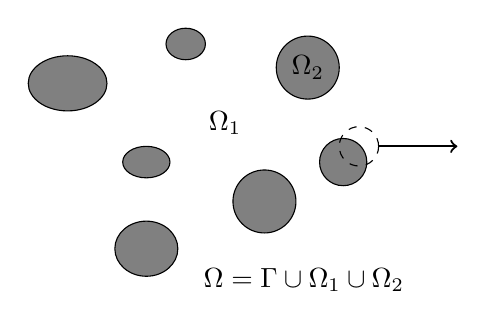
\begin{tikzpicture}
        \foreach \x/\y/\ra/\r in {
        1/3/0.2/0.25,
        2.55/2.7/0.4/0.4,
        0.5/0.4/0.35/0.4,
        2/1/0.4/0.4,
        3/1.5/0.3/0.3,
        0.5/1.5/0.2/0.3,
        -0.5/2.5/0.35/0.5}{
            \draw[fill=gray](\x,\y) ellipse(\r cm and \ra cm);
        }
        \draw[dashed](3.2,1.7)circle(0.25);
        % \draw[thick,->](3.2,1.7)++(0.1767,0.1767)--++(0.4,0.4)--++(1,0);
        \draw[thick,->](3.2,1.7)++(0.25,0)--++(1,0);
        \draw(2.55,2.7)node{$\Omega_2$};
        \draw(1.5,2)node{$\Omega_1$};
        \draw(2.5,0)node{$\Omega = \Gamma \cup \Omega_1 \cup \Omega_2$};
        % \draw(2.5,-1)node{$\Gamma = \sum_\alpha \Gamma_\alpha$};
        % \draw(2.5,-0.5)node{$\Omega_2 = \sum_\alpha \Omega_\alpha$};
    \end{tikzpicture}
    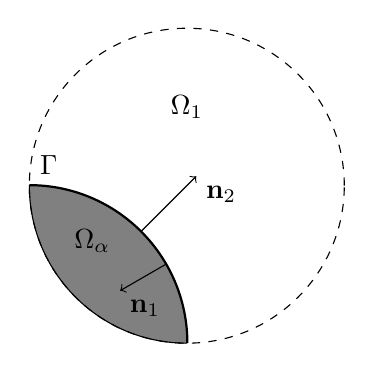
\begin{tikzpicture}%[scale = 0.9]
        \draw[very thick](0:2)arc(0:90:2)node[above right]{$\Gamma$};
        \draw[fill=gray](0:2)arc(0:90:2)arc(180:270:2);
        \draw[dashed](2,2)circle(2);
        \draw[->](1.42,1.42)--++(0.7,0.7)node[below right]{$\textbf{n}_2$};
        \draw[->](1.73,1)--++(-0.577,-0.333)node[below right]{$\textbf{n}_1$};
        \draw(2,3)node{$\Omega_1$};
        \draw(0.8,1.3)node{$\Omega_\alpha$};
    \end{tikzpicture}
    \caption{Domain definitions and scheme of the topology of dispersed two-phase flows.}
    \label{fig:Scheme}
\end{figure}
We consider a system consisting of two phases, separated by a sharp interface $\Gamma(t)$ which evolves over time. 
Each phase subdomain is denoted $\Omega_1(t)$ and $\Omega_2(t)$ for the continuous phase ($1$) and the dispersed phase ($2$) respectively (see \ref{fig:Scheme}). 
The mathematical and physical definition of $\Gamma(t)$ is by no means straightforward, therefore, the interested reader is refereed to \cite{bothe2022sharp} to have a deeper understanding of sharp interface modeling. 
The entire domain, denoted as $\Omega$, is defined as the union of $\Omega_1$, $\Omega_2$, and $\Gamma$.
To track the position of the phase indexed $k$ and the interfaces, we introduce the phase indicator function and the interface indicator function, 
\begin{align}
    \chi_k(\textbf{x},t) =  \left\{
      \begin{tabular}{cc}
        $1 \;\text{if} \;\textbf{x} \in \Omega_k(t)$\\
        $0 \;\text{if} \;\textbf{x} \notin \Omega_k(t)$
      \end{tabular}
      \right.
      \text{for $k = 1,2$},
    %   \label{eq:PIF}
    && \delta_I(\textbf{x},t) =  \left\{
      \begin{tabular}{cc}
        $1 \;\text{if} \;\textbf{x} \in \Gamma(t)$\\
        $0 \;\text{if} \;\textbf{x} \notin \Gamma(t)$
      \end{tabular}
      \right.,
    %   \label{eq:PIF}
\end{align}
respectively. 
For clarity, we omit the time and position arguments of $\chi_k(\textbf{x},t)$ and $\delta_I(\textbf{x},t)$ in the following sections. 

For the purpose of clarity, we only consider the specific case of the mass, momentum and energy conservation equations for a buoyant dispersed two phase flow.
Equally, we consider a constant density and viscosity in each domain as well as a constant surface tension on the interfaces.

% \subsubsection{Inside the volumes}
Within phase $k$, we note $\rho_k$ the density, $\textbf{u}_k^0$ the local velocity and $E_k^0$ the local total energy per units of mass.
All over the domain $\Omega_k(t)$ the mass, momentum and total energy obey these conservation laws :
\begin{align}
    \label{eq:dt_rho}
    \pddt \rho_k  
    + \div (
        \rho_k\textbf{u}_k^0
    )
    &= 
    0\\
    \label{eq:dt_rhou_k}
    \pddt (\rho_k\textbf{u}_k^0)  
    + \div (
        \rho_k\textbf{u}_k^0\textbf{u}_k^0
        - \bm{\sigma}_k^0 
    )
    &= 
    \rho_k \textbf{g}\\
    \label{eq:dt_rhoE_k}
    \pddt (\rho_kE_k^0)  
    + \div (
        \rho_kE_k^0\textbf{u}_k^0
        + \textbf{q}_k^0
        - \textbf{u}_k^0 \cdot \bm{\sigma}_k^0 
        )
    &= 
    \textbf{u}_k^0 \cdot \textbf{g}  \rho_k
\end{align} 
All along this work the continuous phase will be considered as Newtonian fluid thus, $\bm{\sigma}_1^0 = - p_1^0 \textbf{I} + \bm{\tau}_1^0$ where $\bm{\tau}_1^0$ is the Newtonian stress tensor with $p_1 ^0$ the local pressure and $\bm{\tau}_1^0 = \mu_1[\grad \textbf{u}_1^0+(\grad \textbf{u}_1^0)^T]$ the shear rate. 
The vector $\textbf{q}_k^0$ represent the thermal energy flux and is often model with a Fourier law : $\textbf{q}_k^0 = -\lambda \grad T_k^0$ where $T_k$ is the temperature and $\textbf{g}$ is the acceleration of gravity which will be the only body force in the present problem. 
All along this work the superscript $^0$ indicate that the variable is defied at the local or microscopic scale, in opposition to the averaged or macroscopic quantities that will be presented latter. 

% \subsubsection{On interfaces}

On the interfaces the mass, momentum and total energy balance equations reduce to the common expressions :
\begin{align}
    \label{eq:dt_rho_I}
    \textbf{u}_I = \textbf{u}_k
    &=0, \\
    \Jump{\bm{\sigma}_k^0} 
    &=
    \divI\bm\sigma^0_{I||}
    =
    \gamma\kappa\textbf{n},
    % + \gradI\sigma 
    \label{eq:surface_tension}\\
    \label{eq:dt_rhoI_uI2}
    \Jump{\textbf{u}_k^0 \cdot \bm{\sigma}_k^0}
    &=
     \gamma\kappa\textbf{n}\cdot \textbf{u}_{I}^0\\
    \label{eq:dt_rhoIe_I}
    \Jump{ \textbf{q}_k^0}
    &= 
     0
\end{align}
for the interface kinetic energy and the internal interface energy, respectively. 
Notice that this decomposition is possible only under the assumption of no mass transfer in which case $\textbf{u}_I^0=\textbf{u}_k^0$ for $k =1,2$ and a constant surface tension coefficient.



\section{Lagrangian equations for the dispersed phase}
\label{sec:Lagrangian}

While \ref{eq:dt_chi_k_f_k} and \ref{eq:dt_delta_I_f_I} describe multiphase-flow in a general manner, they do not leverage the topology of the dispersed phase. 
Therefore, in this section, we present a Lagrangian-based model capable of describing the dispersed phase with an arbitrary order of accuracy.

\subsection{Fundamental properties}

At this stage, it is crucial to define some fundamental properties associated to each particle.
Following the strategy of \citet{lhuillier2009rheology,lhuillier1992volume,zaepffel2011modelisation} and \citet[Chapter 2]{morel2015mathematical}
we define the mass, position of center of mass, momentum and total energy of the particle $\alpha$, such as,
\begin{align}
    &m_\alpha(t)
    = \int_{\Omega_\alpha(t)} \rho_2  d\Omega,
    % &&
    &\textbf{x}_\alpha(t)
    = \frac{1}{m_\alpha(t) }\int_{\Omega_\alpha(t)} \rho_2 \textbf{x} d\Omega,\\
    % &&
    &\textbf{p}_\alpha(t) 
    = \int_{\Omega_\alpha(t)} \rho_2 \textbf{u}_2^0 d\Omega,
    % &&
    & m_\alpha E_\alpha(t) 
    = \int_{\Omega_\alpha(t)} \rho_2 [e_2^0 + (u_2^0)^2/2] d\Omega,
    \label{eq:position_and_momentum_def}
\end{align}
respectively. 
Where $\Omega_\alpha$ is the domain occupied by the particle $\alpha$ (see \ref{fig:Scheme}). 
Subsequently, we define the velocity of the particle's center of mass, denoted as $\textbf{u}_\alpha$ which is given by $\textbf{u}_\alpha = \ddt{ \textbf{x}_\alpha}$. 
The derivation of $\ddt {\textbf{x}_\alpha}$ is straightforward but requires some algebra which are detailed in \ref{ap:velocity_definition}. 
The final expression reads,
\begin{equation}
    \textbf{u}_\alpha(t) = \frac{1}{m_\alpha(t)} \left(
        \textbf{p}_\alpha(t)
        +  \int_{\Sigma_\alpha(t)} \rho_2 \textbf{r} (\textbf{u}_I^0 - \textbf{u}_2^0)\cdot \textbf{n}_2 d\Sigma
        \right),
        \label{eq:dt_y_alpha}
\end{equation}
where $\textbf{r}(\textbf{x},t) = \textbf{x} - \textbf{x}_\alpha(t)$. 
In Equation \ref{eq:dt_y_alpha}, it can be observed that the first component of the velocity represents the linear momentum divided by the mass of the particle. 
This corresponds to the mass-averaged velocity over the volume of the particle.
The second term in Equation \ref{eq:dt_y_alpha} arises from the contribution of anisotropic mass transfer across the surface of the particle. 
This mass transfer leads to the motion of the particle's center of mass, thereby contributing to the total velocity.
To illustrate this concept, let us consider a fixed drop with no momentum lying over a very hot plate.
In this scenario, we assume that the plate is sufficiently hot to induce evaporation, specifically on the bottom portion of the drop.
Hence, under the effect of an anisotropic evaporation flux one may expect the second term to be non-negligible.
Consequently, the center of mass of the drop has a non-zero velocity in the opposite direction of the plate, even though the momentum is assumed to be zero.
We can also consider the case of the nucleation of a bubble in water. 
In this case, although the particle momentum is null at all time the center of mass of the particle moves due to the growth of the particle. 
In both cases, we need to take into account the mass transfer term in \ref{eq:dt_y_alpha}, while the first term is negligible. 
Note that \ref{eq:dt_y_alpha} generalized usual expression of the center of mass velocity whom neglect the second term.
In the following, we discard the time dependency notation for all Lagrangian quantities denoted by the subscript $_\alpha$ and also $\Sigma(t)$ and $\Omega_\alpha$.
Nevertheless, the reader must understand that all Lagrangian quantities and integration domains subscribed by $_\alpha$ are time dependent. 

The particle's internal relative motions or the \textit{inner velocity} is given by $\textbf{w}_2^0(\textbf{x},t) = \textbf{u}_2^0(\textbf{x}) - \textbf{u}_\alpha(t)$.
Thus, from its definition in \ref{eq:position_and_momentum_def}, we can rewrite the momentum as follows,
\begin{equation}
    \label{eq:momentum_definition_1}
    \textbf{p}_\alpha
    = m_\alpha \textbf{u}_\alpha
    + \int_{\Omega_\alpha} \rho_2 \textbf{w}_2^0 d\Omega.
\end{equation}
Alternatively, by manipulating \ref{eq:dt_y_alpha}, we obtain,
\begin{equation}
    \textbf{p}_\alpha
    =  m_\alpha \textbf{u}_\alpha
    - \int_{\Sigma_\alpha} \rho_2\textbf{r}(\textbf{u}_I^0 - \textbf{u}_2^0)\cdot \textbf{n}_2 d\Sigma
    \label{eq:momentum_definition}
\end{equation}
Therefore, the momentum of a particle can be seen as a sum of the mean velocity plus the integral of the fluctuation (\ref{eq:momentum_definition_1}), with the latter being equivalent to minus the first moment of mass transfer term (\ref{eq:momentum_definition}).
Indeed, by identification we obtain : $\int_{\Omega_\alpha} \rho_2 \textbf{w}_2^0 d\Omega =\int_{\Sigma_\alpha}  \rho_2\textbf{r} (\textbf{u}_I^0 - \textbf{u}_2^0)\cdot \textbf{n}_2 d\Sigma$. 
The essential aspect of this relation highlighted here is that the internal velocity fluctuations within a fluid particle do not contribute to the total linear momentum $\textbf{p}_\alpha$, as long as the anisotropic mass transfer is negligible.  
Additionally, the total energy $E_\alpha$ can be decomposed following a similar procedure which leads us to, 
\begin{equation*}
    \label{eq:E_alpha_def}
    m_\alpha E_\alpha(t) 
    = m_\alpha e_\alpha 
    + W_\alpha
    + m_\alpha (u_\alpha)^2/2
    % + \textbf{u}_\alpha \cdot \int_{\Omega_\alpha(t)} \rho_2  \textbf{w}_2^0 d\Omega
\end{equation*}
where we introduced the internal kinetic energy : $W_\alpha = \int_{\Omega_\alpha(t)} \rho_2  (w_2^0)^2/2 d\Omega$. 
In that expression mass transfer have been neglected. 
The total energy of a particle is the sum of its internal energy $e_\alpha$, internal kinetic energy $W_\alpha$ and the kinetic energy  due to its own center of mass displacement $u_\alpha^2/2$. 
To gain in understanding, let's express $W_\alpha$ in the case of a solid particle.
The velocity inside a solid particle can be expressed : $\textbf{u}_2^0(\textbf{x}_\alpha + \textbf{r}) = \textbf{u}_\alpha + \textbf{r}\times \bm{\omega}_\alpha$ where $\bm{\omega}_\alpha$ is the angular velocity.  
In this case, $W_\alpha = \bm{\omega}_\alpha\bm{\omega}_\alpha\cdot \mathcal{I}_\alpha$ where $\mathcal{I}_\alpha$ is the inertia matrices of the particle. 
As a matter of facts for solid particles $W_\alpha$ represents the angular kinetic energy for solid particles.
Thus, for particles with fluid internal motion, $W_\alpha$ is just a more general definition of the particle internal kinetic energy. 

\subsection{Conservation laws}
We assign to a particle indexed, $\alpha$, occupying the domain $\Omega_\alpha$ (see \ref{fig:Scheme}) an arbitrary Lagrangian property $q_\alpha$ defined by $q_\alpha  = \intO{ f_2^0(\textbf{x},t) }$.
Similarly, we define $q_{I\alpha} = \intS{ f_I^0(\textbf{x},t) }$ as being an integrated surface property associated to the particle $\alpha$.


To describe the evolution of any arbitrary Lagrangian quantity $q_\alpha$, we need to establish its time derivative.
Since, $q_\alpha$ is an integral quantity with a time-dependent domain of integration, we apply the general Reynolds transport theorem for volume integral (exposed in \ref{ap:math}) to compute its time derivative \citep{morel2015mathematical}.
This yields the following expression :
\begin{equation}
    \ddt  q_\alpha
    = \intO{\left[ \pddt f_2^0 + \div\left(f_2^0\textbf{u}_2^0\right) \right]}\\
    + \intS{ f_2^0 (\textbf{u}_I^0-\textbf{u}_2^0)\cdot \textbf{n}_2 }.
\end{equation}
By substituting the integrand of the first integral on the right-hand side (RHS) with \ref{eq:dt_f_k} we obtain the conservation laws of the quantity $q_\alpha$, namely,  
\begin{equation}
    \ddt  q_\alpha
    = \intO{ s_2^0 }
    + \intS{ \left[
        f_2^0 (\textbf{u}_I^0-\textbf{u}_2^0) 
        + \mathbf{\Phi}_2^0 
        \right] \cdot \textbf{n}_2 },
    \label{eq:dt_q_alpha}
\end{equation}
The first term on the RHS accounts for the total contribution of the source term $s_2^0$ to the particle $\alpha$.
While, The second term on the RHS is the surface integration of the exchange terms, which includes the phase transfer flux $f_2^0 (\textbf{u}_I^0-\textbf{u}_2^0)$ and the diffusive flux $\mathbf{\Phi}_2^0$. 
For clarity, let us consider the specific case of the momentum balance, i.e. when $q_\alpha = \textbf{p}_\alpha$.
In this situation, the first term reads as $\intO{ \rho_2\textbf{g} }$ and represents the total weight acting on the particle $\alpha$. 
Likewise, the second term represents the total source of momentum due to phase transfer, and it is expressed as, $\intS{ \rho_2 \textbf{u}_2^0 (\textbf{u}_I^0-\textbf{u}_2^0)\cdot\textbf{n}_2 }$. 
Lastly, $\intS{ \bm{\sigma}_2^0\cdot\textbf{n}_2 }$ represents the resultant of the hydrodynamic forces acting on the surface of the particle.
It is important to notice that under this form, the exchange terms are expressed as integrals of dispersed phase fields denoted by the subscript $_2$.
Nevertheless, depending on the nature of the dispersed phase, these fields may not always be defined.
For infinitely rigid particles it is indeed the case since, the stress $\bm{\sigma}_2^0$ isn't defined.  
Hence, our objective is to express these exchange terms, in terms of the continuous phase field quantities instead of the dispersed phase field, i.e. in terms of $\mathbf{\Phi}_1^0$ and $\textbf{u}_1^0$ rather than $\mathbf{\Phi}_2^0$ and $\textbf{u}_2^0$. 

To address this issue, let us derive the conservation equation for the integrated surface property $q_{I\alpha}$.
To differentiate time-varying surface integrals within time, we can use the general Leibniz rule (see \ref{eq:Leibnitz}), to derive the following expression :
\begin{equation}
    \ddt  q_{I\alpha}
    = \intS{ \left[
        \pddt f_I^0
        +   \gradI \cdot (\textbf{u}_I^0f_I^0)
    \right]}.
    \label{eq:surface_derivative}
\end{equation}
Substituting the RHS terms of \ref{eq:surface_derivative} using \ref{eq:dt_f_I}, and making use of the surface divergence theorem on closed surfaces (see \ref{eq:surf_div_theorem}), gives,
\begin{equation}
    \ddt  q_{I\alpha}
    = \intS{ 
        s_I^0
    }
    - \intS{ \Jump{
        f_k^0 (\textbf{u}_I^0 - \textbf{u}_k^0)
        + \mathbf{\Phi}_k^0
    }}.
    \label{eq:dt_q_I_alpha}
\end{equation}
This equation can be interpreted as the surface conservation equation for the integrated surface property $f_I$, or as the flux jump condition integrated on a closed surface. 
Notice that $\bm{\Phi}_{I}^0$ isn't present in this balance equation. 
This is due to the fact that as mentioned earlier, only the tangential components of $\bm{\Phi}_{I}^0$ appear inside the surface balance equation, while we perform an integration over a closed surface which is null due to \ref{eq:surf_div_theorem}. 

As discussed above we wish to get rid of $\mathbf{\Phi}_2^0$ in \ref{eq:dt_q_alpha}. To achieve this, we treat the particle's volume and surface as a unified entity and derive a conservation equation for $q_\alpha^\text{tot} = q_\alpha + q_{I\alpha}$. 
This is done by summing \ref{eq:dt_q_alpha} and \ref{eq:dt_q_I_alpha} which leads to, 
\begin{equation}
    \ddt  q_\alpha^\text{tot}
    = 
    \intO{ s_2^0 }
    + \intS{ s_I^0 }
    + \intS{ \left[
        f_1^0 (\textbf{u}_I^0-\textbf{u}_1^0) 
        + \mathbf{\Phi}_1^0 
        \right] \cdot \textbf{n}_2 }. 
    \label{eq:dt_q_alpha_tot}
\end{equation}
This equation is the general form of the linear conservation law of $\chi_2 f_2^0 + \delta_I f_I^0$ for the system consisting of the particle volume $\Omega_\alpha$, and its surface $\Sigma_\alpha$. It is applicable to any particle immersed into a continuous phase following the local conservation,\ref{eq:dt_f_k} and \ref{eq:dt_f_I}.
We refer to this equation as the zeroth-order conservation equation or the linear conservation law for the particle $\alpha$.

Following the same assumption as in \ref{sec:local_eq}, i.e. we consider no mass transfer and weightless interfaces, the Lagrangian  mass, momentum and energy equations for a single particle can be derived using the generic form \ref{eq:dt_q_alpha_tot} and reads as, 
\begin{align}
    \label{eq:dt_m_alpha}
    \ddt m_\alpha
    &= 
    0\\
    \label{eq:dt_p_alpha}
    \ddt (m_\alpha \textbf{u}_\alpha)
    &= 
    m_\alpha\textbf{g}
    +  \intS{\bm{\sigma}_1^0 \cdot \textbf{n}_2}\\
    \label{eq:dt_E_alpha}
    \ddt (m_\alpha E_\alpha + s_\alpha \gamma)
    &= 
    m_\alpha \textbf{u}_\alpha \cdot \textbf{g}
    +\textbf{u}_\alpha \cdot \intS{\bm{\sigma}_1^0 \cdot \textbf{n}_2}
    +\intS{\textbf{w}_1^0 \cdot \bm{\sigma}_1^0 \cdot  \textbf{n}_2} 
    - \intS{\textbf{q}_1^0 \cdot \textbf{n}_2}
\end{align}
where  $\intS{  \bm{\sigma}_1^0 \cdot \textbf{n}_2 }$ is the resultants of the hydrodynamic force and $\intS{ \textbf{q}_1^0 \cdot \textbf{n}_2 }$ is the resultants of the surface heat flux. 
The second term on the right hands side of the energy equation is the work produced by the mean force and the translational motion of the droplets, while $\intS{\textbf{w}_1^0 \cdot \bm{\sigma}_1^0 \cdot  \textbf{n}_2}$ is the work produced by the local forces and local motion of the fluid at the surface of the particle.
Since we integrated the energy over the particle's volume and its surface, we explicitly made appear the surface energy $\gamma s_\alpha$ within the derivative operator. 
Note that these equations does not explicitly account for inter-particle interactions. 
However, it is possible to include manually such forces by noticing that the surface external stress flux $\bm{\sigma}_1^0$ is the sum of hydrodynamic and particles-particles interaction forces, regardless it is pure contact forces from direct contact or a force mediated through the carrier fluid.
From this consideration it is possible to split every term involving the stress $\bm{\sigma}_1^0$ into two terms representing these contributions. 
Same comments can be made for the heat flux $\textbf{q}_1^0$. 
Although this distinction is important, for purpose of clearly we will stay general, and we will keep the fluxes $\bm{\sigma}_1^0$ and $\textbf{q}_1^0$ as such. 

In the spirit of the energy decomposition exposed in \ref{eq:E_alpha_def} the total energy equation can be split into three equations, one for the center of mass kinetic energy, internal motion and internal kinetic energy, namely,  
\begin{align}
    \label{eq:dt_u2_alpha}
    \frac{1}{2}\ddt (m_\alpha u_\alpha^2)
    &= 
    \textbf{u}_\alpha\cdot
    \textbf{g}m_\alpha
    + 
    \textbf{u}_\alpha\cdot
    \textbf{f}_\alpha,\\
    \label{eq:dt_w2_alpha}
    \ddt (W_\alpha + \gamma s_\alpha)
    &= 
    \intS {\textbf{w}_1^0 \cdot \bm{\sigma}_1^0 \cdot \textbf{n}_2 }
    - \intO{ \bm{\sigma}_2^0 : \grad\textbf{u}_2^0 }
    \\
     \label{eq:dt_e_alpha}
    \ddt (m_\alpha e_\alpha )
    &= 
     \intO{ \bm{\sigma}_2^0 : \grad\textbf{u}_2^0  }
    -  \intS{\textbf{q}_1^0\cdot \textbf{n}_2 } 
\end{align}
respectively. 
Note that in \citet{eq:dt_w2_alpha} the use of \ref{eq:dt_rhoI_uI2} makes appear explicitly the derivative of the surface energy $s_\alpha \gamma$. 
Note that under this form we see that the energy loss in the deformation represented by $W_p$ will be gathered in the surface energy which will in turn act as a source term in the internal kinetic energy motion.
The surface tension plays the role as a spring in the energy balance.   
From this set of equation we can easily see that the rate of dissipation terms $\intS{\bm{\sigma}_2^0 : \grad\textbf{u}_2^0}$ represent an energy sink in the equation of $W_\alpha$ while it is a source term in the internal energy equation. 
As it has been observed in the previous section, this terms convert the energy of internal motion to molecular agitation. 
However, the interplay between the center of mass  kinetic energy and the internal fluctuation is not obvious and has no common term with the heat and internal kinetic energy equation.
In fact, we will see that the transfer between these scales is archived thought the fluid phase pseudo turbulent energy. 


Finally, we would like to highlight that  due to the consideration of closed surface, the diffusive flux $\mathbf{\Phi}_I$, plays no role at all in \ref{eq:dt_q_alpha_tot}.
Therefore, in the case of the linear momentum conservation law, the contribution of the surface tension forces exposed in \ref{eq:surface_tension}, do not contribute to the momentum balance in \ref{eq:dt_p_alpha}.
As a consequence, even in the presence of local Marangoni forces, the resultant of the local surface tension forces would cancels out in the linear momentum balance.
This fact has already been demonstrated by \citet{hesla1993note} who showed that the surface tension force does not contribute to the linear and angular momentum balance. 
Here, we have provided the general proof that the interfacial diffusive flux $\mathbf{\Phi}_I^0$, which is present at the local scale according to \ref{eq:dt_f_I}, does not contribute to the zeroth-order conservation law of a particle with a closed surface.
This is therefore applicable to other conservation equations, such as the surface energy balance or the surface mass balance of constituents, where surface diffusive fluxes are also present \citep{bothe2022sharp,manikantan2020surfactant}. 

Nevertheless, it is known that surface tension forces impact the hydrodynamic of droplets and bubbles \citep{kentheswaran2022direct,pesci2018computational}. 
Therefore, if the diffusive flux of surface are not involved in the linear conservation law, it must appear at some point in the Lagrangian momentum description of  particles. 
To find out where this contribution arise we shall describe the particle with a higher level of accuracy. 
This is the purpose of the next section. 

\subsection{First order moment equations}

To better describe the local properties within the particles, we now introduce the first moment or the dipole of a particle.
We define the first moment of any properties $f_2^0$ and $f_I^0$ by respectively,
\begin{align}
    &\mathcal{Q}_\alpha 
    = \intO{ \textbf{r} f_2^0 },
    &\text{and}&
    &\mathcal{Q}_{I\alpha}
    = \intS{ \textbf{r} f_I^0 },
    \label{eq:first_moment_definition}
\end{align}
where we recall that $\textbf{r} = \textbf{x} - \textbf{x}_\alpha$ is the distance between any point inside $\Omega_\alpha$ or $\Sigma_\alpha$, to the center of mass of the particle $\alpha$.
It is then possible to differentiate these moments with respect to time in order to obtain their conservation laws.
Indeed, considering \ref{eq:dt_f_k}, \ref{eq:dt_f_I} and applying the Leibniz rule for volume and surface integrals (see \ref{eq:Reynolds} and \ref{eq:Leibnitz} respectively), we can show equally that,
\begin{align}
    \ddt {\mathcal{Q}_\alpha}
    &= \intO{ \left(
        \textbf{r} s_2^0         
        + f_2^0  \textbf{w}_2^0 
        - \mathbf{\Phi}_2^0
    \right) },
    + \intS{ \textbf{r} \left[
        \mathbf{\Phi}_2^0
        + f_2^0 (\textbf{u}_I^0-\textbf{u}_2^0)
    \right]\cdot \textbf{n}_2  } 
    \label{eq:dt_Q_alpha}\\
    \ddt {\mathcal{Q}_{I\alpha}}
    &= \intS{ \left(
        \textbf{r}s_I^0
        + f_I^0 \textbf{w}_I^0
        - \mathbf{\Phi}_{I||}^0
    \right) },
    - \intS{\textbf{r} 
    \Jump{\mathbf{\Phi}_k^0
        + f_k^0 (\textbf{u}_I^0 - \textbf{u}_k^0)
    }
    },
    \label{eq:dt_Q_I_alpha}
\end{align}
where $\textbf{w}_I^0 = \textbf{u}_I^0 - \textbf{u}_\alpha$.
The detailed derivation of \ref{eq:dt_Q_alpha} is provided in \ref{ap:moment_derivative}.
The derivation of \ref{eq:dt_Q_I_alpha} follows a similar procedure. 
% \JL{je n'ai pas relu la derivation detaillee en annexe, ... je te fais confiance. par contre en annexe tu ne derive pas le premier moment interfacial. 
% J'imagine que la derivation est la meme encore faut il le preciser. 
% Egalement j'ai regorganise les elements dans les equations precedentes par signification physique. 
% D'ailleurs il y avait des differences dans les deux equations (la premiere $r S$, la seconde $S r$)... 
% Merci de faire attention a ce genre de detail. 
% J'avoue avoir du mal a comprendre l'interpretation physique de l'integrale de la contrainte dans le volume. 
% Comme on en discutait, par exemple pour une particule solide, celle integrale n'est pas determinee, donc il faudrait la remplacer par quelque chose que l'on connait non ? 
% \tb{Dans le cas ou les contrainte ne sont pas defini les degrées de liberté des particules solid font que cette contrainte ne peux ne pas etre prise en compte la partie symmetrique de cette formule 
% permet justement de remonter a la contrainte dans le cas ou elle ne serait pas defini. dans le cas des particue fluid cela a du sens parcontre c'est les contraintes interne qui s'oppose a la deformations}}
% \JL{
%  Enfin bon a discuter (pas forcement ici). 
%  je pense que c'est un point important. 
% }\tb{cela va etre discuter dans la partie ou on traitre du momentum non ?}
% \JL{
%  Par ailleurs dans quel cas l'integrale des fluctuations $w_2$ est elle nulle ? 
%  pour une particule solide est ce le cas ? 
%  j'imagine que oui ? 
%  J'imagine que tout cela est traite plus tard (dans la derniere section), mais ca me parait crucial de bien expliquer a quoi servent ces termes et dans quel cas ils sont nuls. 
%  \tb{dur a expliquer pour une quantité general }
%  }\JL{
%  Une maniere d'expliciter tout cela pourrait etre de separer j'imagine le premier moment (au moins pour la vitesse) en une partie symmetrique et une partie anti symmetrique pour bien differencier ce qui est lie a la vitesse angulaire et la deformation. 
%  \tb{dans ce cas il faudrait donner l'application du momentum maintenant ce qui change le plan}}
In \ref{eq:dt_Q_alpha}, we recognize the first moment of the source term $s_2^0$, the first moment of the diffusive flux term $\mathbf{\Phi}_2^0\cdot\textbf{n}_2$ and the first moment of phase exchange term, $f_2^0 (\textbf{u}_I^0-\textbf{u}_2^0)\cdot\textbf{n}_2$. 
Additionally, two supplementary terms appear in \ref{eq:dt_Q_alpha}, namely : the integral of the diffusive flux $\mathbf{\Phi}_2^0$, and a term related to the fluctuation of the internal velocity $f_2^0 \textbf{w}_2^0$.
Similar observations can be made for the fist moment of surface equation \ref{eq:dt_Q_I_alpha}, as it shares similarities with \ref{eq:dt_Q_alpha}. 
In particular, it is worth noting the presence of the surface diffusive flux $\mathbf{\Phi}_{I||}^0$ in \ref{eq:dt_Q_I_alpha}.
This term will be further discussed and analyzed in the following. 

For similar reason than the linear conservation equations, we sum \ref{eq:dt_Q_alpha} and \ref{eq:dt_Q_I_alpha} to expresses the conservation equation of the total first moment $\mathcal{Q}_\alpha^\text{tot} = \mathcal{Q}_\alpha + \mathcal{Q}_{I\alpha}$.
This leads to the following expression:
\begin{multline}
    \ddt {\mathcal{Q}_\alpha^\text{tot}}
    = \intO{ \left(
        \textbf{r} s_2^0         
        + f_2^0  \textbf{w}_2^0 
        - \mathbf{\Phi}_2^0
    \right) }
    + \intS{ \left(
        \textbf{r}s_I^0
        + f_I^0 \textbf{w}_I^0
        - \mathbf{\Phi}_{I||}^0
    \right) }
    + \intS{ \textbf{r} \left[
        \mathbf{\Phi}_1^0
        + f_1^0 (\textbf{u}_I^0-\textbf{u}_1^0)
    \right]\cdot \textbf{n}_2  }. 
    \label{eq:dt_Q_alpha_tot}
\end{multline}
Likewise, conservation laws can be derived for an arbitrary $n^{th}$ order moments of volume and surface, i.e. for
\begin{align}
    \mathcal{Q}_\alpha^n
    = \intO{
        \textbf{r}^n
        f_2^0 },
        && \text{and} &&
    \mathcal{Q}_{I\alpha}^n
    = \intS{
        \textbf{r}^n
    f_I^0 },
    \label{eq:Q_n_definition}
\end{align} 
respectively, where $\textbf{r}^n$ is the shorthand for the tensor product $\textbf{r}^n = \underbrace{\textbf{rr}\ldots \textbf{rr}}_{n\text{ times}} $ with $n$ times itself. 
It can be shown that the derivative with time of do not involve any additional terms than in \ref{eq:dt_Q_alpha} and \ref{eq:dt_Q_I_alpha}, but rather just the $n^{th}$ order moments of the already presented terms.
We provide the full derivation of $\ddt{ \mathcal{Q}_\alpha^n}$ in \ref{ap:Moments_equations}.
In short, these higher order moments describe the distributions of the local quantities $f_2^0$ and $f_I^0$ inside the domain $\Omega_\alpha$ and $\Sigma$ respectively.
Consequently, an infinite number of moments would be theoretically necessary to recover the fields of $f_2^0$ and $f_I^0$  within $\Omega_\alpha$ and $\Sigma$. 


% At this stage it is difficult to interpret the physical meaning behind these moments equations. 
% Therefore, to gain in understanding. 
We now discuss the second order moment of mass and first order moment of momentum conservation equations. 
In the following examples, we consider the same hypothesis as in thep previous section. 
Following \ref{eq:Q_n_definition} we define the second-order moment of mass and the first-order moment of momentum as respectively,
\begin{equation}
    \mathcal{M}_\alpha 
    = \intO{ \rho_2 \textbf{r} \textbf{r} }
    \;\;\;\text{and}\;\;\;
    \mathcal{P}_\alpha 
    = \intO{ \rho_2 \textbf{r} \textbf{u}_2^0 }.
    \label{eq:first_moment_of_momentum_def}
\end{equation}
Note that $\mathcal{M}_\alpha$ is analogous to the inertia tensor $\mathcal{I}_\alpha$ in solid mechanics, and they are related through the expression, $\mathcal{I}_\alpha = \text{tr}(\mathcal{M}_\alpha)\textbf{I} - \mathcal{M}_\alpha$.
At constant density the tensor $\mathcal{M}_\alpha$ describes the second moment of the volume distribution around the particle's center of mass.
In order to provide a clearer physical interpretation to the moment of momentum tensor, we decompose $\mathcal{P}_\alpha$ into two distinct part, namely,
$\mathcal{P}_\alpha = \mathcal{S}_\alpha+\mathcal{T}_\alpha$ where $\mathcal{S}_\alpha$ represents the symmetric part and $\mathcal{T}_\alpha$ is the antisymmetric part of $\mathcal{P}_\alpha$.
The tensors $\mathcal{S}_\alpha$ and $\mathcal{T}_\alpha$ correspond respectively to the stretching and angular momentum of the particle $\alpha$. 
The tensor $\mathcal{S}_\alpha$ quantifies how fast and in which direction the particle get elongated or flattened, in other worlds it represents the rate of deformation experienced by the particle.
The tensor $\mathcal{T}_\alpha$ is related to the angular momentum of the particle. 
In this study we use the pseudo vector $\bm{\mu}_\alpha = \intO{ \rho_2 \textbf{r} \times \textbf{u}_2^0 }$ to express this quantity. 
Indeed, both  $\mathcal{T}_\alpha$ and $\bm{\mu}_\alpha$ represent the angular momentum and are related through $(\bm{\mu}_\alpha)_i = \epsilon_{ijk} (\mathcal{P}_\alpha)_{jk}= \epsilon_{ijk} (\mathcal{T}_\alpha)_{jk}$, where $\epsilon$ is the third order alternating unit tensor. 
Lastly, we also introduce the scalar $\mathcal{D}_\alpha = \text{tr}(\mathcal{P}_\alpha) = \frac{1}{3}\int0{ \rho_2 \textbf{r} \cdot \textbf{u}_2^0 }.$, which quantifies the rate at which the particle is being compressed.

Injecting, $f_2 = \rho_2$ in the second-order moment equation derived in \ref{ap:Moments_equations} we obtain :
\begin{equation}
    \ddt {\mathcal{M}_\alpha}=2\mathcal{S}_\alpha. 
    \label{eq:dt_M_alpha}
\end{equation}
which is the general form of the second moment of mass conservation equation. 
From \ref{eq:dt_M_alpha} we deduce that the evolution of the distribution of mass of a particle is solely motivated by the stretching of momentum, denoted by $\mathcal{S}_\alpha$. 
This implies that the angular momentum (not to be confused with the angular velocity) plays no-role in the evolution of the second moment of the mass distribution. 
Note that if the particle has a constant $\mathcal{M}_\alpha$ under change of reference frame, such as for spherical particles where we can write $\mathcal{M}_\alpha= \frac{a^2 m_\alpha}{5} \textbf{I}$, then the stretching of momentum is null $\mathcal{S}_\alpha=0$.
This argument has no restriction on the internal particle motion. 
Additionally, applying the trace operator on both sides of \ref{eq:dt_M_alpha}, yields the interesting relation : $\ddt {\text{tr}(\mathcal{M}_\alpha)}=2\mathcal{D}_\alpha$.
Therefore, we can state that $\text{tr}(\mathcal{M}_\alpha) = \lambda^\alpha_1(t)+\lambda^\alpha_2(t)+\lambda^\alpha_3(t)$, with $\lambda_i^\alpha$ for $i=1,2,3$, being the eigenvalues of $\mathcal{M}_\alpha$.
For unreformable particles it is evident that the eigenvalues are not function of time, therefore $\ddt{ \text{tr}(\mathcal{M}_\alpha)}=0$.  
Consequently, $\mathcal{D}_\alpha$ has the notable property of being null whenever the particle shape remain constant, irrespective of the orientation.
The third invariant of this tensor can be shown to be related to the volume of the particle. 

Now, that we described the shape of the particle through its with the symmetric part of the moment of momentum we might need an equation for the moment of momentum. 
This equation is derived injecting $\mathcal{Q}_\alpha = \mathcal{P}_\alpha$ in \ref{eq:dt_Q_alpha_tot}, it reads, 
\begin{equation}
    \ddt {\mathcal{P}_\alpha}
    = \intO{ \left(
        \rho_2  \textbf{w}_2^0 \textbf{w}_2^0 
        - \bm{\sigma}_2^0
    \right) }
    - \intS{ 
        \gamma \textbf{I}_{||}
    }
    + \intS{ \textbf{r}\bm{\sigma}_1^0\cdot \textbf{n}_2} 
    \label{eq:dt_P_alpha}
\end{equation}
The last term on the right hands side of \ref{eq:dt_P_alpha} represents the first hydrodynamic moment of the force traction on the particle surface.
It is commonly  decomposed into a symmetric and an antisymmetric part defined as, 
\begin{align}
    \label{eq:M_decomposition}
    \mathscr{S}_{\alpha,ij}^*
    &= \frac{1}{2}  \intS{ \left[
        r_i(\sigma_{1,jk}^0 n_k)
        + (\sigma_{1,ik}^0 n_k)r_j
        \right]}
    %     - \frac{\delta_{ij}}{3}\int_{\Sigma_\alpha} \left[
    %         r_l(T_{lk}n_k)
    % \right]d\Sigma
    \\
    \mathscr{L}_{\alpha,ij}
    &= \frac{1}{2}  \intS{ \left[
        r_i(\sigma_{1,jk}^0 n_k)
        - (\sigma_{1,ik}^0 n_k)r_j
    \right]}, \nonumber
\end{align}
respectively. 
It will be shown in \ref{sec:averaged_eq} that $\mathscr{S}_\alpha$ is related to a quantity called the stresslet. 
We introduce the torque vector as $\textbf{t}_\alpha = \intS{ \textbf{r} \times (\bm{\sigma}_1\cdot \textbf{n}_2) }$ which is related to the skew symmetric part of the first moments $t_{\alpha,i} = \epsilon_{ikj} \mathscr{L}_{\alpha,jk}$. 
Each of the other terms appearing in \ref{eq:dt_P_alpha} is discussed in further detail in the following.
 

The conservation equation of the angular momentum $\bm{\mu}_\alpha$ is obtained by taking the double contracted product of \ref{eq:dt_P_alpha} with $\epsilon$, which gives the simple expression :
\begin{equation}
    \ddt\bm{\mu}_\alpha
    =  
    % \textbf{t}_\alpha.
    \intS{ \textbf{r} \times \bm{\sigma}_1^0\cdot \textbf{n}_2 }
    \label{eq:dt_mu_alpha}
\end{equation}
Notice that every terms on the RHS of \ref{eq:dt_P_alpha} vanish due to their symmetric nature apart from the first hydrodynamic moment $\mathcal{M}_\alpha$.
Particularly, the surface tension terms do not appear in the angular momentum balance, which is consistent with the findings of \citet{hesla1993note}. 
As a consequence, the surface tension has no effect on the angular momentum regardless of the particle's shape. 
In the literature it is common to include the torque due to inter-particular interactions in the angular momentum balance, as it is done in \citet{jackson1997locally} and \citet{zhang1997momentum}.
Therefore, we remind the reader that $\bm{\sigma}_0^1$ contain interaction forces thus $\textbf{t}_\alpha$ includes particles-particles interactions.


Taking the symmetric part of \ref{eq:dt_P_alpha}, yield an equation for the stretching of momentum, which can be written as,
\begin{equation}    
    \ddt{\mathcal{S}_\alpha}
    =  \intO{
        \rho_2\textbf{w}_2^0 \textbf{w}_2^0
        - \bm{\sigma}_2^0}
        - \sigma\intS{\textbf{I}-\textbf{nn}}
        + \frac{1}{2}\intS{(\textbf{r}\bm\sigma_2^0+ \bm\sigma_2^0\textbf{r})\cdot \textbf{n}}
    \label{eq:dt_S_alpha}
\end{equation}
\tb{introduce the second order derivative here ? }
One might immediately recognize that this equation is in facts an extension to Batchelor’s famous result, 
\begin{equation*}
    \intO{\bm{\sigma}_2^0}
    + \intO{\bm{\sigma}_I^0}
    = \frac{1}{2}\intS{(\textbf{r}\bm\sigma_2^0+ \bm\sigma_2^0\textbf{r})\cdot \textbf{n}}
\end{equation*}
% \tb{it is also an extension to dolata recent results for teh first and second moment equation }
which has been used widely in stokes flow theory to express the unknown internal stress within solid particles in terms of surface integral, i.e. the stress let $\intS{(\textbf{r}\bm\sigma_2^0+ \bm\sigma_2^0\textbf{r})\cdot \textbf{n}}$.
This relation is the main tools used to express the bulk stress of a suspension, it eventually leads to the computation of the famous Einstein equivalent viscosity upon having an analytical formula for $\intS{(\textbf{r}\bm\sigma_2^0+ \bm\sigma_2^0\textbf{r})\cdot \textbf{n}}$. 
Therefore, the significant aspect of \ref{eq:dt_S_alpha} is that it can be interpreted as a generalized equation for the integrated stress tensor within the volume of the particle.
This will become particularly relevant when determining the total stress of an inertial suspension as it will be mentioned in \ref{sec:averaged_eq}.
On the right hands side of \ref{eq:dt_S_alpha} we can identify several terms: 
the internal kinetic energy $\intO{\rho_2\textbf{w}_2^0\textbf{w}_2^0 }$; 
the integral of the particle internal stress $\intO{ \bm{\sigma}_2^0
 }$; 
the integral of the surface stress $\intS{ \sigma (\textbf{I}- \textbf{nn}) }$; 
and the stresslet tensor, $\intS{(\textbf{r}\bm\sigma_2^0+ \bm\sigma_2^0\textbf{r})\cdot \textbf{n}}$ introduced earlier.
Based on \ref{eq:dt_M_alpha} we can infer that the evolution of $\mathcal{M}_\alpha$ is driven by the internal kinetic energy and the stresslet.
However, it is being counteracted by surface tension forces and internal stresses which tend to oppose the deformation of the particle. 
Therefore, if the surface tension forces play no role in the linear and angular momentum equation, it does impact the stretching of momentum $\mathcal{S}_\alpha$.
As a consequence, the surface tension force impact the hydrodynamic behavior of a particle solely through its action on $\mathcal{S}_\alpha$, which is related to the shape of a particle through \ref{eq:dt_M_alpha}.
As remarked by \citet{batchelor1970stress}, since the surface tension force oppose the deformation of a particle, it can be understood as an elastic force. 
Which, as it will be shown in \ref{sec:averaged_eq} has a role on the bulk stress of the suspension. 
Additionally, note that \ref{eq:dt_S_alpha} can be seen as a formula to reformulate the integral of the internal stress $\pOavg{\bm{\sigma}}$.
Equally, in \ref{ap:moment_derivative} we show how to derive the higher order moment of momentum equations, which can also be viewed as formulas for the higher moments of the internal particle stress. 
It is interesting to mention that in a recent study of \citet{dolata2021faxen} they use energy method and recover the first two moments of momentum equations hidden into another but equivalent form, valid in the stokes flow regime. 


% Lastly, by taking the trace of \ref{eq:dt_Q_alpha_tot}, directly yields the scalar equation :
% \begin{equation}
%     \ddt {\mathcal{D}_\alpha}
%     = \intO{ \left(
%         \rho_2 \textbf{w}_2^0 \cdot \textbf{w}_2^0
%         - \bm{\sigma}_2^0 : \textbf{I}
%         \right) }
%         - 2 s_\alpha \gamma
%         + \text{tr}(\textbf{M}_\alpha)
%     \label{eq:dt_D_alpha}
% \end{equation}
% which correspond to the isotropic work balance within the particle's volume and surface. 
% As a matter of fact, the rate of compression of a particle, denoted by the scalar $\mathcal{D}_\alpha$ evolves according to : 
% the internal kinetic energy, $\intO{\rho_2 \textbf{w}_2^0 \cdot \textbf{w}_2^0 }$;
% the trace of the integral of the hydrodynamic stresses, $\intO{ \text{tr}(\bm{\sigma}_2^0)}$; 
% the surface energy $\intS{ \gamma }$; 
% and the trace of the hydrodynamic first moment, $\text{tr}(\textbf{M}_\alpha)$.
% To provide a concrete insight of the physical implication of the above equation, 
% % we consider the example of spherical bubbles with time dependent radius $a_\alpha(t)$ and show that from the scalar moment of momentum equation one can recover the Rayleigh-Lamb-Plesset equation. 
% % Indeed, in this situation, the internal velocity can be expressed as, $\textbf{w}_2^0 = \frac{d a_\alpha(t)}{dt} \frac{\textbf{r}}{a_\alpha(t)}$, which makes the scalar moment of momentum equation as, 
% % \begin{equation*}
% %     \frac{3}{5}\rho_2 a_\alpha(t)\frac{d^2 a_\alpha(t)}{dt^2}
% %     = \intO{(\bm{\sigma}_2^0)_{kk}}
% %     - a_\alpha(t)\intS{\textbf{n}\cdot \bm{\sigma}_2^0 \cdot \textbf{n}}
% %     - 2 \gamma s_\alpha
% % \end{equation*}
% % Upon making use of the constitutive law $\bm{\sigma}_k^0 = -p_k \textbf{I} + \mu_k (\grad \textbf{u}_k^0 + (\grad \textbf{u}_k^0)^T) + \zeta_k \div \textbf{u}$ which we will consider true in both phases except that for the carrier fluid $\zeta_1=0$, one obtain, 
% \begin{equation*}
%     (\rho_1 + \frac{1}{5}\rho_2)a_\alpha\frac{d^2 a_\alpha}{dt^2}
%     + \frac{3}{2}\rho_1\left(\frac{d a_\alpha}{dt}\right)^2
%     + (4\mu_1 + 3\zeta_2) \frac{1}{a_\alpha}\frac{d a_\alpha}{dt}
%     = \smallavg{p_1}{\Sigma_\alpha} - \smallavg{\sigma}{\Sigma_\alpha} - \frac{2\gamma}{a_\alpha}
% \end{equation*}
% where,  $\smallavg{p_1}{\Sigma_\alpha}$ and  $\smallavg{\sigma}{\Sigma_\alpha}$ are the surface-averaged external pressure and surface tension coefficient respectively, and $\smallavg{p_2}{\Omega_\alpha}$ represent the volume-averaged internal pressures.
% We indeed recovered the Rayleigh-Lamb-Plesset equation. 
% \tb{Re do the derivation}
%  we examine a single spherical fluid particle of radius $a$, immersed in a steady flow such that $\textbf{u}^0 = 0$ on $\Omega$. 
% In this situation, the stress tensor can be written as $\bm{\sigma}_k = \textbf{I} p_k^0$ for $k = 1, 2$ where $p_k^0$ is the local pressure in the phase $k$. 
% Therefore, applying these considerations to \ref{eq:dt_D_alpha} yields the relation, 
% \begin{equation*}
%     \smallavg{p_2^0}{\Omega_\alpha} 
%     - \smallavg{p_1^0}{\Sigma_\alpha}
%     =
%     \frac{2}{a} s_\alpha \gamma
%     \label{eq:Laplace_law}
% \end{equation*}
% Under this form it is evident that \ref{eq:Laplace_law} represent the well-known Laplace's Law. 
% Additionally, in light of \ref{eq:dt_M_alpha}, the scalar moment of momentum equation can be interpreted as an equilibrium equation for the particle internal mass distribution, or moment of inertia, since $\ddt{\text{tr}(\mathcal{M}_\alpha)} = 2 \mathcal{D}_\alpha$. 
% From this argument and \ref{eq:dt_D_alpha}, one is able to derive the \textit{Rayleigh-Plesset} equation by considering compressible spherical particles with a non-constant particles radius $a_\alpha(t)$ and assuming an internal velocity written as, $\textbf{w}^0_2 = \frac{d a_\alpha(t)}{dt}  \frac{\textbf{r}}{a_\alpha(t)}$. 
% % A demonstration of this derivation can be found in the class of \tb{CITER LE COURS DE Lhuillier}. 
% By the mean of kinetic theory \citet{zhang1994averaged} derived the \textit{Rayleigh-Plesset} equation under an equivalent but averaged form.
% What we demonstrated is that the scalar moment of momentum balance, i.e. \ref{eq:dt_D_alpha} quantify any isotropic dynamical related to a particle. 


% 
\subsection{Spheroidal fluid particles}

Many studies have been conducted to determine the influence of the droplets' deformation on suspension Rheology \citet{goddard1967nonlinear,lhuillier1987phenomenology,maffettone1998equation}.
Most of the authors considered the Rheology of such an emulsion for neutrally buoyant droplets in shearing flow. 
In this work we would to present a first glimps  of the form Rheology of deformable droplets or bubbles with relative motion. 
As a first step to describe the rheology we are interested in the kinematic and dynamic of a single deformable drop. 
In \ref{sec:Exemples} we study the case of 

\subsubsection*{The drop shape}

In this study we consider spheroidal particles described by a conformation tensor that we note $\textbf{C}_\alpha(t)$.  
This tensor is defined such that its eigenvalues are the dimensionless square length of the semi-axis of the spheroid minus one, such that $\textbf{C}_\alpha = (a_1^2/a^2 - 1) \textbf{pp} + (a_2^2 /a^2 - 1) (\textbf{I}-\textbf{pp})$ where $r$ is the radius of the sphere of same volume and \textbf{p} the orientation vector of the particle (see Figure \ref{fig:scheme2}).  
In this way $\textbf{C}_\alpha = 0$ when the particle is spherical and  $\textbf{C}_\alpha + \textbf{I}$ is equivalent to the Cauchy strain tensor well-defined in solid mechanics \citet{mwasame2017macroscopic}. 
In a general coordinate system the point on the surface of the spheroid verify the relation, 
\begin{equation*}
    \textbf{r}\cdot(\textbf{C}_\alpha + \textbf{I})^{-1}\cdot\textbf{r} = a^2,
\end{equation*}
\tb{is it really usefull to define this traceless matrix instead of the actual ellipse}
where $^{-1}$ is the inverse operator.  
One can verify that the second order moment of mass of the particles is related to the conformation tensor through, $\textbf{M}_\alpha = \frac{m_\alpha  a^2}{5} (\textbf{C}_\alpha + \textbf{I})$. 
The last property of the of this tensor is that it the constant volume conservation can be obtained by ensuring that $\text{det}(\textbf{C}_\alpha +\textbf{I}) = (a_1a_2^2)^2 /(a^6) = 1$. 
\begin{figure}[h!]
    \centering
    \hfill
    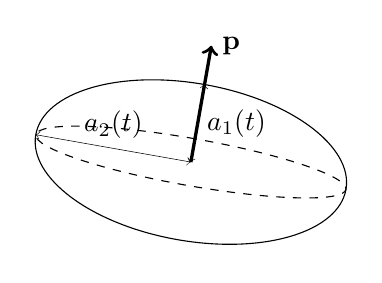
\begin{tikzpicture}[rotate=80]
        \draw(0,0) ellipse (1 cm and 2 cm);
        \draw[dashed](0,0) ellipse (0.3 cm and 2 cm);
        \draw[<->,very thin](0,0) --++ (1,0)node[midway,right]{$a_1(t)$};
        \draw[->,very thick](0,0) --++ (1.5,0)node[right]{$\textbf{p}$};
        \draw[<->,very thin](0,0) --++ (0,2)node[midway,above]{$a_2(t)$};
    \end{tikzpicture}
    \hfill
    \caption{Scheme of an  oblate spheroid oriented along the unit vector \textbf{p} with $a_1(t)$ and $a_2(t)$ the length of the semi axes of the spheroid.}
\end{figure}


\subsubsection*{The droplet internal velocity}

The internal velocity of a solid elastic particle following a homogeneous linear deformation can be described such as $\textbf{w}_2^0 = \bm\Gamma_\alpha \cdot \textbf{r}$ where we have introduced, $\bm\Gamma_\alpha$, the mean velocity gradient inside the particle, which symmetric part : $\textbf{E}_\alpha$, represents the rate of strain, and skew symmetric part : $\bm\Omega_\alpha$, represents the angular velocity. 
Even through the velocity fields $\textbf{w}_2^0 = \bm\Gamma_\alpha \cdot \textbf{r}$  can apply for liquid deforming droplet, an additional flow is present. 
Indeed, from the solution of the stokes equations we can predict the flow within a spherical isolated drop immersed in an unbounded fluid. 
Especially, we know that an solated droplet in translation exhibit internal motion known as Hill vortexes, see \ref{fig:flowlines} (b). 
For a drop immersed in an unbounded linear flow we can also derive an analytical solution such that $\textbf{w}_2^0 \sim \textbf{rrr}$, see \ref{fig:flowlines} (a). 
Therefore, the droplet's internal velocity fields is constituted with a component accounting for the complex internal motions that does not alter the shape of the drop, and another component that account for the linear deformation of the drop.  
\begin{figure*}
    \centering
    \begin{tikzpicture}
        \node (img3) at (0.6\textwidth,0) {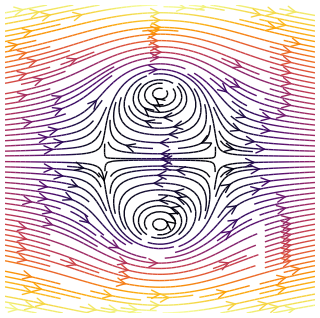
\includegraphics[width=0.3\textwidth,angle=270]{image/Rising_def_Stokes.png}};
        \node (img2) at (0.3\textwidth,0) {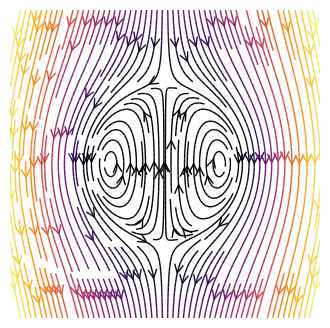
\includegraphics[width=0.3\textwidth]{image/Rising_Stokes.png}};
        % \draw (0.45\textwidth,0)node{$\rightarrow$};
        % \draw (0.45\textwidth,0.4cm)node{$\bm\Gamma_\alpha\cdot \textbf{r}$};
        \node (img1) at (0.0\textwidth,0) {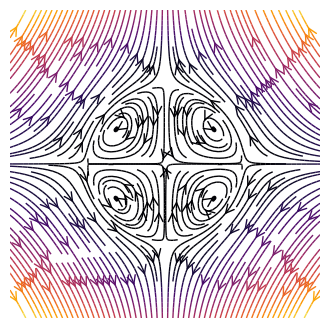
\includegraphics[width=0.3\textwidth]{image/Shear_Stokes.png}};
        \draw (img3.south)node{(c)};
        \draw (img2.south)node{(b)};
        \draw (img1.south)node{(a)};
    \end{tikzpicture}
    \caption{Three examples of steady state flow lines plots of an isolated droplet immersed into a viscous fluid. 
    (a) Rising sphere in uniform stokes flow (analytical solution in \ref{ap:Translating_sphere}). 
    (b) Fixed droplet in extensional flow (analytical solution in \ref{ap:Translating_sphere}).
    (c) Deformed droplet in rising motion (analytical solution of \citet{taylor1964deformation}). }
\end{figure*}
Consequently, the particle internal velocity might be written, 
\begin{equation}
    \textbf{w}_{2,i}^0(\textbf{x}_\alpha)
    = \bm\Gamma_{\alpha,ik}(t) \cdot \textbf{r}_k
    + \textbf{w}^{s}_{2,i}(t,\textbf{r})
    =\bm{\Omega}_{\alpha,ik}\cdot \textbf{r}_k
    + \textbf{E}_{\alpha,ik} \cdot \textbf{r}_k
    + \textbf{w}^{s}_{2,i}(t,\textbf{r})
\end{equation}
Where we introduced the vector $\textbf{w}^{s}_2(t,\textbf{r}) =\textbf{w}^{0}_{2,i}(t,\textbf{r})  - \bm\Gamma_{\alpha,ik}(t) \cdot \textbf{r}_k$ which represents all the internal motions that does not alter the drop's shape. 
Examples of such motions are displayed \ref{fig:flowlines}. 


From now on we consider that the internal velocity $\textbf{w}^{s}_2(t,\textbf{r})$ is not part of the particles unknown, but a function entirely determined by the particle and flow properties such that $\textbf{w}^{s}_2(t,\textbf{r}) =f_\textbf{w}(\textbf{u}_\alpha,\textbf{C}_\alpha,\bm\Gamma_\alpha,\textbf{u}_1,\bm \Gamma_1,\phi_2) $, where $\bm\Gamma_1 = \grad \textbf{u}_1$ and $\textbf{u}_1$ is the mean velocity fields evaluated at the particle position. 
As it is demonstrated in \ref{ap:Translating_sphere} the internal motion of an isolated spherical drop such as the one in \ref{eq:def_vel} might be determined theoretically from the relative motion and flow fields gradient in the limit of low Reynolds number.
We assume that such a relation exist for other regime. 
Consequently, The particle mean velocity gradient $\bm\Gamma_\alpha$ and its conformation tensor $\textbf C_\alpha$ are the only unknown of our problem. 
Therefore, we need to provide two equations, one for $\textbf{C}_\alpha$ and another for $\bm\Gamma_\alpha$. 

\subsubsection*{Kinematic and dynamic of a deformable spheroid}

The evolution of $\textbf{C}_\alpha$ and $\bm\Gamma_\alpha$ will be described by the second moment of mass and first moment of momentum equation.
Consequently, we must reformulate the terms in \ref{eq:dt_M_alpha} and \ref{eq:dt_P_alpha} in terms of $\textbf{C}_\alpha$ and $\bm\Gamma_\alpha$. 
The integrals constitutive of these moments equations can be written, 
\begin{align}
    \intO{(\textbf{rw}_2^0 )_{ij}+ (\textbf{w}_2^0 \textbf{r})_{ij}} 
    = \textbf{C}_{\alpha,ik} \cdot \bm\Gamma_{\alpha,kj}
    +  \bm\Gamma_{\alpha,ki} \cdot \textbf{C}_{\alpha,jk}
    +  \bm\Gamma_{\alpha,ij} + \bm\Gamma_{\alpha,ij}
    \\
    \intO{\rho_2 \textbf{w}_{2,i}^0\textbf{w}_{2,j}^0}
    = \frac{m_\alpha a^2}{5}[
        \bm\Gamma_{\alpha,lj}\bm\Gamma_{\alpha,ki} \textbf{C}_{\alpha,kl} 
        + \bm\Gamma_{\alpha,kj}\bm\Gamma_{\alpha,ki} 
        % + f_\textbf{ww}(\textbf{u}_\alpha,\textbf{C}_\alpha,\bm\Gamma_\alpha,\textbf{u}_1,\bm \Gamma_1,\phi_2)
        + f_\textbf{ww}(\textbf{u}_\alpha,\textbf{C}_\alpha,\bm\Gamma_\alpha,\textbf{u}_1,\bm \Gamma_1,\phi_2)
        ]
    \\
    \intO{\bm\sigma_{2,ij}^0}
    =
    % -\intO{p_2^0} \textbf{I}_{ij}
    \mu_2 v_\alpha [\bm\Gamma_{\alpha,ij} + \bm\Gamma_{\alpha,ij}
    + f_{\bm{\sigma}}(\textbf{u}_\alpha,\textbf{C}_\alpha,\bm\Gamma_\alpha,\textbf{u}_1,\bm \Gamma_1,\phi_2)]
    % + \textbf{I}_{ij}\intO{p_2^0} 
    \\
    \intS{\bm\sigma_{I,ij}^0}
    = \frac{2 \gamma v_\alpha }{a} \textbf{I}_{ij} - \frac{4 \gamma v_\alpha }{5 a} \textbf{C}_{\alpha,ij}
    +\mathcal(|\textbf{C}|^2)\\
    \intS{\textbf{r}\bm\sigma_1^0\cdot \textbf{n}_2}
    = 
    \frac{1}{2}\intS{(\textbf{r}\bm\sigma_1^0-\bm\sigma_1^0\textbf{r})\cdot \textbf{n}_2}
    + \frac{1}{2}\intS{(\textbf{r}\bm\sigma_1^0+\bm\sigma_1^0\textbf{r})\cdot \textbf{n}_2}
    % \textbf{M}(\textbf{u}_\alpha,\textbf{C}_\alpha,\bm\Gamma_\alpha,\textbf{u}_1,\bm \Gamma_1,\phi_2)
\end{align}
\tb{carry the actual decomposition with the velocity components }
\tb{mettre sous forme plus simple et expliquer l'osciallater sous forme 1d}
First, as discussed above only the deforming motion contribute to the symmetric part of the moment of momentum, we could therefore express it explicitly in terms of the particle unknown. 
Regarding the first moment of the surface tension, it has been computed analytically carrying a surface integral on the ellipsoidal surface of the droplet. 
Since, the droplets remain spheroidal under small deformation we choose to approximate $\intS{\bm\sigma_I^0}$ with its first order Taylor series in $\textbf{C}_\alpha$ without lost of generality.
Note that our expression of $\intS{\bm\sigma_I^0}$ is in agreement with \citet{lhuillier1987phenomenology} if one account for the slight difference of his definition of the deformation tensor which is half of $\textbf{C}_{\alpha}$. 
% in which our $\textbf{C}_\alpha$ is twice his, in the limit of small \textbf{C}_\alpha.
For the expression of $\intO{\rho_2 \textbf{w}_{2,i}^0\textbf{w}_{2,j}^0}$, $ \intO{\bm\sigma_{2,ij}^0}$ we had to introduce two unknown functions, $f_\textbf{ww}$, $f_{\bm{\sigma}}$, which vanish when $\textbf{w}^s_2 =0$. 
Therefore, these expressions are a sum of a function involving $\bm\Gamma_\alpha$ and an unknown part which depend on the parameters of the problem and need to be closed. 
The expression of $\intO{\rho_2 \textbf{w}_{2,i}^0\textbf{w}_{2,j}^0}$, $ \intO{\bm\sigma_{2,ij}^0}$ and $\intS{\textbf{r}\bm\sigma_1^0\cdot \textbf{n}_2}$ are very problem dependent. 
To provide a clearer example we computed these terms in \ref{ap:Translating_sphere} in the simplified scenario of an isolated droplet in a general linear flow. 

% The most common example is the expression for first moment \textbf{M}, which has been widely investigated in the pure straining situation, an example is given in \ref{ap:Translating_sphere} for spherical drop, and in \citet{raja2010inertial} for slightly deformable droplet in inertial flows. 
% It is important to notice that these functions are dependent of the relative drop-carrier fluid velocity, in such a way that the momentum and first moment of momentum are linked through the function $f_{\textbf{ww}},f_{\bm{\sigma}}$ and $\intS{\textbf{r}\bm\sigma_1^0\cdot \textbf{n}_2}$. 
% Indeed, even if it has been uniquely studied in pure linear flows, the relative motion of a particle might generate a first moment on its surface. 


At this point it wouldn't be wise trying to find an expression for each of these unknown functions in such a generality. 
Instead, we expose the unclosed set of equation of motions for spheroidal particles. 
In addition to the previously exposed equations (mass, momentum and energy equation) this system is constituted of three equations, one for $\textbf{C}_\alpha$ and two equation for the moment of momentum, the symmetric and skew-symmetric moment of momentum. 
% These read, 
\begin{align*}
    \ddt \textbf{C}_{\alpha,ij}
    = \textbf{C}_{\alpha,ik} \cdot \bm\Gamma_{\alpha,kj}
    +  \bm\Gamma_{\alpha,ki} \cdot \textbf{C}_{\alpha,jk},\\
    \frac{a^2  m_\alpha}{5} \ddt( \textbf{C}_{ik} \cdot \bm\Gamma_{\alpha,kj}
    -  \bm\Gamma_{\alpha,ki} \cdot \textbf{C}_{jk})
    =  \intS{(\textbf{r}\bm\sigma_2^0- \bm\sigma_2^0\textbf{r})\cdot \textbf{n}}\\
    \frac{m_\alpha a^2}{5}\ddt^2 \textbf{C}_\alpha
    - \frac{m_\alpha a^2}{5}[
    \bm\Gamma_{\alpha,lj}\bm\Gamma_{\alpha,ki} \textbf{C}_{\alpha,kl} + f_\textbf{ww}]
    + \mu_2 v_\alpha [(\bm \Gamma_{p,ij}+\bm \Gamma_{p,ji})
    + f_{\bm{\sigma}}]\\
    + \frac{2 \gamma v_\alpha }{a} \textbf{I}_{ij} 
    - \frac{4 \gamma v_\alpha }{5 a} (\textbf{C}_{ij} - \textbf{I}_{ij})
    = \intS{(\textbf{r}\bm\sigma_2^0+ \bm\sigma_2^0\textbf{r})\cdot \textbf{n}}
    % + \textbf{I}_{ij}\intO{p_2^0}
\end{align*}
% Where we placed the unknown function at the right hands side of these equations. 
Now, we would like to propose a more intuitive interpretation of the mass and momentum equations.
To that end, we make the problem dimensionless by introducing, 
the \textit{Capillary number} $Ca= \frac{\mu_1 U}{\gamma}$, The viscosity ratio $\lambda = \mu_2/\mu_1$, the density ratio $\zeta = \rho_2/\rho_1$ and the Reynolds number $Re = \frac{a U \rho_1}{\mu_1}$, with $U$ as the velocity scale. 
%  such that  $\bm\Gamma_\alpha'  = \frac{a}{U}\bm\Gamma$, and $\tau_a$ the timescale related to the drop shape evolution.
In the low Reynolds regime the first moment of surface traction forces will be proportional to a viscous stress (see \ref{ap:Translating_sphere}), therefore :$\intS{\textbf{r}\bm\sigma_2^0\cdot \textbf{n}} =\mu_1  \tau v_\alpha \intS{\textbf{r}\bm\sigma_2^0\cdot \textbf{n}}^*$, with $\tau$ the inverse timescale of the external solicitation.
The ratio between the external flow scale $\tau$ and the drop timescale $\tau_a$ is noted $\beta$. 
With that in mind, \ref{eq:dt_M_alpha}, \ref{eq:dt_mu_alpha} and \ref{eq:dt_S_alpha} might be written :
\begin{align}
    \beta \ddt \textbf{C}_{\alpha,ij}
    - \textbf{C}_{\alpha,ik} \cdot \bm\Gamma_{\alpha,kj}^*
    - \bm\Gamma_{\alpha,ki}^* \cdot \textbf{C}_{\alpha,jk},
    = 
    \bm\Gamma_{\alpha,ij}^*
    +  \bm\Gamma_{\alpha,ji}^*\\
    Re \zeta \beta \ddt( \textbf{C}_{\alpha,ik} \cdot \bm\Gamma_{\alpha,kj}^*
    -  \bm\Gamma_{\alpha,ki}^* \cdot \textbf{C}_{\alpha,jk}
    + \bm\Gamma_{\alpha,ji} - \bm\Gamma_{\alpha,ij})
    =  \intS{(\textbf{r}\bm\sigma_2^0- \bm\sigma_2^0\textbf{r})\cdot \textbf{n}}^*\\
    \zeta Re \frac{1}{5}  
    \left[
        \frac{1}{2}\beta^2 \ddt^2_* \textbf{C}_\alpha
        - \bm\Gamma_{\alpha,lj}^* \bm\Gamma_{\alpha,ki}^* \textbf{C}_{\alpha,kl}^* 
        - \bm\Gamma_{\alpha,kj}^* \bm\Gamma_{\alpha,ki}^* 
        - f_\textbf{ww}
    \right]\nonumber\\
    + \lambda \left[
        \beta \ddt \textbf{C}_{\alpha,ij}
        -\textbf{C}_{\alpha,ik} \cdot \bm\Gamma_{\alpha,kj}
        - \bm\Gamma_{\alpha,ki}^* \cdot \textbf{C}_{\alpha,jk},
        + f_{\bm{\sigma}}
    \right]\nonumber\\
    - \frac{1}{Ca}\left[
        \frac{4}{5} \textbf{C}_{\alpha,ij}
        +2 \textbf{I}_{ij} 
    \right]
    =
    \frac{1}{2}\intS{(\textbf{r}\bm\sigma_1^0+ \bm\sigma_1^0\textbf{r})\cdot \textbf{n}}^*
\end{align}
\tb{at this point it is not usefull to introduce the substitution in the last equaiton instead explain that it is proportional to the derivative in the limit}
The second moment of mass \ref{eq:dt_Cs}, is consistent with the equation found by \citet{goddard1967nonlinear} and \citet{lhuillier1987phenomenology}. 
Following, \citet{goddard1967nonlinear}  terminology, the left-hand side of \ref{eq:dt_Cs} is referred as the \textit{convected} derivative of $\textbf{C}^*_\alpha$. 
Therefore, the \textit{convected} derivative of $\textbf{C}_\alpha$ is equal to the rate of strain of the particle. 
The skew-symmetric part of the first moment of momentum \ref{eq:dt2_C}, it is basically the angular momentum balance of a non-spherical object. 
The right-hands side accounting for the external torque contribution. 
The symmetric part however has the form of a non-linear forced harmonic oscillatory equation for the droplet deformation. 
Indeed, the first groups of terms on the left-hand side represent the inertial contribution of the droplet internal fluid. 
It is made of a second order derivative plus non-linear terms in $\bm\Gamma_\alpha$. 
The second groups of terms is internal viscous contribution that arise directly from the definition of the stress \ref{eq:sigma_2_def}. 
It vanishes for small viscosity ration and is linear in the first derivative of $\textbf{C}_\alpha$. 
The last term on the left-hand side is the elastic response from the interface which is negligible for high capillary number $Ca \to \infty$. 
Then on right-hand side of the equation we find the first moment of surface force, $\intS{(\textbf{r}\bm\sigma_1^0+ \bm\sigma_1^0\textbf{r})\cdot \textbf{n}}^*$ which has an unknown expression at this stage. 
\ref{eq:dt2_C} might be regarded as a second order harmonic equation with non-linear contributions. 
However, the unknown function $f_\textbf{ww},\ f_{\bm{\sigma}}$ and $\intS{(\textbf{r}\bm\sigma_1^0+ \bm\sigma_1^0\textbf{r})\cdot \textbf{n}}^*$ are in general function of $\textbf{C}_\alpha$ and its higher derivatives of $\textbf{C}_\alpha$.   
Therefore, at this stage it is impossible to predict the nature of the harmonic regime followed by the droplet. 
To conclude on this matter one must find an expression for all this closure as well as determinate the impact of the non-linear terms.

We now examine the specific case studied by \citet{lamb1924hydrodynamics} where he considered no external contribution around the particle, therefore, $\intS{(\textbf{r}\bm\sigma_1^0+ \bm\sigma_1^0\textbf{r})\cdot \textbf{n}}^* = 0$.
It is found, that the amplitude of the second order harmonic mode of deformation, noted $\epsilon_2$, follows the second order partial differential equations,  
\begin{equation*}
    \ddt^2{\epsilon_2}
    + 2\lambda_2 \ddt \epsilon_2
    + \omega_2^2 \epsilon_2
     = 0,
\end{equation*}
where $\lambda_2$ and $\omega_2$ are the damping and frequency of coefficient defined as, 
\begin{align*}
    \lambda_2 = 5 \frac{\mu_2}{\rho_2a^2},
    && \omega_2 = \sqrt{8 \frac{\mu_2}{\rho_2 a^2}}.
\end{align*}
Where this equation has been obtained in the linear deformation regime for $\epsilon_2 \ll 1$. 
When multiplying \ref{eq:dt2_C} by, $\frac{10}{\zeta Re}$ we indeed find the exact same coefficient $\lambda_2$ and $\omega_2^2$ in front of, $\ddt \textbf{C}_{\alpha,ij}$ and $\textbf{C}_{\alpha,ij}$, respectively. 
In the limit of small $\textbf{C}_\alpha$, only these linear terms remain, therefore consistent with the reference work of \citet{lamb1924hydrodynamics}. 
\ref{eq:dt2_C} is somewhat more general than lamb's solution since it is expressed in an arbitrary reference frame. 
Which will prove to be useful in \ref{sec:Exemples} were we apply ensemble average on these quantities. 
However, with this equation we are able to describe only the second oscillatory mode. 
To study higher order modes one must use higher moment of momentum equations. 

In the past studies, the coupling between translational and oscillating nature of rising bubbles or droplets have been investigated \citet{lalanne2013effect}. 
For an isolated spherical droplet in translation through a stokes or potential flow we know that $
    f_\textbf{ww}
    = \frac{m_\alpha}{140 (\lambda +1)^2}
    (7 \textbf{u}_{\alpha 1} \textbf{u}_{\alpha 1} + \textbf{u}_{\alpha 1}\cdot \textbf{u}_{\alpha 1}\textbf{I})$, 
(see \ref{ap:Translating_sphere}). 
It is reasonable to guess that for a slightly spheroidal droplet in translation the expression might preserve the same form. 
Indeed, a coefficient related to $\textbf{C}_\alpha$ might appear in the expression nevertheless the overall contribution must be still proportional to $\textbf{u}_{\alpha 1} \textbf{u}_{\alpha 1}$. 
Likewise, for an inertial drops, it might be found that 
$\intS{(\textbf{r}\bm\sigma_1^0+ \bm\sigma_1^0\textbf{r})\cdot \textbf{n}}^* \sim A \textbf{u}_{\alpha 1} \textbf{u}_{\alpha 1} + B \textbf{u}_{\alpha 1} \cdot \textbf{u}_{\alpha 1}$ where $A$ and $B$ are constant. 
Indeed, the translational motion a spherical particle at slight inertia induce an overall unbalance stress on the surface of the particle generating a first moment \citet{taylor1964deformation}. 
The point is that the yet unknown closures, will help us bridge translational and drop's straining motions. 
Therefore, injecting these expressions into \ref{eq:dt2_C} would be a first step to accomplish a coupling between oscillating, or deforming motion with translating motion.
This is the subject of the last section. 
Obviously, now that we obtained a general formulation for the dynamic of the droplets' deformation, the most challenging aspect is to find expressions for closure terms. 


\subsubsection*{The particle internal energy balance.}

The surface of the particles, and internal kinetic energy can be written in this context as, 
\begin{align*}
    \beta \ddt \textbf{C}_{\alpha,ij}
    - \textbf{C}_{\alpha,ik} \cdot \bm\Gamma_{\alpha,kj}^*
    - \bm\Gamma_{\alpha,ki}^* \cdot \textbf{C}_{\alpha,jk},
    = 
    2\textbf{E}_{\alpha,ij}\\
    \intO{\rho_2 \textbf{w}_{2,i}^0\textbf{w}_{2,i}^0}
    = \frac{m_\alpha a^2}{5}[
        \bm\Gamma_{\alpha,li}\bm\Gamma_{\alpha,ki} \textbf{C}_{\alpha,kl} 
        + \bm\Gamma_{\alpha,ki}\bm\Gamma_{\alpha,ki} 
        + f_\textbf{ww}(\textbf{u}_\alpha,\textbf{C}_\alpha,\bm\Gamma_\alpha,\textbf{u}_1,\bm \Gamma_1,\phi_2)
        ]
    \\
    \intO{\bm\sigma_{2,ij}^0:\grad \textbf{u}_2^0}
    = 2 \mu_2 \intO{\textbf{e}_2^0:\textbf{e}_2^0}
    = 2\mu_2v_\alpha\left[ \textbf{E}_{\alpha,ij}\textbf{E}_{\alpha,ij}
    + f_{\textbf{e}}\right]\\
    % -\intO{p_2^0} \textbf{I}_{ij}
    \mu_2 v_\alpha [\textbf{E}_{\alpha,ij}
    + f_{\bm{\sigma}}(\textbf{u}_\alpha,\textbf{C}_\alpha,\bm\Gamma_\alpha,\textbf{u}_1,\bm \Gamma_1,\phi_2)]
    % + \textbf{I}_{ij}\intO{p_2^0} 
    \\
    s_\alpha \gamma
    = 
    \frac{3 \gamma v_\alpha }{a}\left[
        1
        + \frac{1}{20}\textbf{C}_\alpha:\textbf{C}_\alpha
    \right]
\end{align*}

\begin{equation}
    \ddt (W_\alpha + \gamma s_\alpha)
    + \intO{ \bm{\sigma}_2^0 : \grad\textbf{u}_2^0 }
    =\intS{\textbf{w}_1^0 \cdot \bm{\sigma}_1^0 \cdot \textbf{n}_2} 
\end{equation}

In conclusion, we have demonstrated how the first and second moment of momentum and mass equation can be used to describe the second mode oscillatory motion of a spheroidal drop in a Galilean reference frame. 
Therefore, the moment of momentum is a quantity of utmost importance for all kinds of particles with variable shape or volume.
This isn't limited to the momentum distribution, but all kind of properties can be described that way. 
In fact, if one wish to describe the first moment of the distribution of any local quantity $f_2^0$ and $f_I^0$ over the surface or volume of the particle, he must use the first moments' conservation equations. 
As an example, the mean concentration and distribution of surfactants on the bubbles' surface have a significant impact on the mass transfer rate between the dispersed and continuous phases.
In this case first moment of surfactant concentration could be considered here to track the evolution of the surfactant concentration and orientation over the particle surface, which would enable us to compute a better approximation of the drag force coefficient. 

% 
% \section{Re-derivation but more easy}
% \label{ap:local_basis_eq}

% All these went way to complicated. 
% So here is a more consize derivation that does keep track of the physics. 
% We describe the geometry of the particle with the second moment of mass tensor, 
% \begin{equation*}
%     M_{\alpha,ij} 
%     =\frac{m_\alpha a^2}{5} M_{\alpha,ij}^*
%     = \frac{m_\alpha a^2}{5}\left[
%         \left(
%             \frac{a_1}{a}
%         \right)^2 p_i p_j
%         + 
%         \left(
%             \frac{a_1}{a}
%         \right)^2(\delta_{ij}-  p_i p_j)
%     \right]
% \end{equation*}
% This tensor has several notable properties, the volume conservation : $a_1 a_2^2 = a^3$ which means that $\textbf{M}_\alpha^*$ has two eigenvalues linked through $M^1 = (M^2)^{-2}$ or $M^2 = (M^1)^(-1/2)$. 
% At small deformation, i.e. $M_1 - 1\ll 1$ we therefore have $M^1 = 1 - (M^1-1)/2$.
% This ultimately means that at small deformation the trace is a constant namely $M_{ij} \delta_{ij} = 3+\mathcal{O}((M^1 -1)^2)$. 




% Let's now reformulate the integral of the problem namely, 
% \begin{align}
%     \intO{(\textbf{rw}_ 2^0 )_{ij}+ (\textbf{w}_2^0 \textbf{r})_{ij}} 
%     = \textbf{M}_{\alpha,ik} \cdot \bm\Gamma_{\alpha,jk}
%         +  \bm\Gamma_{\alpha,ik} \cdot \textbf{M}_{\alpha,jk}
%     \\
%     \intO{\rho_2 \textbf{w}_{2,i}^0\textbf{w}_{2,j}^0}
%     = \bm\Gamma_{\alpha,jl}\bm\Gamma_{\alpha,ik} \textbf{M}_{\alpha,kl}  
%         +\intO{\rho_2 \textbf{w}_{2,i}^s\textbf{w}_{2,j}^s}
%     \\
%     \intO{\bm\sigma_{2,ij}^0}
%     =
%     2 \mu_2 v_\alpha \textbf{E}_{\alpha,ij}
%     - \intO{p_2^0} \textbf{I}_{ij}
%     + \mu_2 \intS{(\textbf{n}_i \textbf{w}_{2,j}^s + \textbf{n}_j \textbf{w}_{2,i}^s)}
%     \\
%     \intS{\bm\sigma_{I,ij}^0}
%     = \frac{\gamma v_\alpha }{a} \left[
%         2\textbf{I}_{ij} 
%         - \frac{4  }{5} (\textbf{M}_{\alpha,ij}^* - \textbf{I}_{\alpha,ij})
%     \right]
%     +\mathcal(O)(\textbf{C}\cdot \textbf{C})\\
%     s_\alpha 
%     = 4\pi a^2 (1+\frac{\textbf{C}:\textbf{C}}{15})
% \end{align}
% for the surface tension term is made of two terms, one corresponding to Laplace pressure and the other to the deviatoric stress. 




% The equation for the orientation, second moment of mass torque, symmetric moment of momentum and trace of the moment of momentum reads, 
% \begin{align*}
%     \ddt \textbf{pp}_{\alpha,ij}
%     = \textbf{pp}_{\alpha,ik} \cdot \bm\Omega_{\alpha,jk}
%     +  \bm\Omega_{\alpha,ik} \cdot \textbf{pp}_{\alpha,jk}\\
%     \ddt \textbf{M}_{\alpha,ij}
%     = \textbf{M}_{\alpha,ik} \cdot \bm\Gamma_{\alpha,jk}
%     +  \bm\Gamma_{\alpha,ik} \cdot \textbf{M}_{\alpha,jk}\\
%     \ddt (\textbf{I}_{\alpha,ik}\bm\omega_{\alpha,k} )
%     = 
%     \intS{(\textbf{r}\times\bm\sigma_1^0\cdot \textbf{n})_i} \\
%     \frac{1}{2}\ddt^2 \textbf{M}_{\alpha,ij}
%     -  \bm\Gamma_{\alpha,jl}\bm\Gamma_{\alpha,ik} \textbf{M}_{\alpha,kl}  
%     + 2 \mu_2 v_\alpha \textbf{E}_{\alpha,ij}
%     + \frac{\gamma v_\alpha }{a} \left[
%     2\textbf{I}_{ij} 
%     - \frac{4 \gamma v_\alpha }{5 a} (\textbf{M}_{\alpha,ij}^* - \textbf{I}_{\alpha,ij})
%     \right]\\
%     = 
%     \frac{1}{2}\intS{(\textbf{r}\bm\sigma_1^0 + \bm\sigma_1^0\textbf{r})\cdot \textbf{n}} 
%     + \intO{\rho_2 \textbf{w}_{2,i}^s\textbf{w}_{2,j}^s}
%     + \intO{p_2^0} \textbf{I}_{ij}
%     - \mu_2 \intS{(\textbf{n}_i \textbf{w}_{2,j}^s + \textbf{n}_j \textbf{w}_{2,i}^s)}\\
%     % \frac{1}{2}\ddt^2 \textbf{M}_{\alpha,mm}
%     -  \bm\Gamma_{\alpha,ml}\bm\Gamma_{\alpha,mk} \textbf{M}_{\alpha,kl}  
%     + \frac{\gamma v_\alpha }{a} 
%     % \left[
%     2\textbf{I}_{mm} 
%     % - \frac{4 }{5 } (\textbf{M}_{\alpha,mm}^* - \textbf{I}_{\alpha,mm})
%     % \right]
%     % \\
%     = 
%     \intS{\textbf{r}_m\cdot\bm\sigma_{1,mk}^0\cdot \textbf{n}_k} 
%     + \intO{\rho_2 \textbf{w}_{2,m}^s\cdot \textbf{w}_{2,m}^s}
%     + \intO{p_2^0} \textbf{I}_{mm}
% \end{align*}

% As the derivative of $M_{ij}$ in these equations actually takes in account the change of orientation of the particle it might be useful to re-derive these equations in the eigenbasis of the matrix $M_{ij}$

% To the first order in deformation the deviatoric part reads, 
% \begin{align*}
%     \frac{1}{2}\ddt^2 \textbf{M}_{\alpha,ij}
%     -   \textbf{M}_{\alpha,kl} 
%     (\bm\Gamma_{\alpha,jl}\bm\Gamma_{\alpha,ik}  
%     - \frac{1}{3}
%     \bm\Gamma_{\alpha,ml}\bm\Gamma_{\alpha,mk}  
%     \textbf{I}_{ij}
%     )
%     + 2 \mu_2 v_\alpha \textbf{E}_{\alpha,ij}
%     - \frac{\gamma v_\alpha }{a} 
%     \frac{4  }{5} (\textbf{M}_{\alpha,ij}- \textbf{I}_{ij})
%     \\
%     = 
%     \frac{1}{2}\intS{(\textbf{r}\bm\sigma_1^0 + \bm\sigma_1^0\textbf{r} - \frac{2}{3}\textbf{r}\cdot \bm\sigma_1^0 \textbf{I})\cdot \textbf{n}} 
%     + \intO{\rho_2 (\textbf{w}_{2,i}^s\textbf{w}_{2,j}^s - \frac{1}{3}\textbf{w}_{2,m}^s\textbf{w}_{2,m}^s \textbf{I}_{ij}) }
%     - \mu_2 \intS{(\textbf{n}_i \textbf{w}_{2,j}^s + \textbf{n}_j \textbf{w}_{2,i}^s)}\\
% \end{align*}
% It can be somewhat useful to extract the proportionality coefficient of each terms. 
% Denotining dimensionless qte by a $*$ we have, 
% \begin{align*}
%     \frac{\rho_2 a^2}{5 \tau^2}\left[\frac{1}{2}\ddt^2 \textbf{M}_{\alpha,ij}^*
%     -  \bm\Gamma_{\alpha,jl}^*\bm\Gamma_{\alpha,ik}^* \textbf{M}_{\alpha,kl}^*
%     \right]  
%     + \frac{2 \mu_2  }{\tau} \textbf{E}_{\alpha,ij}^*
%     + \frac{\gamma  }{a} \left[
%     2\textbf{I}_{ij} 
%     - \frac{4 }{5} (\textbf{M}_{\alpha,ij}^* - \textbf{I}_{\alpha,ij})
%     \right]\\
%     = 
%     \frac{1}{2}\intS{(\textbf{r}\bm\sigma_1^0 + \bm\sigma_1^0\textbf{r})\cdot \textbf{n}} 
%     + \intO{\rho_2 \textbf{w}_{2,i}^s\textbf{w}_{2,j}^s}
%     + \intO{p_2^0} \textbf{I}_{ij}
%     - \mu_2 \intS{(\textbf{n}_i \textbf{w}_{2,j}^s + \textbf{n}_j \textbf{w}_{2,i}^s)}\\
% \end{align*}

% The forcing terms are really problem dependent. 
% Thus, at this stage it cannot be scaled in terms of timescale. 

% In order to be more consis, we may write :
% \begin{align*}
%     \textbf{F}_{ij}(\textbf{w}^s,\bm\sigma_1^0)
%     = 
%     \frac{1}{2}\intS{(\textbf{r}\bm\sigma_1^0 + \bm\sigma_1^0\textbf{r} - \frac{2}{3}\textbf{r}\cdot \bm\sigma_1^0 \textbf{I})\cdot \textbf{n}} 
%     + \intO{\rho_2 (\textbf{w}_{2,i}^s\textbf{w}_{2,j}^s - \frac{1}{3}\textbf{w}_{2,m}^s\textbf{w}_{2,m}^s \textbf{I}_{ij}) }
%     - \mu_2 \intS{(\textbf{n}_i \textbf{w}_{2,j}^s + \textbf{n}_j \textbf{w}_{2,i}^s)}\\
% \end{align*} 
% Indicating that the forcing term is related to the exterior contribution and the external stresses. 

% \begin{align*}
%     \ddt^2 \textbf{M}_{\alpha,ij}^*
%     -2  \textbf{M}_{\alpha,kl}^* 
%     (\bm\Gamma_{\alpha,jl}^*\bm\Gamma_{\alpha,ik}^*  
%     - \frac{1}{3}
%     \bm\Gamma_{\alpha,ml}^*\bm\Gamma_{\alpha,mk}^*  
%     \textbf{I}_{ij}
%     )
%     + \frac{10 \mu_2 \tau}{ \rho_2 a^2} 2\textbf{E}_{\alpha,ij}^*
%     - 8 \frac{\tau^2 \gamma  }{\rho_2 a^3} 
%      (\textbf{M}_{\alpha,ij}^*- \textbf{I}_{ij})\\
%     = 
%     \frac{\tau^2 10}{a^2 m_\alpha}
%     \left[\textbf{F}_{\sigma_1, ij}
%     + \textbf{F}_{ww, ij}
%     + \textbf{F}_{\sigma_2, ij}\right]
% \end{align*}

% All these unclose term are really problem dependent, for now all we now is that at low Reynolds number we are in the viscous regime, besides this external flow that drives these scales. 
% Meaning that, 
% \begin{align*}
%     \intO{\rho_2 \textbf{w}_{2,i}^0\textbf{w}_{2,j}^0}
%     \sim \frac{m_\alpha a^2}{\tau_u^2} \textbf{F}_{ww}^*
%     \\
%     \mu_2 \intS{(\textbf{n}_i \textbf{w}_{2,j}^s + \textbf{n}_j \textbf{w}_{2,i}^s)}
%     \sim \frac{v_\alpha \mu_2}{\tau_u} \textbf{F}_{e}^*
%     \\
%     \intS{\bm\sigma_1^0 \textbf{rn}}
%     \sim 
%     \frac{v_\alpha \mu_1}{\tau_u} \textbf{F}_{\sigma}^*
% \end{align*} 

% \begin{align*}
%     \ddt^2 \textbf{M}_{\alpha,ij}^*
%     -2  \textbf{M}_{\alpha,kl}^* 
%     (\bm\Gamma_{\alpha,jl}^*\bm\Gamma_{\alpha,ik}^*  
%     - \frac{1}{3}
%     \bm\Gamma_{\alpha,ml}^*\bm\Gamma_{\alpha,mk}^*  
%     \textbf{I}_{ij}
%     )
%     + \frac{10 \mu_2 \tau}{ \rho_2 a^2} 2\textbf{E}_{\alpha,ij}^*
%     - 8 \frac{\tau^2 \gamma  }{\rho_2 a^3} 
%      (\textbf{M}_{\alpha,ij}^*- \textbf{I}_{ij})\\
%     = 
%     \frac{\tau^2 10 \mu_1 }{a^2 \rho_2 \tau_u}
%     \textbf{F}_{\sigma_1, ij}
%     + \frac{\tau^2 10}{\tau_u^2} \textbf{F}_{ww, ij}
%     + \frac{\tau^2 10 \mu_1 }{a^2 \rho_2 \tau_u} \textbf{F}_{\sigma_2, ij}
% \end{align*}


% \subsubsection*{Re-derivation but with dimensionless scaling}

% \begin{align}
%     \intO{(\textbf{rw}_ 2^0 )_{ij}+ (\textbf{w}_2^0 \textbf{r})_{ij}} 
%     = \textbf{M}_{\alpha,ik} \cdot \bm\Gamma_{\alpha,jk}
%         +  \bm\Gamma_{\alpha,ik} \cdot \textbf{M}_{\alpha,jk}
%     \\
%     \intO{\rho_2 \textbf{w}_{2,i}^0\textbf{w}_{2,j}^0}
%     = \bm\Gamma_{\alpha,jl}\bm\Gamma_{\alpha,ik} \textbf{M}_{\alpha,kl}  
%         +\intO{\rho_2 \textbf{w}_{2,i}^s\textbf{w}_{2,j}^s}
%     \\
%     \intO{\bm\sigma_{2,ij}^0}
%     =
%     2 \mu_2 v_\alpha \textbf{E}_{\alpha,ij}
%     - \intO{p_2^0} \textbf{I}_{ij}
%     + \mu_2 \intS{(\textbf{n}_i \textbf{w}_{2,j}^s + \textbf{n}_j \textbf{w}_{2,i}^s)}
%     \\
%     \intS{\bm\sigma_{I,ij}^0}
%     = \frac{\gamma v_\alpha }{a} \left[
%         2\textbf{I}_{ij} 
%         - \frac{4  }{5} (\textbf{M}_{\alpha,ij}^* - \textbf{I}_{\alpha,ij})
%     \right]
%     +\mathcal(O)(\textbf{C}\cdot \textbf{C})\\
%     s_\alpha 
%     = 4\pi a^2 (1+\frac{\textbf{C}:\textbf{C}}{15})
% \end{align}

% Then, 
% \begin{align*}
%     \frac{\rho_2 a^2}{5}\left[
%         \frac{1}{\tau^2}\frac{1}{2}\ddt^2 \textbf{M}_{\alpha,ij}
%     -   \frac{1}{\tau^2}\bm\Gamma_{\alpha,jl}\bm\Gamma_{\alpha,ik} \textbf{M}_{\alpha,kl}  
%     - \frac{1}{\tau_u^2} \textbf{F}_{ww}^*
%     \right]\\
%     + \mu_2  \left[
%         \frac{1}{\tau} 2\textbf{E}_{\alpha,ij}
%     + \frac{1}{\tau_u} \textbf{F}_\sigma^*
%     \right]\\
%     + \frac{\gamma  }{a} \left[
%     2\textbf{I}_{ij} 
%     - \frac{4  }{5} (\textbf{M}_{\alpha,ij}^* - \textbf{I}_{\alpha,ij})
%     \right]\\
%     = 
%     \frac{1}{2}
%     \frac{ \mu_1}{\tau_u} 
%     \textbf{F}_{\sigma_1}^*
%     % \intS{(\textbf{r}\bm\sigma_1^0 + \bm\sigma_1^0\textbf{r})\cdot \textbf{n}} 
%     % + \intO{p_2^0} \textbf{I}_{ij}
% \end{align*}

% which then, 
% \begin{align*}
%     \frac{\rho_2}{\rho_1}\frac{\rho_1 a^2}{5\mu_1\tau_u}\left[
%         \frac{\tau_u^2}{\tau^2}\frac{1}{2}\ddt^2 \textbf{M}_{\alpha,ij}
%     -   \frac{\tau_u^2}{\tau^2}\bm\Gamma_{\alpha,jl}\bm\Gamma_{\alpha,ik} \textbf{M}_{\alpha,kl}  
%     - \textbf{F}_{ww}^*
%     \right]\\
%     + \frac{\mu_2}{\mu_1}  \left[
%         \frac{\tau_u}{\tau} 2\textbf{E}_{\alpha,ij}
%     +  \textbf{F}_\sigma^*
%     \right]\\
%     + \frac{\gamma \tau_u }{a\mu_1} \left[
%     2\textbf{I}_{ij} 
%     - \frac{4  }{5} (\textbf{M}_{\alpha,ij}^* - \textbf{I}_{\alpha,ij})
%     \right]\\
%     = 
%     \frac{1}{2}
%     \textbf{F}_{\sigma_1}^*
%     % \intS{(\textbf{r}\bm\sigma_1^0 + \bm\sigma_1^0\textbf{r})\cdot \textbf{n}} 
%     % + \intO{p_2^0} \textbf{I}_{ij}
% \end{align*}

% In terms of dimensionless groups
% \begin{align*}
%     \zeta Re\left[
%         \beta^2 \frac{1}{2}\ddt^2 \textbf{M}_{\alpha,ij}
%     -   \beta^2 \bm\Gamma_{\alpha,jl}\bm\Gamma_{\alpha,ik} \textbf{M}_{\alpha,kl}  
%     - \textbf{F}_{ww}^*
%     \right]\\
%     + \lambda  \left[
%         \beta 2\textbf{E}_{\alpha,ij}
%     +  \textbf{F}_\sigma^*
%     \right]\\
%     + \frac{1}{Ca} \left[
%     2\textbf{I}_{ij} 
%     - \frac{4  }{5} (\textbf{M}_{\alpha,ij}^* - \textbf{I}_{\alpha,ij})
%     \right]\\
%     = 
%     \frac{1}{2}
%     \textbf{F}_{\sigma_1}^*
%     % \intS{(\textbf{r}\bm\sigma_1^0 + \bm\sigma_1^0\textbf{r})\cdot \textbf{n}} 
%     % + \intO{p_2^0} \textbf{I}_{ij}
% \end{align*}


% \subsubsection*{Slow flows wheer beta equal 0 }

% \textbf{Steady state equillibrium }
% \begin{align*}
%     - \zeta Re \textbf{F}_{ww}^*
%     + \lambda  \textbf{F}_\sigma^*
%     + \frac{1}{Ca} \left[
%     2\textbf{I}_{ij} 
%     - \frac{4  }{5} (\textbf{M}_{\alpha,ij}^* - \textbf{I}_{\alpha,ij})
%     \right]
%     = 
%     \frac{1}{2}
%     \textbf{F}_{\sigma_1}^*
%     % \intS{(\textbf{r}\bm\sigma_1^0 + \bm\sigma_1^0\textbf{r})\cdot \textbf{n}} 
%     % + \intO{p_2^0} \textbf{I}_{ij}
% \end{align*}

% In the last part i want to be able to neglect all the components on the left

% if the reynolds number is indeed negligible we have 

% \begin{align*}
%     + \lambda  \textbf{F}_\sigma^*
%     + \frac{1}{Ca} \left[
%     2\textbf{I}_{ij} 
%     - \frac{4  }{5} (\textbf{M}_{\alpha,ij}^* - \textbf{I}_{\alpha,ij})
%     \right]
%     = 
%     \frac{1}{2}
%     \textbf{F}_{\sigma_1}^*
%     % \intS{(\textbf{r}\bm\sigma_1^0 + \bm\sigma_1^0\textbf{r})\cdot \textbf{n}} 
%     % + \intO{p_2^0} \textbf{I}_{ij}
% \end{align*}
% which give the equillibrium of surface tension internal / external stresses
% This must be respected for almost all steady state equilibrium presented in appendix
% It is clear that if either $\lambda = 0$ or that we are looking for the fluid phase stress then the int on the left vanish. 
% And we are left with an equillibrium between surface tension and stresslet

% \tb{In this regime one might recognize Laplace law}

% \textbf{Drop in air }
% \begin{align*}
%     \zeta Re\left[
%          \frac{1}{2}\ddt^2 \textbf{M}_{\alpha,ij}
%     -    \bm\Gamma_{\alpha,jl}\bm\Gamma_{\alpha,ik} \textbf{M}_{\alpha,kl}  
%     \right]
%     +   
%         \frac{\lambda}{\beta} 2\textbf{E}_{\alpha,ij}
%     + \frac{1}{Ca\beta^2} \left[
%     2\textbf{I}_{ij} 
%     - \frac{4  }{5} (\textbf{M}_{\alpha,ij}^* - \textbf{I}_{\alpha,ij})
%     \right]\\
%     = 
%     0 
% \end{align*}
% Indeed, in this case we still consier that the surface tension is comparable with the ratio of time scale of course. 
% Besides, 
% \tb{In this regime one might recognize Lamb's equation }



\section{The local basis equation}
\label{ap:local_basis_eq}

In this appendix we give details about the derivation of the angular momentum and rate of strain equations in the local basis of the particle. 

Firstly, we consider that any second order tensor $\textbf{A}$ can be expressed in the basis formed by the unit vectors $\{\textbf{p}^0,\textbf{p}^1,\textbf{p}^2\}$, which form an orthonormal basis. 
The first vector $\textbf{p}^0$ corresponds to the vector of the particle orientation. 
The vector $\textbf{p}^1$ and $\textbf{p}^2$ are defined such that $\textbf{p}^1 \times \textbf{p} =\textbf{p}^1 \times \textbf{p}^2=\textbf{p}^2 \times \textbf{p} =0$. 
Since, the vectors $\{\textbf{p}^0,\textbf{p}^1,\textbf{p}^2\}$ form a linearly independent family, any arbitrary second order tensor  \textbf{A} can be written, 
\begin{equation}
    A_{ij}
    = 
    A^{ab}
    p_i^a
    p_j^b.
\end{equation}
The indices in superscript are used to denote the local basis tensors  components and operations, such that $A^{ab}$ corresponds to the components of \textbf{A} in the basis $\{\textbf{p}^0,\textbf{p}^1,\textbf{p}^2\}$. 
Additionally, we also used the Einstein summation convention for the indices in superscript. 
Note that the components $A^{ab}$ can be obtained from \textbf{A} applying the double contracted product,  
\begin{equation*}
    A_{ij} 
    p_i^a
    p_j^b
    = 
    A^{cd}
    p_i^c
    p_j^d
    p_i^a
    p_j^b
    = 
    A^{ab}
\end{equation*}
From there it is easy to understand that to obtain the evolution equation in the eigenbasis one has to multiply the previous set of equation with $p_i^ap_j^b$. 

Let us recall some tensor properties. 
Note that if $\bm{\Omega}$ is defined as a skew-symmetric tensor, such that, 
\begin{equation}
    \Omega_{ij} = \frac{1}{2} [A_{ij}-A_ji],
\end{equation}
then, the tensor $\bm\Omega$ written in the local basis will also be skew-symmetric, thus we have
\begin{equation}
    \Omega^{ab} = \frac{1}{2} [A^{ba}-A^{ab}]. 
\end{equation}
Indeed, using the expression of $A_{ij}$ in the local basis one may show the relation, 
\begin{equation}
    \Omega_{ij} = \frac{1}{2} [A^{ab} p^a_i p^b_j-A^{ba} p^b_j p^a_i]
    =  \frac{1}{2} [A^{ab} - A^{ba} ]p^b_j p^a_i
    =  \Omega^{ab} p^b_j p^a_i. 
\end{equation}
Therefore, by identification we deduce the former equation. 
Since the eigenvectors $\textbf{p}^0$, $\textbf{p}^1$ and  $\textbf{p}^2$ rotate according to the same angular velocity tensor $\bm\Omega$, we can write $\ddt p_i^a =\Omega_{ik} p_k^a$ for $a =0,1,2$. 
We deduce the evolution equation for the dyadic $p_i^ap_j^b$, namely,
\begin{equation*}
    \ddt(p_i^ap_j^b)
    = 
    \Omega_{ik} p_k^ap_j^b
    + \Omega_{jk} p_i^ap_k^b.
    \label{eq:orientation_pp}
\end{equation*}
This equation is the key tool that we use to reformulate \ref{eq:dt_M2}, \ref{eq:dt_S2} and \ref{eq:dt_mu2} in the particle local basis. 

\paragraph*{Local equation of the deformation:}
As described in the main text we multiply \ref{eq:dt_M2} by $p_i^ap_j^b$ and directly obtain the equaiton, 
\begin{equation*}
    \ddt M^{ab}
    = 
    M^{ac} E^{bc} 
    + E^{ac} M^{bc}. 
\end{equation*}
Note that the tensor $M^{ab}$ and $E^{ab}$ are diagonal in this basis meaning that we have, 
\begin{equation*}
    \ddt M^I
    = 
    2 M^I E^I
\end{equation*}
where $M^I$ represents the $I^{th}$ eigenvalue of the tensor $M_{ij}$. 

\paragraph*{The local equation of the rate of strain:}
We multiply, \ref{eq:dev} by $p_i^ap_j^b$, then the first term on the left-hand side of \ref{eq:dev} then reads, 
\begin{align}
    p_i^ap_j^b\ddt^2 M_{ij}
    = 
    % \ddt( p_i^ap_j^b \ddt M_{ij})
    % - \ddt (p_i^ap_j^b )\ddt M_{ij}\\
    % = 
    % \ddt( \ddt (p_i^ap_j^b M_{ij}))
    % - \ddt(   M_{ij} \ddt  p_i^ap_j^b )
    % - \ddt (p_i^ap_j^b )\ddt M_{ij}\\
    % = 
    \ddt^2 M^{ab}
    - 2 \ddt (p_i^ap_j^b) \ddt M_{ij}
    - M_{ij} \ddt^2 (p_i^ap_j^b)
    \label{eq:pp_dt2_M}
\end{align}
To get the second order derivative of $p_i^ap_j^b$ we can directly carry out the derivation, it gives, 
\begin{align*}
    \ddt\ddt(p_i^ap_j^b)
    % = 
    % \ddt (\Omega_{ik} p_k^ap_j^b)
    % + \ddt (\Omega_{jk} p_i^ap_k^b)\\
    % = 
    % \dot{\Omega}_{ik} p_k^ap_j^b
    % + \dot{\Omega}_{jk} p_i^ap_k^b
    % + (
    %     \Omega_{kl} p_l^ap_j^b
    % + \Omega_{jl} p_k^ap_l^b
    % )\Omega_{ik}
    % + (\Omega_{il} p_l^ap_k^b
    % + \Omega_{kl} p_i^ap_l^b)\Omega_{jk}\\
    = 
    \dot{\Omega}_{ik} p_k^ap_j^b
    + \dot{\Omega}_{jk} p_i^ap_k^b
    + \Omega_{ik}\Omega_{kl} p_l^ap_j^b
    + \Omega_{ik}\Omega_{jl} p_k^ap_l^b
    + \Omega_{jk}\Omega_{il} p_l^ap_k^b
    + \Omega_{jk}\Omega_{kl} p_i^ap_l^b,
\end{align*}
where we introduced the angular acceleration tensor $\dot{\Omega}_{ik} = \ddt \Omega_{ik}$. 
The third term on the right-hand side of \ref{eq:pp_dt2_M} reads, 
\begin{align*}
    M_{ij} \ddt^2 (p_i^ap_j^b)
    = M^{cb} \dot{\Omega}^{ca}
    + M^{ac} \dot{\Omega}^{cb}
    + M^{cd} \Omega^{ca}\Omega^{db}
    + M^{cd} \Omega^{ca}\Omega^{db}
    + M^{cb} \Omega^{cd}\Omega^{da} 
    + M^{ac} \Omega^{cd}\Omega^{db} 
\end{align*}
The second third term on the right-hand side of \ref{eq:pp_dt2_M} reads, 
\begin{align*}
    \ddt (p_i^ap_j^b) \ddt M_{ij}
    % = 
    % (\Omega_{ik} p_k^ap_j^b
    % + \Omega_{jk} p_i^ap_k^b)
    % (M_{il} \Gamma_{jl}
    % +  \Gamma_{il} M_{jl})\\
    = 
    + M_{cd}\Omega_{ca} \Gamma_{bd}   
    + M_{cd}\Omega_{db} \Gamma_{ac}   
    + M_{bd}\Omega_{ca} \Gamma_{cd}  
    + M_{ad}\Omega_{cb}  \Gamma_{cd} 
\end{align*}
The second term of \ref{eq:dev} multiplied by $p_i^ap_j^b$, reads, 
\begin{align*}
    p_i^a p_j^b M_{kl}( \Gamma_{jl}\Gamma_{ik} 
    - \frac{1}{3}
    \Gamma_{ml}\Gamma_{mk}  
    \delta_{ij})
    = 
    M^{cd} \Gamma^{bd}\Gamma^{ac} 
    - \frac{1}{3}
    M^{cd}\Gamma^{ed}\Gamma^{ec}  
    \delta^{ab}
\end{align*}
The of the first and second term of \ref{eq:dev} may be written in the local basis as, 
\begin{align*}
    - \frac{1}{2}(
    M^{cb} \dot{\Omega}^{ca}
    + M^{ac} \dot{\Omega}^{cb}
    + M^{cd} \Omega^{ca}\Omega^{db}
    + M^{cd} \Omega^{ca}\Omega^{db}
    + M^{cb} \Omega^{cd}\Omega^{da} 
    + M^{ac} \Omega^{cd}\Omega^{db}
)\\
    - M^{cd}\Omega^{ca} \Gamma^{bd}   
    - M^{cd}\Omega^{db} \Gamma^{ac}   
    - M^{bd}\Omega^{ca} \Gamma^{cd}  
    - M^{ad}\Omega^{cb}  \Gamma^{cd} 
    - M^{cd}( \Gamma^{bd}\Gamma^{ac} 
    - \frac{1}{3}
    \Gamma^{ed}\Gamma^{ec}  
    \delta^{ab})\\
    = 
    -\frac{1}{2}(
    M^{cb} \dot{\Omega}^{ca}
    + M^{ac} \dot{\Omega}^{cb}
    + M^{ac} \Omega^{dc} \Omega^{db}  
    + M^{bd} \Omega^{cd}  \Omega^{ca}
    + 2 M^{ac} E^{dc} \Omega^{db}  
    + 2 M^{bd} E^{cd} \Omega^{ca}
    )\\
    - M^{cd} E^{ac} E^{bd} 
    + \frac{1}{3} M^{cd}
    \Gamma^{ed}\Gamma^{ec}  
    \delta^{ab}
\end{align*}
Considering this results, we finally re-write \ref{eq:dev} in the particle eigenbasis of the particle it yields,
\begin{align*}
    \frac{1}{2}\ddt^2 M^{ab}
    -\frac{1}{2}(
        M^{cb} \dot{\Omega}^{ca}
        + M^{ac} \dot{\Omega}^{cb}
        + M^{ac} \Omega^{dc} \Omega^{db}  
        + M^{bd} \Omega^{cd}  \Omega^{ca}
        + 2 M^{ac} E^{dc} \Omega^{db}  
        + 2 M^{bd} E^{cd} \Omega^{ca}
        )\\
        - M^{cd} E^{ac} E^{bd} 
        - \frac{1}{3} M^{cd}
        \Gamma^{ed}\Gamma^{ec}  
        \delta^{ab}
    + 2 \mu_2 v_\alpha E^{ab}
    - \frac{\gamma v_\alpha }{a} 
    \frac{4  }{5} \chi^{ab}
    = F^{ab}. 
\end{align*}
This equation can be further simplified noticing that $M^{ab} = E^{ab} = 0$ for $a\neq b$, in which case we write,
\begin{align*}
    \frac{1}{2}\ddt^2 M^{ab}
    - M^{ac} \Omega^{dc} \Omega^{db}  
    - M^{cd} E^{ac} E^{bd} 
    + \frac{1}{3} M^{cd}
    \Gamma^{ed}\Gamma^{ec}  
    \delta^{ab}
    + 2 \mu_2 v_\alpha E^{ab}
    - \frac{\gamma v_\alpha }{a} 
    \frac{4  }{5} \chi^{ab}
    = F^{ab}
\end{align*}

Interestingly, when $a\neq b$ we obtain this relation, 
\begin{align*}
    -\frac{1}{2}(
        M^{cb} \dot{\Omega}^{ca}
        + M^{ac} \dot{\Omega}^{cb}
        + M^{ac} \Omega^{dc} \Omega^{db}  
        + M^{bd} \Omega^{cd}  \Omega^{ca}
        )
    = \textbf{F}^{ab}
\end{align*}
which might be considered as a constraint on the particle rotation. 

\paragraph{Local basis angular momentum equation:}
We now demonstrate how to derive the angular momentum equation in the particle eigenbasis. 
The angular momentum initially reads, 
\begin{equation*}
    \ddt (\textbf{I}_{\alpha,ik}\bm\omega_{\alpha,k} )
    = 
    \intS{(\textbf{r}\times\bm\sigma_f^0\cdot \textbf{n})_i} . 
    \label{eq:dt_mu_demo}
\end{equation*}
Firstly, the terms on the left-hand side can be written in the local basis as, 
\begin{equation*}
    I_{ik}\omega_{k}
    = 
    I^{ab} p_i^a p_k^b \omega^c p^c_k
    = 
    I^{ab}   \omega^b p_i^a. 
\end{equation*} 
Therefore, we multiply \ref{eq:dt_mu_demo} by $\textbf{p}_i^a$ which eventually leads us to the expression, 
\begin{equation*}
    \ddt (I^{ab}   \omega^b)
    = 
    + I^{ab}\omega^b p_i^a  \ddt p_i^a
    + \intS{(\textbf{r}\times\bm\sigma_f^0\cdot \textbf{n})_i} p_i^a. 
\end{equation*}
Which is the local angular momentum equation in the local reference frame of the particle, with $\omega^b$ the particle's rate of rotation in the eigenbasis. 
Nevertheless, we may simplify this equation noticing that $\ddt p_i^a = \epsilon_{ijk} \omega_j p_k^a = \epsilon_{ijk} \omega^c p_j^c p_k^a$, which gives us, 
\begin{equation*}
    \ddt (I^{ab}   \omega^b)
    = 
    I^{ab}\omega^b  \omega^c \epsilon_{ijk} p_i^a p_j^c p_k^a
    + \intS{(\textbf{r}\times\bm\sigma_f^0\cdot \textbf{n})_i} p_i^a
    = 
    % I^{ab}\omega^b  \omega^c \epsilon_{jki} p_i^a p_j^c p_k^a
    p_i^a\intS{(\textbf{r}\times\bm\sigma_f^0\cdot \textbf{n})_i}, 
\end{equation*}
where we could pass from the first to the second equality by noticing that $\epsilon_{jki} p_i^a p_j^c p_k^a = (\textbf{p}\times \textbf{p}) \cdot \textbf{p} = 0$ since the vector product of any unit tensor with itself is identically null. 
Since $I^{ab} = 0$ for $a \neq b$, we deduce that this vector equation can be reduced to these three equations for the principal values of the rotation vector, namely,
\begin{align*}
    \ddt (I^0   \omega^0)
    = 
    % I^{ab}\omega^b  \omega^c \epsilon_{jki} p_i^a p_j^c p_k^a
    p_i^0\intS{(\textbf{r}\times\bm\sigma_f^0\cdot \textbf{n})_i} \\
    \ddt (I^1   \omega^1)
    = 
    % I^{ab}\omega^b  \omega^c \epsilon_{jki} p_i^a p_j^c p_k^a
    p_i^1\intS{(\textbf{r}\times\bm\sigma_f^0\cdot \textbf{n})_i} \\
    \ddt (I^2   \omega^2)
    = 
    % I^{ab}\omega^b  \omega^c \epsilon_{jki} p_i^a p_j^c p_k^a
    p_i^2\intS{(\textbf{r}\times\bm\sigma_f^0\cdot \textbf{n})_i} 
\end{align*}
Interestingly, for solid particles, the $I^i$ are constant scalar, meaning that it is possible to simply remove these of the derivative operators. 
In our case we may reformulate the inertia tensor as, 
\begin{equation*}
    I^{ab}_\alpha
    = 
    M^{jj}_\alpha \delta^{ab}
    - M^{ab}_\alpha
    = 
    \frac{5}{m_\alpha a^2}[(\chi^{jj} + 2) \delta^{ab}
    - \chi^{ab}]
    = 
    \frac{5}{m_\alpha a^2}[2\delta^{ab} - \chi^{ab}]
    + \mathcal{O}(\chi_I^2)
\end{equation*}
where we have considered only small deformation. 
In conclusion the $I^{th}$ component of the rotation vector can be obtained using the angular momentum equation expressed in the particle eigenbasis, namely, 
\begin{align*}
    \ddt\omega^I 
    = 
    % I^{ab}\omega^b  \omega^c \epsilon_{jki} p_i^a p_j^c p_k^a
    \frac{5}{m_\alpha a^2 (2 - \chi_I)}
    \left(
    \omega^I E^I 
    +
    p_i^0\intS{(\textbf{r}\times\bm\sigma_f^0\cdot \textbf{n})_i} 
    \right). 
\end{align*}
Note that for solid particle the first term on the right-hand side vanish, as expected. 
\subsection{Oblate spheroidal fluid particles}

Many studies have been conducted to determine the influence of the droplets' deformation on suspension Rheology \citet{goddard1967nonlinear,lhuillier1987phenomenology,maffettone1998equation}.
Most of the authors considered the Rheology of such an emulsion for neutrally buoyant droplets in linear flows. 
In this work, we would like to present a more general framework in which we consider the deformation of droplet's in arbitrary flows. 
In this section we first describe the behavior of a single deformable drop. 
Latter in this paper we present the influence of such a deformation on the suspension rheology. 
At this stage the only restriction that we make about the drop is that it possesses oblate spheroidal shape. 
This is consistent with shape that adopt buoyant droplets or bubbles rising in a Newtonian fluid. 

\subsubsection*{Shape description of the droplet}
We consider oblate spheroidal droplets as it is depicted \ref{fig:scheme_spheroid}. 
\begin{figure}[h!]
    \centering
    \hfill
    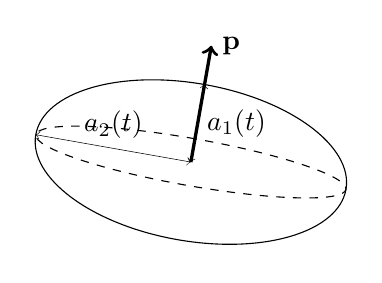
\begin{tikzpicture}[rotate=80]
        \draw(0,0) ellipse (1 cm and 2 cm);
        \draw[dashed](0,0) ellipse (0.3 cm and 2 cm);
        \draw[<->,very thin](0,0) --++ (1,0)node[midway,right]{$a_1(t)$};
        \draw[->,very thick](0,0) --++ (1.5,0)node[right]{$\textbf{p}$};
        \draw[<->,very thin](0,0) --++ (0,2)node[midway,above]{$a_2(t)$};
    \end{tikzpicture}
    \hfill
    \caption{Scheme of an  oblate spheroid oriented along the unit vector \textbf{p} with $a_1(t)$ and $a_2(t)$ the length of the semi axes of the spheroid.
    Note that when the drop is spherical we have $a_1=a_2=a$}
    \label{fig:scheme_spheroid}
\end{figure}
This shape might be described completely by the second moment of mass, $\textbf{M}_\alpha$.
In this context, each eigenvalue of the second moment of mass tensor is proportional to square semi axes of the particle. 
Indeed, by direct integration over the spheroidal particle volume we may find :
\begin{equation*}
    \textbf{M}_\alpha
    = \frac{m_\alpha a^2}{5}\left[
        \left(\frac{a_1}{a}\right)^2\textbf{pp}
        + \left(\frac{a_2}{a}\right)^2 (\textbf{I} - \textbf{pp}),
    \right] 
\end{equation*}
Additionally, note that due to the volume conservation condition we have : $ a_2^2 a_1 = a^3$. 
This means that : $M_1 = M_2^{-2}$, where the $M_i$ are the eigenvalues of the dimensionless tensor $\frac{m_\alpha a^2}{5}\textbf{M}_\alpha^* = \textbf{M}_\alpha$. 
Note that if we consider small deformations, meaning $M_1 - 1 \ll 1$ we have $M_1  = M_2^{-2} = 1 - 2 (M_2 - 1) + \mathcal{O}((M_2 -1)^2)$. 
Consequently, for small deformation the trace of the second moment of mass tensor reads :  $\frac{1}{3}\textbf{I}:\textbf{M}_\alpha = M_1 + 2M_2 = 1 - 2M_2 + 2M_2 = 1$. 
Therefore in the limit of small deformation the droplet shape is completely determined by one scalar value $M_1$ or $M_2$, and the orientation tensor $\textbf{p}$. 

Additionally, with this definition we can introduce the distance function  $\FF_\alpha$. 
It reads, 
\begin{equation*}
    \FF_\alpha(\textbf{x},t) = \textbf{rr}:\textbf{M}_\alpha^* -a^2.  
    \label{eq:distance_function}
\end{equation*}
The point on the surface of the particle are defined through $\FF_\alpha(\textbf{x}_I,t) = 0$. 
Being able to define the droplet's shape in such a rigorous way will find its use in the calculation of the surface tension stress. 
Using these definition makes the dimensionless  second moment of mass the same as the Cauchy green deformation tensor. 

\subsubsection*{The droplet's internal velocity}


We know that an isolated droplet in creeping flow with translating motion exhibit internal motion known as Hill vortexes, see \ref{fig:flowlines} (b). 
For a drop immersed in an unbounded linear flow, still in stokes flows, we can derive an analytical solution such that $\textbf{w}_2^0 \sim \textbf{rrr}$, see \ref{fig:flowlines} (a). 
If slightly more inertial effects are present one might find that the internal motion are close to hill's vortexes but with an overall oblate spheroidal shape, see \ref{fig:flowlines} (c). 
In these cases the droplet's internal velocity fields is a steady solution.
Nevertheless, for a droplet to go from case (b) to case (c) a deformation must occur. 

To account for this deformation in our case we assume that the secondary velocity field that is responsible for the deformation is purely a linear function of the position. 
The internal velocity field of a particle under homogeneous linear deformation can be described as such, $\textbf{w}_2^0 = \bm\Gamma_\alpha \cdot \textbf{r}$. 
We have introduced, $\bm\Gamma_\alpha$, the mean velocity gradient inside the particle, which symmetric part : $\textbf{E}_\alpha$, represents the rate of strain, and skew symmetric part : $\bm\Omega_\alpha$, represents the angular velocity. 

\begin{figure*}
    \centering
    \begin{tikzpicture}
        \node (img3) at (0.6\textwidth,0) {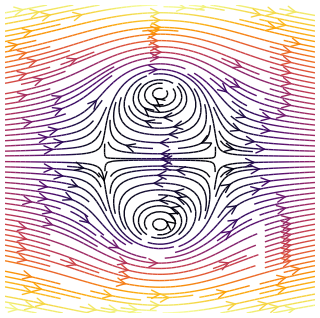
\includegraphics[width=0.3\textwidth,angle=270]{image/Rising_def_Stokes.png}};
        \node (img2) at (0.3\textwidth,0) {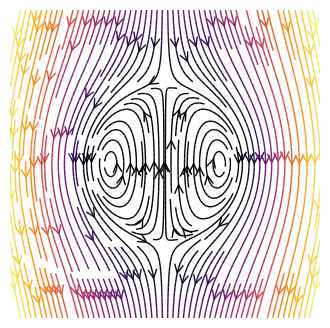
\includegraphics[width=0.3\textwidth]{image/Rising_Stokes.png}};
        % \draw (0.45\textwidth,0)node{$\rightarrow$};
        % \draw (0.45\textwidth,0.4cm)node{$\bm\Gamma_\alpha\cdot \textbf{r}$};
        \node (img1) at (0.0\textwidth,0) {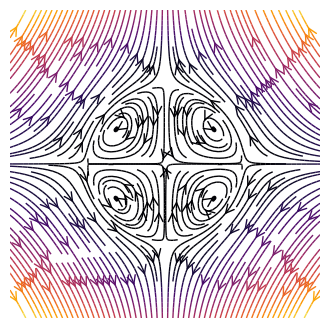
\includegraphics[width=0.3\textwidth]{image/Shear_Stokes.png}};
        \draw (img3.south)node{(c)};
        \draw (img2.south)node{(b)};
        \draw (img1.south)node{(a)};
    \end{tikzpicture}
    \caption{Three examples of steady state flow lines plots of an isolated droplet immersed into a viscous fluid. 
    (a) Rising sphere in uniform stokes flow (analytical solution in \ref{ap:Translating_sphere}). 
    (b) Fixed droplet in extensional flow (analytical solution in \ref{ap:Translating_sphere}).
    (c) Deformed droplet in rising motion (analytical solution of \citet{taylor1964deformation}). }
    \label{fig:flowlines}
\end{figure*}
To summarize, we assume that the inner velocity field of the drop can be decomposed into two distinct part. 
The first one is the steady state component, examples are : hill's vortex for spherical and oblate spheroidal drop in steady linear motion, the inner velocity field of a drop in steady linear flows, and so on. 
The second contribution is the inner velocity fields that alter the drop's shape, this field is assumed linear with the position and homogeneous, that is $\bm\Gamma\cdot \textbf{r}$. 
Adopting these definitions, the particle internal velocity is written, 
\begin{equation}
    \textbf{w}_{2,i}^0(\textbf{x}_\alpha)
    = \bm\Gamma_{\alpha,ik}(t) \cdot \textbf{r}_k
    + \textbf{w}^{s}_{2,i}(t,\textbf{r})
    =\bm{\Omega}_{\alpha,ik}\cdot \textbf{r}_k
    + \textbf{E}_{\alpha,ik} \cdot \textbf{r}_k
    + \textbf{w}^{s}_{2,i}(t,\textbf{r})
    \label{eq:def_vel}
\end{equation}
Where we introduced the vector $\textbf{w}^{s}_2(t,\textbf{r}) =\textbf{w}^{0}_{2,i}(t,\textbf{r})  - \bm\Gamma_{\alpha,ik}(t) \cdot \textbf{r}_k$ which represents all the internal motions that does not alter the drop's shape. 

An important consequence of this definition is that the integral on the RHS of \ref{eq:dt_S_alpha} is null when $\textbf{w}_{2,i}^0 = \textbf{w}_{2,i}^s$. 
This can be shown by re writting the second moment of mass equation with the use of the velocity decomposition.
This yields,
\begin{equation*}
    \ddt \textbf{M}_{\alpha,ik}
    = 
    \textbf{M}_{\alpha,ik} \cdot \bm\Gamma_{\alpha,kj}
    +  \bm\Gamma_{\alpha,ki} \cdot \textbf{M}_{\alpha,jk}
    +
    \intO{ 
        \textbf{w}_{2,i}^s\textbf{r}_j
        + \textbf{r}_i\textbf{w}_{2,j}^s
    }
\end{equation*}
In the cases where $\bm\Gamma = 0$, the droplet shape remains steady, in this case $\ddt \textbf{M}_\alpha = 0$ and $\intO{\textbf{w}^{s}_{2,i} \textbf{r}_j + \textbf{r}_i \textbf{w}_{2,i}^s} = 0$. 
In the case where $\bm\Gamma \neq 0$ the droplets deform according to the linear velocity fields $\bm\Gamma\cdot \textbf{r}$.
Since we assumed that no other source of deformation are present than the latter, we must have $\intO{\textbf{w}^{s}_{2,i} \textbf{r}_j + \textbf{r}_i \textbf{w}_{2,i}^s} = 0$ so that $\textbf{w}^{s}_{2,i} $ doesn't contribute to the deformation nor the rotation.
This, means that $\textbf{w}^{s}_{2,i}$ is a velocity fields determined in  part by the instantaneous shape of the droplet and its , that does not alter the shape of the drop. 
Additionally, the angular momentum is assumed to be entirely described by $\textbf{M}_\alpha \cdot \bm\Omega_\alpha$ meaning that, $\textbf{r} \textbf{w}_{2}^s$ plays no role at all in the total particle's moment of momentum.
This type of velocity fields is encountered in linear skew symmetric flows where the rotation is homogeneous and follow the carrier fluid vorticity. 
Anyhow, this velocity decomposition has the plaisent property that $\textbf{P}_\alpha = \bm\Gamma \cdot \textbf{M}_\alpha + \intO{\textbf{w}^{s}_{2,i} \textbf{r}_j} =  \bm\Gamma \cdot \textbf{M}_\alpha $ at all time, which will simplify the equaitons of motions. 

Now some constrain should apply on the tensor $\textbf{E}_\alpha$.
Indeed, the mass conservation inside the particle \ref{eq:dt_rho} impose $\div \textbf{u}_2^0 = \textbf{E}_\alpha : \textbf{I}= 0$, where it is assumed that $\div \textbf{w}_2^s =0$. 
Also, note that to preserve the spheroidal shape of the particle we must assume that the particle's rate of strain principal direction is the same as the droplet's shape principal axis. 
In other worlds, $\textbf{E}_\alpha$ must have the same eigenbasis as $\textbf{M}_\alpha$. 
Making up with these two constrain leads to the expression : $\textbf{E}_\alpha = -2 E_2 \textbf{pp} + E_2 (\textbf{I}- \textbf{pp})$, where $E_2$ is the second eigenvalue of $\textbf{E}_\alpha$. 


As it is demonstrated in \ref{ap:Translating_sphere} the internal motion of an isolated spherical drop, such as the one in \ref{eq:def_vel}, is entirely determined  from $\textbf{u}_1$,$\grad\textbf{u}_1$,$\textbf{u}_\alpha$ and so on. 
Therefore, it is reasonable to think that in a more general case, $\textbf{w}_2^s$ might be entirely determined by the carrier fluid and particles' properties, namely, $\textbf{u}_\alpha$ $\textbf{M}_\alpha$, $\textbf{u}_1$ $\grad\textbf{u}_1$ and for non-dilute flows we might have $\phi_2$ or more complicated functions. 
Thus, from now on we consider that the internal velocity $\textbf{w}^{s}_2(t,\textbf{r})$ is not part of the particle' unknown, but rather is a closure term. 
Consequently, in this problem a single droplet is described exhaustively by, $\textbf{x}_\alpha, \textbf{u}_\alpha, \textbf{M}_\alpha$ and $\bm\Gamma_\alpha$. 
This requires two additional equations one for $\textbf{M}_\alpha$ and another for $\bm\Gamma_\alpha$. 

\subsubsection*{The conservation equations}

The integrals appearing in \ref{eq:dt_M_alpha} and \ref{eq:dt_P_alpha} can be reformulated using the previous decomposition of the internal velocity field, and it reads, 
\begin{align}
    \intO{(\textbf{rw}_ 2^0 )_{ij}+ (\textbf{w}_2^0 \textbf{r})_{ij}} 
    = \textbf{M}_{\alpha,ik} \cdot \bm\Gamma_{\alpha,jk}
        +  \bm\Gamma_{\alpha,ik} \cdot \textbf{M}_{\alpha,jk}
    \\
    \intO{\rho_2 \textbf{w}_{2,i}^0\textbf{w}_{2,j}^0}
    = \bm\Gamma_{\alpha,jl}\bm\Gamma_{\alpha,ik} \textbf{M}_{\alpha,kl}  
        +\intO{\rho_2 \textbf{w}_{2,i}^s\textbf{w}_{2,j}^s}
    \\
    \intO{\bm\sigma_{2,ij}^0}
    =
    2 \mu_2 v_\alpha \textbf{E}_{\alpha,ij}
    - \intO{p_2^0} \textbf{I}_{ij}
    + \mu_2 \intS{(\textbf{n}_i \textbf{w}_{2,j}^s + \textbf{n}_j \textbf{w}_{2,i}^s)}
    \\
    \intS{\bm\sigma_{I,ij}^0}
    = \frac{\gamma v_\alpha }{a} \left[
        2\textbf{I}_{ij} 
        - \frac{4  }{5} (\textbf{M}_{\alpha,ij}^* - \textbf{I}_{\alpha,ij})
    \right]
    +\mathcal(O)((\textbf{M}_\alpha-\textbf{I})^2)\\
    % s_\alpha 
    % = 4\pi a^2 (1+\frac{\textbf{M}:\textbf{M}}{15})
\end{align}
The reformulation of the moment of momentum have already been treated above. 
The surface tension stress has been derived in the limit of small deformation. 
Note that our formula agree with the one derived by \citet{lhuillier1987phenomenology}. 
The detailed calculation of the surface tension stress tensor is given in appendix. 
We provide the exact results as well as the Taylor expansion of this formula for small deformation. 

Injecting these formulas inside \ref{eq:dt_M_alpha} and \ref{eq:dt_P_alpha} yields an equation for the deformation and the rate of strain of the drop. 
If we separate the skew-symmetric, symmetric and trace of the moment of momentum equation we obtain and equation for $\bm\Omega_\alpha$ and one fer  $\textbf E_\alpha$, namely,
\begin{align*}
    % \ddt \textbf{pp}_{\alpha,ij}
    % = \textbf{pp}_{\alpha,ik} \cdot \bm\Omega_{\alpha,jk}
    % +  \bm\Omega_{\alpha,ik} \cdot \textbf{pp}_{\alpha,jk}\\
    \ddt \textbf{M}_{\alpha,ij}
    = \textbf{M}_{\alpha,ik} \cdot \bm\Gamma_{\alpha,jk}
    +  \bm\Gamma_{\alpha,ik} \cdot \textbf{M}_{\alpha,jk}\\
    \ddt (\textbf{I}_{\alpha,ik}\bm\omega_{\alpha,k} )
    = 
    \intS{(\textbf{r}\times\bm\sigma_1^0\cdot \textbf{n})_i} \\
    \frac{1}{2}\ddt^2 \textbf{M}_{\alpha,ij}
    -  \bm\Gamma_{\alpha,jl}\bm\Gamma_{\alpha,ik} \textbf{M}_{\alpha,kl}  
    + \mu_2 v_\alpha 2\textbf{E}_{\alpha,ij}
    + \frac{\gamma v_\alpha }{a} \left[
    2\textbf{I}_{ij} 
    - \frac{4 }{5} (\textbf{M}_{\alpha,ij}^* - \textbf{I}_{\alpha,ij})
    \right]\\
    = 
    \frac{1}{2}\intS{(\textbf{r}\bm\sigma_1^0 + \bm\sigma_1^0\textbf{r})\cdot \textbf{n}} 
    + \intO{\rho_2 \textbf{w}_{2,i}^s\textbf{w}_{2,j}^s}
    + \intO{p_2^0} \textbf{I}_{ij}
    - \mu_2 \intS{(\textbf{n}_i \textbf{w}_{2,j}^s + \textbf{n}_j \textbf{w}_{2,i}^s)}\\
    % \frac{1}{2}\ddt^2 \textbf{M}_{\alpha,mm}
    % -  \bm\Gamma_{\alpha,ml}\bm\Gamma_{\alpha,mk} \textbf{M}_{\alpha,kl}  
    % + \frac{\gamma v_\alpha }{a} 
    % \left[
    % 2\textbf{I}_{mm} 
    % % - \frac{4 }{5 } (\textbf{M}_{\alpha,mm}^* - \textbf{I}_{\alpha,mm})
    % \right]
    % = 
    % \intS{\textbf{r}_m\cdot\bm\sigma_{1,mk}^0\cdot \textbf{n}_k} 
    % + \intO{\rho_2 \textbf{w}_{2,m}^s\cdot \textbf{w}_{2,m}^s}
    % + \intO{p_2^0} \textbf{I}_{mm}
\end{align*}
The second moment of mass \ref{eq:dt_Cs}, is consistent with the equation found by \citet{goddard1967nonlinear} and \citet{lhuillier1987phenomenology}. 
Following, \citet{goddard1967nonlinear}  terminology, the left-hand side of \ref{eq:dt_Cs} is referred as the \textit{convected} derivative of $\textbf{M}^*_\alpha$. 
Therefore, the \textit{convected} derivative of $\textbf{M}_\alpha$ is equal to the rate of strain of the particle. 
The skew-symmetric part of the first moment of momentum \ref{eq:dt2_C}, it is basically the angular momentum balance of a non-spherical object. 
The right-hands side accounting for the external torque contribution. 
The symmetric part however has the form of a non-linear forced harmonic oscillatory equation for the droplet deformation. 
Indeed, the first groups of terms on the left-hand side represent the inertial contribution of the droplet internal fluid. 
It is made of a second order derivative plus non-linear terms in $\bm\Gamma_\alpha$. 
The second groups of terms is internal viscous contribution that arise directly from the definition of the stress \ref{eq:sigma_2_def}. 
It vanishes for small viscosity ration and is linear in the first derivative of $\textbf{M}_\alpha$. 
The last term on the left-hand side is the elastic response from the interface which is negligible for high capillary number $Ca \to \infty$. 
Then on right-hand side of the equation we find the first moment of surface force, $\intS{(\textbf{r}\bm\sigma_1^0+ \bm\sigma_1^0\textbf{r})\cdot \textbf{n}}^*$ which has an unknown expression at this stage. 
\ref{eq:dt2_C} might be regarded as a second order harmonic equation with non-linear contributions. 
However, the unknown integrals $\intO{\rho_2 \textbf{w}_{2,i}^s\textbf{w}_{2,j}^s},
\intS{(\textbf{n}_i \textbf{w}_{2,j}^s + \textbf{n}_j \textbf{w}_{2,i}^s)}$ and $\intS{(\textbf{r}\bm\sigma_1^0+ \bm\sigma_1^0\textbf{r})\cdot \textbf{n}}^*$ are in general function of the shape of the particle so on $\textbf{M}_\alpha$ and its higher derivatives of $\textbf{M}_\alpha$.
These terms have to be seen as forcing terms. 
Therefore, at this stage it is impossible to predict the nature of the harmonic regime followed by the droplet. 
To conclude on this matter one must find an expression for all this closure as well as determinate the impact of the non-linear terms.



We now focus on the rate of strain equation. 
To better understand this equation we introduce the following dimensionless groups, 
\begin{align*}
    \intO{\rho_2 \textbf{w}_{2,i}^0\textbf{w}_{2,j}^0}
    \sim \frac{m_\alpha a^2}{\tau_u^2} \textbf{F}_{ww}^*
    \\
    - \intO{p_2^0\textbf{I}}
    + \mu_2 \intS{(\textbf{n}_i \textbf{w}_{2,j}^s + \textbf{n}_j \textbf{w}_{2,i}^s)}
    \sim \frac{v_\alpha \mu_2}{\tau_u} \textbf{F}_{e}^*
    \\
    \intS{\textbf r \bm\sigma_1^0 \cdot \textbf{n}}
    \sim 
    \frac{v_\alpha \mu_1}{\tau_u} \textbf{F}_{\sigma}^*
\end{align*} 
where we have assumed that the internal and external stress contribution followed a viscous scaling. 
The time $\tau_u$ represent the external solicitation time-scale. 
Which is in opposition to the droplets rate of strain and rotation time scale such that $\bm\Gamma = 1/\tau \bm\Gamma^*$. 
\begin{align*}
    \frac{\zeta Re}{5}\left[
        \beta^2 \frac{1}{2}\ddt^2 \textbf{M}_{\alpha,ij}
    -   \beta^2 \bm\Gamma_{\alpha,jl}\bm\Gamma_{\alpha,ik} \textbf{M}_{\alpha,kl}  
    - \textbf{F}_{ww}^*
    \right]
    + \lambda  \left[
        \beta 2\textbf{E}_{\alpha,ij}
    +  \textbf{F}_\sigma^*
    \right]
    + \frac{1}{Ca} \left[
    2\textbf{I}_{ij} 
    - \frac{4  }{5} (\textbf{M}_{\alpha,ij}^* - \textbf{I}_{\alpha,ij})
    \right]
    = 
    \frac{1}{2}
    \textbf{F}_{\sigma_1}^*
    % \intS{(\textbf{r}\bm\sigma_1^0 + \bm\sigma_1^0\textbf{r})\cdot \textbf{n}} 
    % + \intO{p_2^0} \textbf{I}_{ij}
\end{align*}
where we have defined the following dimensionless groups : 
\begin{align*}
    \beta = \frac{\tau_u}{\tau}
    && \zeta = \rho_2 /\rho_1
    && \lambda = \mu_1/\mu_2 
    && Re = \frac{\rho_1 a^2 }{ \mu_1 \tau_u}
    && Ca = \frac{a \mu_1}{\gamma \tau_u}
\end{align*}

We now examine the specific case studied by \citet{lamb1924hydrodynamics} where he considered no external contribution around the particle nor rotational motion.
Also, it is considered that the deformation within the particle are linear and small. 
Keeping only the trace of this equation yields the low deformation system of equation :
\begin{align*}
    \ddt \textbf{M}_{\alpha,ij} = \textbf{E}_{\alpha,ij}\\
    \frac{\zeta Re}{5}
        \beta^2 \frac{1}{2}\ddt^2 \textbf{M}_{\alpha,ij}
    % -   \beta^2 \bm\Gamma_{\alpha,jl}\bm\Gamma_{\alpha,ik} \textbf{M}_{\alpha,kl}  
    % - \textbf{F}_{ww}^*
    % \right]
    + \lambda 
        \beta 2\textbf{E}_{\alpha,ij}
    % +  \textbf{F}_\sigma^*
    % \right]
    - \frac{1}{Ca} 
     \frac{4  }{5} (\textbf{M}_{\alpha,ij}^* - \textbf{I}_{\alpha,ij})
    = 0
    % \frac{1}{2}
    % \textbf{F}_{\sigma_1}^*
    % \intS{(\textbf{r}\bm\sigma_1^0 + \bm\sigma_1^0\textbf{r})\cdot \textbf{n}} 
    % + \intO{p_2^0} \textbf{I}_{ij}
\end{align*}
Notice that this is a second order oscillatory equation. 
This is equivalent to  \citet{lamb1924hydrodynamics}. 
Therefore our model is somewhat more general. 

Lastly, as it will be usefull for latter let consider the cases wheer the timescale of the flow is much smaller that the one of the particle rate of strain, in this case $\beta \ll 1$. 
Making use of this fact makes the moment of momentum equation as, 
\begin{align*}
    - \frac{\zeta Re}{5}
     \textbf{F}_{ww}^*
    + \lambda  
    \textbf{F}_\sigma^*
    + \frac{1}{Ca} \left[
    2\textbf{I}_{ij} 
    + \frac{4  }{5} (\textbf{M}_{\alpha,ij}^* - \textbf{I}_{\alpha,ij})
    \right]
    = 
    \frac{1}{2}
    \textbf{F}_{\sigma_1}^*
    % \intS{(\textbf{r}\bm\sigma_1^0 + \bm\sigma_1^0\textbf{r})\cdot \textbf{n}} 
    % + \intO{p_2^0} \textbf{I}_{ij}
\end{align*}
This is the steady state equilibrium equation of the first moment of force. 
If the capillary number is low enough the last term  completely balance the external stress. 

% 
\subsection{From Lagrangian to Eulerian fields}

Up to this point, we have described the dispersed phase within a Lagrangian framework.
However, to be consistent with the Eulerian conservation equations used to describe the continuous phase, we need to extend the Lagrangian equations to an Eulerian models. 
In order to achieve this, we introduce the function $\delta_\alpha$, which is defined as follows, 
\begin{align}
    \delta_\alpha(\textbf{x},t) = \delta(\textbf{x}-\textbf{x}_\alpha(t,\FF)).
    \label{eq:delta_alpha}
\end{align}
where $\delta$ is the Dirac delta function.
Note that we explicitly note $\textbf{x}_\alpha(t,\FF)$ since the posiiton of the particle $\alpha$ is function of time and of the flow configuration $\FF$.
In the sens of generalized functions, the partial time derivative, $\pddt \delta_\alpha(\textbf{x},t,\FF) =  \frac{\partial \textbf{x}_\alpha}{\partial t} \cdot \grad_{\textbf{x}_\alpha} \delta_\alpha$ can be re-written into the following expression, 
\begin{equation}
    \pddt \delta_\alpha
    + \div (\textbf{u}_\alpha  \delta_\alpha)
    =0,
    \label{eq:dt_delta_alpha}
\end{equation}
where we used the identity, $\grad_{\textbf{x}_\alpha} \delta_\alpha = -\grad \delta_\alpha$ and the fact that $\textbf{u}_\alpha(t;\FF)$ is not a function of $\textbf{x}$. 
Additionally, it should be noted that \ref{eq:dt_delta_alpha} is not applicable if changes in topology, such as break up or coalescence events, occur.
In such cases it is possible, as it is done in population balance equations, to include a source term on the RHS of \ref{eq:dt_delta_alpha} to account for particle birth or death. 
Multiplying each Lagrangian quantities by $\delta_\alpha$ yields the \textit{particle field} of a quantity $q_\alpha$, denoted as $q_\alpha(t)\delta_\alpha(\textbf{x},t)$, which is defined throughout space and time.
Likewise, for any derivative of Lagrangian quantities, such as $\ddt q_\alpha$, we define its corresponding Eulerian field by Multiplying $\ddt q_\alpha$ with $\delta_\alpha$ and show that :
\begin{equation}
    \delta_\alpha \ddt q_\alpha
    = \pddt (\delta_\alpha q_\alpha)
    + \div (\delta_\alpha q_\alpha \textbf{u}_\alpha)
    \label{eq:dt_delta_alpha_q_alpha}
\end{equation}
where we have utilized the fact that $q_\alpha(t)$ and $\textbf{u}_\alpha(t)$ are solely functions of time, and we made use of \ref{eq:dt_delta_alpha}.
Additionally, let's consider a volume containing $N$ particles.
We can then define the particle-field of a given quantity $q_\alpha$ as the sum of all the independent field, i.e. $\sum_{\alpha=0}^N \delta_\alpha q_\alpha$.
Notice that \ref{eq:dt_delta_alpha_q_alpha} remains valid for a sum of fields since derivative operators are linear.
To simplify the notations, we consider implicitly the summation over all particles included in $\Omega$ whenever a Lagrangian field denoted by $\delta_\alpha (\ldots)$ is present.

Multiplying \ref{eq:dt_q_alpha_tot} and \ref{eq:dt_Q_alpha_tot} by $\delta_\alpha$, summing over all particles, and by considering \ref{eq:dt_delta_alpha_q_alpha}, it is straightforward to show that,
\begin{equation}
    \pddt (\delta_\alpha  q_\alpha^\text{tot})
    + \div (\delta_\alpha\textbf{u}_\alpha q_\alpha^\text{tot})
    = \delta_\alpha\intO{ s_2^0 }
    + \delta_\alpha\intS{ s_I^0 }
    + \delta_\alpha\intS{ \left[\mathbf{\Phi}_1^0 + f_1^0 (\textbf{u}_I^0-\textbf{u}_1^0) \right] \cdot \textbf{n}_2 },
    \label{eq:dt_dq_alpha_tot}
\end{equation}
\begin{multline}
    \pddt (\delta_\alpha  \mathcal{Q}_\alpha^\text{tot})
    + \div (\delta_\alpha\textbf{u}_\alpha \mathcal{Q}_\alpha^\text{tot})
    = \delta_\alpha\intO{ \left(
        \textbf{r} s_2^0         
        + f_2^0  \textbf{w}_2^0 
        - \mathbf{\Phi}_2^0
    \right) }\\
    + \delta_\alpha\intS{ \left(
        \textbf{r}s_I^0
        + f_I^0 \textbf{w}_I^0
        - \mathbf{\Phi}_{||I}^0
    \right) }
    + \delta_\alpha\intS{ \textbf{r} \left[
        \mathbf{\Phi}_1^0
        + f_1^0 (\textbf{u}_I^0-\textbf{u}_1^0)
    \right]\cdot \textbf{n}_2  }.
    \label{eq:dt_dQ_alpha_tot}
\end{multline}
Similar consideration can be applied to the higher order moments equations derived in \ref{ap:moment_derivative}.

At this stage, we obtained two sets of equations that can be used to describe the dispersed phase. 
The first set of equations is the global conservation laws, i.e. \ref{eq:dt_chi_k_f_k} with for $k=2$ and \ref{eq:dt_delta_I_f_I}. 
The other is the particle-fields equations, such as \ref{eq:dt_dq_alpha_tot} and potentially the higher moments equations.
Therefore, some comments are in order regarding the differences and compatibility of these two sets of equations.
Solving \ref{eq:dt_dq_alpha_tot} ideally provides us with a field $\delta_\alpha(q_\alpha+q_{I\alpha})$ which contains the Lagrangian properties $q_\alpha+q_{I\alpha}$.
Thus, it corresponds to the volume and surface integral of $f_2^0$ and $f_I^0$ on $\Omega_\alpha$ and $\Sigma_\alpha$ respectively.
While, in \ref{eq:dt_chi_k_f_k} we solve the equation for the complete field $f_2^0$ defined inside the domains $\Omega_\alpha$.  
Thus, from  \ref{eq:dt_f_k} to \ref{eq:avg_dt_dq_alpha_tot} we lose the detailed description of $f_2^0$ within the particles' domain.
Indeed, with \ref{eq:avg_dt_dq_alpha_tot}, we recover solely the integrated value of $f_2^0$ over the particles' volume and surface. 
Therefore, \ref{eq:dt_dq_alpha_tot} can be though as averaged equations of \ref{eq:dt_chi_k_f_k} and \ref{eq:dt_delta_I_f_I} since we recover only the integrated properties of each particle. 
It is important to understand that in this sense, the passage from \ref{eq:dt_chi_k_f_k} and \ref{eq:dt_delta_I_f_I} to \ref{eq:dt_dq_alpha_tot} is an average operation carried out on the particles' volume and surface.
Likewise, \ref{eq:dt_dQ_alpha_tot} is an equation for the first moment of the distribution of $f_2^0$ and $f_I^0$ within the particle's volume and surface.

% Note that this is different to the usual averaged technics that refer to the ones used to derive the classic averaged models such as in \citet{jackson1997locally} and \citet{zhang1994averaged}.
% which are the subject of the following section. 


\section{The hybrid model}
\label{sec:averaged_eq}
\tb{expose the avg equaiton under the form of the particles phase exposed above }
\tb{ Maybe do the local reference frame avg eq }
\tb{ Explain that these need closure and that the kinetic internal eq can be used for the shape as well }
\tb{ Then the form of some closure is derived in appendix }
% 
% \subsection{Phase average and particle averaged equations}
% Correspondingly, we take the average of the particle fields equations by using \ref{eq:avg} on \ref{eq:dt_dq_alpha_tot} and \ref{eq:dt_dQ_alpha_tot}, which gives, 
In the objective of obtaining coarse-grained level equations for the dispersed phase, one must apply an ensemble average operator on \ref{eq:avg_dt_dq_alpha_tot} and \ref{eq:avg_dt_dQ_alpha_tot} which is made possible since the particle fields $\delta_\alpha \ldots$ are now defined over the whole space $\Omega$ thanks to the Dirac delta functions $\delta_\alpha$.  
These equations yields,
\begin{align}
    \pddt \avg{\delta_\alpha  q_\alpha^\text{tot}}
    + \div \avg{\delta_\alpha\textbf{u}_\alpha q_\alpha^\text{tot}}
    &= \pOavg{ s_2^0 }
    + \pSavg{ s_I^0 }
    + \pSavg{ \left[\mathbf{\Phi}_1^0 + f_1^0 (\textbf{u}_I^0-\textbf{u}_1^0) \right] \cdot \textbf{n}_2 ,}
    \label{eq:avg_dt_dq_alpha_tot}\\
    \pddt \avg{\delta_\alpha \mathcal{Q}_\alpha^\text{tot}}
    + \div \avg{\delta_\alpha\textbf{u}_\alpha\mathcal{Q}_\alpha^\text{tot}}
    &=\pOavg{ \left(
        \textbf{r} s_2^0         
        + f_2^0  \textbf{w}_2^0 
        - \mathbf{\Phi}_2^0
    \right) }
    + \pSavg{ \left(
        \textbf{r}s_I^0
        + f_I^0 \textbf{w}_I^0
        - \mathbf{\Phi}_{I||}^0
    \right) }\nonumber\\
    &+ \pSavg{ \textbf{r} \left[
        \mathbf{\Phi}_1^0
        + f_1^0 (\textbf{u}_I^0-\textbf{u}_1^0)
    \right]\cdot \textbf{n}_2  }.
    \label{eq:avg_dt_dQ_alpha_tot}
\end{align}
In \ref{ap:Moments_equations} the derivation of the higher moment particle-averaged equations is provided. 
In this study,\ref{eq:avg_dt_chi_f} and \ref{eq:avg_dt_delta_f} are refereed to as the phase-averaged equations, while \ref{eq:avg_dt_dq_alpha_tot} and \ref{eq:avg_dt_dQ_alpha_tot} are denoted as the particle-averaged equation. 
In these expressions we kept a general notation yet. 
But note that, we can note the particle phase averaged quantity by,
\begin{equation}
     n_p q_p(\textbf{x},t) = \avg{\delta_\alpha q_\alpha}
     \label{eq:p_avg}
\end{equation}
where, $n_p(\textbf{x},t) = \avg{\delta_\alpha}$ is the probable number of finding a particle center of mass at $\textbf{x}$
and $q_p$ is the conditional average of $q_\alpha$ conditionally on the presence of a particle at \textbf{x}. 
Additionally, notice that it is possible to define the fluctuating parts of a property by, 
\begin{equation}
    q_\alpha' = q_\alpha - q_p
    % \;\;\;\;\;\;\text{and}
    % \;\;\;\;\;\;
\end{equation}
such that the particle average of a product can be rewritten, $\pavg{q_\alpha\textbf{u}_\alpha} = n_p q_p \textbf{u}_p + \pavg{q_\alpha' \textbf{u}_\alpha'}$. 
These notations will find their use in \ref{sec:averaged_eq}, but for now we keep the formulation rather generic as in \ref{eq:avg_dt_dQ_alpha_tot} and \ref{eq:avg_dt_dq_alpha_tot}

As remarked by \citet{jackson1997locally} for the angular momentum equations of solid spherical particles, and here in a more general case :\ref{eq:avg_dt_chi_f} and \ref{eq:avg_dt_dq_alpha_tot} may seem to be not coupled with the higher order moments equations, i.e. \ref{eq:avg_dt_dQ_alpha_tot}. 
Indeed, the first order moment $\mathcal{Q}_p^\text{tot}$ do not appear explicitly in either \ref{eq:avg_dt_chi_f} or \ref{eq:avg_dt_dq_alpha_tot}.
However, the exchange and source terms 
appearing in both \ref{eq:avg_dt_chi_f} and \ref{eq:avg_dt_dQ_alpha_tot} might depend on the higher order moments of the particles.
Indeed, in the momentum equation of the continuous phase, i.e. the ensemble average of \ref{eq:dt_rhou_k}, the exchange term corresponds to the averaged drag force, namely $\pSavg{\bm{\sigma}_1^0\cdot \textbf{n}_2}$. 
It is clear that $\pSavg{\bm{\sigma}_1^0\cdot \textbf{n}_2}$ has a strong dependency with $\textbf{u}_p$,$\mathcal{P}_p$ and $\mathcal{M}_p$ since the drag force is a function of both the particle's kinematic and its shape. 
Therefore, \ref{eq:avg_dt_dQ_alpha_tot} is linked to \ref{eq:avg_dt_chi_f} and \ref{eq:avg_dt_dq_alpha_tot} solely through the dependence of the exchange and source terms with the properties of the particles, e.g. $q_p,\mathcal{Q}_p$ and possibly the higher order moments. 
This reasoning applies for the energy equation and all kinds of conservation equation. 
Ultimately, the significance of the higher moments equations can be evaluated based on the dependency of the closure terms present in \ref{eq:avg_dt_chi_f} with the properties of the particle : $q_p, \mathcal{Q}_p$ and potentially the higher-order moments of the particles. 


% 
%\subsubsection*{Equivalence between particle and continuous models}
\subsection{Equivalence between particle-averaged and phase-averaged equations}
\label{sec:equivalence}
To model the dispersed phase we can either use \ref{eq:avg_dt_chi_f} with $k=2$, or the particle-average \ref{eq:avg_dt_dq_alpha_tot}, \ref{eq:avg_dt_dQ_alpha_tot} and possibly the higher moments equations. 
As mentioned in \ref{sec:Lagrangian} we notified that \ref{eq:dt_dq_alpha_tot} was already subject to an average over the particles' volume and the surfaces. 
Meaning that \ref{eq:avg_dt_dq_alpha_tot} is the results of two average processes. 
Consequently, it is fair to address the question of the compatibility and differences between both formalism, i.e. between \ref{eq:avg_dt_chi_f} and \ref{eq:avg_dt_dq_alpha_tot}. 

To begin with, it has been demonstrated in various studies \citep{nott2011suspension,jackson1997locally,zhang1994averaged}, that phase-averaged quantities can be expressed as a Taylor series expansion of particle-averaged quantities. 
Indeed, the dispersed phase indicator function $\chi_2(\textbf{x},t)$ can be expressed as a sum of phase indicator function, $\chi_2(\textbf{x},t) = \sum_\alpha\chi_\alpha(\textbf{x},t)$ where $\chi_\alpha =1$ in the particle domain $\Omega_\alpha(t)$ and $0$ otherwise. 
Then, notice that any a dispersed phase quantity can be written as, 
\begin{equation*}
    f^0_2 \chi_2(\textbf{x},t)
    = \sum_\alpha f^0_2 \chi_\alpha(\textbf{x},t) 
    = \sum_\alpha \int_{\mathbb{R}^3} f^0_2 \chi_\alpha(\textbf{x}_\alpha+\textbf{r},t)\delta(\textbf{x}- \textbf{x}_\alpha - \textbf{r}) d\textbf{r} 
\end{equation*}
Which upon using the Taylor expansion of the Dirac delta function in the neighborhood of $\textbf{r}=0$ one obtain :  $\delta(\textbf{x}- \textbf{x}_\alpha - \textbf{r}) = \delta(\textbf{x}- \textbf{x}_\alpha) - \textbf{r}\cdot\grad \delta(\textbf{x} - \textbf{x}_\alpha) + \frac{\textbf{rr}}{2}:\grad\grad\delta(\textbf{x}- \textbf{x}_\alpha)\ldots $.
% Thus, the dispersed phase quantity $(f_2^0\chi_2)$ can be re-written as, 
% \begin{equation*}
%     f^0_2 \chi_2(\textbf{x},t)
%     = \sum_\alpha \left[
%         \intO{f^0_2}
%         - \div\intO{\textbf{r} f^0_2}
%         + \frac{1}{2}\grad\grad :\intO{\textbf{rr} f^0_2}
%         \ldots
%     \right]
% \end{equation*}
% where we recognize the zeroth, first and second order moments of $f_2^0$. 
Applying these considerations to interfaces quantities and averaging over all configurations of the phase space, one obtain a general relation between continuous and particle averaged quantities, namely, 
\begin{align}
    \avg{\chi_2f_2^0} 
    &=  \pavg{q_\alpha}
        - \div  
        \pavg{\mathcal{Q}_\alpha}        
        + \frac{1}{2} \grad\grad : \pavg{\mathcal{Q}_{2\alpha}}
        + \ldots  
        \nonumber\\
    \avg{\delta_I f_I^0} 
    &=  \pavg{q_{I\alpha}}        
        - \div \pavg{\mathcal{Q}_{I\alpha}}
        + \frac{1}{2} \grad\grad : \pavg{\mathcal{Q}_{I\alpha}^{2}}
        + \ldots  
    \label{eq:f_exp}
\end{align}
It must be noted that \ref{eq:f_exp} is the bridge between the continuous phase average formalism and the particle formulation. 
One of the consequences of these relations is that, 
\begin{align}
    \phi_2 \rho_2
    = m_p n_p 
    + \frac{1}{2}\grad^2 : (n_p\mathcal{M}_p)+\ldots\\
    \phi_2 \rho_2 \textbf{u}_2
    = m_p n_p \textbf{u}_p 
    - \div (n_p\mathcal{P}_p)+\ldots
    \label{eq:f_exp_exe}
\end{align}
meaning that $\phi_2\rho_2$ is in fact related to $\mathcal{M}_p$ and the phase averaged velocity $\textbf{u}_2$ contain the first  moment of momentum $\mathcal{P}_p$, which account for rotational and stretching motions of the particles. 

In order to establish the equivalence between both formalism, we follow the strategy of \citep{lhuillier2000bilan,lhuillier2009rheology} by taking the Taylor expansion of each terms in \ref{eq:avg_dt_chi_f} with $k=2$ using the relation \ref{eq:f_exp}. 
Since we made use of the surface transport equations in the particles phase equations : \ref{eq:avg_dt_dq_alpha_tot} and \ref{eq:avg_dt_dQ_alpha_tot}, we also need to consider \ref{eq:avg_dt_delta_f}  to prove equivalence. 
As the resulting expression can become quite cumbersome, we will adopt the following definition. 
Let $\mathbb{C}_2$ represent the phase-averaged equation of conservation (\ref{eq:avg_dt_chi_f} with $k=2$) and $\mathbb{C}_I$ the averaged surface transport equation, namely, 
\begin{align*}
    \mathbb{C}_2
    &=
    - \pddt \avg{\chi_2f_2^0}
    - \div \avg{\chi_2 \mathbf{\Phi}_2^0 - \chi_2f_2^0 \textbf{u}_2^0}
    + \avg{\chi_2 s_2^0}
    + \avg{\delta_I\left[
        \mathbf{\Phi}_2^0
        + f_2^0
        \left(
            \textbf{u}_I^0
            - \textbf{u}_2^0
        \right)
    \right]
    \cdot \textbf{n}_2}.\\
    \mathbb{C}_I
    &= 
    -\pddt \avg{\delta_If_I^0}
    -\div \avg{\delta_I f_I^0 \textbf{u}_I^0-\delta_I \mathbf{\Phi}_{I||}^0 }
    + \avg{\delta_Is_I^0} 
    - \avg{\delta_I \Jump{
    f_k^0 (\textbf{u}_I^0 - \textbf{u}_k^0)
    + \mathbf{\Phi}_k^0
    } }. 
\end{align*}
It must be understood from \ref{eq:avg_dt_chi_f} and \ref{eq:avg_dt_delta_f} that $\mathbb{C}_2=0$ and $\mathbb{C}_I=0$.
Then, by taking the Taylor expansion of each terms of $\mathbb{C}_2+\mathbb{C}_I$ according to \ref{eq:f_exp}, we can equally show that,
\begin{equation}
    \mathbb{C}_2 
    + \mathbb{C}_I 
    = \mathbb{M}_0 - \div \mathbb{M}_1 + \frac{1}{2} \grad\grad : \mathbb{M}_2 \ldots = 0,
    \label{eq:scheme_equivalence}
\end{equation} 
where the expression $\mathbb{M}_0$ and $\mathbb{M}_1$ turn out to be, 
\begin{align*}
    &\mathbb{M}_0
    = 
    - \avg{\delta_\alpha \ddt {q_\alpha^\text{tot}}}
    % -\avg{\delta_\alpha\textbf{u}_\alpha q_\alpha^\text{tot}}
    + \pOavg{ s_2^0 }
    + \pSavg{ s_I^0 }
    + \pSavg{ 
    \left[\mathbf{\Phi}_1^0 
    + f_1^0 (\textbf{u}_I^0-\textbf{u}_1^0) \right] \cdot \textbf{n}_2 },\\
    &\mathbb{M}_1 =
    -  \avg{\delta_\alpha \ddt {\mathcal{Q}_\alpha^\text{tot}}}
    % - \avg{\delta_\alpha\textbf{u}_\alpha \mathcal{Q}_\alpha^\text{tot}}
     + \pOavg{ \left(
        \textbf{r} s_2^0         
        + f_2^0  \textbf{w}_2^0 
        - \mathbf{\Phi}_2^0
    \right) }
    + \pSavg{ \left(
        \textbf{r}s_I^0
        + f_I^0 \textbf{w}_I^0
        - \mathbf{\Phi}_{I||}^0
    \right) }\\
    &+ \pSavg{ \textbf{r} \left[
        \mathbf{\Phi}_1^0
        + f_1^0 (\textbf{u}_I^0-\textbf{u}_1^0)
    \right]\cdot \textbf{n}_2  },
\end{align*}
respectively. 
In the presence of \ref{eq:scheme_equivalence} we reach the major conclusion of this work. 
Indeed, we can observe that $\mathbb{M}_0$, $\mathbb{M}_1$ and $\mathbb{M}_2$ represent the zeroth, first and second order moments equations, respectively. 
In fact, it is shown in \ref{ap:Moments_equations} that the coefficient $\mathbb{M}_n$ in \ref{eq:scheme_equivalence} correspond to the $n^{th}$ order particle-average conservation equation. 
As a matter of fact, the phase average applied to the dispersed phase contains all the particle-averaged moments equations.
In \ref{ap:Moments_equations} we provide the expression for each moment equation $\mathbb{M}_n$ as well as the complete derivation of \ref{eq:scheme_equivalence}. 
In \cite{lhuillier2000bilan} they reached similar conclusion when comparing the area density phase-averaged and particle-averaged equations of conservation for spherical particles. 
Thus, from \ref{eq:scheme_equivalence} it is evident that one can use an arbitrary order of moments equations to reach an arbitrary accurate description of the dispersed phase.

Another approach is to notice that $\mathbb{M}_n=0$ for all $n$. Thus, we can rewrite \ref{eq:scheme_equivalence} such that all moments equations vanish, except $\mathbb{M}_0$, which gives, 
\begin{equation}
    \mathbb{C}_2 = \mathbb{M}_0 = 0.
\end{equation}
This implies that equation \ref{eq:avg_dt_chi_f} with the surface transport equation \ref{eq:avg_dt_delta_f} is rigorously equivalent to \ref{eq:avg_dt_dq_alpha_tot} which has been shown by \cite[Appendix A]{nott2011suspension} for the specific case of the momentum conservation equation of solid spherical particle.
In fact, we generalize the conclusion of \citet[Appendix A]{zhang1997momentum} which stipulate that the particle momentum equation is as legitimate as the phase averaged equation. 
In fact, it is not surprising at all, since the phases and particles averaged equations are all constructed from \ref{eq:dt_f_k}.
However, if one do not consider a proper derivation as it is done in \ref{sec:Lagrangian} it might not be as obvious, even if it should remain.
Nevertheless, it is important to note that this conclusion is not entirely objective since following the same procedure we could show equally that $\mathbb{C}_2  = -\div\mathbb{M}_1=0$ and $\mathbb{C}_2  = \frac{1}{2}\grad\grad:\mathbb{M}_2=0$ and so on for the other higher terms. 
Thus, it is more appropriate to examine the problem from the perspective of \ref{eq:scheme_equivalence}. 
Namely, the particle-averaged equations constitute a system of equations with one equation for each moment, while the phase-averaged equation contains all the terms of the particle-averaged equations within a single equation.
Therefore, the particle-averaged formalism encompasses more information since it provide one equation for each moment. 
This,  gain in information have been possible through the consideration of the topology of the dispersed phase. 

The major consequence of this finding is that it enable us to better understand the role of the particle phase stresses $\phi_2\bm{\sigma}_2$ and $\phi_I\bm{\sigma}_I$, in the particle averaged momentum equation such as it is written in a kinetic-like model. 
Indeed, as shown by the general form \ref{eq:avg_dt_dq_alpha_tot}, $\phi_2\bm{\sigma}_2$ and $\phi_I\bm{\sigma}_I$ will not play a role on the particle averaged momentum equations, i.e. the equation of : $n_p m_p \textbf{u}_p$. 
However, as shown in \ref{eq:dt_avg_uk2}, the phase averaged momentum : $\rho_2 \phi_2 \textbf{u}_2$,  will be subject to the particle surface and internal stresses, since $\phi_2\bm{\sigma}_2$ and $\phi_I\bm{\sigma}_I$ are present in this phase averaged equation.
This is made consistent if one consider that these stresses act as source terms on the higher moments of momentum equations $\mathbb{M}_1$\ldots, which are related to $\rho_2 \phi_2 \textbf{u}_2$ through \ref{eq:f_exp_exe}. 
In brief, the non-convective fluxes $\phi_2\bm{\sigma}_2$ and $\phi_I\bm{\sigma}_I$  have no direct impact on the particle averaged center of mass momentum :$n_pm_p\textbf{u}_p$, regardless of the particles nature and volume fraction. 
The influence of $\phi_2\bm{\sigma}_2$ and $\phi_I\bm{\sigma}_I$ on the particles' averaged momentum, $n_p m_p \textbf{u}_p$ is made through the dependence of the source terms present in \ref{eq:avg_dt_dq_alpha_tot} with the higher moments of the particles, which depend themselves on the non-convective fluxes as suggested by the moments of momentum equations. 
Consequently, it must be understood that the kinetic-like equations are formally exact and apply for any type of particle and particle volume fraction, as long as the closure terms are well modeled. 
Similar remarks can be made regrading the non-convective fluxes of the energy equation $\textbf{q}_2$ and for all other conservation equation. 



% 

\subsection{The bulk stress in dispersed multiphase flow}



Now that the architecture of the averaged dispersed multiphase flow equation is clarified, we would like to present the expression of the bulk stress tensor in a suspension of inertial particles subject to an arbitrary local body force field, $\textbf{b}^0$.
Firstly, is important to recall the definition of the \textit{bulk stress}. 
We define the \textit{bulk stress} tensor as a force applied on the fluid and on the particles phase, having the form $\div \bm{\Sigma}$, which added to the total external force $\textbf{B}$, balance exactly the material derivative of the mixture momentum : $\frac{D \rho \textbf{u}}{Dt}$. 
In this definition $\textbf{B}$ cannot be decomposed into a vector and a divergence of a tensor, in which case the latter would just contribute to $\bm{\Sigma}$.

We first expose the averaged mixture momentum and angular momentum equation easily derived from \ref{eq:dt_avg_f}, 
\begin{align}
    \pddt (\rho u_i)
    + \partial (\rho u_iu_k
    + \sigma_{ik}^\text{eq})
    = b_i\\
    \epsilon_{ijk} \sigma_{jk}
    = 0 
    \label{eq:momentum_bulk}
\end{align}
In the momentum equation we have defined, $\sigma_{ik}^\text{eq} = \avg{\rho\textbf{u}'\textbf{u}'}
- \avg{\chi_1\bm{\sigma}_1^0}-\avg{\chi_2\bm{\sigma}_2^0} - \avg{\delta_I \bm{\sigma}_I^0}$. 
Additionally, in the averaged angular momentum equation we have assumed that no-body torque exist at the local scale making the second equality equal to $0$ \citet{leal2007advanced} and the averaged mixture stress $\bm{\sigma}$ a symmetric quantity. 
However, note that $\bm{\sigma}$ is not exactly equal to the \textit{bulk stress} tensor $\bm{\Sigma}$ since $\textbf{b}$ can be expressed as a divergence of a stress.
Indeed, have defined $\textbf{b} = \textbf{B} + \div  \pMOavg{\textbf{b}_2^0}$ where $\textbf{B} = \phi_1 \textbf{b}_1 +  \pOavg{\textbf{b}_2^0 }$ and  $\pMOavg{\textbf{r}\textbf{b}_2^0}$ is defined accordingly to the previous definition. 
It follows the definition of the \textit{bulk stress} : 
\begin{equation}
    \bm{\Sigma}
    = 
    \avg{\rho\textbf{u}'\textbf{u}'}
    - \avg{\chi_1\bm{\sigma}_1^0}
    - \avg{\chi_2\bm{\sigma}_2^0} 
    - \avg{\delta_I \bm{\sigma}_I^0}
    - \pMOavg{\textbf{r}\textbf{b}_2^0}
\end{equation}
which proves already, in the absence of particles moments of the body forces $\pMOavg{\textbf{r}\textbf{b}_2^0}$, the antisymmetric part of the suspension stress is null, in agreement with \citet{dolata2020heterogeneous}.
% This skew symmetric part can be written in vector form as, 
% \begin{equation*}
%     \epsilon_{ijk}\textbf{T}_{jk}
%     = 
%     -\epsilon_{ijk} \pOavg{r_kb_j}
%     -\epsilon_{ijk}\frac{1}{2}\partial_l \pOavg{r_lr_kb_j}
%     = 0  
% \end{equation*}
We recall that the carrier fluid is a Newtonian fluid, therefore we may express the fluid phase stress as, 
\begin{equation}
    \phi_1 \sigma_{1,jk}
    = -p_1 \delta_{jk}
    + \mu_1 e_{jk}
    - \mu_1 \phi_2 e_{2,jk}. 
\end{equation} 
Additionally, we use the methodology of \citep{lhuillier1992volume,lhuillier1996contribution} to re express the averaged particle stress terms. 
The divergence of the particle phase stress may be expressed using \ref{eq:f_exp}, 
\begin{align}
    \label{eq:exp_sigma22}
    \partial_k \avg{\chi_2 {\sigma}_2^0}_{ik}
    &=  \partial_k\pOavg{ {\sigma}_{2,ik}^0}
    -\frac{1}{2} \partial_k\partial_j
    \pOavg{ r_j{\sigma}^0_{2,ik} + r_k\sigma^0_{2,ij}}
    + \ldots  \\
    \label{eq:exp_sigmaI2}
    \partial_k \avg{\delta_I {\sigma}^0_I}_{ik} 
    &=  \partial_k\pSavg{ {\sigma}_{I,ik}^0 }
        -\frac{1}{2} \partial_k\partial_j \pSavg{ r_j {\sigma}_{I,ik}^0+r_k {\sigma}_{I,ij}^0 }
        + \ldots  
\end{align}
Note that the heterogeneous terms must remain symmetric in the index $kj$ due to the double contraction with the operator $\partial_k\partial_j$, thus only the symmetric part in $jk$ remain and the terms such as, $\pOavg{ r_j{\sigma}^0_{2,ik} - r_k\sigma^0_{2,ij}}$ vanish. 
Upon the use of the moment of momentum equation of the first and second order we can easily derive these expressions, 
\begin{align}
    \intS{ (\bm{\sigma}_I)_{ik}}
    +\intO{ (\bm{\sigma}_2^0)_{ik}}
    = 
    \intO{ \rho_2 
    (\textbf{w}_2^0\textbf{w}_2^0  )_{ik}
    }
    -\ddt \intO{ r_i (\textbf{u}^0_2)_k }
    +\intS{ 
        b_{i}
        r_k 
    }
    +\intS{ 
     r_i (\bm{\sigma}_1^0 \cdot \textbf{n}_2)_{k}
    }
    \label{eq:dt_P_alpha}\\
    \intO{ r_{j}(\bm{\sigma}^0_2)_{ik}+r_{k}(\bm{\sigma}^0_2)_{ji}}
    +\intS{ r_{j}(\bm{\sigma}^0_I)_{ik}+r_{k}(\bm{\sigma}_I^0)_{ji}}
    = 
    - \ddt\intO{ \rho_2 (\textbf{u}_2^0)_i r_j r_k }\nonumber\\
    + \intO{ \rho_2 (r_{j} (\textbf{w}_2^0)_k (\textbf{u}^0_2)_i + r_k (\textbf{w}_2^0)_j (\textbf{u}^0_2)_i)}
    +\intS{  r_{k}r_{j} (\bm{\sigma}_1^0)_{il} (\textbf{n}_2)_l }
    + \intO{ r_{k}r_{j}  \rho_2 b_i } 
    \label{eq:dt_P2_alpha}
\end{align}
It is evident that by using an arbitrary order of moment of momentum equation one can substitute any volume integral of the particle stress appearing in the expansion \ref{eq:exp_sigma22}. 
% By consideration of symmetric of the local stress, it is evident that the skew symmetric part of the moment of momentum will not have any dynamical role thus we can retrieve the average of \ref{eq:dt_mu_alpha} to the first relation. 
% To extract the skew symmetric part we start by writing the permutation of these equations with $ik$ yielding,  
% \begin{align}
%     \intS{ 
%     (\bm{\sigma}_I)_{ki}
%     }
%     +\intO{ 
%     (\bm{\sigma}_2^0)_{ki}
%     }
%     = 
%     \intO{ \rho_2 
%     (\textbf{w}_2^0\textbf{w}_2^0  )_{ki}
%     }
%     -\ddt \intO{ r_k (\textbf{u}^0_2)_i }
%     +\intS{ b_{k}r_i }
%     +\intS{ r_k (\bm{\sigma}_1^0 \cdot \textbf{n}_2)_{i}}\\
%     \intO{ r_{j}(\bm{\sigma}^0_2)_{ki}+r_{i}(\bm{\sigma}^0_2)_{jk}}
%     +\intS{ r_{j}(\bm{\sigma}^0_I)_{ki}+r_{i}(\bm{\sigma}_I^0)_{jk}}
%     = 
%     - \ddt\intO{ \rho_2 (\textbf{u}_2^0)_k r_j r_i }\nonumber\\
%     + \intO{ \rho_2 (r_{j} (\textbf{w}_2^0)_i (\textbf{u}^0_2)_k + r_i (\textbf{w}_2^0)_j (\textbf{u}^0_2)_k)}
%     +\intS{  r_{i}r_{j} (\bm{\sigma}_1^0)_{kl} (\textbf{n}_2)_l }
%     + \intO{ r_{i}r_{j}  \rho_2 b_k } \\
%     \intO{ r_{i}(\bm{\sigma}^0_2)_{jk}+r_{k}(\bm{\sigma}^0_2)_{ij}}
%     +\intS{ r_{i}(\bm{\sigma}^0_I)_{jk}+r_{k}(\bm{\sigma}_I^0)_{ij}}
%     = 
%     - \ddt\intO{ \rho_2 (\textbf{u}_2^0)_j r_i r_k }\nonumber\\
%     + \intO{ \rho_2 (r_{i} (\textbf{w}_2^0)_k (\textbf{u}^0_2)_j 
%     + r_k (\textbf{w}_2^0)_i (\textbf{u}^0_2)_j)}
%     +\intS{  r_{k}r_{i} (\bm{\sigma}_1^0)_{jl} (\textbf{n}_2)_l }
%     + \intO{ r_{k}r_{i}  \rho_2 b_j } 
% \end{align}
% Acknowledgement of the symmetrical nature of $\bm{\sigma}_2^0$ and $\bm{\sigma}_I^0$ gives the following antisymmetrical balance equations, 
% \begin{align}
%     0
%     = 
%     -\ddt \intO{ r_i (\textbf{u}^0_2)_k -r_k (\textbf{u}^0_2)_i }
%     +\intS{ b_{i}r_k -b_{k}r_i }
%     +\intS{r_i (\bm{\sigma}_1^0 \cdot \textbf{n}_2)_{k} - r_k (\bm{\sigma}_1^0 \cdot \textbf{n}_2)_{i}}\\
%     \intO{ r_{j}(\bm{\sigma}^0_2)_{ik}
%             -r_{i}(\bm{\sigma}^0_2)_{jk}}
%     +\intS{ r_{j}(\bm{\sigma}^0_I)_{ik}
%            - r_{i}(\bm{\sigma}_I^0)_{jk}}
%     = 
%     - \ddt\intO{ \rho_2 (\textbf{u}_2^0)_i r_j r_k -  \rho_2 (\textbf{u}_2^0)_j r_i r_k }\nonumber\\
%     + \intO{ \rho_2 (r_{j} (\textbf{w}_2^0)_k (\textbf{u}^0_2)_i + r_k (\textbf{w}_2^0)_j (\textbf{u}^0_2)_i)}
%     - \intO{ \rho_2 (r_{i} (\textbf{w}_2^0)_k (\textbf{u}^0_2)_j + r_k (\textbf{w}_2^0)_i (\textbf{u}^0_2)_j)}\\
%     +\intS{  r_{k}r_{j} (\bm{\sigma}_1^0)_{il} (\textbf{n}_2)_l 
%     -r_{k}r_{i} (\bm{\sigma}_1^0)_{jl} (\textbf{n}_2)_l }
%     + \intO{ r_{k}r_{j}  \rho_2 b_i
%     - r_{k}r_{i}  \rho_2 b_j } 
% \end{align}
% The last equation need to be added to the second permutation which gives, 
% \begin{align*}
% \intO{ r_{j}(\bm{\sigma}^0_2)_{ik}}
% +\intS{ r_{j}(\bm{\sigma}^0_I)_{ik}}
% = 
% - \ddt\intO{ \rho_2 (\textbf{u}_2^0)_k r_j r_i 
% + \rho_2 (\textbf{u}_2^0)_i r_j r_k 
% -  \rho_2 (\textbf{u}_2^0)_j r_i r_k }\nonumber\\
% + \intO{ \rho_2 (r_{j} (\textbf{w}_2^0)_k (\textbf{u}^0_2)_i + r_k (\textbf{w}_2^0)_j (\textbf{u}^0_2)_i)}
% - \intO{ \rho_2 (r_{i} (\textbf{w}_2^0)_k (\textbf{u}^0_2)_j + r_k (\textbf{w}_2^0)_i (\textbf{u}^0_2)_j)}\\
% - \intO{ \rho_2 (r_{j} (\textbf{w}_2^0)_i (\textbf{u}^0_2)_k + r_i (\textbf{w}_2^0)_j (\textbf{u}^0_2)_k)}\\
% +\intS{  r_{k}r_{j} (\bm{\sigma}_1^0)_{il} (\textbf{n}_2)_l 
% +r_{j}r_{i} (\bm{\sigma}_1^0)_{kl} (\textbf{n}_2)_l 
% -r_{k}r_{i} (\bm{\sigma}_1^0)_{jl} (\textbf{n}_2)_l }
% + \intO{ r_{k}r_{j}  \rho_2 b_i
% + r_{j}r_{i}  \rho_2 b_k 
% - r_{k}r_{i}  \rho_2 b_j 
% } 
% \end{align*}
In, addition one must notice that the particle angular momentum balance equation doesn't involve the integral of the particle local stress and has therefore, no dynamical role in the equivalent stress expression. 
Making use of these remarks we obtain this general formula for the suspension stress,  
\begin{multline}
    \bm{\Sigma}
    = \avg{\rho\textbf{u}'\textbf{u}'}_{ik}
    + \phi_1 p_1 \delta_{ik}
    - \mu_1 e_{ik}
    % + \mu_1 \phi_2 e_{2,ik}. 
    - \pOavg{ \rho_2 (\textbf{w}_2^0\textbf{w}_2^0  )_{ik}}
    + \pavg{\ddt {\mathcal{S}_{ik}} }\\
    - \pSavg{ b_{i}r_k - b_{k}r_i }
    - \pSavg{ r_i (\bm{\sigma}_1^0 \cdot \textbf{n}_2)_{k}
    + r_k (\bm{\sigma}_1^0 \cdot \textbf{n}_2)_{i}}
    + \mu_1 \pOavg{e_2^0}_{ik}
    + \frac{1}{2} \div\bm{\Sigma}_1
    \label{eq:eq_stress}
\end{multline}
with the inhomogeneous stress gathered in $\bm{\Sigma}_1$, namely,
\begin{multline}
    \bm{\Sigma}_1
    = 
    - \pavg{\ddt\intO{ \rho_2 (\textbf{u}_2^0)_i r_j r_k }}
    + \pOavg{ \rho_2 (r_{j} (\textbf{w}_2^0)_k (\textbf{u}^0_2)_i + r_k (\textbf{w}_2^0)_j (\textbf{u}^0_2)_i)}\nonumber\\
    +\pSavg{  r_{k}r_{j} (\bm{\sigma}_1^0)_{il} (\textbf{n}_2)_l }
    - \mu_1 2 \pOavg{\textbf{r} \textbf{e}_2^0}_{jik}
\end{multline}
According to \ref{eq:scheme_equivalence}, expanding each component related to the dispersed phase in \ref{eq:momentum_bulk} one would see appear each moment of momentum equations under the divergence operator.
However, to stay consistent with the definition of the bulk stress tensor $\bm{\Sigma}$, we must keep the advecting term on the LHS of \ref{eq:momentum_bulk} unchanged, this is however not the case of the averaged body force term $\textbf{b}$ which allowed us to cancel all the body forces terms with the expansion of $\textbf{T}$.  

One of the major question in suspension dynamic raised by several authors, is the evaluation of the bulk stress or equivalent stress tensor of a suspension, see \citep{prosperetti2006stress, batchelor1970stress,zhang1997momentum,nadim1996concise} and more recently \citet{dolata2020heterogeneous}. 
The answer to this question is given in the general case of the generic averaged mixture equation. 
In light of \ref{eq:eq_stress} we have demonstrated how to express in a routine manner the bulk stress of the particle phase. 
And doing so without making appear explicitly the particles  internal stress. 
This, conclusion deserve several comments regarding previous studies. 
In  \citet{jackson1997locally},  the volume averaged momentum balance (equation (38) of \citet{jackson1997locally}) they make appear the higher moment of velocity of the particles as closure terms, these are hidden in $\pOavg{\textbf{w}_2^0 \textbf{w}_2^0}$.
However, in \citet{jackson1997locally} they did not remove the angular momentum to the stress yieldings a slightly different term. 
What we have shown here is that these higher moments of the particles phase such has the particles rotations have no dynamical significance in the mixture equations. 
Therefore, equation (38) of \citet{jackson1997locally} can be further simplified to the fluid and first order particle averaged equations. 
Equally, in the momentum mixture equation derived by \citet{zhang1997momentum} (equation (8.2)), they make appear explicitly the higher moment of acceleration and the higher moments of velocity in their equivalent stress. 
These terms must therefore simplify. 
In fact as, it could be supposed in their appendix these moments equally cancel. 
In agreement with \citet{dolata2021faxen} which also found that the only remaining part of the stress were solely the fluid phase exchange terms upon the calculation of the body forces moments. 
Similar, comments can be made on the study of \citet{prosperetti2006stress}. 
This also explain why \citet{nadim1996concise} found out that the interfacial terms of the surface tension and viscous interfacial forces play no direct role in the equivalent stress of the emulsion.
% 
Now that we reached a clear understanding of the mathematical structures of the averaged two phase flow equation we start to expose the averaged set of equations which constitute the \textit{Hybrid model}. 
As, mentioned in \ref{sec:two-fluid} we consider the mass, momentum and energy for the particles and continuous phase. 
Additionally, to describe higher degree of freedom of the particle shape and momentum, one must consider the second moment of mass and first moment of momentum averaged equations. 
This, makes a total of 10 equations, 6 for the particle phase and 4 for the continuous phase.
This system involves numerous equations and closures terms, it is therefore important to consider in a second step a routine to simplify this system by the consideration of the physical particle degree of freedom.
This; is the subject of the next section.    

\subsection{Continuous phase equations}

\tb{peut etre mettre les terme du second ordre}
The equations for the carrier are basically the same as in the classic to fluid model except that the interfacial terms must be modified in order to have the same form as the dispersed phase equations \citep{jackson1997locally,zhang1994averaged}. 
It is done through the use of \ref{eq:f_exp} which help us to convert the exchange terms of the form of $\avg{\delta_I \ldots }$ appearing in \ref{eq:avg_dt_chi_f} to a series expansion of particle phase  quantity : $\pSavg{\ldots} - \div (\ldots)$. 
Where the first term of this series corresponding to the particle averaged equations exchange term. 
Note that due to the expansion shape of \ref{eq:f_exp} we also see appear higher moments of surface in the fluid phase equations, they will be responsible for the additional fluxes in the fluid phase equation due to the presence particles. 
We start by exposing the . 
The continuous phase primary equations simply derived using the generic expression : \ref{eq:avg_dt_chi_f}, and applying the preceding remarks to the interfacial term. 
The mass, momentum and total energy of the continuous phase yield, 
\begin{align}
    \label{eq:dt_hybrid_rho}
    &\pddt (\phi_1 \rho_1)  
    + \div (
        \phi_1 \rho_1\textbf{u}_1
    )
    = 
    0\\
    \label{eq:dt_hybrid_rhou_1}
    &\pddt (\phi_1 \rho_1\textbf{u}_1)  
    + \div (
        \phi_1 \rho_1\textbf{u}_1\textbf{u}_1
        + \bm{\sigma}_1^\text{eq}
    )
    = 
    \phi_1 \rho_1 \textbf{g} 
    - \pSavg{{\bm{\sigma}_1^0 \cdot \textbf{n}_2}}
    % +\div  \pSavg{{\textbf{r}\bm{\sigma}_1^0 \cdot \textbf{n}_2}}
    \\
    \label{eq:dt_hybrid_rhoE_1}
    &\pddt (\phi_1\rho_1E_1)  
    + \div (
        \phi_1\rho_1E_1\textbf{u}_1
        + \bm{q}_1^\text{eq}
        + \textbf{u}_1 \cdot \bm{\sigma}_1^\text{eq}
        % - \textbf{u}_1^0 \cdot \bm{\sigma}_1^0 
        % + \textbf{q}_1^0
        )
    = 
    \phi_1 \rho_1\textbf{u}_1 \cdot \textbf{g} 
    - \textbf{u}_p \cdot \pSavg{{\bm{\sigma}_1^0 \cdot \textbf{n}_2}}\nonumber \\
    &- \pavg{ \textbf{u}_\alpha' \cdot \intS{  \bm{\sigma}_1^0 \cdot \textbf{n}_2}}
    - \pavg{ \intS{\textbf{w}_2^0 \cdot \bm{\sigma}_1^0 \cdot \textbf{n}_2}}
    + \pSavg{{\textbf{q}_1\cdot \textbf{n}_2}}
    % &\div [    
        % \textbf{u}_p \cdot \pSavg{{ \textbf{r}\bm{\sigma}_1^0 \cdot \textbf{n}_2}}
    % + \pavg{ \textbf{u}_\alpha' \cdot \intS{ \textbf{r} \bm{\sigma}_1^0 \cdot \textbf{n}_2}}
    % + \pavg{ \intS{\textbf{r}\textbf{w}_2^0 \cdot \bm{\sigma}_1^0 \cdot \textbf{n}_2}}
    % - \pavg{ \intS{\textbf{r}  \textbf{q}_1^0 \cdot \textbf{n}_2}}
    % ]
\end{align} 
where we defined the equivalent stress tensor $\bm{\sigma}_1^\text{eq}$ and energy flux $\textbf{q}^\text{eq}_1$ as,
\begin{align}
    \label{eq:sigma_eq_def}
    \bm{\sigma}_1^\text{eq}
    =& 
    \avg{\chi_1\rho_1\textbf{u}_1'\textbf{u}_1'}
    - \phi_1 \bm{\sigma}_1%- n_p \textbf{M}_p
    - \pSavg{{\textbf{r}\bm{\sigma}_1^0 \cdot \textbf{n}_2}}\\
    \textbf{q}_1^\text{eq}
    =&\textbf{q}_1^\text{e} +\textbf{q}_1^\text{k}  \nonumber\\
    \textbf{q}_1^\text{e}
    =& \rho_1 \avg{\chi_1 \textbf{u}_1' e_1'} 
    + \phi_1\textbf{q}_1 
    +\pSavg{{\textbf{r}\textbf{q}_1^0 \cdot \textbf{n}_2}} 
    \nonumber\\
    \textbf{q}_1^\text{k}
    =& \rho_1 \avg{\chi_1 \textbf{u}_1' k_1} 
    - \avg{\chi_1 \textbf{u}_1' \cdot \bm{\sigma}_1^0}
    + (\textbf{u}_1 - \textbf{u}_p)\cdot
    \pSavg{{\textbf{r}\bm{\sigma}_1^0 \cdot \textbf{n}_2}}
    \nonumber\\\nonumber
    &- \pavg{ \textbf{u}_\alpha' \cdot \intS{ \textbf{r} \bm{\sigma}_1^0 \cdot \textbf{n}_2}}
    - \pavg{ \intS{\textbf{r}\textbf{w}_2^0 \cdot \bm{\sigma}_1^0 \cdot \textbf{n}_2}}
\end{align}
It is clear that those equations yield essentially the same as the previous set of equations presented in \ref{sec:two-fluid}.
The only difference is the presence of additional fluxes inside $\bm{\sigma}^\text{eq}_1$ and $\textbf{q}^\text{eq}_1$. 
Especially, one can remark the presence of the first moments of external forces. 
In facts, according to \ref{eq:f_exp} an infinite number of moments is present however we chose to explicit only the first of the series. 

% \tb{introduce the exchange term explain the drag and first moments here, just recall that we already seen them}
% \tb{Insiste on the fact that this formulation is physical and NEW}
In this form of the averaged momentum equation we see appear the terms $\pSavg{\bm{\sigma}_1^0 \cdot \textbf{n}_2}$ which is the total components of the interphase drag force, including the mean pressure gradient of the fluid phase pressure. 
Likewise, $\pSavg{\textbf{r}\bm{\sigma}_1^0 \cdot \textbf{n}_2}$ is the total averaged first moment of force traction, which include the mean fluid phase pressure $p_1$. 
As discussed in \ref{sec:Lagrangian} this terms symmetric and skew symmetric part represent the averaged stresslet and torque on the particles, respectively.  
The latter is responsible for the Einstein viscosity computed in dilute stokes flow regime \citep{guazzelli2011}. 
The exchange term in \ref{eq:dt_avg_rhoE_k} have been decomposed into three exchange terms.
Indeed, after taking the Taylor expansion of $\avg{\delta_I (\textbf{u}^0_2 \cdot \bm{\sigma}_1^0 \cdot \textbf{n}_2)}$  we used the following decomposition on each of the moments :
\begin{align}
    \label{eq:exergysource}
    \pavg{ \intS{\textbf{u}^0_2 \cdot \bm{\sigma}_1^0 \cdot \textbf{n}_2}}
    &= 
    \textbf{u}_p \cdot \pSavg{{\bm{\sigma}_1^0 \cdot \textbf{n}_2}}
    + \pavg{ \textbf{u}_\alpha' \cdot \intS{  \bm{\sigma}_1^0 \cdot \textbf{n}_2}}
    + \pavg{ \intS{\textbf{w}_2^0 \cdot \bm{\sigma}_1^0 \cdot \textbf{n}_2}}\\
    \pavg{ \intS{\textbf{r}\textbf{u}^0_2 \cdot \bm{\sigma}_1^0 \cdot \textbf{n}_2}}
   &= 
    \textbf{u}_p \cdot \pSavg{{\bm{\sigma}_1^0 \cdot \textbf{n}_2}}
    + \pavg{ \textbf{u}_\alpha' \cdot \intS{\textbf{r}  \bm{\sigma}_1^0 \cdot \textbf{n}_2}}
    + \pavg{ \intS{\textbf{r}\textbf{w}_2^0 \cdot \bm{\sigma}_1^0 \cdot \textbf{n}_2}}
\end{align}
In this form the contribution to the energy exchange is now clear. 
The first term on the right hands side of \ref{eq:exergysource} represents the work done by the mean phase relative motion, the second term is the work made by the resultants of the forces and individual particles fluctuating velocity, the last term represent the work made by the local force traction on the particle surface with the surface velocity relative to the particle center of mass velocity.
Same comments can be made for the first order moments. 
The relative importance of these three contribution will be determined in the next section, especially we will see that  it depends highly on the particles' nature. 
To our knowledge, such a decomposition has not been seen in the literature except in \citep[Chapter 2]{scorsim2021particle} where they make similar consideration, but for solid spherical particles.
% It is mainly due to the facts that these equations are often used in the context of two-phase flow modeling, which disregard the equation of the dispersed phase energy. 
We recall that the stress integral $\pSavg{\bm{\sigma}_1^0 \cdot \textbf{n}_2}$ contains contact forces as well, making our model consistent with the latter study. 

As discussed previously, \ref{eq:dt_avg_uk2}, \ref{eq:dt_avg_kk} and \ref{eq:dt_avg_ek} need to be reformulated consistently with the dispersed phase exchange term. 
The mean kinetic energy, pseudo turbulent energy and internal energy equation can be reformulated as, 
\begin{align}
    \pddt (\phi_1 \rho_1u_1^2/2)  
    + \div (
        \phi_1 \rho_1\textbf{u}_1u_1^2/2
        + \textbf{u}_1 \cdot \bm{\sigma}_1^\text{eq}
    )
    = 
     \bm{\sigma}_1^\text{eq} : \grad \textbf{u}_1
    + \phi_1 \rho_1 \textbf{u}_1\cdot \textbf{g} 
    -  \textbf{u}_1\cdot 
        \pSavg{{\bm{\sigma}_1^0 \cdot \textbf{n}_2}} 
        % - \div 
        % \pSavg{{\textbf{r}\bm{\sigma}_1^0 \cdot \textbf{n}_2}} 
        \\
    \label{eq:dt_hybrid_k1}
    \pddt (\phi_1\rho_1k_1)  
    + \div (
        \phi_1\rho_1k_1\textbf{u}_1
        + \textbf{q}_1^\text{k} 
        )
    = 
    - \avg{\chi_1\bm{\sigma}_1^0 : \grad \textbf{u}_1^0}
    - \bm{\sigma}_1^\text{eq} : \grad \textbf{u}_1\nonumber
    - \pavg{ \textbf{u}_\alpha' \cdot \intS{  \bm{\sigma}_1^0 \cdot \textbf{n}_2}}\\
    + (\textbf{u}_1 - \textbf{u}_p)\cdot \pSavg{{\bm{\sigma}_1^0 \cdot \textbf{n}_2}} 
    - \pavg{ \intS{\textbf{w}_2^0 \cdot \bm{\sigma}_1^0 \cdot \textbf{n}_2}} 
    \\
    \label{eq:dt_hybrid_e1}
    \pddt (\phi_1\rho_1e_1)  
    + \div (
        \phi_1 \rho_1e_1\textbf{u}_1
        +
        \textbf{q}_1^\text{e} 
        )
    = 
    \avg{\chi_1\bm{\sigma}_1^0 : \grad \textbf{u}_1^0}
    + \pSavg{{\textbf{q}_1^0 \cdot \textbf{n}_2}} 
\end{align}
Our form of the pseudo turbulent energy equation is consistent with the one of former studies \citep[Chapter 7]{morel2015mathematical}\citep[Chapter 2]{scorsim2021particle}\citet{kataoka1989basic}. 
However, the  decomposition of the exchange term isn't present and the expression of $\textbf{q}_1^k$, which gather the first moments of the work, has not been exposed in the literature in such an explicit form.
The energy exchange between the macroscopic microscopic and internal averaged energy will be detailed in the following, as the energy exchange between phases will be discussed.   


\subsection{Dispersed phase equations}

% Now, we turn our attention to the particle phase equations. 
% \tb{Do i put the surface in or out}
% \subsubsection{Primary equations}

By applying straight ensemble averaging on \ref{eq:dt_m_alpha}, \ref{eq:dt_p_alpha} and \ref{eq:dt_E_alpha} we obtain the particle averaged mass, momentum and energy equation, namely, 
\begin{align}
    \label{eq:dt_hybrid_mp}
    \pddt \left(n_p m_p\right)
    + \div \left(n_pm_p\textbf{u}_p
    \right)
    = 
    0\\
    \label{eq:dt_hybrid_up}
    \pddt \left(n_p m_p \textbf{u}_p\right)
    + \div \left(n_p
    m_p \textbf{u}_p \textbf{u}_p 
    + \bm{\sigma}_p^\text{eq}
    \right)
    = 
    n_p m_p \textbf{g}
    + \pSavg{{\bm{\sigma}_1^0 \cdot \textbf{n}_2}},\\
    \label{eq:dt_hybrid_Ep}
    \pddt(m_p n_pE_p^\text{tot})
    + \div(m_pn_p E_p^\text{tot} \textbf{u}_p 
    + \textbf{q}_p^\text{eq} 
    + \textbf{u}_p \cdot \bm{\sigma}_p^\text{eq})
    =  n_p m_p \textbf{u}_p\cdot  \textbf{g}
    % +  n_p ( \textbf{u}'_1 \cdot \bm{\sigma}_1^0 \cdot \textbf{n}_2)_p^\Sigma
    -  \pSavg{\textbf{q}_1^0 \cdot \textbf{n}_2}\nonumber\\
    + \textbf{u}_p \cdot\pSavg{{\bm{\sigma}_1^0 \cdot \textbf{n}_2}}
    + \pavg{\textbf{u}_\alpha' \cdot\intS{\bm{\sigma}_1^0 \cdot \textbf{n}_2}}
    + \pSavg{{\textbf{w}_2^0 \cdot\bm{\sigma}_1^0 \cdot \textbf{n}_2}}
\end{align}
where we have defined, 
\begin{align*}
    &\bm{\sigma}_p^\text{eq}
    =  m_p\pavg{\textbf{u}_\alpha'\textbf{u}_\alpha'}
    &\textbf{q}_p^\text{eq}
    =\textbf{q}_p^\text{e} 
    +\textbf{q}_p^\text{k}  
    +\textbf{q}_p^\text{w}  
    \\
    &\textbf{q}_1^\text{e}
    = m_p \pavg{\textbf{u}_\alpha' e_\alpha'} 
    &\textbf{q}_p^\text{k}
    = m_p \pavg{\textbf{u}_\alpha' k_\alpha} 
    \\
    &\textbf{q}_p^\text{w}
    = 
     \pavg{\textbf{u}_\alpha'W_\alpha'}
    + \pavg{\textbf{u}_\alpha' s_\alpha' \gamma}.
\end{align*}
We have introduced the internal kinetic energy with $n_pW_p = \pOavg{{\rho_2  (w_2^0)^2/2}}$. 
We recognize that these equations posses indeed the exchange terms corresponding to the fluid phase averaged equations but with opposite sign. 
However, note that in opposition to the fluid phase averaged equations, the first order moments do not appear inside the fluxes of the particles equations. 
Consequently, only the fluctuating quantities plays the role of dissipative fluxes. 
It is noteworthy to mentions that in the total drag force term, $ \pSavg{{\bm{\sigma}_1^0 \cdot \textbf{n}_2}}$ the divergence of a stress is hidden, teh latter represent particles-particles contact forces, \citet{jackson1997locally,zhang1997momentum}. 
One may argue that this is not consistent since this stress would also appear on the fluid phase momentum equation upon the development of the term $\pSavg{\bm{\sigma}_1^0\cdot\textbf{n}_2}$. 
However, this is made consistent if one note that contact force stress is also present in the first moment $\pSavg{\textbf{r}\bm{\sigma}_1^0\cdot\textbf{n}_2}$ but with opposed sign. 
Likewise, note that in some recent models it is possible to expands the momentum exchange terms, as the sum of a \textit{binary force} and the divergence of a stress accounting for particles' long range interaction forces \citep{zhang2021ensemble,nott2011suspension}. 
In opposition to the contact stress, this long range interaction stress, appears on the particle and carrier fluid momentum conservation equation. 
Eventhrougth, the latter stress has been shown to be indispensable to ensure the hypertonicity of the two phase flow equations\citep{fox2020hyperbolic}, we choose to not explicitly display this kind of stresses for succinctness. 

% \subsubsection{Secondary equations}

The particle averaged total energy can be decomposed in the similar way than the continuous averaged total energy \ref{eq:E_def}. 
The decomposition is somewhat more involving than the continuous phase and reads as, 
\begin{equation*}
    n_p m_p E_p(t) 
    = m_p n_p e_p 
    + n_p W_p
    % + n_p s_p \gamma
    + m_p n_p k_p
    + m_p n_p (u_p)^2/2
    \label{eq:E_p_def}
\end{equation*}
The total energy of the particle phase is made of the internal energy $e_p$, the internal kinetic energy $W_p$, the granular temperature $n_p k_p =\pavg{\textbf{u}_\alpha \cdot\textbf{u}_\alpha}/2$ and the kinetic energy of the mean particle phase velocity. 
The mean surface energy $n_p s_p \gamma$ is treated as a source terms in the following equations, that is why it doesn't appear in \ref{eq:E_p_def}.  
If one wish to solve for every component of the energy it is therefore needed to derive two supplementary equation. 
Applying the average procedure on \ref{eq:dt_e_alpha}, \ref{eq:dt_w2_alpha} and \ref{eq:dt_u2_alpha} one can derive an equation for the particle averaged internal energy, internal kinetic energy and mean kinetic energy, it yields, 
\begin{align}
    % &\pddt \left(n_p m_p u_p^2/ 2\right)
    % + \div \left(n_p
    % m_p u_p^2/ 2 \textbf{u}_p 
    % + \textbf{u}_p \cdot \bm{\sigma}_p^\text{eq}
    % \right)
    % = 
    % + \bm{\sigma}_p^\text{eq}  :\grad \textbf{u}_p
    % +  n_p v_p \textbf{u}_p \cdot 
    % \rho_2 \textbf{g}
    % + n_p \textbf{u}_p \cdot (\bm{\sigma}_1^0 \cdot \textbf{n}_2)^\Sigma_p,\\
    \label{eq:dt_hybrid_u2p}
    \pddt \left(n_p m_p (u_\alpha^2)_p/ 2\right)
    + \div \left(n_p
    m_p (u_\alpha^2)_p/ 2 \textbf{u}_p 
    + \textbf{q}^k_p
    + \textbf{u}_p \cdot \bm{\sigma}_p^\text{eq}
    \right)
    = 
    n_p m_p \textbf{u}_p \cdot
    \textbf{g}\nonumber\\  
    + \textbf{u}_p\cdot\pSavg{{\bm{\sigma}_1^0 \cdot \textbf{n}_2}}
    + \pavg{\textbf{u}_\alpha'\cdot\intS{\bm{\sigma}_1^0 \cdot \textbf{n}_2}}
    \\
    \label{eq:dt_hybrid_Wp}
    \pddt \left(n_p W_p\right)
    + \div 
    (n_p W_p
    \textbf{u}_p 
    +  \textbf{q}_p^\text{w}
    )
    = 
    - \pOavg{{\bm{\sigma}_2^0 : \grad\textbf{u}_2^0}}
    + \pSavg{{\textbf{w}_2^0 \cdot \bm{\sigma}_1^0 \cdot  \textbf{n}_2}}
    - \pavg{\dot{ s_\alpha}}
    \\
    \pddt \left(n_p m_p e_p\right)
    + \div \left(n_p
    m_p e_p \textbf{u}_p 
    +  \textbf{q}_p^\text{e}
    \right)
    = 
    + \pOavg{{\bm{\sigma}_2^0 : \grad\textbf{u}_2^0}}
    - \pSavg{{\textbf{q}_1^0\cdot \textbf{n}_2}}
    \label{eq:dt_hybrid_ep}
\end{align}
The center of mass kinetic energy can be further decomposed such as $\pavg{u_\alpha^2}/2 = n_p k_p + n_p u_p^2/2$. 
Then, to derive an equation for $k_p$ one must retrieve to \ref{eq:dt_hybrid_u2p} the dot product of \ref{eq:dt_hybrid_up} with $\textbf{u}_p$, which eventually yields an equation for the mean kinetic energy and another for the granular temperature $k_p$, namely,
\begin{align}
    \label{eq:dt_hybrid_up2}
\pddt \left(n_p m_p u_p^2/ 2\right)
    + \div \left(n_p
    m_p u_p^2/ 2 \textbf{u}_p 
    + \textbf{u}_p \cdot \bm{\sigma}_p^\text{eq}
    \right)
    = 
    \bm{\sigma}_p^\text{eq}  :\grad \textbf{u}_p
    +  n_p m_p \textbf{u}_p \cdot 
     \textbf{g}
    + \textbf{u}_p \cdot \pSavg{{\bm{\sigma}_1^0 \cdot \textbf{n}_2}},\\
    \label{eq:dt_hybrid_kp}
    \pddt \left(n_p m_p k_p\right)
    + \div \left(n_p
    m_p k_p \textbf{u}_p 
    + \textbf{q}^k_p
    % + \textbf{u}_p \cdot \bm{\sigma}_p^\text{eq}
    \right)
    = 
    - \bm{\sigma}_p^\text{eq}  :\grad \textbf{u}_p
    + \pavg{\textbf{u}_\alpha'\cdot\intS{\bm{\sigma}_1^0 \cdot \textbf{n}_2}},
\end{align}
respectively.
Since equation \ref{eq:dt_hybrid_Wp}, \ref{eq:dt_hybrid_ep} and \ref{eq:dt_hybrid_u2p} are discussed in \ref{sec:Lagrangian} let's focus in the granular temperature equation. 
The usual way to derive the granular temperature equations is by the use of kinetic theory, see \citet[Chapter 7 and 9]{rao2008introduction} equation (7.75). 
To bridge the usual formulation of the equation for $k_p$ with the kinetic theory and our model, we remark that the term $\pSavg {\bm{\sigma}_2^0 \cdot \textbf{n}_2}$ takes in account both hydrodynamic forces and particle interaction forces. 
Consequently, the second term on the right hands side of \ref{eq:dt_hybrid_kp} can be decomposed into a contribution due to particle-particle interactions and a contribution due to particle fluid interactions, the former is the dissipation term of see \citet[Chapter 7 and 9]{rao2008introduction} equation (7.75). 
Also, a term written as the divergence of a stress is in fact included in kinetic theory, it is supposed to account for fluxes of granular agitation due to particle-particle elastic interactions. 
This terms can be recovered from the exchange term $\pavg{\textbf{u}_\alpha'\cdot\intS{\bm{\sigma}_1^0 \cdot \textbf{n}_2}}$ with a similar procedure than the derivation of the contact stress tensor, see \citet{scorsim2021particle}. 
Consequently, if we Except that the particles-fluid interaction terms are disagreed such as in \citet{rao2008introduction} we obtain consistent results. 
Note that we did not make any hypothesis so far, consequently, \ref{eq:dt_hybrid_kp} itself is valid regardless of the particles nature and concentration.
The hypothesis made in kinetic theory are in fact needed to derive the closure for the exchange term, $\pavg{\textbf{u}_\alpha'\cdot\intS{\bm{\sigma}_1^0 \cdot \textbf{n}_2}}$. 

\subsection{The energy exchanges}

One can verify that summing \ref{eq:dt_hybrid_ep}, \ref{eq:dt_hybrid_Wp} and \ref{eq:dt_hybrid_kp} and \ref{eq:dt_hybrid_up2} makes \ref{eq:dt_hybrid_Ep}.  
Under this form it is easy to observe the exchange terms which drive the energy transfer between each component of the total energy. 
Firstly, the source term $\bm{\sigma}_p^\text{Re} :\grad \textbf{u}_p$ appear in \ref{eq:dt_hybrid_up2} and \ref{eq:dt_hybrid_k1} with opposite sign. 
Consequently, macroscopic kinetic energy is transmitted to granular agitation through the macroscopic diffusion scalar : $\bm{\sigma}_p^\text{Re} :\grad \textbf{u}_p$. 
Then between \ref{eq:dt_hybrid_Wp} and \ref{eq:dt_hybrid_ep} we already observed that the source terms is the dissipation term,  $\pOavg{\bm{\sigma}_2^0:\grad \textbf{u}_2^0}$.
However, note that no common term is present between \ref{eq:dt_hybrid_kp} and \ref{eq:dt_hybrid_Wp} which implies that there is no direct transfer of energy between the center of mass velocity fluctuation quantified by $k_p$ and the internal velocity fluctuation energy $W_p$. 
However, note that the transport equation for $k_1$, \ref{eq:dt_hybrid_k1}, contains the terms $\pavg{\textbf{u}_\alpha' \intS{\bm{\sigma}_1^0 \cdot \textbf{n}_2}}$ and $\pSavg{\textbf{w}_2^0 \cdot \bm{\sigma}_1^0 \cdot \textbf{n}_2}$ which are also present in \ref{eq:dt_hybrid_kp} and \ref{eq:dt_hybrid_Wp}. 
Consequently, the energy transfer from granular agitation $k_p$ and the internal kinetic energy $W_p$ is done through the fluid phase pseudo turbulent kinetic energy. 
To summarize this quite complicated energy cascade between both phases and the different scales we propose the following diagram \ref{fig:energy}. 
\begin{figure}[h!]
    \centering
    \tikzstyle{quadri}=[rectangle,draw]
    \begin{tikzpicture}[scale=1.2]
        \node[quadri] (u2) at (0,0){$(u_p)^2 / 2$};
        \node[quadri] (kp) at (4,0){$(k_p)$};
        \node[quadri] (Wp) at (8,0){$(W_p)$};
        \node[quadri] (ep) at (12,0){$(e_p)$};
        \node[quadri] (u12)at (0,-3){$\frac{\rho_1}{2}(u_1)^2$};
        \node[quadri] (k1) at (6,-3){$k_1$};
        \node[quadri] (e1) at (10,-3){$e_1$};
        \draw[->] (u2)--(kp)node[midway,above]{\footnotesize $\bm{\sigma}^\text{eq}_p:\grad \textbf{u}_1$};
        % \draw[<->,text width=2cm] (kp)--(u12) node[midway,left]{\footnotesize $+  n_p v_p \textbf{u}_p \cdot 
        % (\rho_2 \textbf{g} - \grad p_1)
        % + n_p \textbf{u}_p \cdot \textbf{f}_{pm} - \textbf{F}_\text{pfp}$};
        \draw[<->] (k1)--(u12) node[midway,above]{\footnotesize $\bm{\sigma}^\text{eq}_1:\grad \textbf{u}_1$}node[midway,below,sloped]{\footnotesize $\textbf{u}_1\cdot\pSavg{\bm{\sigma}_1^0\cdot \textbf{n}_2} $};
        \draw[<->] (k1)--(e1) node[midway,below]{\footnotesize $\avg{\chi_1 \bm{\sigma}_1^0 : \grad \textbf{u}_1^0}$};
        \draw[<->,sloped] (k1)--(kp) node[midway,above]{\footnotesize $\pavg{ \textbf{u}_\alpha'\cdot \intS{\bm{\sigma}_1^0\cdot\textbf{n}_2}}$};
        \draw[<->] (k1)--(u2) node[midway,below,sloped]{\footnotesize $\textbf{u}_p\cdot \pSavg{\bm{\sigma}_1^0 \cdot \textbf{n}_1}$};
        \draw[<->,sloped] (k1)--(Wp) node[midway,below]{\footnotesize $\pSavg{{\textbf{w}_2^0 \cdot \bm{\sigma}_1^0\cdot \textbf{n}_1}}$};
        % \draw[->] (kp)--(Wp)node[midway,above]{$(\textbf{u}_\alpha' \cdot \textbf{f}_\alpha')_p$};
        \draw[->] (Wp)--(ep)node[midway,above]{\footnotesize $\pOavg{\bm{\sigma}_2^0 : \grad \textbf{u}_2^0}$};
        \draw (e1)--(ep)node[midway,above,sloped]{\footnotesize $\pSavg{\textbf{q}_1^0 \cdot \textbf{n}_2}$};
    \end{tikzpicture}
    \caption{Energy exchange between the different components of energy in a dispersed two phase flow.
    Macroscopic kinetic energy of the particle phase, $u_p^2/2$, and of the carrier fluid $u_1^2/2$.
    $k_1$, Pseudo turbulent energy of the carrier fluid. 
    $k_p$, Pseudo turbulent energy of particle center of mass. 
     }
    \label{fig:energy}
\end{figure}
% Consequently, the energy gain due to internal dissipation stress $\pOavg{\bm{\sigma}_2^0:\grad \textbf{u}_2^0}$ comes from the internal velocity fluctuation equation. 
In the literature, it is said that the transfer terms between internal energy $e_p$ and the granular temperature $k_p$ is the \textit{dissipation rate} due to inelastic particle-particle collision present in \ref{eq:dt_hybrid_up2}, see for example \citet{fox2014multiphase,rao2008introduction}. 
However, in light of \ref{fig:energy} the energy gain due to  $\pOavg{\bm{\sigma}_2^0:\grad \textbf{u}_2^0}$ which is the \textit{dissipation rate} has no reason to be equal to the energy loss in \ref{eq:dt_hybrid_up2} represented by the term $\pavg{\textbf{u}_\alpha' \intS{\bm{\sigma}_1^0 \cdot \textbf{n}_2}}$. 
In fact some energy is first transmitted to the fluid phase $k_p$, then some of this energy is transmitted to the internal kinetic energy $W_p$, which will induce viscous dissipation within the particle. 
In short, the internal kinetic energy is transformed into internal energy but by no means the \textit{dissipation rate} $\pOavg{\bm{\sigma}_2^0:\grad \textbf{u}_2^0}$ makes the link between to the granular temperature $k_p$ and the internal energy of the particle phase $e_p$. 

\subsection{The first order momentum and mass equations}

As it is suggested in the previous section, the needs for higher moments equations arise if one of the closure terms present in the previous set of equation is highly dependent on one of the moments of the particles. 
In our case we suppose that the second order description of the averaged shape, i.e. $\mathcal{M}_p$, and a first order description of velocity distribution, i.e. $\mathcal{P}_p$,  is enough to express all closure terms. 
By applying the average operator on \ref{eq:dt_M_alpha},\ref{eq:dt_S_alpha} and \ref{eq:dt_mu_alpha}, one get the second order moment of mass, and first order moment of momentum symmetric and skew symmetric parts, namely, 
\begin{align}
    &\pddt \left(n_p \mathcal{M}_p\right)
    + \div \left(
        n_p \textbf{u}_p \mathcal{M}_p
    + \mathcal{M}_p^\text{Re}
    \right)
    =
    n_p2  \mathcal{S}_p
    \label{eq:dt_hybrid_Mp}
    \\
    % \label{eq:dt_hybrid_Pp}
    % \pddt \left(n_p \mathcal{P}_p\right)
    % + \div \left(
    %     n_p \textbf{u}_p \mathcal{P}_p
    % + \mathcal{P}_p^\text{Re}
    % \right)
    % &=
    % % -n_p v_p p_1 \textbf{I}
    % % + n_p \textbf{F}_p
    % \pSavg{
    %     \textbf{r} \bm{\sigma}_1^0 \cdot\textbf{n}_2
    % }
    % + \pOavg{
    %     \rho_2 \textbf{w}_2^0  \textbf{w}_2^0 
    %     - \bm{\sigma}_2'
    % }
    % -  \pSavg{\gamma (\textbf{I} - \textbf{nn})},\\
\label{eq:dt_hybrid_Sp}
&\pddt \left(n_p \mathcal{S}_p\right)
+ \div \left(
    n_p \textbf{u}_p \mathcal{S}_p
+ \mathcal{S}_p^\text{Re}
\right)
=
% -n_p v_p p_1 \textbf{I}
\pSavg{(\textbf{r}\bm\sigma_1^0+\bm\sigma_1^0\textbf{r})\cdot \textbf{n}_2}
% n_p  \mathscr{S}_p^*
% + \pSavg{
%     \textbf{r} \bm{\sigma}_1^0 \cdot\textbf{n}_2
% }
&+ \pOavg{
    \rho_2 \textbf{w}_2^0  \textbf{w}_2^0 
    - \bm{\sigma}_2
}
-  \pSavg{\gamma \textbf{I}_{||}},
\\
\label{eq:dt_hybrid_mup}
&\pddt \left(n_p \bm{\mu}_p\right)
+ \div \left(
n_p \textbf{u}_p \bm{\mu}_p
+ \bm{\mu}_p^\text{Re}
\right)
=
% n_p \textbf{t}_p
\pSavg{\textbf{r}\times(\bm\sigma_1^0\cdot \textbf{n}_2)}
% \label{eq:dt_hybrid_Dp}
% \pddt \left(n_p \mathcal{D}_p\right)
% + \div \left(
%     n_p \textbf{u}_p \mathcal{D}_p
% + \mathcal{D}_p^\text{Re}
% \right)
% &=
% + n_p \textbf{D}_p
% + \pOavg{
%     \rho_2 \textbf{w}_2^0 \cdot  \textbf{w}_2^0 
%     - \bm{\sigma}_2 : \textbf{I}
% }
% + 2 \pSavg{\gamma},
\end{align}
respectively, where we have defined the fluctuaiton terms as $
 \mathcal{M}_p^\text{Re}
 = \pavg{\mathcal{M}_\alpha' \textbf{u}_\alpha'} $,  $ 
 \mathcal{S}_p^\text{Re}
 = \pavg{\mathcal{P}_\alpha' \textbf{u}_\alpha'}$ and $ 
 \bm{\mu}_p^\text{Re}
 = \pavg{\bm{\mu}_\alpha' \textbf{u}_\alpha'}
$.
Note many comments can be made about these equations as they have been already treated in \ref{sec:Lagrangian}. 
However, it is interesting to discuss the case of infinitely rigid particles where the internal velocity is defined by $\textbf{w}_2^0 = \bm\Omega_\alpha \cdot \textbf{r}$ and the particle internal stress is undefined. 
In this case \ref{eq:dt_hybrid_Mp} and \ref{eq:dt_hybrid_mup} might be used to solve for the orientation and angular velocity of the particles. 
Therefore, \ref{eq:dt_hybrid_Sp} seems to be redundant and is in practice never used. 
In fact this equation can be used to determine the averaged stress, $\pOavg{\bm{\sigma}_2}$ in terms of the particles' kinetic properties. 
Knowing the internal stress of the particles, and the constitutive law of the solid material, one is able to compute the averaged deformation of the particle. 
Once the deformation is obtained, one is able to validate, or not, the assumption of infinitely rigid particles made at the origin. 



\subsection{The fluid phase equivalent stress}
\tb{This section can be shortened a lotsss }
% In this section we focus on the formulation of the averaged fluid phase equivalent stress tensor $\bm{\sigma}_1^\text{Re}$. 
For instance the stress appearing on the left hands side of the fluid phase momentum balance is of the form of \ref{eq:sigma_eq_def}. 
However, it is more convenient to express the equivalent stress as a Newtonian stress, plus a contribution arising due to the presence of the particles. 
We first reformulate $\bm{\sigma}_1$ by considering that the carrier fluid is Newtonian, therefore $\phi_1 \bm{\sigma}_1 = - \phi_1 p_1 + \phi_1 \mu_1 \textbf{e}_1$ where $\phi_1 \bm{e}_1 = \avg{\chi_1  (\grad \textbf{u}_1^0 + (\grad \textbf{u}_1^0)^T)}$. 
Additionally, we state that the fluid strain is equal to the bulk strain $\textbf{e} = \grad \textbf{u}+ (\grad \textbf{u})^T$, minus the particle averaged strain, i.e. $\phi_1 \mu_1 \textbf{e}_1 = \mu_1\textbf{e} - \mu_1 \phi_2 \textbf{e}_2$. 
Under this form we clearly remark that $\phi_2 \textbf{e}_2 = 0$ for solid particles, recovering the expression $\phi_1 \textbf{e}_1 = \textbf{e}$ of \citet{jackson1997locally}. 
Upon developing $\phi_2 \textbf{e}_2$ multipolar series, the equivalent stress of the fluid phase can be reformulated as, 
\begin{multline}
    \bm{\sigma}^\text{eq}_1 = 
    \rho_1\avg{\chi_1\textbf{u}_1'\textbf{u}_1'} 
    + \phi_1 p_1 \textbf{I} 
    - \mu_1 \textbf{e} 
    - \pSavg{\textbf{r}\bm{\sigma}_1^0\cdot \textbf{n}_2}
    + \mu_1 \pOavg{\textbf{e}_2^0}\\
    + \frac{1}{2} \div \left[
        \pSavg{\textbf{rr}\bm{\sigma}_1^0\cdot \textbf{n}_2}
        + 2\pOavg{\mu_1 \textbf{re}_2^0 }
        + \ldots
    \right]
    \label{eq:sigma_eq_0}
\end{multline} 
Already, we can see that the equivalent stress of the fluid phase is the made of the average fluid stress represented by the two first terms on the right hands side of \ref{eq:sigma_eq_0}. 
The first moment $\pSavg{\textbf{r}\bm{\sigma}_1^0 \cdot \textbf{n}_2}$ appearing in \ref{eq:sigma_eq_0} posses a skew-symmetric part and a symmetric part, the latter corresponding to the stresslet (see \ref{eq:stresslet_def}).
However, for non-solid particles \ref{eq:stresslet_def} is not entirely valid since in stokes theory the quantity referred as the stresslet is defined as \citet{pozrikidis1992boundary,kim2013microhydrodynamics},
\begin{equation}
    \label{eq:stresslet_def}
    n_p \mathscr{S}_{p,ki}
    = \frac{1}{2}
    \pSavg{
        x_k \sigma_{il}n_l + x_i \sigma_{kl}n_l 
        - \delta_{ik}
        \frac{2}{3}
        x_l \sigma_{lk}n_k
        - 2 \mu_f (u_k n_i+u_i n_i)
    }
\end{equation}
Likewise, we introduce the average skew symmetric part $\mathscr{L}_p$ and the average trace of the first moments $\mathscr{D}_p$ such as, 
\begin{align}
    \label{eq:torque_def}
    n_p \mathscr{L}_{p,ki}
    = \frac{1}{2}\pSavg{ x_k \sigma_{il}n_l - x_i \sigma_{kl}n_l }\\
    \label{eq:trace_def}
    n_p \mathscr{D}_{p,ij}
    = \frac{1}{3}\pSavg{ x_k (\sigma_{kl} + p_1 \delta_{kl})n_l } \delta_{ij}
    - n_p v_p p_1 \delta_{ij}
\end{align}
where we have retrieved the mean pressure from the trace of the first moments, so that we make appear the hydrostatic pressure  $n_p v_p p_1 \textbf{I}$ explicitely.  
Note that the volume fraction $\phi_1$ is present in front of the averaged pressure terms in \ref{eq:sigma_eq_0}.  
In various study \citep{prosperetti2009computational,chu2016flux}, this term is shown to be problematic  since it might generate nonphysical flux of momentum. 
However, shown above and pointed out by  \citet{zhang1997momentum,jackson1997locally}, the first moment of hydrodynamic force tensor contains a part of the hydrostatic pressure.
With that contribution the total pressure in the fluid stress reach $\phi_1p_1 + n_p p_1 \approx p_1$ which is consistent.
Additionally, as seen in \ref{sec:two-fluid} the Reynolds stress is related to the pseudo turbulent kinetic energy through $\avg{\chi_1 \rho_1\textbf{u}_1'\textbf{u}_1'} : \textbf{I} = 2k_1$ . 
Therefore, we can write, $\avg{\chi_1 \rho_1\textbf{u}_1'\textbf{u}_1'} = 2 \rho_1 k_1 \textbf{I} + \avg{\textbf{u}_1'\textbf{u}_1'}^\text{dev}$ where the second term is the deviatoric part of the Reynolds stress. 

These remarks motivate us to rewrite the equivalent fluid phase stress under the general expression,  
\begin{multline*}
    \bm{\sigma}_1^\text{eq}
    = 
    \underbrace{p_1  \textbf{I}
    - \mu_1 \textbf{e} }_\text{Newtonian fluid stress}
    +  \underbrace{\phi_1 k_1 \textbf{I}
    + \rho_1 \avg{\chi_1\textbf{u}_1'\textbf{u}_1'}^\text{dev}}_\text{fluctuating stresses}
    - \underbrace{(n_p \mathscr{S}_p
    + n_p \mathscr{L}_p
    + n_p \mathscr{D}_p )}_\text{particles stresses}\\
    % + \mu_1  \pSavg{{\textbf{u}_1\textbf{n}_2 + \textbf{n}_2 \textbf{u}_1}}
    % - n_p \textbf{F}_\text{p}
    % + n_p \textbf{F}_\text{pfp} 
    + \frac{1}{2} \div \underbrace{\left[
        \pSavg{\textbf{rr}\bm{\sigma}_1^0\cdot \textbf{n}_2}
        + 2\pOavg{\mu_1 \textbf{re}_2^0 }
        + \ldots
        \right]
        }_\text{inhomogeneous particles stresses}
    \label{eq:sigma_eq1_def}
\end{multline*}
% with, 
% \begin{equation*}
%      \bm{\Sigma}
%     = 
%      \pMSavg{\textbf{rr} \bm{\sigma}_1^0\cdot \textbf{n}_2}
%      -\pMOavg{\mu_1 \textbf{r} \textbf{e}_2 }\\
% \end{equation*}
The contribution of the fluid phase equivalent pressure is made of,
the averaged $p_1$, the fluctuating part of the moment of force traction $\mathscr{D}_p$, and the fluid pseudo turbulent energy, $\phi_1 k_1$. 
The deviatoric part of the stress is constituted of the deviatoric part of the Reynolds stress $\avg{\chi_1\textbf{u}_1'\textbf{u}_1'}^\text{dev}$, the mean fluid shear rate $\mu_1 \textbf{e}$, the stresslet $\mathscr{S}_p$ and the hydrodynamic torque $\mathscr{L}_p$. 
The higher order moments found in $\bm{\Sigma}$ are not necessarily negligible, as shown in \citet{lhuillier1996contribution,jackson1997locally}, in fact they exhibit a different physical meaning. 
The first order moments will be function of the mean gradient of the fluid velocity while the other will be function of the background relative motion. 

\tb{a enlever}
It is known that the $n_p \mathscr{S}_p$ plays a significant role in the determination of the equivalent viscosity of the mixture. 
Therefore, it is of major importance to be able to measure it in DNS or experiment.
As, demonstrated by the expression of the ensemble averaged stress it is quite difficult to obtain such an information by experimental means, since it is mixed among other stresses.  
In DNS however we have access to pretty much any information, nevertheless surface integration of the stress can be shown to be inaccurate when performing volume of fluid method. 
Therefore, we propose the following formulas based on \ref{eq:dt_hybrid_Sp} which enable us to compute the stresslet by almost only volume integration,  
\begin{equation}
    n_p  \mathscr{S}_p
    =
    \pavg{\ddt{\mathcal{S}_\alpha}}
% -n_p v_p p_1 \textbf{I}
% + \pSavg{
%     \textbf{r} \bm{\sigma}_1^0 \cdot\textbf{n}_2
% }
- \pOavg{\rho_2 \textbf{w}_2^0  \textbf{w}_2^0 - \rho_2 \textbf{w}_2^0 \cdot  \textbf{w}_2^0 }
+ (1-\lambda)\pOavg{\bm{\tau}_2^0}
-  \gamma \pSavg{3\textbf{I} - \textbf{nn}},
\end{equation}
The last integral accounting for surface tension cannot be converted to volume integral. 
However, this integral is related only to the geometry of the interface. 
Besides, note that the pressure is absent as $\mathscr{S}_p$ is traceless. 






\section{Examples and applications}
% \section{Monodisperse emulsion of rising spherical droplets.}
\label{sec:Exemples}

% \subsection{Dimensionless analysis}

\subsubsection*{A single particle translating}
From the particle momentum equation in stokes regime we define a particle relaxation time. 
We consider the relation, 
\begin{equation*}
    \ddt {\intO{\rho_2 \textbf{u}_2}}
    = \intS{\bm\sigma_1^0\cdot \textbf{n}_2}
    + \intO{\rho_2\textbf{g}}
\end{equation*}
Or in the stokes regime, 
\begin{equation*}
    \ddt\intO{\textbf{u}_2}
    = 
    - 6 \pi \mu_1 a /m_\alpha \textbf{u}_{pf}
\end{equation*}
Assuming a constant fluid velocity, this equation gives, 
\begin{equation*}
    \textbf{u}_\alpha(t)
    = u_0 e^{- 6 \pi \mu_1 a /m_\alpha t}
\end{equation*}
where $u_0$ is the initial fluid velocity. 
From this trivial solution it is clear that the particle relaxation time in stokes regime is, 
\begin{equation*}
    \frac{1}{\tau_a}
    = \frac{- 6 \pi \mu_1 a }{m_\alpha}
    = - \frac{9}{2} \frac{\rho_1}{\rho_2} \frac{ \nu_1 }{a^2}
\end{equation*}
The Dimensionless form of this equation is, 
\begin{equation*}
    \frac{\rho_2  a^3 U_r}{3\tau_a}\ddt\intO{\textbf{u}_2}^*
    \sim
    - \mu_1 a U_r \textbf{u}_{pf}^*
\end{equation*}
By identification we can find,  
\begin{equation*}
    \frac{1}{\tau_a}
    \sim
    - \frac{\rho_1 \nu_1}{a^2 \rho_2}
    = 
    - \frac{\mu_1}{a^2 \rho_2}
\end{equation*}

Now if we look at the particle moment of momentum equation, 
\begin{equation}
    \ddt \intO{\rho_2 \textbf{r} \textbf{w}^0_2}
    = \intO{\rho_2  \textbf{w}_2^0 \textbf{w}_2^0 - \bm{\sigma}_2^0}
    - \intS{\sigma \textbf{I}_{||}}
    + \intS{ \textbf{r}\bm{\sigma}_1^0\cdot \textbf{n}_2}. 
\end{equation}
To gain scaling arguments we must first assume that the particle internal stress follows a Newtonian law. 

\subsubsection*{A droplet in pure shear}
Similarly, we assume that the first moment of surface traction force, $\intS{ \textbf{r}\bm{\sigma}_1^0\cdot \textbf{n}_2}$, is a function of the rate of strain of the ambiant fluid $\textbf{E}$ which has a norm $|\textbf{E}| = \gamma$ in $s^{-1}$. 
We also assume a mean internal strain in the particle to be also equal to $\gamma$. 
Therefore, in dimensionless form this equation gives,
\begin{equation}
    \frac{\rho_2 a^5 \gamma}{\tau_a}
    \ddt \intO{\textbf{r} \textbf{w}^0_2}^*
    = \rho_2 \gamma^2 a^5 \intO{\rho_2  \textbf{w}_2^0 \textbf{w}_2^0}^*
    - \mu_2 \gamma a^3 \intO{\bm{\sigma}_2^0}^*
    - \sigma a^2 \intS{ \textbf{I}_{||}}^*
    + a^3 \mu_1 \gamma \intS{ \textbf{r}\bm{\sigma}_1^0\cdot \textbf{n}_2}^*. 
\end{equation}
We're dividing both side by $a^3 \mu_1 \gamma$ since we guessed the form of the stress let, then it gives, 
\begin{equation}
    \frac{\rho_2 a^2 }{\mu_1 \tau_a}
    \ddt \intO{\textbf{r} \textbf{w}^0_2}^*
    - \frac{\rho_2 \gamma a^2}{\mu_1} \intO{\rho_2  \textbf{w}_2^0 \textbf{w}_2^0}^*
    = 
    - \frac{\mu_2}{\mu_1}  \intO{\bm{\sigma}_2^0}^*
    - \frac{\sigma }{a \mu_1 \gamma} \intS{ \textbf{I}_{||}}^*
    + \intS{ \textbf{r}\bm{\sigma}_1^0\cdot \textbf{n}_2}^*. 
\end{equation}
We can now identify each of these constant to a particular number of dimension especially we have, 
\begin{equation}
    \beta_\gamma
    \ddt \intO{\textbf{r} \textbf{w}^0_2}^*
    - Re_\gamma \intO{\rho_2  \textbf{w}_2^0 \textbf{w}_2^0}^*
    = 
    - \lambda  \intO{\bm{\sigma}_2^0}^*
    - \frac{1}{Ca_\gamma} \intS{ \textbf{I}_{||}}^*
    + \intS{ \textbf{r}\bm{\sigma}_1^0\cdot \textbf{n}_2}^*. 
\end{equation}
Where, $\beta_\gamma = \frac{\rho_2 a^2 }{\mu_1 \tau_a} $ is the frequency parameter in the shearing condition.  
The relaxation time of the drop deformation can be defined according to these many sources. 
It is either $\frac{1}{\tau_a} = \frac{\mu_1}{Ca_\gamma \rho_2 a^2}$ if the capilary forces are dominant, or $\frac{1}{\tau_a} = \frac{\mu_1}{\rho_2 a^2}$ if the hydrodynamic forces are dominant. 
Or even, $\frac{1}{\tau_a} = \lambda \frac{\mu_1}{\rho_2 a^2}$ if the dominant term is the particle internal stress. 
Finally, if the inertial forces are the dominant parameter the inertial scale is, 
$\frac{1}{\tau_a} = \frac{\mu_1}{\rho_2 a^2}Re_\gamma$. 
Anyhow, count a time $\tau_a$ and the particle should return to its rest state (except for the capillary motion which tends to make oscillate the droplet). 

More generally, if our problem depends on a relative translating velocity, $U_r$, such as rising deformable droplets, then the problem takes the form, 
\begin{equation}
    \beta
    \ddt \intO{\textbf{r} \textbf{w}^0_2}^*
    - Re \intO{\rho_2  \textbf{w}_2^0 \textbf{w}_2^0}^*
    = 
    - \lambda  \intO{\bm{\sigma}_2^0}^*
    - \frac{1}{Ca} \intS{ \textbf{I}_{||}}^*
    + \intS{ \textbf{r}\bm{\sigma}_1^0\cdot \textbf{n}_2}^*. 
\end{equation}
Where the new dimensionless number are defined substituting $a\gamma \rightarrow U_r$. 

The particle second moment of mass equation, under dimensionless form yields, 
\begin{equation*}
    \frac{a}{U_r \tau_a}\ddt 
    \intO{\textbf{rr}}^*
    = \intO{\textbf{rw}_2^0+\textbf{w}_2^0 \textbf{r}}^*,
\end{equation*}
Injecting this expression into the symmetric part equation of the moment of momentum equaiton yields,
\begin{equation}
    {\beta_2}
    \ddt^2  \intO{\textbf{r} \textbf{r}}^*
    - Re \intO{\rho_2  \textbf{w}_2^0 \textbf{w}_2^0}^*
    = 
    - \lambda  \intO{\bm{\sigma}_2^0}^*
    - \frac{1}{Ca} \intS{ \textbf{I}_{||}}^*
    + \intS{ (\textbf{r}\bm{\sigma}_1^0+\bm\sigma_2^0\textbf{r})\cdot \textbf{n}_2}^*. 
\end{equation}
where $\beta_2 = \frac{\rho_2 a^3}{\mu_1 U_r \tau_a^2}$
At the first order it can be shown that $\frac{1}{Ca} \intS{ \textbf{I}_{||}}^* \sim (\intO{\textbf{r} \textbf{r}}^* - \textbf{I})$ since the surface tension tensor is directly linked to the deviatoric part of the deformation tensor.  
For a capillary dominated regime we can therefore say that, 
\begin{equation*}
    \intO{\textbf{rr}}^*,_{ik}(t) 
    = k_{1,ij} \sin(\sqrt{\beta_2/Ca} t)
    + k_{2,ij} \sin(\sqrt{\beta_2/Ca} t)
\end{equation*}
where $k_1$ and $k_2$ are related to the initial position and velocity such as
$\intO{\textbf{rr}}^*(0) = k_1+k_2 $ and $\ddt\intO{\textbf{rr}}^*(0) = k_1(Ca \beta)^{-1/2}-k_2(Ca \beta)^{-1/2} $. 

Now, let's assume that internal viscous force are not negligible such that $\lambda = \mathcal{O}(1/Ca)$. 
Then it is possible to write for Newtonian fluid that, $\lambda  \intO{\bm{\sigma}_2^0}^*\sim \lambda  \frac{a}{U_r \tau_a}\ddt \intO{\textbf{rr}}^*$. 
In the end we obtain a PDE of the form 
\begin{equation}
    {\beta_2}
    \ddt^2  \intO{\textbf{r} \textbf{r}}^*
    % - Re \intO{\rho_2  \textbf{w}_2^0 \textbf{w}_2^0}^*
    + \frac{a}{U_r \tau_a}\ddt \intO{\textbf{rr}}^*
    + \frac{1}{Ca} \intO{ \textbf{rr}}^*
    = 
    % + \intS{ (\textbf{r}\bm{\sigma}_1^0+\bm\sigma_2^0\textbf{r})\cdot \textbf{n}_2}^*. 
\end{equation}
Under this form it is clear that the three coefficient might be linked to the mass, dumping and the stiffness of a mass spring model. 
The solution wil be of the form $e^{-ct}(\sin \omega t+ \cos \omega t)$. 
This already tells us that the droplet as its whole posses a viscoelastic behavior.
If the internal Reynolds number is non-negligible then a term which scale as $(\ddt \intO{\textbf{rr}}^*)^2  \intO{\textbf{rr}}^*$ will go into the equation. 


\begin{align*}
    \ddt \textbf{C}_{\alpha,ij}'
    = 
    \textbf{C}_{\alpha,ik}' \cdot \bm\Gamma_{\alpha,kj}
    +  \bm\Gamma_{\alpha,ki} \cdot \textbf{C}_{\alpha,jk}',
    + \bm\Gamma_{\alpha,ij}
    +  \bm\Gamma_{\alpha,ji}
    \\
    \ddt( 
    \textbf{C}_{\alpha,ik}' \cdot \bm\Gamma_{\alpha,kj}
    -  \bm\Gamma_{\alpha,ki} \cdot \textbf{C}_{\alpha,jk}')
    + \ddt (\bm\Gamma_{\alpha,kj} -  \bm\Gamma_{\alpha,ki})
    = 
    \frac{5}{a^2 \rho_2 v_\alpha} (\textbf{M}_{ij} - \textbf{M}_{ji})\\
    \ddt^2 \textbf{C}_{\alpha,ik}'
    + \frac{5\mu_2}{a^2\rho_2} (
        \ddt \textbf{C}_{\alpha,ij}'
        - \textbf{C}_{\alpha,ik}' \cdot \bm\Gamma_{\alpha,kj}
        - \bm\Gamma_{\alpha,ki} \cdot \textbf{C}_{\alpha,jk}'
        )
    + \frac{4 \gamma v_\alpha }{5 a} \textbf{C}_{\alpha,ij}'
    - \bm\Gamma_{\alpha,lj}\bm\Gamma_{\alpha,ki} \textbf{C}_{\alpha,kl}'
    - \bm\Gamma_{\alpha,kj}\bm\Gamma_{\alpha,ki} 
    \\
    = 
    +\frac{2 \gamma v_\alpha }{a} \textbf{I}_{ij} 
    +\frac{5}{a^2 \rho_2 v_\alpha} \frac{1}{2}(\textbf{M}_{ij}+\textbf{M}_{ji} + 2f_{\textbf{ww},ij} + 2f_{\bm\sigma,ij})
    % \label{eq:dt2_C}
\end{align*}
\begin{align*}
    \ddt \textbf{C}_{\alpha,ij}'
    = 
    \textbf{C}_{\alpha,ik}' \cdot \bm\Gamma_{\alpha,kj}
    +  \bm\Gamma_{\alpha,ki} \cdot \textbf{C}_{\alpha,jk}',
    + \bm\Gamma_{\alpha,ij}
    +  \bm\Gamma_{\alpha,ji}
    \\
    \ddt( 
    \textbf{C}_{\alpha,ik}' \cdot \bm\Gamma_{\alpha,kj}
    -  \bm\Gamma_{\alpha,ki} \cdot \textbf{C}_{\alpha,jk}')
    + \ddt (\bm\Gamma_{\alpha,kj} -  \bm\Gamma_{\alpha,ki})
    = 
    \frac{5}{a^2 \rho_2 v_\alpha} (\textbf{M}_{ij} - \textbf{M}_{ji})\\
    \ddt^2 \textbf{C}_{\alpha,ik}'
    + \frac{5\mu_2}{a^2\rho_2} (
        \ddt \textbf{C}_{\alpha,ij}'
        - \textbf{C}_{\alpha,ik}' \cdot \bm\Gamma_{\alpha,kj}
        - \bm\Gamma_{\alpha,ki} \cdot \textbf{C}_{\alpha,jk}'
        )
    + \frac{4 \gamma v_\alpha }{5 a} \textbf{C}_{\alpha,ij}'
    - \bm\Gamma_{\alpha,lj}\bm\Gamma_{\alpha,ki} \textbf{C}_{\alpha,kl}'
    - \bm\Gamma_{\alpha,kj}\bm\Gamma_{\alpha,ki} 
    \\
    = 
    +\frac{2 \gamma v_\alpha }{a} \textbf{I}_{ij} 
    +\frac{5}{a^2 \rho_2 v_\alpha} \frac{1}{2}(\textbf{M}_{ij}+\textbf{M}_{ji} + 2f_{\textbf{ww},ij} + 2f_{\bm\sigma,ij})
    \label{eq:dt2_C}
\end{align*}


RAW momentum eq :
\begin{multline}    
    \frac{m_\alpha a^2}{10}\ddt^2 \textbf{C}_\alpha
    =  \frac{m_\alpha a^2}{5}[
    \bm\Gamma_{\alpha,lj}\bm\Gamma_{\alpha,ki} \textbf{C}_{\alpha,kl} + f_\textbf{ww}]
    - \mu_2 v_\alpha [(\bm \Gamma_{p,ij}+\bm \Gamma_{p,ji})
    + f_{\bm{\sigma}}]\\
        - \frac{2 \gamma v_\alpha }{a} \textbf{I}_{ij} 
        + \frac{4 \gamma v_\alpha }{5 a} (\textbf{C}_{ij} - \textbf{I}_{ij})
        + \intS{(\textbf{r}\bm\sigma_2^0+ \bm\sigma_2^0\textbf{r})\cdot \textbf{n}}
\end{multline}
Assuming $\bm\Gamma_\alpha'  = \frac{a}{U}\bm\Gamma$ and that  $\intS{(\textbf{r}\bm\sigma_2^0+ \bm\sigma_2^0\textbf{r})\cdot \textbf{n}} \sim v_\alpha \mu \tau$ where $\tau = [s^{-1}]$ is the inverse timescale.  
\begin{multline}    
    \frac{m_\alpha a^2 \tau_a^2}{5}\ddt^2_* \textbf{C}_\alpha
    =  \frac{m_\alpha a^2 \tau^2}{5}[
    \bm\Gamma_{\alpha,lj}^* \bm\Gamma_{\alpha,ki}^* \textbf{C}_{\alpha,kl} + f_\textbf{ww}]
    - \tau \mu_2 v_\alpha [(\bm \Gamma_{p,ij}^*+\bm \Gamma_{p,ji}^*)
    + f_{\bm{\sigma}}]\\
        - \frac{2 \gamma v_\alpha }{a} \textbf{I}_{ij} 
        + \frac{4 \gamma v_\alpha }{5 a} (\textbf{C}_{ij} - \textbf{I}_{ij})
        + v_\alpha \mu \tau\intS{(\textbf{r}\bm\sigma_2^0+ \bm\sigma_2^0\textbf{r})\cdot \textbf{n}}^*
\end{multline}
Now multipliyng both side by, $5/(m_\alpha a^2)$ gives
\begin{multline}    
    \tau_a^2 \ddt^2_* \textbf{C}_\alpha
    =  \tau^2[
    \bm\Gamma_{\alpha,lj}^* \bm\Gamma_{\alpha,ki}^* \textbf{C}_{\alpha,kl} + f_\textbf{ww}]
    - \frac{5 \tau \mu_2}{a^2 \rho_2} [(\bm \Gamma_{p,ij}^*+\bm \Gamma_{p,ji}^*)
    + f_{\bm{\sigma}}]\\
        - \frac{10 \gamma }{a^3\rho_2} \textbf{I}_{ij} 
        + \frac{4 \gamma }{a^3 \rho_2} (\textbf{C}_{ij} - \textbf{I}_{ij})
        + \frac{5  \mu_1 \tau}{\rho_2a^2} 
        \intS{(\textbf{r}\bm\sigma_2^0+ \bm\sigma_2^0\textbf{r})\cdot \textbf{n}}^*
\end{multline}
It is in fact better to divide both side by $v_\alpha \mu_1 \tau$, 
\begin{multline}    
    \frac{\rho_2 a^2 \tau_a^2}{5\mu_1 \tau}\ddt^2_* \textbf{C}_\alpha
    =  \frac{\rho_2 a^2 \tau^2}{5 \mu_1 \tau}[
    \bm\Gamma_{\alpha,lj}^* \bm\Gamma_{\alpha,ki}^* \textbf{C}_{\alpha,kl} + f_\textbf{ww}]
    - \frac{\mu_2}{\mu_1}  [(\bm \Gamma_{p,ij}^*+\bm \Gamma_{p,ji}^*)
    + f_{\bm{\sigma}}]\\
        - \frac{2 \gamma }{\mu_1 \tau a} \textbf{I}_{ij} 
        + \frac{4 \gamma }{5 a \mu_1 \tau} (\textbf{C}_{ij} - \textbf{I}_{ij})
        + \intS{(\textbf{r}\bm\sigma_2^0+ \bm\sigma_2^0\textbf{r})\cdot \textbf{n}}^*
\end{multline}
Now we substitute the matrix $\textbf{C}_\alpha$, 
\begin{multline}    
    \frac{\rho_2 a^2 \tau_a^2}{5\mu_1 \tau}\ddt^2_* \textbf{C}_\alpha^*
    =  \frac{\rho_2 a^2 \tau^2}{5 \mu_1 \tau}[
    \bm\Gamma_{\alpha,lj}^* \bm\Gamma_{\alpha,ki}^* \textbf{C}_{\alpha,kl}^* 
    + \bm\Gamma_{\alpha,kj}^* \bm\Gamma_{\alpha,ki}^* 
    + f_\textbf{ww}]\\
    - \frac{\mu_2}{\mu_1}  [
        \frac{\tau_a}{\tau}\ddt \textbf{C}_{\alpha,ij}^*
        - \textbf{C}_{\alpha,ik}^* \cdot \bm\Gamma_{\alpha,kj}^*
        -  \bm\Gamma_{\alpha,ki}^* \cdot \textbf{C}_{\alpha,jk}^*,
    + f_{\bm{\sigma}}]\\
    + \frac{4 \gamma }{5 a \mu_1 \tau} \textbf{C}_{ij}^*
        - \frac{2 \gamma }{\mu_1 \tau a} \textbf{I}_{ij} 
        + \intS{(\textbf{r}\bm\sigma_2^0+ \bm\sigma_2^0\textbf{r})\cdot \textbf{n}}^*
\end{multline}

\paragraph*{INTERTIAL REGIME}
\begin{multline}    
    \frac{m_\alpha a^2 \tau_a^2}{5}\ddt^2_* \textbf{C}_\alpha
    =  \frac{m_\alpha a^2 \tau^2}{5}[
    \bm\Gamma_{\alpha,lj}^* \bm\Gamma_{\alpha,ki}^* \textbf{C}_{\alpha,kl} + f_\textbf{ww}]
    - \tau \mu_2 v_\alpha (\bm \Gamma_{p,ij}^*+\bm \Gamma_{p,ji}^*)
    + v_\alpha a^2 \rho_2 \tau^2 f_{\bm{\sigma}}\\
        - \frac{2 \gamma v_\alpha }{a} \textbf{I}_{ij} 
        + \frac{4 \gamma v_\alpha }{5 a} (\textbf{C}_{ij} - \textbf{I}_{ij})
        + v_\alpha \rho_1 a^2 \tau^2 \intS{(\textbf{r}\bm\sigma_2^0+ \bm\sigma_2^0\textbf{r})\cdot \textbf{n}}^*
\end{multline}

\begin{multline}    
    \frac{\zeta \beta^2}{5}\ddt^2_* \textbf{C}_\alpha
    =  \frac{\zeta \beta^2}{5}[
    \bm\Gamma_{\alpha,lj}^* \bm\Gamma_{\alpha,ki}^* \textbf{C}_{\alpha,kl} + f_\textbf{ww}]
    - \frac{\lambda}{Re} (\bm \Gamma_{p,ij}^*+\bm \Gamma_{p,ji}^*)
    +\zeta f_{\bm{\sigma}}\\
        - \frac{2 }{We} \textbf{I}_{ij} 
        + \frac{4  }{5 We} (\textbf{C}_{ij} - \textbf{I}_{ij})
        +  \intS{(\textbf{r}\bm\sigma_2^0+ \bm\sigma_2^0\textbf{r})\cdot \textbf{n}}^*
\end{multline}
\begin{multline}    
    \frac{\zeta \beta^2}{5}\ddt^2_* \textbf{C}_\alpha^*
    =  \frac{\zeta \beta^2}{5}[
        \bm\Gamma_{\alpha,lj}^* \bm\Gamma_{\alpha,ki}^* \textbf{C}_{\alpha,kl}^* 
        + 
        \bm\Gamma_{\alpha,kj}^* \bm\Gamma_{\alpha,ki}^* 
        + f_\textbf{ww}]
    - \frac{\lambda}{Re} (
        \beta\ddt_* \textbf{C}_{\alpha,ij}^*
    - 
    \textbf{C}_{\alpha,ik}^* \cdot \bm\Gamma_{\alpha,kj}^*
    +  \bm\Gamma_{\alpha,ki}^* \cdot \textbf{C}_{\alpha,jk}^*
    )
    \\
    +\zeta f_{\bm{\sigma}}
        - \frac{2 }{We} \textbf{I}_{ij} 
        + \frac{4  }{5 We} \textbf{C}_{\alpha,ij}^*
        +  \intS{(\textbf{r}\bm\sigma_2^0+ \bm\sigma_2^0\textbf{r})\cdot \textbf{n}}^*
\end{multline}
\begin{multline}    
    \frac{\zeta \beta^2}{5}\ddt^2_* \textbf{C}_\alpha^*
    + \frac{\lambda}{Re} (
        \beta\ddt_* \textbf{C}_{\alpha,ij}^*
    - 
    \textbf{C}_{\alpha,ik}^* \cdot \bm\Gamma_{\alpha,kj}^*
    +  \bm\Gamma_{\alpha,ki}^* \cdot \textbf{C}_{\alpha,jk}^*
    )
    - \frac{4  }{5 We} \textbf{C}_{\alpha,ij}^*\\
    =  \frac{\zeta \beta^2}{5}[
        \bm\Gamma_{\alpha,lj}^* \bm\Gamma_{\alpha,ki}^* \textbf{C}_{\alpha,kl}^* 
        + 
        \bm\Gamma_{\alpha,kj}^* \bm\Gamma_{\alpha,ki}^* 
        + f_\textbf{ww}]
        +\zeta f_{\bm{\sigma}}
        - \frac{2 }{We} \textbf{I}_{ij} 
        +  \intS{(\textbf{r}\bm\sigma_2^0+ \bm\sigma_2^0\textbf{r})\cdot \textbf{n}}^*
\end{multline}


If we rearrange the terms weobtain 

\begin{align*}    
    \frac{\zeta}{5}\left[
        \beta^2\ddt^2_* \textbf{C}_\alpha^*
        - \bm\Gamma_{\alpha,lj}^* \bm\Gamma_{\alpha,ki}^* \textbf{C}_{\alpha,kl}^* 
        - \bm\Gamma_{\alpha,kj}^* \bm\Gamma_{\alpha,ki}^* 
        - f_\textbf{ww}
    \right]\\
    + \frac{\lambda}{Re} \left[
        \beta\ddt_* \textbf{C}_{\alpha,ij}^*
    - 
    \textbf{C}_{\alpha,ik}^* \cdot \bm\Gamma_{\alpha,kj}^*
    +  \bm\Gamma_{\alpha,ki}^* \cdot \textbf{C}_{\alpha,jk}^*
    \right]\\
    - \frac{1}{We}\left[
        \frac{4}{5}\textbf{C}_{\alpha,ij}^*
        - 2\textbf{I}_{ij}
    \right]
    = 
    +  \intS{(\textbf{r}\bm\sigma_2^0+ \bm\sigma_2^0\textbf{r})\cdot \textbf{n}}^*
\end{align*}
\paragraph*{Low viscosity bubbles regime }
\begin{equation}    
    - \frac{4  }{5 We} \textbf{C}_{\alpha,ij}^*\\
    =  
    - \frac{2 }{We} \textbf{I}_{ij} 
    +  \intS{(\textbf{r}\bm\sigma_2^0+ \bm\sigma_2^0\textbf{r})\cdot \textbf{n}}^*
\end{equation}
As a matter of fact a bubble in water oscillate. 
Therefore $\intS{(\textbf{r}\bm\sigma_2^0+ \bm\sigma_2^0\textbf{r})\cdot \textbf{n}}^*\sim \ddt^2_* \textbf{C}^*_{\alpha,ij}$

\paragraph*{The invicid case : }
\begin{multline}    
    \frac{\zeta \beta^2}{5}\ddt^2_* \textbf{C}_\alpha^*
    % + \frac{\lambda}{Re} (
    %     \beta\ddt_* \textbf{C}_{\alpha,ij}^*
    % - 
    % \textbf{C}_{\alpha,ik}^* \cdot \bm\Gamma_{\alpha,kj}^*
    % +  \bm\Gamma_{\alpha,ki}^* \cdot \textbf{C}_{\alpha,jk}^*
    % )
    - \frac{4  }{5 We} \textbf{C}_{\alpha,ij}^*\\
    =  \frac{\zeta \beta^2}{5}[
        \bm\Gamma_{\alpha,lj}^* \bm\Gamma_{\alpha,ki}^* \textbf{C}_{\alpha,kl}^* 
        + 
        \bm\Gamma_{\alpha,kj}^* \bm\Gamma_{\alpha,ki}^* 
        + f_\textbf{ww}]
        +\zeta f_{\bm{\sigma}}
        - \frac{2 }{We} \textbf{I}_{ij} 
        +  \intS{(\textbf{r}\bm\sigma_2^0+ \bm\sigma_2^0\textbf{r})\cdot \textbf{n}}^*
\end{multline}

\paragraph*{The high Weber case}
\begin{multline}    
     \frac{\zeta \beta^2}{5}\ddt^2_* \textbf{C}_\alpha^*
    +   \frac{\lambda}{Re} (
        \beta\ddt_* \textbf{C}_{\alpha,ij}^*
    - 
    \textbf{C}_{\alpha,ik}^* \cdot \bm\Gamma_{\alpha,kj}^*
    +  \bm\Gamma_{\alpha,ki}^* \cdot \textbf{C}_{\alpha,jk}^*
    )\\
    % - \frac{4  }{5} \textbf{C}_{\alpha,ij}^*\\
    =   \frac{\zeta \beta^2}{5}[
        \bm\Gamma_{\alpha,lj}^* \bm\Gamma_{\alpha,ki}^* \textbf{C}_{\alpha,kl}^* 
        + 
        \bm\Gamma_{\alpha,kj}^* \bm\Gamma_{\alpha,ki}^* 
         +f_\textbf{ww}]
        +\zeta f_{\bm{\sigma}}
        +  \intS{(\textbf{r}\bm\sigma_2^0+ \bm\sigma_2^0\textbf{r})\cdot \textbf{n}}^*
\end{multline}
\section{Conditional average fields definition}

\subsection{Lagrangian fields}
The ensemble average of an arbitrary local lagrangian field $\textbf{q}_\alpha\delta_\alpha(\textbf{x},\CC,t)$ might be computed as,
\begin{equation*}
    \textbf{q}_pn_p(\textbf{x},t)
    = \int
    \sum_{\alpha=0}^N
    \delta(\textbf{x} - \textbf{x}_\alpha(\FF,t))
     \textbf{q}_\alpha(\CC,t) 
     d\PP. 
\end{equation*}
The pair probability density is defined by, 
\begin{equation*}
    P_2(\textbf{x},\textbf{y},t)
    = \int
    \sum_{\alpha}^N
    \delta(\textbf{x} - \textbf{x}_\alpha(\FF,t))
    \sum_{\beta\neq\alpha}^N
    \delta(\textbf{y} - \textbf{x}_\beta(\CC,t))
     d\PP. 
\end{equation*}
And the average of conditional particle pair property $\textbf{q}_{\alpha,\beta}(\CC,t)$ might be defined by, 
\begin{equation*}
    \textbf{q}_{p,2}(\textbf{x},\textbf{y},t) P_2(\textbf{x},\textbf{y},t)
    = \int
    \sum_{\alpha}^N
    \delta(\textbf{x} - \textbf{x}_\alpha(\FF,t))
    \sum_{\beta\neq\alpha}^N
    \delta(\textbf{y} - \textbf{x}_\beta(\CC,t))
    \textbf{q}_{\alpha,\beta}(\CC,t) 
     d\PP. 
\end{equation*}
It follows from basic probabilistic principles that, $P_2(\textbf{x},\textbf{y},t) = P_2(\textbf{x}|\textbf{y},t)P_1(\textbf{y})$. 
Assuming molecular chaos and dilute regime one can stipulate that $P_2(\textbf{x},\textbf{y},t) = P_2(\textbf{x},t)P_1(\textbf{y},t)$. 
Assuming the latter we can define a new relation for the particle averaged by integrating the former relation, namely, 
\begin{equation*}
    \textbf{q}_pn_p(\textbf{x},t)
    =
    \int_{\mathbb{R}^3}
    \textbf{q}_{p,2}(\textbf{x},\textbf{y},t) P_2(\textbf{x},\textbf{y},t)
    d\textbf{y}
    \approx
    P(\textbf{x},t)
    \int_{\mathbb{R}^3}
    \textbf{q}_{p,2}(\textbf{x},\textbf{y},t) P(\textbf{y},t)
    d\textbf{y}
\end{equation*}


\subsubsection*{\citet{batchelor1972sedimentation} and \citet{zhang1994ensemble} ensemble average statistics}

The probability density function $P(\CC^N)$ can be defined with the Dirac delta function as, 
\begin{equation*}
    P(\CC^N,t)
    =
    P(\textbf{x}_1,\ldots,\textbf{x}_N)
    = \int 
    \prod_{i=1}^{N}\sum_{\alpha}^{N}\delta(\textbf{x}_i - \textbf{x}_\alpha(\FF,t))
    d\PP,
\end{equation*}
The norm of this PDF can then be obtained by integrating over all $d\CC^N$ by noticing that we have by definition $\int d\PP = 1$, 
\begin{align*}
    \int_{\mathbb{R}^N} P(\CC^N,t) d\CC^N
    &= 
    \int 
    \int_{\mathbb{R}^N}
    \prod_{i=1}^{N}
    \sum_{\alpha}^{N}
    \delta(\textbf{x}_i - \textbf{x}_\alpha(\FF,t))
    d\CC^N
    d\PP,\\
    &= 
    \int 
    \prod_{i=1}^{N}\left[
    \sum_{\alpha}^{N}
    \int_{\mathbb{R}^3}
    \delta(\textbf{x}_i - \textbf{x}_\alpha(\FF,t))
    d\textbf{x}_i\right]
    d\PP,
\end{align*}
Then, $\int \delta(\textbf{x}_i - \textbf{x}_\alpha(\FF,t)) d\textbf{x}_i= 1$ by definition of the Dirac delta function. 
Thus, we have got 
\begin{align*}
    \int_{\mathbb{R}^N} P(\CC^N,t) d\CC^N
    &= 
    N^N
\end{align*}
It is however possible to exclude some non-physical event such has : a single particle cannot be at $\textbf{x}_1$ and $\textbf{x}_2$ at the same $\CC,t$. 
In which case all the product $\delta(\textbf{x}_i - \textbf{x}_\alpha)\delta(\textbf{x}_j - \textbf{x}_\alpha)\ldots  = 0$

which goes along with the fields' configuration average of a local quantity $\textbf{f}^0(\CC,x,t)$, namely, 
\begin{equation*}
    \textbf{f}(\textbf{x},t;\CC^N) P(\CC^N)
    = \int 
    \prod_{i=1}^{N}\sum_{\alpha}^{N}\delta(\textbf{x}_i - \textbf{x}_\alpha(\FF,t)) \textbf{f}^0(\textbf{x},t;\CC)
    d\PP,
\end{equation*}
for a Lagrangian quantity it is exactly the same but first multiply the Lagrangian quantity by its own Dirac delata function thus we average $\delta(\textbf{x}-\textbf{x}_\alpha(\FF,t)) \textbf{a}_\alpha$ instead, which yields, 
\begin{equation*}
    \textbf{f}_p(\textbf{x},t;\CC^N) P(\textbf{x},\CC^N)
    = \int 
    \prod_{i=1}^{N}\sum_{\alpha}^{N}\delta(\textbf{x}_i - \textbf{x}_\alpha(\FF,t)) 
    \delta(\textbf{x} - \textbf{x}_\alpha(\FF,t)) 
    \textbf{a}_\alpha(t,\CC)
    d\PP,
\end{equation*}
The difference is in the presence of the $\textbf{x}$ in the particle PDF function. 
That will make appear the number density function in the end. 
Note that while $\CC^N$ represent the Eulerian fields of the position of the $N$ particle, the $\CC$ represent the complete configurations.
Besides $\alpha$ is the index of the $N$ lagrangian particles' posiiton and $i$ the index of the $N$ eulerian phase space.
Beside $P(\CC)$  might be set up as non-time dependent while $P(\CC^N,t)$ must be time dependent through the definition above contrary to what stated \citet{zhang1994ensemble}. 

Note that from the transport equation of each Dirac delta function, i.e. 
\begin{equation*}
    \pddt \delta(\textbf{x}_i - \textbf{x}_\alpha(\FF,t))
    + \textbf{u}_\alpha(\CC,t)\cdot\partial_{\textbf{x}_i}\delta(\textbf{x}_i-\textbf{x}_\alpha(\FF,t))
    =0 
\end{equation*}
it is easy to derive a Louville-like equation for the full PDF of $\CC^N$ by adding and multiply each Dirac delta function. 
Namely, 
\begin{equation*}
    \pddt \left[
        \prod_{i=1}^{N}\sum_{\alpha}^{N}\delta(\textbf{x}_i - \textbf{x}_\alpha(\FF,t)) 
    \right]
    + 
    \sum_{j=1}^N \partial_{\textbf{x}_j}\cdot\left[
        \prod_{i=1}^{N}\sum_{\alpha}^{N}\delta(\textbf{x}_i - \textbf{x}_\alpha(\FF,t)) \textbf{u}_\alpha(t,\CC) 
    \right]
    =0 
\end{equation*}
Integrating this equation for each flow configuration $d\PP$ leads us to, 
\begin{equation*}
    \pddt P(\CC^N)
    + 
    \sum_{j=1}^N \partial_{\textbf{x}_j} \cdot
    (\textbf{u}_p(\CC^N,t) P(\CC^N) )
    =0 
\end{equation*}


In \citet{batchelor1972sedimentation} they define the ensemble average by, 
\begin{equation*}
    \textbf{f}(\textbf{x},t)
    = \frac{1}{N^N} 
    \int_{\mathbb{R}^{3N}}
    \textbf{f}(\textbf{x},t;\CC^N)
    P(\CC^N,t)
    d\CC^N
    % = \int_{\mathbb{R}^{3N}}
    % \int 
    % \prod_{i=1}^{N}\sum_{\alpha}^{N}\delta(\textbf{x}_i - \textbf{x}_\alpha(\FF,t)) \textbf{f}^0(\textbf{x},t;\CC)
    % d\PP
    % d\CC^N
\end{equation*} 
This ultimately implies the norm, 
\begin{equation*}
    \int 
    P(\CC^N)
    d\CC^N
    = 1
\end{equation*}
which we consider true by definition of $P(\CC)$. 
One of the usefulness of this average is that we can derive an equation for the one particle averaged. 
\begin{equation*}
    \textbf{f}(\textbf{x},t)
    = \int_{\mathbb{R}^{3N}}
    \textbf{f}(\textbf{x},t;\CC^N)
    P(\CC^N,t)
    d\CC^N
    = 
    \int_{\mathbb{R}^{3}}
    \int_{\mathbb{R}^{3(N-1)}}
    \textbf{f}(\textbf{x},t;\CC^N)
    P(\CC^{N-1},t;\CC^1)
    d\CC^{N-1}
    P(\CC^1,t)
    d\CC^1
    % = \int_{\mathbb{R}^{3N}}
    % \int 
    % \prod_{i=1}^{N}\sum_{\alpha}^{N}\delta(\textbf{x}_i - \textbf{x}_\alpha(\FF,t)) \textbf{f}^0(\textbf{x},t;\CC)
    % d\PP
    % d\CC^N
\end{equation*} 
The terms within the second integration can in fact be regarded as the conditional average, 
\begin{equation*}
    \textbf{f}(\textbf{x},t;\CC^1)
    = 
    \int_{\mathbb{R}^{3(N-1)}}
    \textbf{f}(\textbf{x},t;\CC^N)
    P(\CC^{N-1},t;\CC^1)
    d\CC^{N-1}
\end{equation*}
Since it has been averaged over all other particles' configuration. 
Thus, we finally obtain the relation, 
\begin{equation*}
    \textbf{f}(\textbf{x},t)
    =
    \int_{\mathbb{R}^{3}}
    \textbf{f}(\textbf{x},t;\CC^1)P(\CC^1,t)
    d\CC^1
\end{equation*} 
Which reduce the ensemble average to the knowledge of the only one particle PDF 
$P(\CC^1,t)$ however the counterpart is teh apparition of the one particle conditionally averaged quantity $\textbf{f}(\textbf{x},t;\CC^1)$. 
Note that under these notations $\CC^1 = \textbf{x}^1$. 
In terms of dirac delata funciton the latter quantity might be written as, 
\begin{equation*}
    \textbf{f}(\textbf{x},t;\CC^1)P(\CC^1,t)
    = \int_{\mathbb{R}^{3(N-1)}}
    \int 
    \prod_{i=1}^{N}\sum_{\alpha}^{N}\delta(\textbf{x}_i - \textbf{x}_\alpha(\FF,t)) \textbf{f}^0(\textbf{x},t;\FF)
    d\PP
    d\CC^{N-1}
    \label{eq:conditional_def}
\end{equation*}

So to carry out the derivation for the conditional averaged equation one must carry an operator such as it is defined above. 
$\mathscr{X}^N$

If the function $\textbf{f}(\textbf{x},t,\FF)$ turns out to be the PIF. 
Then for solid spherical particles $\textbf{f}(\textbf{x},t;\CC^N)$ contain as much as information as $\textbf{f}(\textbf{x},t,\FF)$ and can be described by a sum of Heaviside functions, 
\begin{equation}
    \chi_2(\textbf{x},t,\FF)
    = \sum_\alpha
    H(a - |\textbf{x} -\textbf{x}_\alpha(\FF,t)|)
\end{equation}
Therefore the ensemble average of $\chi_2$ can be expressed as, 
\begin{equation}
    \phi_2(\textbf{x},t)
    = \int \chi_2(\textbf{x},t;\FF) d\PP
\end{equation}
Or equally, as, 
\begin{equation}
    \phi_2(\textbf{x},t)
    =\frac{1}{N^N} \int_{\mathbb{R}^{3N}} \phi_2[\textbf{x},t;\CC^N] P(\CC^N) d\CC^N
\end{equation}
with, 
\begin{equation*}
    \phi_2[\textbf{x},t;\CC^N] P(\textbf{x},\CC^N)
    = 
    \int 
    \prod_{i=1}^{N}\sum_{\alpha}^{N}\delta(\textbf{x}_i - \textbf{x}_\alpha(\FF,t)) 
    \chi_2(\textbf{x},t,\FF)
    d\PP,
\end{equation*}

Then it is possible to reduce this statistical description to the single use of one particle. 
To do so we use the relation introduced latter, 
\begin{equation}
    \phi_2[\textbf{x},t]
    =\frac{1}{N} 
    \int_{\mathbb{R}^3} 
    \phi_2[\textbf{x},t;\CC^1]
    P(\CC^1)
    d\CC^1
\end{equation}
With, 
\begin{equation}
    \phi_2[\textbf{x},t;\CC^1]P(\CC^1)
    =     
    \frac{1}{N^{N-1}}
    \int_{\mathbb{R}^{3(N-1)}} 
    \phi_2[\textbf{x},t;\CC^N] P(\CC^{N-1}; \CC^1) 
    d\CC^{N-1}
\end{equation}

Injecting the expression of the PIF into the average procedure yields, 
\begin{multline*}
    \phi_2^N[\textbf{x},t;\CC^N] P(\textbf{x},\CC^N)
    = 
    \int 
    \prod_{i=1}^{N}
    \sum_{\alpha}^{N}\delta(\textbf{x}_i - \textbf{x}_\alpha(\FF,t)) 
    \sum_\beta
    H(a - |\textbf{x} -\textbf{x}_\beta(\FF,t)|)
    d\PP,\\
    \approx 
    \sum_i
    H(a - |\textbf{x} -\textbf{x}_i|)
\end{multline*}
In \citet{lundgren1972slow} they define directly, 
\begin{equation}
    \phi_2^N[\textbf{x},t;\CC^N]
    = \sum_i 
    H(a-|\textbf{x} - \textbf{x}_i|)
\end{equation}
This would imply that, 
\begin{equation*}
    H(a-|\textbf{x} - \textbf{x}_i|) P(\CC^N)
    = \int 
\prod_{i=1}^{N}
\sum_{\alpha}^{N}\delta(\textbf{x}_i - \textbf{x}_\alpha(\FF,t)) 
\sum_\beta
H(a - |\textbf{x} -\textbf{x}_\beta(\FF,t)|)
d\PP
\end{equation*}

It can then be re-averaged to yields the one particle average, 
\begin{equation}
    \phi_2[\textbf{x},t;\CC^1]P(\CC^1)
    =     
    \sum_\beta
    \frac{1}{N^{N-1}}
    \int_{\mathbb{R}^{3(N-1)}} 
    \int 
    \prod_{i=1}^{N}\sum_{\alpha}^{N}\delta(\textbf{x}_i - \textbf{x}_\alpha(\FF,t)) 
    H(a - |\textbf{x} -\textbf{x}_\beta(\FF,t)|)
    d\PP
    d\CC^{N-1}
\end{equation}
The domain of integration $\mathbb{R}^{3(N-1)}$ might be reduced due to the presence of the Heaviside function and the delta function. 
First, the delta function limit the integral to all point for which $\textbf{x}_i = \textbf{x}_\alpha(\FF,t)$ so that in the second sum the argument $\textbf{x}_\beta(\FF,t)$ can be replaced by $\textbf{x}_i$ since the crossed sum $\sum_\alpha\sum_\beta$ has good chance to reduce to $\sum_\alpha$ since it cancel out when $\alpha\neq\beta$. 
In fact it is easier to note directly that the PIF is not a function of $\textbf{x}_2\ldots\textbf{x}_{N}$ thus it can be factor out of the integration, as well as the delta function of $\textbf{x}_1$ which end up with the basic definition, 
\begin{align*}
    \phi_2^1[\textbf{x},t;\CC^1]P(\CC^1)
    &=     
    \int 
    \sum_{\alpha}^{N}\delta(\textbf{x}_1 - \textbf{x}_\alpha(\FF,t)) 
    \sum_\beta
    H(a - |\textbf{x} -\textbf{x}_\beta(\FF,t)|)
    d\PP\\
    &\approx
    P(\CC^1) 
     H(a - |\textbf{x} - \textbf{x}_1|)
\end{align*}
We can extend this definition to ,
\begin{align*}
    f_2^1\phi_2^1[\textbf{x},t;\CC^1]P(\CC^1)
    &=     
    \int 
    \sum_{\alpha}^{N}\delta(\textbf{x}_1 - \textbf{x}_\alpha(\FF,t)) 
    f_2^0(\textbf{x},t;\FF)
    \sum_\beta 
    H(a - |\textbf{x} -\textbf{x}_\beta(\FF,t)|) 
    d\PP\\
    &
    \approx
    f^1_2[\textbf{x},t;\textbf{x}^1]
    P(\CC^1)  H(a - |\textbf{x} - \textbf{x}_j|)
\end{align*}
which is a direct consequence of the first formula. 

Finally, the ensemble average can be written,  
\begin{equation}
    f_2\phi_2[\textbf{x},t]
    =\frac{1}{N} 
    \int_{\mathbb{R}^3} 
    f^1_2\phi_2^1[\textbf{x},t;\CC^1]
    P(\CC^1)
    d\CC^1
    \approx
    \int_{|\textbf{x} - \textbf{x}^1| < a} 
    P(\CC^1)
    f_2^1[\textbf{x},t;\textbf{x}^1]
    d\CC^1
\end{equation}
The last approximation is done by considering that particles have the same contribution to the PDF. 

Therefore, the terms in the conditionally averaged equations reads, 
% \begin{equation*}
%     \grad_{\textbf{x}_1}\cdot \avg{\textbf{u}_\beta\delta_\beta f^0}
%     = \grad_{\textbf{x}_1}\cdot 
%     \int 
%     \sum_\beta \delta(\textbf{x}^1 - \textbf{x}_\alpha(\FF,t)) 
%     \textbf{u}_\beta(\FF,t)  f^0(\textbf{x},t;\FF) 
%     d\PP
% \end{equation*}
\begin{equation*}
    \div  \avg{\delta_\alpha \textbf f }
    = \div
    \int 
    \sum_\alpha \delta(\textbf{x}^1 - \textbf{x}_\alpha(\FF,t)) 
      \textbf f (\textbf{x},t;\FF) 
    d\PP
\end{equation*}
If \textbf{f} is a phase quantity we have, 
\begin{align*}
    \div  \avg{\delta_\alpha \textbf f \chi_2 }
    = \div
    \int 
    \sum_\alpha \delta(\textbf{x}^1 - \textbf{x}_\alpha(\FF,t)) 
      \textbf f \chi_2  (\textbf{x},t;\FF) 
    d\PP\\
    \approx \div
    \int_{|\textbf{x} - \textbf{x}^1| < a} 
    P(\CC^1)
    f_2^1[\textbf{x},t;\textbf{x}^1]
    d\CC^1
\end{align*}

\subsubsection*{The second definition of the PDF}
To exclude all product of the same Lagrangian particle such that pairs distribution concerns actual pairs of particles we must define the PDF as, 
\begin{equation*}
    P(\CC^N,t)
    = \int 
    \sum_{\alpha_1}^{N}\delta(\textbf{x}_1 - \textbf{x}_{\alpha_1}(\CC,t))
    \sum_{\alpha_2\neq\alpha_1}^{N}\delta(\textbf{x}_2 - \textbf{x}_{\alpha_2}(\CC,t))
    \ldots
    % \sum_{\alpha_N\neq\alpha_1\ldots\alpha_{N-1}}^{N}
    \delta(\textbf{x}_N - \textbf{x}_{\alpha_N}(\CC,t))
    d\PP,
\end{equation*}
This equation might be re-written, 
\begin{equation*}
    P(\CC^N,t)
    = \int 
    \prod_i^N
    \sum_{\alpha_i}^{N}\delta(\textbf{x}_i - \textbf{x}_{\alpha_i}(\FF,t))
    \prod_j^{i-1}\left[1 -  \delta(\alpha_i-\alpha_j)\right]
    d\PP,
\end{equation*}
Or alternatively, 
\begin{equation*}
    P(\CC^N,t)
    = \int 
    \prod_{i=1}^N
    \sum_{\alpha_i = i }^{N}\delta(\textbf{x}_i - \textbf{x}_{\alpha_i}(\FF,t))
    d\PP,
\end{equation*}

The terms in the product is equivalent to the term before except that it is equal to one only for $\prod_j^i  [1 - \delta(i-j)] \neq 0$ which happen if the particle $i\neq i$. 
This definition clearly gives a norm equal to $N!$. 
Thus, one might recover the definition of \citet{zhang1994averaged} by noticing that
\begin{equation*}
    P(\CC^N,t)
    = \frac{1}{N!}\int 
    \prod_i^N
    \sum_{\alpha_i}^{N}\delta(\textbf{x}_i - \textbf{x}_{\alpha_i}(\FF,t))
    \prod_j^{i-1}\left[1 -  \delta(\alpha_i-\alpha_j)\right]
    d\PP,
\end{equation*}
and 
\begin{equation*}
    P(\CC^{K},t)
    = \frac{1}{K!}\iint 
    \prod_i^N
    \sum_{\alpha_i}^{N}\delta(\textbf{x}_i - \textbf{x}_{\alpha_i}(\FF,t))
    \prod_j^{i-1}\left[1 -  \delta(\alpha_i-\alpha_j)\right]
    d\PP d\CC^{N - K},
\end{equation*}
we recover the previous def. 

Now it is interesting to investigate in what these statistical PDf are related to the more straightforward approach use by the new Zhang articles. 
\begin{equation}
    P(\textbf{x}_1,\textbf{x}_2)
    = \int 
    \sum_{\alpha_1}^N\delta(\textbf{x}_1 - \textbf{x}_{\alpha_1}(\CC,t))
    \sum_{\alpha_2\neq \alpha_1}^N\delta(\textbf{x}_2 - \textbf{x}_{\alpha_2}(\CC,t))
    d\PP
\end{equation}
This pdf has a norm of 
\begin{align*}
    \int_{\mathbb{R}^6} P(\textbf{x}_1,\textbf{x}_2) d\CC^2
    &= \int 
    \int_{\mathbb{R}^3}
    \sum_{\alpha_1}\delta(\textbf{x}_1 - \textbf{x}_{\alpha_1}(\CC,t))
    \int_{\mathbb{R}^3}
    \sum_{\alpha_2\neq \alpha_1}\delta(\textbf{x}_2 - \textbf{x}_{\alpha_2}(\CC,t))
    d\textbf{x}_2 d \textbf{x}_1 
    d\PP\\
    &= N(N-1)
\end{align*}
which makes sense. $P(\textbf{x}_1)$ is the number density so that $\int_{\mathbb{R}^3} P(\textbf{x}_1) d\textbf{x}_1$ is the number of particles. 
We now that,
\begin{equation*}
    \textbf{f}(\textbf{x,t})
    = \int_{\mathbb{R}}
    \textbf{f}(x,t;\CC^1) 
    P(\CC^1,t)
    d\CC^1
\end{equation*}
thus we might want to solve an equation for the conditional quantities, $\textbf{f}(x,t;\CC^1)$. 

For succinctness, we introduce the notation, 
\begin{equation*}
    N! P(\CC^N,t)
    =\int 
    \Pi(\CC^N, \CC,t)
    d\PP,
\end{equation*}
which represent the product of all delta function in a physical way. 

\subsubsection*{Conditional equaitons}

Following \citet{hinch1977averaged} consider the arbitrary single fluid formulation of the generic conservation law, 
\begin{equation*}
    \pddt f^0
    + \div 
    (f^0\textbf{u}^0
    - \bm\Phi^0)
    = s^0
\end{equation*}
We first multiply this equation by the Dirac delta function product 
\begin{multline*}
    \pddt \left[\Pi(\CC^N,\CC,t)f^0\right]
    + \div \left[\Pi(\CC^N,\CC,t)
    (f^0\textbf{u}^0
    - \bm\Phi^0)
    \right] \\
    +\sum_{j=1}^N \partial_{\textbf{x}_j}\cdot\left[
        \Pi(\CC^N,\CC,t) 
        \textbf{u}_\alpha(\CC,t)
        \textbf{f}^0(\textbf{x},\CC,t)
    \right]
    = \Pi(\CC^N,\CC,t) s^0
\end{multline*}
Then, we integrate on all flow configuration $d\PP$ yielding the $N^{th}$ particle conditional averaged equation, namely,
\begin{multline*}
    \pddt [f(\textbf{x},t;\CC^N)P(\CC^N,t)]
    + \div [
    (f^0\textbf{u}^0)(\textbf{x},t;\CC^N)P(\CC^N,t)
    - \bm\Phi(\textbf{x},t;\CC^N)P(\CC^N,t)
    ] \\
    +\sum_{j=1}^N \partial_{\textbf{x}_j}\cdot[
        (\textbf{u}_\alpha f^0)(\textbf{x},t;\CC^N)P(\CC^N)
    ]
    = s(\textbf{x},t,\CC^N) P(\CC^N)
\end{multline*}
This is the $N$ particle conditional averaged equation of conservation for the continuous local quantity $f^0$. 
It is now interesting to perform an average of the other particle configuration, the $N-1$ particles configuration, to be exact. 
Thus, let's apply the operation $\int \ldots d\CC^{N-1}$ on the previous equaiton, which gives,
\begin{multline*}
    \pddt [f(\textbf{x},t;\CC^1)P(\CC^1,t)]
    + \div [
    (f^0\textbf{u}^0)(\textbf{x},t;\CC^1)P(\CC^1,t)
    - \bm\Phi(\textbf{x},t;\CC^1)P(\CC^1,t)
    ] \\
    + \partial_{\textbf{x}_1}\cdot[
        (\textbf{u}_\alpha f^0)(\textbf{x},t;\CC^1)P(\CC^1)
    ]
    = s(\textbf{x},t,\CC^1) P(\CC^1)
\end{multline*} 
where the terms in $\partial_{\textbf{x}_j}$ vanished by the use of the divergence theorem and noticing that $\lim_{\textbf{x}_j\to\infty} P(\CC^N) =0$ for any $j$. 

We now derive the conditional average from the more straightforward approach (i.e. we multiply the equation by $\sum_\alpha^N \delta(\textbf{x}_1 - \textbf{x}_\alpha(\FF,t))$) which gives, 
\begin{equation*}
    \pddt (f^0\delta_\alpha)
    + \div 
    [f^0\textbf{u}^0\delta_\alpha
    - \bm\Phi^0\delta_\alpha]
    + \partial_{\textbf{x}_1}(\textbf{u}_\alpha f^0 \delta_\alpha)
    = s^0\delta_\alpha
\end{equation*}
And then we integrate over all $d\PP$, namely, 
\begin{multline*}
    \pddt (f(\textbf{x},t;\CC^1)P(\CC^1,t))
    + \div 
    [(f^0\textbf{u}^0)(\textbf{x},t;\CC^1)P(\CC^1,t)
    - \bm\Phi(\textbf{x},t;\CC^1)P(\CC^1,t)]\\
    + \partial_{\textbf{x}_1}((\textbf{u}_\alpha f^0)(\textbf{x},t;\CC^1)P(\CC^1,t))
    = s(\textbf{x},t;\CC^1)P(\CC^1,t)
\end{multline*}
This equation doesn't tells us much, actually. 
The relevant equation is in fact the two-fluid formulation without mass transfer; because we are looking for the conditional interphase term. 
\begin{equation*}
    \pddt (\chi_k f_k^0 \delta_{1\alpha})
    + \div (
        \chi_k f_k^0 \textbf{u}_k^0 \delta_{1\alpha}
        - \chi_k \mathbf{\Phi}_k^0  \delta_{1\alpha}
        )
    + \partial_{\textbf{x}_1}\cdot (\textbf{u}_\alpha f^0_k\chi_k\delta_\alpha)
    = 
    \chi_k s_k^0 \delta_{1\alpha}
    + \delta_I
         \mathbf{\Phi}_k^0
    \cdot \textbf{n}_k  \delta_{1\alpha},
\end{equation*}
Summing on all $\alpha$ and applying the ensemble average $\int\ldots d\PP$ gives, 
\begin{equation*}
    \pddt \avg{\chi_k f_k^0 \delta_{\alpha}}
    + \div 
        \avg{\chi_k f_k^0 \textbf{u}_k^0 \delta_{\alpha}
        - \chi_k \mathbf{\Phi}_k^0  \delta_{\alpha}}
    + \partial_{\textbf{x}_1}\cdot \avg{\textbf{u}_\alpha f^0_k\chi_k\delta_\alpha}
    = 
    \avg{\chi_k s_k^0 \delta_{\alpha}}
    + \avg{\delta_I
         \mathbf{\Phi}_k^0
    \cdot \textbf{n}_k  \delta_{\alpha}},
\end{equation*}
The conditional mass equation then reads as,  
\begin{equation*}
    \pddt \avg{\chi_k \rho_k \delta_{\alpha}}
    + \div 
        \avg{\chi_k \rho_k \textbf{u}_k^0 \delta_{\alpha}}
    + \partial_{\textbf{x}_1}\cdot \avg{\textbf{u}_\alpha \rho_k \chi_k\delta_\alpha}
    = 
    0,
\end{equation*}
\begin{equation*}
    \pddt \avg{\chi_k \textbf{u}_k^0 \delta_{\alpha}}
    + \div 
        \avg{\chi_k \textbf{u}_k^0 \textbf{u}_k^0 \delta_{\alpha}
        - \chi_k \bm\sigma_k^0  \delta_{\alpha}}
    + \partial_{\textbf{x}_1}\cdot \avg{\textbf{u}_\alpha f^0_k\chi_k\delta_\alpha}
    = 
    \avg{\chi_k s_k^0 \delta_{\alpha}}
    + \avg{\delta_I
         \mathbf{\Phi}_k^0
    \cdot \textbf{n}_k  \delta_{\alpha}},
\end{equation*}
or, 
\begin{equation*}
    \pddt [\phi_k^1(\textbf{x},\textbf{x}^1,t)]
    + \div[\phi_k^1(\textbf{x},\textbf{x}^1,t) \textbf{u}_k^1(\textbf{x},t;\textbf{x}^1)]
    + \partial_{\textbf{x}_1}\cdot \avg{\textbf{u}_p\phi_k^1}
    = 
    0
\end{equation*}



\subsubsection{DEcomposition of the Reynolds stressss}


Equally, it is possible to go one step further considering the two particle average, 
\begin{align*}
    f[\textbf{x},t]
    &= \int_{\mathbb{R}^3}
    f^2[\textbf{x},t;\CC^2]
    P(\CC^2)
    \frac{d\CC^2}{N(N-1)}
\end{align*}
with, 
\begin{equation*}
    f^1[\textbf{x},t;\CC^2] P(\CC^2)
    % = \avg{\delta_\alpha \delta_\beta f^0}[\textbf{x},t;\CC^2] 
    = 
    \int 
    \sum_\alpha^N \delta(\textbf{x} - \textbf{x}_\alpha(\FF,t))
    \sum_{\beta\neq\alpha}^N \delta(\textbf{x}^1 - \textbf{x}_\beta(\FF,t))
    f^0[\textbf{x},t;\FF]
    d\PP
\end{equation*}
with $P(\CC^2)$ the pair probability density function. 

For the Reynolds stress it is trickier since it is a product of velocity. 
Indeed, we have,
\begin{align*}
    \avg{\chi_1 \textbf{u}_1'\textbf{u}_1'}[\textbf{x},t]
    =
    \int \avg{\chi_k \delta_\alpha  \textbf{u}_1'\textbf{u}_1'}[\textbf{x},t;\textbf{x}^1]
    \frac{d\textbf{x}^1}{N}
\end{align*}
Then, how to relate the quadratic quantity : $\avg{\chi_k \delta_\alpha  \textbf{u}_1'\textbf{u}_1'}$ to the conditional velocity averaged fields $\textbf{u}^1_1[\textbf{x},t;\textbf{x}^1]$  that we might be able to compute ? 
For that we may define fluctuating conditional quantity such that : 
\begin{align*}
    \textbf{u}_1^{1'}[\textbf{x},t,\FF]
    &= 
    \textbf{u}_1^0[\textbf{x},t,\FF]
    - \textbf{u}_1^1[\textbf{x},t,\textbf{x}^1]\\
    &= 
    \textbf{u}_1^0[\textbf{x},t,\FF]
    - \textbf{u}_1[\textbf{x},t]
    + \textbf{u}_1[\textbf{x},t]
    - \textbf{u}_1^1[\textbf{x},t,\textbf{x}^1]\\
    &= 
    \textbf{u}_1'[\textbf{x},t,\FF]
    - (\textbf{u}_1^1-\textbf{u}_1)[\textbf{x},t,\textbf{x}^1]
\end{align*}
Or that, 
\begin{equation*}
    (\textbf{u}_1^1-\textbf{u}_1)[\textbf{x},t,\textbf{x}^1]
    = 
    \textbf{u}_1'[\textbf{x},t,\FF]
     -\textbf{u}_1^{1'}[\textbf{x},t,\FF]
\end{equation*}
where the left hands side term vanish under the operation, $\avg{\delta_\alpha \chi_1 \textbf{u}_1^{1'}} = 0$.
It represents the velocity that changes with respect to the conditionally averaged velocity. 
Which means that the Reynolds stress might in fact be written, 
\begin{align*}
    \avg{\chi_1 \textbf{u}_1'\textbf{u}_1'}[\textbf{x},t]
    + \textbf{u}_1\textbf{u}_1
    \phi_1[\textbf{x},t]
    =
    \int_{\mathbb{R}^3}
    \avg{\delta_\alpha 
    \textbf{u}_1^{1'}
    \textbf{u}_1^{1'}
    \chi_k} \frac{d\textbf{x}^1}{N}
    +
    \int_{\mathbb{R}^3} 
    \textbf{u}_1^1\textbf{u}_1^1
    \phi_1^1
    \frac{d\textbf{x}^1}{N}
\end{align*}
In the dilute regime it is known that for a droplet in stokes flow in translation it is not computable. 
Indeed, the velocity fields decay as $r^{-1}$ it is therefore not integrable. 
But know it is clear that the second contribution must correct that. 

To solve for the conditional averaged fields $\textbf{u}^1_k$, $p^1_k$ we must derive the conditional averaged mass and momentum equations. 
To do so one needs to apply the operator $\avg{\delta_\beta \chi_k \ldots}$ defined in\ref{eq:avg_cond_1} on the local scale equations, which gives for the mass and momentum single fluid formulation equation,
\begin{equation*}
    \pddt  0
\end{equation*}
\begin{equation*}
    \pddt (\rho \textbf{u})
\end{equation*}
\begin{equation*}
    \pddt (\rho_1\phi_k^1 )
    + \div 
        (\rho_k\phi_k^1 \textbf{u}_k^1)
    + \nabla_{\textbf{x}_k}\cdot \avg{\rho_k \textbf{u}_\beta \chi_k\delta_\beta}
    = 0
\end{equation*}
\begin{equation*}
    \pddt (\rho_k\phi_k^1 \textbf{u}_k^1)
    + \div [
        \rho_k\phi_k^1 \textbf{u}_k^1\textbf{u}_k^1
        - \phi_k^1\bm\sigma_k^1
        + \bm\sigma^{1,Re}_k
    ]
    + \nabla_{\textbf{x}_k}\cdot \avg{\rho_k \textbf{u}_\beta \textbf{u}_k^0 \chi_k\delta_\beta}
    = 
    \phi_k^1 \rho_k \textbf{g}
    + \avg{\delta_{\beta} \delta_I
         \bm\sigma_k^0
    \cdot \textbf{n}_k  },
\end{equation*}
These equations are exact 
The last term of this expression might be written, 
\begin{equation*}
    \avg{\delta_{\alpha} \delta_I
         \bm\sigma_k^0
    \cdot \textbf{n}_k  }
    = 
    \avg{\delta_{\beta} 
    \delta_\alpha
    \intS{\bm\sigma_k^0
   \cdot \textbf{n}_k }}
    - \div \avg{\delta_{\beta} 
    \delta_\alpha
    \intS{\textbf{r}\bm\sigma_k^0
   \cdot \textbf{n}_k }}
   + \ldots
\end{equation*}
where the first term $\avg{\delta_{\beta} 
\delta_\alpha
\intS{\bm\sigma_k^0
\cdot \textbf{n}_k }}[\textbf{x},t;\textbf{x}^1]$ is the mean particle force at $\textbf{x}$ knowing there is a particle $\beta$ in $\textbf{x}^1$. 
Note that this time $\alpha$ and $\beta$ can represent same indices, and it is in fact normal since $\avg{\delta_{\beta} 
\delta_\alpha
\intS{\bm\sigma_k^0
\cdot \textbf{n}_k }}[\textbf{x},t;\textbf{x}]$
must be equals to the drag for $\textbf{x}=\textbf{x}_1$. 
The last term on the left-hands side represent the convection term on $\textbf{x}_1$ along the averaged particle velocity at $\textbf{x}_1$. 

These equations are exact, and one can recover the original averaged equations by integrating these over $\int_{\mathbb{R}^3}\ldots d\textbf{x}_1$. 
Nevertheless, to solve this problem one need made some hypothesis to brings us back to a solvable problem. 

\tb{
    We must show how particle average is related to something like 
    \begin{equation*}
        \int_V P(x) s(s|x^1)
    \end{equation*}
    In such case the divergence transform into first moments etc. 
    We would like to be in a stokes problem of course. solving for the relative motion between the drops and fluid...
    }
\begin{equation}
    \pddt f^0[\textbf{x},t;\FF]
    + \div(f^0\textbf{u}^0[\textbf{x},t;\FF]
    - \bm\Phi[\textbf{x},t;\FF])
    = s^0[\textbf{x},t;\FF]
\end{equation}
If i take this equation time minus the particle transport equation, 
\begin{equation*}
    \pddt (\delta_\beta  q_\beta^\text{tot}[\textbf{x}_1,t;\FF])
    + \grad_{\textbf{x}_1} \cdot (\delta_\beta\textbf{u}_\beta q_\beta^\text{tot}[\textbf{x}_1,t;\FF])
    = \delta_\beta\intO{s_2^0}[\textbf{x}_1,t;\FF]
    + \delta_\beta\intS{\mathbf{\Phi}_1^0 \cdot \textbf{n}_2}[\textbf{x}_1,t;\FF]
\end{equation*}
If we want to solve the NS equaiton knowing a particle is present at $\textbf{x}_1$ for the relative property $f^0 -  q_\beta/v_\alpha$ we first need to multiply the one fluid form with $\delta_\beta$,  
\begin{equation}
    \pddt ((f^0 - q_\beta^\text{tot}/v_\alpha)\delta_\beta  )
    + \div(f^0\textbf{u}^0\delta_\beta
    - \bm\Phi^0 \delta_\beta)
    + \partial_{\textbf{x}_1}\cdot(\textbf{u}_\beta \delta_\beta (f^0 - q_\alpha/v_\alpha))
    = (s^0 - \intO{s_2^0}/v_\alpha)\delta_\beta 
    - \delta_\beta\intS{\mathbf{\Phi}_1^0 \cdot \textbf{n}_2}/v_\alpha
\end{equation}
applying to the mass and momentum equation, 
\begin{equation}
    \pddt ((\rho  - \rho_2)\delta_\beta  )
    + \div(\rho \textbf{u}^0\delta_\beta
    - \bm\sigma^0 \delta_\beta)
    + \partial_{\textbf{x}_1}\cdot(\textbf{u}_\beta \delta_\beta (\rho - \rho_2))
    = 0
\end{equation}
\begin{equation}
    \pddt ((\rho \textbf{u}^0 - \textbf{u}_\beta\rho_2)\delta_\beta  )
    + \div(\rho \textbf{u}^0\textbf{u}^0\delta_\beta
    - \bm\sigma^0 \delta_\beta)
    + \partial_{\textbf{x}_1}\cdot(\textbf{u}_\beta \delta_\beta (\rho \textbf{u}^0 - \textbf{u}_\beta\rho_2))
    = (\rho - \rho_2)\textbf{g}\delta_\beta 
    + \delta_\beta \intS{\bm\sigma_1^0 \cdot \textbf{n}_2}/v_\alpha
\end{equation}
These equation clearly indicate the problem to solve to determine the drag force term, present on the RHS of the equation. 
Namely, the resultant of the drag force is the force intensity which balance the relative inertial forces described on the left-hand side of the relative momentum equation.
In this way the closure problem is linked to a single point of force problem. 
If we assume $U\sim (\rho \textbf{u}^0 - \textbf{u}_\beta\rho_2)$ the velocity scale between both phases, it is easy to show that 

Another way is to consider the particle conditionally average phase equation for both phase, 
\begin{equation*}
    \pddt (\chi_1 f_1^0 \delta_{\beta})
    + \div (
        \chi_1 f_1^0 \textbf{u}_1^0 \delta_{\beta}
        - \chi_1 \mathbf{\Phi}_1^0  \delta_{\beta}
        )
    + \grad_{\textbf{x}_1}\cdot (\textbf{u}_\beta f^0_1\chi_1\delta_\beta)
    = 
    \chi_1 s_1^0 \delta_{\beta}
    - 
    \delta_I
    \mathbf{\Phi}_1^0
    \cdot \textbf{n}_2  \delta_{\beta},
\end{equation*}
\begin{equation*}
    \pddt (\chi_2 f_2^0 \delta_{\beta})
    + \div (
        \chi_2 f_2^0 \textbf{u}_2^0 \delta_{\beta}
        - \chi_2 \mathbf{\Phi}_2^0  \delta_{\beta}
        )
    + \grad_{\textbf{x}_1}\cdot (\textbf{u}_\beta f^0_2\chi_2\delta_\beta)
    = 
    \chi_2 s_2^0 \delta_{\beta}
    + 
    \delta_I
    \mathbf{\Phi}_2^0
    \cdot \textbf{n}_2  \delta_{\beta},
\end{equation*}
Upon subtracting the first equation with the second one obtain, 
\begin{multline*}
    \pddt ((\chi_1 f_1^0 -\chi_2 f_2^0) \delta_{\beta})
    + \div (
        (\chi_1 f_1^0\textbf{u}_1^0  -\chi_2 f_2^0\textbf{u}_2^0 ) \delta_{\beta}
        - (\chi_1 \mathbf{\Phi}_1^0-\chi_2 \mathbf{\Phi}_2^0)  \delta_{\beta}
        )\\
    + \grad_{\textbf{x}_1}\cdot (\textbf{u}_\beta (f^0_1\chi_1 - f^0_1\chi_2)\delta_\alpha)
    = 
    (\chi_1 s_1^0 - \chi_2 s_2^0) \delta_{\beta}
    - 2
    \delta_I
    \mathbf{\Phi}_1^0
    \cdot \textbf{n}_2  \delta_{\beta},
\end{multline*}
It gives for the mass and momentum, 
\begin{multline*}
    \pddt ((\chi_1 \textbf{u}_1^0\rho_1 -\chi_2 \textbf{u}_2^0 \rho_2) \delta_{\beta})
    + \div (
        (\chi_1 \textbf{u}_1^0 \textbf{u}_1^0\rho_1 
        - \chi_2 \textbf{u}_2^0 \textbf{u}_2^0\rho_2) \delta_{\beta}
        - (\chi_2\bm{\sigma}_1^0  -\chi_2\bm{\sigma}_2^0  )\delta_{\beta}
        )
    + \grad_{\textbf{x}_1}\cdot (\textbf{u}_\beta (f^0_1\chi_1 - f^0_1\chi_2)\delta_\alpha)
    = \\
    (\chi_1 s_1^0 - \chi_2 s_2^0) \delta_{\beta}
    - 2
    \delta_I
    \bm{\sigma}_1^0
    \cdot \textbf{n}_2  \delta_{\beta},
\end{multline*}



\subsection*{The closure problem}

In this section we seek for the closure of the momentum balance defined by \ref{eq:dt_hybrid_rhou_1}.
The exhaustive list of terms that must be closed is, 
\begin{align}
    \pSavg{\bm{\sigma}_1^0\cdot \textbf{n}_2}[\textbf{x},t],\\
    \pSavg{\textbf{rr}\bm{\sigma}_1^0\cdot \textbf{n}_2}[\textbf{x},t],\\
    \pOavg{\textbf{e}_2^0}[\textbf{x},t],\\
    \pOavg{\textbf{re}_2^0}[\textbf{x},t],\\
    \rho_1 \avg{\chi_1 \textbf{u}_1'\textbf{u}_1'}[\textbf{x},t].
    \label{eq:closures}
\end{align}
These are all ensemble averaged quantities. 
To introduce the closure problem we follow the procedure initiated by \citet{hinch1977averaged} and generalized in \citet[Appendix A]{zhang1994ensemble}. 
To do so, we must introduce the one particle conditional averaged definition. 
For example, we may write the average of an arbitrary local quantity $f^0(\textbf{x},t;\FF)$ such as, 
\begin{equation}
    f[\textbf{x},t]
    = \int_{\mathbb{R}^3}
    f^1[\textbf{x},t;\textbf{x}^1]
    P(\textbf{x}^1) d\textbf{x}^1
    \label{eq:avg_cond_1}
\end{equation}
with, 
\begin{equation*}
    f^1[\textbf{x},t;\textbf{x}^1] P(\textbf{x}^1)
    =
    \frac{1}{N} 
    \avg{\delta_\alpha f^0}[\textbf{x},t;\textbf{x}^1]
    = 
    \frac{1}{N}
    \int 
    \sum_\alpha^N \delta(\textbf{x}^1 - \textbf{x}_\alpha(\FF,t))
    f^0[\textbf{x},t;\FF]
    d\PP
\end{equation*}
Where the superscript $^1$ on $f^1 = \avg{\delta_\alpha f^0}[\textbf{x},t;\textbf{x}^1]$ indicate that $f^1$ is the value of $f^1$ at \textbf{x} conditionally on the presence of one particle center of mass at $\textbf{x}^1$ averaged over all the flow realization $\FF$. 

Our original objective was to seek closure for the term of the form $\pSavg{\ldots}$, $\pOavg{\ldots}$ and $\avg{\chi_1 \ldots}$.
Under this form it is difficult to make any physical interpretation and hypotheses, therefore to bring the problem into a more convenient form one might seek an expression of these closures, in terms of the one particle conditionally averaged quantities.
Indeed, as explained by \ref{eq:avg_cond_1} the space average of this sub averaged quantities will give us directly, the ensemble averaged quantity. 
The fluid phase quantity might be expressed directly through the use of $\ref{eq:avg_cond_1}$. 

At this point it is instructive to re demonstrate some formulas regarding conditional average. 
To aim will be to link ensemble average with surface or volume integrals of conditionally averaged quantities. 
To begin with we will consider only spherical particle of radius $a$ to demonstrate how to recover some relations already derived in the literature. 
In this particular case the phase indicator function can be written, $\chi_2[\textbf{x},t;\FF] = \sum_\alpha H(a - |\textbf{x} - \textbf{x}_\alpha|)$
We first consider the continuous phase average of an arbitrary quantity $f_2^0[\textbf{x},t;\FF]$. 
It yields, 
\begin{align}
    \avg{f_2^0 \chi_2}[\textbf{x},t;\FF]
    &= \int f_2^0 \sum_\alpha  H(a - |\textbf{x} - \textbf{x}_\alpha|) d\PP\\
    &= \int _{\mathbb{R}^3} \int f_2^0 \sum_\alpha  \delta(\textbf{x}^1 - \textbf{x}_\alpha(t;\FF)) H(a - |\textbf{x} - \textbf{x}^1|) d\PP d\textbf{x}^1\\
    &= \int _{|\textbf{x} - \textbf{x}^1| < a} \avg{ \delta_\alpha f_2^0}[\textbf{x},t;\textbf{x}^1] d\textbf{x}^1
\end{align} 
Therefore, in this case we integrate over all position pf the conditionally averaged particle. 
Regarding the particles averaged quantity we must perform a sightly different operation since they are in principle already particle conditionally averaged quantities.
To introduce the procedure we first consider spherical particle of radius $a$. 
\begin{align}
    \pSavg{\bm\sigma_1^0\cdot\textbf{n}_2}[\textbf{x}^1,t]
    &= \int \sum_{\alpha=1}^N \delta(\textbf{x}^1-\textbf{x}_\alpha(t; \FF))
    \int_{\Sigma_\alpha(t; \FF)}
    \bm\sigma_1^0\cdot\textbf{n}_2(\textbf{x},t;\FF)
    d\Sigma(\textbf{x}) d\PP\\
    &= 
    \int_{\mathbb{R}^3}
    \int
     \sum_{\alpha=1}^N \delta(\textbf{x}^1-\textbf{x}_\alpha(t; \FF))
    \delta(|\textbf{x} - \textbf{x}_{\alpha}(t;\FF)|-a)
    (\bm\sigma_1^0\cdot\textbf{n}_2)[\textbf{x},t;\FF]
    d\PP
    d\textbf{x}\\
    % &= 
    % \int_{\mathbb{R}^3}
    % \int
    %  \sum_{\alpha=1}^N \delta(\textbf{x}^1-\textbf{x}_\alpha(t; \FF))
    % \delta(|\textbf{x} - \textbf{x}_{\alpha}(t;\FF)|-a)
    % (\bm\sigma_1^0\cdot\textbf{n}_2)[\textbf{x},t;\FF]
    % d\PP
    % d\textbf{x}\\
    &=
    \int_{|\textbf{x}-\textbf{x}^1|=a}
    \avg{\delta_\alpha  \bm\sigma_1^0\cdot \textbf{n}_2}
    [\textbf{x},t;\textbf{x}^1]
    d\textbf{x}\\
    &=
    \int_{|\textbf{x}-\textbf{x}^1|=a}
    \bm\sigma_1^1\cdot \textbf{n}_2
    [\textbf{x},t;\textbf{x}^1]
    P(\textbf{x}^1)
    d\textbf{x}
    \label{eq:conditional_sphere}
\end{align}
To go from the second to third equality we considered that since $\delta(|\textbf{x} - \textbf{x}_{\alpha}(t;\FF)|-a)$ does not depend on other particles parameters, it could be switched in the integration to $\delta(|\textbf{x} - \textbf{x}^1|-a)$ which afterward reduced the domain of integration. 
As it will be presented this kind of simplification does not arise when the particles have different shape and parameters.  
The ensemble averaged term $\avg{\delta_\alpha \bm\sigma_2^0\cdot \textbf{n}_2}
[\textbf{x},t;\textbf{x}^1]$, is clearly the ensemble average of the surface traction force $(\bm\sigma_2^0\cdot \textbf{n}_2)[\textbf{x},t;\FF]$ evaluated at $\textbf{x}$ knowing there is a particle at $\textbf{x}^1$.
This formulation agree with the definitions given by \citet{hinch1977averaged} and \citet{zhang1994averaged}. 
Through this manipulation we reformulated an ensemble averaged term to an integral over the surface of a particle. 

As mentioned in \citet{hinch1977averaged}, if the particle surface or volume is particle dependent relation like \ref{eq:conditional_sphere} is not sufficient. 
In the continuity of the previous example we now consider spheroidal particles described by the Lagrangian conformation tensor $\textbf{C}_\alpha(t;\FF)$. 
Now, the geometry of the particles is described in space by their position $\textbf{x}_\alpha(t,\FF)$
and shape tensor, $\textbf{C}_\alpha(t,\FF)$, besides we recall that the equation for the surface of the particle $\alpha$ is described by the equation $\textbf{rr}:\textbf{C}^{-1}_\alpha - a^2 =0$. 
The internal coordinate of the properties $\textbf{C}_\alpha$ will be noted $\textbf{C}$ in the phase space, similarly as $\textbf{x}$ is liked to $\textbf{x}_\alpha$ in the Eularian frame.  
Using these properties, the ensemble average of the surface traction term might be reformulated as, 
\begin{align}
    &\pSavg{\bm\sigma_1^0\cdot\textbf{n}_2}[\textbf{x}^1,t]
    = \int \sum_{\alpha=1}^N \delta(\textbf{x}^1-\textbf{x}_\alpha(t; \FF))
    \int_{\Sigma_\alpha(t; \FF)}
    \bm\sigma_1^0\cdot\textbf{n}_2(\textbf{x},t;\FF)
    d\Sigma(\textbf{x}) d\PP\nonumber\\
    &= 
    \int_{\mathbb{R}^3}
    \int
     \sum_{\alpha=1}^N \delta(\textbf{x}^1-\textbf{x}_\alpha(t; \FF))
    \delta(\textbf{rr}: \textbf{C}_\alpha^{-1}(t,\FF) -a^2)
    (\bm\sigma_1^0\cdot\textbf{n}_2)[\textbf{x},t;\FF]
    d\PP
    d\textbf{x}\nonumber\\
    &= 
    \int_{\mathbb{R}^9}
    \int_{\mathbb{R}^3}
    \int
     \sum_{\alpha=1}^N 
     \delta(\textbf{x}^1-\textbf{x}_\alpha(t; \FF))
     \delta(\textbf{C}^1-\textbf{C}_\alpha(t; \FF))
     \delta(\textbf{rr}: (\textbf{C}^1)^{-1} -a^2)
    (\bm\sigma_1^0\cdot\textbf{n}_2)[\textbf{x},t;\FF]
    d\PP
    d\textbf{x}
    d\textbf{C}^1
    \nonumber\\
    % &= 
    % \int_{\mathbb{R}^3}
    % \int
    %  \sum_{\alpha=1}^N \delta(\textbf{x}^1-\textbf{x}_\alpha(t; \FF))
    % \delta(|\textbf{x} - \textbf{x}_{\alpha}(t;\FF)|-a)
    % (\bm\sigma_1^0\cdot\textbf{n}_2)[\textbf{x},t;\FF]
    % d\PP
    % d\textbf{x}\\
    &=
    \int_{\mathbb{R}^9}
    \int_{\textbf{rr}: (\textbf{C}^1)^{-1} = a^2}
    \avg{\delta_\alpha \delta_\textbf{C}  \bm\sigma_1^0\cdot \textbf{n}_2}
    [\textbf{x},t;\textbf{x}^1,\textbf{C}^1]
    d\textbf{x}d\textbf{C}^1
    \label{eq:conditional_spheroid}
\end{align}
where $\textbf{r} = \textbf{x} - \textbf{x}_{\alpha}(t;\FF)$ or $\textbf{x} - \textbf{x}^1$ due to the presence of $\delta(\textbf{x} - \textbf{x}^1)$. 
On the second line $\delta(\textbf{rr}: \textbf{C}_\alpha^{-1}(t,\FF) -a^2)$ permits us to extend the particle dependent domain of integration to $\mathbb{R}^3$. 
Finally, we introduced the notation, $\delta_\textbf{C} = \delta(\textbf{C}^1 - \textbf{C}_\alpha(t,\FF))$. 
We therefore reduced our ensemble average to a space average over the surface of a spheroid, and an integral over all $\textbf{C}$ meaning over all shape possible.
However, we now need to close the term $\avg{\delta_\alpha \delta_\textbf{C} \bm\sigma_2^0\cdot \textbf{n}_2}
[\textbf{x},t;\textbf{x}^1,\textbf{C}^1]$, which can be written alternatively $\avg{\delta_\alpha \delta_\textbf{C} \bm\sigma_2^0\cdot \textbf{n}_2}
[\textbf{x},t;\textbf{x}^1] = \avg{\bm\sigma_2^0\cdot \textbf{n}_2}^{1\textbf{C}}
[\textbf{x},t,\textbf{x}^1,\textbf{C}^1]$.
The first term can be thought as the averaged surface force evaluated at $\textbf{x}$ on the surface of a particle centered at $\textbf{x}^1$ with its shape described by $\textbf{C}$.
The second term is the probability density function $P_1(\textbf{x}^1,\textbf{C}^1)$ such that $P_1(\textbf{x}^1,\textbf{C}^1)d\textbf{x}d\textbf{C}$ si the probable number of particle center of mass at $\textbf{x}^1$ having a conformation tensor $\textbf{C}$. 

All the closure exposed above can therefore be expressed as volume or surface integral of the conditionally averaged quantities.
This means that instead of seeking for expression for the terms \ref{eq:closures}, one might look for the conditionally averaged fields, $\bm\sigma^1_1$, $\textbf{u}^1$, $p^1$ \ldots from which it is possible to reconstruct the ensemble averaged quantity through \ref{eq:avg_cond_1},\ref{eq:conditional_spheroid} and other relations. 
Indeed, note that $\avg{\delta_\alpha \bm\sigma_1^0\cdot \textbf{n}_2}
= \avg{\delta_\alpha  (-p_2^0 \textbf{I} + \mu_1 (\grad \textbf{u}_2^0+\grad \textbf{u}_2^0))\cdot \textbf{n}_2}
= - n_p p_1^1 \textbf{I} + n_p \mu_1 (\grad \textbf{u}_1^1 + \grad \textbf{u}_1^1)\cdot \textbf{n}_2$ since the Dirac delta function is function of $\textbf{x}^1$ and not \textbf{x}. 
Consequently, from the conditional velocity and pressure fields of the fluid phase one might compute the stress. 

To find these conditional fields in a rigorous manner it is common to reduce the problem to a single particle conditional averaged equations \citep{hinch1977averaged}. 
To derive such an equation we multiply the single fluid formulation of the local conservation law \ref{eq:dt_f} by $\delta(\textbf{x}_1 -\textbf{x}_\beta)$ and apply the ensemble average operator, which yields
\begin{equation}
    \pddt (f^1n_p)
    + \div(
        \avg{f^0\textbf{u}^0\delta_\beta}
    - \bm\Phi^1n_p)
    + \grad_1 \cdot
        \avg{\textbf{u}_\beta\delta_\beta f^0}
    = s^1n_p
\end{equation}
for a generic conservation law. 
The mass and momentum conservation law thus read, 
\begin{equation}
    \pddt (\rho^1n_p)
    + \div \avg{\rho^0\textbf{u}^0\delta_\beta}
    + \grad_1 \cdot
    \avg{\textbf{u}_\beta\delta_\beta \rho^0}
    = 0
\end{equation}
\begin{equation}
    \pddt \avg{\delta_\beta \rho^0 \textbf{u}^0}
    + \div(
        \avg{\delta_\beta \rho^0 \textbf{u}^0 \textbf{u}^0 }
    - \avg{\delta_\beta\bm\sigma^0})
    + \grad_1 \cdot
        \avg{\textbf{u}_\beta\delta_\beta \rho^0 \textbf{u}^0}
    = \textbf{g} n_p \rho^1
\end{equation}
At the local scale the flow is not steady, every particle move, however at the averaged scale the flow might be considered steady since it is an average. 
Similarly, at the particle scale for $\textbf{x} - \textbf{x}^1 = \mathcal{O}(a)$ we consider that the inertial effect are negligible. 
Therefore, the conditional averaged momentum equations are reduced to, 
\begin{equation}
    \div \avg{\rho^0\textbf{u}^0\delta_\beta}
    = 0
\end{equation}
\begin{equation}
    \div(
    \avg{\delta_\beta\bm\sigma^0})
    + \textbf{g} n_p \rho^1
    = 0 
\end{equation}



In the two-fluid formulation, 
\begin{equation}
    \pddt (n_p \phi_k^1)
    +  \div (n_p\phi_k^1\textbf{u}_k^1)
    +  \grad_1 \cdot
    (n_p \textbf{u}_p\phi_k^1)
    = 0
\end{equation}
\begin{equation}
    \pddt \avg{\delta_\beta \rho_k \chi_k \textbf{u}_k^0 }
    + \div(
        \avg{\delta_\beta \rho_k \chi_k \textbf{u}_k^0 \textbf{u}^0_k  }
    - \avg{\delta_\beta\chi_k\bm\sigma^0_k})
    + \grad_1 \cdot
        \avg{\textbf{u}_\beta\delta_\beta \rho_k \chi_k \textbf{u}_k^0 \textbf{u}^0}
    = n_p  \rho_k \phi_k^1 \textbf{g} 
    + \avg{\delta_\beta\delta_I \bm\sigma_k^0 \cdot \textbf{n}_k}
\end{equation}
Note that the number density is function of \textbf{y}. 
The sources term can be written, 
\begin{equation*}
    \avg{\delta_I\delta_\beta \bm\sigma_k^0 \cdot \textbf{n}_2}[\textbf{x},t;\textbf{x}^1]
    = \int_{|\textbf{x}-\textbf{x}^2| = a}
    \avg{\delta_\alpha\delta_\beta \bm\sigma_k^0 \cdot \textbf{n}_2}[\textbf{x},t;\textbf{x}^1,\textbf{x}^2] d\textbf{x}^2
\end{equation*}
Therefore solving for the one particle conditionally averaged Navier-stokes equation, needs a closure of the form of two-particles conditionally average. 
This process might be carried forever. 
\subsubsection*{Stokes equaiton}
The conditional phase average of the carrier fluid stress, $\avg{\delta_\beta\chi_2 \bm\sigma_2^0}$ might be written,
\begin{align*}
    \avg{\delta_\beta\chi_1 \bm\sigma_1^0}
    &= 
    \avg{\delta_\beta (-p_1^0 + \mu_1 \textbf{e}^0 )}
    - \avg{\delta_\beta\chi_2 \bm\sigma_1^0}\\
    &= 
    - n_p p_1^1 \textbf{I}
    + n_p \mu_1 (\grad \textbf{u}_1^1 + \grad \textbf{u}_1^1)
    - \avg{\delta_\beta\chi_2 \bm\sigma_1^0}[\textbf{x},t;\textbf{x}^1]\\
\end{align*}
where the second term is the contribution from the particles to the conditional stress. 
Note that it appear under the divergence sign in the Stokes, equation consequently it can be reformulated as\citet{hinch1977averaged}, 
\begin{equation*}
    \div \avg{\delta_\beta\chi_2 \bm\sigma_1^0}[\textbf{x},t;\textbf{x}^1]
    =\div\int_{|\textbf{x}-\textbf{x}^2| < a}
    \avg{\delta_\alpha\delta_\beta \bm\sigma_1^0}[\textbf{x},t;\textbf{x}^1,\textbf{x}^2] d\textbf{x}^2
\end{equation*}
noticing that, 
\begin{equation*}
    \avg{\delta_\alpha\delta_\beta \bm\sigma_1^0}[\textbf{x},t;\textbf{x}^1,\textbf{x}^2]
    = \int_{|\textbf{x}'-\textbf{x}^2|<a}
    \avg{\delta_\alpha\delta_\beta \bm\sigma_1^0}[\textbf{x}',t;\textbf{x}^1,\textbf{x}^2]
    \delta(\textbf{x}' - \textbf{x})
    d\textbf{x}'
\end{equation*}
we can re-write the first equality as, 
\begin{equation*}
    \div \avg{\delta_\beta\chi_2 \bm\sigma_1^0}[\textbf{x},t;\textbf{x}^1]
    =\div
    \int_{|\textbf{x}'-\textbf{x}^2|<a}
    \int_{|\textbf{x}'-\textbf{x}^2|<a}
    \avg{\delta_\alpha\delta_\beta \bm\sigma_1^0}[\textbf{x}',t;\textbf{x}^1,\textbf{x}^2]
    \delta(\textbf{x}' - \textbf{x})
    d\textbf{x}'
    d\textbf{x}^2
\end{equation*}
The stokes equation in a steady state non-inertial situation reads, 
\begin{equation}
    \div (\phi_k^1\textbf{u}_k^1)
    = 0
\end{equation}
\begin{equation}
    - n_p \grad (p_1^1)
    + \mu_1n_p \div (\grad \textbf{u}_1^1 + \grad \textbf{u}_1^1)
    + n_p  \rho_k \phi_k^1 \textbf{g} 
    + \avg{\delta_I\delta_\beta \bm\sigma_k^0 \cdot \textbf{n}_k}
    = 0 
\end{equation}
with the boundary at large distance from a particle, 
\begin{align*}
    \lim_{|\textbf{x}^1 - \textbf{x}| \to \infty} \phi_1^k[\textbf{x},t;\textbf{x}^1] = \phi_k[\textbf{x},t]\\
    \lim_{|\textbf{x}^1 - \textbf{x}| \to \infty} \textbf{u}_k^1[\textbf{x},t;\textbf{x}^1] = \textbf{u}_k[\textbf{x},t]\\
    \lim_{|\textbf{x}^1 - \textbf{x}| \to \infty} p_k^1[\textbf{x},t;\textbf{x}^1] = p_k[\textbf{x},t]
\end{align*}
The source terms $\avg{\delta_\beta\delta_\alpha \intS{\bm\sigma_k^0 \cdot \textbf{n}_2}}[\textbf{x},t;\textbf{x}^1]$ might be reformulated using the latter manipulation to yields, 
\begin{equation*}
    \div \avg{\delta_\beta\delta_\alpha \intS{\bm\sigma_k^0 \cdot \textbf{n}_2}}
    = 
    \int_{|\textbf{x}-\textbf{x}^2| = a}
    \avg{\delta_\alpha \delta_\beta \bm\sigma_1^0\cdot\textbf{n}_2}
    [\textbf{x}^2,t;\textbf{x},\textbf{x}^1]
    d\textbf{x}^2
\end{equation*}
which is the averaged value of the surface force $\bm\sigma_1^0\cdot\textbf{n}_2$ evaluated in $\textbf{x}^2$, where $\textbf{x}^2$ is a point of the surface of a particle located at $\textbf{x}$ knowing another particle is at $\textbf{x}^1$.
This term is therefore proportional to $n_p^2$.  
\begin{equation*}
    \avg{\delta_\beta\delta_\alpha \intS{\textbf{r}\bm\sigma_k^0 \cdot \textbf{n}_2}}
    = 
    \int_{|\textbf{x}-\textbf{x}^2| = a}
    \avg{\delta_\alpha \delta_\beta  \textbf{r}\bm\sigma_1^0\cdot\textbf{n}_2}
    [\textbf{x}^2,t;\textbf{x},\textbf{x}^1]
    d\textbf{x}^2
\end{equation*}








As mentioned in \citet{hinch1977averaged}, if the particle surface or volume is particle dependent relation like \ref{eq:conditional_sphere} is not sufficient. 
In the continuity of the previous example we now consider spheroidal particles described by the Lagrangian conformation tensor $\textbf{C}_\alpha(t;\FF)$. 
Now, the geometry of the particles is described in space by their position $\textbf{x}_\alpha(t,\FF)$
and shape tensor, $\textbf{C}_\alpha(t,\FF)$, besides we recall that the equation for the surface of the particle $\alpha$ is described by the equation $\textbf{rr}:\textbf{C}^{-1}_\alpha - a^2 =0$. 
The internal coordinate of the properties $\textbf{C}_\alpha$ will be noted $\textbf{C}$ in the phase space, similarly as $\textbf{x}$ is liked to $\textbf{x}_\alpha$ in the Eularian frame.  
Using these properties, the ensemble average of the surface traction term might be reformulated as, 
\begin{align}
    \pSavg{\bm\sigma_1^0\cdot\textbf{n}_2}[\textbf{x}^1,t]
    &=
    \int_{\mathbb{R}^9}
    \int_{\textbf{rr}: (\textbf{C}^1)^{-1} = a^2}
    \avg{\delta_\alpha \delta_\textbf{C}  \bm\sigma_1^0\cdot \textbf{n}_2}
    [\textbf{x},t;\textbf{x}^1,\textbf{C}^1]
    d\textbf{x}d\textbf{C}^1
    \label{eq:conditional_spheroid}
\end{align}
where $\textbf{r} = \textbf{x} - \textbf{x}_{\alpha}(t;\FF)$ or $\textbf{x} - \textbf{x}^1$ due to the presence of $\delta(\textbf{x} - \textbf{x}^1)$. 
On the second line $\delta(\textbf{rr}: \textbf{C}_\alpha^{-1}(t,\FF) -a^2)$ permits us to extend the particle dependent domain of integration to $\mathbb{R}^3$. 
Finally, we introduced the notation, $\delta_\textbf{C} = \delta(\textbf{C}^1 - \textbf{C}_\alpha(t,\FF))$. 
We therefore reduced our ensemble average to a space average over the surface of a spheroid, and an integral over all $\textbf{C}$ meaning over all shape possible.
However, we now need to close the term $\avg{\delta_\alpha \delta_\textbf{C} \bm\sigma_2^0\cdot \textbf{n}_2}
[\textbf{x},t;\textbf{x}^1,\textbf{C}^1]$, which can be written alternatively $\avg{\delta_\alpha \delta_\textbf{C} \bm\sigma_2^0\cdot \textbf{n}_2}
[\textbf{x},t;\textbf{x}^1] = \avg{\bm\sigma_2^0\cdot \textbf{n}_2}^{1\textbf{C}}
[\textbf{x},t,\textbf{x}^1,\textbf{C}^1]$.
The first term can be thought as the averaged surface force evaluated at $\textbf{x}$ on the surface of a particle centered at $\textbf{x}^1$ with its shape described by $\textbf{C}$.
The second term is the probability density function $P_1(\textbf{x}^1,\textbf{C}^1)$ such that $P_1(\textbf{x}^1,\textbf{C}^1)d\textbf{x}d\textbf{C}$ si the probable number of particle center of mass at $\textbf{x}^1$ having a conformation tensor $\textbf{C}$. 




The conditional phase average of the carrier fluid stress, $\avg{\delta_\beta\chi_2 \bm\sigma_2^0}$ might be written,
\begin{align*}
    \avg{\delta_\beta\chi_1 \bm\sigma_1^0}
    &= 
    \avg{\delta_\beta (-p_1^0 + \mu_1 \textbf{e}^0 )}
    - \avg{\delta_\beta\chi_2 \bm\sigma_1^0}\\
    &= 
    - n_p p_1^1 \textbf{I}
    + n_p \mu_1 (\grad \textbf{u}_1^1 + \grad \textbf{u}_1^1)
    - \avg{\delta_\beta\chi_2 \bm\sigma_1^0}[\textbf{x},t;\textbf{x}^1]\\
\end{align*}
where the second term is the contribution from the particles to the conditional stress. 
Note that it appear under the divergence sign in the Stokes, equation consequently it can be reformulated as\citet{hinch1977averaged}, 
\begin{equation*}
    \div \avg{\delta_\beta\chi_2 \bm\sigma_1^0}[\textbf{x},t;\textbf{x}^1]
    =\div\int_{|\textbf{x}-\textbf{x}^2| < a}
    \avg{\delta_\alpha\delta_\beta \bm\sigma_1^0}[\textbf{x},t;\textbf{x}^1,\textbf{x}^2] d\textbf{x}^2
\end{equation*}
we can re-write this equality as, 
\begin{align*}
    \div \avg{\delta_\beta\chi_2 \bm\sigma_1^0}[\textbf{x},t;\textbf{x}^1]
    =
    \int_{|\textbf{x} -\textbf{x}^2|<a}
    \int_{|\textbf{x}'-\textbf{x}^2|<a}
    \avg{\delta_\alpha\delta_\beta \bm\sigma_1^0}[\textbf{x}',t;\textbf{x}^1,\textbf{x}^2]
    \cdot \grad \delta(\textbf{x}' - \textbf{x})
    d\textbf{x}'
    d\textbf{x}^2\\
    =
    \int_{|\textbf{x}-\textbf{x}^2|<a}
    \int_{|\textbf{x}'-\textbf{x}^2|=a}
    \avg{\delta_\alpha\delta_\beta \bm\sigma_1^0}[\textbf{x}',t;\textbf{x}^1,\textbf{x}^2]
    \cdot  \textbf{n}(\textbf{x}') \delta(\textbf{x}' - \textbf{x})
    d\textbf{x}'
    d\textbf{x}^2\\
\end{align*}
which is the volume integral of the stresslet around the point \textbf{x}. 
The stokes equation in a steady state non-inertial situation reads, 
\begin{equation}
    \div (\phi_k^1\textbf{u}_k^1)
    = 0
\end{equation}
\begin{equation}
    - n_p \grad (p_1^1)
    + \mu_1n_p \div (\grad \textbf{u}_1^1 + \grad \textbf{u}_1^1)
    + n_p  \rho_k \phi_k^1 \textbf{g} 
    + \avg{\delta_I\delta_\beta \bm\sigma_k^0 \cdot \textbf{n}_k}
    = 0 
\end{equation}
with the boundary at large distance from a particle, 
\begin{align*}
    \lim_{|\textbf{x}^1 - \textbf{x}| \to \infty} \phi_1^k[\textbf{x},t;\textbf{x}^1] = \phi_k[\textbf{x},t]\\
    \lim_{|\textbf{x}^1 - \textbf{x}| \to \infty} \textbf{u}_k^1[\textbf{x},t;\textbf{x}^1] = \textbf{u}_k[\textbf{x},t]\\
    \lim_{|\textbf{x}^1 - \textbf{x}| \to \infty} p_k^1[\textbf{x},t;\textbf{x}^1] = p_k[\textbf{x},t]
\end{align*}
The source terms $\avg{\delta_\beta\delta_\alpha \intS{\bm\sigma_k^0 \cdot \textbf{n}_2}}[\textbf{x},t;\textbf{x}^1]$ might be reformulated using the latter manipulation to yields, 
\begin{equation*}
    \div \avg{\delta_\beta\delta_\alpha \intS{\bm\sigma_k^0 \cdot \textbf{n}_2}}
    = 
    \int_{|\textbf{x}-\textbf{x}^2| = a}
    \avg{\delta_\alpha \delta_\beta \bm\sigma_1^0\cdot\textbf{n}_2}
    [\textbf{x}^2,t;\textbf{x},\textbf{x}^1]
    d\textbf{x}^2
\end{equation*}
which is the averaged value of the surface force $\bm\sigma_1^0\cdot\textbf{n}_2$ evaluated in $\textbf{x}^2$, where $\textbf{x}^2$ is a point of the surface of a particle located at $\textbf{x}$ knowing another particle is at $\textbf{x}^1$.
This term is therefore proportional to $n_p^2$.  
\begin{equation*}
    \avg{\delta_\beta\delta_\alpha \intS{\textbf{r}\bm\sigma_k^0 \cdot \textbf{n}_2}}
    = 
    \int_{|\textbf{x}-\textbf{x}^2| = a}
    \avg{\delta_\alpha \delta_\beta  \textbf{r}\bm\sigma_1^0\cdot\textbf{n}_2}
    [\textbf{x}^2,t;\textbf{x},\textbf{x}^1]
    d\textbf{x}^2
\end{equation*}



\section*{Particle property conditional average. This is the only good way to fully close the problem. }

Let $\CC_1$ be the configuration of a particle, with its Lagrangian counterpart $\CC_\alpha$. 
The configuration is decomposed into $\CC_1 = (\textbf{x}_1, \bm\Lambda_1)$, equally $\CC_\alpha = (\textbf{x}_\alpha,\bm\Lambda_\alpha)$.

In fact, the only conditionally fields that we are able to close is the $f^1$ defined such that, 
\begin{equation}
    f[\textbf{x},t]
    = \int_{\mathbb{R}^3}
    f^1[\textbf{x},t;\CC^1]
    P(\CC^1) d\CC^1
    \label{eq:avg_cond_C1}
\end{equation}
with, 
\begin{equation*}
    f^1[\textbf{x},t;\CC^1] P(\CC^1)
    =
    \frac{1}{N} 
    \avg{\delta_\alpha f^0}[\textbf{x},t;\CC^1]
    = 
    \frac{1}{N}
    \int 
    \sum_\alpha^N \delta(\CC^1 - \CC_\alpha(\FF,t))
    f^0[\textbf{x},t;\FF]
    d\PP
\end{equation*}
where $\CC^1$ is the vector which contain all the particle properties needed to compute the drag in a certain scenario. 
Note that $\CC^1$ contain only the particles properties not those of his neighbors since it would require another definition for the average. 
To prove the first equality one has to show that, 
\begin{align*}
    f[\textbf{x},t]
    = \frac{1}{N}\sum_\alpha^N\int_{\CC} \delta(\CC_1 - \CC_\alpha) d\CC_1
    \int
    f^0[\textbf{x},t;\FF]
    d\PP\\
    = 
    \int_{\CC} 
    \int
    \frac{1}{N}\sum_\alpha^N
    \delta(\CC_1 - \CC_\alpha) 
    f^0[\textbf{x},t;\FF]
    d\PP
    d\CC_1
    \\
    = 
    \int_{\CC} 
    f^1[\textbf{x},t;\CC_1]
    d\CC_1
\end{align*}
Regarding the particle averaged properties we can also derive, for spherical particle we have shown that,
\begin{align}
    \pSavg{\bm\sigma_1^0\cdot\textbf{n}_2}[\textbf{x}^1,t]
    = 
    \int_{\mathbb{R}^3}
    \int
     \sum_{\alpha=1}^N \delta(\textbf{x}^1-\textbf{x}_\alpha)
    \delta(|\textbf{x} - \textbf{x}_{\alpha}|-a)
    (\bm\sigma_1^0\cdot\textbf{n}_2)[\textbf{x},t;\FF]
    d\PP
    d\textbf{x}\\
    = 
    \int_{\mathbb{R}^3}
    \int
     \sum_{\alpha=1}^N \delta(\textbf{x}^1-\textbf{x}_\alpha)
    \delta(|\textbf{x} - \textbf{x}_{\alpha}|-a)
    (\bm\sigma_1^0\cdot\textbf{n}_2)[\textbf{x},t;\FF]
    d\PP
    d\textbf{x}\\
\end{align}
In the classic way this terms will be non-null only for $\textbf{x}_\alpha = \textbf{x}^1 = \textbf{x} + a$ therefore the domain of integration might be changed, but let add a condition. 
Noticing that $\int_{\bm\Lambda} \delta(\bm\Lambda_1 - \bm\Lambda_\alpha) d\bm\Lambda_1 = 1$ because at some point $\bm\Lambda_\alpha=\bm\Lambda_1$, therefore, 
\begin{align*}
    \pSavg{\bm\sigma_1^0\cdot\textbf{n}_2}[\textbf{x}^1,t]
    = 
    \int_{\mathbb{R}^3,\bm\Lambda}
    \int
    \sum_{\alpha=1}^N 
    \delta(\bm\Lambda_1 - \Lambda_\alpha) 
    \delta(\textbf{x}^1-\textbf{x}_\alpha)
    \delta(|\textbf{x} - \textbf{x}_{\alpha}|-a)
    (\bm\sigma_1^0\cdot\textbf{n}_2)[\textbf{x},t;\FF]
    d\PP
    d\Lambda_1
    d\textbf{x}\\
\end{align*}
The term in the integral is the local stress force evaluated at $\textbf{x},t$ knowing a particle is at $\textbf{x}^1$ with property $\bm\Lambda_1$, with the last condition that the point \textbf{x} is at a distance $a$ from $\textbf{x}_\alpha$. 
\tb{The problem is that we do not have the $1/N$ pre factor, and also the surface condition might include a factor as well  ???} 
Thus, we must integrate on all point \textbf{x} at the surface of the particles conditionally on $\CC_1$, yielding,   
\begin{align*}
    \pSavg{\bm\sigma_1^0\cdot\textbf{n}_2}[\textbf{x}^1,t]
    = 
    \int_{|\textbf{x}-\textbf{x}^1| = a,\bm\Lambda}
    \avg{\delta_1\bm\sigma_1^0\cdot\textbf{n}_2}[\textbf{x},t;\CC_1]
    d\Lambda_1
    d\textbf{x}\\
    = 
    \int_{|\textbf{x}-\textbf{x}^1| = a,\bm\Lambda}
    \bm\sigma_1^1[\textbf{x},t;\CC_1]\cdot\textbf{n}_2P(\CC_1)
    d\Lambda_1
    d\textbf{x}\\
\end{align*}

That said it is easy to generalize \ref{eq:dt_delta_alpha} to, 
\begin{equation*}
    \pddt \delta(\CC^1 - \CC_\alpha(\FF,t))
    + \frac{d \CC_\alpha}{dt}
    \frac{\partial }{\partial \CC^1} \delta(\CC^1 - \CC_\alpha(\FF,t))
    = 0 
\end{equation*}
The particle properties could include acceleration shape and so on.
Let's focus on stokes inertialess partcile. 
Assuming the only internal properties required to compute the drag force is the center of mass position $\textbf{x}^1$ and velocity $\textbf{u}^1$ of the particle, then we have $\delta(\CC^1 - \CC_\alpha(\FF,t)) =\delta(\textbf{x}^1 - \textbf{x}_\alpha(\FF,t)) \delta(\textbf{u}^1 - \textbf{u}_\alpha(\FF,t)) = \delta_1 $ and it's transport equation reduce to, 
\begin{equation*}
    \pddt \delta_1
    + 
    \textbf{u}_\alpha \cdot \grad_{\textbf{x}_1} \delta_1
    + \textbf{a}_\alpha \cdot \grad_{\textbf{u}_1} \delta_1
    = 0 
\end{equation*}
where $\textbf{a}_\alpha = \frac{1}{m_\alpha}\int_{\Sigma_\alpha} \bm\sigma_1^0 \cdot \textbf{n} d\Sigma + \textbf{g}$.  
It is clear that this equation shear some similitude with Louville's equation. 

Until now we stayed pretty general. 
From now on we consider spherical solid particle.
It is good to recall that the term we are trying to formulate is the ensemble average  drag force term. 
This term can be formulated as, 
\begin{align}
    \pSavg{\bm\sigma_1^0\cdot\textbf{n}_2}[\textbf{x}^1,t]
    &=
    \int_{|\textbf{x}-\textbf{x}^1|=a}
    \avg{\delta_1  \bm\sigma_1^0\cdot \textbf{n}_2}
    [\textbf{x},t;\textbf{x}^1,\textbf{u}^1]
    d\textbf{x}
    d\textbf{u}^1
\end{align}
The stress, might be expressed following a Newtonian law, besides, we consider that the particle contribution to this stress is null such that we discard possible contact forces. 
Additionally, note that the normal to the particle $\alpha$ is entirely determined by the position of the latter particle, therefore, $\textbf{n}_2 = f(\textbf{x},\textbf{x}^1)$ and can be taken out of the ensemble average operator. 
In this situation the fluid phase external stress might be written, 
\begin{equation*}
    \avg{\delta_1  \bm\sigma_1^0\cdot \textbf{n}_2}
    = 
    - \avg{\delta_1  p_1^0 }\textbf{n}_2^1
    + \mu_1 \avg{\delta_1  (\grad \textbf{u}_1^0 + \grad \textbf{u}_1^0)\cdot }\textbf{n}_2^1
    = 
    -   p_1^1 \textbf{n}_2^1
    + \mu_1  (\grad \textbf{u}_1^1 + \grad \textbf{u}_1^1) \cdot \textbf{n}_2^1. 
\end{equation*}
Without any further assumption we demonstrated that the conditional ensemble average operator applies directly through the velocity fields. 
Therefore, upon knowing $\textbf{u}_1^1$ and $p_1^1$ one can determine the ensemble drag force on the dispersed phase. 







To determine these variables we now proceed to the derivation of the conditionally averaged Navier-Stokes equation. 
In the two-fluid formulation we obtain in the most general case, 
\begin{equation}
    \pddt \avg{\delta_1 \chi_k \rho_k}
    +  \div \avg{\delta_1 \chi_k \rho_k \textbf{u}_k^0}
    +  \pddx_1 \cdot
    \avg{\delta_1 \textbf{u}_\alpha \chi_k \rho_k}
    +  \pddu_1 \cdot
    \avg{\delta_1  \textbf{a}_\alpha \chi_k \rho_k}
    = 0
\end{equation}
\begin{multline}
    \pddt \avg{\delta_1 \rho_k \chi_k \textbf{u}_k^0 }
    + \div(
        \avg{\delta_1 \rho_k \chi_k \textbf{u}_k^0 \textbf{u}^0_k  }
    - \avg{\delta_1\chi_k\bm\sigma^0_k})\\
    + \pddx_1 \cdot
        \avg{\textbf{u}_\beta\delta_1 \rho_k \chi_k \textbf{u}_k^0 }
    + \pddu_1 \cdot
        \avg{\textbf{a}_\beta\delta_1 \rho_k \chi_k \textbf{u}_k^0 }
    = n_p  \rho_k \phi_k^1 \textbf{g} 
    + \avg{\delta_1\delta_I \bm\sigma_k^0 \cdot \textbf{n}_k}
\end{multline}
As it is an unusual situation let's describe each of these terms. 

% Neglecting the fluctuating terms we get, 
% \begin{equation}
%     \pddt ( \phi_k^1 P_1)
%     +  \div (\phi_k^1\textbf{u}_k^1 P_1)
%     +  \pddx_1 \cdot
%     ( \textbf{u}^1\phi_k^1 P_1)
%     +  \pddu_1 \cdot
%     ( \textbf{f}^1() \phi_k^1 P_1)
%     = 0
% \end{equation}
% \begin{multline}
%     \pddt (\rho_k \phi_k^1 \textbf{u}_k^1 P_1 )
%     + \div(
%         \rho_k \phi_k^1 \textbf{u}_k^1\textbf{u}_k^1 P_1 
%     -  \phi_k^1 \bm\sigma_k^1 P_1 )\\
%     + \pddx_1 \cdot
%         (\textbf{u}^1 \rho_k \phi_k^1 \textbf{u}_k^1 P_1 )
%     + \pddu_1 \cdot
%         ( \textbf{f}^1 \rho_k \phi_k^1 \textbf{u}_k^1 P_1 )
%     = 
%     \rho_k \phi_k^1 \textbf{g} P_1 
%     + \avg{\delta_1\delta_I \bm\sigma_k^0 \cdot \textbf{n}_k}
% \end{multline}


The boundary condition for the velocity $\textbf{u}_k^1[\textbf{x},t;\textbf{x}^1,\textbf{u}^1]$ and the conditionally averaged volume fraction $\phi_k^1[\textbf{x},t;\textbf{x}^1,\textbf{u}^1]$ are then obvious, 
\begin{align*}
    \lim_{|\textbf{x}^1 - \textbf{x}| \to \infty} \phi^1_k[\textbf{x},t;\textbf{x}^1,\textbf{u}^1] =\phi_k[\textbf{x},t]
    \approx \phi_k[\textbf{x}_1,t] + (\textbf{x} - \textbf{x}_1)\cdot \grad \phi_k[\textbf{x}_1,t] + (\textbf{x} - \textbf{x}_1)^2: \grad^2 \phi_k[\textbf{x}_1,t] + \ldots\\
    \lim_{|\textbf{x}^1 - \textbf{x}| \to \infty} \textbf{u}_k^1[\textbf{x},t;\textbf{x}^1,\textbf{u}^1] = \textbf{u}_k[\textbf{x},t]
    \approx \textbf{u}_k[\textbf{x}_1,t] + (\textbf{x} - \textbf{x}_1)\cdot \grad \textbf{u}_k[\textbf{x}_1,t] + (\textbf{x} - \textbf{x}_1)^2: \grad^2 \textbf{u}_k[\textbf{x}_1,t] + \ldots 
\end{align*}
And close to the particle it must satisfy continuity. 
If we assume a non-roating particles then, 
\begin{align*}
    \textbf{u}_k^1[\textbf{x},t;\textbf{x}^1,\textbf{u}^1]
    = \textbf{u}^1
    \text{ at } \textbf{r} = a\\
    \phi_2^1 [\textbf{x},t;\textbf{x}^1,\textbf{u}^1] = 1 
    \text{ at } 
    r < a
\end{align*}
Note that hard sphere doesn't penetrate which gives us an additional condition for the volume fraction, 
\begin{equation*}
    \phi_2^1 [\textbf{x},t;\textbf{x}^1,\textbf{u}^1] = 0 
    \text{ at } 
    a< r < 2a
\end{equation*}
Then for $r > 2a$ the concentration fields of particle is considered unknown. 
\begin{remark}
    In the dilute case we consider that $\phi_1^1[\textbf{x},t;\textbf{x}^1,\textbf{u}^1] = 0$ for $r >a$. 
\end{remark}
\begin{remark}
    In the non-dilute, but completely random, homogeneous case 
    $\phi_1^1[\textbf{x},t;\textbf{x}^1,\textbf{u}^1] = \phi_1[\textbf{x}^1,t]$ for $r > 2a$
\end{remark}
\begin{remark}
    In the non-homogeneous but random case $\phi_1^1[\textbf{x},t;\textbf{x}^1,\textbf{u}^1] = \phi_1[\textbf{x}^1,t]+(\textbf{x}-\textbf{x}_1)\cdot\grad \phi_1[\textbf{x}_1,t]$ for $r > 2a$
\end{remark}
Also, if the particle is rotating it must be included in the conditional average. 
In conclusion, it is hard to estimate the phase space gradient terms $\pddx\ldots$ and the other $\pddu$. 
From this system it is not impossible that the final drag force end up to be function of $\grad\phi_k$ which is related to the migration force. 
These terms will be treated afterward, for now we focus on the formulation of the momentum exchange terms and drag force terms. 
The momentum exchange terms might be written, 
\begin{equation*}
    \avg{\delta_1 \delta_I
         \bm\sigma_k^0
    \cdot \textbf{n}_k  }[\textbf{x},t;\CC_1]
    = 
    \avg{\delta_1 
    \delta_\alpha
    \intS{\bm\sigma_k^0
   \cdot \textbf{n}_k }}[\textbf{x},t;\CC_1]
    - \div \avg{\delta_1 
    \delta_\alpha
    \intS{\textbf{r}\bm\sigma_k^0
   \cdot \textbf{n}_k }}[\textbf{x},t;\CC_1]
   + \ldots
\end{equation*}
Following the previous relation we might write, 
\begin{align}
    \pSavg{\delta_1\bm\sigma_1^0\cdot\textbf{n}_2}[\textbf{x},t;\CC_1]
    &=
    \int_{|\textbf{x}-\textbf{x}^2|=a}
    \pavg{\delta_1  \bm\sigma_1^0\cdot \textbf{n}_2}
    [\textbf{x}^2,t;\textbf{x},\textbf{x}^1,\textbf{u}^1]
    d\textbf{x}^2
    d\textbf{x}^1
    d\textbf{u}^1\\
    \pSavg{\delta_1\textbf{r}\bm\sigma_1^0\cdot\textbf{n}_2}[\textbf{x},t;\CC_1]
    &=
    \int_{|\textbf{x}-\textbf{x}^2|=a}
    \pavg{\delta_1  \textbf{r}\bm\sigma_1^0\cdot \textbf{n}_2}
    [\textbf{x}^2,t;\textbf{x},\textbf{x}^1,\textbf{u}^1]
    d\textbf{x}^2
    d\textbf{x}^1
    d\textbf{u}^1
\end{align}
Again these integrals require the conditionally averaged stress which can be written in terms of conditionally averaged velocity, but this time, conditioned on the presence of two particles.
Indeed, $\pavg{\delta_1  \bm\sigma_1^0\cdot \textbf{n}_2} =\bm\sigma_1^{1,2}\cdot \textbf{n}_2 =- p^{1,2}_1 \textbf{n}_2^{2} + \mu_1 (\grad \textbf{u}_1^{1,2}+\grad \textbf{u}_1^{1,2})$, therefore to express this term one must obtain these two-particle averaged velocity fields, which can be expressed using the two-particle averaged Navier-Stokes equation. 

Regarding the one-particle averaged fluid phase stress, it might be express in such a way, 
\begin{align*}
    \avg{\delta_1 \chi_1 \bm\sigma_1^0}
    = 
    \avg{\delta_1 \bm\sigma_1^0}
    - \avg{\delta_1 \chi_2 \bm\sigma_1^0}
    =
    - p_1^1 \textbf{I}
    +\mu_1  (\grad \textbf{u}_1^1+\grad \textbf{u}_1^1)
    - \avg{\delta_1 \chi_2 \bm\sigma_1^0}
\end{align*}
\tb{not exactly that but ok}
The volume integral of the particle interior stress might be expressed as a surface integral using the definition of the stress. 
Under these circumstances we might write the bulk stress of the one-particle conditionally averaged equation as, 
\begin{equation*}
    \bm\sigma_1^{1,eq}
    = \avg{\chi_1 \delta_1 \textbf{u}_1^{1'}\textbf{u}_1^{1'}}
    - p_1^1 \textbf{I}
    +\mu_1  (\grad \textbf{u}_1^1+\grad \textbf{u}_1^1)
    + \pSavg{\delta_1\textbf{r}\bm\sigma_1^0\cdot\textbf{n}_2}
    - \avg{\delta_1 \delta_\alpha \bm\sigma_1^0}
\end{equation*}
where we neglected the non-homogeneous terms. 
In short, the bulk stress present in the one-particle averaged momentum equation is the contribution from the stress let on particles minus the internal equivalent fluid stress evaluated at $\textbf{x}$ knowing a particle is present at $\textbf{x}^1$.
As witnessed by the presence of two Dirac delta function these terms are of order $\phi^2$, which at first order in $\phi$ is negligible.  
Regarding the fluctuating terms it represent the standard deviation of the one-particle averaged velocity which is also negligible. 

However, we still cannot neglect the rest of the terms these have different signification. 
Indeed, at $\mathcal{O}(\phi_1)$ the one-particle momentum equations readsd as, 
\begin{equation}
    \pddt (P_1\phi_1^1\rho_1)
    +  \div (P_1\phi_1^1\rho_1\textbf{u}_1^1)
    +  \pddx_1 \cdot
    (P_1\phi_1^1\rho_1 \textbf{u}_{1p})
    +  \pddu_1 \cdot
    (P_1\phi_1^1\rho_1 \textbf{a}_{1p})
    = 0
\end{equation}
\begin{multline}
    \pddt(P_1\phi_1^1 \textbf{u}_1^1)
    + \div(
        \phi_1^1 P_1 \textbf{u}_1^1\textbf{u}_1^1
        +\avg{\chi_1 \delta_1 \textbf{u}_1^{1'}\textbf{u}_1^{1'}}
        + p_1^1 \textbf{I}
        -\mu_1  (\grad \textbf{u}_1^1+\grad \textbf{u}_1^1)
    )\\
    + \pddx_1 \cdot
        (P_1\phi_1^1 \textbf{u}_1^1 \textbf{u}_{p,1})
    + \pddu_1 \cdot
        (P_1\phi_1^1 \textbf{u}_1^1 \textbf{a}_{p,1})
    = \avg{\delta_1 \rho_k \chi_k \textbf{g} }
    % + \avg{\delta_1\delta_I \bm\sigma_k^0 \cdot \textbf{n}_k}
\end{multline}
The $\pddx_1$ and $\pddu_1$ terms correspond to the flux of particles entering the phase space $\textbf{x}_1$ and $\textbf{u}_1$. 
So it is the fluid momentum carried by the velocity of particles entering in this phase space. 
The function $P_1(\textbf{x}_1,\textbf{u}_1)$ is a number density-like probability density function. 
It is the probable number of particle in the phase space $(\textbf{x}_1,\textbf{u}_1)$. 
This PDF increase because of two things, the particles flux through $\textbf{x}_1$ and $\textbf{u}_1$ witnessed by the divergence operators. 
We want to solve for the variable $P_1[\textbf{x}_1,\textbf{u}_1]\phi_1^1[\textbf{x},t;\textbf{x}_1,\textbf{u}_1]$. 
It is clear that we need an equation for $P_1$ first. 
It is given by averaging the transport equation of $\delta_1$ which gives, 
\begin{equation*}
    \pddt P_1
    + 
     \pddx_1\cdot(\textbf{u}_{p,1}  P_1)
    +\pddu_1\cdot(\textbf{a}_{p,1}  P_1)
    = 0 
\end{equation*}
Therefore, the p.d.f can be taken out the div in the last equation yielding, 
\begin{equation}
    \pddt (\phi_1^1\rho_1)
    +    \div (\phi_1^1\rho_1\textbf{u}_1^1)
    +   \textbf{u}_{1p} \cdot \pddx_1  (\phi_1^1\rho_1 )
    +   \textbf{a}_{1p} \cdot \pddu_1  (\phi_1^1\rho_1 )
    = 0
\end{equation}
\begin{multline}
    \pddt(P_1\phi_1^1 \textbf{u}_1^1)
    + \div(
        \phi_1^1 P_1 \textbf{u}_1^1\textbf{u}_1^1
        +\avg{\chi_1 \delta_1 \textbf{u}_1^{1'}\textbf{u}_1^{1'}}
        + p_1^1 \textbf{I}
        -\mu_1  (\grad \textbf{u}_1^1+\grad \textbf{u}_1^1)
    )\\
    + \pddx_1 \cdot
        (P_1\phi_1^1 \textbf{u}_1^1 \textbf{u}_{p,1})
    + \pddu_1 \cdot
        (P_1\phi_1^1 \textbf{u}_1^1 \textbf{a}_{p,1})
    = \avg{\delta_1 \rho_k \chi_k \textbf{g} }
    % + \avg{\delta_1\delta_I \bm\sigma_k^0 \cdot \textbf{n}_k}
\end{multline}
If we neglect the particle flux terms linked to the change in time of the momentum due to the change of $P_1$, then the particle volume fraction in the fluid appear as a gradient in front of the momentum which is logical. 
Maybe all of this study must be carried again. 
But thsi is for an other time. 



\section{The nearest conditional momentum and mass equation equation}

Consider the nearest average probability,  
\begin{equation}
    P_{nst}(\textbf{x},\textbf{r},a,t)= 
    \int \sum_{i}^{N_b}\delta(\textbf{x}-\textbf{x}_i)
    \sum_{j\neq i}^{N_b}\delta(\textbf{x}+\textbf{r}-\textbf{x}_j) 
    \delta(t+a-t_c^{ij}) 
    h_{ij} d\mathscr{P},
\end{equation}
Then, the average of any Lagrangian quantity $\textbf{f}(\textbf{x},t,\CC)$ can be written, 
\begin{equation}
    \textbf{f}^\text{nst}_p P_{nst}(\textbf{x},\textbf{r},a,t)= 
    \int \sum_{i}^{N_b}\delta(\textbf{x}-\textbf{x}_i)
    \sum_{j\neq i}^{N_b}\delta(\textbf{x}+\textbf{r}-\textbf{x}_j) 
    \delta(t+a-t_c^{ij}(\CC)) 
    h_{ij}(t,\CC) d\mathscr{P},
\end{equation}
we could also consider the velocity of both particle in the average, indeed, it is need in the close problem.
In this case we define the more general probability density function :
\begin{equation}
    P_{nst}(\textbf{x},\textbf{r},\textbf{u}^1,\textbf{w}^1,a,t)= 
    \int \sum_{i}
    \delta(\textbf{x}-\textbf{x}_i)
    \delta(\textbf{u}^1-\textbf{u}_i)
    \sum_{j\neq i}
    \delta(\textbf{x}+\textbf{r}-\textbf{x}_j) 
    \delta(\textbf{w}^1 -\textbf{u}_j) 
    \delta(t+a-t_c^{ij}) 
    h_{ij} d\mathscr{P},
\end{equation}
this more complex pdf takes in account the velocities. 
It is thus possible to define this more general conditional average :
\begin{equation}
    \textbf{f}^\text{nst}_p P_{nst}(\textbf{x},\textbf{r},\textbf{u}^1,\textbf{w}^1,a,t)= 
    \int \sum_{i}^{N_b}\delta(\textbf{x}-\textbf{x}_i)
    \delta(\textbf{u}^1-\textbf{u}_i)
    \sum_{j\neq i}^{N_b}\delta(\textbf{x}+\textbf{r}-\textbf{x}_j) 
    \delta(\textbf{w}^1 -\textbf{u}_j) 
    \delta(t+a-t_c^{ij}(\CC)) 
    h_{ij}(t,\CC) d\mathscr{P},
\end{equation}
That was for Lagrangian quantity. 


Let express the drag force interns of the nearest average ? 



In this section we get more specific and investigate three different applications all of which are derived in the dilute limit neglecting all terms of $\mathcal{O}(\phi_2^2)$ or above.
In the first two application we revisit the momentum and energy equations for spherical droplets.
The first application focus on the classic case of a dilute emulsion in the stokes regime. 
The second application discus the influence of the droplets' internal motions on the energy balance equations. 
In the last application we study the impact of slightly inertial translating droplets, on the suspension rheology. 


\subsection{Closure to the momentum equations for a dilute mono disperse emulsion of spherical droplets}
In this section we revisit the application of  \citet[Appendix A]{zhang1997momentum} by considering the case of spherical buoyant droplets immersed in an arbitrary stokes flow in the dilute limit. 
% After presenting the closure relations for the momentum equation, we observe how the internal motions due to the fluid nature of the particle phase impact the averaged equations. 
Under these hypotheses, the first moment of momentum, second moment of mass and energy equations, can be entirely disregarded since the shape and internal velocity will be entirely determined by the external flow properties. 

\subsubsection*{The closure problem. }


Then the computation for the closures are rather straightforward, we gathered the results in \ref{ap:Translating_sphere} and read, 
\begin{align}
    \pSavg{\bm{\sigma}_1^0\cdot \textbf{n}_2} = 
    - \phi_2 \grad p_1
    + \frac{3\phi_2\mu_1}{2 a^2} 
    \left(\frac{3\lambda+2}{\lambda+1}\right) \textbf{u}_{f p} 
    + \frac{3\phi_2\mu_1}{4} \left(\frac{\lambda}{\lambda+1}\right)\grad^2_0\textbf{u}^\infty\\
    \label{eq:first_mom}
    \pavg{\intS{\textbf{r}\bm{\sigma}_1^0 \cdot \textbf{n}_2} - \intO{\mu_1 \textbf{e}^0_2}} 
    = - \phi_2 p_1 + 
    \frac{\mu_1 \phi_2}{2} \left(\frac{2+5\lambda}{1+\lambda}\right)
    % \left[
    %     1+\frac{\lambda}{2(5\lambda +2)}\grad^2
    %     \right]_0
         \left(\grad \textbf{u}_1+ (\grad \textbf{u}_1)^T\right)
        \\
        \pavg{\intS{(\bm{\sigma}_1^0 \cdot \textbf{n}_2)_ir_kr_l}} =
        - \frac{\rho_1\phi_2 a^2}{5}
        \left(
            \delta_{ik} (\grad p_1)_l
            +\delta_{il} (\grad p_1)_k
            +\delta_{kl} (\grad p_1)_i
        \right)\nonumber\\
        + \frac{3\mu_1\phi_2}{10}\left(\frac{5\lambda+1}{\lambda+1}\right)u_{fp,i}\delta_{kl}
        + \frac{3\mu_1\phi_2}{5}\left(\frac{1}{\lambda+1}\right)(u_{fp,k}\delta_{il}+u_{fp,l}\delta_{ki})
        \nonumber \\
        \pOavg{{\mu(\textbf{e}_2^0)_{ik} r_l}} =
        \frac{\phi_2\mu_1}{10}\left(\frac{1}{\lambda+1}\right)
        \left(
            2\delta_{ik}u_{fp,l}
            -3\delta_{kl}u_{fp,i}
            -3\delta_{il}u_{fp,k}
        \right)
\end{align}
where we introduced the fluid particle relative velocity $\textbf{u}_{fp} = \textbf{u}_1-\textbf{u}_p$. 
We recall that since we have considered no torque on the particle the first moment of the surface force traction is purely symmetric. 
Notice that the second moment of momentum is present under the $\partial_k\partial_l$ operator in the moment of momentum equation, meaning that the skew-symmetic part of $\pavg{\intS{(\bm{\sigma}_1^0 \cdot \textbf{n}_2)_ir_kr_l}} $ and $\pSavg{{\mu(\textbf{e}_2^0)_{ik} r_l}}$ vanish in the momentum equation. 
Therefore, the second moment of surface traction force might be written, 
% \begin{equation*}
%     \pSavg{{\mu(\textbf{e}_2^0)_{ik} r_l}} 
%     % = \frac{4\mu \pi a^3}{15}\left(\frac{1}{\lambda+1}\right)
%     % \left(
%     %     2\delta_{ik}U_{l}
%     %     -3\delta_{kl}U_{i}
%     %     -3\delta_{il}U_{k}
%     % \right)
%     % + \frac{4\mu \pi a^3}{15}\left(\frac{1}{\lambda+1}\right)
%     % \left(
%     %     2\delta_{il}U_{k}
%     %     -3\delta_{lk}U_{i}
%     %     -3\delta_{ik}U_{l}
%     % \right)
%     = \frac{\mu_1\phi_2}{5}\left(\frac{1}{\lambda+1}\right)
%     \left(
%         6\delta_{kl}u_{fp,i}
%         + \delta_{ik}u_{fp,l}
%         + \delta_{il}u_{fp,k}
%     \right)
% \end{equation*}
% The difference between both terms that will appear in the equation is then, 
% \begin{multline*}
%     \frac{1}{2}\pavg{\intS{(\bm{\sigma}_1^0 \cdot \textbf{n}_2)_ir_kr_l}} -
%     \pSavg{{\mu(\textbf{e}_2^0)_{ik} r_l}} 
%     = \\
%     \frac{\mu_1\phi_2}{20}\left(\frac{15\lambda-21}{\lambda+1}\right)u_{fp,i}\delta_{kl}
%     +\frac{\mu_1\phi_2}{10}\left(\frac{1}{\lambda+1}\right)
%     \left(
%         \delta_{ik}u_{fp,l}
%         +\delta_{il}u_{fp,k}
%     \right)
% \end{multline*}
% Likewise, notice that what matter is the divergence of the stress $\partial_k \sigma_{1,ik}^0$ and not the stress alone, consequently, applying the operator $\partial_l$ (as it is in the momentum equation) gives us, 
\begin{multline*}
    \partial_l[\frac{1}{2}\pavg{\intS{(\bm{\sigma}_1^0 \cdot \textbf{n}_2)_ir_kr_l}} -
    \pSavg{{\mu(\textbf{e}_2^0)_{ik} r_l}} ]
    = \\
    \frac{3 \mu_1 }{20}\left(\frac{5\lambda+7}{\lambda+1}\right)
    [
        \partial_k(\phi_2 u_{fp,i})
        + \partial_i(\phi_2 u_{fp,k})
    ]
    - \frac{\mu_1}{20}\left(\frac{15\lambda+19}{\lambda+1}\right)
    \delta_{ik} \partial_l(\phi_2 u_{fp,l})
\end{multline*}
where we neglected the terms related to the pressure gradient for same reason as \citet{jackson1997locally}. 
% Additionaly, one can notice that the conditional average fluid velocity can be re write
% \begin{equation*}
%     \textbf{u}_1 
%     = 
%     \textbf{u}
%     +\phi_1 (
%         \textbf{u}_1
%         -\textbf{u}_2
%     )
%     \approx
%     \textbf{u}
%     +\phi_1 \textbf{u}_{fp}
% \end{equation*} 
% In such way the stress let  can be express as, 
% % \begin{equation}    
% %     \pavg{\intS{\textbf{r}\bm{\sigma}_1^0 \cdot \textbf{n}_2} - \intO{\mu_1 \textbf{e}^0_2}} =
% %     - \phi_2 p^\infty 
% %     + \frac{\mu_1 \phi_2}{2} \left(\frac{2+5\lambda}{1+\lambda}\right)
% %         \textbf{e}_{ik}
% %     + \frac{\mu_1 \phi_2}{2} \left(\frac{2+5\lambda}{1+\lambda}\right)
% %         \left(\partial_i {u}_{pf,j} + \partial_j u_{pf,i}\right)_0
% % \end{equation}
Before exposing the averaged equation it is important to understand that $\phi_2 = n_p v_p + \mathcal{O}(n_p^2)$ consequently, we will adopt this simplification in the following. 
Injecting every of these terms in the averaged momentum equations yields the fluid and particle phase averaged mass, and momentum equation system, 
\begin{align*}
    % \phi_1
    % +\phi_2 
    % = 
    \phi_1
    + n_pv_p + \frac{a^2 v_p}{10}\nabla n_p
    &= 1
    \\
    \pddt \phi_1
    + \div (
        \phi_1\textbf{u}_1
    )
    &= 
    0\\
    \pddt n_p
    + \div (
        n_p\textbf{u}_p
    )
    &= 
    0\\
    \pddt (\phi_1 \rho_1u_{1,i})  
    + \div (
        \phi_1 \rho_1u_{1,i}u_{1,k}
        + {\sigma}_{1,ik}^\text{eq}
    )
    &=  \rho_1 g_i 
    -  \frac{3n_p v_p \mu_1}{2 a^2} 
    \left(\frac{3\lambda+2}{\lambda+1}\right) u_{f p,i} 
    - \frac{3n_p v_p \mu_1}{4} \left(\frac{\lambda}{\lambda+1}\right)\grad^2u_{1,i}\\
    \pddt \left(n_p v_p \rho_2 {u}_{p,i}\right)
    + \partial_{k} \left(n_p v_p \rho_2 {u}_{p,i} {u}_{p,k} 
    + {\sigma}_{p,ik}^\text{eq}
    \right)
    &= 
    n_p v_p (\rho_2 -\rho_1)g_i 
    + \frac{3n_p v_p \mu_1}{2 a^2} 
    \left(\frac{3\lambda+2}{\lambda+1}\right) u_{f p,i} 
    + \frac{3n_p v_p \mu_1}{4} \left(\frac{\lambda}{\lambda+1}\right)\grad^2u_{1,i}
\end{align*}
\tb{put $\phi$ on the right}
the equivalent stress tensor is then, 
% \begin{multline*}
%     - \mu_1 \textbf{e}_{ik} 
%     - \mu_1 \phi_2 \left(\frac{2+5\lambda}{2(1+\lambda)}\right)
%     \left(\partial_k u_{1,i}+\partial_i u_{1,k}\right)
%     = - \mu_1 \textbf{e}_{ik} \left[1 + \phi_2 \left(\frac{2+5\lambda}{2(1+\lambda)}\right)\right]\\
%     - \mu_1 \phi_2 \left(\frac{2+5\lambda}{2(1+\lambda)}\right)
%             \left(\partial_k u_{fp,i}+\partial_i u_{fp,k}\right)    
% \end{multline*}
\begin{align*}
    \bm{\sigma}^\text{eq}_{1,ik} =
    \rho_1\avg{\chi_1\textbf{u}_1'\textbf{u}_1'}_{ik} 
    + p_1 \delta_{ik}
    - 2 \mu_{Ein}(\phi_2) \textbf{e}\\
    + \mu_{Rel} \left[\grad (\phi_2\textbf{u}_{fp}) + ^t\grad (\phi_2\textbf{u}_{fp})\right]
    + \lambda_\text{Rel}
        \delta_{ik} \partial_l(\phi_2 u_{fp,l})\\
        % - \frac{\rho_1 a^2}{10}
        % \left(
        %     \delta_{ik} g_l
        %     +\delta_{il} g_k
        %     +\delta_{kl} g_i
        % \right)
        % \partial_l \phi_1
    \bm\sigma_p^\text{eq}
    = \pavg{m_\alpha\textbf{u}_\alpha'\textbf{u}_\alpha'}
\end{align*}

\tb{maybe think about reputting the $n_p$ which is more rigorous}
\tb{hyperbolicite du system ? }
\tb{talk about non homogeneous terms }
% \begin{align}
%     \bm{\sigma}^\text{eq}_{1,ik} =& 
%     p_1 \delta_{ik}
%     + \rho_1\avg{\chi_1\textbf{u}_1'\textbf{u}_1'}_{ik} 
%     - \mu_1 \textbf{e}_{ik} \left[1 + \frac{\phi_2}{2} \left(\frac{2+5\lambda}{1+\lambda}\right)\right]
%     - \frac{\mu_1 \phi_2}{20} \left(\frac{35\lambda-1}{1+\lambda}\right)
%         \left(\partial_k u_{fp,i}+\partial_i u_{fp,k}\right)\nonumber \\
%         &+ \frac{3 \mu_1}{20}\left(\frac{5\lambda+7}{\lambda+1}\right)
%         [
%             u_{fp,i} \partial_k \phi_2
%             + u_{fp,k} \partial_i \phi_2 
%         ]
%         - \frac{\mu_1}{20}\left(\frac{15\lambda+19}{\lambda+1}\right)
%         \delta_{ik} \partial_l(\phi_2 u_{fp,l})
%         % - \frac{\rho_1 a^2}{10}
%         % \left(
%         %     \delta_{ik} g_l
%         %     +\delta_{il} g_k
%         %     +\delta_{kl} g_i
%         % \right)
%         % \partial_l \phi_1
%     % \bm\sigma_p^\text{eq}
%     % =& \pavg{m_\alpha\textbf{u}_\alpha'\textbf{u}_\alpha'}
% \end{align}
where we have reformulated the first moment of surface force in terms of bulk rate of strain $2\textbf{e} = \grad \textbf{u} +  ^t \grad \textbf{u}$ using the relation, $\textbf{u}_1 \approx \textbf{u} + \phi_2 (\textbf{u}_1 - \textbf{u}_2)$ in \ref{eq:first_mom} and noticing that the contribution of the relative velocity is of order $\mathcal{O}(\phi_2^2)$ and therefore negligible. 
The first component of the bulk stress is a macroscopic Newtonian stress, it is constituted with a pressure term $p_1 \textbf{I}$ independent of $\phi_2$, and an equivalent viscosity terms $\textbf{e}\mu_\text{Ein}(\phi_2)$, with $\mu_\text{Ein}(\phi_2) = \mu_1\left[1 + \frac{\phi_2}{2} \left(\frac{2+5\lambda}{1+\lambda}\right)\right]$ which is linear with the particle volume fraction. 
The second contribution relates the gradient of $\phi_2 \textbf{u}_{fp}$ to the stress via the second viscosity coefficient $\mu_\text{Rel} = \frac{3 \mu_1 }{20}\left(\frac{5\lambda+7}{\lambda+1}\right)$.
This stress is the contribution of either a gradient of particle concentration or strong gradient of particle relative phase velocity gradient. 
The last term is proportional to the divergence of the relative velocity, the coefficient $\lambda_\text{Rel}= - \frac{\mu_1}{20}\left(\frac{15\lambda+19}{\lambda+1}\right)$ can be assimilated to a compression related parameters on the fields $\phi_2\textbf{u}_{fp}$. 
Under this form it is clear that the bulk stress remain symmetric as long as no external torque is applied on the particles. 

One last remark that has been overlooked in the literature. 
The rate of strain \textbf{e} require for the bulk velocity \textbf{u} which is express at the first order in the volume fraction : $\textbf{u} = \textbf{u}_1 \phi_1 + \textbf{u}_pv_p - \div(n_p \mathcal{P}_p)$.
However, in this context, the moment of momentum  posses only a skew symmetric part since $\mathcal{S}_p = 0$. 
Nevertheless, in the momentum equation $\mathcal{P}_{li}$, appear under the operator $\partial_l\partial_i$ which cancel out its contribution. 
Therefore, under these conditions we might write $\partial_l\partial_i \mathcal{P}_{p,li} = \partial_l\partial_i (n_p \mathcal{S}_{p,li}) = 0$. 
Note that for non-spherical particles where $\mathcal{S}_p \neq 0$ have to keep this term. 

The last unclosed terms in these expressions are the Reynolds stress, although it is supposed to be negligible in the low Reynolds number regime it might not always be negligible due to collective motion of particles \citet{zhang1997momentum}. 
One way to close this term theoretically is to follow an approach similar than \citet{van1982bubble} for potential flow in which case we find that $\rho_1\avg{\chi_1\textbf{u}_1'\textbf{u}_1'} \sim \textbf{u}_pf\cdot \textbf{u}_pf$.
Therefore, the contribution of the relative velocity might appear explicitly in the stress. 
Nevertheless, this approach doesn't work in the case of stokes flow due to the problem of non-convergent integrals. 

\subsection{Influence of the droplets internal motion on the pseudo turbulent energy equations}

The Hill vortex shape that the internal velocity fields adopts in the stokes flow regime turns out to be valid for potential flow too. 
It is therefore reasonable to assume that the drops internal velocity fields can be described by a Hill vortex solution in the transient regime as long as the particle remain spherical. 
In the following we neglect other type of motion as our objective is to show the importance of such internal motion in the pseudo turbulent energy equations. 
The relative inner motion inside a spherical drop translating inside a carrier fluid can be written \ref{ap:Translating_sphere},
\begin{equation}
    \textbf{w}_2^0(\textbf{x}_\alpha + \textbf{r}) = 
    \frac{1}{2}\frac{1}{1+\lambda} \textbf{u}_{\alpha f}\cdot \left[
        (2\lambda+3)\textbf{I}
        - 2 \textbf{r}\cdot \textbf{r} \textbf{I}/a^2
        + \textbf{rr}/a^2
    \right] - \textbf{u}_{\alpha f}\\
    \label{eq:wa_def}
\end{equation}
with $\textbf{u}_{\alpha f} = \textbf{u}_\alpha - \textbf{u}_1$, where we evaluated the averaged fluid velocity at the location of the instantaneous position of the particle center of mass. 

Before, 
From the analytical expression \ref{ap:Translating_sphere}, the averaged internal kinetic energy and rate of dissipation of the particle phase can be directly computed, and yields, 
\begin{align*}
    n_p W_p 
    % =
    % \pOavg{\rho_2 \textbf{w}_2^0 \cdot \textbf{w}_2^0/2} 
    % =\frac{n_pm_p}{14 \left(\lambda +1\right)^2} \left[
    %     \frac{1}{2}(\textbf{u}_p - \textbf{u}_1)\cdot (\textbf{u}_p - \textbf{u}_1)
    %     +k_p
    % \right]
    =\frac{\phi_2\rho_2}{14 \left(\lambda +1\right)^2} 
    \left[
        \textbf{u}_{p f}\cdot \textbf{u}_{p f}/2+k_p
    \right],\\
    \pOavg{\bm{\sigma}_2^0:\grad \textbf{u}_2^0}
    = \frac{6 \mu_2 \phi_2}{a^2(1+\lambda)^2}
    [\textbf{u}_{p f}\cdot \textbf{u}_{p f} /2  
    +  k_p],
\end{align*}
It is interesting to remark that the inner energy of the droplet, and the heat transfer term both are proportional to $|\textbf{u}_{p f}|^2 /2 +  k_p$.
Making the total kinetic energy of the dispersed phase entirely determined the particle momentum and $k_p$.  
This, term is the contribution of the hill's vortex flows inside the particles to the generation of heat in the particle phase. 
It is reasonable to say that collisions and rotation of the particles might have an impact on the droplets internal motion and thus on the dissipation rate and internal energy. 
In fact particles collision will affect every exchange terms derived here. 
Nevertheless, due to the complexity of the problem the dilute limit is still assumed. 

Now let's turn our attention to the fluid phase pseudo turbulent equation. 
In  \ref{eq:dt_hybrid_k1} the exchange terms $\pSavg{\textbf{w}_2^0 \cdot \bm{\sigma}_1^0\cdot\textbf{n}_2}$ and  $\pSavg{\textbf{rw}_2^0 \cdot \bm{\sigma}_1^0\cdot\textbf{n}_2}$ involve explicitly the inner velocity of the drops.
Under the assumption of \ref{eq:wa_def} we are able to reformulate these terms keeping the external stress considered unknown.
% Therefore, we only suppose the form of the relative internal velocity evaluated at the surface points which yields : $\textbf{w}_2^0|_\Sigma =
% \frac{1}{2}\frac{1}{1+\lambda} \textbf{u}_{\alpha f}\cdot \left[
%     (2\lambda+1)\textbf{I}
%     + \textbf{n}_2\textbf{n}_2
% \right] - \textbf{u}_{\alpha f}$. 
% Upon substituting this expression in the exchange term one obtain,
\begin{multline*}
    \pSavg{\textbf{w}_2^0 \cdot \bm{\sigma}_1^0\cdot\textbf{n}_2}
    =  
    \left(\frac{2\lambda + 1}{2\lambda+2} - 1\right)\left[
        \textbf{u}_{p f}\cdot\pSavg{ \bm{\sigma}_1^0\cdot\textbf{n}_2}
        + \pavg{\textbf{u}_{\alpha}' \cdot \intS{ \bm{\sigma}_1^0\cdot\textbf{n}_2} }
    \right]
    + \\
    + \frac{1}{a^2}\frac{1}{2\lambda+2}\left[
        \textbf{u}_{p f} \cdot\pSavg{\textbf{n}_2\textbf{n}_2\cdot \bm{\sigma}_1^0\cdot\textbf{n}_2}
        +
        \pavg{\textbf{u}_{\alpha}' \cdot \intS{\textbf{n}_2\textbf{n}_2\cdot \bm{\sigma}_1^0\cdot\textbf{n}_2}}
    \right]
\end{multline*}
\tb{verifier le 2nd moment en stokes}
% Note that for solid particles all the terms completely vanish.
% This come from the fact that we did not consider rotational motion as in the previous example. 
Injecting the expression of $\textbf{w}_2^0$ in to the pseudo turbulent energy equation, gives,
\begin{multline}
    \label{eq:dt_hybrid_k1_new}
    \pddt (\phi_1\rho_1k_1)  
    + \div (
        \phi_1\rho_1k_1\textbf{u}_1
        + \textbf{q}_1^\text{k} 
        )
    = 
    - \avg{\chi_1\bm{\sigma}_1^0 : \grad \textbf{u}_1^0}
    - \bm{\sigma}_1^\text{eq} : \grad \textbf{u}_1\\
    - \frac{2\lambda +1}{2\lambda +2} 
    \left[
        \textbf{u}_{pf}
        \cdot \pSavg{\bm{\sigma}_1^0 \cdot \textbf{n}_2}
        + \pavg{ \textbf{u}_\alpha' \cdot \intS{  \bm{\sigma}_1^0 \cdot \textbf{n}_2}}
    \right]\\
    - \frac{1}{2\lambda+2}\left[
        \textbf{u}_{p f} \cdot\pSavg{\textbf{n}_2\textbf{n}_2\cdot \bm{\sigma}_1^0\cdot\textbf{n}_2}
        +
        \pavg{\textbf{u}_{\alpha}' \cdot \intS{\textbf{n}_2\textbf{n}_2\cdot \bm{\sigma}_1^0\cdot\textbf{n}_2}}
    \right]
\end{multline}
\begin{multline*}
    \textbf{q}_1^\text{k}
    = \rho_1 \avg{\chi_1 \textbf{u}_1' k_1} 
    - \avg{\chi_1 \textbf{u}_1' \cdot \bm{\sigma}_1^0}
    - \frac{2\lambda +1}{2\lambda +2} 
    \left[
        \textbf{u}_{pf}
        \cdot \pSavg{\textbf{r}\bm{\sigma}_1^0 \cdot \textbf{n}_2}
        + \pavg{ \textbf{u}_\alpha' \cdot \intS{ \textbf{r} \bm{\sigma}_1^0 \cdot \textbf{n}_2}}
    \right]\\
    - \frac{1}{2\lambda+2}\left[
        \textbf{u}_{p f} \cdot\pSavg{\textbf{n}_2\textbf{n}_2\cdot \textbf{r}\bm{\sigma}_1^0\cdot\textbf{n}_2}
        +
        \pavg{\textbf{u}_{\alpha}' \cdot \intS{\textbf{n}_2\textbf{n}_2\cdot \textbf{r}\bm{\sigma}_1^0\cdot\textbf{n}_2}}
    \right]
\end{multline*}
If we compare this equation to the more general expression from \ref{eq:dt_hybrid_k1} we can see that the consideration of hill's vortexes add the coefficient $\frac{\lambda +\frac{1}{2}}{\lambda+1}$ in front of the drag force velocity correlation terms, and includes two terms related to the second higher moments surface traction. 
Besides, the first moments of surface traction forces appearing in the diffusive equivalent flux $\textbf{q}_1^k$ are also subject to these comments.  
By scaling arguments, it is fair to say that the term  $\textbf{u}_{pf} \cdot \pSavg{\textbf{r}\bm{\sigma}_1^0 \cdot \textbf{n}_2}$ is the greatest among all the terms on the RHS of \ref{eq:dt_hybrid_k1_new}. 
Consequently, the consideration of hill's vortex end up to add a coefficient in front of this exchange term which varies from $1$ to $1/2$ for respectively, solid particles and bubbles.  

As a matter of fact the hill's vortex have a very significant impact regarding the magnitude of the pseudo turbulent exchange terms when one is considering bubbly flow. 
The physical explanation of the decrease of the coefficient in front of the exchange terms for bubbles, can be due to the facts that the fluid slip on the bubbles or droplet's surface induce less work exchange than if the fluid followed the particle's surface as it is the case for solid particles. 

If one wish to pursue in a more general manner he might consider the effect the particle internal velocity under a mean shearing motion. 
Indeed, as suggested by the form of the internal velocity fields derived in \ref{ap:Translating_sphere} for droplet in linear shear flow we might expect that, 
$\pSavg{\textbf{w}_2^0 \cdot \bm{\sigma}_1^0\cdot\textbf{n}_2} \sim (\grad \textbf{u}_1 + (\grad \textbf{u}_1)^T) \cdot \pSavg{ \textbf{r} \bm{\sigma}_1^0\cdot\textbf{n}_2}$. 
In another context, if we consider rigid particle we might find the more common results, $\pSavg{\textbf{w}_2^0 \cdot \bm{\sigma}_1^0\cdot\textbf{n}_2} \sim \cdot \pavg{\bm\Omega_\alpha\cdot \intS{ \textbf{r} \bm{\sigma}_1^0\cdot\textbf{n}_2}}$. 
Once again the closure of this term is very problem dependent but is of a great importance and probably not negligible. 
This is what make the pseudo turbulent equation pretty hard. 
\subsection{
    The finite inertial effect on the Rheology of deformable droplets' emulsion.
    % phase relative velocity on the rheology of mono-disperse dilute emulsion of deformable droplets
    }

In this section we make use of the \textit{hybrid model} to demonstrate how to derive the minimal set of equation intended to model deformable droplets in a buoyant emulsion. 

Preceding studies have intended to model the rheology of dilute emulsion of neutrally buoyant deformable droplets, in stokes regime \citep{goddard1967nonlinear,lhuillier1987phenomenology,maffettone1998equation}.
More recently, researcher have been trying to include inertial effect in these models \citet{raja2010inertial,mwasame2018macroscopic}. 
However, these studies have been conducted in the objective of determining the equivalent shear stress of a neutrally buoyant suspension, i.e. they study the mean stress $\bm{\sigma}$ in terms of the imposed flow gradient $\textbf{e}$ for a given microstructure. 
Therefore, to the knowledge of the author all preceding study disregards the impact of relative motion on the suspension rheology. 

In this application, we focus on the Rheological behavior of an inertial emulsion of spheroidal deformable rising droplets with a finite phase relative velocity. 
Thus, we seek for an expression of the bulk stress $\bm{\sigma}$, in terms of the mean relative motions $\textbf{u}_{pf}$. 
As the purpose is to point out the effect of the translational motions on the stress, we consider that there is no mean shear within the emulsion, i.e. $\textbf{e} = 0$. 
Nevertheless, we want to be clear on the facts that of mean shear are present its contribution to the stress is certainly non-negligible. 

\subsubsection*{Determination of the shape and strain based on \citet{taylor1964deformation} theoretical results}

\begin{itemize}
    \item In the capillary dominant regime stresslet = shape and this is it 
    \item Iso-viscous low density bubbles (that might not existe) permitt to neglect these
    \item (1) In the prvious section we proposed an equation for shape and rate of strain of the particles
    \item (2) In taylor they provide direct closure for the shape in steady state regime, no need for an equation anymore
    \item (3) considering this relation we can in fact re formulate the  bulk stress in term of this shape direct closure
    \item (4) Also the fluid phase stress can be written as ww -p etc... In any case we now that the functional form of the stress will be proportional to $u u $ 
    \item (5) In inertial regime the stresslet will also be present 
    \item (6) Major  conclusion is that the stesslet is also function of uu and that is far from being negligible. 
\end{itemize}




In \citet{taylor1964deformation} they derive the shape and the drag force of a translating droplet at $\textbf{O}(Re^2)$ in a steady state situation. 
The derivation is done in the low but finite $Re$ and $Ca$. 
The dimensionless radius of the droplets can be express in the polar coordinate reference frame of the drop as, 
\begin{equation*}
    \frac{R_\text{taylor}(\theta)}{a} = 1 - \beta \textit{We} P_2(\cos\theta)
    + \mathcal{O}(We^2)
    \label{eq:taylor_solution}
\end{equation*}
where $Re = |\textbf{u}_{pf}| a /\nu_1$ with $|\textbf{u}_{pf}|$ the phase relative velocity, $P_2(\cos\theta)$ is the Legendre polynomial of degree two and $\kappa$ is a coefficient related to physical parameters given in \citet{taylor1964deformation}.  
This solution need to satisfy $\kappa Re \ll 1$ and $Re \ll 1$ to be valid. 
It is then possible to reformulate $\textbf{C}_\alpha$ in terms of the relative velocity $\textbf{u}_{pf}$, it yields, 
\begin{equation}
    \textbf{C}_\alpha =  \frac{ \rho_1 a \beta}{\gamma} \left[
        -  3
        (\textbf{u}_{\alpha f}\textbf{u}_{\alpha f})
        +   (\textbf{u}_{\alpha f}\cdot\textbf{u}_{\alpha f})\textbf{I}
    \right]
    % +\textbf{u}_{\alpha f}\cdot\textbf{u}_{\alpha f}\left(\frac{ \beta \rho_1 a}{\gamma}\right)^2
    % \left[
    %     \frac{3}{4}
    %     \textbf{u}_{p f}\textbf{u}_{p f}
    %     +
    %     \frac{1}{4}
    %     (\textbf{u}_{p f}\cdot\textbf{u}_{p f})
    %     \textbf{I}
    % \right]
    + \mathcal{O}(\textit{We}^2)
\end{equation}
where we have neglected terms of $\mathcal{O}(\textit{We}^2)$ as at this order the droplet shape isn't spheroidal anymore \citet{taylor1964deformation}. 
We now apply an average procedure on $\textbf{C}_\alpha$, and by noticing that, $\pavg{\textbf{u}_{\alpha f}\textbf{u}_{\alpha f}} = \textbf{u}_{pf}\textbf{u}_{pf} + \pavg{\textbf{u}_\alpha'\textbf{u}_\alpha'}$ we obtain the following expression 
for the averaged shape of the droplets, 
\begin{equation*}
    \textbf{C}_p  =  \frac{ \rho_1 a \beta}{\gamma} \left[
        -  3
        (\textbf{u}_{p f}\textbf{u}_{p f} + \avg{\textbf{u}_\alpha'\textbf{u}_\alpha'})
        +   (\textbf{u}_{p f}\cdot\textbf{u}_{p f}+2k_p)\textbf{I}
    \right]
    + \mathcal{O}(\textit{We}^2)
\end{equation*}
Under these quite restrictive assumption we have shown that the shape of the particle $\textbf{C}_p$ can be expressed with the relative phase velocity and particles fluctuating terms. 

Now that we have determined the mean deformation tensor within our suspension we use the second moment of mass equation to determine the strain rate and angular velocities of the particles. 
Averaging \ref{eq:dt_Cs} directly gives, 
\begin{equation}
    n_p 
    (\bm\Gamma_{p,ij}
    +  \bm\Gamma_{p,ji})
    + \textbf{C}_{p,ik}^* \cdot \bm\Gamma_{p,kj}
    + \bm\Gamma_{p,ki}^* \cdot \textbf{C}_{p,jk},
    = 
    % \pavg{\ddt \textbf{C}_{p,ij}^*}
    \pddt (n_p \textbf{C}_{p,ij}^*)
    + \div(n_p \textbf{u}_p \textbf{C}_{p,ij}^*)
\end{equation}
The fluctuations terms between the particles shape, $\textbf{C}_\alpha^*$ and the particle velocity $\textbf{u}_\alpha$, will in fact be fluctuations terms of third order in the particle velocity distribution.
Indeed, using \ref{C_def_with_u} eventually leads to $\pavg{\textbf{C}'_\alpha \textbf{u}_\alpha'} \sim \pavg{\textbf{u}_\alpha'\textbf{u}_\alpha' \textbf{u}_\alpha'}$. 
Regarding the rate of strain particle's velocity covariance we suppose that it is null as the rate of strain isn't a priori correlated with the latter property. 
Anyhow, at this stage of advancement we must suppose these terms negligible. 

\subsubsection*{Expression of the fluid phase equivalent stress}

We have seen that for spherical particle the relative velocity $\textbf{u}_{fp}$ is involved in the momentum equation through its presence via the drag force term and the second moment of the surface stress only.  
In this case we have shown that the averaged stresslet, is also a function of the relative velocity due to the inertial nature of the suspension. 

In the equivalent stress, the stress let contribution appear as, 

% Using \ref{eq:Stresslet_quasi_steay} 
% Therefore, the stress for the fluid phase can be re written, 
% \begin{align*}
%     \bm{\sigma}^\text{eq}_{1,ik} =
%     \rho_1\avg{\chi_1\textbf{u}_1'\textbf{u}_1'}_{ik} 
%     + p_1 \delta_{ik}
%     - 2 \mu_{Ein}(\phi_2) \textbf{e}\\
%     + \mu_{Rel}(Re) \left[\partial_k (\phi_2\textbf{u}_{fp,i}) + \partial_i (\phi_2\textbf{u}_{fp,k})\right]
%     + \lambda_\text{Rel}(Re)
%         \delta_{ik} \partial_l(\phi_2 u_{fp,l})
% \end{align*}
% where we have assumed that the second moment of the surface traction preserve its functional form but have an additional coefficient proportional to $Re$. 

% \tb{FOR BUBBLE WE CAN GIVES A CLEAR CONCLUSION # the stresslet is directly linked to the pressure + shape}
The expression for equivalent bulk stress might be written in the most general way as, 
\begin{align*}
    \bm{\sigma}^\text{eq}
    = \avg{\textbf{u}'\textbf{u}'}
    - p \textbf{I}
    + \mu_1 \textbf{e}
    + \mu_1 \phi_2 \textbf{e}_2 (\lambda - 1)
    +\phi_I \bm{\sigma}_I 
\end{align*}
The integral of the internal stress is quite complicated. 
If we discard internal stresses we found, 
\begin{align*}
    \bm{\sigma}^\text{eq}
    = \avg{\textbf{u}'\textbf{u}'} 
    - p_1 \textbf{I}
    + \mu_1 \textbf{e}
    + \frac{\phi_2 \gamma}{a} \left[
        2 \textbf{I}_{ij} - \frac{4}{5} \textbf{C}_{p,ij}^*
    \right]
\end{align*}
\tb{add all the terms and say it is neglected }
where the function is the integral of the stress in the expression of \citet{taylor1964deformation}. 
In the quasi steady hypothesis the ratio of viscosity must respect $\lambda \to 0$. 
However, we keep it there since it doesn't bring any simplifications to the expression of the bulk stress. 
The unknown function $f_{\bm\sigma}$ can be determined from the velocity fields solution of \citet{taylor1964deformation} by integrating the stress over the volume of the spheroidal droplet. 
The expression obtained is determined by the relative phase velocities $\textbf{u}_{\alpha f}$, and will add a contribution to the stress due to the steady state internal velocity and pressure flied of the drops. 
Note that it is possible to give a similar expression for carrier fluid phase stress. 
The only difference with the former is that in the carrier fluid phase stress the coefficient $(\lambda - 1)$ becomes $1$. 
% \subsubsection*{The expression of the carrier fluid stress}
% Regarding the fluid phase stressit 
% As before we assume a homogeneous suspension yielding a fluid phase stress similar to \ref{eq:sigma_eq_0} but without the term under the divergence operator. 
% Substituting the first moment of the particle by \ref{eq:dt} 
\begin{multline*}
    \bm{\sigma}^\text{eq}_1 = 
    \rho_1\avg{\chi_1\textbf{u}_1'\textbf{u}_1'} 
    + \phi_1 p_1 \textbf{I} 
    - \mu_1 \textbf{e} 
    + \frac{1}{2}\ddt^2 \textbf{M}_{\alpha,ij}
    -  \bm\Gamma_{\alpha,jl}\bm\Gamma_{\alpha,ik} \textbf{M}_{\alpha,kl}  
    + \mu_2 v_\alpha 2\textbf{E}_{\alpha,ij}\\
    + \frac{\gamma v_\alpha }{a} \left[
    2\textbf{I}_{ij} 
    - \frac{4 }{5} (\textbf{M}_{\alpha,ij}^* - \textbf{I}_{\alpha,ij})
    \right]\\
    - \intO{\rho_2 \textbf{w}_{2,i}^s\textbf{w}_{2,j}^s}
    - \intO{p_2^0} \textbf{I}_{ij}
    + (\mu_2 - \mu_1)\intS{(\textbf{n}_i \textbf{w}_{2,j}^s + \textbf{n}_j \textbf{w}_{2,i}^s)}
    \label{eq:Steady_state_bubble}
\end{multline*} 
% where $f_{\textbf{e}}$ is the integral of the strain rate within the drop from the solution of \citet{taylor1964deformation}. 
As mentioned for small particle deformation and quasi steady state we have,  
\begin{multline*}
    \bm{\sigma}^\text{eq}_1 = 
    \rho_1\avg{\chi_1\textbf{u}_1'\textbf{u}_1'} 
    + \phi_1 p_1 \textbf{I} 
    - \mu_1 \textbf{e} 
    + \frac{\gamma v_\alpha }{a} \left[
    2\textbf{I}_{ij} 
    - \frac{4 }{5} (\textbf{M}_{\alpha,ij}^* - \textbf{I}_{\alpha,ij})
    \right]\\
    - \intO{\rho_2 \textbf{w}_{2,i}^s\textbf{w}_{2,j}^s}
    - \intO{p_2^0} \textbf{I}_{ij}
    + (\mu_2 - \mu_1)\intS{(\textbf{n}_i \textbf{w}_{2,j}^s + \textbf{n}_j \textbf{w}_{2,i}^s)}
\end{multline*} 
Note that in quasi steady state 
\begin{equation*}
    + \frac{\gamma v_\alpha }{a} 
    \left[
    2
    % - \frac{4 }{5 } (\textbf{M}_{\alpha,mm}^* - \textbf{I}_{\alpha,mm})
    \right]
    = 
    \frac{1}{3}\intS{\textbf{r}_m\cdot\bm\sigma_{1,mk}^0\cdot \textbf{n}_k} 
    + \frac{1}{3}\intO{\rho_2 \textbf{w}_{2,m}^s\cdot \textbf{w}_{2,m}^s}
    + \intO{p_2^0} \textbf{I}_{mm}
\end{equation*}
\tb{bulk pressure with laplace on the side why not, the problem is that all closure are related to $p_1$... That is not evident}
In summary the effect of relative motion on the bulk stress appear to be anisotropic due to the imbalance of the stresses at the surface of the droplet caused by inertial effect. 
The bulk stress can be determined by averaging the particle internal and surface stresses in terms of the relative drop velocity. 
The surface stress brings quadratic terms with respect to the relative phase velocity. 
In is in fact similar to the Reynolds stress in potential flows \citet{van1982bubble}. 
The internal stress has the form of a \textit{convected} derivative of the surface velocity plus contribution $f_{\bm\sigma} \sim \textbf{u}_{p 1}$. 

It must be understood that the anisotropic nature of the stress isn't solely due to the deformation of the particles but to the unbalenced surface traction on the surface of the drop which generate a first moment. 
Consequently, inertial spherical particle in translation in a fluid will also have a non-null first moment.  

These expressions remain true under very specific circonstencies.
Clearly, more work is needed on the determination of $f_{\bm\sigma}$, $f_{\textbf{ww}}$ and $\pSavg{\textbf r \bm\sigma_1^0 \textbf{n}_2}$.  
Nevertheless, we shown that a stress is present due to the non-spherical shape of particle which is itself due to the presence of relative velocity between phases in slightly inertial regime. 

\section{The effect of phase relative velocity on the rheology of mono-disperse dilute emulsion}


In this section we make use of the \textit{hybrid model} to demonstrate how to derive the minimal set of equation intended to model deformable droplets in a buoyant emulsion. 

The preceding studies on the subject have intended to model the rheology of dilute emulsion of neutrally buoyant deformable droplets, in stokes regime \citep{goddard1967nonlinear,lhuillier1987phenomenology,maffettone1998equation}.
More recently, researcher have been trying to include inertial effect in these models \citet{raja2010inertial,mwasame2018macroscopic}. 
However, these studies have been conducted in the objective of determining the equivalent shear stress of a neutrally buoyant suspension, i.e. they study the mean stress $\bm{\sigma}(\textbf{E})$ due to an imposed flow gradient $\textbf{E}$ for a given microstructure. 
Therefore, to the knowledge of the author all preceding study disregards the impact of relative motion on the suspension rheology. 

In this application we therefore focus on the Rheological behavior of an inertial buoyant emulsion when the relative motion between phases $\textbf{U} = \textbf{u}_1 - \textbf{u}_2$ isn't null. 
This situation is present in most of the emulsion appearing in industrial processes. 
We seek therefore for an expression of the bulk stress of the form $\bm{\sigma}(\textbf{U},\textbf{E})$. 
Additionally, as it has been demonstrated by \citet{haber1971dynamics} the deformation of a droplet can lead to a lift force push the droplet outward a poiseuil flow.
It is therefor primordial to determine the averaged deformation of the drops. 

\subsubsection*{The spheroidal particle geometry}

For simplicity, and because it doesn't remove any of the arguments, we assume a spheroidal particle shape. 
Unlike \citet{goddard1967nonlinear,lhuillier1987phenomenology} and following \citet{maffettone1998equation,mwasame2017macroscopic} we describe the particle's shape with a second order dimensionless contravariant conformation tensor, $\textbf{C}_\alpha$.
\begin{figure}[h!]
    \centering
    \hfill
    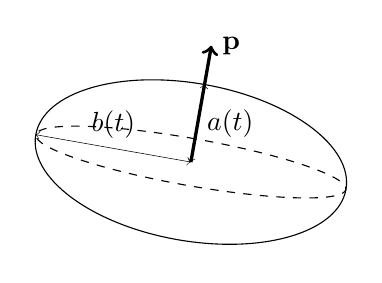
\begin{tikzpicture}[rotate=80]
        \draw(0,0) ellipse (1 cm and 2 cm);
        \draw[dashed](0,0) ellipse (0.3 cm and 2 cm);
        \draw[<->,very thin](0,0) --++ (1,0)node[midway,right]{$a(t)$};
        \draw[->,very thick](0,0) --++ (1.5,0)node[right]{$\textbf{p}$};
        \draw[<->,very thin](0,0) --++ (0,2)node[midway,above]{$b(t)$};
    \end{tikzpicture}
    \hfill
    \caption{Scheme of an  oblate spheroid oriented along the unit vector \textbf{p}.}
    \label{fig:scheme2}
\end{figure}
This tensor is defined such that its eigenvalues are the dimensionless square length of the semi-axis of the spheroid, such that $\textbf{C}_\alpha = a^2/r_0^2 \textbf{pp} + b^2 /r_0^2 (\textbf{I}-\textbf{pp})$ where $r$ is the radius of the sphere of same volume. 
This definition is convenient since it can be shown that $\textbf{C}_\alpha$ is equivalent to the Cauchy strain tensor well-defined in solid mechanics \citet{mwasame2017macroscopic}. 
Therefore, in a general coordinate system the point on the surface of the spheroid respect the equation, 
\begin{equation*}
    \textbf{r}\cdot\textbf{C}^{-1}\cdot\textbf{r} = r_0^2,
\end{equation*}
where $\textbf{C}$ is the inverse operator. 

Additionally, one can verify that the second order moment of mass of the particles is related to the conformation tensor through, $\textbf{M}_\alpha = \frac{m_\alpha  r_0^2}{5} \textbf{C}$. 
One can show that the constant volume constrain can be obtained by ensuring that $\text{det}(\textbf{C}) = (ab^2)^2 /(r_0^6) = 1$. 
It must be understood that at equilibrium the particle reach a spherical shape and therefore has $\textsc{C} = \textbf{I}$. 

\subsubsection*{The drop internal kinematic equation}



The evolution of $\textbf{C}_\alpha$ and $\bm\Gamma_\alpha$ will be described by the second moment of mass and first moment of momentum equation.
Consequently, we must reformulate the terms in \ref{eq:dt_M_alpha} and \ref{eq:dt_P_alpha} in terms of $\textbf{C}_\alpha$ and $\bm\Gamma_\alpha$. 
The integrals constitutive of these moments equations can be written, 
\begin{align}
    \intO{(\textbf{rw}_2^0 )_{ij}+ (\textbf{w}_2^0 \textbf{r})_{ij}} 
    = \textbf{C}_{\alpha,ik} \cdot \bm\Gamma_{\alpha,kj}
    +  \bm\Gamma_{\alpha,ki} \cdot \textbf{C}_{\alpha,jk}
    % +  \bm\Gamma_{\alpha,ij} + \bm\Gamma_{\alpha,ij}
    \\
    \intO{\rho_2 \textbf{w}_{2,i}^0\textbf{w}_{2,j}^0}
    = \frac{m_\alpha a^2}{5}
        \bm\Gamma_{\alpha,lj}\bm\Gamma_{\alpha,ki} \textbf{C}_{\alpha,kl} 
        % + \bm\Gamma_{\alpha,kj}\bm\Gamma_{\alpha,ki} 
        % + f_\textbf{ww}(\textbf{u}_\alpha,\textbf{C}_\alpha,\bm\Gamma_\alpha,\textbf{u}_1,\bm \Gamma_1,\phi_2)
        + \intO{\rho_2\textbf{w}^s_2\textbf{w}^s_2}
    \\
    \label{eq:sigma_2_def}
    \intO{\bm\sigma_{2,ij}^0}
    =
    % -\intO{p_2^0} \textbf{I}_{ij}
    \mu_2 v_\alpha (\bm\Gamma_{\alpha,ij} + \bm\Gamma_{\alpha,ij})
    + \mu_2 \intS{\textbf{w}^s_{2,i}\textbf{n}_{2,j}+ \textbf{w}^s_{2,j}\textbf{n}_{2,i}}
    + \textbf{I}_{ij}\intO{p_2^0} 
    \\
    \label{eq:sigma_I_def}
    \intS{\bm\sigma_{I,ij}^0}
    = \frac{2 \gamma v_\alpha }{a} \textbf{I}_{ij} - \frac{4 \gamma v_\alpha }{5 a} \textbf{C}_{\alpha,ij}
    +\mathcal(|\textbf{C}|^2)\\
    \intS{\textbf{r}\bm\sigma_1^0\cdot \textbf{n}_2}
    = 
    \frac{1}{2}\intS{(\textbf{r}\bm\sigma_1^0-\bm\sigma_1^0\textbf{r})\cdot \textbf{n}_2}
    + \frac{1}{2}\intS{(\textbf{r}\bm\sigma_1^0+\bm\sigma_1^0\textbf{r})\cdot \textbf{n}_2}
    % \textbf{M}(\textbf{u}_\alpha,\textbf{C}_\alpha,\bm\Gamma_\alpha,\textbf{u}_1,\bm \Gamma_1,\phi_2)
\end{align}
First, as discussed above only the deforming motion contribute to the symmetric part of the moment of momentum, we could therefore express it explicitly in terms of the particle unknown. 
Regarding the first moment of the surface tension, it has been computed analytically carrying a surface integral on the ellipsoidal surface of the droplet. 
Since, the droplets remain spheroidal under small deformation we choose to approximate $\intS{\bm\sigma_I^0}$ with its first order Taylor series in $\textbf{C}_\alpha$ without lost of generality.
Note that our expression of $\intS{\bm\sigma_I^0}$ is in agreement with \citet{lhuillier1987phenomenology} if one account for the slight difference of his definition of the deformation tensor which is half of $\textbf{C}_{\alpha}$. 
% in which our $\textbf{C}_\alpha$ is twice his, in the limit of small \textbf{C}_\alpha.
For the expression of $\intO{\rho_2 \textbf{w}_{2,i}^0\textbf{w}_{2,j}^0}$, $ \intO{\bm\sigma_{2,ij}^0}$ we had to introduce two unknown functions, $f_\textbf{ww}$, $f_{\bm{\sigma}}$, which vanish when $\textbf{w}^s_2 =0$. 
Therefore, these expressions are a sum of a function involving $\bm\Gamma_\alpha$ and an unknown part which depend on the parameters of the problem and need to be closed. 
The expression of $\intO{\rho_2 \textbf{w}_{2,i}^0\textbf{w}_{2,j}^0}$, $ \intO{\bm\sigma_{2,ij}^0}$ and $\intS{\textbf{r}\bm\sigma_1^0\cdot \textbf{n}_2}$ are very problem dependent. 
To provide a clearer example we computed these terms in \ref{ap:Translating_sphere} in the simplified scenario of an isolated droplet in a general linear flow. 
\begin{multline}    
    \frac{m_\alpha a^2}{10}\ddt^2 \textbf{C}_\alpha
    - \frac{m_\alpha a^2}{5}
    \bm\Gamma_{\alpha,lj}\bm\Gamma_{\alpha,ki} \textbf{C}_{\alpha,kl} 
    - \intO{\rho_2\textbf{w}^s_2\textbf{w}^s_2}\\
    + \mu_2 v_\alpha (\bm \Gamma_{p,ij}+\bm \Gamma_{p,ji})
    + \mu_2 \intS{\textbf{w}^s_{2,i}\textbf{n}_{2,j}+ \textbf{w}^s_{2,j}\textbf{n}_{2,i}}\\
    + \textbf{I}_{ij}\intO{p_2^0} 
    + \frac{2 \gamma v_\alpha }{a} \textbf{I}_{ij} 
    - \frac{4 \gamma v_\alpha }{5 a} (\textbf{C}_{ij} - \textbf{I}_{ij})
    =  
    + \frac{1}{2}\intS{(\textbf{r}\bm\sigma_2^0+ \bm\sigma_2^0\textbf{r})\cdot \textbf{n}}
\end{multline}
\begin{multline}    
    \frac{m_\alpha a^2}{10}\ddt^2 \textbf{C}_\alpha
    - \frac{m_\alpha a^2}{5}
    \bm\Gamma_{\alpha,lj}\bm\Gamma_{\alpha,ki} \textbf{C}_{\alpha,kl} 
    - \intO{\rho_2\textbf{w}^s_2\textbf{w}^s_2}\\
    + \mu_2 v_\alpha (
        \ddt \textbf{C}_{\alpha,ij}
         -(\textbf{C}_{\alpha,ik} - \textbf{I}_{ik}) \cdot \bm\Gamma_{\alpha,kj}
    -  \bm\Gamma_{\alpha,ki} \cdot (\textbf{C}_{\alpha,jk} - \textbf{I}_{\alpha,jk})
    )
    + \mu_2 \intS{\textbf{w}^s_{2,i}\textbf{n}_{2,j}+ \textbf{w}^s_{2,j}\textbf{n}_{2,i}}\\
    + \textbf{I}_{ij}\intO{p_2^0} 
    + \frac{2 \gamma v_\alpha }{a} \textbf{I}_{ij} 
    - \frac{4 \gamma v_\alpha }{5 a} (\textbf{C}_{ij} - \textbf{I}_{ij})
    =  
    + \frac{1}{2}\intS{(\textbf{r}\bm\sigma_2^0+ \bm\sigma_2^0\textbf{r})\cdot \textbf{n}}
\end{multline}
In the quasi steady regime all the derivative cancel out and $\bm\Gamma$ also,
\begin{multline}    
    % \frac{m_\alpha a^2}{10}\ddt^2 \textbf{C}_\alpha
    % - \frac{m_\alpha a^2}{5}
    % \bm\Gamma_{\alpha,lj}\bm\Gamma_{\alpha,ki} \textbf{C}_{\alpha,kl} 
    - \intO{\rho_2\textbf{w}^s_2\textbf{w}^s_2}
    + \mu_2 \intS{\textbf{w}^s_{2,i}\textbf{n}_{2,j}+ \textbf{w}^s_{2,j}\textbf{n}_{2,i}}\\
    + \textbf{I}_{ij}\intO{p_2^0} 
    + \frac{2 \gamma v_\alpha }{a} \textbf{I}_{ij} 
    - \frac{4 \gamma v_\alpha }{5 a} (\textbf{C}_{ij} - \textbf{I}_{ij})
    =  
    + \frac{1}{2}\intS{(\textbf{r}\bm\sigma_2^0+ \bm\sigma_2^0\textbf{r})\cdot \textbf{n}}
\end{multline}
Thus the stresslet might be computed upon known these integral but at this stage we could say ok just compute the stress let then. 
For bubbly flow we have the relation,
\begin{equation*}
+ \textbf{I}_{ij}\intO{p_2^0} 
+ \frac{2 \gamma v_\alpha }{a} \textbf{I}_{ij} 
- \frac{4 \gamma v_\alpha }{5 a} (\textbf{C}_{ij} - \textbf{I}_{ij})
=  
+ \frac{1}{2}\intS{(\textbf{r}\bm\sigma_2^0+ \bm\sigma_2^0\textbf{r})\cdot \textbf{n}}
\end{equation*}
In which case \textbf{C} is related to the pressure jump plus the stresslet while $\bm\Gamma$ isn't necessarily negligible. 

In this casethe stresslet appear to be, 
\begin{equation*}
    + \textbf{I}_{ij}\intO{p_2^0} 
    + \frac{2 \gamma v_\alpha }{a} \textbf{I}_{ij} 
    - \frac{4 \gamma v_\alpha }{5 a} (\textbf{C}_{ij} - \textbf{I}_{ij})
    - \mu_1 \intS{\textbf{w}^s_{2,i}\textbf{n}_{2,j}+ \textbf{w}^s_{2,j}\textbf{n}_{2,i}}
    - \mu_1 v_\alpha (\bm \Gamma_{p,ij}+\bm \Gamma_{p,ji})
    =  
    \intS{\textbf{r}\bm\sigma_2^0\cdot \textbf{n}}
    - \mu_1 \intO{e_2^0}
\end{equation*}
Then if we arrive to prove that $(\textbf{C}_{ij} - \textbf{I}_{ij}):\textbf{I}_{ij} = 0$ we recover a Laplace pressure like making $+ \textbf{I}_{ij}\intO{p_2^0} 
+ \frac{2 \gamma v_\alpha }{a} \textbf{I}_{ij} $ equal to the fluid pressure. 

At this point it wouldn't be wise trying to find an expression for each of these unknown functions in such a generality. 
Instead, we expose the unclosed set of equation of motions for spheroidal particles. 
In addition to the previously exposed equations (mass, momentum and energy equation) this system is constituted of three equations, one for $\textbf{C}_\alpha$ and two equation for the moment of momentum, the symmetric and skew-symmetric moment of momentum. 
% These read, 
% \begin{align*}
%     \ddt \textbf{C}_{\alpha,ij}
%     = \textbf{C}_{\alpha,ik} \cdot \bm\Gamma_{\alpha,kj}
%     +  \bm\Gamma_{\alpha,ki} \cdot \textbf{C}_{\alpha,jk},\\
%     \frac{a^2  m_\alpha}{5} \ddt( \textbf{C}_{ik} \cdot \bm\Gamma_{\alpha,kj}
%     -  \bm\Gamma_{\alpha,ki} \cdot \textbf{C}_{jk})
%     =  \intS{(\textbf{r}\bm\sigma_2^0- \bm\sigma_2^0\textbf{r})\cdot \textbf{n}}\\
%     \frac{m_\alpha a^2}{5}\ddt^2 \textbf{C}_\alpha
%     - \frac{m_\alpha a^2}{5}[
%     \bm\Gamma_{\alpha,lj}\bm\Gamma_{\alpha,ki} \textbf{C}_{\alpha,kl} + f_\textbf{ww}]
%     + \mu_2 v_\alpha [(\bm \Gamma_{p,ij}+\bm \Gamma_{p,ji})
%     + f_{\bm{\sigma}}]\\
%     + \frac{2 \gamma v_\alpha }{a} \textbf{I}_{ij} 
%     - \frac{4 \gamma v_\alpha }{5 a} (\textbf{C}_{ij} - \textbf{I}_{ij})
%     = \intS{(\textbf{r}\bm\sigma_2^0+ \bm\sigma_2^0\textbf{r})\cdot \textbf{n}}
%     % + \textbf{I}_{ij}\intO{p_2^0}
% \end{align*}
% Where we placed the unknown function at the right hands side of these equations. 
Now, we would like to propose a more intuitive interpretation of the mass and momentum equations.
To that end, we make the problem dimensionless by introducing, 
the \textit{Capillary number} $Ca= \frac{\mu_1 U}{\gamma}$, The viscosity ratio $\lambda = \mu_2/\mu_1$, the density ratio $\zeta = \rho_2/\rho_1$ and the Reynolds number $Re = \frac{a U \rho_1}{\mu_1}$, with $U$ as the velocity scale. 
%  such that  $\bm\Gamma_\alpha'  = \frac{a}{U}\bm\Gamma$, and $\tau_a$ the timescale related to the drop shape evolution.
In the low Reynolds regime the first moment of surface traction forces will be proportional to a viscous stress (see \ref{ap:Translating_sphere}), therefore :$\intS{\textbf{r}\bm\sigma_2^0\cdot \textbf{n}} =\mu_1  \tau v_\alpha \intS{\textbf{r}\bm\sigma_2^0\cdot \textbf{n}}^*$, with $\tau$ the inverse timescale of the external solicitation.
The ratio between the external flow scale $\tau$ and the drop timescale $\tau_a$ is noted $\beta$. 
With that in mind, \ref{eq:dt_M_alpha}, \ref{eq:dt_mu_alpha} and \ref{eq:dt_S_alpha} might be written :
\begin{align}
    \label{eq:dt_Cs}
    \beta \ddt \textbf{C}_{\alpha,ij}
    - \textbf{C}_{\alpha,ik} \cdot \bm\Gamma_{\alpha,kj}^*
    - \bm\Gamma_{\alpha,ki}^* \cdot \textbf{C}_{\alpha,jk},
    = 
    \bm\Gamma_{\alpha,ij}^*
    +  \bm\Gamma_{\alpha,ji}^*\\
    Re \zeta \beta \ddt( \textbf{C}_{\alpha,ik} \cdot \bm\Gamma_{\alpha,kj}^*
    -  \bm\Gamma_{\alpha,ki}^* \cdot \textbf{C}_{\alpha,jk}
    + \bm\Gamma_{\alpha,ji} - \bm\Gamma_{\alpha,ij})
    =  \intS{(\textbf{r}\bm\sigma_2^0- \bm\sigma_2^0\textbf{r})\cdot \textbf{n}}^*\\
    \zeta Re \frac{1}{5}  
    \left[
        \frac{1}{2}\beta^2 \ddt^2_* \textbf{C}_\alpha
        - \bm\Gamma_{\alpha,lj}^* \bm\Gamma_{\alpha,ki}^* \textbf{C}_{\alpha,kl}^* 
        - \bm\Gamma_{\alpha,kj}^* \bm\Gamma_{\alpha,ki}^* 
        - f_\textbf{ww}
    \right]\nonumber\\
    + \lambda \left[
        \beta \ddt \textbf{C}_{\alpha,ij}
        -\textbf{C}_{\alpha,ik} \cdot \bm\Gamma_{\alpha,kj}
        - \bm\Gamma_{\alpha,ki}^* \cdot \textbf{C}_{\alpha,jk},
        + f_{\bm{\sigma}}
    \right]\nonumber\\
    - \frac{1}{Ca}\left[
        \frac{4}{5} \textbf{C}_{\alpha,ij}
        +2 \textbf{I}_{ij} 
    \right]
    =
    \frac{1}{2}\intS{(\textbf{r}\bm\sigma_1^0+ \bm\sigma_1^0\textbf{r})\cdot \textbf{n}}^*
    \label{eq:dt2_C}
\end{align}







The drop internal velocity will be assumed to be linear and homogeneous such as if it was a solid deformable displacement. 
It must be said that due to the presence of surface tension and relative velocity this hypothesis isn't physical. 
Indeed, on one hand inhomogeneous stresses such as surface tension stress, might induce inhomogeneous internal flow \citep{goddard1967nonlinear}, and obviously the relative motion will evidently induce a Hill's vortex-like internal motions. 
Therefore, in a second step the modeling of internal flow will include quadratic terms but for ow we restrict our attention to linear internal flow fields. 
Taking into account this assumption the drop internal velocity field can be written,
\begin{equation}
    \textbf{w}_2^0(\textbf{x}_\alpha)
    = \bm\Gamma_\alpha \cdot \textbf{r}
    =\bm{\Omega}_\alpha\cdot \textbf{r}
    + \textbf{E}_\alpha \cdot \textbf{r}
    \label{eq:def_vel}
\end{equation}
where $\bm\Gamma_\alpha$, is the velocity gradient for any point inside the domain $\Omega_\alpha(t)$, and $\textbf{E}_\alpha$ represents the rate of strain or the symmetric part second order tensor, and $\bm\Omega_\alpha$ the angular velocity pseudo vector. 

The evolution of the internal kinematic of the droplet, i.e. the shape, will be described by the second moment of mass equation, to which we substitute the tensor $\mathcal{M}_\alpha$ by \textbf{C} to obtain an equation for the deformation. 
It yields, 
\begin{equation*}
    \ddt \textbf{C}_{ij}
    = \textbf{C}_{ik} \cdot \bm\Gamma_{\alpha,kj}
    +  \bm\Gamma_{\alpha,ki} \cdot \textbf{C}_{jk}.
    \label{eq:dt_C}
\end{equation*}
From this point one can relate $\bm\Gamma_{\alpha,kj}$ to the fluid mean kinematic properties. 
In pure shear flow for example, if one consider the problem of a slightly deformable droplet one can show that, $\bm\Gamma \sim \Gamma_1(\textbf{x}_\alpha)$ where $\bm\Gamma_1$ is the local fluid velocity gradient.
From this consideration one can find back the classical models such as the one of  \citet{maffettone1998equation,schowalter1968rheological}. 

In our current problem, rising inertial droplets, we must thus seek for an expression linking the drop internal velocity gradient $\bm\Gamma_\alpha$ with the relative motion $\textbf{u}_{pf}$. 
This is done through the consideration of the second moment of momentum equation. 

\subsubsection*{The dynamical droplet equations}

Objective : 
\begin{equation*}
    \bm\sigma 
    = 
    - \phi_1 p_1 \textbf{I}
    - \mu_1 \textbf{e}
    + \phi_2(\bm\sigma_2 - \bm\sigma_1)
    + \phi_I\bm\sigma_I
\end{equation*}

The dynamic of the droplet will be described by the use of the symmetric moment of momentum equation presented in \ref{sec:Lagrangian}.
We will therefore need constitutive equation for the particle internal and surface stress. 
The particle internal stress is described by a Newtonian behavior law yielding directly, 
\tb{hypothèse}
\begin{equation*}
    \intO{\bm\sigma_2^0}
    = - \intO{p_2^0} \delta_{ij}
    + v_\alpha \mu_2 \textbf{E}_{\alpha,ij}.
\end{equation*} 
Equally, if the particle were constituted of any other material one could include the adapted constitutive law in this term. 
Regarding the particle surface stress, it can be computed analytically since we assumed a spheroidal shape. 
% Indeed, all the points on the surface of the particle can describe by the equation, $\textbf{r}\cdot\textbf{C}^{-1}-1=0$ which mean that the normal vector at the surface can be express as $\textbf{n}_2 = 2\textbf{H}\cdot\textbf{r}$ and it follow the tensorial expression of the local stress. 
The details are not given here but the results at $\mathcal{O}(|\textbf{C}|^3)$  and $\mathcal{O}(|\textbf{C}|^2)$ accurate yield, 
\begin{align*}
    \pSavg{\bm\sigma_I^0}
    &= \frac{\gamma v 2}{r} \left[
        1  + \frac{1}{20 } (\textbf{C}_{-\textbf{I}}:\textbf{pp})^2 
        + \frac{4}{20 } [\textbf{C}_{-\textbf{I}}:(\textbf{I}-\textbf{pp})]^2\right] \textbf{I}\\
        &- \frac{\gamma v}{35 r} \left[ 28 \textbf{C}_{-\textbf{I}}
        + 4[\textbf{C}_{-\textbf{I}}\cdot \textbf{C}_{-\textbf{I}} + 15 (\textbf{C}_{-\textbf{I}}:\textbf{pp})^2\textbf{pp}]
        \right]
        +\mathcal{O}(|\textbf{C}|^3)\\
    &= \frac{\gamma v 2}{r} \textbf{I} - \frac{\gamma v 4}{5 r} (\textbf{C} - \textbf{I})
    +\mathcal(|\textbf{C}|^2)
\end{align*}
Note that the first term of the first equality correspond to $\frac{2\gamma}{3}s_\alpha$, it is therefore $\frac{2}{3}$ of the surface energy which varies only at $\mathcal{O}(|\textbf{C}|^2)$. 
The second term account for the deviatoric part of the stress tensor which is of $\mathcal{O}(\textbf{C})$. 
The results at first order are agreements with \citet{lhuillier1987phenomenology} when accounting for the different definition of the conformation tensor \textbf{C} that he used.

The moment of momentum equation with an internal velocity such as it is described by \ref{eq:def_vel} is then given by the expression,
\begin{multline}
    \ddt (\textbf{C}_{\alpha,ik} \bm\Gamma_{\alpha,kj})
    -\bm\Gamma_{\alpha,lj}\bm\Gamma_{\alpha,ki} \textbf{C}_{\alpha,kl}
    = 
    % \intO{p_2^0} \delta_{ij}
    - \frac{5\mu_2}{a^2\rho_2}  \textbf{E}_{\alpha,ij}
    + \frac{\gamma 6 }{\rho_2 a^3} \textbf{I} 
    - \frac{\gamma 4}{\rho_2 a^3} \textbf{C}_{\alpha,ij} 
    +\frac{5}{a^2 \rho_2 v_\alpha} \pavg{\textbf{r}\bm\sigma_1^0\cdot\textbf{n}_2}_{ij},
    \label{eq:moment_of_momentum}
\end{multline}
Or its symmetric part,
\begin{multline}
    \ddt^2 (\textbf{C}_{\alpha,ik})
    - 2\bm\Gamma_{\alpha,lj}\bm\Gamma_{\alpha,ki} \textbf{C}_{\alpha,kl}
    = 
    % \intO{p_2^0} \delta_{ij}
    - 2\frac{5\mu_2}{a^2\rho_2}  \textbf{E}_{\alpha,ij}
    + 2\frac{\gamma 6 }{\rho_2 a^3} \textbf{I} 
    - 2\frac{\gamma 4}{\rho_2 a^3} \textbf{C}_{\alpha,ij} 
    + 2\frac{5}{a^2 \rho_2 v_\alpha} \pavg{\textbf{r}\bm\sigma_1^0\cdot\textbf{n}_2}_{ij},
    \label{eq:moment_of_momentum}
\end{multline}
\tb{The internal velocity is way more to complicated one must use Hill vortex}
\tb{The isotropic part might cancel the difference in pressure.}
where the only undetermined term is the first moment of the hydrodynamic forces. 
While deriving \ref{eq:moment_of_momentum} we made absolutely no hypothesis on the dilute nature of the flow nor on its potentially inertial effect.
Therefore, solely the first moment of hydrodynamic force might be able to take in account the effect of finite volume fraction, inertial effect, particle interaction\ldots
Therefore we introduce the function,
\begin{align*}
    \pavg{\textbf{r}\bm\sigma_1^0\cdot\textbf{n}_2}_{ij}
    = \textbf{f}_{1,ij}(\textbf{u}_\alpha - \textbf{u}_1,\bm\Gamma_\alpha - \bm\Gamma_1, \textbf{C}_{\alpha},Re,\phi) 
\end{align*}
which depends on the particles fluid relative properties, $(\textbf{u}_\alpha - \textbf{u}_1,\bm\Gamma_\alpha - \bm\Gamma_1)$ and problem dimensionless number $Re,\phi$. 
Such a relation have been found in \citet{goddard1967nonlinear}. 

In \citet{raja2010inertial} they consider a deformable drop in shearing inertial flow. 
Their expression (3.18) for the particle contribution to the suspension stress is in fact a combination of \ref{eq:moment_of_momentum} and \ref{eq:dt_C} where the first moment $\pavg{\textbf{r}\bm\sigma_1^0\cdot\textbf{n}_2}_{ij}$ have been solved analytically in terms of $\bm\Gamma_1$.

Therefore, in the continuity of their work we now wish to determine $\pavg{\textbf{r}\bm\sigma_1^0\cdot\textbf{n}_2}_{ij}$ in a pure translating motion with no mean shear. 
It is known from the singularity solution of stokes flow that $\pavg{\textbf{r}\bm\sigma_1^0\cdot\textbf{n}_2}_{ij} = 0$ for a non-inertial spherical droplet in pure translation. 
However, when finite inertia effects appear the first moments of surface traction is not null and the drop deform into a spheroid proportionally the relative velocity $\textbf{u}_{fp}$. 


\subsubsection*{Determination of the shape based on \citet{taylor1964deformation} theoretical results}

In the last section we assumed an arbitrary spheroidal drop within a suspension. 
Now we consider that the drop is only subject to a relative motion with the fluid. 
Our goal is still to express the stress within the suspension. 

In \citet{taylor1964deformation} they derive the shape and the drag force of a translating droplet at $\textbf{O}(Re^2)$ in a steady state situation. 
Although they did not directly derive the stress let they provide a formula for the shape as a function of the relative velocity. 
In \citet{taylor1964deformation} they give an explicit formula for the deformation in terms of the Reynolds number $Re$ based on the relative velocity fields, $\textbf{u}_\alpha - \textbf{u}_1$. 
The dimensionless radius of the droplets can be express in the polar coordinate reference frame of the drop as, 
\begin{equation*}
    \frac{R_\text{taylor}(\theta)}{a} = 1 - \beta \textit{We} P_2(\cos\theta)
    + \mathcal{O}(Re^3)
\end{equation*}
where $Re = |\textbf{u}_{pf}| a /\nu_1$, $P_2(\cos\theta)$ is the Legendre polynomial of degree two and $\kappa$ is a coefficient related to physical parameters given in \citet{taylor1964deformation}.  
This solution need to satisfy $\kappa Re \ll 1$ and $Re \ll 1$ to be valid. 
These, 
% \begin{center}
%     \begin{tikzpicture}[gradient arrow/.style={
%         insert path={coordinate[pos=#1,sloped,
%             above=\pgfkeysvalueof{/tikz/ga/above}]  (aux-1)
%            coordinate[pos=#1,sloped,
%             above=\pgfkeysvalueof{/tikz/ga/above}+\pgfkeysvalueof{/tikz/ga/length}] (aux-2)
%            (aux-1) edge[/tikz/ga/arrow] 
%            (aux-2)}},ga/.cd,
%            above/.initial=3pt,
%            length/.initial=12pt,
%            arrow/.style={-stealth,black,solid,thick}]
%          \begin{axis}[scale=0.85,xmin=-4,xmax=12, ymin=-4,ymax=4,x=1cm,y=1cm,at={(-4cm,-4cm)}]
%           \addplot +[no markers,name=contour,
%            raw gnuplot,
%            thick,dashed,
%            empty line = jump, % not strictly necessary, as this is the default behaviour in the development version of PGFPlots
%            ] gnuplot {
%                set contour base;
%                set cntrparam levels discrete -2,-1.1,-1.4;
%                unset surface;
%                set view map;
%                set isosamples 500;
%                set samples 500;
%                splot -2/sqrt((x-7.5)^2+y^2)-3/sqrt((x-0.5)^2+y^2);
%            } 
%         %    [pos segment=1]
%         %    [gradient arrow/.list={0.2,0.8}]
%         %    [pos segment=3,/tikz/ga/arrow/.append style={red},/tikz/ga/length=10pt]
%         %    [gradient arrow/.list={0.2,0.8}];
%          \end{axis}
%     \end{tikzpicture}
% \end{center}
Upon assuming a quasi steady state regime which correspond to a droplet response time $\frac{1}{\tau_a^2} \ll \frac{\mu_1 U \lambda }{a^3\rho_2} \approx \frac{\mu_1 U \lambda }{a^3\rho_2 Ca} \approx \frac{\mu_1 U \lambda }{a^3\rho_2}$ we can stipulate that the shape of the droplet is instantaneously correlated with the velocity. 
In this hypothesis it is clear that the shape of the droplet is correlated at any time with the local motion of the flow $\textbf{u}_{fp}$. 
The conformation tensor principal values, are related to \citet{taylor1964deformation} formula through,
\begin{align*}
    \textbf{C}(\textit{We})
    % = \left(\frac{R_\text{taylor}(0)}{a}\right)^2
    = (1 - \beta \textit{We} )^2 \textbf{pp}
    + 
     (1 + \beta \textit{We}/2  )^2 (\textbf{I}-\textbf{pp})
\end{align*}
where $\textit{We}$ is the \textit{Weber} number defined as $\textit{We} = \rho_1 a \textbf{u}_{\alpha f}\cdot\textbf{u}_{\alpha f}/\sigma$. 

Now that we obtained the shape as a function of the relative velocity, we aim to recover the rate of deformation of the drop through the second moment of mass equation. 
The droplet interior flow is a complex function of space and time. 
We assumed small deformation such that our spherical particle become a spheroid. 
Therefore, the velocity fields responsible for the shape change is a linear function of the position, thus $\textbf{w}_2^0 = f(\textbf{r}) + \bm\Gamma_\alpha(t,\FF) \cdot \textbf{r}$, where $f(\textbf{r})$ is the steady state internal motion and $\bm\Gamma_\alpha(t,\FF)$ is a time dependent matrix describing the homogeneous deformation of the droplets. 
The complex recirculation structure such as Hill vortexes-like doesn't contribute to the symmetric part of the moment of momentum as it is not changing the shape of the particle. 
The only contribution to the stretching of momentum is therefor the second term. 
Additionally, we always consider the drop deformation in the direction of the flow. 
Now that the drop shape is fully determined by the local Reynolds number the second order of mass equation can be use to determine the inner rate of strain of the drop,
\begin{equation*}
    \ddt \textbf{C}_{ij}
    = \textbf{C}_{ik} \cdot \bm\Gamma_{\alpha,kj}
    +  \bm\Gamma_{\alpha,ki} \cdot \textbf{C}_{jk}.
\end{equation*}
This equation must be solved for the $\Gamma_{ki}$ as $\textbf{C}$ is a known function of $\textbf{u}_{pf}$ and the physical parameters. 

As mentioned above the surface tension stress can be estimated to be an instantaneous function of \textbf{C}, namely, 
\begin{align*}
    \pSavg{\bm\sigma_I^0}
    = \frac{\gamma v 2}{r} \textbf{I} - \frac{\gamma v 4}{5 r} (\textbf{C} - \textbf{I})
    +\mathcal(|\textbf{C}|^2)
\end{align*}
At this stage the only remaining term to determine the contribution to the suspension stress is an expression of the particle stress tensor as a function of \textbf{C} ad $\bm\Gamma$. 
The symmetric part of the moment of momentum equation can be written,
\begin{equation*}
    \ddt^2\intO{\textbf{C}_{ij}}
    -\intO{\rho_2\textbf{w}_{2,i}^0\textbf{w}_{2,j}^0}
    + \intO{\bm\sigma_{2,ij}^0}
    + \intS{\bm\sigma_{I,ij}^0}
    = \intS{(\textbf{r}\bm\sigma_1^0+ \bm\sigma_1^0 \textbf{r})_{ijk}\cdot \textbf{n}_{2,k}}
\end{equation*}
At this stage we must either find the complete closure for $\textbf{w}_{2,i}^0$ which will enable us to find an expression for one of the two remaining terms.
And by solving this equation one might obtain the last one terms in terms of $\bm\Gamma$ and \textbf{C}. 
\tb{Either find the singularity sol or assume linear displacement}

We're assuming that the rate of strain is the only contribution to the stress, which might be justified by the fact that Hill's vortexes resultant vanish for spherical drops. 
Thus, the drop interior stress might be written, 
\begin{equation*}
    \pSavg{\bm\sigma_2^0}
    =-\pOavg{p_2^0} 
    + \mu_2 n_p (\bm\Gamma_{p,ij}+\bm\Gamma_{p,ji})
\end{equation*}
Then the set of equation needed to describe the rheology of a dilute suspension of inertial drops is, 
\begin{align*}
    \textbf{C}_p(\textit{We})
    % = \left(\frac{R_\text{taylor}(0)}{a}\right)^2
    = (1 - \beta \textit{We} )^2 \textbf{pp}
    + 
     (1 + \beta \textit{We}/2  )^2 (\textbf{I}-\textbf{pp})\\
    \pavg{\ddt \textbf{C}_{ij}}
    = \textbf{C}_{p,ik} \cdot \bm\Gamma_{p,kj}
    +  \bm\Gamma_{p,ki} \cdot \textbf{C}_{p,jk}.\\
    \bm\sigma^\text{dev}
    = 
    \mu_1 \textbf{e}_{ij}
    +  n_p (\mu_2 - \mu_1) (\bm\Gamma_{p,ij} + \bm\Gamma_{p,ji})
    + n_p \frac{\gamma  4}{5 r} (\textbf{C}_{p,ij} - \textbf{I}_{ij})
\end{align*}

Under this assumption it is observed that $\textbf{C}\sim U^2$ has the same form as the pseudo turbulence Reynolds stress computed in potential flow. 
Indeed, 
The deviatoric part of the conformation tensor can be written exactly as, 
\begin{equation*}
    \textbf{C} - \textbf{I}  = - 3 \beta \textit{We} \textbf{pp} +  \beta \textit{We} \textbf{I}
    + (\beta^2 \textit{We}^2 3/4) \textbf{pp} + \beta^2 \textit{We}^2/4 \textbf{I} 
\end{equation*}
We now stipulate that the deformation occur in the direction of the velocity difference such that the relative phase velocity of the particle $\alpha$ is written, $\textbf{u}_{\alpha f} = |\textbf{u}_{\alpha f}|\textbf{p}$, in this case the conformation tensor can be expressed, 
\begin{equation}
    \textbf{C}(\textbf{u}_{\alpha f}) - \textbf{I}  =  \frac{ \rho_1 a \beta}{\gamma} \left[
        -  3
        \textbf{u}_{\alpha f}\textbf{u}_{\alpha f}+   \textbf{u}_{\alpha f}\cdot\textbf{u}_{\alpha f}\textbf{I}
    \right]
    +\textbf{u}_{\alpha f}\cdot\textbf{u}_{\alpha f}\left(\frac{ \beta \rho_1 a}{\gamma}\right)^2
    \left[
        \frac{3}{4}
        \textbf{u}_{\alpha f}\textbf{u}_{\alpha f}
        +
        \frac{1}{4}
        \textbf{u}_{\alpha f}\cdot\textbf{u}_{\alpha f}
        \textbf{I}
    \right]
    \label{eq:C_def_with_u}
\end{equation}
This tensor is the particle confirmation tensor of the particle $\alpha$. 
We now apply an average procedure, and by that, $\pavg{\textbf{u}_{\alpha f}\textbf{u}_{\alpha f}} = \textbf{u}_{pf}\textbf{u}_{pf} + \pavg{\textbf{u}_\alpha'\textbf{u}_\alpha'}$ to gather with the assumption that the higher order fluctuation terms becomes negligible we obtain, 
\begin{multline*}
    \textbf{C}_p - \textbf{I}  =  \frac{ \rho_1 a \beta}{\gamma} \left[
        -  3
        \textbf{u}_{\alpha f}\textbf{u}_{\alpha f}
        +   (\textbf{u}_{\alpha f}\cdot\textbf{u}_{\alpha f})\textbf{I}
    \right]\\
    +\textbf{u}_{\alpha f}\cdot\textbf{u}_{\alpha f}\left(\frac{ \beta \rho_1 a}{\gamma}\right)^2
    \left[
        \frac{3}{4}
        \textbf{u}_{p f}\textbf{u}_{p f}
        +
        \frac{1}{4}
        (\textbf{u}_{p f}\cdot\textbf{u}_{p f})
        \textbf{I}
    \right]
    + \pavg{\textbf{C}(\textbf{u}_\alpha')}
\end{multline*}
where the last term correspond to \ref{eq:C_def_with_u} with $\textbf{u}_\alpha'$ is input velocity. 
Under these quite restrictive assumption we have shown that the surface tension contribution to the bulk stress have the same functional form as the Reynolds stress in potential flows \citet{van1982bubble}. 
\section*{fluid phase stress}
Already, we can see that the equivalent stress of the fluid phase is the made of the average fluid stress represented by the two first terms on the right hands side of \ref{eq:sigma_eq_0}. 
The first moment $\pSavg{\textbf{r}\bm{\sigma}_1^0 \cdot \textbf{n}_2}$ appearing in \ref{eq:sigma_eq_0} posses a skew-symmetric part and a symmetric part, the latter corresponding to the stresslet (see \ref{eq:stresslet_def}).
However, for non-solid particles \ref{eq:stresslet_def} is not entirely valid since in stokes theory the quantity referred as the stresslet is defined as \citet{pozrikidis1992boundary,kim2013microhydrodynamics},
\begin{equation}
    \label{eq:stresslet_def}
    n_p \mathscr{S}_{p,ki}
    = \frac{1}{2}
    \pSavg{
        r_k \sigma_{il}n_l + r_i \sigma_{kl}n_l 
        - \delta_{ik}
        \frac{2}{3}
        r_l \sigma_{lk}n_k
        - 2 \mu_f (u_k n_i+u_i n_i)
    }
\end{equation}
Likewise, we introduce the average skew symmetric part $\mathscr{L}_p$ and the average trace of the first moments $\mathscr{D}_p$ such as, 
\begin{align}
    \label{eq:torque_def}
    n_p \mathscr{L}_{p,ki}
    = \frac{1}{2}\pSavg{ r_k \sigma_{il}n_l - r_i \sigma_{kl}n_l }\\
    \label{eq:trace_def}
    n_p \mathscr{D}_{p,ij}
    = \frac{1}{3}\pSavg{ r_k (\sigma_{kl} + p_1 \delta_{kl})n_l } \delta_{ij}
    - n_p v_p p_1 \delta_{ij}
\end{align}
where we have retrieved the mean pressure from the trace of the first moments, so that we make appear the hydrostatic pressure  $n_p v_p p_1 \bm\delta$ explicitely.  
Notice that the volume fraction $\phi_1$ is present in front of the averaged pressure terms in \ref{eq:sigma_eq_0}.  
In various study \citep{prosperetti2009computational,chu2016flux}, this term is shown to be problematic  since it might generate nonphysical flux of momentum. 
However, as shown above and pointed out by  \citet{zhang1997momentum,jackson1997locally}, the first moment of hydrodynamic force tensor contains a part of the hydrostatic pressure.
With that contribution the total pressure in the fluid stress reach $\phi_1p_1 + n_p p_1 \approx p_1$ which is consistent.
Additionally, as seen in \ref{sec:two-fluid} the Reynolds stress is related to the pseudo turbulent kinetic energy through $\avg{\chi_1 \rho_1\textbf{u}_1'\textbf{u}_1'} : \bm\delta = 2k_1$ . 
Therefore, we can write, $\avg{\chi_1 \rho_1\textbf{u}_1'\textbf{u}_1'} = 2 \rho_1 k_1 \bm\delta + \avg{\textbf{u}_1'\textbf{u}_1'}^\text{dev}$ where the second term is the deviatoric part of the Reynolds stress. 

These remarks motivate us to rewrite the equivalent fluid phase stress under the general expression,  
\begin{multline*}
    \bm{\sigma}_1^\text{eq}
    = 
    \underbrace{p_1  \bm\delta
    - \mu_1 \textbf{e} }_\text{Newtonian fluid stress}
    +  \underbrace{\phi_1 k_1 \bm\delta
    + \rho_1 \avg{\chi_1\textbf{u}_1'\textbf{u}_1'}^\text{dev}}_\text{fluctuating stresses}
    - \underbrace{(n_p \mathscr{S}_p
    + n_p \mathscr{L}_p
    + n_p \mathscr{D}_p )}_\text{interfacial particles stresses}\\
    % + \mu_1  \pSavg{{\textbf{u}_1\textbf{n}_2 + \textbf{n}_2 \textbf{u}_1}}
    % - n_p \textbf{F}_\text{p}
    % + n_p \textbf{F}_\text{pfp} 
    + \frac{1}{2} \div \underbrace{\left[
        \pSavg{\textbf{rr}\bm{\sigma}_1^0\cdot \textbf{n}_2}
        + 2\pOavg{\mu_1 \textbf{re}_2^0 }
        + \ldots
        \right]
        }_\text{inhomogeneous particles stresses}
    \label{eq:sigma_eq1_def}
\end{multline*}
% with, 
% \begin{equation*}
%      \bm{\Sigma}
%     = 
%      \pMSavg{\textbf{rr} \bm{\sigma}_1^0\cdot \textbf{n}_2}
%      -\pMOavg{\mu_1 \textbf{r} \textbf{e}_2 }\\
% \end{equation*}
The contribution of the fluid phase equivalent pressure is made of,
the averaged $p_1$, the fluctuating part of the moment of force traction $\mathscr{D}_p$, and the fluid pseudo turbulent energy, $\phi_1 k_1$. 
The deviatoric part of the stress is constituted of the deviatoric part of the Reynolds stress $\avg{\chi_1\textbf{u}_1'\textbf{u}_1'}^\text{dev}$, the mean fluid shear rate $\mu_1 \textbf{e}$, the stresslet $\mathscr{S}_p$ and the hydrodynamic torque $\mathscr{L}_p$. 
The higher order moments found in $\bm{\Sigma}$ are not necessarily negligible, as shown in \citet{lhuillier1996contribution,jackson1997locally}, in fact they exhibit a different physical meaning. 
The first order moments will be function of the mean gradient of the fluid velocity while the other will be function of the background relative motion. 

\tb{a enlever}
It is known that the $n_p \mathscr{S}_p$ plays a significant role in the determination of the equivalent viscosity of the mixture. 
Therefore, it is of major importance to be able to measure it in DNS or experiment.
As, demonstrated by the expression of the ensemble averaged stress it is quite difficult to obtain such an information by experimental means, since it is mixed among other stresses.  
In DNS however we have access to pretty much any information, nevertheless surface integration of the stress can be shown to be inaccurate when performing volume of fluid method. 
Therefore, we propose the following formulas based on \ref{eq:dt_hybrid_Sp} which enable us to compute the stresslet by almost only volume integration,  


The last integral accounting for surface tension cannot be converted to volume integral. 
However, this integral is related only to the geometry of the interface. 
Besides, note that the pressure is absent as $\mathscr{S}_p$ is traceless. 

\begin{multline}    
    + n_p \mathscr{S}_p
    =
    \frac{1}{2}\pavg{\ddt^2{\textbf{M}_\alpha^\text{dev}}}
    - \pOavg{\left(
    \rho_2\textbf{w}_2^0 \textbf{w}_2^0
    - \rho_2\frac{1}{3}(\textbf{w}_2^0 \cdot \textbf{w}_2^0)\bm\delta\right)}\\
    + \mu_1 (\lambda - 1)\pOavg{\textbf{e}_2^0}
    + \pSavg{\gamma\left(\frac{1}{3}\bm\delta-\textbf{nn}\right)}\\
\end{multline}



\subsection{The bulk stress in dispersed multiphase flow}



Now that the architecture of the averaged dispersed multiphase flow equation is clarified, we would like to present the expression of the bulk stress tensor in a suspension of inertial particles subject to an arbitrary local body force field, $\textbf{b}^0$.
Firstly, is important to recall the definition of the \textit{bulk stress}. 
We define the \textit{bulk stress} tensor as a force applied on the fluid and on the particles phase, having the form $\div \bm{\Sigma}$, which added to the total external force $\textbf{B}$, balance exactly the material derivative of the mixture momentum : $\frac{D \rho \textbf{u}}{Dt}$. 
In this definition $\textbf{B}$ cannot be decomposed into a vector and a divergence of a tensor, in which case the latter would just contribute to $\bm{\Sigma}$.

We first expose the averaged mixture momentum and angular momentum equation easily derived from \ref{eq:dt_avg_f}, 
\begin{align}
    \pddt (\rho u_i)
    + \partial (\rho u_iu_k
    + \sigma_{ik}^\text{eq})
    = b_i\\
    \epsilon_{ijk} \sigma_{jk}
    = 0 
    \label{eq:momentum_bulk}
\end{align}
In the momentum equation we have defined, $\sigma_{ik}^\text{eq} = \avg{\rho\textbf{u}'\textbf{u}'}
- \avg{\chi_1\bm{\sigma}_1^0}-\avg{\chi_2\bm{\sigma}_2^0} - \avg{\delta_I \bm{\sigma}_I^0}$. 
Additionally, in the averaged angular momentum equation we have assumed that no-body torque exist at the local scale making the second equality equal to $0$ \citet{leal2007advanced} and the averaged mixture stress $\bm{\sigma}$ a symmetric quantity. 
However, note that $\bm{\sigma}$ is not exactly equal to the \textit{bulk stress} tensor $\bm{\Sigma}$ since $\textbf{b}$ can be expressed as a divergence of a stress.
Indeed, have defined $\textbf{b} = \textbf{B} + \div  \pMOavg{\textbf{b}_2^0}$ where $\textbf{B} = \phi_1 \textbf{b}_1 +  \pOavg{\textbf{b}_2^0 }$ and  $\pMOavg{\textbf{r}\textbf{b}_2^0}$ is defined accordingly to the previous definition. 
It follows the definition of the \textit{bulk stress} : 
\begin{equation}
    \bm{\Sigma}
    = 
    \avg{\rho\textbf{u}'\textbf{u}'}
    - \avg{\chi_1\bm{\sigma}_1^0}
    - \avg{\chi_2\bm{\sigma}_2^0} 
    - \avg{\delta_I \bm{\sigma}_I^0}
    - \pMOavg{\textbf{r}\textbf{b}_2^0}
\end{equation}
which proves already, in the absence of particles moments of the body forces $\pMOavg{\textbf{r}\textbf{b}_2^0}$, the antisymmetric part of the suspension stress is null, in agreement with \citet{dolata2020heterogeneous}.
% This skew symmetric part can be written in vector form as, 
% \begin{equation*}
%     \epsilon_{ijk}\textbf{T}_{jk}
%     = 
%     -\epsilon_{ijk} \pOavg{r_kb_j}
%     -\epsilon_{ijk}\frac{1}{2}\partial_l \pOavg{r_lr_kb_j}
%     = 0  
% \end{equation*}
We recall that the carrier fluid is a Newtonian fluid, therefore we may express the fluid phase stress as, 
\begin{equation}
    \phi_1 \sigma_{1,jk}
    = -p_1 \delta_{jk}
    + \mu_1 e_{jk}
    - \mu_1 \phi_2 e_{2,jk}. 
\end{equation} 
Additionally, we use the methodology of \citep{lhuillier1992volume,lhuillier1996contribution} to re express the averaged particle stress terms. 
The divergence of the particle phase stress may be expressed using \ref{eq:f_exp}, 
\begin{align}
    \label{eq:exp_sigma22}
    \partial_k \avg{\chi_2 {\sigma}_2^0}_{ik}
    &=  \partial_k\pOavg{ {\sigma}_{2,ik}^0}
    -\frac{1}{2} \partial_k\partial_j
    \pOavg{ r_j{\sigma}^0_{2,ik} + r_k\sigma^0_{2,ij}}
    + \ldots  \\
    \label{eq:exp_sigmaI2}
    \partial_k \avg{\delta_I {\sigma}^0_I}_{ik} 
    &=  \partial_k\pSavg{ {\sigma}_{I,ik}^0 }
        -\frac{1}{2} \partial_k\partial_j \pSavg{ r_j {\sigma}_{I,ik}^0+r_k {\sigma}_{I,ij}^0 }
        + \ldots  
\end{align}
Note that the heterogeneous terms must remain symmetric in the index $kj$ due to the double contraction with the operator $\partial_k\partial_j$, thus only the symmetric part in $jk$ remain and the terms such as, $\pOavg{ r_j{\sigma}^0_{2,ik} - r_k\sigma^0_{2,ij}}$ vanish. 
Upon the use of the moment of momentum equation of the first and second order we can easily derive these expressions, 
\begin{align}
    \intS{ (\bm{\sigma}_I)_{ik}}
    +\intO{ (\bm{\sigma}_2^0)_{ik}}
    = 
    \intO{ \rho_2 
    (\textbf{w}_2^0\textbf{w}_2^0  )_{ik}
    }
    -\ddt \intO{ r_i (\textbf{u}^0_2)_k }
    +\intS{ 
        b_{i}
        r_k 
    }
    +\intS{ 
     r_i (\bm{\sigma}_1^0 \cdot \textbf{n}_2)_{k}
    }
    \label{eq:dt_P_alpha}\\
    \intO{ r_{j}(\bm{\sigma}^0_2)_{ik}+r_{k}(\bm{\sigma}^0_2)_{ji}}
    +\intS{ r_{j}(\bm{\sigma}^0_I)_{ik}+r_{k}(\bm{\sigma}_I^0)_{ji}}
    = 
    - \ddt\intO{ \rho_2 (\textbf{u}_2^0)_i r_j r_k }\nonumber\\
    + \intO{ \rho_2 (r_{j} (\textbf{w}_2^0)_k (\textbf{u}^0_2)_i + r_k (\textbf{w}_2^0)_j (\textbf{u}^0_2)_i)}
    +\intS{  r_{k}r_{j} (\bm{\sigma}_1^0)_{il} (\textbf{n}_2)_l }
    + \intO{ r_{k}r_{j}  \rho_2 b_i } 
    \label{eq:dt_P2_alpha}
\end{align}
It is evident that by using an arbitrary order of moment of momentum equation one can substitute any volume integral of the particle stress appearing in the expansion \ref{eq:exp_sigma22}. 
% By consideration of symmetric of the local stress, it is evident that the skew symmetric part of the moment of momentum will not have any dynamical role thus we can retrieve the average of \ref{eq:dt_mu_alpha} to the first relation. 
% To extract the skew symmetric part we start by writing the permutation of these equations with $ik$ yielding,  
\begin{align}
    \intS{ 
    (\bm{\sigma}_I)_{ki}
    }
    +\intO{ 
    (\bm{\sigma}_2^0)_{ki}
    }
    = 
    \intO{ \rho_2 
    (\textbf{w}_2^0\textbf{w}_2^0  )_{ki}
    }
    -\ddt \intO{ r_k (\textbf{u}^0_2)_i }
    +\intS{ b_{k}r_i }
    +\intS{ r_k (\bm{\sigma}_1^0 \cdot \textbf{n}_2)_{i}}\\
    \intO{ r_{j}(\bm{\sigma}^0_2)_{ki}+r_{i}(\bm{\sigma}^0_2)_{jk}}
    +\intS{ r_{j}(\bm{\sigma}^0_I)_{ki}+r_{i}(\bm{\sigma}_I^0)_{jk}}
    = 
    - \ddt\intO{ \rho_2 (\textbf{u}_2^0)_k r_j r_i }\nonumber\\
    + \intO{ \rho_2 (r_{j} (\textbf{w}_2^0)_i (\textbf{u}^0_2)_k + r_i (\textbf{w}_2^0)_j (\textbf{u}^0_2)_k)}
    +\intS{  r_{i}r_{j} (\bm{\sigma}_1^0)_{kl} (\textbf{n}_2)_l }
    + \intO{ r_{i}r_{j}  \rho_2 b_k } \\
    \intO{ r_{i}(\bm{\sigma}^0_2)_{jk}+r_{k}(\bm{\sigma}^0_2)_{ij}}
    +\intS{ r_{i}(\bm{\sigma}^0_I)_{jk}+r_{k}(\bm{\sigma}_I^0)_{ij}}
    = 
    - \ddt\intO{ \rho_2 (\textbf{u}_2^0)_j r_i r_k }\nonumber\\
    + \intO{ \rho_2 (r_{i} (\textbf{w}_2^0)_k (\textbf{u}^0_2)_j 
    + r_k (\textbf{w}_2^0)_i (\textbf{u}^0_2)_j)}
    +\intS{  r_{k}r_{i} (\bm{\sigma}_1^0)_{jl} (\textbf{n}_2)_l }
    + \intO{ r_{k}r_{i}  \rho_2 b_j } 
\end{align}
% Acknowledgement of the symmetrical nature of $\bm{\sigma}_2^0$ and $\bm{\sigma}_I^0$ gives the following antisymmetrical balance equations, 
\begin{align}
    0
    = 
    -\ddt \intO{ r_i (\textbf{u}^0_2)_k -r_k (\textbf{u}^0_2)_i }
    +\intS{ b_{i}r_k -b_{k}r_i }
    +\intS{r_i (\bm{\sigma}_1^0 \cdot \textbf{n}_2)_{k} - r_k (\bm{\sigma}_1^0 \cdot \textbf{n}_2)_{i}}\\
    \intO{ r_{j}(\bm{\sigma}^0_2)_{ik}
            -r_{i}(\bm{\sigma}^0_2)_{jk}}
    +\intS{ r_{j}(\bm{\sigma}^0_I)_{ik}
           - r_{i}(\bm{\sigma}_I^0)_{jk}}
    = 
    - \ddt\intO{ \rho_2 (\textbf{u}_2^0)_i r_j r_k -  \rho_2 (\textbf{u}_2^0)_j r_i r_k }\nonumber\\
    + \intO{ \rho_2 (r_{j} (\textbf{w}_2^0)_k (\textbf{u}^0_2)_i + r_k (\textbf{w}_2^0)_j (\textbf{u}^0_2)_i)}
    - \intO{ \rho_2 (r_{i} (\textbf{w}_2^0)_k (\textbf{u}^0_2)_j + r_k (\textbf{w}_2^0)_i (\textbf{u}^0_2)_j)}\\
    +\intS{  r_{k}r_{j} (\bm{\sigma}_1^0)_{il} (\textbf{n}_2)_l 
    -r_{k}r_{i} (\bm{\sigma}_1^0)_{jl} (\textbf{n}_2)_l }
    + \intO{ r_{k}r_{j}  \rho_2 b_i
    - r_{k}r_{i}  \rho_2 b_j } 
\end{align}
% The last equation need to be added to the second permutation which gives, 
\begin{align*}
\intO{ r_{j}(\bm{\sigma}^0_2)_{ik}}
+\intS{ r_{j}(\bm{\sigma}^0_I)_{ik}}
= 
- \ddt\intO{ \rho_2 (\textbf{u}_2^0)_k r_j r_i 
+ \rho_2 (\textbf{u}_2^0)_i r_j r_k 
-  \rho_2 (\textbf{u}_2^0)_j r_i r_k }\nonumber\\
+ \intO{ \rho_2 (r_{j} (\textbf{w}_2^0)_k (\textbf{u}^0_2)_i + r_k (\textbf{w}_2^0)_j (\textbf{u}^0_2)_i)}
- \intO{ \rho_2 (r_{i} (\textbf{w}_2^0)_k (\textbf{u}^0_2)_j + r_k (\textbf{w}_2^0)_i (\textbf{u}^0_2)_j)}\\
- \intO{ \rho_2 (r_{j} (\textbf{w}_2^0)_i (\textbf{u}^0_2)_k + r_i (\textbf{w}_2^0)_j (\textbf{u}^0_2)_k)}\\
+\intS{  r_{k}r_{j} (\bm{\sigma}_1^0)_{il} (\textbf{n}_2)_l 
+r_{j}r_{i} (\bm{\sigma}_1^0)_{kl} (\textbf{n}_2)_l 
-r_{k}r_{i} (\bm{\sigma}_1^0)_{jl} (\textbf{n}_2)_l }
+ \intO{ r_{k}r_{j}  \rho_2 b_i
+ r_{j}r_{i}  \rho_2 b_k 
- r_{k}r_{i}  \rho_2 b_j 
} 
\end{align*}
In, addition one must notice that the particle angular momentum balance equation doesn't involve the integral of the particle local stress and has therefore, no dynamical role in the equivalent stress expression. 
Making use of these remarks we obtain this general formula for the suspension stress,  
\begin{multline}
    \bm{\Sigma}
    = \avg{\rho\textbf{u}'\textbf{u}'}_{ik}
    + \phi_1 p_1 \delta_{ik}
    - \mu_1 e_{ik}
    % + \mu_1 \phi_2 e_{2,ik}. 
    - \pOavg{ \rho_2 (\textbf{w}_2^0\textbf{w}_2^0  )_{ik}}
    + \pavg{\ddt {\mathcal{S}_{ik}} }\\
    - \pSavg{ b_{i}r_k - b_{k}r_i }
    - \pSavg{ r_i (\bm{\sigma}_1^0 \cdot \textbf{n}_2)_{k}
    + r_k (\bm{\sigma}_1^0 \cdot \textbf{n}_2)_{i}}
    + \mu_1 \pOavg{e_2^0}_{ik}
    + \frac{1}{2} \div\bm{\Sigma}_1
    \label{eq:eq_stress}
\end{multline}
with the inhomogeneous stress gathered in $\bm{\Sigma}_1$, namely,
\begin{multline}
    \bm{\Sigma}_1
    = 
    - \pavg{\ddt\intO{ \rho_2 (\textbf{u}_2^0)_i r_j r_k }}
    + \pOavg{ \rho_2 (r_{j} (\textbf{w}_2^0)_k (\textbf{u}^0_2)_i + r_k (\textbf{w}_2^0)_j (\textbf{u}^0_2)_i)}\nonumber\\
    +\pSavg{  r_{k}r_{j} (\bm{\sigma}_1^0)_{il} (\textbf{n}_2)_l }
    - \mu_1 2 \pOavg{\textbf{r} \textbf{e}_2^0}_{jik}
\end{multline}
According to \ref{eq:scheme_equivalence}, expanding each component related to the dispersed phase in \ref{eq:momentum_bulk} one would see appear each moment of momentum equations under the divergence operator.
However, to stay consistent with the definition of the bulk stress tensor $\bm{\Sigma}$, we must keep the advecting term on the LHS of \ref{eq:momentum_bulk} unchanged, this is however not the case of the averaged body force term $\textbf{b}$ which allowed us to cancel all the body forces terms with the expansion of $\textbf{T}$.  

One of the major question in suspension dynamic raised by several authors, is the evaluation of the bulk stress or equivalent stress tensor of a suspension, see \citep{prosperetti2006stress, batchelor1970stress,zhang1997momentum,nadim1996concise} and more recently \citet{dolata2020heterogeneous}. 
The answer to this question is given in the general case of the generic averaged mixture equation. 
In light of \ref{eq:eq_stress} we have demonstrated how to express in a routine manner the bulk stress of the particle phase. 
And doing so without making appear explicitly the particles  internal stress. 
This, conclusion deserve several comments regarding previous studies. 
In  \citet{jackson1997locally},  the volume averaged momentum balance (equation (38) of \citet{jackson1997locally}) they make appear the higher moment of velocity of the particles as closure terms, these are hidden in $\pOavg{\textbf{w}_2^0 \textbf{w}_2^0}$.
However, in \citet{jackson1997locally} they did not remove the angular momentum to the stress yieldings a slightly different term. 
What we have shown here is that these higher moments of the particles phase such has the particles rotations have no dynamical significance in the mixture equations. 
Therefore, equation (38) of \citet{jackson1997locally} can be further simplified to the fluid and first order particle averaged equations. 
Equally, in the momentum mixture equation derived by \citet{zhang1997momentum} (equation (8.2)), they make appear explicitly the higher moment of acceleration and the higher moments of velocity in their equivalent stress. 
These terms must therefore simplify. 
In fact as, it could be supposed in their appendix these moments equally cancel. 
In agreement with \citet{dolata2021faxen} which also found that the only remaining part of the stress were solely the fluid phase exchange terms upon the calculation of the body forces moments. 
Similar, comments can be made on the study of \citet{prosperetti2006stress}. 
This also explain why \citet{nadim1996concise} found out that the interfacial terms of the surface tension and viscous interfacial forces play no direct role in the equivalent stress of the emulsion.
% 
\subsection{Deformable rising droplets}

In a suspension of deformable particles it is known that the drag force is a function of the shapes of the drops.
To take in account such parameter in averaged models one usually use a force correlation function of the Capillary or Morton number. 
However, such models are valid in very specific scenario and flow condition. 
Another way to take in account the particles' deformation or aspect ratio, would be to solve an equation for the mean particle shapes. 
Then, one can create a drag force closure for various particles' aspect ratio. 

\begin{figure}[h!]
    \centering
    \hfill
    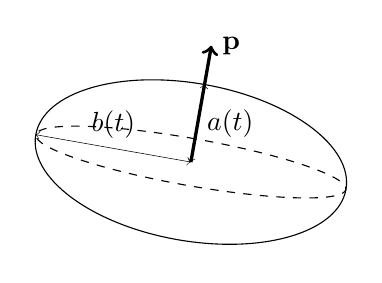
\begin{tikzpicture}[rotate=80]
        \draw(0,0) ellipse (1 cm and 2 cm);
        \draw[dashed](0,0) ellipse (0.3 cm and 2 cm);
        \draw[<->,very thin](0,0) --++ (1,0)node[midway,right]{$a(t)$};
        \draw[->,very thick](0,0) --++ (1.5,0)node[right]{$\textbf{p}$};
        \draw[<->,very thin](0,0) --++ (0,2)node[midway,above]{$b(t)$};
    \end{tikzpicture}
    \hfill
    \caption{Scheme of an  oblate spheroid oriented along the unit vector \textbf{p}.}
    \label{fig:scheme2}
\end{figure}
We consider in this problem an oblate spheroid with a time dependent aspect ratio $\chi = a(t)/b(t)$ oriented along the unit vector \textbf{p}, see \ref{fig:scheme2}.
In this context an equation describing the droplets surface can be found in the reference frame of the droplets, namely, 
\begin{equation}
    \mathscr{F}
    = \textbf{r}\cdot \textbf{H}\cdot \textbf{r} - a_0^2 = 0 
    \label{eq:F_def}
\end{equation}
where \textbf{H} is a symmetric traceless tensor such that $\textbf{H} = \textbf{pp} (a_0/a(t))^2 + (\textbf{I}- \textbf{pp})(a_0/b(t))^2$. 

We consider a mono disperse suspension of droplet with constant mass. 
The objective of this section is to derive constitutive equations to predict the mean orientation, and mean aspect ratio of the droplet. 

\subsubsection{Particle's internal motion}

In the first place we assume a linear homogeneous particle internal motion, such as, 
\begin{equation}
    \textbf{w}_2^0(\textbf{x}_\alpha+ \textbf{r})
    = 
    + \textbf{r} \cdot \textbf{D}_\alpha
    = 
    \bm{\omega}_\alpha \times \textbf{r} 
    + \textbf{r} \cdot \textbf{E}_\alpha
\end{equation}
where $\bm{\omega}_\alpha$ is the angular velocity of the particle, $\textbf{E}_\alpha$ is the mean deformation gradient. 
% Note that the second rank tensor $\textbf{U}_\alpha = \bm{\}$
To respect the mass conservation condition, i.e. $\div \textbf{w}_2^0 =0$, The mean gradient deformation $\textbf{E}_\alpha$ has to respect the conditions : $\textbf{E}_\alpha:\textbf{I}=0$. 
The assumption of linear internal motion is wrong for droplets and bubbles were we are clearly in presence of internal motions. 
However, for now these motions will be discarded. 

\subsubsection{Fundamental properties}

We now compute the mass, moment of mass and moment of momentum of this particle. 
The volume of an ellipsoid reads as, 
\begin{align}
    v_\alpha
    = \frac{4}{3}\pi a b^2
    = \frac{4}{3}\pi \chi  b^3
    \label{eq:volume_def}
\end{align}
Before going further we must say that the two radius $a(t)$ and $b(t)$ are actually dependent since one must preserve the total mass of the particle. 
We recall that we are in the context of mono disperse suspension such that the volume of the particles $v_\alpha$ is actually known, Thus, 
\begin{equation*}
    a(t) 
    = \frac{3 v_\alpha}{4 \pi b^2(t)}
    = \frac{r_0^3}{ b^2(t)}
    \Leftrightarrow
    b^2(t) 
    = \frac{r_0^3}{ a(t)}
\end{equation*}
Where $r_0$ is the radius of the sphere of same volume such as $v_\alpha = \frac{4}{3}\pi r_0^3$. 
Also, it might be useful to compute the relation between the derivative of the radius,  
\begin{equation*}
    \ddt v_\alpha 
    % = \ddt \frac{4}{3}\pi a b^2
    = \frac{4}{3}\pi \dot{a}(t) b^2(t)
    + \frac{8}{3} \pi {a}(t) b(t) \dot{b}(t)
    = 0 
    \Leftrightarrow
     \dot{a}(t)
    =  
    - 2 \frac{a(t)}{b(t)}  \dot{b}(t)
    % \Leftrightarrow
\end{equation*}
Which means that the derivative of both radius are related to twice the aspect ratio. 

The second moment of mass is somewhat more complicated to compute, we have, 
\begin{align*}
    \mathcal{M}_{\alpha,ij}
    = \int r_ir_j dxdydz
\end{align*}
At this stage we would like to compute the integral in spherical coordinate, thus we introduce the change of variables, 
\begin{align*}
    x' = x/a 
    && y' = y/b 
    && z' = z/b 
\end{align*}
By assuming that the spheroid is aligned with the $z$ axis and centered at the origin we get, 
\begin{align*}
    \mathcal{M}_{\alpha,zz}
    = a(t)^3 b(t)^2 \int z'z' dx'dy'dz'
\end{align*}
switching in spherical coordinate yields 
\begin{align*}
    \mathcal{M}_{\alpha,zz}
    = a(t)^3 b(t)^2 \int_0^1 \int_0^{2\pi}\int_0^\pi r^4 \cos^2\phi \sin\phi d\phi d\theta dr
    = a(t)^3 b(t)^2 \frac{1}{5}\frac{4}{3} \pi
    = v_\alpha \frac{a^2(t)}{5}\\
    \mathcal{M}_{\alpha,xx}
    = a(t) b(t)^4 \int_0^1 \int_0^{2\pi}\int_0^\pi r^4 \sin^3\phi\cos^2\theta d\phi d\theta dr
    = a(t) b(t)^4
    \frac{1}{5}
     \frac{4}{3}
     \pi
     =v_\alpha \frac{b^2(t)}{5}
\end{align*}
In a more general manner one can define the tensor $\mathcal{M}_\alpha$ in the laboratory reference frame using the orientation tensor \textbf{p}, such that, 
\begin{equation}
    5 \frac{\mathcal{M}_{\alpha,ij}}{v_\alpha}
    = p_i p_j 
    a^2(t) 
    + (\delta_{ij} - p_ip_j) b^2(t)
    = H_{ij}^{-1}
    \label{eq:M_alpha_def}
\end{equation} 
In light of \ref{eq:M_alpha_def}we reduced the description of any particle in our flow to four parameters, the 3 components of \textbf{p}, and the radius $a(t)$. 
It might be useful to make the inertia tensor dimensionless by dividing both sides by $r_0$, which gives, 
\begin{equation}
    5 \frac{\mathcal{M}_{\alpha,ij}}{v r_0^2}
    = p_i p_j 
    e_{||}^2(t) 
    + (\delta_{ij} - p_ip_j) 
    e_\bot^2(t) 
    \label{eq:M_alpha_def2}
\end{equation} 
Note that since $ab^2 =r_0^3$ the deformation are related through $e_\bot = \frac{b}{a}r e_{||} =\frac{b^3}{r^2} e_{||} $


Now let's compute the first moment of momentum $\mathcal{P}_\alpha$, it reads, 
\begin{align*}
    \mathcal{P}_{\alpha,ij}
    = \int r_i w_{2,j}^0 d\Omega
    = D_{\alpha,jk} \mathcal{M}_{\alpha,ki}
    = \epsilon_{jkl} \omega_{\alpha,k} \mathcal{M}_{\alpha,il}
    +  E_{\alpha,jk} \mathcal{M}_{\alpha,ik}
\end{align*}
Taking the double contracted product with $\epsilon_{mij}$ of the moment of momentum yield the angular momentum equation, 
\begin{align*}
    \mu_{\alpha,m}
    = \epsilon_{mij}\mathcal{P}_{\alpha,ij}
    = \epsilon_{jmi} \epsilon_{jkl} \omega_{\alpha,k} \int r_i r_l  d\Omega
    +  \epsilon_{mij} E_{\alpha,jk} \int r_i r_k  d\Omega\\
    = (\delta_{mk}\mathcal{M}_{\alpha,ll} - \mathcal{M}_{\alpha,mk}) \omega_{\alpha,k}
    +  \epsilon_{mij} E_{\alpha,jk} \int r_i r_k  d\Omega\\
    = \mathcal{I}_{\alpha,mk} \omega_{\alpha,k}
    +  \epsilon_{mij} E_{\alpha,jk} \mathcal{M}_{\alpha,ik}\\
\end{align*}
The second contribution of the angular momentum would vanish if the particles where spherical. 
Lastly, the symmetric part of the moment of momentum reads, 
\begin{align*}
    2\mathcal{S}_{\alpha,ij}
    = \epsilon_{jkl} \omega_{\alpha,k} \mathcal{M}_{\alpha,il}
    + \epsilon_{ikl} \omega_{\alpha,k} \mathcal{M}_{\alpha,jl}
    +  E_{\alpha,jk} \mathcal{M}_{\alpha,ik}
    +  E_{\alpha,ik}  \mathcal{M}_{\alpha,jk}
\end{align*}

\subsubsection*{Evolution equation of a single particle shpae.}

We first start by the kinetic equations.  
In view of the previous expression the evolution equation of the momentum tensor is,  
\begin{equation*}
    \ddt {\mathcal{M}_{\alpha,ij}}
    + \epsilon_{jlk} \omega_{\alpha,k} \mathcal{M}_{\alpha,il}
    - \epsilon_{ikl} \omega_{\alpha,k} \mathcal{M}_{\alpha,jl}
     =  E_{\alpha,jk} \mathcal{M}_{\alpha,ik}
     +  E_{\alpha,ik}  \mathcal{M}_{\alpha,jk}
     \label{eq:dt_M_alpha_bis}
\end{equation*}
On the left-hands-side of \ref{eq:dt_M_alpha_bis} we clearly identify the Jaumann derivative rotating with the vorticity.
To close this equation one may relate the mean ambient flow variables to the particles angular rotation and stretching rate. 
This however this is only possible considering pure stokes flow.

\subsubsection*{Equation for the bulk stress}

The equivalent stress can be formulated as, 
\begin{equation*}
    \bm{\sigma}
    = 
    \phi_1 \bm{\sigma}_1
    + \phi_2 \bm{\sigma}_2
    + \phi_I \bm{\sigma}_I
    \label{eq:sigma_def}
\end{equation*}
The particle phase stress can be reduced to its first moment, $\phi_2 \bm{\sigma}_2 = \pOavg{\bm{\sigma}_2^0}$.
Additionally, we adopt the approximation of homogeneous deformation so that the rate of strain within the particle equal its mean deformation $\textbf{E}_\alpha$.
Thus, we can write 
\begin{equation*}
    \phi_2 \bm{\sigma}_2 
    = - \phi_2 p_2
    + \phi_2 \mu_2 \textbf{E}_p
\end{equation*}
The fluid phase stress can be formulated as $\phi_1 \bm{\sigma}_1 =  - \phi_1 p_1 + \mu_1 \textbf{e} - \mu_1 \phi_2 \textbf{e}_2$.
Likewise, since we considered a constant strain within the particles we can write $\phi_2\textbf{e}_2 = \phi_2 \textbf{E}_p$ in homogeneous medium.   
The previous expression of the averaged stress yields, 
\begin{equation*}
    \bm{\sigma}
    = 
    - p 
    + \mu_1 \textbf{e} 
    + (\mu_2 - \mu_1) \phi_2 \textbf{E}_p
    + \phi_I \bm{\sigma}_I
    \label{eq:sigma_def}
\end{equation*}
In the above stress equation $\bm{\sigma}_I$ is still unknown and must be closed. 
While the others parameters can be easily linked to our problem variable. 

We recall that in homogeneous flows, $\phi_I \bm{\sigma}_I \approx \gamma\pSavg{\textbf{I}-\textbf{nn}}$. 
Let decompose this tensor into an isotropic tensor i.e. $\gamma\pSavg{\textbf{I}-\textbf{nn}} : \textbf{I} \frac{1}{3}I = \gamma\pSavg{} \frac{2}{3} \textbf{I}$ and an anisotropic tensor which reads, $\phi_I \bm{\sigma}_I \approx \gamma\pSavg{\frac{1}{3}\textbf{I}-\textbf{nn}}$.  
Therefore, to close this term one must compute the curvature of the particles. 
The first moment of surface tension stress can be computed analytically following \citep{nadim1996concise} for the curvature computation.
The analytical expression of the ellipse surface will enable us to compute the curvature of each particle.  
Let $\mathscr{F}(\textbf{x},t) = 0$ be the equality representing the ellipsoidal shape of the particle. 
First, the normal pointing in the direction of positive $\mathscr{F}$ at the interface, can be computed as, 
\begin{equation*}
    \textbf{n} = \frac{\grad \mathscr{F}}{(\grad \mathscr{F}\cdot \grad \mathscr{F})^{1/2}} \;\;\text{ on }\;\; \mathscr{F} = 0.  
\end{equation*}
Noticing that $\grad \mathscr{F} = 2\textbf{H}\cdot \textbf{r}$ one obtain, 
\begin{equation*}
    \bm{\sigma}_I^0 =\gamma\left[
    \textbf{I} - \frac{ \textbf{HH} :  \textbf{rr}}{ (\textbf{H}\cdot  \textbf{H}\cdot \textbf{rr})} \right]
\end{equation*}
We recall that this quantity drives the stress jump at the interface. 
As it is expected this stress jump is axis symmetric around the particle main axis. 
Besides, it is maximum at the poles and minimum at the equator of the particle. 
It is then possible to compute the integral of the stress by direct integration in the reference frame of the ellipsoid principal axes. 
The exact result yields, 
\begin{equation*}
    \gamma\pSavg{\textbf{I}-\textbf{nn}}
    = \gamma \left[
        \frac{2}{3} s_\alpha \textbf{I}
        + S (\textbf{I}-\textbf{pp}) -2S\textbf{pp}
        \right]
\end{equation*}
where the first component correspond to the isotropic part of the surface stress, and the second component to the deviatoric part of the surface stress. 
Note that the deviatoric part of this tensor is function of one unique coefficient, $S$ due to the axis symmetrical nature of the droplets. 
Exact solution can be given in terms of the small deformation parameter $e_\bot = b/r$. 
Then an approximation can be deduced for the $e -1 \ll 1$, it gives,
\begin{align*}
    s_\alpha 
    = 4\pi r^2 \left[\frac{e_\bot^2}{2} + \frac{\ln\left(\sqrt{{e_\bot^6}-1}+{e_\bot^3}\right)}{2e_\bot\sqrt{e_\bot^6-1}}\right]
    = 4 \pi r^2 + \frac{24 v }{5 r} (e_\bot-1)^2\\
    S = \frac{4}{3} \pi r^2 \left[
    \frac{\left( \frac{1}{4} - e_\bot^6\right)  \log{\left( \sqrt{e_\bot^6-1}+{e_\bot^3}\right) } }
    { e_\bot  \left( e_\bot^6- 1\right)^{3/2} }
    +  \frac{e_\bot^2\left( e_\bot^6+  \frac{1}{2}\right)}{2\left( e_\bot^6- 1\right)}  \right]
    \approx 
    \frac{8 v}{5 r}(e_\bot-1) + \frac{12 v }{35r}(e_\bot-1)^2 \ldots
\end{align*}
Regarding the expression of the surface of the spheroid, it can be noted that the function within bracket tends to $1$ for $e=1$ leaving us with $s_\alpha = 4\pi r^2$ which is the surface of the sphere. 
Then, it slowly increases when $e$ is either superior or inferior to $1$. 

Equally, the results can be expressed in terms of the deformation parameter $e_{||} = a/r$ in which case the previous results give at the second order in $e_\bot-1$ the following expression, 
\begin{align*}
    s_\alpha 
    \approx 4 \pi r^2 + \frac{6 v }{5 r} (e_{||}-1)^2 \ldots\\
    S 
    \approx 
    - \frac{4 v}{5 r}(e_{||}-1) + \frac{24 v }{35r}(e_{||}-1)^2 \ldots
\end{align*}
Noticing that the Hooke strain tensor $\textbf{C} = (e_{||}-1) \textbf{pp} + (e_\bot-1)(\textbf{I}- \textbf{pp})$, thus one can finally write,
\begin{align*}
    \pSavg{\bm\sigma_I^0}
    = \frac{\gamma v 2}{r} \left[
        1  + \frac{1}{20 }\textbf{C}:\textbf{C}\right] \textbf{I}
        - \frac{\gamma v}{35 r} \left[ 28 \textbf{C}_{-\textbf{I}}
        + 4[\textbf{C}_{-\textbf{I}}\cdot \textbf{C}_{-\textbf{I}} + 15 (\textbf{C}_{-\textbf{I}}:\textbf{pp})^2\textbf{pp}]
        \right]
\end{align*}
This gives the surface stress tensor up to the second order terms in accuracy. 
To our knowledge this has never been proposed. 
Retaining only the first order terms this expression shows that the drop behave as stressed material. 
Indeed, at rest the Laplace pressure is still present. 

It might be interesting to relate teh inertia tensor $\mathcal{M}_\alpha$ and \textbf{C}. 
Indeed, it can be shown that, 
\begin{equation}
    \mathcal{M}_\alpha
     = \frac{v r^2}{5}\left(\textbf{C} + \textbf{I}\right)
\end{equation}
Or equally, 
\begin{equation}
    \textbf{C}
     = \frac{5}{vr^2}\mathcal{M}_\alpha - \textbf{I}
\end{equation}
It is now trivial to re derive \citet{goddard1967nonlinear} equations of motions. 


The only unknown is now the particle strain rate $\textbf{E}_p$ and orientation tensor $\textbf{pp}$ and particle strain tensor \textbf{C} which is only one scalar function. 
\begin{itemize}
    \item Give the Laplace law for elongated bubbles 
    \item \tb{introduce the drop strain from the local strain as it is defined in solid mechanics.}
    \item \tb{TRY TO GET THE SAME EQ as godard}
    \item \tb{DERIVE STRESS EQ WITH C}
    \item The conclusion will be that we could generalize the transport equations or C easli  however we cannot actually close the equaitons for now !! ! 
\end{itemize}

\subsubsection*{Equation for the particles strain}

Additionally, using the first moment of momentum expression one can obtain an other expression for the particles internal stress, 
\begin{equation}
    \intS{ (\bm{\sigma}_I)_{ik}}
    +\intO{ (\bm{\sigma}_2^0)_{ik}}
    = 
    \intO{ \rho_2 
    (\textbf{w}_2^0\textbf{w}_2^0  )_{ik}
    }
    -\ddt \intO{ r_i (\textbf{u}^0_2)_k }
    +\intS{ 
     r_i (\bm{\sigma}_1^0 \cdot \textbf{n}_2)_{k}
    }
\end{equation}

\subsubsection*{Equation for the particle angular momentum}
\begin{equation*}
    \ddt \mu_p = t_p
\end{equation*}
% % In this section we propose to study two example. 
This objective is to demonstrate how to derive specific application from our general hybrid model. 
Secondly, we wish to point out in wish situation one needs or might not need the more than the zeroth order equation of the particle phase.

% \subsection{Solid axis symmetric particle suspension}

% Let's start by the second moment of mass averaged equation.
As a first example let examine the case of a mono-disperse axissymmetric suspension of solid particles, such as ellipsoid or cylinders.
Let the vector $\textbf{p}$ denote the unit vector representing the orientation of the particle along its main axis of inertia. 
Then, the second moment of mass can be written as $\mathcal{M}_{\alpha,ij} =  p_ip_j M_\alpha^{||} +  \delta_{ij} M_\alpha^\bot$, where $M_{\bot}$ and $M_{||}$ represent the coefficients corresponding to the principal directions of the particles' mass distribution.
It is well-established that at least the drag force exhibits a significant dependence on the orientation of the particle \citep{kim2013microhydrodynamics}.
Therefore, despite being a second-order moment, the particle field $\mathcal{M}_p$ is indispensable to close the mono-disperse axissymmetric suspension problem.
We will see that to determine the orientation of the particles one need to know about its angular velocity, which give the use to the equation for $\mathcal{P}_p$, equally.  


% \subsubsection{Single particle equations}

We first focus on the one particle dynamic before deriving the averaged equations. 
As stated above we assume the velocity of the dispersed phase to be of the form : $u_{2,i}^0(\textbf{x}_\alpha + \textbf{r}) = u_{i}^\alpha + \epsilon_{ijk} {\omega}_{j}^\alpha {r}_k$, with $\omega_{a}^\alpha$ the angular velocity of the particle $\alpha$ and $\epsilon$ the Levi-Cita symbol.
Injecting this definition of the velocity in \ref{eq:mu_def}, \ref{eq:S_def} and \ref{eq:E_def} one can re-write the moment of momentum skew-symmetric and symmetric part and the internal energy equation, of the particle as,
\begin{align}
    % \label{eq:S_def}
    2\mathcal{S}_{\alpha,ij}
    % = \Omega_{\alpha,jk} \mathcal{I}_{\alpha,ki} + \Omega_{\alpha,ik} \mathcal{I}_{\alpha,kj}
    = - \epsilon_{jak} \omega_a^\alpha \mathcal{I}_{ki}^\alpha
      - \epsilon_{ibk} \omega_b^\alpha \mathcal{I}_{kj}^\alpha
    % = 
    % M_\alpha^{||}  \left(
    %     \epsilon_{ikl} \omega_k 
    %     p_lp_j 
    %     +  \epsilon_{jkl} \omega_k 
    %     p_lp_i 
    % \right)
    \\
    % \label{eq:mu_def}
    \mu_{\alpha,i}
    % = 
    % \omega_{\alpha,j}(\mathcal{M}_{\alpha,kk} \delta_{\alpha,ij} - \mathcal{M}_{\alpha,ij})=
    % \omega_j \left[
    %     \delta_{ji} (M_\alpha^{||} + 2M_\alpha^\bot)
    %     - p_jp_i M_\alpha^{||} 
    % \right]
    =  \mathcal{I}_{ij}^\alpha \omega^\alpha_j\\
    2W_\alpha 
    = \omega^\alpha_k\omega^\alpha_l \mathcal{I}_{kl}^\alpha
\end{align}
Under this form notice that the angular momentum is the product of the angular velocity $\omega_{\alpha,i}$ times $\mathcal{I}_{ik}^\alpha = (\mathcal{M}_{kk}^\alpha \delta_{ij} - \mathcal{M}_{ij}^\alpha)$ which is consistent with the definition of the moment of inertia used in solid mechanics.
In fact, it has been found  more practical to express the following equation with $\mathcal{I}_\alpha$ rather than with $\mathcal{M}_\alpha$. 
Thus, in this section we express all closure and equation with respect to $\mathcal{I}_\alpha$
Now we make use of the preceding definition to rewrite the first moment of mass, angular momentum and internal energy equation, i.e. \ref{eq:dt_M_alpha}, \ref{eq:dt_P_alpha} and \ref{eq:dt_w2_alpha}, gives directly, 
\begin{align}
    \label{eq:dt_I_alpha}
    \ddt \mathcal{I}_{ij}
    = - \epsilon_{jak} \omega_a^\alpha \mathcal{I}_{ki}^\alpha + 
    - \epsilon_{ibk}   \omega_b^\alpha \mathcal{I}_{kj}^\alpha\\
    \label{eq:dt_Iomega_alpha}
    \ddt (\mathcal{I}_{ij}^\alpha \omega_j^\alpha)
    = t^\alpha_i\\
    \label{eq:dt_Iomegaomega_alpha}
    \frac{1}{2}\ddt (\omega^\alpha_k\omega^\alpha_l \mathcal{I}_{kl}^\alpha)
    = \omega_k t^\alpha_k. 
\end{align}
As, can be seen here the dependence of the inertia matrices with time induce a significant complication to the problem. 
Firstly we must keep track of the evolution of the inertia matrices which add one supplementary equation. 
Secondly, the angular momentum and angular kinetic energy of the particle is not function solely of the angular velocity but also on its own inertia matrices. 
Which will add difficulty to unpair to angular velocity from the inertia matrix in the averaged equation. 

% \tb{maybe add the heat issipation}
% It will be useful in the following derivation to have an equation for $\omega_i^\alpha$, manipulating the equation of angular momentum with the use of the equation of evolution of the inertia matrix we obtain, 
% \begin{equation}
%     \ddt (\omega_i^\alpha)
%     = (\mathcal{I}^\alpha)_{ik}^{-1}(  
%         t^\alpha_k
%     -  \mathcal{S}_{kl}^\alpha\omega_l^\alpha
%     )
% \end{equation}
% Taking the dot product of this equation with $\omega_j^\alpha$ and adding its transpose in the indices $ij$ gives, 
% \begin{equation}
%     \ddt (\omega_i^\alpha\omega_j^\alpha)
%     = 
%     \omega_j^\alpha
%     (\mathcal{I}^\alpha)_{ik}^{-1}(  
%         t^\alpha_k
%     -  \mathcal{S}_{kl}^\alpha\omega_l^\alpha
%     )
%     + \omega_i^\alpha
%     (\mathcal{I}^\alpha)_{jk}^{-1}(  
%         t^\alpha_k
%     -  \mathcal{S}_{kl}^\alpha\omega_l^\alpha
%     )
% \end{equation}

% Also, notice that the stress within the particle is supposed to be unknown. 
% Indeed, we considered rigid body motion inside the particles.
% However, it is still possible to evaluate the stress using the stretch of momentum equation which in this case yields, 
% \begin{equation*}
%     \intO{(\sigma_2^0)_{ij}}
%     = 
%     - \ddt \mathcal{S}^\alpha_{ij}
%     + \epsilon_{iab}\epsilon_{ibd}\omega_{b}^\alpha\omega_{d}^\alpha(
%         \frac{1}{2}\mathcal{I}_{kk}\delta_{ac}
%         - \mathcal{I}^\alpha_{ac} )
%     + S^\alpha_{ij}.
%     \\
% \end{equation*}
% Therefore, the stress can be computed conditionally on the knowledge of the angular velocity and acceleration of the particle, which can be determinate by solving the previous equations. 
% It is then possible to validate the hypothesis of deformable particle  upon the knowledge of the material body law. 

% Finally, in the perspective of deriving an equation for the covariance of the translational motion and the orientation we multiply the equation of $\mathcal{I}_{ij}^\alpha$ by $u_k^\alpha$ and the equation of $u_k^\alpha$ by $\mathcal{I}_{ij}^\alpha$, which gives us get the following equation,
% \begin{equation*}
%     \ddt (\mathcal{I}_{ij}^\alpha u_k^\alpha)
%     =
%     u_k^\alpha
%     \ddt \mathcal{I}_{ij}^\alpha
%     + \mathcal{I}_{ij}^\alpha \ddt u_k^\alpha
%     = u_k^\alpha \mathcal{S}_{ij}^\alpha
%     +  \mathcal{I}_{ij}^\alpha g_k
%     +  \mathcal{I}_{ij}^\alpha f_k^\alpha/m^\alpha
% \end{equation*}

% \subsubsection{Averaged equation for the fluid phase}

% It is somewhat simpler to first modify the fluid phase equations. 
% Indeed, among the 4 equations to be solved only the terms involving the internal velocity will be explicitly modified.  
% These terms appear in \ref{eq:dt_hybrid_k1}, under the form $\pSavg{{\textbf{rw}_2^0\times\bm{\sigma}_1^0 \cdot \textbf{n}_2}}$, where we substitute $\textbf{w}$ for the expression of a solid particle velocity field. 
% Substituting these terms into the pseudo turbulent energy equation gives, 
% \begin{multline*}
%     \pddt (\phi_1\rho_1k_1)  
%     + \div (
%         \phi_1\rho_1k_1\textbf{u}_1
%         + \textbf{q}_1^\text{k} 
%         )
%     = 
%     - \avg{\chi_1\bm{\sigma}_1^0 : \grad \textbf{u}_1^0}
%     - \bm{\sigma}_1^\text{eq} : \grad \textbf{u}_1
%     + (\textbf{u}_1 - \textbf{u}_p)
%     \cdot \pSavg{{\bm{\sigma}_1^0 \cdot \textbf{n}_2}}\\
%     - \pavg{ \textbf{u}^{\alpha'} \cdot \intS{  \bm{\sigma}_1^0 \cdot \textbf{n}_2}}
%     - \bm{\omega}_{p} \cdot  \pavg{\intS{\textbf{r}\times\bm{\sigma}_1^0 \cdot \textbf{n}_2}}
%     - \pavg{\bm{\omega}^{'}_\alpha  \cdot \intS{\textbf{r} \times \bm{\sigma}_1^0 \cdot \textbf{n}_2}}
%     % \pSavg{\textbf{r}\textbf{w}^0_2 \cdot \textbf{r}\bm{\sigma}_1^0 \cdot \textbf{n}_2}_l
% \end{multline*}
% with,
% \begin{multline*}
%     \textbf{q}_1^\text{k}
%     = \rho_1 \avg{\chi_1 \textbf{u}_1' k_1} 
%     - \avg{\chi_1 \textbf{u}_1' \cdot \bm{\sigma}_1^0}
%     + (\textbf{u}_1 - \textbf{u}_p)\cdot
%     \pSavg{{\textbf{r}\bm{\sigma}_1^0 \cdot \textbf{n}_2}}
%     \\
%     - \pavg{ \textbf{u}_\alpha' \cdot \intS{ \textbf{r} \bm{\sigma}_1^0 \cdot \textbf{n}_2}}
%     - \epsilon_{ijk} \omega_{p,j} \pavg{ \intS{\textbf{rr}\bm{\sigma}_1^0 \cdot \textbf{n}_2}}_{kli}
%     - \epsilon_{ijk}\pavg{\omega^{\alpha'}_{j}  \intS{\textbf{rr}\bm{\sigma}_1^0 \cdot \textbf{n}_2}}_{kli}
% \end{multline*}
% Now, we clearly see appear the mean and fluctuating work due to the rotational motion of the particles. 
% Which are the product of the angular velocities times the torque on the surface of the particles. 
% Similar comments can be made for the flux term were we see appear the work of the second moments of the surface traction with the angular velocity. 

% By the assumption of solid particle motion we already reformulated the closure terms of the form $\pSavg{{\textbf{rw}_2^0\times\bm{\sigma}_1^0 \cdot \textbf{n}_2}}$ surface traction tensor which were already present in the problem. 
% Nevertheless, we still now need to find additional closure related to the angular velocity covariance with the torque. 

% \begin{align*}
%     \pSavg{\textbf{w}^0_2\cdot \bm{\sigma}_1^0 \cdot \textbf{n}_2}
%     =
%     \epsilon_{ijk}\omega_{p,j}  \pavg{\intS{\textbf{r}\bm{\sigma}_1^0 \cdot \textbf{n}_2}_{ki}}
%     + \epsilon_{ijk}\pavg{{\omega}^{\alpha'}_{j}  \intS{\textbf{r}\bm{\sigma}_1^0 \cdot \textbf{n}_2}_{ki}}\\
%     \pSavg{\textbf{r}\textbf{w}^0_2 \cdot \textbf{r}\bm{\sigma}_1^0 \cdot \textbf{n}_2}_l
%     =
%     \epsilon_{ijk} \omega_{p,j} \pavg{ \intS{\textbf{rr}\bm{\sigma}_1^0 \cdot \textbf{n}_2}_{kli}}
%     + \epsilon_{ijk}\pavg{\omega^{\alpha'}_{j}  \intS{\textbf{rr}\bm{\sigma}_1^0 \cdot \textbf{n}_2}_{kli}}
% \end{align*}


\subsubsection{Orientation equation in stoke regime.}

Averaging the second-order moment of mass yields, $n_p \mathcal{M}_p =  \textbf{A}_p (M_p^{||} - M_p^\bot) +  \textbf{I} M_p^\bot$ where $\textbf{A}_p$ is the orientation tensor defined as $\textbf{A}_p = \avg{\delta_\alpha\textbf{pp}}$.
Then, let's express the internal motion of a solid particle by : $\textbf{u}_2(\textbf{x}_\alpha) = \textbf{u}_\alpha + \textbf{r}\times \omega_\alpha$ where $\omega_\alpha$ represents the angular velocity of the particle.
It follows the expression of the stretching of momentum : $\mathcal{S}_\alpha = (M_\alpha^{||} - M_\alpha^\bot) \left(
    \omega_\alpha \times
    \textbf{pp}
    + \textbf{pp} \times \omega_\alpha
\right)$. 
Subsequently,  we can easily derive the transport equation for $\textbf{A}$ by averaging \ref{eq:dt_M_alpha} and using the previous expressions for $\mathcal{M}_\alpha$ and $\mathcal{S}_\alpha$.
The resulting equation is given by~:
\begin{equation}
    \pddt (n_p\textbf{A})
    + \div (
        n_p\textbf{u}_p\textbf{A}_p
        + \mathbf{\Sigma}
        )
    =
    \pavg{\textbf{pp} \times \omega_\alpha}
    + \pavg{\omega_\alpha \times \textbf{pp}},
    % + \pnavg{\textbf{pp}' \times \omega_\alpha'}
    % +\pnavg{\omega_\alpha' \times \textbf{pp}'}
    \label{eq:avg_dt_M_alpha}
\end{equation}
where $\mathbf{\Sigma} = \pavg{\textbf{u}'_\alpha(\textbf{pp})'}$ is the covariance term between the fluctuation of the velocity and the orientation tensor.
We recall that the definition of the fluctuation notation is provided by the expression from \ref{eq:def_fluctu}.
At this stage we need to find closure for both terms on the RHS of \ref{eq:avg_dt_M_alpha}. 
Therefore, we assume torque free rigid particle in to Stokes flow, where we can utilize Jeffery's equation \citep{guazzelli2011}.
It reads,
\begin{equation}
    \omega_\alpha \times \textbf{p}
    = \mathbf{\Omega}\cdot\textbf{p}
    + \beta\left(
        \textbf{E}\cdot \textbf{p}
        - \textbf{E} : \textbf{ppp}
    \right),
    \label{eq:jefferey}
\end{equation}
with $\textbf{E}$ and $\mathbf{\Omega}$ being the symmetric and antisymmetric parts of the bulk velocity gradient, respectively, such that $\grad\avg{\textbf{u}}=\textbf{E}+\mathbf{\Omega}$.
The coefficient $\beta$  is a constant related to the aspect ratio of the particle.
Finally, by substituting the RHS terms of \ref{eq:avg_dt_M_alpha}, by using \ref{eq:jefferey}, we arrive at the closed form of the second moment of mass equation~:
\begin{equation}
    \pddt \textbf{A}
    + \div (
        \pnnavg{\textbf{u}_\alpha}\textbf{A}
    )
    =
    \mathbf{\Omega} \cdot \textbf{A}
    - \textbf{A} \cdot \mathbf{\Omega}
    + \beta\left[
        \textbf{E} \cdot \textbf{A}
        -\textbf{A} \cdot \textbf{E}
        - \textbf{E} : \mathbb{A}
    \right]
    - \div \mathbf{\Sigma}
    \label{eq:hybrid_avg_dt_pp}
\end{equation}
where the fourth-order tensor $\mathbb{A}$, is defined as $\mathbb{A} = \pavg{\textbf{pppp}}$.
In this expression we removed the fluctuation terms, but they must appear and they are surly not negligible. 
In \citet{wang2008objective} they derive \ref{eq:hybrid_avg_dt_pp} by the means of kinetic theory, based on \ref{eq:jefferey} and the fact that $\ddt \textbf{p} = \omega_\alpha \times \textbf{p}$ (Equation (3) of their article).
Their equation is similar to \ref{eq:hybrid_avg_dt_pp} except that their employ a phenomenological closure for the term, $\div \mathbf{\Sigma}$, which account for particles interactions \tb{je pense que c'est ca mais pas sur}.
Anyhow, we showed how it is possible to derive the orientation tensor conservation equation, commonly used in fiber field theory, from the second-order moments of mass's equation. 
However, \ref{eq:jefferey} is valid in low inertial regime only. 
Therefore, it is indispensable to consider a more general framework when working with inertial particles. 

\subsubsection{Averaged equation for the particle phase}

Now let's turn our attention to the particle phase equations in inertial form. 
We first introduce the average of the inertia matrix, angular momentum and internal energy as,
\begin{align}
    \label{eq:Sp_def}
    2(\mathcal{S}_{p})_{ij}
    = - \epsilon_{jak} \omega_{p,a} \mathcal{I}_{p,ki}
    - \epsilon_{ibk}   \omega_{p,b} \mathcal{I}_{p,kj}
    - \epsilon_{jak} k_{p,kia}^{\mathcal{I}\omega} 
    - \epsilon_{ibk} k_{p,kjb}^{\mathcal{I}\omega}
    \\
    \label{eq:mup_def}
    \mu_{p,i}
    = \mathcal{I}_{p,ij} \omega_{p,j}
    + k_{p,ijj}^{\mathcal{I}\omega}
    \\
    \label{eq:Wp_deformations}
    2 W_p 
    = 
    {\omega}_{p,i}{\omega}_{p,j} \mathcal{I}_{p,ij}
    % \omega_{p,i}\mu_{p,i}
    + \mathcal{I}_{p,ij} {k}^{ww}_{p,ij}
    + 2 {\omega}_{p,i} {k}_{p,ijj}^{\mathcal{I}\omega}
    + k^{Iww}_p
\end{align}
where we introduced the following fluctuating quantities, 
\begin{align*}
    n_p(\textbf{k}_p^{\mathcal{I}\omega})_{ijk}
    = 
    \pavg{\mathcal{I}^{\alpha'}_{ij} \omega^{\alpha'}_k}
    && n_p (k_p^{\omega\omega})_{ij}
    = 
    \pavg{\omega^{\alpha'}_i \omega^{\alpha'}_j}
    && n_p{k}_p^{\mathcal{I}\omega\omega}
    = 
    \pavg{\mathcal{I}^{\alpha'}_{ij} \omega^{\alpha'}_i\omega^{\alpha'}_j}
\end{align*}
Due to the covariance terms, the problem which contained only two unknown at the particle scale, i.e. $\mathcal{I}_\alpha$ and $\bm{\omega}_\alpha$, now contains 5 unknown on the macroscopic scale, i.e. $\mathcal{I}_p$, $\bm{\omega}_p$, $\textbf{k}^{\mathcal{I}\omega}_p$,$\textbf{k}^{ww}_p$ and $\textbf{k}_p^{\mathcal{I}\omega\omega}$
We therefore, need to derive five equation to compute properly the angular momentum and internal fluctuating energy of the particle phase. 


Taking the particle average of \ref{eq:dt_I_alpha},\ref{eq:dt_Iomega_alpha} and \ref{eq:dt_Iomegaomega_alpha} yield the particle average equations for the averaged inertia matrix the angular momentum and the internal kinetic energy, 
\begin{align}
    \label{eq:dt_avg_Ip}
    \pddt (n_p\mathcal{I}_{p,ij})
    + \div (n_p\mathcal{I}_{p,ij} u_{p,k}
    + \mathcal{I}^\text{flux}_{p,ijk})
    = n_p \mathcal{S}_{p,ij},\\ 
    \label{eq:dt_avg_mup}
    \pddt (
    %     n_p \mathcal{I}_{p,ij} \omega_{p,j}
    % + n_p k^{\mathcal{I}\omega}_{p,ijj}
    n_p \mu_{p,i}
    )
    + \div (
        n_p \mu_{p,i}u_{p,k}
    %     n_p \mathcal{I}_{p,ij} \omega_{p,j} u_{p,k}
    % + k^{\mathcal{I}\omega}_{p,ijj} u_{p,k}
    +  \omega_{p,j} \mathcal{I}^\text{flux}_{p,ijk}
    + \mu_{p,ik}^\text{flux}
    )
    = n_p t_{p,i},\\
    \pddt (n_p W_p)
    + \div  (
        n_p W_p u_{p,k}
        + \omega_{p,i} \omega_{p,j}
        \mathcal{I}_{p,ij}^\text{flux}/2
        + \omega_{p,i}\mu_{p,ik}^\text{flux}
    + W_{p,k}^\text{flux}
    )
    = 
    n_p \omega_{p,k} t_{p,k}
    +  \pavg{\omega_k^{\alpha'} t^\alpha_k},
\end{align}
respectively. 
Also, within these averaged equations the correlation of the translational velocity and each of these quantities  appear under the form $(\ldots)^\text{flux}$ have the following expression, 
\begin{align*}
    n_p \mathcal{I}_{p,ijk}^\text{flux}
    = n_p k_{p,ijk}^{\mathcal{I}u}
    = 
    \pavg{\mathcal{I}^{\alpha'}_{ij} u_{k}^{\alpha'}}
    &&
    n_p \mu_{p,ik}^\text{flux}
    = 
    \pavg{\mathcal{I}^{\alpha'}_{ij} \omega^{\alpha'}_j u_{k}^{\alpha'}} 
    + \mathcal{I}_{p,ij} \pavg{u_k^{\alpha'}\omega_j^{\alpha'}}\\
    && n_p W_{p,k}^\text{flux}
    = \frac{1}{2}\mathcal{I}_{p,ij}
    \pavg{
        \omega_j^{\alpha'}
        \omega_i^{\alpha'}
        u_k^{\alpha'}
    }
    + \frac{1}{2}\pavg{
        \mathcal{I}_{ij}^{\alpha'}
        \omega_j^{\alpha'}
        \omega_i^{\alpha'}
        u_k^{\alpha'}
    }.
\end{align*}
At this stage all the fluctuating terms $k^{\ldots}$ can be considered as closure term or as terms to be solved thanks to a secondary transport equations in the same spirit as the pseudo turbulent equation for $k_p$.
Upon substituting $\mathcal{I}_p$ with the orientation vector $\textbf{pp}$ the reader can notice that \ref{eq:dt_avg_Ip} reveal being the equation for the orientation tensor $\pavg{\textbf{pp}}$ \citep{wang2008objective} which is widely used in the fiber suspension study. 
In the context of stokesian suspension the term appearing in the RHS of \ref{eq:dt_avg_Ip} is directly closed through the use of Jeffery's equation \citet{guazzelli2011}.
It leads to a closed equation for the orientation tensor in terms of the derivative of the mean flow field. 
In a more general context, to close the inertia tensor equation and compute the total angular momentum, one needs to obtain an equation for $k^{\mathcal{I}\omega}_{p,ijj}$. 
This is done by first taking the dot product of $\bm{\omega}_{p}$ with \ref{eq:dt_avg_Ip} on the index $j$, then subtracting this expression to \ref{eq:dt_avg_mup}.
This gives rise to an equation for the mean angular velocity and mean fluctuating part of the angular momentum, namely, 
\begin{align}
    \label{eq:dt_avg_kIp}
    \pddt (n_p\mathcal{I}_{p,ij}\omega_{p,j})
    + \div (n_p\mathcal{I}_{p,ij}\omega_{p,j} u_{p,k}
    + \omega_{p,j}\mathcal{I}^\text{flux}_{p,ijk})
    &= 
    n_p \mathcal{S}_{p,ij}\omega_{p,j}
    + \mathcal{I}_{p,ijk}^\text{flux}\grad \omega_{p,j}
    + \mathcal{I}_{p,ij}\pavg{\dot{\omega}^\alpha_j}
    \\
    \label{eq:dt_avg_kIp}
    \mathcal{I}_{p,ij}\left[
        \pddt (n_p\omega_{p,j})
        + \div (n_p\omega_{p,j} u_{p,k})
    \right]
    &= 
    \omega_{p,j}\div\mathcal{I}_{p,ijk}^\text{flux} 
    + \mathcal{I}_{p,ij}\pavg{\dot{\omega}^\alpha_j},
    \\
    \pddt (n_p k^{\mathcal{I}\omega}_{p,ijj})
    + \div (k^{\mathcal{I}\omega}_{p,ijj} u_{p,k}
    + \mu_{p,ik}^\text{flux}
    )
    &= 
    - n_p \mathcal{S}_{p,ij}\omega_{p,j}
    - \mathcal{I}_{p,ijk}^\text{flux}\grad \omega_{p,j}
    - \mathcal{I}_{p,ij}\pavg{\dot{\omega}^\alpha_j}
    + n_p t_{p,i},
\end{align}
respectively. 
The third term in the right hands side of this equation and the mean torque term eventually cancel out leaving only with fluctuating quantities. 
% Now let's turn our attention to the energy parts, 
% \begin{align*}
%     \pddt (n_p\mathcal{I}_{p,ij}\omega_{p,j}\omega_{p,i})
%     + \div (n_p\mathcal{I}_{p,ij}\omega_{p,j}\omega_{p,i} u_{p,k}
%     + \omega_{p,j}\omega_{p,i}\mathcal{I}^\text{flux}_{p,ijk})
%     = 
%     n_p \mathcal{S}_{p,ij}\omega_{p,j}\omega_{p,i}\\
%     + \mathcal{I}_{p,ijk}^\text{flux}\grad (\omega_{p,j}\omega_{p,i})
%     + \mathcal{I}_{p,ij}(
%         \omega_{p,i}\pavg{\dot{\omega}^\alpha_j}
%         +  \omega_{p,j}\pavg{\dot{\omega}^\alpha_i}
%     )
%     \\
%     \pddt (n_p \omega_{p,i}k^{\mathcal{I}\omega}_{p,ijj})
%     + \div (\omega_{p,i}k^{\mathcal{I}\omega}_{p,ijj} u_{p,k}
%     + \omega_{p,i}\mu_{p,ik}^\text{flux}
%     )
%     = 
%     - \omega_{p,i} n_p \mathcal{S}_{p,ij}\omega_{p,j}
%     - \omega_{p,i} \mathcal{I}_{p,ijk}^\text{flux}\grad \omega_{p,j}\\
%     - \omega_{p,i} \mathcal{I}_{p,ij}\pavg{\dot{\omega}^\alpha_j}
%     + \omega_{p,i} n_p t_{p,i}
%     + k^{\mathcal{I}\omega}_{p,ijj} \pavg{\dot{\omega}^\alpha_i}
%     + \mu_{p,ik}^\text{flux} \grad\omega_{p,i}
% \end{align*}
Subtracting from the energy equation half of \ref{eq:dt_avg_Ip} times $\omega_{p,i}\omega_{p,j}$, and \ref{eq:dt_avg_kIp} time $\omega_{p,i}$ gives us the last equation for the angular velocity covariance terms, namely, 
\begin{multline}
    \pddt (n_p (\mathcal{I}_{p,ij} k^{\omega\omega}_{p,ij}+k^{\mathcal{I}\omega\omega}_{p}))
    + \div  (
        n_p (\mathcal{I}_{p,ij} k^{\omega\omega}_{p,ij}+k^{\mathcal{I}\omega\omega}_{p}) u_{p,k}
    + W_{p,k}^\text{flux}
    )
    % = 
    % n_p \omega_{p,k} t_{p,k}
    % + \pavg{\omega_k^{\alpha'} t^\alpha_k} \\
    % + \omega_{p,i} n_p \mathcal{S}_{p,ij}\omega_{p,j}
    % + \omega_{p,i} \mathcal{I}_{p,ijk}^\text{flux}\grad \omega_{p,j}
    % + \omega_{p,i} \mathcal{I}_{p,ij}\pavg{\dot{\omega}^\alpha_j}
    % - \omega_{p,i} n_p t_{p,i}
    % - k^{\mathcal{I}\omega}_{p,ijj} \pavg{\dot{\omega}^\alpha_i}
    % - \mu_{p,ik}^\text{flux} \grad\omega_{p,i}\\
    % - \frac{1}{2} n_p \mathcal{S}_{p,ij}\omega_{p,j}\omega_{p,i}
    % - \frac{1}{2} \mathcal{I}_{p,ijk}^\text{flux}\grad (\omega_{p,j}\omega_{p,i})
    % - \frac{1}{2} \mathcal{I}_{p,ij}(
    %     \omega_{p,i}\pavg{\dot{\omega}^\alpha_j}
    %     +  \omega_{p,j}\pavg{\dot{\omega}^\alpha_i}
    % )\\
    = \\
    \pavg{\omega_k^{\alpha'} t^\alpha_k} 
    + \frac{n_p}{2}\omega_{p,i} \omega_{p,j} \mathcal{S}_{p,ij}
    % + \omega_{p,i} \mathcal{I}_{p,ijk}^\text{flux}\grad \omega_{p,j}
    % + \omega_{p,i} \mathcal{I}_{p,ij}\pavg{\dot{\omega}^\alpha_j}
    % - \omega_{p,i} n_p t_{p,i}
    - k^{\mathcal{I}\omega}_{p,ijj} \pavg{\dot{\omega}^\alpha_i}
    - \mu_{p,ik}^\text{flux} \grad\omega_{p,i}
    % - \frac{1}{2} n_p \mathcal{S}_{p,ij}\omega_{p,j}\omega_{p,i}
    % - \frac{1}{2} \mathcal{I}_{p,ijk}^\text{flux}\grad (\omega_{p,j}\omega_{p,i})
    % - \frac{1}{2} \mathcal{I}_{p,ij}(
    %     \omega_{p,i}\pavg{\dot{\omega}^\alpha_j}
    %     +  \omega_{p,j}\pavg{\dot{\omega}^\alpha_i}
    % )
    \label{eq:dt_avg_kpww}
\end{multline}
However, we can observe that the exchange term appearing in the fluid phase turbulent equation is also present here. 
Meaning that the correlation of the torque with the angular velocity makes the energy transfer between the fluid turbulent energy $k_1$ and the particles fluctuating motion $\mathcal{I}_{p,ij} k^{\omega\omega}_{p,ij}+k^{\mathcal{I}\omega\omega}_{p}$. 
It is now complicated to see how to isolate $k^{\omega\omega}_{p,ij}$ from $k^{\mathcal{I}\omega\omega}_{p}$ into two distinct equation ,however it is really needed ? 
In the specific case of solid spherical particles all the quantities involving the inertial matrix contribution vanish due to the frame independence.
Upon noticing that, compare \ref{eq:dt_avg_kpww} with Equation (9.28) of \citet[Chapter 9]{rao2008introduction}. 
Their equation, derived with the help of kinetic theory remain consistent with \ref{eq:dt_avg_kpww} however in the form of the hybrid model we clearly see which exchange terms communicate with which equations. 


% In order to isolate these terms we must derive the averaged equation for $(\omega\omega)$. 
% \begin{multline*}
%     \pddt (n_p \omega_{p,i}\omega_{p,j} 
%     +n_p k^{\omega\omega}_{p,ij})
%     + \div (n_p \omega_{p,i}\omega_{p,j}u_{p,k} 
%     +n_p k^{\omega\omega}_{p,ij}u_{p,k}
%     + \omega^\text{flux}_{p,ijk})
%     = \\
%     \pavg{\omega_j^\alpha
%     (\mathcal{I}^\alpha)_{ik}^{-1}(  
%         t^\alpha_k
%     -  \mathcal{S}_{kl}^\alpha\omega_l^\alpha
%     )}
%     + \pavg{\omega_i^\alpha
%     (\mathcal{I}^\alpha)_{jk}^{-1}(  
%         t^\alpha_k
%     -  \mathcal{S}_{kl}^\alpha\omega_l^\alpha
%     )}
% \end{multline*}
% Which upon multiplying by $\mathcal{I}_{p,ij}$ gives the last equations, 
% \begin{multline*}
%     \pddt (n_p \omega_{p,i}\omega_{p,j} \mathcal{I}_{p,ij}
%     +n_p k^{\omega\omega}_{p,ij}\mathcal{I}_{p,ij}
%     )
%     + \div (n_p \omega_{p,i}\omega_{p,j}u_{p,k}  \mathcal{I}_{p,ij}
%     +n_p k^{\omega\omega}_{p,ij}u_{p,k} \mathcal{I}_{p,ij}
%     + \omega^\text{flux}_{p,ijk} \mathcal{I}_{p,ij}
%     )
%     = \\
%     +\omega_{p,ijk}^\text{flux}\grad \mathcal{I}_{p,ij}
%     + 2 \mathcal{I}_{p,ij} 
%     \pavg{\ddt(\omega_i^\alpha\omega_j^\alpha)}
    % \\
    % \mathcal{I}_{p,ij}\pavg{\omega_j^\alpha
    % (\mathcal{I}^\alpha)_{ik}^{-1}(  
    %     t^\alpha_k
    % -  \mathcal{S}_{kl}^\alpha\omega_l^\alpha
    % )}
    % + \mathcal{I}_{p,ij}\pavg{\omega_i^\alpha
    % (\mathcal{I}^\alpha)_{jk}^{-1}(  
    %     t^\alpha_k
    % -  \mathcal{S}_{kl}^\alpha\omega_l^\alpha
    % )}
% \end{multline*}
% Now by subtracting from this equation the equation of the mean angular momentum gives us, 
% \begin{multline*}
%     \pddt (
%     n_p k^{\omega\omega}_{p,ij}\mathcal{I}_{p,ij}
%     )
%     + \div (
%     n_p k^{\omega\omega}_{p,ij}u_{p,k} \mathcal{I}_{p,ij}
%     + \omega^\text{flux}_{p,ijk} \mathcal{I}_{p,ij}
%     - \omega_{p,i}\omega_{p,j}\mathcal{I}_{p,ijk}^\text{flux}
%     )
%     = 
%     \omega_{p,ijk}^\text{flux}\grad \mathcal{I}_{p,ij}
%     + 2 \mathcal{I}_{p,ij} 
%     \pavg{\ddt(\omega_i^\alpha\omega_j^\alpha)}
%     \\
%     - n_p \mathcal{S}_{p,ij}\omega_{p,j}\omega_{p,i}
%     - \mathcal{I}_{p,ijk}^\text{flux}\grad (\omega_{p,j}\omega_{p,i})
%     - \mathcal{I}_{p,ij}(
%         \omega_{p,i}\pavg{\dot{\omega}^\alpha_j}
%         +  \omega_{p,j}\pavg{\dot{\omega}^\alpha_i}
%     )
% \end{multline*}
% which finally gives us the equation for the variance of the angular velocity. 

% Let's now derive a transport equation for the correlation tensor $\mathcal{I}^\text{flux}_{ijk}$. 
% \begin{equation*}
%     \pddt(n_p \mathcal{I}_{p,ij} u_{p,k} + \mathcal{I}^\text{flux}_{p,ijk})
%     + \div(\mathcal{I}_{p,ij} u_{p,k} u_{p,l}
%     + \mathcal{I}^\text{flux}_{p,ijk} u_{p,l}
%     + 
%     )
%     = 
%        \pavg{u_k^\alpha \mathcal{S}_{ij}^\alpha}
%     +  \pavg{\mathcal{I}_{ij}^\alpha }g_k
%     +  \pavg{\mathcal{I}_{ij}^\alpha f_k^\alpha/m^\alpha}
% \end{equation*}


% 

The conservation equations of mass and momentum, derived using \ref{eq:avg_dt_dq_alpha_tot} and \ref{eq:hybrid_avg_dt_chif} yield the same as the classical hybrid models derived in previous studies such as \citet{jackson1997locally} and \citet{zhang1997momentum} among others.
Therefore, it will not be discussed further as it does not contribute any relevant information to the current study.
Instead, in the subsequent analysis, we consider as known quantities : the fluid phase fraction $\phi_1$;
the particle number density $n_p$; the continuous phase-averaged velocity $\oneavg{\textbf{u}}$; and particle-average velocity $\pnnavg{\textbf{u}_\alpha}$. 
Which implies that the equations of conservation of mass and momentum for both the continuous and dispersed phase have been solved a priori, providing the values of these variables as known quantities.
Additionally, it also implies that the closure terms in the momentum equation, such as the mean interphase drag force $\pnnavg{\textbf{f}_\alpha}$ and others terms must be closed. 
However, those terms might depend on the higher moments of the particle phase, in which case it is crucial to provide a first-order moment equation. 
Therefore, the primary objective of this section is to emphasize the significance of the first-moment equations derived from \ref{eq:avg_dt_dQ_alpha_tot}, as they are often overlooked and underutilized in the literature.
In this section we stay succinct while providing the minimum level of understanding of the problem at hand.
Hence, we will not entirely deal with the closure problem of these first-order moments equations, but rather we focus on their derivation and interpretation. 

\subsection{Solid axis symmetric particle suspension}

% Let's start by the second moment of mass averaged equation.
Let's examine the scenario of a mono-disperse axissymmetric suspension of solid particles, such as ellipsoid or cylinders.
Let the vector $\textbf{p}$ denote the unit vector representing the orientation of the particle along its main axis of inertia. 
Then, the second moment of mass can be written as $\mathcal{M}_\alpha =  \textbf{pp} (M_\alpha^{||} - M_\alpha^\bot) +  \textbf{I} M_\alpha^\bot$, where $M_{\bot}$ and $M_{||}$ represent the coefficients corresponding to the principal directions of the particles' mass distribution.
It is well-established that $\pnnavg{\textbf{f}_\alpha}$ exhibits a significant dependence on the orientation of the particle \citep{kim2013microhydrodynamics}.
Therefore, despite being a second-order moment, the particle field $\mathcal{M}_\alpha$ is indispensable to solve the mono-disperse axissymmetric suspension problem.

Averaging the second-order moment of mass yields, $\pnavg{\mathcal{M}_\alpha} =  \textbf{A} (M_\alpha^{||} - M_\alpha^\bot) +  \textbf{I} M_\alpha^\bot$ where $\textbf{A}$ is the orientation tensor defined as $\textbf{A} = \avg{\delta_\alpha\textbf{pp}} = \pnavg{\textbf{pp}}$.
Then, let's express the internal motion of a solid particle by : $\textbf{u}_2(\textbf{x}_\alpha) = \textbf{u}_\alpha + \textbf{r}\times \omega_\alpha$ where $\omega_\alpha$ represents the angular velocity of the particle.
It follows the expression of the stretching of momentum : $\mathcal{S}_\alpha = (M_\alpha^{||} - M_\alpha^\bot) \left(
    \omega_\alpha \times
    \textbf{pp}
    + \textbf{pp} \times \omega_\alpha
\right)$. 
Subsequently,  we can easily derive the transport equation for $\textbf{A}$ by averaging \ref{eq:dt_M_alpha} and using the previous expressions for $\mathcal{M}_\alpha$ and $\mathcal{S}_\alpha$.
The resulting equation is given by~:
\begin{equation}
    \pddt (n_p\textbf{A})
    + \div (
        \pnnavg{\textbf{u}_\alpha}\textbf{A}
        + \mathbf{\Sigma}
        )
    =
    \pnavg{\textbf{pp} \times \omega_\alpha}
    + \pnavg{\omega_\alpha \times \textbf{pp}},
    % + \pnavg{\textbf{pp}' \times \omega_\alpha'}
    % +\pnavg{\omega_\alpha' \times \textbf{pp}'}
    \label{eq:avg_dt_M_alpha}
\end{equation}
where $\mathbf{\Sigma} = \pnavg{\textbf{u}'_\alpha(\textbf{pp})'}$ is the covariance term between the fluctuation of the velocity and the orientation tensor.
We recall that the definition of the fluctuation notation is provided by the expression from \ref{eq:def_fluctu}.
At this stage we need to find closure for both terms on the RHS of \ref{eq:avg_dt_M_alpha}. 
Therefore, we assume torque free rigid particle in to Stokes flow, where we can utilize Jeffery's equation \citep{guazzelli2011}.
It reads,
\begin{equation}
    \omega_\alpha \times \textbf{p}
    = \mathbf{\Omega}\cdot\textbf{p}
    + \beta\left(
        \textbf{E}\cdot \textbf{p}
        - \textbf{E} : \textbf{ppp}
    \right),
    \label{eq:jefferey}
\end{equation}
with $\textbf{E}$ and $\mathbf{\Omega}$ being the symmetric and antisymmetric parts of the bulk velocity gradient, respectively, such that $\grad\avg{\textbf{u}}=\textbf{E}+\mathbf{\Omega}$.
The coefficient $\beta$  is a constant related to the aspect ratio of the particle.
Finally, by substituting the RHS terms of \ref{eq:avg_dt_M_alpha}, by using \ref{eq:jefferey}, we arrive at the closed form of the second moment of mass equation~:
\begin{equation}
    \pddt \textbf{A}
    + \div (
        \pnnavg{\textbf{u}_\alpha}\textbf{A}
    )
    =
    \mathbf{\Omega} \cdot \textbf{A}
    - \textbf{A} \cdot \mathbf{\Omega}
    + \beta\left[
        \textbf{E} \cdot \textbf{A}
        -\textbf{A} \cdot \textbf{E}
        - \textbf{E} : \mathbb{A}
    \right]
    - \div \mathbf{\Sigma}
    \label{eq:hybrid_avg_dt_pp}
\end{equation}
where the fourth-order tensor $\mathbb{A}$, is defined as $\mathbb{A} = \pnavg{\textbf{pppp}}$.
In \citet{wang2008objective} they derive \ref{eq:hybrid_avg_dt_pp} by the means of kinetic theory, based on \ref{eq:jefferey} and the fact that $\ddt \textbf{p} = \omega_\alpha \times \textbf{p}$ (Equation (3) of their article).
Their equation is similar to \ref{eq:hybrid_avg_dt_pp} except that their employ a phenomenological closure for the term, $\div \mathbf{\Sigma}$, which account for particles interactions.
Anyhow, we showed how it is possible to derive the orientation tensor conservation equation, commonly used in fiber field theory, from the second-order moments of mass's equation. 

\subsection{Contaminated bubbly flows}

Let's consider a mono-disperse rising bubbly flow without phase transfer made of spherical particles of radius $a$, that is contaminated by soluble surfactants.
We denote $c_1$ as the molar concentration of surfactant in the continuous phase, and $c_I$ as the surface molar concentration of surfactant on the bubbles' interface.
Additionally, we make the assumption that there is no transport of surfactant inside the dispersed phase. 
This assumption is reasonable in the case of air bubbles.
According to the Langmuir model \citep{pesci2018computational}, we have the relationship:
\begin{equation}
    \sigma
    = \sigma_0
    + RT c_I^\infty
    \ln\left(1-\frac{c_I}{c_I^\infty}\right)
    \label{eq:sigma_def}
\end{equation}
where $R$ is the universal gas constant, $T$ the absolute temperature, $c_I^\infty$ the saturated surfactant concentration, and $\sigma_0$ to the surface tension coefficient when the surfaces are completely clean.
On the other hand, as represented on \ref{fig:contaminated_bubbles}, during the rise of a bubble in the flow, the surfactants are transported along the droplets surface, which in turns create a stagnant cap in the opposite direction of the droplet velocity.
According to \ref{eq:sigma_def} the possibly inhomogeneous concentration field, $c_I$, generates a spatially non-constant surface tension coefficient $\sigma$.
Additionally, remark that the gradient of the surface tension generates additional Marangoni forces as represented in \ref{fig:contaminated_bubbles} and expressed by \ref{eq:surface_tension}.
These additional surface tension forces alter the flow behavior in the vicinity of the droplet's surface.
Therefore, this alteration in surface tension impacts the local hydrodynamic, but also induce a change in the shape of the particle through both, \ref{eq:dt_S_alpha} and \ref{eq:dt_M_alpha}.
As a result, the drag force and drift velocity experienced by a rising bubble or droplet are directly influenced by the surfactant concentration and its distribution over the surface \citep{pesci2018computational}.
Moreover, a recent study by \citet{kentheswaran2022direct} have demonstrated that the mean concentration and distribution of surfactants on the bubbles' surface also have a significant impact on the mass transfer rate between the dispersed and continuous phases.
Therefore, in this example we present an averaged hybrid model that aims to predict the evolution of the averaged surfactant concentration in the bulk $\oneavg{c}$, and the averaged surfactant on the surface of the particle, defined by, $C_{\alpha}= \frac{1}{s_\alpha}\int c_I d\Sigma$.
Additionally, we also provide the moment equation for the center of the distribution of $c_I$, which is defined as $\textbf{r}_\alpha = \frac{1}{s_\alpha C_\alpha}\int_{\Sigma_\alpha} \textbf{r}c_Id\Sigma$.
Note that $\int_{\Sigma_\alpha} \textbf{r}c_Id\Sigma =  \frac{s_\alpha}{4 \pi}\int_{\Sigma_\alpha} \gradI (c_I) d\Sigma$, thus $\textbf{r}_\alpha$ can also be interpreted as the mean gradient of surfactant on a particle's surface.
Consequently, by the mean of \ref{eq:sigma_def}, $\textbf{r}_\alpha$ is also related to the resultant of Marangonie forces on a particle's surface.  
A graphical representation of $\textbf{r}_\alpha$ is given \ref{fig:contaminated_bubbles}.

\begin{figure}[h!]
    \centering
    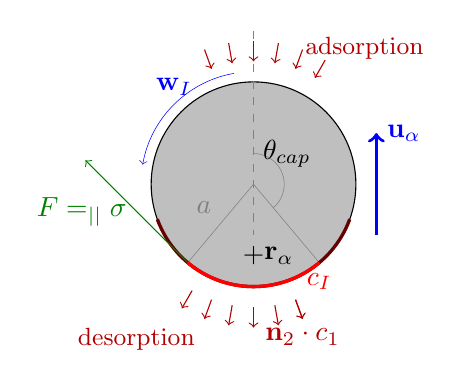
\begin{tikzpicture}[scale =1.3]
        \draw[fill=lightgray](0,0) circle (1);
        \draw[very thin,gray](230:1)--(0,0)node[midway,above left]{$a$}--(310:1);
        \draw[very thin,gray](0,0)++(310:0.3) arc (-50:90:0.3)node[right,black]{$\theta_\text{cap}$};
        \draw[very thin,blue,->](0,0)++(100:1.1) arc (100:170:1.1)node[midway,above]{$\textbf{w}_I$};
        \draw[very thick,red!40!black](0,0)++(200:1) arc (200:340:1);
        \draw[very thick,red](0,0)++(230:1) arc (230:310:1)node[below]{$c_I$};
        \draw[very thick,dashed](0,0)++(0,-0.7)node{$+$}node[right]{$\textbf{r}_\alpha$};
        \draw[very thick,blue,->](1.2,-0.5)--++(0,1)node[right]{$\textbf{u}_\alpha$};
        \draw[dashed,gray](0,1.5)--++(0,-2);
        \draw[red,->,green!50!black](230:1)--++(-1,1)node[midway,left]{$F = \grad_{||} \sigma$};
        \foreach \t in {110,100,90,80,60}{
            \draw[red!70!black, ->](\t:1.4)--++(\t:-0.2);
            \draw[red!70!black, ->](\t:-1.2)--++(\t:-0.2);
        }
        \draw[red!70!black, ->](70:1.4)--++(70:-0.2)node[above right]{\small adsorption};
        \draw[red!70!black, ->](70:-1.2)--++(70:-0.2)node[below left]{\small desorption};
        \draw[red!70!black, ->](110:-1.2)--++(110:-0.2)node[below]{$\textbf{n}_2 \cdot \grad c_1$};
    \end{tikzpicture}
    \hspace{2em}
    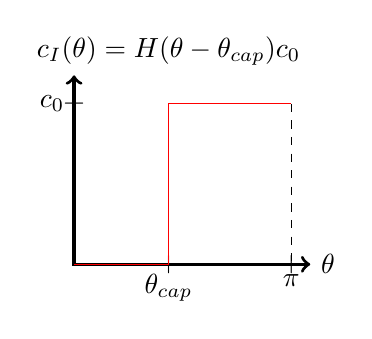
\begin{tikzpicture}[scale =1.2]
        \draw[very thick,<->](0,2)--(0,0)--(2.5,0)node[right]{$\theta$};
        \draw(1,0)node{$+$}node[below]{$\theta_{cap}$};
        \draw(1,2)node[above]{$c_I(\theta) = H(\theta- \theta_{cap}) c_0$};
        \draw[very thin,dashed](2.3,1.7)--(2.3,0);
        \draw[thin,red](0,0)--++(1,0)--++(0,1.7)--++(1.3,0);
        \draw(2.3,0)node{$+$}node[below]{$\pi$};
        \draw(0,1.7)node{$+$}node[left]{$c_0$};
    \end{tikzpicture}
    \caption{ (left) Scheme of the stagnant-cap regime of a rising contaminated bubble in a quiescent liquid. 
    (right) Hypothetical profile of the surface concentration $c_I$ in terms of the azimuthal coordinate $\theta$. }
    \label{fig:contaminated_bubbles}
\end{figure}


To derive the microscopic scale conservation equation of $c_I$ and $c_1$ we set $f_1 = c_1$ and $f_I = c_I$ in \ref{eq:dt_f_k} and \ref{eq:dt_f_I}, respectively.
Additionally, we assume that the  diffusive flux follow a Fick's law model, i.e.  $\mathbf{\Phi}_1 = D\grad c_1$ and $\mathbf{\Phi}_I = D_I\gradI c_I$,
where the constant,  $D$ and $D_I$ are the volumetric and surface diffusion coefficient, respectively.
Note that this diffusive model remains true under the assumption of dilute species concentration in both the liquid and at the interface.
\tb{The diffusive terms change in function of the regime : dilute concentration / saturated concentration, in which case $D\grad c_1 = f(c_I)$, it is worth going into that mush details ? no.}
Moreoverer, We do not consider chemical reaction or any other source term, i.e. $\textbf{S}_k = 0$ and $\textbf{S}_I=0$. 
Then, by injecting these terms in \ref{eq:dt_f_k} and \ref{eq:dt_f_I} we obtain these conservation equations : 
\begin{align}
    \pddt c_1
    + \div (\textbf{u}_1 c_1)
    &= \div (D \grad c_1)
    \;\;\; \text{in} \;\;\; \Omega_1,\\
    \pddt c_I
    + \divI (\textbf{u}_I c_I)
    &= \divI (D_I \gradI c_I)
    - (D \grad c_1)\cdot \textbf{n}_2
    \;\;\; \text{on} \;\;\; \Sigma,
    \label{eq:dt_c_I}
\end{align}
In agreement with \citet{pesci2018computational,manikantan2020surfactant}.
We recognize that the last term of \ref{eq:dt_c_I}, namely $D(\grad c_1 ) \cdot \textbf{n}_2$, turns out to be the \textit{Kinetically controlled sorption} boundary condition \citet{pesci2018computational,manikantan2020surfactant} which arise naturally in our model.
Specifically, it represents the adsorption and desorption flux between the bulk and the surface, as represented in \ref{fig:contaminated_bubbles}.
% For clarity remark that for exemple Equation (3.9) of \citet{manikantan2020surfactant} corresponds to the \textit{two-fluid} formulation of \ref{eq:dt_c_I} with a Fick's law model. 
Note that this exchange term is reduced to a contribution from the continuous phase since we assume no surfactant into the dispersed phase. 
Now that we clearly derived the microscale equation in both phases, we can easily derive the averaged equations of conservation using the hybrid model presented \ref{sec:averaged_eq}.

For a better understanding of the following equations, we now describe the steady-state kinetics that can be reached for an isolated bubble in a contaminated flow, as illustrated on \ref{fig:contaminated_bubbles}.
This will serve as a reference for the subsequent discussion.
We first assume that the transport of surfactants on the surface, represented  by the term  $\textbf{w}_I c_I$, is much greater than the other diffusive processes, such as $D\grad c_1$ and $D_I\gradI c_I$ as well as the adsorption-desorption effects. 
In this regime, the concentration of surfactant that enters from the forward-surface, due to adsorption, is advected almost instantaneously to the downward region of the particle where some of it evaporates due to desorption. 
This form an accumulation of surfactant on the downward region of the particle's surface.
At a certain point of equilibrium, the adsorption and desorption flux balance each other, leading to the steady-state kinetic of $c_I$, and the stagnant cap is stabilized to a concentration $c_0$. 
In this situation, we can consider that $c_I$ follows a constant sharp distribution along the azimuthal coordinate of the particle's surface.
Specifically, we model $c_I(\theta) = H(\theta - \theta_{cap}) c_0$ where $H$ is the Heaviside function and $\theta_{cap}$ is the angle at which the stagnant cap is formed, see \ref{fig:contaminated_bubbles}.
This assumption might seem unrealistic, nevertheless in the steady-state regime, it is approximately consistent with the observations \citep{kentheswaran2022direct}.
% In these condition the physical meaning of the first moment, $\textbf{r}_\alpha$, becomes clearer. 
From the expression of $c_I$ we deduce : $C_\alpha = \frac{c_0}{2}(1+\cos\theta_{cap})$ and $\textbf{r}_\alpha = \frac{a}{2} (\cos\theta_{cap} -1)\textbf{e}$ where $\textbf{e}$ is the unit vector in the direction of the relative velocity between the particle and the continuous phase velocity.
Thus, the knowing $\textbf{r}_\alpha$ can leads use to $\theta_{cap}$. 
This is crucial information, since the drag forces term and mass transfer closure terms are usually derived in terms of $\theta_{cap}$, such as in the following studies : \citet{sadhal1983stokes} and \citet{kentheswaran2022direct}. 

Now that the problem has been properly formulated, we can begin the derivation of the averaged equations.
The phase-averaged conservation equation for the mean concentration of surfactant in the bulk $\oneavg{c}$, is derived using \ref{eq:avg_dt_chi_f}.
It reads as,
\begin{equation}
    \pddt (\phi_1 \oneavg{c})
    + \div (\phi_1 \oneavg{c} \oneavg{\textbf{u}_1})
    = D \grad^2 (\phi_1\oneavg{c})
    - \pnavg{j_\alpha}
    +  \div \mathbf{\Sigma}_c,
    \label{eq:hybrid_avg_dt_c_1}
\end{equation}
where $j_\alpha$ is the exchange term with the dispersed phase given by,
\begin{equation*}
    j_\alpha
    =\int_{\Sigma_\alpha}
    (D\grad c_1 )
\cdot \textbf{n}_2d\Sigma,
\end{equation*}
which corresponds to the resultant of the surfactant exchange including adsorption and desorption flux.  
In the steady-state regime, when the adsorption flux balance the desorption flux,  the surfactant on the surface of the bubble can be considered as globally insoluble since $j_\alpha=0$ even through $D(\grad c_1 ) \cdot \textbf{n}_2$ may not be locally zero. 
This \textit{globally insoluble} assumption has been used in numerous studies to neglect the adsorption-desorption fluxes. 
The vector $\mathbf{\Sigma}_c$ in \ref{eq:hybrid_avg_dt_c_1}, has the following expression,
\begin{equation}
    \mathbf{\Sigma}_c
    =
     \pnavg{\textbf{J}_\alpha}
    - \pnavg{\frac{D}{a}\int_{\Sigma_\alpha}  c_1 \textbf{r} d\Sigma}
    - \phi_1\oneavg{c'_1\textbf{u}_1'},
    \label{eq:B_def}
\end{equation}
where the higher order terms have been neglected. 
The first term on the RHS of \ref{eq:B_def} corresponds to the first moment of the surfactant flux, namely $\textbf{J}_\alpha = \int_{\Sigma_\alpha} \textbf{r}
(D\grad c_1)\cdot \textbf{n}_2d\Sigma$.
It can be interpreted as the vector representing the mean direction and magnitude of the surfactant flux going in and out the surface of the droplets.
In the stagnant cap regime, this term is therefore non-zero since a mean flux is still present even through its resultant is null, i.e. $j_\alpha=0$.
In the reference frame of the particles, $\textbf{J}_\alpha$ account for the mean flux of species concentration induced by the presence of the particles, due to adsorption and desorption phenomena. 
The second term of \ref{eq:B_def} comes from the inclusion of $\phi_1$ inside the Laplacian operator in \ref{eq:hybrid_avg_dt_c_1}.
It is the first moment of $c_1$ over the droplets surface, thus it is the mean position of the continuous phase surfactant concentration over the droplet surface.
For a constant distribution $c_1$ at the bubbles interface, this vector would be zero. 
Finally, The last term of \ref{eq:B_def}, $\phi_1\oneavg{c'_1\textbf{u}_1'}$, represents the diffusive term due to the correlation of $c'_1$ with $\textbf{u}_1'$.
Overall, $\mathbf{\Sigma}_c$ is a balance between the first moment of the fluxes and the first moment of the bulk concentration, minus a contribution from the fluctuations.
Note that $\mathbf{\Sigma}_c$ appear under the divergence operator in \ref{eq:hybrid_avg_dt_c_1}, thus it will be relevant only in highly inhomogeneous cases. 
% At this stage of the research it is hard to predict the form of these closure terms. 
% Nevertheless, we know that the closure for $j_\alpha$ and $\mathbf{\Sigma}_c$ are function of the mean surface concentration $C_\alpha$ and its center of distribution $\textbf{r}_\alpha$.
% Indeed, the exchange term $\grad c_1$ which is function of the local concentration $c_I$ at surfactant saturation \citep{manikantan2020surfactant}. 
% Thus, an equation for $C_\alpha$ and a moment equation for $\textbf{r}_\alpha$ are needed. 

Regarding the equations dispersed phase, we start by the transport equation of the mean surface surfactant concentration $C_\alpha$.
From \ref{eq:avg_dt_dq_alpha_tot} the averaged conservation equation of $C_\alpha$ is straightforward to obtain and reads as,
\begin{equation}
    \pddt (\pnavg{C_\alpha})
    + \div (\pnavg{\textbf{u}_\alpha} \pnnavg{C_\alpha})
    =
    \frac{\pnavg{j_\alpha}}{s_\alpha}
    - \div (\pnavg{\textbf{u}_\alpha' C'_\alpha}).
    \label{eq:avg_dt_dC_alpha}
\end{equation}
As shown by this equation, the evolution of the mean concentration of surfactant on the particles' surface is driven by the exchange term $j_\alpha$ and the fluctuation term $\pnnavg{\textbf{u}_\alpha' C_\alpha'}$. 
The latter term is the covariance between the velocity of the particles and their mean surfactant concentration. 
It is known that the rising velocity of a bubble is greatly correlated with its mean surfactant concentration \citet{kentheswaran2022direct} thus it might be of a certain importance. 
Again, this term is under the divergence operator it will be therefore important only in non-homogeneous cases. 
Anyhow, this term must be further investigated.

We now derive an equation for the mean position of the surfactant, $\pnnavg{\textbf{r}_\alpha}$.
This is done by deriving the equation of the first moment, $s_\alpha C_\alpha \textbf{r}_\alpha$ using \ref{eq:dt_Q_alpha_tot}. 
Then, we reformulate the equation using  the relation, $\ddt (s_\alpha C_\alpha \textbf{r}_\alpha) = s_\alpha C_\alpha\ddt \textbf{r}_\alpha+ s_\alpha \textbf{r}_\alpha\ddt C_\alpha $ and  $\ddt C_\alpha = j_\alpha$. 
Finally,  we apply the average process which leads us to~:
\begin{multline}
    \pddt (\pnavg{\textbf{r}_\alpha})
    + \div (\pnavg{\textbf{u}_\alpha}\pnnavg{\textbf{r}_\alpha})
    =
    - \div (\pnavg{\textbf{u}'_\alpha\textbf{r}'_c})\\
    + \frac{n_p}{s_\alpha}\pnnavg{
        \frac{1}{C_\alpha}\left[
            \int_{\Sigma_\alpha} 
            \left[
                c_I \textbf{w}_I
                - D_I (\gradI c_I)
            \right] d\Sigma
            +\textbf{J}_\alpha
            - \textbf{r}_\alpha j_\alpha
        \right]
    }.
    \label{eq:avg_dt_dr_alpha_tot}
\end{multline}
The diffusive term $\pnavg{\textbf{u}'_\alpha\textbf{r}'_c}$ which represents the flux generated by the correlation between the mean surfactant distribution on the particles' surface and the velocity of the particles. 
Again, this term might be relevant since, as mentioned previously, the rising velocity is highly dependent on $\theta_{cap}$.
Then, the first term on the second line is the contribution of the averaged surface advection of $c_I$ along the particles' surface. 
The second term accounts for the diffusion of surfactants over the droplet surface, which acts against the formation of a sharp distribution of surfactants.
However, the contribution of this term is likely negligible based on the values of the diffusive surface coefficient, as discussed in \citet{valkovska2000determination}.
The third term of the second line, is the exchange term $\textbf{J}_\alpha$ which clearly impacts $\textbf{r}_\alpha$.
Indeed, this term accounts for the inward adsorption of concentration and downward desorption fluxes of surfactant, creating a significant disequilibrium. 
The last term, $\textbf{r}_\alpha j_\alpha$, is the contribution from the accumulation of species adsorption and desorption on the particle surface during the process driven by the three previous terms, i.e. adsorption, advection, diffusion and desorption. 
We may recognize that the latter fourth terms are being responsible for the equilibrium or not of the cap angle. 
Indeed, when all these terms are balanced, the system reaches a steady-state equilibrium for the surfactant distribution.
It is evident that in the closure of \ref{eq:avg_dt_dr_alpha_tot} one can include all properties linked to the physics of the bubbles' surface, which in turn creates a model for the surfactant distribution at first order. 

\tb{Dans cette partie il faut encore que je lise la bibliography qui existe peut etre sur ces dernière equaiton pour voir i le tout est bien coherent}

% \tb{Start : in the SSR the stagnat can is funciton of Re anfd Ma}
% Let assume that the timescale to reach the steady-state kinetic regime is much shorter than the variation of $\oneavg{c}$ seen by the particles. 
% In this situation the advection flux compensate the diffusive flux and adsorption-desorption source terms for all particles at all times.
% This equilibrium can be written :
% \begin{equation}
%     \int_{\Sigma_\alpha} 
%         c_I \textbf{w}_I
%         d\Sigma
%         - \int_{\Sigma_\alpha} 
%         D_I (\gradI c_I)
%          d\Sigma
%         +\textbf{J}_\alpha
%         = 0 
%         % - \textbf{r}_\alpha j_\alpha
%         \label{eq:steady_state_kinetic_regime}
% \end{equation}
% Nevertheless, due to a change of environment, $\oneavg{c}$ can change slowy inducing a non-zero $j_\alpha$, after what the particles reache instantaneously another steady-state kinetic regime. 
% In this situations the mean position of the surfactant is fully determined with the local concentration $\oneavg{c}$ or the local source $j_n$.
% Using the hypothesis \ref{eq:steady_state_kinetic_regime} in \ref{eq:avg_dt_dr_alpha_tot} gives the quasy steady conservation equaiton of $\textbf{r}_c$ with :
% \begin{equation}
%     \pddt (\pnavg{\textbf{r}_\alpha})
%     + \div (\pnavg{\textbf{u}_\alpha}\pnnavg{\textbf{r}_\alpha})
%     =
%     - \frac{n_p}{s_\alpha}\pnnavg{
%          \frac{\textbf{r}_\alpha j_\alpha}{C_\alpha}
%     }
%     - \div (\pnavg{\textbf{u}'_\alpha\textbf{r}'_c})
% \end{equation}
% where $\textbf{r}_\alpha$ is solely function on the local flux on the a the diffusive fluctuation term. 


As the objective of this study is not to provide a fully closed system, we will conclude the discussion on this point.
In short, this new system of equations can be used to determine the macroscopic variables $\pnnavg{C_\alpha}$ and $\pnnavg{\textbf{r}_\alpha}$, which are crucial for the closure of drag force and mass transfer in the macroscopic models.
Unfortunately, at the current state of the art, it is still challenging to derive exact closure terms for these equations, even in simplified regimes. 
However, we provided a clear methodology to derive a hybrid model tailored to the problem at hand, using the examples of surfactant transport and fiber suspension. 


% \section{Brouillion}
\subsection*{Fluid formulation meaningful exchange terms}


Using the generic formulation \ref{eq:hybrid_avg_dt_chif} and the local expression of the mass, momentum and total energy expression, i.e. : \ref{eq:dt_rho},\ref{eq:dt_rhou_1} and \ref{eq:dt_rhoE_1} we easily find the averaged form of these equations as, 

\begin{align}
    \pddt (\phi_1 \rho_1)  
    + \div (
        \phi_1 \rho_1\textbf{u}_1
    )
    &= 
    0\\
    \pddt (\phi_1 \rho_1\textbf{u}_1)  
    + \div (
        \phi_1 \rho_1\textbf{u}_1\textbf{u}_1
        + \bm{\sigma}_1^\text{eq}
    )
    &= 
    \phi_1 \rho_1 \textbf{g} 
    -  \avg{\delta_I \bm{\sigma}_1^0 \cdot \textbf{n}_2}\\
    \pddt (\phi_1\rho_1E_1)  
    + \div (
        \phi_1\rho_1E_1\textbf{u}_1
        + \bm{q}_1^\text{eq}
        + \textbf{u}_1 \cdot \bm{\sigma}_1^\text{eq}
        % - \textbf{u}_1^0 \cdot \bm{\sigma}_1^0 
        % + \textbf{q}_1^0
        )
    &= 
    \phi_1 \rho_1\textbf{u}_1 \cdot \textbf{g} 
    - \avg{\delta_I (\textbf{u}_1^0 \cdot \bm{\sigma}_1^0 - \textbf{q}_1^0)\cdot \textbf{n}_2}
\end{align} 
where we have defined, 
\begin{align*}
    &\bm{\sigma}_1^\text{eq}
    = \phi_1 (
        \rho_1\kavg{\textbf{u}_1'\textbf{u}_1'}
        - \bm{\sigma}_1%- n_p \textbf{M}_p
         )  
    &\textbf{q}_1^\text{eq}
    =\textbf{q}_1^\text{e} +\textbf{q}_1^\text{k}  \\
    &\textbf{q}_1^\text{e}
    = \phi_1\rho_1 \kavg{\textbf{u}_1' e_1'} 
    + \phi_1\textbf{q}_1 
    &\textbf{q}_1^\text{k}
    = \phi_1\rho_1 \kavg{\textbf{u}_1' k_1} 
    - \phi_1\kavg{\textbf{u}_1' \cdot \bm{\sigma}_1^0}
\end{align*}
Note that the phase averaged energy equation can be further decompose following, 
\begin{align*}
    E_1 = e_1 + k_1 + u_1^2/2
    \label{eq:E_def}
\end{align*}
where $K_1$ is the pseudo-turbulent kinetic energy defined such as, $\phi_1 k_1 = \avg{\chi_1 (u_1')^2/2}$. 
The Macroscopic kinetic energy equation can be obtain by taking the dot product with $\textbf{u}_1$. 
\begin{align}
    \pddt (\phi_1 \rho_1u_1^2/2)  
    + \div (
        \phi_1 \rho_1\textbf{u}_1u_1^2/2
        + \textbf{u}_1 \cdot \bm{\sigma}_1^\text{eq}
    )
    &= 
     \bm{\sigma}_1^\text{eq} : \grad \textbf{u}_1
    + \phi_1 \rho_1 \textbf{u}_1\cdot \textbf{g} 
    -  \textbf{u}_1\cdot \avg{\delta_I \bm{\sigma}_1^0 \cdot \textbf{n}_2}\\
    \pddt (\phi_1\rho_1k_1)  
    + \div (
        \phi_1\rho_1k_1\textbf{u}_1
        + \textbf{q}_1^\text{k} 
        )
    &= 
    - \avg{\chi_1\bm{\sigma}_1^0 : \grad \textbf{u}_1^0}
    - \bm{\sigma}_1^\text{eq} : \grad \textbf{u}_1
    - \avg{\delta_I \textbf{u}_1' \cdot \bm{\sigma}_1^0 \cdot \textbf{n}_2}\\
    \pddt (\phi_1\rho_1e_1)  
    + \div (
        \phi_1 \rho_1e_1\textbf{u}_1
        +
        \textbf{q}_1^\text{e} 
        )
    &= 
    \avg{\chi_1\bm{\sigma}_1^0 : \grad \textbf{u}_1^0}
    + \avg{\delta_I \textbf{q}_1^0 \cdot \textbf{n}_2} 
\end{align}


Let's decompose the exchange term $\avg{\delta_I \textbf{u}^0_1 \cdot \bm{\sigma}_1^0 \cdot \textbf{n}_2}$.
The first step is to make appear the drag force term 
\begin{align*}
    \avg{\delta_I \textbf{u}^0_1 \cdot \bm{\sigma}_1^0 \cdot \textbf{n}_2}
    = 
    \avg{\delta_I \textbf{u}^0_2 \cdot \bm{\sigma}_1^0 \cdot \textbf{n}_2}
    =
    \textbf{u}_p \cdot  \avg{\delta_I \bm{\sigma}_1^0 \cdot \textbf{n}_2}
    % + \avg{\delta_I (\textbf{u}_\alpha - \textbf{u}_p) \cdot \bm{\sigma}_1^0 \cdot \textbf{n}_2}
    + \avg{\delta_I (\textbf{u}^0_2 - \textbf{u}_p) \cdot \bm{\sigma}_1^0 \cdot \textbf{n}_2}
\end{align*}
Maybe it is not the good way. In fact let first do that : 
\begin{align*}
    \avg{\delta_I \textbf{u}^0_1 \cdot \bm{\sigma}_1^0 \cdot \textbf{n}_2}
    =
    \pavg{ \intS{\textbf{u}^0_2 \cdot \bm{\sigma}_1^0 \cdot \textbf{n}_2}}
    - \div\pavg{ \intS{\textbf{r}\textbf{u}^0_2 \cdot \bm{\sigma}_1^0 \cdot \textbf{n}_2}}
\end{align*}
The first term can then be written as, 
\begin{align*}
    \pavg{ \intS{\textbf{u}^0_2 \cdot \bm{\sigma}_1^0 \cdot \textbf{n}_2}}
    = 
    \textbf{u}_p \cdot \pavg{\intS{\bm{\sigma}_1^0 \cdot \textbf{n}_2}}
    + \pavg{ \textbf{u}_\alpha' \cdot \intS{  \bm{\sigma}_1^0 \cdot \textbf{n}_2}}
    + \pavg{ \intS{\textbf{w}_2^0 \cdot \bm{\sigma}_1^0 \cdot \textbf{n}_2}}
\end{align*}
\begin{align*}
    \pavg{ \intS{\textbf{r}\textbf{u}^0_2 \cdot \bm{\sigma}_1^0 \cdot \textbf{n}_2}}
    = 
    \textbf{u}_p \cdot \pavg{\intS{ \textbf{r}\bm{\sigma}_1^0 \cdot \textbf{n}_2}}
    + \pavg{ \textbf{u}_\alpha' \cdot \intS{ \textbf{r} \bm{\sigma}_1^0 \cdot \textbf{n}_2}}
    + \pavg{ \intS{\textbf{r}\textbf{w}_2^0 \cdot \bm{\sigma}_1^0 \cdot \textbf{n}_2}}
\end{align*}
Here we have a proper decomposition into surface work etc.. 


Using this formulation we can say that, 
\begin{align}
    \label{eq:dt_avg_rho}
    &\pddt (\phi_1 \rho_1)  
    + \div (
        \phi_1 \rho_1\textbf{u}_1
    )
    = 
    0\\
    \label{eq:dt_avg_rhou_1}
    &\pddt (\phi_1 \rho_1\textbf{u}_1)  
    + \div (
        \phi_1 \rho_1\textbf{u}_1\textbf{u}_1
        + \bm{\sigma}_1^\text{eq}
    )
    = 
    \phi_1 \rho_1 \textbf{g} 
    - \pavg{\intS{\bm{\sigma}_1^0 \cdot \textbf{n}_2}}
    +\div  \pavg{\intS{\textbf{r}\bm{\sigma}_1^0 \cdot \textbf{n}_2}}
    \\
    \label{eq:dt_avg_rhoE_1}
    &\pddt (\phi_1\rho_1E_1)  
    + \div (
        \phi_1\rho_1E_1\textbf{u}_1
        + \bm{q}_1^\text{eq}
        + \textbf{u}_1 \cdot \bm{\sigma}_1^\text{eq}
        % - \textbf{u}_1^0 \cdot \bm{\sigma}_1^0 
        % + \textbf{q}_1^0
        )
    = 
    \phi_1 \rho_1\textbf{u}_1 \cdot \textbf{g} \\
    &- \textbf{u}_p \cdot \pavg{\intS{\bm{\sigma}_1^0 \cdot \textbf{n}_2}}
    - \pavg{ \textbf{u}_\alpha' \cdot \intS{  \bm{\sigma}_1^0 \cdot \textbf{n}_2}}
    - \pavg{ \intS{\textbf{w}_2^0 \cdot \bm{\sigma}_1^0 \cdot \textbf{n}_2}}
    + \pavg{\intS{\textbf{q}_1\cdot \textbf{n}_2}}
    % &\div [    
        % \textbf{u}_p \cdot \pavg{\intS{ \textbf{r}\bm{\sigma}_1^0 \cdot \textbf{n}_2}}
    % + \pavg{ \textbf{u}_\alpha' \cdot \intS{ \textbf{r} \bm{\sigma}_1^0 \cdot \textbf{n}_2}}
    % + \pavg{ \intS{\textbf{r}\textbf{w}_2^0 \cdot \bm{\sigma}_1^0 \cdot \textbf{n}_2}}
    % - \pavg{ \intS{\textbf{r}  \textbf{q}_1^0 \cdot \textbf{n}_2}}
    % ]
\end{align} 
where we have defined, 
\begin{align*}
    &\bm{\sigma}_1^\text{eq}
    = \phi_1 (
        \rho_1\kavg{\textbf{u}_1'\textbf{u}_1'}
        -\bm{\sigma}_1%- n_p \textbf{M}_p
        )  
        - \pavg{\intS{\textbf{r}\bm{\sigma}_1^0 \cdot \textbf{n}_2}}\\
    &\textbf{q}_1^\text{eq}
    =\textbf{q}_1^\text{e} +\textbf{q}_1^\text{k}  \\
    &\textbf{q}_1^\text{e}
    = \phi_1\rho_1 \kavg{\textbf{u}_1' e_1'} 
    + \phi_1\textbf{q}_1 
    +\pavg{\intS{\textbf{r}\textbf{q}_1^0 \cdot \textbf{n}_2}} 
    \\
    &\textbf{q}_1^\text{k}
    = \phi_1\rho_1 \kavg{\textbf{u}_1' k_1} 
    - \phi_1\kavg{\textbf{u}_1' \cdot \bm{\sigma}_1^0}
    + (\textbf{u}_1 - \textbf{u}_p)\cdot
    \pavg{\intS{\textbf{r}\bm{\sigma}_1^0 \cdot \textbf{n}_2}}
    \\
    &+ \pavg{ \textbf{u}_\alpha' \cdot \intS{ \textbf{r} \bm{\sigma}_1^0 \cdot \textbf{n}_2}}
    + \pavg{ \intS{\textbf{r}\textbf{w}_2^0 \cdot \bm{\sigma}_1^0 \cdot \textbf{n}_2}}
\end{align*}
Let's re derive the Secondary equations, firstly the kinetic energy equaitons, 
\begin{align*}
    \pddt (\phi_1 \rho_1u_1^2/2)  
    + \div (
        \phi_1 \rho_1\textbf{u}_1u_1^2/2
        + \textbf{u}_1 \cdot \bm{\sigma}_1^\text{eq}
    )
    &= 
     \bm{\sigma}_1^\text{eq} : \grad \textbf{u}_1
    + \phi_1 \rho_1 \textbf{u}_1\cdot \textbf{g} 
    -  \textbf{u}_1\cdot 
        \pavg{\intS{\bm{\sigma}_1^0 \cdot \textbf{n}_2}} 
        % - \div 
        % \pavg{\intS{\textbf{r}\bm{\sigma}_1^0 \cdot \textbf{n}_2}} 
        \\
    \pddt (\phi_1\rho_1k_1)  
    + \div (
        \phi_1\rho_1k_1\textbf{u}_1
        + \textbf{q}_1^\text{k} 
        )
    &= 
    - \avg{\chi_1\bm{\sigma}_1^0 : \grad \textbf{u}_1^0}
    - \bm{\sigma}_1^\text{eq} : \grad \textbf{u}_1\\
    &+ (\textbf{u}_1 - \textbf{u}_p)
    \cdot \pavg{\intS{\bm{\sigma}_1^0 \cdot \textbf{n}_2}}\\
    &- \pavg{ \textbf{u}_\alpha' \cdot \intS{  \bm{\sigma}_1^0 \cdot \textbf{n}_2}}
    - \pavg{ \intS{\textbf{w}_2^0 \cdot \bm{\sigma}_1^0 \cdot \textbf{n}_2}} 
    \\
    \pddt (\phi_1\rho_1e_1)  
    + \div (
        \phi_1 \rho_1e_1\textbf{u}_1
        +
        \textbf{q}_1^\text{e} 
        )
    &= 
    \avg{\chi_1\bm{\sigma}_1^0 : \grad \textbf{u}_1^0}
    + \pavg{\intS{\textbf{q}_1^0 \cdot \textbf{n}_2}} 
\end{align*}
The second equality here, gives in a homogeneous medium, 
\begin{equation*}
    0 =
    - \avg{\chi_1\bm{\sigma}_1^0 : \grad \textbf{u}_1^0}
    % - \bm{\sigma}_1^\text{eq} : \grad \textbf{u}_1
    + (\textbf{u}_1 - \textbf{u}_p)
    \cdot \pavg{\intS{\bm{\sigma}_1^0 \cdot \textbf{n}_2}}
    - \pavg{ \textbf{u}_\alpha' \cdot \intS{  \bm{\sigma}_1^0 \cdot \textbf{n}_2}}
    - \pavg{ \intS{\textbf{w}_2^0 \cdot \bm{\sigma}_1^0 \cdot \textbf{n}_2}} 
\end{equation*}
\subsection*{Particle formulation meaningful exchange terms}

For the dispersed phase we initially have :
\begin{align*}
    \pddt \left(n_p m_p\right)
    + \div \left(n_pm_p\textbf{u}_p
    \right)
    = 
    0\\
    \pddt \left(n_p m_p \textbf{u}_p\right)
    + \div \left(n_p
    m_p \textbf{u}_p \textbf{u}_p 
    + \bm{\sigma}_p^\text{eq}
    \right)
    = 
    n_p v_p \rho_2 \textbf{g}
    + n_p (\bm{\sigma}_1^0 \cdot \textbf{n}_2)_p^\Sigma,\\
    \pddt(m_p n_pE_p^\text{tot})
    + \div(m_pn_p E_p^\text{tot} \textbf{u}_p 
    + \textbf{q}_p^\text{eq} 
    + \textbf{u}_p \cdot \bm{\sigma}_p^\text{eq})
    =  n_p v_p \rho_2 \textbf{u}_p\cdot  \textbf{g}\\
    % +  n_p ( \textbf{u}'_1 \cdot \bm{\sigma}_1^0 \cdot \textbf{n}_2)_p^\Sigma
    -  n_p (\textbf{q}_1^0 \cdot \textbf{n}_2)_p^\Sigma
    + \textbf{u}_p \cdot\pavg{\intS{\bm{\sigma}_1^0 \cdot \textbf{n}_2}}
    + \pavg{\intS{\textbf{u}_\alpha' \cdot\bm{\sigma}_1^0 \cdot \textbf{n}_2}}
    + \pavg{\intS{\textbf{w}_2^0 \cdot\bm{\sigma}_1^0 \cdot \textbf{n}_2}}
\end{align*}
where we have defined, 
\begin{align*}
    &\bm{\sigma}_p^\text{eq}
    =  m_p\pnavg{\textbf{u}_\alpha'\textbf{u}_\alpha'}
    &\textbf{q}_p^\text{eq}
    =\textbf{q}_p^\text{e} 
    +\textbf{q}_p^\text{k}  
    +\textbf{q}_p^\text{w}  
    \\
    &\textbf{q}_1^\text{e}
    = m_p \pnavg{\textbf{u}_\alpha' e_\alpha'} 
    &\textbf{q}_p^\text{k}
    = m_p \pnavg{\textbf{u}_\alpha' k_\alpha} 
    \\
    &\textbf{q}_p^\text{w}
    = 
    + \pnavg{\textbf{u}_\alpha'(\rho_2 (w^0_2)^2/2 )'_\Omega}
    + \gamma \pnavg{\textbf{u}_\alpha' s_\alpha'}
\end{align*}
and, 
The exchange term of the energy equation can be rewritten as, 
\begin{equation*}
    \pavg{\intS{\textbf{u}_1^0\cdot\bm{\sigma}_1^0 \cdot \textbf{n}_2}}
    = 
    \textbf{u}_p \cdot\pavg{\intS{\bm{\sigma}_1^0 \cdot \textbf{n}_2}}
    + \pavg{\intS{\textbf{u}_\alpha' \cdot\bm{\sigma}_1^0 \cdot \textbf{n}_2}}
    + \pavg{\intS{\textbf{w}_2^0 \cdot\bm{\sigma}_1^0 \cdot \textbf{n}_2}}
\end{equation*}
Also, 
\begin{align*}
    &\pddt \left(n_p m_p u_p^2/ 2\right)
    + \div \left(n_p
    m_p u_p^2/ 2 \textbf{u}_p 
    + \textbf{u}_p \cdot \bm{\sigma}_p^\text{eq}
    \right)
    = 
    + \bm{\sigma}_p^\text{eq}  :\grad \textbf{u}_p
    +  n_p v_p \textbf{u}_p \cdot 
    \rho_2 \textbf{g}
    + n_p \textbf{u}_p \cdot (\bm{\sigma}_1^0 \cdot \textbf{n}_2)^\Sigma_p,\\
    &\pddt \left(n_p m_p (u_\alpha^2)_p/ 2\right)
    + \div \left(n_p
    m_p (u_\alpha^2)_p/ 2 \textbf{u}_p 
    + \textbf{q}^k_p
    + \textbf{u}_p \cdot \bm{\sigma}_p^\text{eq}
    \right)
    = 
    n_p m_p \textbf{u}_p \cdot
    \textbf{g}
    + \textbf{u}_p\cdot\pavg{\intS{\bm{\sigma}_1^0 \cdot \textbf{n}_2}}\\
    &+ \pavg{\textbf{u}_\alpha'\cdot\intS{\bm{\sigma}_1^0 \cdot \textbf{n}_2}}
    \\
    &\pddt \left(n_p W_p\right)
    + \div 
    (n_p W_p
    \textbf{u}_p 
    +  \textbf{q}_p^\text{w}
    )
    = 
    - n_p (\bm{\sigma}_2^0 : \grad\textbf{u}_2^0)^\Omega_p
    + n_p (\textbf{w}_2^0 \cdot \bm{\sigma}_1^0 \cdot  \textbf{n}_2)^\Sigma_p
    \\
    &\pddt \left(n_p m_p e_p\right)
    + \div \left(n_p
    m_p e_p \textbf{u}_p 
    +  \textbf{q}_p^\text{e}
    \right)
    = 
    + n_p (\bm{\sigma}_2^0 : \grad\textbf{u}_2^0)^\Omega_p
    - n_p (\textbf{q}_1^0\cdot \textbf{n}_2)^\Sigma_p\\
\end{align*}
The equaiton for $k_p$ reads, 
\begin{equation*}
    \pddt \left(n_p m_p k_p\right)
    + \div \left(n_p
    m_p k_p \textbf{u}_p 
    + \textbf{q}^k_p
    % + \textbf{u}_p \cdot \bm{\sigma}_p^\text{eq}
    \right)
    = 
    - \bm{\sigma}_p^\text{eq}  :\grad \textbf{u}_p
    + \pavg{\textbf{u}_\alpha'\cdot\intS{\bm{\sigma}_1^0 \cdot \textbf{n}_2}}
\end{equation*}
In agreement with kinetic theory without source term. 


Under this form the NRJ cascade takes the form
\begin{center}
    \tikzstyle{quadri}=[rectangle,draw]
    \begin{tikzpicture}
        \node[quadri] (u2) at (0,0){$(u_p)^2 / 2$};
        \node[quadri] (kp) at (4,0){$(k_p)$};
        \node[quadri] (Wp) at (8,0){$(W_p)$};
        \node[quadri] (ep) at (12,0){$(e_p)$};
        \node[quadri] (u12) at (2,-3){$\frac{\rho_1}{2}(u_1)^2$};
        \node[quadri] (k1) at (6,-3){$k_1$};
        \node[quadri] (e1) at (10,-3){$e_1$};
        \draw[->] (u2)--(kp)node[midway,above]{\footnotesize $\bm{\sigma}^\text{eq}:\grad \textbf{u}_1$};
        \draw[<->] (u2)--(u12) node[midway,left]{\footnotesize $\textbf{f}_{p} $};
        % \draw[<->,text width=2cm] (kp)--(u12) node[midway,left]{\footnotesize $+  n_p v_p \textbf{u}_p \cdot 
        % (\rho_2 \textbf{g} - \grad p_1)
        % + n_p \textbf{u}_p \cdot \textbf{f}_{pm} - \textbf{F}_\text{pfp}$};
        \draw[<->] (k1)--(u12) node[midway,below]{\footnotesize $\bm{\sigma}^\text{eq}_1:\grad \textbf{u}_1$, $\textbf{f}_p$};
        \draw[<->] (k1)--(e1) node[midway,below]{\footnotesize $\textbf{d}_1$};
        \draw[<->,sloped] (k1)--(kp) node[midway,below]{\footnotesize $\pavg{\textbf{f}_\alpha\cdot \textbf{u}_\alpha'}$};
        \draw[<->] (k1)--(u2) node[midway,below]{\footnotesize $\textbf{f}_p$};
        \draw[<->,sloped] (k1)--(Wp) node[midway,below]{\footnotesize $\pavg{\intS{\textbf{w}_2^0\cdot \textbf{f}_1^0}}$};
        % \draw[->] (kp)--(Wp)node[midway,above]{$(\textbf{u}_\alpha' \cdot \textbf{f}_\alpha')_p$};
        \draw[->] (Wp)--(ep)node[midway,above]{$\textbf{d}_p$};
        \draw[->] (e1)--(ep)node[midway,above]{$\textbf{q}_p$};
    \end{tikzpicture}
\end{center}

Thus, from this graph it is clear that the only way to makes the link between $k_p$ and the NRJ dissipation is through the addition of $k_p$ and $W_p$. Which gives, 
\begin{multline*}
    \pddt \left(n_p (W_p+m_p k_p)\right)
    + \div 
    (n_p (W_p+m_p k_p)
    \textbf{u}_p 
    +  \textbf{q}_p^\text{w}
    +  \textbf{q}_p^\text{k}
    )\\
    = 
    - n_p (\bm{\sigma}_2^0 : \grad\textbf{u}_2^0)^\Omega_p
    + n_p (\textbf{w}_2^0 \cdot \bm{\sigma}_1^0 \cdot  \textbf{n}_2)^\Sigma_p
    - \bm{\sigma}_p^\text{eq}  :\grad \textbf{u}_p
    + \pavg{\textbf{u}_\alpha'\cdot\intS{\bm{\sigma}_1^0 \cdot \textbf{n}_2}}
\end{multline*}
Here we recover the transfer terms of with the higher scales and the lower scales plus the ones of the fluid continuous phase...
In kinetic theory we consider non-slipping spherical particles such that the internal motion are constant, and non rotation is present.
In this situation it yields 
\begin{equation}
    \pddt \left(n_p m_p k_p\right)
    + \div 
    (n_p m_p k_p
    \textbf{u}_p 
    % +  \textbf{q}_p^\text{w}
    +  \textbf{q}_p^\text{k}
    )
    = 
    - n_p (\bm{\sigma}_2^0 : \grad\textbf{u}_2^0)^\Omega_p
    + n_p (\textbf{w}_2^0 \cdot \bm{\sigma}_1^0 \cdot  \textbf{n}_2)^\Sigma_p
    - \bm{\sigma}_p^\text{eq}  :\grad \textbf{u}_p
    + \pavg{\textbf{u}_\alpha'\cdot\intS{\bm{\sigma}_1^0 \cdot \textbf{n}_2}}
\end{equation}
Indeed, we still consider deformation inside the particles since a source term of dissipation is constant. 



\subsection{Inclusion of long range interactions}
\subsubsection*{Fluid phase}

Using this formulation we can say that, 
\begin{align}
    \label{eq:dt_avg_rho}
    &\pddt (\phi_1 \rho_1)  
    + \div (
        \phi_1 \rho_1\textbf{u}_1
    )
    = 
    0\\
    \label{eq:dt_avg_rhou_1}
    &\pddt (\phi_1 \rho_1\textbf{u}_1)  
    + \div (
        \phi_1 \rho_1\textbf{u}_1\textbf{u}_1
        + \bm{\sigma}_1^\text{eq}
    )
    = 
    \phi_1 \rho_1 \textbf{g} 
    % +  \pavg{\intS{\bm{\sigma}_1^0 \cdot \textbf{n}_2}}
    - n_p (\textbf{f}_\text{pm} + v_p \grad p_1)
    % +\div  \pavg{\intS{\textbf{r}\bm{\sigma}_1^0 \cdot \textbf{n}_2}}
    \\
    \label{eq:dt_avg_rhoE_1}
    &\pddt (\phi_1\rho_1E_1)  
    + \div (
        \phi_1\rho_1E_1\textbf{u}_1
        + \bm{q}_1^\text{eq}
        + \textbf{u}_1 \cdot \bm{\sigma}_1^\text{eq}
        % - \textbf{u}_1^0 \cdot \bm{\sigma}_1^0 
        % + \textbf{q}_1^0
        )
    = 
    \phi_1 \rho_1\textbf{u}_1 \cdot \textbf{g} 
    +n_p\textbf{F}_\text{pfp}:\grad \textbf{u}_p\\
    &
    - n_p \textbf{u}_p \cdot (\textbf{f}_\text{pm} + v_p \grad p_1)
    % \pavg{\intS{\bm{\sigma}_1^0 \cdot \textbf{n}_2}}
    - \pavg{ \textbf{u}_\alpha' \cdot \intS{  \bm{\sigma}_1^0 \cdot \textbf{n}_2}}
    - \pavg{ \intS{\textbf{w}_2^0 \cdot \bm{\sigma}_1^0 \cdot \textbf{n}_2}}
    + \pavg{\intS{\textbf{q}_1\cdot \textbf{n}_2}}
    % &\div [    
        % \textbf{u}_p \cdot \pavg{\intS{ \textbf{r}\bm{\sigma}_1^0 \cdot \textbf{n}_2}}
    % + \pavg{ \textbf{u}_\alpha' \cdot \intS{ \textbf{r} \bm{\sigma}_1^0 \cdot \textbf{n}_2}}
    % + \pavg{ \intS{\textbf{r}\textbf{w}_2^0 \cdot \bm{\sigma}_1^0 \cdot \textbf{n}_2}}
    % - \pavg{ \intS{\textbf{r}  \textbf{q}_1^0 \cdot \textbf{n}_2}}
    % ]
\end{align} 
where we have defined, 
\begin{align*}
    &\bm{\sigma}_1^\text{eq}
    = \phi_1 (
        \rho_1\kavg{\textbf{u}_1'\textbf{u}_1'}
        -\bm{\sigma}_1%- n_p \textbf{M}_p
        )  
        - \pavg{\intS{\textbf{r}\bm{\sigma}_1^0 \cdot \textbf{n}_2}}
        + \textbf{F}_\text{pfp}\\
    &\textbf{q}_1^\text{eq}
    =\textbf{q}_1^\text{e} +\textbf{q}_1^\text{k}  \\
    &\textbf{q}_1^\text{e}
    = \phi_1\rho_1 \kavg{\textbf{u}_1' e_1'} 
    + \phi_1\textbf{q}_1 
    +\pavg{\intS{\textbf{r}\textbf{q}_1^0 \cdot \textbf{n}_2}} 
    \\
    &\textbf{q}_1^\text{k}
    = \phi_1\rho_1 \kavg{\textbf{u}_1' k_1} 
    - \phi_1\kavg{\textbf{u}_1' \cdot \bm{\sigma}_1^0}
    + (\textbf{u}_1 - \textbf{u}_p)\cdot[
    \pavg{\intS{\textbf{r}\bm{\sigma}_1^0 \cdot \textbf{n}_2}}
     - n_p \textbf{F}_\text{pfp}]
    \\
    &+ \pavg{ \textbf{u}_\alpha' \cdot \intS{ \textbf{r} \bm{\sigma}_1^0 \cdot \textbf{n}_2}}
    + \pavg{ \intS{\textbf{r}\textbf{w}_2^0 \cdot \bm{\sigma}_1^0 \cdot \textbf{n}_2}}
\end{align*}
Let's re derive the Secondary equations, firstly the kinetic energy equaitons, 
\begin{align*}
    \pddt (\phi_1 \rho_1u_1^2/2)  
    + \div (
        \phi_1 \rho_1\textbf{u}_1u_1^2/2
        + \textbf{u}_1 \cdot \bm{\sigma}_1^\text{eq}
    )
    &= 
     \bm{\sigma}_1^\text{eq} : \grad \textbf{u}_1
    + \phi_1 \rho_1 \textbf{u}_1\cdot \textbf{g} 
    -  n_p \textbf{u}_1\cdot 
    (\textbf{f}_\text{pm} + v_1\grad p_1)
        % \pavg{\intS{\bm{\sigma}_1^0 \cdot \textbf{n}_2}} 
        % - \div 
        % \pavg{\intS{\textbf{r}\bm{\sigma}_1^0 \cdot \textbf{n}_2}} 
        \\
    \pddt (\phi_1\rho_1k_1)  
    + \div (
        \phi_1\rho_1k_1\textbf{u}_1
        + \textbf{q}_1^\text{k} 
        )
    &= 
    - \avg{\chi_1\bm{\sigma}_1^0 : \grad \textbf{u}_1^0}
    - \bm{\sigma}_1^\text{eq} : \grad \textbf{u}_1
    + n_p \textbf{F}_\text{pfp} : \grad \textbf{u}_p
    \\
    &+ n_p (\textbf{u}_1 - \textbf{u}_p)
    \cdot (\textbf{f}_\text{pm} - v_p \grad p_1)\\
    &- \pavg{ \textbf{u}_\alpha' \cdot \intS{  \bm{\sigma}_1^0 \cdot \textbf{n}_2}}
    - \pavg{ \intS{\textbf{w}_2^0 \cdot \bm{\sigma}_1^0 \cdot \textbf{n}_2}} 
    \\
    \pddt (\phi_1\rho_1e_1)  
    + \div (
        \phi_1 \rho_1e_1\textbf{u}_1
        +
        \textbf{q}_1^\text{e} 
        )
    &= 
    \avg{\chi_1\bm{\sigma}_1^0 : \grad \textbf{u}_1^0}
    + \pavg{\intS{\textbf{q}_1^0 \cdot \textbf{n}_2}} 
\end{align*}
The homogeneous equilibrium stays the same. 
\subsection*{Particle phase with pfp and dumped pressure}
On the particle phase


For the dispersed phase we initially have :
\begin{align*}
    \pddt \left(n_p m_p\right)
    + \div \left(n_pm_p\textbf{u}_p
    \right)
    = 
    0\\
    \pddt \left(n_p m_p \textbf{u}_p\right)
    + \div \left(n_p
    m_p \textbf{u}_p \textbf{u}_p 
    + \bm{\sigma}_p^\text{eq}
    \right)
    = 
    n_p v_p \rho_2 \textbf{g}
    + n_p (\textbf{f}_\text{pm} + v_p \grad p_1),
    \\
    \pddt(m_p n_pE_p^\text{tot})
    + \div(m_pn_p E_p^\text{tot} \textbf{u}_p 
    + \textbf{q}_p^\text{eq} 
    + \textbf{u}_p \cdot \bm{\sigma}_p^\text{eq})
    =  n_p v_p \rho_2 \textbf{u}_p\cdot  \textbf{g}
    % +  n_p ( \textbf{u}'_1 \cdot \bm{\sigma}_1^0 \cdot \textbf{n}_2)_p^\Sigma
    -  n_p (\textbf{q}_1^0 \cdot \textbf{n}_2)_p^\Sigma\\
    - n_p \textbf{F}_\text{pfp} : \grad \textbf{u}_p
    + \textbf{u}_p \cdot (\textbf{f}_\text{pm} + v_p\grad p_1)
    + \pavg{\intS{\textbf{u}_\alpha' \cdot\bm{\sigma}_1^0 \cdot \textbf{n}_2}}
    + \pavg{\intS{\textbf{w}_2^0 \cdot\bm{\sigma}_1^0 \cdot \textbf{n}_2}}
\end{align*}
where we have defined, 
\begin{align*}
    &\bm{\sigma}_p^\text{eq}
    =  m_p\pnavg{\textbf{u}_\alpha'\textbf{u}_\alpha'}
    - n_p \textbf{F}_\text{pfp}
    &\textbf{q}_p^\text{eq}
    =\textbf{q}_p^\text{e} 
    +\textbf{q}_p^\text{k}  
    +\textbf{q}_p^\text{w}  
    \\
    &\textbf{q}_1^\text{e}
    = m_p \pnavg{\textbf{u}_\alpha' e_\alpha'} 
    &\textbf{q}_p^\text{k}
    = m_p \pnavg{\textbf{u}_\alpha' k_\alpha} 
    \\
    &\textbf{q}_p^\text{w}
    = 
    + \pnavg{\textbf{u}_\alpha'(\rho_2 (w^0_2)^2/2 )'_\Omega}
    + \gamma \pnavg{\textbf{u}_\alpha' s_\alpha'}
\end{align*}
Also, 
\begin{align*}
    &\pddt \left(n_p m_p u_p^2/ 2\right)
    + \div \left(n_p
    m_p u_p^2/ 2 \textbf{u}_p 
    + \textbf{u}_p \cdot \bm{\sigma}_p^\text{eq}
    \right)
    = 
    + \bm{\sigma}_p^\text{eq}  :\grad \textbf{u}_p
    +  n_p v_p \textbf{u}_p \cdot 
    \rho_2 \textbf{g}
    + n_p \textbf{u}_p \cdot (\textbf{f}_\text{pm} + v_p \grad p_1),\\
    &\pddt \left(n_p m_p (u_\alpha^2)_p/ 2\right)
    + \div \left(n_p
    m_p (u_\alpha^2)_p/ 2 \textbf{u}_p 
    + \textbf{q}^k_p
    + \textbf{u}_p \cdot \bm{\sigma}_p^\text{eq}
    \right)
    = 
    n_p m_p \textbf{u}_p \cdot
    \textbf{g}
    + \textbf{u}_p\cdot(\textbf{f}_\text{pm} + v_p \grad p_1)\\
    &- n_p \textbf{F}_\text{pfp} : \grad \textbf{u}_p
    + \pavg{\textbf{u}_\alpha'\cdot\intS{\bm{\sigma}_1^0 \cdot \textbf{n}_2}}
    \\
    &\pddt \left(n_p W_p\right)
    + \div 
    (n_p W_p
    \textbf{u}_p 
    +  \textbf{q}_p^\text{w}
    )
    = 
    - n_p (\bm{\sigma}_2^0 : \grad\textbf{u}_2^0)^\Omega_p
    + n_p (\textbf{w}_2^0 \cdot \bm{\sigma}_1^0 \cdot  \textbf{n}_2)^\Sigma_p
    \\
    &\pddt \left(n_p m_p e_p\right)
    + \div \left(n_p
    m_p e_p \textbf{u}_p 
    +  \textbf{q}_p^\text{e}
    \right)
    = 
    + n_p (\bm{\sigma}_2^0 : \grad\textbf{u}_2^0)^\Omega_p
    - n_p (\textbf{q}_1^0\cdot \textbf{n}_2)^\Sigma_p\\
\end{align*}
The equaiton for $k_p$ reads, 
\begin{equation*}
    \pddt \left(n_p m_p k_p\right)
    + \div \left(n_p
    m_p k_p \textbf{u}_p 
    + \textbf{q}^k_p
    % + \textbf{u}_p \cdot \bm{\sigma}_p^\text{eq}
    \right)
    = 
    - \pavg{\textbf{u}_\alpha'\textbf{u}_\alpha'} :\grad \textbf{u}_p
    + \pavg{\textbf{u}_\alpha'\cdot\intS{\bm{\sigma}_1^0 \cdot \textbf{n}_2}}
\end{equation*}
In agreement with kinetic theory without source term. 


Under this form the NRJ cascade takes the form
\begin{center}
    \tikzstyle{quadri}=[rectangle,draw]
    \begin{tikzpicture}
        \node[quadri] (u2) at (0,0){$(u_p)^2 / 2$};
        \node[quadri] (kp) at (4,0){$(k_p)$};
        \node[quadri] (Wp) at (8,0){$(W_p)$};
        \node[quadri] (ep) at (12,0){$(e_p)$};
        \node[quadri] (u12) at (2,-3){$\frac{\rho_1}{2}(u_1)^2$};
        \node[quadri] (k1) at (6,-3){$k_1$};
        \node[quadri] (e1) at (10,-3){$e_1$};
        \draw[->] (u2)--(kp)node[midway,above]{\footnotesize $\bm{\sigma}^\text{eq}:\grad \textbf{u}_1$};
        \draw[<->] (u2)--(u12) node[midway,left]{\footnotesize $\textbf{f}_{p} $};
        % \draw[<->,text width=2cm] (kp)--(u12) node[midway,left]{\footnotesize $+  n_p v_p \textbf{u}_p \cdot 
        % (\rho_2 \textbf{g} - \grad p_1)
        % + n_p \textbf{u}_p \cdot \textbf{f}_{pm} - \textbf{F}_\text{pfp}$};
        \draw[<->] (k1)--(u12) node[midway,below]{\footnotesize $\bm{\sigma}^\text{eq}_1:\grad \textbf{u}_1$, $\textbf{f}_p$};
        \draw[<->] (k1)--(e1) node[midway,below]{\footnotesize $\textbf{d}_1$};
        \draw[<->,sloped] (k1)--(kp) node[midway,below]{\footnotesize $\pavg{\textbf{f}_\alpha\cdot \textbf{u}_\alpha'}$};
        \draw[<->] (k1)--(u2) node[midway,below]{\footnotesize $\textbf{f}_p$};
        \draw[<->,sloped] (k1)--(Wp) node[midway,below]{\footnotesize $\pavg{\intS{\textbf{w}_2^0\cdot \textbf{f}_1^0}}$};
        % \draw[->] (kp)--(Wp)node[midway,above]{$(\textbf{u}_\alpha' \cdot \textbf{f}_\alpha')_p$};
        \draw[->] (Wp)--(ep)node[midway,above]{$\textbf{d}_p$};
        \draw[->] (e1)--(ep)node[midway,above]{$\textbf{q}_p$};
    \end{tikzpicture}
\end{center}

Thus, from this graph it is clear that the only way to makes the link between $k_p$ and the NRJ dissipation is through the addition of $k_p$ and $W_p$. Which gives, 
\begin{multline*}
    \pddt \left(n_p (W_p+m_p k_p)\right)
    + \div 
    (n_p (W_p+m_p k_p)
    \textbf{u}_p 
    +  \textbf{q}_p^\text{w}
    +  \textbf{q}_p^\text{k}
    )\\
    = 
    - n_p (\bm{\sigma}_2^0 : \grad\textbf{u}_2^0)^\Omega_p
    + n_p (\textbf{w}_2^0 \cdot \bm{\sigma}_1^0 \cdot  \textbf{n}_2)^\Sigma_p
    - \bm{\sigma}_p^\text{eq}  :\grad \textbf{u}_p
    + \pavg{\textbf{u}_\alpha'\cdot\intS{\bm{\sigma}_1^0 \cdot \textbf{n}_2}}
\end{multline*}
Here we recover the transfer terms of with the higher scales and the lower scales plus the ones of the fluid continuous phase...
In kinetic theory we consider non-slipping spherical particles such that the internal motion are constant, and non rotation is present.
In this situation it yields 
\begin{equation}
    \pddt \left(n_p m_p k_p\right)
    + \div 
    (n_p m_p k_p
    \textbf{u}_p 
    % +  \textbf{q}_p^\text{w}
    +  \textbf{q}_p^\text{k}
    )
    = 
    - n_p (\bm{\sigma}_2^0 : \grad\textbf{u}_2^0)^\Omega_p
    + n_p (\textbf{w}_2^0 \cdot \bm{\sigma}_1^0 \cdot  \textbf{n}_2)^\Sigma_p
    - \bm{\sigma}_p^\text{eq}  :\grad \textbf{u}_p
    + \pavg{\textbf{u}_\alpha'\cdot\intS{\bm{\sigma}_1^0 \cdot \textbf{n}_2}}
\end{equation}
Indeed, we still consider deformation inside the particles since a source term of dissipation is constant. 


% \Huge{ \tb{Brouillion}}\normalsize

\subsection{Generic formulations}

Now that we reached a clear understanding of the averaged models, we introduce the Hybrid model for dispersed two phase flows. 

As it has been shown in earlier studies \citep{jackson2000dynamics,chu2016flux} it is more physical to express the non-convective flux appearing in \ref{eq:avg_dt_chi_f} with the volume fraction outside the divergence operator. 
These considerations finally leads us to the general form of the continuous phase equation : 
\begin{equation}
    \pddt (\phi_1 f_1)
    + \div (\phi_1 f_1\textbf{u}_1
    + \phi_1 \bm{\Phi}^\text{Re}_1)
    = 
    \phi_1(s_1  +\div \mathbf{\Phi}_1)
    - n_p \textbf{F}_p
    \label{eq:hybrid_avg_dt_chif}
\end{equation}
Where we introduced the following definition, 
\begin{align*}
    \textbf{F}_\alpha 
    &= 
    \int_{\Sigma_\alpha}
    \left(
        \mathbf{\Phi}_1^0 
        - \mathbf{\Phi}_1
    \right)  
    \cdot \textbf{n}_2d\Sigma
    + 
    \int_{\Sigma_\alpha}f_1^0
    \left(
        \textbf{u}_I^0
        - \textbf{u}_1^0
    \right)
    \cdot \textbf{n}_2d\Sigma,\\
    \textbf{M}_\alpha 
    &= \int_{\Sigma_\alpha} \textbf{r}
        \left(\mathbf{\Phi}_1^0- \mathbf{\Phi}_1\right)\cdot \textbf{n}_2d\Sigma
        + \int_{\Sigma_\alpha} \textbf{r}f_1^0
        \left(
            \textbf{u}_I^0
            - \textbf{u}_1^0
        \right)
    \cdot \textbf{n}_2d\Sigma\\
    \bm{\Phi}^\text{Re}_1
    &= \oneavg{f_1' \textbf{u}_1'}  - \textbf{M}_p n_p
\end{align*}
where we neglected the second order moment or higher moments. 

Regarding the dispersed phase, we consider the zeroth and first moment equation (\ref{eq:avg_dt_dq_alpha_tot} and \ref{eq:avg_dt_dQ_alpha_tot}) as  a part of the hybrid model.
Under this form the couplings terms in \ref{eq:hybrid_avg_dt_chif} do not correspond to the ones appearing in both, \ref{eq:avg_dt_dq_alpha_tot} and \ref{eq:avg_dt_dQ_alpha_tot} which is essential for ensuring a consistent model. 
To fix this problem we reformulated both exchange terms following \citet{zhang1997momentum} such that it correspond to $\mathbf{F}_\alpha$ and $\textbf{M}_\alpha$. 
Then we may rewrite the momentum and moment of momentum equations (\ref{eq:avg_dt_dq_alpha_tot} and \ref{eq:avg_dt_dQ_alpha_tot}) as : 
\begin{multline}
    \pddt \left(n_p q_p^\text{tot}\right)
    + \div \left(n_p\textbf{u}_p
    q_p^\text{tot} + 
    \textbf{q}_p^\text{Re}
    \right)
    = 
    n_p v_p  \div \mathbf{\Phi}_1 
    + n_p \textbf{F}_p,
    + \pnavg{\int_{\Omega_\alpha} s_2 d\Omega}
    + \pnavg{\int_{\Sigma_\alpha} s_I d\Sigma}
    \label{eq:hybrid_avg_dt_q_alpha}
\end{multline}
\begin{multline}
    \pddt \left(n_p \mathcal{Q}_p^\text{tot}\right)
    + \div \left(
        n_p \textbf{u}_p \mathcal{Q}_p^\text{tot}
    + \mathcal{Q}_p^\text{Re}
    \right)
    =
    n_p v_p \mathbf{\Phi}_1 
    + n_p \textbf{M}_p\\
    \pnavg{\int_{\Omega_\alpha} \left(
        \textbf{r} s_2^0         
        + f_2^0  \textbf{w}_2^0 
        - \mathbf{\Phi}_2^0
        \right) d\Omega}
        + \pnavg{\int_{\Sigma_\alpha} \left(
        \textbf{r}s_I^0
        + f_I^0 \textbf{w}_I^0
        - \mathbf{\Phi}_{I||}^0
    \right) d\Sigma},
    \label{eq:hybrid_avg_dt_Q_alpha}
\end{multline}
respectively. 
Where  we introduced the following notation
\begin{align*}
    \textbf{q}_p^\text{Re}
    &= 
    \pnavg{\textbf{u}_\alpha'(q_\alpha'+q_{I_\alpha}')} \\
    \mathcal{Q}_p^\text{Re}
    &= 
    + \pnavg{\textbf{u}_\alpha'(\mathcal{Q}_\alpha'+\mathcal{Q}_{I_\alpha}')'}
\end{align*}

Then, \ref{eq:hybrid_avg_dt_chif}, \ref{eq:hybrid_avg_dt_q_alpha} and \ref{eq:hybrid_avg_dt_Q_alpha}, are the most general form of a first-order accurate hybrid model for arbitrary particle. 
Lastly, it is worth noting that by incorporating more terms in the expansion of \ref{eq:avg_dt_chi_f} and higher order moments equations, one can reach an arbitrary order of accuracy, as stated by \citet{zhang1997momentum}. 


\subsubsection{The Reynolds stress due to wake}
The fluctuation term $\avg{\chi_1 \textbf{u}_1'\textbf{u}_1'}$ can be reformulated. 
It must have an isotropic component and a component slightly higher in teh direction of the relative velocity.  
First of all the trace can be written down with, 
\begin{equation*}
    k_1=
    \frac{1}{2}\textbf{I}:\oneavg{\textbf{u}_1'\textbf{u}_1'}
\end{equation*}
The deviatoric part is then, 
\begin{equation*}
    (\oneavg{\textbf{u}_1'\textbf{u}_1'})^\text{dev}=
    \oneavg{\textbf{u}_1'\textbf{u}_1'}
    - \frac{2}{3}k_1\textbf{I}
\end{equation*}
If we assume the form, 
\begin{equation*}
    \oneavg{\textbf{u}_1'\textbf{u}_1'}
    = 
    \textbf{U}
    \textbf{U}
    k^{||}_1
    + 
    \left[
        \textbf{I} (\textbf{U}\cdot \textbf{U})
    -
    \textbf{U}
    \textbf{U}
    \right]
    k^{\bot}_1
    = 
    \textbf{U}
    \textbf{U}
    (k^{||}_1 - k^{\bot}_1)
    + \textbf{I} (\textbf{U}\cdot\textbf{U}) k^\bot_1
\end{equation*}
where $\textbf{U} = (\textbf{u}_p - \textbf{u}_f)$. 
Since the velocity fluctuation is higher in the flow direction $k^\bot_1 < k_1 < k^{||}_1$. 
The last expression is the one usually used. 
However, we would like to see appear $k_1$ in this expression since we solve an equation for $k_1$.  
The ultimate goal is to factor out $k_1$ from the above expression thus note that :
\begin{align*}
    k_1 =
    \frac{1}{2} \oneavg{\textbf{u}_1'\textbf{u}_1'} : \textbf{I}
    &= 
    \frac{1}{2} \textbf{U}
    \textbf{U}
    (k^{||}_1 - k^{\bot}_1) : \textbf{I}
    + \frac{1}{2} \textbf{I} (\textbf{U}\cdot\textbf{U}) k^\bot_{||} : \textbf{I}\\
    &= 
    \frac{1}{2} 
    \textbf{U}\cdot 
    \textbf{U}
    (k^{||}_1 - k^{\bot}_1)
    + \frac{3}{2}  (\textbf{U}\cdot\textbf{U}) k^\bot_1 \\
    &= 
    \frac{1}{2} 
    (\textbf{U}\cdot 
    \textbf{U})[
        k^{||}_1 
        + 2 k^\bot_1
    ]\\
    &= 
    (\textbf{U}\cdot 
    \textbf{U})[
        \frac{1}{2}k^{||}_1 
        + k^\bot_1
    ]
\end{align*}
Let's add and subtract $\frac{1}{2}\textbf{I}(\textbf{U}\cdot\textbf{U})(k^{||}_1)$ to the previous expression of the Reynolds stress, 
\begin{align*}
    \oneavg{\textbf{u}_1'\textbf{u}_1'}
    &= 
    \textbf{U}
    \textbf{U}
    (k^{||}_1 - k^{\bot}_1)
    + \textbf{I} 
    (\textbf{U}\cdot\textbf{U}) k^\bot_1
    + \frac{1}{2}\textbf{I} 
    (\textbf{U}\cdot\textbf{U}) (k^{||}_1)
    - \frac{1}{2}\textbf{I} 
    (\textbf{U}\cdot\textbf{U}) (k^{||}_1)\\
    &= 
    \textbf{U}
    \textbf{U}
    (k^{||}_1 - k^{\bot}_1)
    - \frac{1}{2}\textbf{I} 
    (\textbf{U}\cdot\textbf{U}) k^{||}_1
    + \textbf{I} 
    (\textbf{U}\cdot\textbf{U}) k^*_1
    \\
\end{align*}
where $ k^*_1 = k_1 /(\textbf{U}\cdot \textbf{U})$ is the dimensionless granular temperature.  

To introduce a simpler notation we pose $k^{||}_1 = (C_1 +1/3) 2k_1^*$ and $k^{\bot}_1 = (C_2+1/3) 2k_1^*$ so that in the isotope scenario,  when $k^{||}_1 = \frac{2}{3} k^*_1$ or $k^{||}_1 =\frac{2}{3} k^*_1$ the constant $C_1$ and $C_2$ equal zero. 
\begin{align*}
    \oneavg{\textbf{u}_1'\textbf{u}_1'}
    &= 
    \textbf{U}
    \textbf{U}
    ((C_1 +1/3)2k_1^* -( C_2+1/3) 2 k_1^*)
    - \frac{1}{2}\textbf{I} 
    (\textbf{U}\cdot\textbf{U})  (C_1+1/3) 2k_1^*
    + \textbf{I} 
    (\textbf{U}\cdot\textbf{U}) k^*_1\\
    &= k^*_1 \left[
        \textbf{U}
        \textbf{U}
        (C_1  - C_2 )
        + \textbf{I} 
        (\textbf{U}\cdot\textbf{U})  (C_1+2/3) 
    \right]
\end{align*}
Note that when, $C_1=C_2= 0$ we recover $\oneavg{\textbf{u}_1'\textbf{u}_1'}=\frac{2}{3} \textbf{I}(\textbf{U}\cdot \textbf{U}) k^*_1$

\section{The ultimate model ?}
The main idea is to let the internal viscous term of particles : $\lambda \phi_2 \bm{\tau}_2$ within the divergence of the momentum equation to recover the proper Stresslet term, i.e $\mathscr{S}_p = n_p(\textbf{r} \bm{\sigma}_1^0 \cdot \textbf{n})_p^\Sigma -n_p(\textbf{r} \cdot \bm{\sigma}_1^0 \cdot \textbf{n})_p^\Sigma \textbf{I} - \lambda \phi_2 \bm{\tau}_2$. 
The trace of the stress let might be removed by the use of the averaged pressure $p_1$ present in the models below. 
How about the viscosity ratio part ? Well it can be show that, 
\begin{align*}
    n_p (\textbf{r} \bm{\sigma}_1'\cdot \textbf{n}_1)_p^\Sigma
    = 
    n_p (\textbf{r} \bm{\sigma}_1^0\cdot \textbf{n}_1)_p^\Sigma
    - n_p v_p \bm{\sigma}_1 
\end{align*}
From the formulas, 
\begin{align*}
    \bm{\sigma}_1 \phi_1
    &=- \phi_1 p_1 \textbf{I}
    + \mu_1 \textbf{e}
    - \lambda \phi_2 \bm{\tau}_2\\
    \bm{\sigma}_1 n_p v_p 
    &=- n_p v_p p_1 \textbf{I}
    + \frac{n_p v_p}{\phi_1}\mu_1 \textbf{e}
    - \lambda \frac{n_pv_p\phi_2}{\phi_1} \bm{\tau}_2
\end{align*}
we see that we hardly recover the real stresslet, because under this form the term related to the particle shear is lumped into the divergence at the other side of the equations. 
Therefore, the BEST model is the one were we throw $-p_1$ and $\textbf{q}_1$ on the Others side of the  equaiton. 
Note that the trace of $n_p(\textbf{r} \cdot (\bm{\sigma}_1^0 - p_1) \cdot \textbf{n})_p^\Sigma \textbf{I}$ is surely null since no pressure force form the normal viscous force is possible. 

In a shearing problem this might be not the best option because the mean shear isn't subtracted to the drag and first moment. 

\subsection*{Fluid phase}

Using the generic formulation \ref{eq:hybrid_avg_dt_chif} and the local expression of the mass, momentum and total energy expression, i.e. : \ref{eq:dt_rho},\ref{eq:dt_rhou_k} and \ref{eq:dt_rhoE_k} we easily find the averaged form of these equations as, 
\begin{align}
    \label{eq:dt_&vg_rho}
    \pddt (\phi_1 \rho_1)  
    + \div (
        \phi_1 \rho_1\textbf{u}_1
    )
    &= 
    0\\
    \label{eq:dt_&vg_rhou_1}
    \pddt (\phi_1 \rho_1\textbf{u}_1)  
    + \div (
        \phi_1 \rho_1\textbf{u}_1\textbf{u}_1
        + \bm{\sigma}_1^\text{eq}
    )
    &= 
    \phi_1 (\rho_1 \textbf{g} 
    - \grad p_1 ) 
    -  \avg{\delta_I \bm{\sigma}_1' \cdot \textbf{n}_2}\\
    \label{eq:dt_&vg_rhoE_1}
    \pddt (\phi_1\rho_1E_1)  
    + \div (
        \phi_1\rho_1E_1\textbf{u}_1
        + \bm{q}_1^\text{eq}
        + \textbf{u}_1 \cdot \bm{\sigma}_1^\text{eq}
        % - \textbf{u}_1^0 \cdot \bm{\sigma}_1^0 
        % + \textbf{q}_1^0
        )
    &= 
    \phi_1 [\rho_1\textbf{u}_1 \cdot \textbf{g} 
    - \div(\textbf{u}_1p_1 + \textbf{q}_1)]
    - \textbf{u}_1 \cdot\avg{\delta_I \bm{\sigma}_1'\cdot \textbf{n}_2}\nonumber\\
    &- \avg{\delta_I (\textbf{u}_1' \cdot \bm{\sigma}_1^0 )\cdot \textbf{n}_2}
    + \avg{\delta_I\textbf{q}_1'\cdot \textbf{n}_2}
\end{align} 
\begin{align*}
    &\bm{\sigma}_1^\text{eq}
    = \phi_1\rho_1\kavg{\textbf{u}_1'\textbf{u}_1'}
    - \bm{\tau}_1 \phi_1
    &\textbf{q}_1^\text{eq}
    =\textbf{q}_1^\text{e} +\textbf{q}_1^\text{k}  \\
    &\textbf{q}_1^\text{e}
    = \phi_1\rho_1 \kavg{\textbf{u}_1' e_1'} 
    &\textbf{q}_1^\text{k}
    = \phi_1\rho_1 \kavg{\textbf{u}_1' k_1} 
    - \phi_1\kavg{\textbf{u}_1' \cdot \bm{\sigma}_1^0}
\end{align*}
Applying the energy decomposition, 
\begin{align}
    \pddt (\phi_1 \rho_1u_1^2/2)  
    + \div (
        \phi_1 \rho_1\textbf{u}_1u_1^2/2
        + \textbf{u}_1 \cdot \bm{\sigma}_1^\text{eq}
    )
    &= 
    + \bm{\sigma}_1^\text{eq} : \grad \textbf{u}_1
    + \phi_1  \textbf{u}_1\cdot(\rho_1 \textbf{g} - \grad p_1) 
    -  \textbf{u}_1\cdot \avg{\delta_I \bm{\sigma}_1' \cdot \textbf{n}_2}\\
    \pddt (\phi_1\rho_1k_1)  
    + \div (
        \phi_1\rho_1k_1\textbf{u}_1
        + \textbf{q}_1^\text{k} 
        )
    &= 
    - \textbf{d}_1
    - (\phi_1 p_1 + \bm{\sigma}_1^\text{eq} ): \grad \textbf{u}_1
    - \avg{\delta_I \textbf{u}_1' \cdot \bm{\sigma}_1^0 \cdot \textbf{n}_2}\\
    \pddt (\phi_1\rho_1e_1)  
    + \div (
        \phi_1 \rho_1e_1\textbf{u}_1
        +
        \textbf{q}_1^\text{e} 
        )
    &= 
    \textbf{d}_1
    - \phi_1 \div \textbf{q}_1
    + \avg{\delta_I \textbf{q}_1' \cdot \textbf{n}_2} 
\end{align}
The interfacial terms in the momentum equation can be reformulated as,
\begin{align*}
    \avg{\delta_I \bm{\sigma}_1' \cdot \textbf{n}_2}
    = n_p \textbf{f}_\text{p} - \div (n_p \mathcal{F}_p)\\
    \avg{\delta_I (\textbf{u}_1' \cdot \bm{\sigma}_1^0)\cdot \textbf{n}_2}
    = n_p \textbf{c}_\text{p} - \div (n_p\mathcal{C}_p)\\
    \avg{\delta_I \textbf{q}_1 \cdot \textbf{n}_2}
    = n_p \textbf{q}_\text{p} - \div (n_p \mathcal{Q}_p)
\end{align*}
The new equations are then, 
\begin{align}
    \pddt (\phi_1 \rho_1)  
    + \div (
        \phi_1 \rho_1\textbf{u}_1
    )
    &= 
    0\\
    \pddt (\phi_1 \rho_1\textbf{u}_1)  
    + \div (
        \phi_1 \rho_1\textbf{u}_1\textbf{u}_1
        + \bm{\sigma}_1^\text{eq}
    )
    &= 
    \phi_1 (\rho_1 \textbf{g} 
    - \grad p_1 ) 
    -  n_p \textbf{f}_p\\
    \pddt (\phi_1\rho_1E_1)  
    + \div (
        \phi_1\rho_1E_1\textbf{u}_1
        + \bm{q}_1^\text{eq}
        + \textbf{u}_1 \cdot \bm{\sigma}_1^\text{eq}
        )
    &= 
    -n_p \mathcal{F}_p :\grad \textbf{u}_1
    +\phi_1 [\rho_1\textbf{u}_1 \cdot \textbf{g} 
    - \div(\textbf{u}_1p_1 + \textbf{q}_1)]\nonumber\\
    &- n_p \textbf{u}_1 \cdot \textbf{f}_p
    - n_p \textbf{c}_p
    + n_p \textbf{q}_p
\end{align} 
\begin{align*}
    &\bm{\sigma}_1^\text{eq}
    = \phi_1\rho_1\kavg{\textbf{u}_1'\textbf{u}_1'}
    - \bm{\tau}_1 \phi_1
    - n_p \mathcal{F}_p
    &\textbf{q}_1^\text{eq}
    =\textbf{q}_1^\text{e} +\textbf{q}_1^\text{k} \\
    &\textbf{q}_1^\text{e}
    = \phi_1\rho_1 \kavg{\textbf{u}_1' e_1'} + n_p \mathcal{Q}_p
    &\textbf{q}_1^\text{k}
    = \phi_1\rho_1 \kavg{\textbf{u}_1' k_1} 
    - \phi_1\kavg{\textbf{u}_1' \cdot \bm{\sigma}_1^0}
    - n_p \mathcal{C}_p 
\end{align*}
The energies equations can be written : 
\begin{align}
    \pddt (\phi_1 \rho_1u_1^2/2)  
    + \div (
        \phi_1 \rho_1\textbf{u}_1u_1^2/2
        + \textbf{u}_1 \cdot \bm{\sigma}_1^\text{eq}
    )
    &= 
    + \bm{\sigma}_1^\text{eq} : \grad \textbf{u}_1
    + \phi_1  \textbf{u}_1\cdot(\rho_1 \textbf{g} - \grad p_1) 
    - n_p \textbf{u}_1\cdot \textbf{f}_p\\
    \pddt (\phi_1\rho_1k_1)  
    + \div (
        \phi_1\rho_1k_1\textbf{u}_1
        + \textbf{q}_1^\text{k} 
        )
    &= 
    - \textbf{d}_1
    + \phi_1(\bm{\sigma}_1 - \rho_1 \oneavg{\textbf{u}_1'\textbf{u}_1'} ): \grad \textbf{u}_1
    - n_p \textbf{c}_p\\
    \pddt (\phi_1\rho_1e_1)  
    + \div (
        \phi_1 \rho_1e_1\textbf{u}_1
        +
        \textbf{q}_1^\text{e} 
        )
    &= 
    \textbf{d}_1
    - \phi_1 \div \textbf{q}_1
    + n_p \textbf{q}_p
\end{align}
It is interesting to note that the first moment of hydrodynamic forces appear under inside the macroscopic sink term. 
Inside the kinetic energy only the higher moment of the exchange terms appear. 
And so on for the internal energy. 


\subsection*{Particules phase}
Regarding the dispersed phase we have  if we assume a certain error we obtain :
\begin{align*}
    \pddt \left(n_p m_p\right)
    + \div \left(n_pm_p\textbf{u}_p
    \right)
    = 
    0\\
    \pddt \left(n_p m_p \textbf{u}_p\right)
    + \div \left(n_p
    m_p \textbf{u}_p \textbf{u}_p 
    + \bm{\sigma}_p^\text{eq}
    \right)
    = 
    n_p v_p (\rho_2 \textbf{g}
    - \grad p_1)
    + n_p (\bm{\sigma}_1' \cdot \textbf{n}_2)_p^\Sigma,\\
    \pddt(m_p n_pE_p^\text{tot})
    + \div(m_pn_p E_p^\text{tot} \textbf{u}_p 
    + \textbf{q}_p^\text{eq} 
    + \textbf{u}_p \cdot \bm{\sigma}_p^\text{eq})
    =  n_p v_p [\rho_2 \textbf{u}_p\cdot  \textbf{g}
    - \div (\textbf{u}_1 p_1 + \textbf{q}_1)]\\
    % +  n_p ( \textbf{u}'_1 \cdot \bm{\sigma}_1^0 \cdot \textbf{n}_2)_p^\Sigma
    -  n_p (\textbf{q}_1' \cdot \textbf{n}_2)_p^\Sigma
    +  n_p (\textbf{u}_1 \cdot \bm{\sigma}_1' \cdot \textbf{n}_2)_p^\Sigma
    +  n_p (\textbf{u}_1' \cdot \bm{\sigma}_1^0\cdot \textbf{n}_2)_p^\Sigma
\end{align*}
\begin{align*}
    &\bm{\sigma}_p^\text{eq}
    = m_p\pnavg{\textbf{u}_\alpha'\textbf{u}_\alpha'}
    &\textbf{q}_p^\text{eq}
    =\textbf{q}_p^\text{e} 
    +\textbf{q}_p^\text{k}  
    +\textbf{q}_p^\text{w}  
    \\
    &\textbf{q}_1^\text{e}
    = m_p \pnavg{\textbf{u}_\alpha' e_\alpha'} 
    &\textbf{q}_p^\text{k}
    = m_p \pnavg{\textbf{u}_\alpha' k_\alpha} 
    \\
    &\textbf{q}_p^\text{w}
    = 
    + \pnavg{\textbf{u}_\alpha'(\rho_2 (w^0_2)^2/2 )'_\Omega}
    + \gamma \pnavg{\textbf{u}_\alpha' s_\alpha'}
\end{align*}
Following the energy decomposition : 
\begin{align*}
    \avg{\delta_I (\bm{\sigma}_1^0 ) \textbf{n}_2} - p_1 \grad \phi_1
    = 
    % \avg{\delta_I (\bm{\sigma}_1^0 + p_1)\cdot \textbf{n}_2}
    % = 
    \avg{\delta_I \bm{\sigma}_1'\cdot \textbf{n}_2}
    \\
    \avg{\delta_I (\textbf{u}_1^0 \cdot\bm{\sigma}_1^0 )} - \textbf{u}_1p_1\cdot \grad \phi_1
    % = \avg{\delta_I (\textbf{u}_1 \cdot \bm{\sigma}_1' + \textbf{u}_1' \cdot \bm{\sigma}_1^0 )\cdot \textbf{n}_2}
    = \textbf{u}_1 \cdot \avg{\delta_I \bm{\sigma}_1'\cdot \textbf{n}_2}
    + \avg{\delta_I (\textbf{u}_1' \cdot \bm{\sigma}_1^0 )\cdot \textbf{n}_2}
\end{align*}

The energy decomposition :
\begin{align*}
    E_1 = e_1 + k_1 + u_k^2/2
\end{align*}
\begin{equation*}
    n_p m_p E_p(t) 
    = m_p n_p e_p 
    + \pnavg{\int_{\Omega_\alpha(t)} \rho_2  (w_2^0)^2/2 d\Omega}
    + m_p n_p k_p
    + m_p n_p (u_p)^2/2
    + n_p s_p \gamma
    % + \textbf{u}_\alpha \cdot \int_{\Omega_\alpha(t)} \rho_2  \textbf{w}_2^0 d\Omega
\end{equation*}


we obtain the following system of equaiton 
\begin{align*}
    &\pddt \left(n_p m_p u_p^2/ 2\right)
    + \div \left(n_p
    m_p u_p^2/ 2 \textbf{u}_p 
    + \textbf{u}_p \cdot \bm{\sigma}_p^\text{eq}
    \right)
    = 
     \bm{\sigma}_p^\text{eq}  :\grad \textbf{u}_p
    +  n_p v_p \textbf{u}_p \cdot 
    (\rho_2 \textbf{g} - \grad p_1)
    + n_p \textbf{u}_p \cdot (\bm{\sigma}_1' \cdot \textbf{n}_2)^\Sigma_p,\\
    &\pddt \left(n_p m_p (u_\alpha^2)_p/ 2\right)
    + \div \left(n_p
    m_p (u_\alpha^2)_p/ 2 \textbf{u}_p 
    + \textbf{q}^k_p
    + \textbf{u}_p \cdot \bm{\sigma}_p^\text{eq}
    \right)
    = 
    n_p v_p \textbf{u}_p \cdot
    (\rho_2 \textbf{g} - \grad p_1)
    + n_p\textbf{u}_p\cdot (\bm{\sigma}_1' \cdot \textbf{n}_2)^\Sigma_p\\
    &+n_p(\textbf{u}_\alpha'\cdot(\bm{\sigma}_1^0 \cdot \textbf{n}_2)^\Sigma)_p
    \\
    &\pddt \left(n_p (\rho_2 w^2 )_p^\Omega+\gamma s_p n_p\right)
    + \div 
    (n_p (\rho_2 w^2 )_p^\Omega+\gamma s_p n_p
    \textbf{u}_p 
    +  \textbf{q}_p^\text{w}
    )
    = 
    - n_p (\bm{\sigma}_2^0 : \grad\textbf{u}_2^0)^\Omega_p
    % + n_p (\textbf{u}_1^0 \cdot \bm{\sigma}_1^0 \cdot  \textbf{n}_2)^\Sigma_p
    + n_p (\textbf{w}_1^0 \cdot \bm{\sigma}_1^0 \cdot  \textbf{n}_2)^\Sigma_p\\
    &\pddt \left(n_p m_p e_p\right)
    + \div \left(n_p
    m_p e_p \textbf{u}_p 
    +  \textbf{q}_p^\text{e}
    \right)
    = 
    + n_p (\bm{\sigma}_2^0 : \grad\textbf{u}_2^0)^\Omega_p
    - n_p v_p \div \textbf{q}_1
    - n_p (\textbf{q}_1'\cdot \textbf{n}_2)^\Sigma_p\\
\end{align*}


From the two first equations it is evident that the granular temperature equation is, 
\begin{multline*}
    \pddt(m_p n_pk_p)
    + \div(m_pn_p k_p \textbf{u}_p 
    + \textbf{q}_p^\text{k})
    = 
     - \bm{\sigma}_p^\text{eq}  :\grad \textbf{u}_p
     + n_p (\textbf{u}_\alpha' \cdot (\bm{\sigma}_1^0 \cdot  \textbf{n}_2)^\Sigma)_p
    \\
\end{multline*}

In the total NRJ equations can re express the terms 
\begin{multline*}
    n_p (\textbf{u}_1 \cdot \bm{\sigma}_1' \cdot  \textbf{n}_2)^\Sigma_p
    = 
    n_p (\textbf{u}_1(\textbf{x}_\alpha) \cdot \bm{\sigma}_1' \cdot  \textbf{n}_2)^\Sigma_p
    + n_p (\textbf{r}\grad\textbf{u}_1(\textbf{x}_\alpha) \cdot \bm{\sigma}_1' \cdot  \textbf{n}_2)^\Sigma_p
    =n_p \textbf{u}_1 \cdot \textbf{f}_p
    + n_p \mathcal{F}_p :\grad \textbf{u}_1
\end{multline*}
Besides note that without mass transfert and with incompressible fluid the internal fluctuation source term yields,
\begin{multline*}
    (\textbf{w}_1^0 \cdot \bm{\sigma}_1^0 \cdot  \textbf{n}_2)^\Sigma_p
    =   
    (\textbf{w}_1^0 \cdot \bm{\sigma}_1' \cdot  \textbf{n}_2)^\Sigma_p
    =   
    (\textbf{u}_1^0 \cdot \bm{\sigma}_1^0 \cdot  \textbf{n}_2)^\Sigma_p
    - \textbf{u}_p \cdot (\bm{\sigma}_1^0 \cdot  \textbf{n}_2)^\Sigma_p
    - (\textbf{u}_\alpha' \cdot \bm{\sigma}_1^0 \cdot  \textbf{n}_2)^\Sigma_p\\
    =   
    (\textbf{u}_1 \cdot \bm{\sigma}_1^0 \cdot  \textbf{n}_2)^\Sigma_p
    + (\textbf{u}_1' \cdot \bm{\sigma}_1^0 \cdot  \textbf{n}_2)^\Sigma_p
    - \textbf{u}_p \cdot (\bm{\sigma}_1^0 \cdot  \textbf{n}_2)^\Sigma_p
    - (\textbf{u}_\alpha' \cdot \bm{\sigma}_1^0 \cdot  \textbf{n}_2)^\Sigma_p\\
    =   
    (\textbf{r}\bm{\sigma}_1^0 \cdot  \textbf{n}_2)^\Sigma_p : \grad \textbf{u}_1+
    (\textbf{u}_1 - \textbf{u}_p) \cdot (\bm{\sigma}_1^0 \cdot  \textbf{n}_2)^\Sigma_p
    + (\textbf{u}_1' \cdot \bm{\sigma}_1^0 \cdot  \textbf{n}_2)^\Sigma_p
    - (\textbf{u}_\alpha' \cdot \bm{\sigma}_1^0 \cdot  \textbf{n}_2)^\Sigma_p\\
    =   
    n_p(\mathcal{F}_p - v_p p_1): \grad \textbf{u}_1+
    (\textbf{u}_1 - \textbf{u}_p) \cdot [\textbf{f}_pn_p - n_pv_p\grad p_1]
    + \textbf{c}_p
    - (\textbf{u}_\alpha' \cdot \bm{\sigma}_1^0 \cdot  \textbf{n}_2)^\Sigma_p\\
    =   
    n_p \mathcal{F}_p : \grad \textbf{u}_1
    - n_p \textbf{u}_p \cdot (\textbf{f}_p - v_p\grad p_1)
    + \textbf{u}_1  \cdot \textbf{f}_pn_p 
    - n_pv_p \div (p_1 \textbf{u}_1)
    + \textbf{c}_p
    - (\textbf{u}_\alpha' \cdot \bm{\sigma}_1^0 \cdot  \textbf{n}_2)^\Sigma_p\\
\end{multline*}
From the particle balance eq, 
\begin{equation}
    (\textbf{w}_1^0 \cdot \bm{\sigma}_1^0 \cdot  \textbf{n}_2)^\Sigma_p
    =
    n_p(\mathcal{F}_p + v_p p_1): \grad \textbf{u}_1+
    (\textbf{u}_1 - \textbf{u}_p) \cdot ((\ddt \textbf{u}_\alpha m_\alpha)_p - m_\alpha \textbf{g})
    + \textbf{c}_p
    - (\textbf{u}_\alpha' \cdot \bm{\sigma}_1^0 \cdot  \textbf{n}_2)^\Sigma_p\\
\end{equation}

If we note $W_\alpha = (\textbf{w}_2^0\cdot \textbf{w}_2^0/2)^\Omega_\alpha+ s_\alpha\gamma$ then we have using its evolutin eq and the above relation,
\begin{equation}
    (\textbf{w}_1^0 \cdot \bm{\sigma}_1^0 \cdot  \textbf{n}_2)^\Sigma_p
    = 
    n_p (\dot{ W_\alpha})_p
    + n_p \textbf{d}_p
\end{equation}
which therefore equivalent to : 
\begin{equation}
     (\textbf{u}_\alpha' \cdot \bm{\sigma}_1^0 \cdot  \textbf{n}_2)^\Sigma_p
    =
    n_p(\mathcal{F}_p + v_p p_1 \textbf{I}): \grad \textbf{u}_1
    + \textbf{c}_p
    + (\textbf{u}_1 - \textbf{u}_p) \cdot (\textbf{f}_pn_p - n_pv_p\grad p_1)
    - n_p (\dot{ W_\alpha})_p
    - n_p \textbf{d}_p
\end{equation}
Finally, the transport equation for $k_p$ reads, 
\begin{multline*}
    \pddt(m_p n_pk_p)
    + \div(m_pn_p k_p \textbf{u}_p 
    + \textbf{q}_p^\text{k})
    = 
     - \bm{\sigma}_p^\text{eq}  :\grad \textbf{u}_p
     + 
     n_p(\mathcal{F}_p + v_p p_1 \textbf{I}): \grad \textbf{u}_1\\
     + \textbf{c}_p
    + (\textbf{u}_1 - \textbf{u}_p) \cdot (\textbf{f}_pn_p - n_pv_p\grad p_1)
    - n_p (\dot{ W_\alpha})_p
    - n_p \textbf{d}_p
    \\
\end{multline*}

\subsection*{Fluid phase with pfp}
The new equations are then, 
\begin{align}
    \pddt (\phi_1 \rho_1)  
    + \div (
        \phi_1 \rho_1\textbf{u}_1
    )
    &= 
    0\\
    \pddt (\phi_1 \rho_1\textbf{u}_1)  
    + \div (
        \phi_1 \rho_1\textbf{u}_1\textbf{u}_1
        + \bm{\sigma}_1^\text{eq}
    )
    &= 
    \phi_1 (\rho_1 \textbf{g} 
    - \grad p_1 ) 
    -  n_p \textbf{f}_\text{pm}\\
    \pddt (\phi_1\rho_1E_1)  
    + \div (
        \phi_1\rho_1E_1\textbf{u}_1
        + \bm{q}_1^\text{eq}
        + \textbf{u}_1 \cdot \bm{\sigma}_1^\text{eq}
        )
    &= 
    n_p (\mathcal{F}_{pfp}- \mathcal{F}_p) :\grad \textbf{u}_1
    +\phi_1 [\rho_1\textbf{u}_1 \cdot \textbf{g} 
    - \div(\textbf{u}_1p_1 + \textbf{q}_1)]\nonumber\\
    &- n_p \textbf{u}_1 \cdot \textbf{f}_\text{pm}
    - n_p \textbf{c}_p
    + n_p \textbf{q}_p
\end{align} 
\begin{align*}
    &\bm{\sigma}_1^\text{eq}
    = \phi_1\rho_1\kavg{\textbf{u}_1'\textbf{u}_1'}
    - \bm{\tau}_1 \phi_1
    + n_p (\mathcal{F}_{pfp} - \mathcal{F}_\text{p})
    &\textbf{q}_1^\text{eq}
    =\textbf{q}_1^\text{e} +\textbf{q}_1^\text{k} \\
    &\textbf{q}_1^\text{e}
    = \phi_1\rho_1 \kavg{\textbf{u}_1' e_1'} + n_p \mathcal{Q}_p
    &\textbf{q}_1^\text{k}
    = \phi_1\rho_1 \kavg{\textbf{u}_1' k_1} 
    - \phi_1\kavg{\textbf{u}_1' \cdot \bm{\sigma}_1^0}
    - n_p \mathcal{C}_p 
\end{align*}
The energies equations can be written : 
\begin{align}
    \pddt (\phi_1 \rho_1u_1^2/2)  
    + \div (
        \phi_1 \rho_1\textbf{u}_1u_1^2/2
        + \textbf{u}_1 \cdot \bm{\sigma}_1^\text{eq}
    )
    &= 
    + \bm{\sigma}_1^\text{eq} : \grad \textbf{u}_1
    + \phi_1  \textbf{u}_1\cdot(\rho_1 \textbf{g} - \grad p_1) 
    - n_p \textbf{u}_1\cdot \textbf{f}_p\\
    \pddt (\phi_1\rho_1k_1)  
    + \div (
        \phi_1\rho_1k_1\textbf{u}_1
        + \textbf{q}_1^\text{k} 
        )
    &= 
    - \textbf{d}_1
    + \phi_1(\bm{\sigma}_1 - \rho_1 \oneavg{\textbf{u}_1'\textbf{u}_1'} ): \grad \textbf{u}_1
    - n_p \textbf{c}_p\\
    \pddt (\phi_1\rho_1e_1)  
    + \div (
        \phi_1 \rho_1e_1\textbf{u}_1
        +
        \textbf{q}_1^\text{e} 
        )
    &= 
    \textbf{d}_1
    - \phi_1 \div \textbf{q}_1
    + n_p \textbf{q}_p
\end{align}
It is interesting to note that the first moment of hydrodynamic forces appear under inside the macroscopic sink term. 
Inside the kinetic energy only the higher moment of the exchange terms appear. 
And so on for the internal energy. 

\subsection*{Particle phase with pfp}

Let's include the particle-fluid-particle stress into the particle phase equation as we know it doesn't play a role in the equations. 
We assume that the others exchange terms aren't correlated with the nearest neighbor. 
Regarding the dispersed phase we have  if we assume a certain error we obtain :
\begin{align*}
    \pddt \left(n_p m_p\right)
    + \div \left(n_pm_p\textbf{u}_p
    \right)
    = 
    0\\
    \pddt \left(n_p m_p \textbf{u}_p\right)
    + \div \left(n_p
    m_p \textbf{u}_p \textbf{u}_p 
    + \bm{\sigma}_p^\text{eq}
    \right)
    = 
    n_p v_p (\rho_2 \textbf{g}
    - \grad p_1)
    + n_p \textbf{f}_{pm},\\
    \pddt(m_p n_pE_p^\text{tot})
    + \div(m_pn_p E_p^\text{tot} \textbf{u}_p 
    + \textbf{q}_p^\text{eq} 
    + \textbf{u}_p \cdot \bm{\sigma}_p^\text{eq})
    = n_p (\mathcal{F}_p -\mathcal{F}_\text{pfp}): \grad \textbf{u}_1 \\
    + n_p v_p [\rho_2 \textbf{u}_p\cdot  \textbf{g}
    - \div (\textbf{u}_1 p_1 + \textbf{q}_1)]
    % +  n_p ( \textbf{u}'_1 \cdot \bm{\sigma}_1^0 \cdot \textbf{n}_2)_p^\Sigma
    -  n_p \textbf{q}_p
    +  n_p \textbf{u}_1 \cdot \textbf{f}_{pm}
    +  n_p \textbf{c}_p
\end{align*}
\begin{align*}
    &\bm{\sigma}_p^\text{eq}
    = m_p\pnavg{\textbf{u}_\alpha'\textbf{u}_\alpha'} 
    - n_p \mathcal{F}_\text{pfp} 
    &\textbf{q}_p^\text{eq}
    =\textbf{q}_p^\text{e} 
    +\textbf{q}_p^\text{k}  
    +\textbf{q}_p^\text{w}  
    \\
    &\textbf{q}_1^\text{e}
    = m_p \pnavg{\textbf{u}_\alpha' e_\alpha'} 
    &\textbf{q}_p^\text{k}
    = m_p \pnavg{\textbf{u}_\alpha' k_\alpha} 
    \\
    &\textbf{q}_p^\text{w}
    = 
    + \pnavg{\textbf{u}_\alpha'(\rho_2 (w^0_2)^2/2 )'_\Omega}
    + \gamma \pnavg{\textbf{u}_\alpha' s_\alpha'}
    - n_p (\textbf{u}_1 - \textbf{u}_p)\cdot \mathcal{F}_\text{pfp}
\end{align*}
Following the energy decomposition : 
\begin{align*}
    \avg{\delta_I (\bm{\sigma}_1^0 ) \textbf{n}_2} - p_1 \grad \phi_1
    = 
    % \avg{\delta_I (\bm{\sigma}_1^0 + p_1)\cdot \textbf{n}_2}
    % = 
    \avg{\delta_I \bm{\sigma}_1'\cdot \textbf{n}_2}
    \\
    \avg{\delta_I (\textbf{u}_1^0 \cdot\bm{\sigma}_1^0 )} - \textbf{u}_1p_1\cdot \grad \phi_1
    % = \avg{\delta_I (\textbf{u}_1 \cdot \bm{\sigma}_1' + \textbf{u}_1' \cdot \bm{\sigma}_1^0 )\cdot \textbf{n}_2}
    = \textbf{u}_1 \cdot \avg{\delta_I \bm{\sigma}_1'\cdot \textbf{n}_2}
    + \avg{\delta_I (\textbf{u}_1' \cdot \bm{\sigma}_1^0 )\cdot \textbf{n}_2}
\end{align*}

The energy decomposition :
\begin{align*}
    E_1 = e_1 + k_1 + u_k^2/2
\end{align*}
\begin{equation*}
    n_p m_p E_p(t) 
    = m_p n_p e_p 
    + \pnavg{\int_{\Omega_\alpha(t)} \rho_2  (w_2^0)^2/2 d\Omega}
    + m_p n_p k_p
    + m_p n_p (u_p)^2/2
    + n_p s_p \gamma
    % + \textbf{u}_\alpha \cdot \int_{\Omega_\alpha(t)} \rho_2  \textbf{w}_2^0 d\Omega
\end{equation*}


we obtain the following system of equaiton 
\begin{align*}
    &\pddt \left(n_p m_p u_p^2/ 2\right)
    + \div \left(n_p
    m_p u_p^2/ 2 \textbf{u}_p 
    + \textbf{u}_p \cdot \bm{\sigma}_p^\text{eq}
    \right)
    = 
     \bm{\sigma}_p^\text{eq}  :\grad \textbf{u}_p
    +  n_p v_p \textbf{u}_p \cdot 
    (\rho_2 \textbf{g} - \grad p_1)
    + n_p \textbf{u}_p \cdot \textbf{f}_{pm},\\
    &\pddt \left(n_p m_p (u_\alpha^2)_p/ 2\right)
    + \div \left(n_p
    m_p (u_\alpha^2)_p/ 2 \textbf{u}_p 
    + \textbf{q}^k_p
    + \textbf{u}_p \cdot \bm{\sigma}_p^\text{eq}
    \right)
    = 
    - \mathcal{F}_\text{pfp} : \nabla \textbf{u}_p
    + n_p v_p \textbf{u}_p \cdot
    (\rho_2 \textbf{g} - \grad p_1)\\
    &+ n_p\textbf{u}_p \cdot \textbf{f}_\text{pm}
    +n_p(\textbf{u}_\alpha'\cdot(\bm{\sigma}_1^0 \cdot \textbf{n}_2)^\Sigma)_p
    \\
    &\pddt \left(n_p (\rho_2 w^2 )_p^\Omega+\gamma s_p n_p\right)
    + \div 
    (n_p (\rho_2 w^2 )_p^\Omega+\gamma s_p n_p
    \textbf{u}_p 
    +  \textbf{q}_p^\text{w}
    )
    = 
    - n_p \textbf{d}_p
    - n_p \mathcal{F}_{pfp} : \grad (\textbf{u}_1 - \textbf{u}_p)\\
    &+ n_p \mathcal{F}_p : \grad \textbf{u}_1
    - n_p \textbf{u}_p \cdot (\textbf{f}_\text{pm} - v_p\grad p_1)
    + \textbf{u}_1  \cdot \textbf{f}_\text{pm}n_p 
    - n_pv_p \div (p_1 \textbf{u}_1)
    + \textbf{c}_p
    - (\textbf{u}_\alpha' \cdot \bm{\sigma}_1^0 \cdot  \textbf{n}_2)^\Sigma_p\\
    &\pddt \left(n_p m_p e_p\right)
    + \div \left(n_p
    m_p e_p \textbf{u}_p 
    +  \textbf{q}_p^\text{e}
    \right)
    = 
    + n_p \textbf{d}_p
    - n_p v_p \div \textbf{q}_1
    - n_p \textbf{q}_p\\
\end{align*}


From the two first equations it is evident that the granular temperature equation is, 
\begin{multline*}
    \pddt(m_p n_pk_p)
    + \div(m_pn_p k_p \textbf{u}_p 
    + \textbf{q}_p^\text{k})
    = 
     - \bm{\sigma}_p^\text{Re} :\grad \textbf{u}_p
     + n_p (\textbf{u}_\alpha' \cdot (\bm{\sigma}_1^0 \cdot  \textbf{n}_2)^\Sigma)_p
    \\
\end{multline*}
Interestingly the pfp cancel out in the dissipation term. 

If we add this eq to the expression of W2 we get :
\begin{multline}
    \pddt(n_p (m_p k_p + W_p))
    + \div(n_p(m_p k_p + W_p) \textbf{u}_p 
    + \textbf{q}_p^\text{k}
    +  \textbf{q}_p^\text{w}
    )
    = 
    - \bm{\sigma}_p^\text{Re} :\grad \textbf{u}_p
    - n_p \textbf{d}_p
    - n_p \mathcal{F}_{pfp} : \grad (\textbf{u}_1 - \textbf{u}_p)\\
    + n_p \mathcal{F}_p : \grad \textbf{u}_1
    - n_p \textbf{u}_p \cdot (\textbf{f}_\text{pm} - v_p\grad p_1)
    + \textbf{u}_1  \cdot \textbf{f}_\text{pm}n_p 
    - n_pv_p \div (p_1 \textbf{u}_1)
    + \textbf{c}_p
\end{multline}
Which can be simplified as, 
\begin{multline}
    \pddt(n_p (m_p k_p + W_p))
    + \div(n_p(m_p k_p + W_p) \textbf{u}_p 
    + \textbf{q}_p^\text{k}
    +  \textbf{q}_p^\text{w}
    )
    = 
    - \bm{\sigma}_p^\text{eq} :\grad \textbf{u}_p
    - n_p \textbf{d}_p\\
    + n_p (\mathcal{F}_p - \mathcal{F}_{pfp}) : \grad \textbf{u}_1
    + n_p (\textbf{u}_1 - \textbf{u}_p)\cdot\textbf{f}_\text{pm}
    + n_p \textbf{u}_p \cdot v_p\grad p_1
    - n_pv_p \div (p_1 \textbf{u}_1)
    + \textbf{c}_p
\end{multline}


In the total NRJ equations can re express the terms 
\begin{multline*}
    n_p (\textbf{u}_1 \cdot \bm{\sigma}_1' \cdot  \textbf{n}_2)^\Sigma_p
    = 
    n_p (\textbf{u}_1(\textbf{x}_\alpha) \cdot \bm{\sigma}_1' \cdot  \textbf{n}_2)^\Sigma_p
    + n_p (\textbf{r}\grad\textbf{u}_1(\textbf{x}_\alpha) \cdot \bm{\sigma}_1' \cdot  \textbf{n}_2)^\Sigma_p
    =n_p \textbf{u}_1 \cdot \textbf{f}_p
    + n_p \mathcal{F}_p :\grad \textbf{u}_1
\end{multline*}
Besides note that without mass transfert and with incompressible fluid the internal fluctuation source term yields,
\begin{multline*}
    (\textbf{w}_1^0 \cdot \bm{\sigma}_1^0 \cdot  \textbf{n}_2)^\Sigma_p
    =   
    (\textbf{w}_1^0 \cdot \bm{\sigma}_1' \cdot  \textbf{n}_2)^\Sigma_p
    =   
    (\textbf{u}_1^0 \cdot \bm{\sigma}_1^0 \cdot  \textbf{n}_2)^\Sigma_p
    - \textbf{u}_p \cdot (\bm{\sigma}_1^0 \cdot  \textbf{n}_2)^\Sigma_p
    - (\textbf{u}_\alpha' \cdot \bm{\sigma}_1^0 \cdot  \textbf{n}_2)^\Sigma_p\\
    =   
    \div [(\textbf{u}_1 - \textbf{u}_p) n_p \mathcal{F}_{pfp}]
    - n_p \mathcal{F}_{pfp} \grad (\textbf{u}_1 - \textbf{u}_p)
    +n_p(\mathcal{F}_p + v_p p_1): \grad \textbf{u}_1+\\
    (\textbf{u}_1 - \textbf{u}_p) \cdot [\textbf{f}_{pm}n_p - n_pv_p\grad p_1]
    + \textbf{c}_p
    - (\textbf{u}_\alpha' \cdot \bm{\sigma}_1^0 \cdot  \textbf{n}_2)^\Sigma_p\\
    =   
    \div [(\textbf{u}_1 - \textbf{u}_p) n_p \mathcal{F}_{pfp}]
    - n_p \mathcal{F}_{pfp} : \grad (\textbf{u}_1 - \textbf{u}_p)
    + n_p \mathcal{F}_p : \grad \textbf{u}_1\\
    - n_p \textbf{u}_p \cdot (\textbf{f}_\text{pm} - v_p\grad p_1)
    + \textbf{u}_1  \cdot \textbf{f}_\text{pm}n_p 
    - n_pv_p \div (p_1 \textbf{u}_1)
    + \textbf{c}_p
    - (\textbf{u}_\alpha' \cdot \bm{\sigma}_1^0 \cdot  \textbf{n}_2)^\Sigma_p\\
\end{multline*}
Therefore, 
\begin{equation}
    (\textbf{w}_1^0 \cdot \bm{\sigma}_1^0 \cdot  \textbf{n}_2)^\Sigma_p
    =   
    n_p(\mathcal{F}_p - v_p p_1): \grad \textbf{u}_1+
    (\textbf{u}_1 - \textbf{u}_p) \cdot [\textbf{f}_{pm}n_p - n_pv_p\grad p_1+\grad (n_p \textbf{F}_\text{pfp})] 
    + \textbf{c}_p
    - (\textbf{u}_\alpha' \cdot \bm{\sigma}_1^0 \cdot  \textbf{n}_2)^\Sigma_p\\
\end{equation}
substinuing the first term on the RHS,
\begin{multline}
    (\textbf{u}_\alpha' \cdot \bm{\sigma}_1^0 \cdot  \textbf{n}_2)^\Sigma_p
    =   
    - n_p\textbf{d}_p
    - n_p(\dot{W_\alpha})_p
    + n_p(\mathcal{F}_p - v_p p_1): \grad \textbf{u}_1+\\
    (\textbf{u}_1 - \textbf{u}_p) \cdot [\textbf{f}_{pm}n_p - n_pv_p\grad p_1+\grad (n_p \textbf{F}_\text{pfp})] 
    + \textbf{c}_p
\end{multline}
Substituting the $(\textbf{u}'_\alpha \intO{\bm{\sigma}_0 \cdot \textbf{n}_2})$ gives, 


If we performe the reformulation we obtain : 

\begin{multline*}
    \pddt(m_p n_pk_p)
    + \div(m_pn_p k_p \textbf{u}_p 
    + \textbf{q}_p^\text{k})
    % - (\textbf{u}_1 - \textbf{u}_p) n_p \mathcal{F}_{pfp}]
    = 
     - \bm{\sigma}_p^\text{Re}  :\grad \textbf{u}_p
     - n_p\textbf{d}_p
     - n_p(\dot{W_\alpha})_p\\
     + n_p(\mathcal{F}_p - v_p p_1): \grad \textbf{u}_1+
     (\textbf{u}_1 - \textbf{u}_p) \cdot [\textbf{f}_{pm}n_p - n_pv_p\grad p_1+\grad (n_p \textbf{F}_\text{pfp})] 
     + \textbf{c}_p
    \\
\end{multline*}
Let pretend that we are in an infinitely large and homogeneous domain. 
Then, the above equation can be written :
\begin{multline*}
    0
    = 
     - n_p\textbf{d}_p
    %  - n_p(\dot{W_\alpha})_p
     + (\textbf{u}_1 - \textbf{u}_p) \cdot [\textbf{f}_{pm}n_p - n_pv_p\grad p_1] 
     + \textbf{c}_p
    \\
\end{multline*}
This equation suggest that there is an equilibrium between the relative work between the particles, the dissipation and the microscopic fluctuation term. 

\section{Clear ones}
\subsection{Continuous phase}
Here we try to make appear only the gradient of pressure. 
We consider Newtonian fluid such that $\bm{\sigma}_k^0 = -p^0_k \textbf{I} + \bm{\tau}_k^0$. 

\begin{align}
    \label{eq:dt_&vg_rho}
    \pddt (\phi_1 \rho_1)  
    + \div (
        \phi_1 \rho_1\textbf{u}_1
    )
    &= 
    0\\
    \label{eq:dt_&vg_rhou_1}
    \pddt (\phi_1 \rho_1\textbf{u}_1)  
    + \div (
        \phi_1 \rho_1\textbf{u}_1\textbf{u}_1
        - \bm{\sigma}_1^\text{eq}
    )
    &= 
    \phi_1  (\rho_1\textbf{g} - \grad p_1 )
    -  \avg{\delta_I \bm{\sigma}_1' \cdot \textbf{n}_2}\\
    \label{eq:dt_&vg_rhoE_1}
    \pddt (\phi_1\rho_1E_1)  
    + \div (
        \phi_1\rho_1E_1\textbf{u}_1
        + \bm{q}_1^\text{eq}
        - \textbf{u}_1 \cdot \bm{\sigma}_1^\text{eq}
        % - \textbf{u}_1^0 \cdot \bm{\sigma}_1^0 
        % + \textbf{q}_1^0
        )
    &= 
    \phi_1 \textbf{u}_1 \cdot (\rho_1\textbf{g}
    - \grad p_1 
    )
    - \phi_1 p_1 \div \textbf{u}_1\\
    &- \avg{\delta_I (\textbf{u}_1' \cdot \bm{\sigma}_1^0 
    - \textbf{q}_1^0)\cdot \textbf{n}_2}
    - \textbf{u}_1 \cdot \avg{\delta_I ( \bm{\sigma}_1')\cdot \textbf{n}_2}
\end{align} 
\begin{align*}
    &\bm{\sigma}_1^\text{eq}
    = \phi_1 (
        \bm{\tau}_1%- n_p \textbf{M}_p
        - \rho_1\kavg{\textbf{u}_1'\textbf{u}_1'})  
    &\textbf{q}_1^\text{eq}
    =\textbf{q}_1^\text{e} 
    +\textbf{q}_1^\text{k}  \\
    &\textbf{q}_1^\text{e}
    = \phi_1\rho_1 \kavg{\textbf{u}_1' e_1'} 
    + \phi_1\textbf{q}_1 
    &\textbf{q}_1^\text{k}
    = \phi_1\rho_1 \kavg{\textbf{u}_1' k_1} 
    - \phi_1\kavg{\textbf{u}_1' \cdot \bm{\sigma}_1^0}
\end{align*}
In the above definition we wrote $\bm{\sigma}_1' =\bm{\sigma}_1^0 - p_1 \textbf{I}$. And we use the expressions, 
\begin{align*}
    \avg{\delta_I (\bm{\sigma}_1^0 ) \textbf{n}_2} - p_1 \grad \phi_1
    = 
    \avg{\delta_I (\bm{\sigma}_1^0 + p_1)\cdot \textbf{n}_2}
    = 
    \avg{\delta_I \bm{\sigma}_1'\cdot \textbf{n}_2}
    \\
    \avg{\delta_I (\textbf{u}_1^0 \cdot\bm{\sigma}_1^0 )} - \textbf{u}_1p_1\cdot \grad \phi_1
    % = \avg{\delta_I (\textbf{u}_1 \cdot \bm{\sigma}_1' + \textbf{u}_1' \cdot \bm{\sigma}_1^0 )\cdot \textbf{n}_2}
    = \textbf{u}_1 \cdot \avg{\delta_I \bm{\sigma}_1'\cdot \textbf{n}_2}
    + \avg{\delta_I (\textbf{u}_1' \cdot \bm{\sigma}_1^0 )\cdot \textbf{n}_2}
\end{align*}
The interfacial terms in the momentum equation can be reformulated as,
\begin{align*}
    \avg{\delta_I \bm{\sigma}_1' \cdot \textbf{n}_2}
    = n_p \textbf{f}_\text{pm} + \div (n_p \mathcal{F}_\text{pfp} - n_p \mathcal{F}_p)
\end{align*}
where $\mathcal{P}_\text{pfp}$ is the particle-fluid -particles interaction and $\mathcal{F}_p$ is the first hydrodynamical moments.
Regarding the energy equation transfer term it can be expressed as that,  
\begin{align*}
    \avg{\delta_I (\textbf{u}_1' \cdot \bm{\sigma}_1^0)\cdot \textbf{n}_2}
    = n_p \textbf{c}_\text{pm} + \div (n_p \mathcal{C}_\text{pfp} - \mathcal{C}_p)\\
    \avg{\delta_I \textbf{q}_1 \cdot \textbf{n}_2}
    = n_p \textbf{e}_\text{pm} + \div (n_p \mathcal{E}_\text{pfp} - \mathcal{E}_p)
\end{align*}
where we use similar definition as the drag force. 
With this consideration the above equations becomes, 

\begin{align}
    \pddt (\phi_1 \rho_1)  
    + \div (
        \phi_1 \rho_1\textbf{u}_1
    )
    &= 
    0\\
    \pddt (\phi_1 \rho_1\textbf{u}_1)  
    + \div (
        \phi_1 \rho_1\textbf{u}_1\textbf{u}_1
        - \bm{\sigma}_1^\text{eq}
    )
    &= 
    \phi_1  (\rho_1\textbf{g} - \grad p_1 )
    -  \textbf{f}_\text{pm}\\
    \pddt (\phi_1\rho_1E_1)  
    + \div (
        \phi_1\rho_1E_1\textbf{u}_1
        + \bm{q}_1^\text{eq}
        - \textbf{u}_1 \cdot \bm{\sigma}_1^\text{eq}
        % - \textbf{u}_1^0 \cdot \bm{\sigma}_1^0 
        % + \textbf{q}_1^0
        )
    &= 
    n_p (\mathcal{F}_\text{pfp} - \mathcal{F}_p):\grad \textbf{u}_1
    + \phi_1 \textbf{u}_1 \cdot (\rho_1\textbf{g}
    - \grad p_1 
    )\nonumber \\ 
    &- \phi_1 p_1 \div \textbf{u}_1
    - n_p \textbf{c}_\text{pm}
    + n_p \textbf{e}_\text{pm}
    - \textbf{u}_1 \cdot \textbf{f}_\text{pm}
\end{align} 
\begin{align*}
    &\bm{\sigma}_1^\text{eq}
    = \phi_1 (
        \bm{\tau}_1%- n_p \textbf{M}_p
        - \rho_1\kavg{\textbf{u}_1'\textbf{u}_1'}) 
        - n_p  (\mathcal{F}_{pfp} - \mathcal{F}_\text{p})
    &\textbf{q}_1^\text{eq}
    =\textbf{q}_1^\text{e} 
    +\textbf{q}_1^\text{k}  \\
    &\textbf{q}_1^\text{e}
    = \phi_1\rho_1 \kavg{\textbf{u}_1' e_1'} 
    + \phi_1\textbf{q}_1 
    - n_p (\mathcal{E}_\text{pfp} - \mathcal{E}_p)
    &\textbf{q}_1^\text{k}
    = \phi_1\rho_1 \kavg{\textbf{u}_1' k_1} 
    - \phi_1\kavg{\textbf{u}_1' \cdot \bm{\sigma}_1^0}
    + n_p (\mathcal{C}_\text{pfp} - \mathcal{C}_p)
\end{align*}
It is interesting to note that the fluide-particle-fluide particle stress and the first moment (actually just the stress let) act as dissipative term in the equation of the total energy. 
In a recent study of \citet{boniou2023shock} they indeed include such term in the dissipation term. 
They claim that $\mathcal{F}_\text{pfp} : \grad \textbf{u}_1 $ is the work done by the pfp interaction on the particles.
to reduce their volume fraction. 
However, they omit the Stresslet and other probably important terms. 
The total averaged energy can be express as, 
\begin{equation*}
    E_1 = e_1 + k_1 + \frac{1}{2}u^2_1 
\end{equation*}
Taking the dot product of $\textbf{u}_1$ with the momentum equation one obtain an equation for $u^2_1$, it reads, 
\begin{align}
    \pddt (\phi_1 \rho_1u_1^2/2)  
    + \div (
        \phi_1 \rho_1\textbf{u}_1u_1^2/2
        - \textbf{u}_1 \cdot \bm{\sigma}_1^\text{eq}
    )
    &= 
    - \bm{\sigma}_1^\text{eq}  : \grad \textbf{u}_1
    + \phi_k \textbf{u}_1 \cdot (\textbf{g} \rho_k - \grad p_1 )
    -  n_p \textbf{u}_1\cdot \textbf{f}_\text{pm}\\
    \pddt (\phi_1\rho_1k_1)  
    + \div (
        \phi_1\rho_1k_1\textbf{u}_1
        + \textbf{q}_1^\text{k} 
        )
    &= 
    - \phi_1 \textbf{d}_1 
    +\phi_1 (\bm{\tau}_1 - \rho_1 \oneavg{\textbf{u}'_1\textbf{u}'_1} ) : \grad \textbf{u}_1
    - \phi_1 p_1  \div\textbf{u}_1
    -n_p  \textbf{c}_\text{pm}\\
    \pddt (\phi_1\rho_1e_1)  
    + \div (
        \phi_1 \rho_1e_1\textbf{u}_1
        +
        \textbf{q}_1^\text{e} 
        )
    &= 
    \phi_1 \textbf{d}_1 
    + n_p \textbf{e}_\text{pm}
\end{align}
It is interesting to note that even through we considered particle fluid particle interactions the PFP stress do not impact the turbulent kinetic energy equations. 

\subsection{The dispersed phase equations}

Regarding the dispersed phase, we found the mass, momentum and total energy balance equations, 
\begin{align*}
    \pddt \left(n_p m_p\right)
    + \div \left(n_pm_p\textbf{u}_p
    \right)
    &= 
    0\\
    \pddt \left(n_p m_p \textbf{u}_p\right)
    + \div \left(n_p
    m_p \textbf{u}_p \textbf{u}_p 
    - \bm{\sigma}_p^\text{eq}
    \right)
    &= 
    n_p v_p  (  
    \rho_2 \textbf{g}
    - \grad p_1)
    + n_p \textbf{f}_\text{pm},\\
    \pddt(m_p n_pE_p^\text{tot})
    + \div(m_pn_p E_p^\text{tot} \textbf{u}_p 
    + \textbf{q}_p^\text{eq} - \textbf{u}_p \cdot \bm{\sigma}_p^\text{eq})
    &=  n_p v_p [\rho_2 \textbf{u}_p\cdot  \textbf{g} 
    - \textbf{u}_1 \cdot \grad p_1  -  p_1 \div \textbf{u}_1]\\
    + n_p (\mathcal{F}_p - \mathcal{F}_\text{pfp}):\grad \textbf{u}_1
    + n_p (\textbf{c}_\text{pm}
    - \textbf{e}_\text{pm})
    + n_p \textbf{u}_1 \cdot \textbf{f}_\text{pm}
\end{align*}
\begin{align*}
    &\bm{\sigma}_p^\text{eq}
    = -  m_p\pnavg{\textbf{u}_\alpha'\textbf{u}_\alpha'}
        + n_p \mathcal{F}_\text{pfp} 
    &\textbf{q}_p^\text{eq}
    =\textbf{q}_p^\text{e} 
    +\textbf{q}_p^\text{k}  
    +\textbf{q}_p^\text{w}  
    \\
    &\textbf{q}_1^\text{e}
    = m_p \pnavg{\textbf{u}_\alpha' e_\alpha'} 
    + n_p \mathcal{E}_\text{pfp} 
    &\textbf{q}_p^\text{k}
    = m_p \pnavg{\textbf{u}_\alpha' k_\alpha} 
    - n_p \mathcal{C}_\text{pfp} 
    \\
    &\textbf{q}_p^\text{w}
    = 
    + \pnavg{\textbf{u}_\alpha'(\rho_2 (w^0_2)^2/2 )'_\Omega}
    + \gamma \pnavg{\textbf{u}_\alpha' s_\alpha'}
    + n_p (\textbf{u}_p - \textbf{u}_1)\cdot \mathcal{F}_\text{pfp} 
\end{align*}
where we made use of the expression, 
\begin{align*}
    n_p (\bm{\sigma}_1^0 \cdot  \textbf{n}_2)^\Sigma_p
    &= 
    n_p ( \bm{\sigma}_1' \cdot  \textbf{n}_2)^\Sigma_p
    - n_p v_p \grad p_1\\
    n_p (\textbf{u}_1^0 \cdot \bm{\sigma}_1^0 \cdot  \textbf{n}_2)^\Sigma_p
    &= 
    n_p \textbf{u}_1 \cdot \textbf{f}_{pm}
    + n_p (\mathcal{F}_p - \mathcal{F}_\text{pfp}): \grad \textbf{u}_1
    + n_p \textbf{c}_\text{pm}
    + \div [n_p(\mathcal{C}_\text{pfp} + \textbf{u}_1 \cdot \mathcal{F}_\text{pfp})]
    - n_p v_p \div (\textbf{u}_1 p_1) \\
    n_p (\textbf{w}_1^0 \cdot \bm{\sigma}_1^0 \cdot  \textbf{n}_2)^\Sigma_p
    &= 
    n_p (\textbf{u}_1^0 \cdot \bm{\sigma}_1^0 \cdot  \textbf{n}_2)^\Sigma_p
    - n_p (\textbf{u}_\alpha \cdot \bm{\sigma}_1^0 \cdot  \textbf{n}_2)^\Sigma_p
    % n_p (\textbf{u}_1 \cdot \bm{\sigma}_1' \cdot  \textbf{n}_2)^\Sigma_p
    % + n_p (\textbf{u}_1' \cdot \bm{\sigma}_1^0 \cdot  \textbf{n}_2)^\Sigma_p
    % - n_p v_p \div (\textbf{u}_1 p_1) \\
\end{align*}
to express correctly the exchange term. 
Under this form it is clear that the diffusive source term $+ n_p (\mathcal{F}_p - \mathcal{F}_\text{pfp}):\grad \textbf{u}_1$ drive the exchange between both phase. 
The averaged total energy of the particle phase can be written,
The averaged particle energy $n_p E_p$ can be split into five components,
\begin{equation*}
    n_p m_p E_p(t) 
    = m_p n_p e_p 
    + n_p (\rho_2  (w_2^0)^2/2 )_p^\Omega
    + n_p s_p \gamma
    + m_p n_p k_p
    + m_p n_p (u_p)^2/2
    % + \textbf{u}_\alpha \cdot \int_{\Omega_\alpha(t)} \rho_2  \textbf{w}_2^0 d\Omega
\end{equation*}
The second term refer to other internal motion, \tb{take about the solely spining spheres}
Consequently, to derive an equation for $k_p$ one must derive an equation for all the components and subtract to the total energy equation. 
The macroscopic energy equation reads, 
\begin{align*}
    &\pddt \left(n_p m_p u_p^2/ 2\right)
    + \div \left(n_p
    m_p u_p^2 \textbf{u}_p /2
    - \textbf{u}_p \cdot \bm{\sigma}_p^\text{eq}
    \right)
    = 
    - \bm{\sigma}_p^\text{eq}  :\grad \textbf{u}_p
    +  n_p v_p \textbf{u}_p \cdot (
    \rho_2 \textbf{g}
    - \grad p_1 )
    + n_p \textbf{u}_p \cdot \textbf{f}_{pm},\\
    &\pddt \left(n_p m_p (u_\alpha^2)_p/ 2\right)
    + \div \left(n_p
    m_p (u_\alpha^2)_p/ 2 \textbf{u}_p 
    + \textbf{q}^k_p
    - \textbf{u}_p \cdot \bm{\sigma}_p^\text{eq}
    \right)
    = 
    n_p m_p \textbf{u}_p \cdot
    \textbf{g}
    + 
    (\textbf{u}_\alpha\cdot
    (\bm{\sigma}_1^0 \cdot \textbf{n}_2)^\Sigma)_p\\
    &\pddt \left(n_p (\rho_2 w^2 )_p^\Omega+\gamma s_p n_p\right)
    + \div 
    (n_p (\rho_2 w^2 )_p^\Omega+\gamma s_p n_p)
    \textbf{u}_p 
    +  \textbf{q}_p^\text{w}
    )
    = 
    - n_p \textbf{d}_p
    +  n_p (\textbf{u}_1 -\textbf{u}_p) \cdot  (\textbf{f}_{pm} - v_p \grad p_1)
    + n_p\textbf{c}_p\\
    &\pddt \left(n_p m_p e_p\right)
    + \div \left(n_p
    m_p e_p \textbf{u}_p 
    +  \textbf{q}_p^\text{e}
    \right)
    = 
    + n_p \textbf{d}_p
    + n_p \textbf{e}_{pm},\\
\end{align*}
Subtracting to the total energy the sum of these equations give an additional equation for the granular temperature. 
\begin{equation}
    \pddt(m_p n_pk_p)
    + \div(m_pn_p k_p \textbf{u}_p 
    + \textbf{q}_p^\text{k})
    = 
     -m_p \pnavg{\textbf{u}_\alpha'\textbf{u}_\alpha'} :\grad \textbf{u}_p
     + n_p (\textbf{u}_\alpha' \cdot (\bm{\sigma}_1' \cdot  \textbf{n}_2)^\Sigma)_p
    \\
\end{equation}
We see that we recover the classic equation of kinetic theory. 
Nevertheless, we obtain additional equation to describe internal energy within the particles. 


\subsection*{Second order moment equation}

If one need to solve for additional degree of freedom of the particle one can use the first order moment of momentum and first order moment of mass averaged equaiton which yields, 

\begin{align}
    \pddt \left(n_p \mathcal{M}_p\right)
    + \div \left(
        n_p \textbf{u}_p \mathcal{M}_p
    + \Sigma_p^\text{eq}
    \right)
    &=
    n_p \mathcal{S}_p\\
    \pddt \left(n_p \mathcal{P}_p\right)
    + \div \left(
        n_p \textbf{u}_p \mathcal{P}_p
    + \Sigma_p^\text{eq}
    \right)
    &=
    -n_p v_p p_1 \textbf{I}
    + n_p \mathcal{F}_p
    + \left(
        \rho_2 \textbf{w}_2^0  \textbf{w}_2^0 
        - \bm{\sigma}_2'
    \right)^\Omega_p
    - n_p (\gamma \textbf{I}_{||})^\Sigma_p,
\end{align}

\subsection{A note on the bulk stress equaiton}
The first closures appearing in this equation is the equivalent stress. 

\section*{Last model : giving sense to the exchange terms}





\section*{Brouillons }

\begin{align}
    \label{eq:dt_&vg_rho}
    \pddt (\phi_1 \rho_1)  
    + \div (
        \phi_1 \rho_1\textbf{u}_1
    )
    &= 
    0\\
    \label{eq:dt_&vg_rhou_1}
    \pddt (\phi_1 \rho_1\textbf{u}_1)  
    + \div (
        \phi_1 \rho_1\textbf{u}_1\textbf{u}_1
        - \bm{\sigma}_1^\text{eq}
    )
    &= 
    \phi_1  (\rho_1\textbf{g} - \grad p_1 )
    +  \avg{\delta_I \bm{\sigma}_1' \cdot \textbf{n}_1}\\
    \label{eq:dt_&vg_rhoE_1}
    \pddt (\phi_1\rho_1E_1)  
    + \div (
        \phi_1\rho_1E_1\textbf{u}_1
        + \bm{q}_1^\text{eq}
        - \textbf{u}_1 \cdot \bm{\sigma}_1^\text{eq}
        % - \textbf{u}_1^0 \cdot \bm{\sigma}_1^0 
        % + \textbf{q}_1^0
        )
    &= 
    \phi_1 \textbf{u}_1 \cdot (\rho_1\textbf{g}
    - \grad p_1 
    )
    - \phi_1 p_1 \div \textbf{u}_1\\
    &+ \avg{\delta_I (\textbf{u}_1' \cdot \bm{\sigma}_1^0 
    - \textbf{q}_1^0)\cdot \textbf{n}_1}
    + \textbf{u}_1 \cdot \avg{\delta_I ( \bm{\sigma}_1')\cdot \textbf{n}_1}
\end{align} 
\begin{align*}
    &\bm{\sigma}_1^\text{eq}
    = \phi_1 (
        \bm{\tau}_1%- n_p \textbf{M}_p
        - \rho_1\kavg{\textbf{u}_1'\textbf{u}_1'})  
    &\textbf{q}_1^\text{eq}
    =\textbf{q}_1^\text{e} 
    +\textbf{q}_1^\text{k}  \\
    &\textbf{q}_1^\text{e}
    = \phi_1\rho_1 \kavg{\textbf{u}_1' e_1'} 
    + \phi_1\textbf{q}_1 
    &\textbf{q}_1^\text{k}
    = \phi_1\rho_1 \kavg{\textbf{u}_1' k_1} 
    - \phi_1\kavg{\textbf{u}_1' \cdot \bm{\sigma}_1^0}
\end{align*}




\subsection{Continuous phase}
Here we try to make appear only the gradient of pressure. 
We consider Newtonian fluid such that $\bm{\sigma}_k^0 = -p^0_k \textbf{I} + \bm{\tau}_k^0$. 

\begin{align}
    \label{eq:dt_&vg_rho}
    \pddt (\phi_1 \rho_1)  
    + \div (
        \phi_1 \rho_1\textbf{u}_1
    )
    &= 
    0\\
    \label{eq:dt_&vg_rhou_1}
    \pddt (\phi_1 \rho_1\textbf{u}_1)  
    + \div (
        \phi_1 \rho_1\textbf{u}_1\textbf{u}_1
        - \bm{\sigma}_1^\text{eq}
    )
    &= 
    \phi_1  (\rho_1\textbf{g} - \grad p_1 )
    +  \avg{\delta_I \bm{\sigma}_1' \cdot \textbf{n}_1}\\
    \label{eq:dt_&vg_rhoE_1}
    \pddt (\phi_1\rho_1E_1)  
    + \div (
        \phi_1\rho_1E_1\textbf{u}_1
        + \bm{q}_1^\text{eq}
        - \textbf{u}_1 \cdot \bm{\sigma}_1^\text{eq}
        % - \textbf{u}_1^0 \cdot \bm{\sigma}_1^0 
        % + \textbf{q}_1^0
        )
    &= 
    \phi_1 \textbf{u}_1 \cdot (\rho_1\textbf{g}
    - \grad p_1 
    )
    - \phi_1 p_1 \div \textbf{u}_1\\
    &+ \avg{\delta_I (\textbf{u}_1' \cdot \bm{\sigma}_1^0 
    - \textbf{q}_1^0)\cdot \textbf{n}_1}
    + \textbf{u}_1 \cdot \avg{\delta_I ( \bm{\sigma}_1')\cdot \textbf{n}_1}
\end{align} 
\begin{align*}
    &\bm{\sigma}_1^\text{eq}
    = \phi_1 (
        \bm{\tau}_1%- n_p \textbf{M}_p
        - \rho_1\kavg{\textbf{u}_1'\textbf{u}_1'})  
    &\textbf{q}_1^\text{eq}
    =\textbf{q}_1^\text{e} 
    +\textbf{q}_1^\text{k}  \\
    &\textbf{q}_1^\text{e}
    = \phi_1\rho_1 \kavg{\textbf{u}_1' e_1'} 
    + \phi_1\textbf{q}_1 
    &\textbf{q}_1^\text{k}
    = \phi_1\rho_1 \kavg{\textbf{u}_1' k_1} 
    - \phi_1\kavg{\textbf{u}_1' \cdot \bm{\sigma}_1^0}
\end{align*}
In the above definition we wrote $\bm{\sigma}_1' =\bm{\sigma}_1^0 - p_1 \textbf{I}$. 
Both transfer term can be reformulated using an expansion within the particle volume and inter particles distances. 
First of all, 
\begin{align*}
    \avg{\delta_I \bm{\sigma}_k' \cdot \textbf{n}_k}
    = n_p \textbf{f}_p - \div (n_p \mathcal{F}_p)
\end{align*}
Additionally $n_p \textbf{f}_p$ can be further decomposed using the nearest particle statistic decomposition, 
\begin{align*}
    \avg{\delta_I \bm{\sigma}_k' \cdot \textbf{n}_k}
    = n_p \textbf{f}_\text{pm} + \div (n_p \mathcal{F}_\text{pfp} - n_p \mathcal{F}_p)
\end{align*}
with the definition,
\begin{align*}
    n_p \mathcal{F}_p 
    = \pavg{\int_{\Sigma_\alpha}  \textbf{r} \bm{\sigma}_k' \cdot \textbf{n}_k d\Sigma }
    &&
    n_p \mathcal{F}_\text{pfp} 
    = \int \textbf{r} \pavg{ \delta_\beta  h_{\alpha\beta}\int_{\Sigma_\alpha} \bm{\sigma}_k' \cdot \textbf{n}_k d\Sigma } d\textbf{r}
\end{align*} 
and, 
\begin{equation*}
    n_p \textbf{f}_\text{pm} 
    = \frac{1}{2}\int \textbf{f}^\text{nst}P_\text{nst}(\textbf{x} - \textbf{r}/2, \textbf{r}) + \textbf{f}^\text{nst}P_\text{nst}(\textbf{x} + \textbf{r}/2,\textbf{r}) d\textbf{r}
\end{equation*}
Is the pure drag force components. 

using the same formalism we can show equally that, 
\begin{align*}
    \avg{\delta_I (\textbf{u}_k' \cdot \bm{\sigma}_k^0 + \textbf{u}_k \cdot \bm{\sigma}_k' - \textbf{q}_k^0)\cdot \textbf{n}_k}
    &= n_p \textbf{c}_\text{pm}^\text{tot} 
    + \div (n_p \mathcal{C}_\text{pfp}^\text{tot} - n_p \mathcal{C}_p^\text{tot})\\
    &=
    n_p \textbf{c}_\text{pm} 
    + n_p \textbf{e}_\text{pm} 
    + n_p \textbf{u}_k \cdot \textbf{f}_\text{pm}\\
    &+ \div [n_p \mathcal{C}_\text{pfp} - n_p \mathcal{C}_p + n_p \mathcal{E}_\text{pfp} - n_p \mathcal{E}_p + n_p \textbf{u}_k \cdot (\mathcal{F}_\text{pfp} - \mathcal{F}_p) ]
\end{align*}
with the following definitions
\begin{align*}
    n_p \textbf{c}_p^\text{tot}
    &= \int \pavg{\delta_\beta h_{\alpha\beta}\int_{\Sigma_\alpha}  (\textbf{u}_k' \cdot \bm{\sigma}_k^0 + \textbf{u}_k \cdot \bm{\sigma}_k' - \textbf{q}_k^0) d\cdot \textbf{n}_k d\Sigma }(\textbf{x}\pm \textbf{r}/2,\mp\textbf{r}) d\textbf{r}\\
    &= n_p \textbf{c}_{pm} 
    + n_p \textbf{e}_{pm} 
    + n_p \textbf{u}_k \cdot \textbf{f}_{pm} 
    \\
    n_p \mathcal{C}_p^\text{tot}
    &= \pavg{\int_{\Sigma_\alpha}  \textbf{r} (\textbf{u}_k' \cdot \bm{\sigma}_k^0 + \textbf{u}_k \cdot \bm{\sigma}_k' - \textbf{q}_k^0)\cdot \textbf{n}_k d\Sigma }\\
    &= n_p \mathcal{C}_p 
    + n_p \mathcal{E}_p 
    + n_p \textbf{u}_k \cdot \mathcal{F}_p 
    \\
    n_p \mathcal{C}_\text{pfp}^\text{tot} 
    &= \int \textbf{r} \pavg{ \delta_\beta  h_{\alpha\beta}\int_{\Sigma_\alpha} (\textbf{u}_k' \cdot \bm{\sigma}_k^0 + \textbf{u}_k \cdot \bm{\sigma}_k' - \textbf{q}_k^0)\cdot \textbf{n}_k d\Sigma } d\textbf{r} \\
    &= n_p \mathcal{C}_\text{pfp} 
    +n_p \mathcal{E}_\text{pfp} 
    + n_p \textbf{u}_k \cdot \mathcal{F}_\text{pfp} \\
\end{align*} 
But, we could have shown that,
\begin{align*}
    \avg{\delta_I (\textbf{u}_k' \cdot \bm{\sigma}_k^0 + \textbf{u}_k \cdot \bm{\sigma}_k' - \textbf{q}_k')\cdot \textbf{n}_k}
    &= 
    \avg{\delta_I (\textbf{u}_k' \cdot \bm{\sigma}_k^0 - \textbf{q}_k')\cdot \textbf{n}_k}
    + \avg{\delta_I \textbf{u}_k \cdot \bm{\sigma}_k'\cdot \textbf{n}_k}\\
    &=
    n_p \textbf{c}_\text{pm} 
    + \div [n_p \mathcal{C}_\text{pfp} - n_p \mathcal{C}_p]
    + \textbf{u}_k \cdot 
    [n_p \textbf{f}_\text{pm} + \div (n_p \mathcal{F}_\text{pfp} - n_p \mathcal{F}_p)]\\
\end{align*}
Consequently, we must deduce that, 
\begin{equation*}
    + \textbf{u}_k \cdot \div (n_p \mathcal{F}_\text{pfp} - n_p \mathcal{F}_p)
    = 
    + \div [ n_p \textbf{u}_k \cdot (\mathcal{F}_\text{pfp} - \mathcal{F}_p) ]
\end{equation*}
Meaning, $(n_p \mathcal{F}_\text{pfp} - n_p \mathcal{F}_p) :  \grad \textbf{u}_k = 0$
Using the generic formulation \ref{eq:hybrid_avg_dt_chif} and the local expression of the mass, momentum and total energy expression, i.e. : \ref{eq:dt_rho},\ref{eq:dt_rhou_1} and \ref{eq:dt_rhoE_1} we easily find the averaged form of these equations as, 

\begin{align}
    \pddt (\phi_1 \rho_1)  
    + \div (
        \phi_1 \rho_1\textbf{u}_1
    )
    &= 
    0\\
    \pddt (\phi_1 \rho_1\textbf{u}_1)  
    + \div (
        \phi_1 \rho_1\textbf{u}_1\textbf{u}_1
        - \bm{\sigma}_1^\text{eq}
    )
    &= 
    \phi_1  (\rho_1\textbf{g} - \grad p_1 )
    - n_p \textbf{f}_\text{pm}\\
    \pddt (\phi_1\rho_1E_1)  
    + \div (
        \phi_1\rho_1E_1\textbf{u}_1
        + \bm{q}_1^\text{eq}
        - \textbf{u}_1 \cdot \bm{\sigma}_1^\text{eq}
        )
    &= 
    \phi_1 \textbf{u}_1 \cdot [\rho_1 \textbf{g} 
    - \grad p_1 ] - \phi_1 p_1 \div \textbf{u}_1\\
    & - n_p (\textbf{c}_\text{pm}
    + \textbf{e}_\text{pm})
    - n_p \textbf{u}_1 \cdot \textbf{f}_\text{pm}
\end{align} 
\todo{Is this formulation usefull for the NRJ equaiton ? }
where we have defined, 
\begin{align*}
    &\bm{\sigma}_1^\text{eq}
    = \phi_1(
        \bm{\tau}_1%- n_p \textbf{M}_p
        - \rho_1 
        \kavg{\textbf{u}_1'\textbf{u}_1'})
        - n_p \mathcal{F}_\text{pfp} + n_p \mathcal{F}_p
    &\textbf{q}_1^\text{eq}
    =\textbf{q}_1^\text{e} 
    +\textbf{q}_1^\text{k}  
    \\
    &\textbf{q}_1^\text{e}
    = \phi_1\rho_1 \kavg{\textbf{u}_1' e_1'} 
    + \phi_1 \textbf{q}_1
    + n_p \mathcal{E}_\text{pfp} 
    - n_p \mathcal{E}_p 
    &\textbf{q}_1^\text{k}
    = \phi_1\rho_1 \kavg{\textbf{u}_1' k_1} 
    - \phi_1\kavg{\textbf{u}_1' \cdot \bm{\sigma}_1^0} 
    + n_p \mathcal{C}_\text{pfp} 
    - n_p \mathcal{C}_p 
\end{align*}
Note that the phase averaged energy equation can be further decompose following, 
\begin{align*}
    E_1 = e_1 + k_1 + u_1^2/2
\end{align*}
where $K_1$ is the pseudo-turbulent kinetic energy defined such as, $\phi_1 k_1 = \avg{\chi_1 (u_1')^2/2}$. 
The Macroscopic kinetic energy equation can be obtain by taking the dot product with $\textbf{u}_1$. 
\begin{align}
    \pddt (\phi_1 \rho_1u_1^2/2)  
    + \div (
        \phi_1 \rho_1\textbf{u}_1u_1^2/2
        - \textbf{u}_1 \cdot \bm{\sigma}_1^\text{eq}
    )
    &= 
    - \bm{\sigma}_1^\text{eq}  : \grad \textbf{u}_1
    + \phi_k \textbf{u}_1 \cdot (\textbf{g} \rho_k - \grad p_1 )
    -  n_p \textbf{u}_1\cdot \textbf{f}_\text{pm}\\
    \pddt (\phi_1\rho_1k_1)  
    + \div (
        \phi_1\rho_1k_1\textbf{u}_1
        + \textbf{q}_1^\text{k} 
        )
    &= 
    - \phi_1 \textbf{d}_1 
    + \bm{\sigma}_1^\text{eq} : \grad \textbf{u}_1
    - \phi_1 p_1  \div\textbf{u}_1
    -n_p  \textbf{c}_\text{pm}\\
    \pddt (\phi_1\rho_1e_1)  
    + \div (
        \phi_1 \rho_1e_1\textbf{u}_1
        +
        \textbf{q}_1^\text{e} 
        )
    &= 
    \phi_1 \textbf{d}_1 
    - n_p \textbf{e}_\text{pm}
\end{align}
where $\textbf{d}_1 = \oneavg{\bm{\sigma}_1^0 : \grad \textbf{u}_1^0}$ is the averaged dissipation tensor. 
\todo[inline]{check the cst }
\subsection{The dispersed phase equations simple try}

Regarding the dispersed phase, we found the mass, momentum and total energy balance equations, 
\begin{align*}
    \pddt \left(n_p m_p\right)
    + \div \left(n_pm_p\textbf{u}_p
    \right)
    = 
    0\\
    \pddt \left(n_p m_p \textbf{u}_p\right)
    + \div \left(n_p
    m_p \textbf{u}_p \textbf{u}_p 
    - \bm{\sigma}_p^\text{eq}
    \right)
    = 
    n_p v_p \rho_2 \textbf{g}
    + n_p (\bm{\sigma}_1^0 \cdot \textbf{n}_2)_p^\Sigma,\\
    \pddt(m_p n_pE_p^\text{tot})
    + \div(m_pn_p E_p^\text{tot} \textbf{u}_p 
    + \textbf{q}_p^\text{eq} - \textbf{u}_p \cdot \bm{\sigma}_p^\text{eq})
    =  n_p v_p \rho_2 \textbf{u}_p\cdot  \textbf{g}\\
    % +  n_p ( \textbf{u}'_1 \cdot \bm{\sigma}_1^0 \cdot \textbf{n}_2)_p^\Sigma
    -  n_p (\textbf{q}_1^0 \cdot \textbf{n}_2)_p^\Sigma
    +  n_p (\textbf{u}_1^0 \cdot \bm{\sigma}_1^0\cdot \textbf{n}_2)_p^\Sigma
\end{align*}
where we have defined, 
\begin{align*}
    &\bm{\sigma}_p^\text{eq}
    = -  m_p\pnavg{\textbf{u}_\alpha'\textbf{u}_\alpha'}
    &\textbf{q}_p^\text{eq}
    =\textbf{q}_p^\text{e} 
    +\textbf{q}_p^\text{k}  
    +\textbf{q}_p^\text{w}  
    \\
    &\textbf{q}_1^\text{e}
    = m_p \pnavg{\textbf{u}_\alpha' e_\alpha'} 
    &\textbf{q}_p^\text{k}
    = m_p \pnavg{\textbf{u}_\alpha' k_\alpha} 
    \\
    &\textbf{q}_p^\text{w}
    = 
    + \pnavg{\textbf{u}_\alpha'(\rho_2 (w^0_2)^2/2 )'_\Omega}
    + \gamma \pnavg{\textbf{u}_\alpha' s_\alpha'}
\end{align*}
Also, 
\begin{align*}
    &\pddt \left(n_p m_p u_p^2/ 2\right)
    + \div \left(n_p
    m_p u_p^2/ 2 \textbf{u}_p 
    - \textbf{u}_p \cdot \bm{\sigma}_p^\text{eq}
    \right)
    = 
    - \bm{\sigma}_p^\text{eq}  :\grad \textbf{u}_p
    +  n_p v_p \textbf{u}_p \cdot 
    \rho_2 \textbf{g}
    + n_p \textbf{u}_p \cdot (\bm{\sigma}_1^0 \cdot \textbf{n}_2)^\Sigma_p,\\
    &\pddt \left(n_p m_p (u_\alpha^2)_p/ 2\right)
    + \div \left(n_p
    m_p (u_\alpha^2)_p/ 2 \textbf{u}_p 
    + \textbf{q}^k_p
    - \textbf{u}_p \cdot \bm{\sigma}_p^\text{eq}
    \right)
    = 
    n_p m_p \textbf{u}_p \cdot
    \textbf{g}
    + 
    (\textbf{u}_\alpha\cdot
    \textbf{f}_\alpha)_p\\
    &\pddt \left(n_p (\rho_2 w^2 )_p^\Omega+\gamma s_p n_p\right)
    + \div 
    (n_p (\rho_2 w^2 )_p^\Omega+\gamma s_p n_p
    \textbf{u}_p 
    +  \textbf{q}_p^\text{w}
    )
    = \\
    &- n_p (\bm{\sigma}_2^0 : \grad\textbf{u}_2^0)^\Omega_p
    + n_p (\textbf{u}_1^0 \cdot \bm{\sigma}_1^0 \cdot  \textbf{n}_2)^\Sigma_p
    - n_p (\textbf{u}_\alpha \cdot \bm{\sigma}_1^0 \cdot  \textbf{n}_2)^\Sigma_p
    \\
    &\pddt \left(n_p m_p e_p\right)
    + \div \left(n_p
    m_p e_p \textbf{u}_p 
    +  \textbf{q}_p^\text{e}
    \right)
    = 
    + n_p (\bm{\sigma}_2^0 : \grad\textbf{u}_2^0)^\Omega_p
    - n_p (\textbf{q}_1^0\cdot \textbf{n}_2)^\Sigma_p\\
\end{align*}
Thus, it is in fact trivial to show, 
\begin{multline*}
    \pddt(m_p n_pk_p)
    + \div(m_pn_p k_p \textbf{u}_p 
    + \textbf{q}_p^\text{k})
    = 
     \bm{\sigma}_p^\text{eq}  :\grad \textbf{u}_p
     + n_p (\textbf{u}_\alpha' \cdot \bm{\sigma}_1^0 \cdot  \textbf{n}_2)^\Sigma_p
    \\
\end{multline*}
anyhow the pfp doesn't appear in this equation. 
This source term might be expressed as follow, 

\tb{The colision source term arise from the pair probability not the drag force so it cannot appear there unless we consider the expansion of the above term}

Then we can re expess the 
\begin{multline*}
    (\textbf{w}_1^0 \cdot \bm{\sigma}_1^0 \cdot  \textbf{n}_2)^\Sigma_p
    = 
    (\textbf{u}_1 \cdot \bm{\sigma}_1^0 \cdot  \textbf{n}_2)^\Sigma_p
    + (\textbf{u}_1' \cdot \bm{\sigma}_1^0 \cdot  \textbf{n}_2)^\Sigma_p
    - \textbf{u}_p \cdot (\bm{\sigma}_1^0 \cdot  \textbf{n}_2)^\Sigma_p
    - (\textbf{u}_\alpha' \cdot \bm{\sigma}_1^0 \cdot  \textbf{n}_2)^\Sigma_p\\
    =   
    n_p \mathcal{F}_p : \grad \textbf{u}_1
    + (\textbf{u}_1 - \textbf{u}_p) \cdot (\bm{\sigma}_1^0 \cdot  \textbf{n}_2)^\Sigma_p
    + (\textbf{u}_1' \cdot \bm{\sigma}_1^0 \cdot  \textbf{n}_2)^\Sigma_p
    - (\textbf{u}_\alpha' \cdot \bm{\sigma}_1^0 \cdot  \textbf{n}_2)^\Sigma_p\\
\end{multline*}
If we note $W_\alpha = (\textbf{w}_2^0\cdot \textbf{w}_2^0/2)^\Omega_\alpha+ s_\alpha\gamma$ then we have using its evolutin eq and the above relation,
\begin{equation}
    (\textbf{w}_1^0 \cdot \bm{\sigma}_1^0 \cdot  \textbf{n}_2)^\Sigma_p
    = 
    n_p (\dot{ W_\alpha})_p
    + n_p \textbf{d}_p
\end{equation}
which is therefore equivalent to : 
\begin{multline*}
    + (\textbf{u}_\alpha' \cdot \bm{\sigma}_1^0 \cdot  \textbf{n}_2)^\Sigma_p
    =\\
     (\textbf{u}_\alpha' \cdot \bm{\sigma}_1' \cdot  \textbf{n}_2)^\Sigma_p
    =
    n_p \mathcal{F}_p : \grad \textbf{u}_1
    + (\textbf{u}_1 - \textbf{u}_p) \cdot (\bm{\sigma}_1^0 \cdot  \textbf{n}_2)^\Sigma_p
    + (\textbf{u}_1' \cdot \bm{\sigma}_1^0 \cdot  \textbf{n}_2)^\Sigma_p
    - n_p (\dot{ W_\alpha})_p
    - n_p \textbf{d}_p
\end{multline*}
My new transport equation for $k_p$ now reads, 
\begin{multline*}
    \pddt(m_p n_pk_p)
    + \div(m_pn_p k_p \textbf{u}_p 
    + \textbf{q}_p^\text{k})
    = 
     \bm{\sigma}_p^\text{eq}  :\grad \textbf{u}_p
     + 
     n_p \mathcal{F}_p : \grad \textbf{u}_1
     + (\textbf{u}_1 - \textbf{u}_p) \cdot (\bm{\sigma}_1^0 \cdot  \textbf{n}_2)^\Sigma_p\\
     + (\textbf{u}_1' \cdot \bm{\sigma}_1^0 \cdot  \textbf{n}_2)^\Sigma_p
     - n_p (\dot{ W_\alpha})_p
     - n_p \textbf{d}_p
    \\
\end{multline*}

\subsection{The continuous phase easy}

Using the generic formulation \ref{eq:hybrid_avg_dt_chif} and the local expression of the mass, momentum and total energy expression, i.e. : \ref{eq:dt_rho},\ref{eq:dt_rhou_k} and \ref{eq:dt_rhoE_k} we easily find the averaged form of these equations as, 

\begin{align}
    \label{eq:dt_&vg_rho}
    \pddt (\phi_k \rho_k)  
    + \div (
        \phi_k \rho_k\textbf{u}_k
    )
    &= 
    0\\
    \label{eq:dt_&vg_rhou_k}
    \pddt (\phi_k \rho_k\textbf{u}_k)  
    + \div (
        \phi_k \rho_k\textbf{u}_k\textbf{u}_k
        - \bm{\sigma}_k^\text{eq}
    )
    &= 
    \phi_k \rho_k \textbf{g} 
    +  \avg{\delta_I \bm{\sigma}_k^0 \cdot \textbf{n}_k}\\
    \label{eq:dt_&vg_rhoE_k}
    \pddt (\phi_k\rho_kE_k)  
    + \div (
        \phi_k\rho_kE_k\textbf{u}_k
        + \bm{q}_k^\text{eq}
        - \textbf{u}_k \cdot \bm{\sigma}_k^\text{eq}
        % - \textbf{u}_k^0 \cdot \bm{\sigma}_k^0 
        % + \textbf{q}_k^0
        )
    &= 
    \phi_k \rho_k\textbf{u}_k \cdot \textbf{g} 
    + \avg{\delta_I (\textbf{u}_k^0 \cdot \bm{\sigma}_k^0 - \textbf{q}_k^0)\cdot \textbf{n}_k}
\end{align} 
\todo{Is this formulation usefull for the NRJ equaiton ? }
where we have defined, 
\begin{align*}
    &\bm{\sigma}_k^\text{eq}
    = \phi_k (
        \bm{\sigma}_k%- n_p \textbf{M}_p
        - \rho_k \kavg{\textbf{u}_k'\textbf{u}_k'})  
    &\textbf{q}_k^\text{eq}
    =\textbf{q}_k^\text{e} +\textbf{q}_k^\text{k}  \\
    &\textbf{q}_k^\text{e}
    = \phi_k\rho_k \kavg{\textbf{u}_k' e_k'} 
    + \phi_k\textbf{q}_k 
    &\textbf{q}_k^\text{k}
    = \phi_k\rho_k \kavg{\textbf{u}_k' k_k} 
    - \phi_k\kavg{\textbf{u}_k' \cdot \bm{\sigma}_k^0}
\end{align*}
Note that the phase averaged energy equation can be further decompose following, 
\begin{align*}
    E_1 = e_1 + k_1 + u_k^2/2
\end{align*}
where $K_1$ is the pseudo-turbulent kinetic energy defined such as, $\phi_1 k_1 = \avg{\chi_1 (u_1')^2/2}$. 
The Macroscopic kinetic energy equation can be obtain by taking the dot product with $\textbf{u}_k$. 
\begin{align}
    \pddt (\phi_k \rho_ku_k^2/2)  
    + \div (
        \phi_k \rho_k\textbf{u}_ku_k^2/2
        - \textbf{u}_k \cdot \bm{\sigma}_k^\text{eq}
    )
    &= 
    - \bm{\sigma}_k^\text{eq} : \grad \textbf{u}_k
    + \phi_k \rho_k \textbf{u}_k\cdot \textbf{g} 
    +  \textbf{u}_k\cdot \avg{\delta_I \bm{\sigma}_k^0 \cdot \textbf{n}_k}\\
    \pddt (\phi_k\rho_kk_k)  
    + \div (
        \phi_k\rho_kk_k\textbf{u}_k
        + \textbf{q}_k^\text{k} 
        )
    &= 
    - \avg{\chi_k\bm{\sigma}_k^0 : \grad \textbf{u}_k^0}
    + \bm{\sigma}_k^\text{eq} : \grad \textbf{u}_k
    + \avg{\delta_I \textbf{u}_k' \cdot \bm{\sigma}_k^0 \cdot \textbf{n}_k}\\
    \pddt (\phi_k\rho_ke_k)  
    + \div (
        \phi_k \rho_ke_k\textbf{u}_k
        +
        \textbf{q}_k^\text{e} 
        )
    &= 
    \avg{\chi_k\bm{\sigma}_k^0 : \grad \textbf{u}_k^0}
    - \avg{\delta_I \textbf{q}_k^0 \cdot \textbf{n}_k} 
\end{align}

\subsection{The continuous phase full flux for both}

Using the generic formulation \ref{eq:hybrid_avg_dt_chif} and the local expression of the mass, momentum and total energy expression, i.e. : \ref{eq:dt_rho},\ref{eq:dt_rhou_k} and \ref{eq:dt_rhoE_k} we easily find the averaged form of these equations as, 

\begin{align}
    \label{eq:dt_&vg_rho}
    \pddt (\phi_1 \rho_1)  
    + \div (
        \phi_1 \rho_1\textbf{u}_1
    )
    &= 
    0\\
    \label{eq:dt_&vg_rhou_1}
    \pddt (\phi_1 \rho_1\textbf{u}_1)  
    + \div (
        \phi_1 \rho_1\textbf{u}_1\textbf{u}_1
        + \bm{\sigma}_1^\text{eq}
    )
    &= 
    \phi_1 (\rho_1 \textbf{g} 
    + \div \bm{\sigma}_1 ) 
    +  \avg{\delta_I \bm{\sigma}_1' \cdot \textbf{n}_1}\\
    \label{eq:dt_&vg_rhoE_1}
    \pddt (\phi_1\rho_1E_1)  
    + \div (
        \phi_1\rho_1E_1\textbf{u}_1
        + \bm{q}_1^\text{eq}
        + \textbf{u}_1 \cdot \bm{\sigma}_1^\text{eq}
        % - \textbf{u}_1^0 \cdot \bm{\sigma}_1^0 
        % + \textbf{q}_1^0
        )
    &= 
    \phi_1 [\rho_1\textbf{u}_1 \cdot \textbf{g} 
    + \div(\textbf{u}_1 \cdot \bm{\sigma}_1 - \textbf{q}_1)]
    + \textbf{u}_1 \cdot\avg{\delta_I \bm{\sigma}_1'\cdot \textbf{n}_1}\nonumber\\
    &+ \avg{\delta_I (\textbf{u}_1' \cdot \bm{\sigma}_1^0 )\cdot \textbf{n}_1}
    - \avg{\delta_I\textbf{q}_1'\cdot \textbf{n}_1}
\end{align} 
\begin{align*}
    &\bm{\sigma}_1^\text{eq}
    = \phi_1\rho_1\kavg{\textbf{u}_1'\textbf{u}_1'}
    &\textbf{q}_1^\text{eq}
    =\textbf{q}_1^\text{e} +\textbf{q}_1^\text{k}  \\
    &\textbf{q}_1^\text{e}
    = \phi_1\rho_1 \kavg{\textbf{u}_1' e_1'} 
    &\textbf{q}_1^\text{k}
    = \phi_1\rho_1 \kavg{\textbf{u}_1' k_1} 
    - \phi_1\kavg{\textbf{u}_1' \cdot \bm{\sigma}_1^0}
\end{align*}
\tb{This formulation will separate the stresslet into two components in the momentum equation therefore it is not good}
\begin{align}
    \pddt (\phi_1 \rho_1u_1^2/2)  
    + \div (
        \phi_1 \rho_1\textbf{u}_1u_1^2/2
        + \textbf{u}_1 \cdot \bm{\sigma}_1^\text{eq}
    )
    &= 
    + \bm{\sigma}_1^\text{eq} : \grad \textbf{u}_1
    + \phi_1  \textbf{u}_1\cdot(\rho_1 \textbf{g} + \div \bm{\sigma}_1) 
    +  \textbf{u}_1\cdot \avg{\delta_I \bm{\sigma}_1' \cdot \textbf{n}_1}\\
    \pddt (\phi_1\rho_1k_1)  
    + \div (
        \phi_1\rho_1k_1\textbf{u}_1
        + \textbf{q}_1^\text{k} 
        )
    &= 
    - \textbf{d}_1
    + (\phi_1 \bm{\sigma}_1 - \bm{\sigma}_1^\text{eq} ): \grad \textbf{u}_1
    + \avg{\delta_I \textbf{u}_1' \cdot \bm{\sigma}_1^0 \cdot \textbf{n}_1}\\
    \pddt (\phi_1\rho_1e_1)  
    + \div (
        \phi_1 \rho_1e_1\textbf{u}_1
        +
        \textbf{q}_1^\text{e} 
        )
    &= 
    \textbf{d}_1
    - \phi_1 \div \textbf{q}_1
    - \avg{\delta_I \textbf{q}_1' \cdot \textbf{n}_1} 
\end{align}
\tb{The higher moment of surface and inter particular distance can then be extracted }


Regarding the dispersed phase we have  if we assume a certain error we obtain :
\begin{align*}
    \pddt \left(n_p m_p\right)
    + \div \left(n_pm_p\textbf{u}_p
    \right)
    = 
    0\\
    \pddt \left(n_p m_p \textbf{u}_p\right)
    + \div \left(n_p
    m_p \textbf{u}_p \textbf{u}_p 
    + \bm{\sigma}_p^\text{eq}
    \right)
    = 
    n_p v_p (\rho_2 \textbf{g}
    + \div \bm{\sigma}_1)
    + n_p (\bm{\sigma}_1' \cdot \textbf{n}_2)_p^\Sigma,\\
    \pddt(m_p n_pE_p^\text{tot})
    + \div(m_pn_p E_p^\text{tot} \textbf{u}_p 
    + \textbf{q}_p^\text{eq} 
    + \textbf{u}_p \cdot \bm{\sigma}_p^\text{eq})
    =  n_p v_p [\rho_2 \textbf{u}_p\cdot  \textbf{g}
    + \div (\textbf{u}_1 \cdot \bm{\sigma}_1 - \textbf{q}_1)]\\
    % +  n_p ( \textbf{u}'_1 \cdot \bm{\sigma}_1^0 \cdot \textbf{n}_2)_p^\Sigma
    -  n_p (\textbf{q}_1' \cdot \textbf{n}_2)_p^\Sigma
    +  n_p (\textbf{u}_1 \cdot \bm{\sigma}_1' \cdot \textbf{n}_2)_p^\Sigma
    +  n_p (\textbf{u}_1' \cdot \bm{\sigma}_1^0\cdot \textbf{n}_2)_p^\Sigma
\end{align*}
\begin{align*}
    &\bm{\sigma}_p^\text{eq}
    = m_p\pnavg{\textbf{u}_\alpha'\textbf{u}_\alpha'}
    &\textbf{q}_p^\text{eq}
    =\textbf{q}_p^\text{e} 
    +\textbf{q}_p^\text{k}  
    +\textbf{q}_p^\text{w}  
    \\
    &\textbf{q}_1^\text{e}
    = m_p \pnavg{\textbf{u}_\alpha' e_\alpha'} 
    &\textbf{q}_p^\text{k}
    = m_p \pnavg{\textbf{u}_\alpha' k_\alpha} 
    \\
    &\textbf{q}_p^\text{w}
    = 
    + \pnavg{\textbf{u}_\alpha'(\rho_2 (w^0_2)^2/2 )'_\Omega}
    + \gamma \pnavg{\textbf{u}_\alpha' s_\alpha'}
\end{align*}
Following the energy decomposition : 
\begin{align*}
    \avg{\delta_I (\bm{\sigma}_1^0 ) \textbf{n}_2} - p_1 \grad \phi_1
    = 
    % \avg{\delta_I (\bm{\sigma}_1^0 + p_1)\cdot \textbf{n}_2}
    % = 
    \avg{\delta_I \bm{\sigma}_1'\cdot \textbf{n}_2}
    \\
    \avg{\delta_I (\textbf{u}_1^0 \cdot\bm{\sigma}_1^0 )} - \textbf{u}_1p_1\cdot \grad \phi_1
    % = \avg{\delta_I (\textbf{u}_1 \cdot \bm{\sigma}_1' + \textbf{u}_1' \cdot \bm{\sigma}_1^0 )\cdot \textbf{n}_2}
    = \textbf{u}_1 \cdot \avg{\delta_I \bm{\sigma}_1'\cdot \textbf{n}_2}
    + \avg{\delta_I (\textbf{u}_1' \cdot \bm{\sigma}_1^0 )\cdot \textbf{n}_2}
\end{align*}

The energy decomposition :
\begin{align*}
    E_1 = e_1 + k_1 + u_k^2/2
\end{align*}
\begin{equation*}
    n_p m_p E_p(t) 
    = m_p n_p e_p 
    + \pnavg{\int_{\Omega_\alpha(t)} \rho_2  (w_2^0)^2/2 d\Omega}
    + m_p n_p k_p
    + m_p n_p (u_p)^2/2
    + n_p s_p \gamma
    % + \textbf{u}_\alpha \cdot \int_{\Omega_\alpha(t)} \rho_2  \textbf{w}_2^0 d\Omega
\end{equation*}


we obtain the follwoing system of equaiton 
\begin{align*}
    &\pddt \left(n_p m_p u_p^2/ 2\right)
    + \div \left(n_p
    m_p u_p^2/ 2 \textbf{u}_p 
    + \textbf{u}_p \cdot \bm{\sigma}_p^\text{eq}
    \right)
    = 
     \bm{\sigma}_p^\text{eq}  :\grad \textbf{u}_p
    +  n_p v_p \textbf{u}_p \cdot 
    (\rho_2 \textbf{g} + \div \bm{\sigma}_1)
    + n_p \textbf{u}_p \cdot (\bm{\sigma}_1' \cdot \textbf{n}_2)^\Sigma_p,\\
    &\pddt \left(n_p m_p (u_\alpha^2)_p/ 2\right)
    + \div \left(n_p
    m_p (u_\alpha^2)_p/ 2 \textbf{u}_p 
    + \textbf{q}^k_p
    + \textbf{u}_p \cdot \bm{\sigma}_p^\text{eq}
    \right)
    = 
    n_p v_p \textbf{u}_p \cdot
    (\rho_2 \textbf{g} + \div \bm{\sigma}_1)
    + n_p\textbf{u}_p\cdot (\bm{\sigma}_1' \cdot \textbf{n}_2)^\Sigma_p\\
    &+n_p(\textbf{u}_\alpha'\cdot(\bm{\sigma}_1^0 \cdot \textbf{n}_2)^\Sigma)_p
    \\
    &\pddt \left(n_p (\rho_2 w^2 )_p^\Omega+\gamma s_p n_p\right)
    + \div 
    (n_p (\rho_2 w^2 )_p^\Omega+\gamma s_p n_p
    \textbf{u}_p 
    +  \textbf{q}_p^\text{w}
    )
    = 
    - n_p (\bm{\sigma}_2^0 : \grad\textbf{u}_2^0)^\Omega_p
    % + n_p (\textbf{u}_1^0 \cdot \bm{\sigma}_1^0 \cdot  \textbf{n}_2)^\Sigma_p
    - n_p (\textbf{w}_1^0 \cdot \bm{\sigma}_1^0 \cdot  \textbf{n}_2)^\Sigma_p\\
    &\pddt \left(n_p m_p e_p\right)
    + \div \left(n_p
    m_p e_p \textbf{u}_p 
    +  \textbf{q}_p^\text{e}
    \right)
    = 
    + n_p (\bm{\sigma}_2^0 : \grad\textbf{u}_2^0)^\Omega_p
    - n_p v_p \div \textbf{q}_1
    - n_p (\textbf{q}_1'\cdot \textbf{n}_2)^\Sigma_p\\
\end{align*}
Thus, the granular temperature equation yields 
\begin{multline*}
    \pddt(m_p n_pk_p)
    + \div(m_pn_p k_p \textbf{u}_p 
    + \textbf{q}_p^\text{k})
    = 
     - \bm{\sigma}_p^\text{eq}  :\grad \textbf{u}_p
     + n_p (\textbf{u}_\alpha' \cdot (\bm{\sigma}_1^0 \cdot  \textbf{n}_2)^\Sigma)_p
    \\
\end{multline*}
Te last term of this equaiton can be written : 
\begin{multline*}
    n_p (\textbf{u}_\alpha' \cdot (\bm{\sigma}_1^0 \cdot  \textbf{n}_2)^\Sigma)_p
    = n_p (\textbf{u}_\alpha' \cdot (\bm{\sigma}_1' \cdot  \textbf{n}_2)^\Sigma)_p
    = n_p (\textbf{u}_\alpha' \cdot \textbf{f}_\alpha)_p
    = n_p (\textbf{u}_\alpha' \cdot \textbf{f}_\alpha')_p
    \\
\end{multline*}
which correspond to the covariance between the force acting on the particle $\alpha$ and its center of mass velocity. 


Now that we clearly displayed the equations the link between the fluid phase equation and the particle phase equation must be clearly displayed. 
On the fluid phase we have the exchange term : 
\begin{align*}
    \avg{\delta_I \bm{\sigma}_1'\cdot \textbf{n}_1}
    = n_p (\bm{\sigma}_1'\cdot \textbf{n}_1)_p^\Sigma
    + n_p (\textbf{r} \bm{\sigma}_1'\cdot \textbf{n}_1)_p^\Sigma
\end{align*}
Note that the last term can be written, 
\begin{align*}
    n_p (\textbf{r} \bm{\sigma}_1'\cdot \textbf{n}_1)_p^\Sigma
    = 
    n_p (\textbf{r} \bm{\sigma}_1^0\cdot \textbf{n}_1)_p^\Sigma
    - n_p v_p \bm{\sigma}_1 
\end{align*}
From the formulas, 
\begin{align*}
    \bm{\sigma}_1 \phi_1
    &=- \phi_1 p_1 \textbf{I}
    + \mu_1 \textbf{e}
    - \lambda \phi_2 \bm{\tau}_2\\
    \bm{\sigma}_1 n_p v_p 
    &=- n_p v_p p_1 \textbf{I}
    + \frac{n_p v_p}{\phi_1}\mu_1 \textbf{e}
    - \lambda \frac{n_pv_p\phi_2}{\phi_1} \bm{\tau}_2
\end{align*}

\begin{align*}
    \avg{\delta_I \textbf{u}_1' \cdot \bm{\sigma}_1' \cdot \textbf{n}_1}
    &= 
    \avg{\delta_I \textbf{u}_1^0 \cdot \bm{\sigma}_1' \cdot \textbf{n}_1}
    - \textbf{u}_1 \cdot \avg{\delta_I  \bm{\sigma}_1' \cdot \textbf{n}_1}\\
    &= 
    n_p( \textbf{u}_\alpha \cdot \bm{\sigma}_1' \cdot \textbf{n}_1)^\Sigma_p
    + n_p( \textbf{w}_1^0 \cdot \bm{\sigma}_1' \cdot \textbf{n}_1)^\Sigma_p
    + \div [n_p( \textbf{r}\textbf{u}_1^0 \cdot \bm{\sigma}_1' \cdot \textbf{n}_1)]^\Sigma_p
    - \textbf{u}_1 \cdot \avg{\delta_I  \bm{\sigma}_1' \cdot \textbf{n}_1} \\
    &= 
    n_p( \textbf{u}_\alpha' \cdot \bm{\sigma}_1' \cdot \textbf{n}_1)^\Sigma_p
    + n_p( \textbf{w}_1^0 \cdot \bm{\sigma}_1' \cdot \textbf{n}_1)^\Sigma_p
    + \div [n_p( \textbf{r}\textbf{u}_1^0 \cdot \bm{\sigma}_1' \cdot \textbf{n}_1)]^\Sigma_p
    + (\textbf{u}_p - \textbf{u}_1 )\cdot \avg{\delta_I  \bm{\sigma}_1' \cdot \textbf{n}_1} \\
\end{align*}
\tb{This is definitely worth it}
As we can see the first term exchange with the particle phase the second with the internal fluctuation and the las with the mean momentum phase. 

\subsubsection*{The collisions model for emulsion}

The force term can arise for two distinct reason.
Particle-fluid interaction can near contact forces. 


\subsubsection*{Zeroth attempt to model the fluctuating term}
Using the momentum balance of a signle particle we can rewrite the term, $n_p (\textbf{u}_\alpha' \textbf{f}_\alpha)^\Sigma_p$ as,  $n_p (\textbf{u}_\alpha' \ddt \textbf{u}_\alpha)^\Sigma_p$.
So this term is non-null if the particle is correlated with its own velocity. 
An other way to express this exchange term is, 
\begin{multline*}
    n_p (\textbf{u}_\alpha' \cdot (\bm{\sigma}_1^0 \cdot  \textbf{n}_2)^\Sigma)_p
    = n_p (\textbf{u}_\alpha \cdot (\bm{\sigma}_1' \cdot  \textbf{n}_2)^\Sigma)_p
    - n_p\textbf{u}_p \cdot ( (\bm{\sigma}_1' \cdot  \textbf{n}_2)^\Sigma)_p
    \\
\end{multline*}

\subsubsection*{First attempt to model the fluctuaiton terme}
Thus, if we assume that $\textbf{f}_\alpha \sim - C_p m_p  (\textbf{u}_\alpha - \textbf{u}_1)$ with $C_p $ the drag coefficient, both quantities are indeed correlated.
Indeed, we can write, $n_p (\textbf{u}_\alpha' \cdot \textbf{f}_\alpha' )_p = n_p A (\textbf{u}_\alpha' \cdot \textbf{u}_\alpha' )_p = - n_p m_p C_p k_p $

In an homogeneous unsteady regime such as homogeneous buoyant rising droplets, the transport equation for $k_p$ reads, 
\begin{multline*}
    \pddt(m_p n_pk_p)
    = 
    - n_p m_p C_p k_p
    \\
\end{multline*}
Thus, $k_p(t) = A_0 e^{- n_p m_p C_p t}$ with $A_0$ a constant depending on the initial condition. 
Consequently, unless $C_p = 0$, the kinetic energy of the particle phase will vanish at $t \rightarrow \infty$.  

However, $k_p$ can still decrease due to contact forces. 

However, if $\textbf{f}_\alpha$ contained the contact force between particles, $n_p (\textbf{u}_\alpha' \cdot \textbf{f}_\alpha')_p$ would still be $0$ since the contact force between particle isn't correlated with the velocity of the particles. 

Therefore, this equation lack of a  \textit{collision kernel}, or a source term representing the correlation between the force applied on the particle $\alpha$ and the position of its neighbors.
It could look like $(\textbf{r}' \textbf{f}_\alpha')$ where $\textbf{r}$ is teh position of the neighbor. 

In fact, this problem can be fix if we consider (Comme dans les papier de balachandar)
that the force $\textbf{f}_\alpha$ is function of the particle velocity, and the position and velocity of its nearest neighbor. 
Such that $\textbf{f}_\alpha(\textbf{u}_\alpha,\textbf{r})  = - C_p m_p  (\textbf{u}_\alpha - \textbf{u}_1) +  C_c(\textbf{u}_\alpha - \textbf{u}_\beta)\cdot(\textbf{x}_\alpha - \textbf{x}_\beta) \textbf{n}$ for smooth particles, where \textbf{n} is the normal vector in the direction of $\textbf{x}_\alpha - \textbf{x}_\beta$ and $C_p$ a coefficient relating the relative velocity to the collision force. 
Then, the source term of the equation for $k_p$ yields,
\begin{multline*}
    n_p (\textbf{u}_\alpha' \cdot \textbf{f}_\alpha)_p
    = - C_p m_p k_p
    +  C_c [\textbf{u}_\alpha' \cdot (\textbf{u}_\alpha - \textbf{u}_\beta)\cdot(\textbf{x}_\alpha - \textbf{x}_\beta) \textbf{n}]_p
    = - C_p m_p k_p
    +  C_c [\textbf{u}_\alpha'  \textbf{u}_\alpha' : (\textbf{x}_\alpha - \textbf{x}_\beta) \textbf{n}]_p
    \\
\end{multline*}
the last term correspond to the collision source term of kinetic theory. 
If we reformulate $(\textbf{x}_\alpha - \textbf{x}_\beta) \textbf{n} = r \textbf{n}\textbf{n}$ we get the desired results. 


is the force contribution due to a particle in $\textbf{r}$ (either solid collision or fluid mediated interaction). 
In this case the source term can be written ,
\section{The modeling of contact forces for spherical droplets}

The transfer term $(\bm{\sigma}_1' \cdot \textbf{n}_1)_p^\Sigma$ can be split in two components. 
Indeed, from \citet{zhang1997momentum}. 
\begin{equation}
    n_p (\bm{\sigma}_1' \cdot \textbf{n}_1)_p^\Sigma
    = \int_{\mathrm{R}^3} (\bm{\sigma}_1' \cdot \textbf{n}_1)_\text{nst}^\Sigma
    P_\text{nst}(\textbf{x},\textbf{r}) d\textbf{r}
    = \int_{|\textbf{r}| < a} (\bm{\sigma}_1' \cdot \textbf{n}_1)_\text{nst}^\Sigma
    P_\text{nst}(\textbf{x},\textbf{r})  d\textbf{r}
    + \int_{|\textbf{r}| > a} (\bm{\sigma}_1' \cdot \textbf{n}_1)_\text{nst}^\Sigma
    P_\text{nst}(\textbf{x},\textbf{r})  d\textbf{r}
\end{equation}
The first contribution is the averaged close contact forces. 
The second contribution is the fluide-particle-fluide mediated interaction or just hydrodynamical interaction or just hydrodynamic interaction. 
This decomposition is possible since the close particle or capillary interaction is just the contribution  from the contact pressure on the drops. 
\begin{figure}[h!]
    \centering
    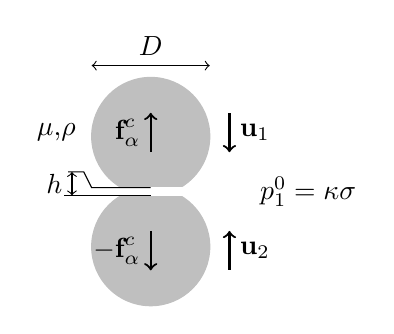
\begin{tikzpicture}
      \draw[lightgray,fill = lightgray] (0,0.7) circle (0.75);
      \draw[lightgray,fill = lightgray] (0,-0.7) circle (0.75);
      \draw[white,fill=white] (-0.75,-0.05) rectangle (0.75,0.05);
      \draw(0,0.05)--++(-0.75,0)--++(-0.1,0.2)--++(-0.2,0);
      \draw(0,-0.05)--++(-1.1,0);
      \draw[<->](-1,-0.05) --++ (0,0.3)node[midway,left]{$h$};
      \draw[<->](-0.75,1.6)--++(1.5,0)node[midway,above]{$D$};
      \node (para) at (-1.2,0.75){$\mu$,$\rho$};
      \node (pressure) at (2,0){$p_1^0 = \kappa \sigma$};
      \draw[->,thick](0,0.5)--++(0,0.5)node[midway,left]{$\textbf{f}_\alpha^\text{c}$};
      \draw[->,thick](0,-0.5)--++(0,-0.5)node[midway,left]{$-\textbf{f}_\alpha^\text{c}$};
      \draw[<-,thick](1,0.5)--++(0,0.5)node[midway,right]{$\textbf{u}_1$};
      \draw[<-,thick](1,-0.5)--++(0,-0.5)node[midway,right]{$\textbf{u}_2$};
    \end{tikzpicture}
    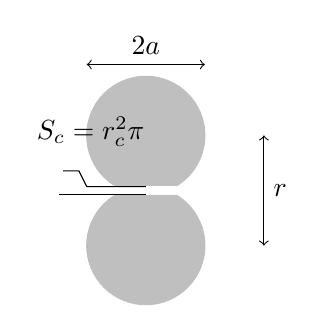
\begin{tikzpicture}
      \draw[lightgray,fill = lightgray] (0,0.7) circle (0.75);
      \draw[lightgray,fill = lightgray] (0,-0.7) circle (0.75);
      \draw[white,fill=white] (-0.75,-0.05) rectangle (0.75,0.05);
      \draw(0,0.05)--++(-0.75,0)--++(-0.1,0.2)--++(-0.2,0);
      \draw(0,-0.05)--++(-1.1,0);
      \draw[<->](-0.75,1.6)--++(1.5,0)node[midway,above]{$2 a$};
      \draw[<->](1.5,0.7)--++(0,-1.4)node[midway,right]{$r$};
      \node (para) at (-0.7,0.75){$S_c = r_c^2 \pi$};
    \end{tikzpicture}
    \caption{Scheme of two colliding droplets at close contact. Note the null kurvature in the region of the interface close to the film leading to a capilary force $\textbf{f}_\alpha^\text{c} \approx - S_c \kappa \sigma \textbf{r}/|\textbf{r}|$. }
\end{figure}

Let use the following notation $(\bm{\sigma}_1' \cdot \textbf{n}_1)^\Sigma = \textbf{f}_\alpha = \textbf{f}_\alpha^\text{h}+\textbf{f}_\alpha^\text{c}$. 
It is clear, since the mean stress contribution $\div \bm{\sigma}_1$ isn't taken in account inside the drag force term, that the contribution $\textbf{f}_\alpha^\text{h}$ vanish or is negligible compared to $\textbf{f}_\alpha^\text{c}$ when the nearest particle is at a distance $|\textbf{r}| < a$ where $a$ is the.  Radius. 

If there is strong inhomogeneous structure in the flow the pure drag force term might be modified to yields the particle fluid particle stress. 
\begin{align*}
    n_p (\bm{\sigma}_1' \cdot \textbf{n}_1)_p^\Sigma
    &= 
    \int_{\mathrm{R}^3} (\bm{\sigma}_1' \cdot \textbf{n}_1)_\text{nst}^\Sigma
    P_\text{nst}(\textbf{x}\pm\textbf{r}/2,\mp\textbf{r}) d\textbf{r}
    +\div \int_{\mathrm{R}^3} \textbf{r} (\bm{\sigma}_1' \cdot \textbf{n}_1)_\text{nst}^\Sigma
    P_\text{nst}(\textbf{x},\textbf{r}) d\textbf{r}\\
\end{align*}
Which can be again decomposed into : 
\begin{align*}
    n_p (\bm{\sigma}_1' \cdot \textbf{n}_1)_p^\Sigma
    &= 
    \frac{1}{2}\int_{\mathrm{R}^3} \textbf{f}^h_\text{nst}P_\text{nst}(\textbf{x}\pm\textbf{r}/2,\mp\textbf{r}) d\textbf{r}
    + \frac{1}{2}\int_{\mathrm{R}^3} \textbf{f}^c_\text{nst}P_\text{nst}(\textbf{x}\pm\textbf{r}/2,\mp\textbf{r}) d\textbf{r} \\
    &
    +\div \int_{\mathrm{R}^3} \textbf{r} \textbf{f}_\text{nst}^\text{h} P_\text{nst}(\textbf{x},\textbf{r}) d\textbf{r}
    +\div \int_{\mathrm{R}^3} \textbf{r} \textbf{f}_\text{nst}^\text{c} P_\text{nst}(\textbf{x},\textbf{r}) d\textbf{r}\\
\end{align*}
The first term is the pure drag force components. 
The second terms is the pure contact force components which we will see to be null in the next section. 
Then, the third term is the particle-fluid-particle stress. 
And the last is the particle-film-particle stress. 


\subsubsection*{The contact forces}
In the same spirit as the classical surface force, as it is defined in \citet{jackson1997locally,zhang1997momentum,nott2011suspension} we can argue that the ensemble average of the close contact force cancel out. 
More precisely, the contact force on a single particle labeled $i$ due to the close contact with particle $j$ can be modeled by, 
\begin{equation*}
    \textbf{f}_{ij}^\text{c}
    = S_c \kappa \sigma \textbf{r}_{ij}/r_{ij}
    = \pi r_c^2 \kappa \sigma \textbf{r}_{ij}/r_{ij}
    = \pi (a^2 - r_{ij}^2/4) \kappa \sigma  \textbf{r}_{ij}/r_{ij}
\end{equation*} 
The resultants of these forces on the particle $i$ is therefore the sum of the contact with all particles except the $j^\text{th}$ particle, 
\begin{equation*}
    \textbf{f}_{i}^\text{c}
    = \sum_{j \neq i}\textbf{f}_{ij}
    = - \sum_{j \neq i} \pi (a^2 - r_{ij}^2/4) \kappa \sigma \textbf{r}_{ij}/r_{ij}
\end{equation*} 
The ensemble average of this force can be written using the classic point particle average,
\begin{align}    
\pavg{\textbf{f}_i^c}
&=
\int \sum_{i} \delta_i 
\textbf{f}_i^c d\PP 
= \int \sum_{i} \sum_{j \neq i} \delta(\textbf{x} - \textbf{x}_i) 
\textbf{f}_{ij}^c d\PP 
\\
\end{align}
Not that $\textbf{f}_{ij} = - \textbf{f}_{ji}$ however $\delta_i \textbf{f}_{ij} \neq - \delta_j\textbf{f}_{ji}$ thus the sum dosen't cancel drictly. 
Thus, following \citet{nott2011suspension,zhang1997momentum} we introduce the sum $\sum_j \delta(\textbf{x}-\textbf{x}_{ij}) \textbf{f}_{ij}^c =0$ where $\textbf{x}_{ij} = \textbf{x}_{ji} = (\textbf{x}_i+\textbf{x}_j)/2$.
Besides, note that, 
\begin{equation*}
    \delta(\textbf{x} - \textbf{x}_{ij})
    = 
    \delta(\textbf{x} - \textbf{x}_i + ( \textbf{x}_{ij} - \textbf{x}_i))
    =
    \delta(\textbf{x} - \textbf{x}_i )
    - ( \textbf{x}_{ij} - \textbf{x}_i)\cdot \grad \delta(\textbf{x}-\textbf{x}_\alpha)
    +\frac{1}{2} (\textbf{x}_{ij} - \textbf{x}_i)(\textbf{x}_{ij} - \textbf{x}_i) : \grad\grad \delta(\textbf{x}-\textbf{x}_\alpha)
\end{equation*}
using both relation yields, 
\begin{align}    
    \pavg{\textbf{f}_i^c}
    &= \int \sum_{i} \sum_{j \neq i} [
        \delta(\textbf{x} - \textbf{x}_i)
        -\delta(\textbf{x} - \textbf{x}_{ij})]
    \textbf{f}_{ij}^c d\PP 
    \\
    &= \div \int \sum_{i} \sum_{j \neq i} \delta(\textbf{x}-\textbf{x}_i) (\textbf{x}_{ij} - \textbf{x}_i)
    \textbf{f}_{ij}^c d\PP 
    \\
    &= \frac{1}{2}\div \int \sum_{i} \sum_{j \neq i} \delta(\textbf{x}-\textbf{x}_i) (\textbf{x}_{j} - \textbf{x}_i)
    \textbf{f}_{ij}^c d\PP 
\end{align}
Using the formula for the contact force gives 
\begin{align}    
    \pavg{\textbf{f}_i^c}
    &= \frac{1}{2}\div \int \sum_{i} \sum_{j \neq i} \delta(\textbf{x}-\textbf{x}_i) 
    \textbf{r}\textbf{r}
    \pi (r^2/4 - a^2) /r \kappa \sigma d\PP 
    \\
\end{align}


\subsubsection*{Nearest stats for contacts forces in dilute case}
In the dilute case we consider only one conatc force so that, 
\begin{equation}
    n_p \textbf{f}^c_p = \iint 
    \sum_i 
    \delta(\textbf{x} -\textbf{x}_i)
    \sum_k 
    \textbf{f}_{k \to i}^\text{c} 
    \sum_{j\neq i}
    \delta(\textbf{x} + \textbf{r} -\textbf{x}_j) h_{ij}(t,\CC)
    d\PP d\textbf{r}\\
\end{equation}
Now we make use of a trick to cancel the pair particles forces by notticing that, 
\begin{equation}
    n_p \textbf{f}^c_p = \iint 
    \sum_k 
    \delta(\textbf{x} -\textbf{x}_k)
    \sum_i
    \textbf{f}_{i\to k}^\text{c} 
    \sum_{j\neq k}
    \delta(\textbf{x} + \textbf{r} -\textbf{x}_j) h_{kj}(t,\CC)
    d\PP d\textbf{r}\\
\end{equation}
So, we have, 
\begin{equation}
    n_p \textbf{f}^c_p = \frac{1}{2}\iint 
    \sum_i 
    \sum_k 
    \left[
        \sum_{j\neq i}
        \delta(\textbf{x} -\textbf{x}_i)
        \delta(\textbf{x} + \textbf{r} -\textbf{x}_j) h_{ij}
        \textbf{f}_{k \to i}^\text{c} 
        +
        \sum_{j\neq k}
        \delta(\textbf{x} -\textbf{x}_k)
        \delta(\textbf{x} + \textbf{r} -\textbf{x}_j) h_{kj}
        \textbf{f}_{i \to k}^\text{c} 
    \right]
    d\PP d\textbf{r}\\
\end{equation}
Note that the sums do not have the same restrictions. 
Nevertheless, this can be neglected since, if for example, $j=i$ we obtain $\delta(\textbf{x}-\textbf{x}_i)\delta(\textbf{x}+\textbf{r}-\textbf{x}_i) = 0$ thus the term cancel unless $\textbf{r}=0$ but let neglect that.
Besides, we must define manually that $h_{ii} = 0$ but it doesn't really matter.   
Or we get out these specifics case such as,
\begin{align}
    n_p \textbf{f}^c_p 
    &= \frac{1}{2}\iint 
    \sum_i 
    \sum_k 
    \sum_{j\neq k,i}
    \left[
        \delta(\textbf{x} -\textbf{x}_i)
        \delta(\textbf{x} + \textbf{r} -\textbf{x}_j) h_{ij}
        \textbf{f}_{k \to i}^\text{c} 
        +
        \delta(\textbf{x} -\textbf{x}_k)
        \delta(\textbf{x} + \textbf{r} -\textbf{x}_j) h_{kj}
        \textbf{f}_{i \to k}^\text{c} 
    \right]
    d\PP d\textbf{r}\\
    &+ \frac{1}{2}\iint 
    \sum_i 
    \sum_k 
    \left[
        \delta(\textbf{x} -\textbf{x}_i)
        \delta(\textbf{x} + \textbf{r} -\textbf{x}_k) h_{ik}
        \textbf{f}_{k \to i}^\text{c} 
        +
        \delta(\textbf{x} -\textbf{x}_k)
        \delta(\textbf{x} + \textbf{r} -\textbf{x}_i) h_{ki}
        \textbf{f}_{i \to k}^\text{c} 
    \right]
    d\PP d\textbf{r}\\
\end{align}

Now we must verify that this framework is coherent with the nearest particle statistics framework.
First we recall the definition of the pure drag term of the contact forces according to the neaerst particle statistics. 
\begin{align*}
    \pavg{\textbf{f}_i^\text{c}}
    &= \frac{1}{2}\int \nstavg{\textbf{f}_i^\text{c}} P_\text{nst}(\textbf{x}\pm\textbf{r}/2,\mp \textbf{r}) d\textbf{r}\\
    &=
    \frac{1}{2}\iint \sum_i \sum_{j\neq i}
    \delta(\textbf{x} \pm \textbf{r}/2 -\textbf{x}_i) 
    \delta(\textbf{x} \mp \textbf{r} -\textbf{x}_j) h_{ij}
    \textbf{f}_i^\text{c} 
    d\PP d\textbf{r}\\
    &=
    \frac{1}{2}\iint \sum_i \sum_{j\neq i}
    \delta(\textbf{x} \pm \textbf{r}/2 -\textbf{x}_i)
    \delta(\textbf{x} \mp \textbf{r} -\textbf{x}_j) h_{ij}
    \sum_{k} \textbf{f}_{ik}^\text{c} 
    d\PP d\textbf{r}\\
    &=
    \frac{1}{2}\iint \sum_i \sum_{j\neq i}
    \delta(\textbf{x} \pm \textbf{r}/2 -\textbf{x}_i)
    \delta(\textbf{x} \mp \textbf{r} -\textbf{x}_j) h_{ij}
     (\textbf{f}_{ij}^\text{c} + \sum_{k\neq i,j} \textbf{f}_{ik}^c)
    d\PP d\textbf{r}
\end{align*}
We must verify that both component of this integral cancel out. 
Changing teh integration sign we get,
\begin{equation*}
    \int \nstavg{\textbf{f}_i^\text{c}} P_\text{nst}(\textbf{x}, \textbf{r}) d\textbf{r}
    = \int \nstavg{\textbf{f}_i^\text{c}} P_\text{nst}(\textbf{x}, - \textbf{r}) d\textbf{r}
\end{equation*}
The drag force can alse, be written, 
\begin{equation*}
    \int [\textbf{f}^c_\text{eb}(\textbf{x}+\textbf{r}/2,\textbf{x} - \textbf{r}/2)+ \textbf{f}_\text{eb}^c(\textbf{x} -\textbf{r}/2,\textbf{x}+ \textbf{r}/2)]P_2(\textbf{x}\pm\textbf{r}/2,\textbf{x}\mp \textbf{r}/2) d\textbf{r}
    = \\
\end{equation*}
And since the contact force has only an antisymmetric contribution in average it is always true that in an averaged sense we have $\nstavg{\textbf{f}_i^\text{c}} P_\text{nst}(\textbf{x}, \textbf{r})  = - \nstavg{\textbf{f}_i^\text{c}} P_\text{nst}(\textbf{x}, - \textbf{r}) $, 
Additionally, 
\begin{align*}
    \pavg{\textbf{f}_\text{eb}^\text{c}}
    &=
    \frac{1}{2}\iint \sum_i \sum_{j\neq i}
    \delta(\textbf{x} + \textbf{r}/2 -\textbf{x}_i)
    \delta(\textbf{x} - \textbf{r}/2 -\textbf{x}_j) h_{ij}
    \sum_{k \neq i} \textbf{f}_{ik}^\text{c} 
    d\PP d\textbf{r}\\
    &=
    \frac{1}{2}\iint \sum_i \sum_{j\neq i}
    \delta(\textbf{x} + \textbf{r}/2 -\textbf{x}_i)
    \delta(\textbf{x} - \textbf{r}/2 -\textbf{x}_j) 
    h_{ij}
    \sum_{k \neq i} \textbf{f}_{ik}^\text{c} 
    d\PP d\textbf{r}\\
\end{align*}

\begin{align}    
\pavg{\textbf{f}_i^c}
&= \int_{|\textbf{r}|<a}
\int \sum_{i \neq j} \delta_i \sum_{j\neq i} \delta_j h_{ij}
\textbf{f}_i^c d\PP d\textbf{r}
= \int_{|\textbf{r}|<a}
\int \sum_{i \neq j} \delta_i \sum_{j\neq i} \delta_j h_{ij}
\sum_{k\neq i} \pi (r_{ik}^2/4 - a^2) \kappa \sigma \textbf{r}_{ik}/r_{ik} d\PP d\textbf{r}\\
&= \int_{|\textbf{r}|<a}
\int \sum_{i \neq j} \delta_i \sum_{j\neq i} \delta_j h_{ij}
\sum_{k\neq i} \pi (r_{ik}^2/4 - a^2) \kappa \sigma \textbf{r}_{ik}/r_{ik} d\PP d\textbf{r}
\\
\end{align}

Anyhow if we lake the assumption that this term indeed cancel we arrive at the expression: 
\begin{equation*}
    \int_{\mathrm{R}^3} \textbf{r} \textbf{f}_\text{nst}^\text{c} P_\text{nst}(\textbf{x},\textbf{r}) d\textbf{r}
    = 
\end{equation*}

\section{The dumping model}

Let decompose the drag force such that $\textbf{f}_\alpha = \textbf{f}_\alpha^h + \textbf{f}_\alpha^c$ with $^h$ being the hydrodynamical forces and $\textbf{f}^c_\alpha$ being the contatc forces. 
Let assume that the particle $\alpha$ interact with the particle $\beta$, where both particles has a radius $a$.
Let note $\textbf{r} = (\textbf{x}_\alpha - \textbf{x}_\beta) = \textbf{n} a$. 
Now let consider that the contact force can be modeled as a spring/dumping model with $k$ being the \textit{Raideur} and $c$ the dumping coefficient.
Then, the contact force between both particles can be written as, 
\begin{equation}
    \textbf{f}_\beta^c
    = \textbf{f}_{\alpha\beta}
    = (|\textbf{r}| - a) \textbf{n} k 
    + (\textbf{u}_\alpha - \textbf{u}_\beta) c
    \;\;\;\;\text{for} \;\;\; (|\textbf{r}| - a) < 0
\end{equation}
For smooth particle the second term can be reduced to the components along the normal vector \textbf{n}.  
Due to Newton's  law and since each interaction force cancel each other we have $\avg{\textbf{f}_\beta^c} \approx 0$. 
However, it is useful to note that we have in the case of inhomogeneous scenario $\avg{\textbf{f}_\beta^c} \approx - \div \Sigma^c$.

Now let's focus on the source term of the granular temperature $\avg{\textbf{f}_\alpha\cdot \textbf{u}_\alpha'} = \avg{\textbf{f}_\alpha^h \cdot \textbf{u}_\alpha'} + \avg{\textbf{f}_\alpha^c\cdot \textbf{u}_\alpha'}$. 
The first source term $\avg{\textbf{f}_\alpha^h \cdot \textbf{u}_\alpha'} \sim k_p$ since $\textbf{f}_\alpha \sim \textbf{u}_\alpha$.

The part due to collision can be re written using the nearest averaged statistics formalism, 
\begin{align*}
    \avg{\textbf{f}_\alpha^c\cdot \textbf{u}_\alpha'}
    &= \int_{\textsc{R}^3}
    \int \sum_{\alpha \neq \beta} \delta_\alpha \delta_\beta h_{\alpha\beta}
    \textbf{u}'_\alpha \textbf{f}_\alpha^c d\PP d\textbf{r}\\
    &= \int_{\textsc{R}^3}
    \int \sum_{\alpha \neq \beta} \delta_\alpha \delta_\beta h_{\alpha\beta}
    \textbf{u}'_\alpha \cdot \textbf{n}
        (|\textbf{r}| - a) 
     d\PP d\textbf{r}
    + \int_{\textsc{R}^3}
    \int \sum_{\alpha \neq \beta} \delta_\alpha \delta_\beta h_{\alpha\beta}
    \textbf{u}'_\alpha 
         (\textbf{u}_\alpha - \textbf{u}_\beta) c
     d\PP d\textbf{r}\\
    &=k \int_{|\textbf{r}|<a}
    \nstavg{\textbf{u}'_\alpha \cdot \textbf{n}
        (|\textbf{r}| - a)   }
        P_{nst}(\textbf{x},\textbf{r})
     d\textbf{r}
    +c \int_{|\textbf{r}|<a}
        \nstavg{\textbf{u}'_\alpha 
         \cdot (\textbf{u}_\alpha - \textbf{u}_\beta)} P_\text{nst}(\textbf{x},\textbf{r})
     d\textbf{r}\\
\end{align*}
Elastic collisions are not dissipative therefore the first term cancel by definition. 
Thus, we are left with, 
\begin{align*}
    \avg{\textbf{f}_\alpha^c\cdot \textbf{u}_\alpha'}
    = c \int_{|\textbf{r}|<a}
        \nstavg{\textbf{u}'_\alpha 
         \cdot (\textbf{u}_\alpha - \textbf{u}_\beta)} P_\text{nst}(\textbf{x},\textbf{r})
     d\textbf{r} 
\end{align*}
\subsection{The dispersed phase equations}

Regarding the dispersed phase, we found the mass, momentum and total energy balance equations, 
\begin{align*}
    \pddt \left(n_p m_p\right)
    + \div \left(n_pm_p\textbf{u}_p
    \right)
    = 
    0\\
    \pddt \left(n_p m_p \textbf{u}_p\right)
    + \div \left(n_p
    m_p \textbf{u}_p \textbf{u}_p 
    - \bm{\sigma}_p^\text{eq}
    \right)
    = 
    n_p v_p  (  
    \rho_2 \textbf{g}
    - \grad p_1)
    + n_p (\bm{\sigma}_1'\cdot \textbf{n}_2)_p^\Sigma,\\
    \pddt(m_p n_pE_p^\text{tot})
    + \div(m_pn_p E_p^\text{tot} \textbf{u}_p 
    + \textbf{q}_p^\text{eq} - \textbf{u}_p \cdot \bm{\sigma}_p^\text{eq})
    =  n_p v_p [\rho_2 \textbf{u}_p\cdot  \textbf{g} 
    - \div (\textbf{u}_1 p_1)]\\
    +  n_p ( \textbf{u}'_1 \cdot \bm{\sigma}_1^0 \cdot \textbf{n}_2)_p^\Sigma
    -  n_p (\textbf{q}_1^0 \cdot \textbf{n}_2)_p^\Sigma
    +  n_p (\textbf{u}_1 \cdot \bm{\sigma}_1'\cdot \textbf{n}_2)_p^\Sigma
\end{align*}
where we have defined, 
\begin{align*}
    &\bm{\sigma}_p^\text{eq}
    = -  m_p\pnavg{\textbf{u}_\alpha'\textbf{u}_\alpha'}
    &\textbf{q}_p^\text{eq}
    =\textbf{q}_p^\text{e} 
    +\textbf{q}_p^\text{k}  
    +\textbf{q}_p^\text{w}  
    \\
    &\textbf{q}_1^\text{e}
    = m_p \pnavg{\textbf{u}_\alpha' e_\alpha'} 
    &\textbf{q}_p^\text{k}
    = m_p \pnavg{\textbf{u}_\alpha' k_\alpha} 
    \\
    &\textbf{q}_p^\text{w}
    = 
    + \pnavg{\textbf{u}_\alpha'(\rho_2 (w^0_2)^2/2 )'_\Omega}
    + \gamma \pnavg{\textbf{u}_\alpha' s_\alpha'}
\end{align*}

Now, subtracting each of these equations to the total NRJ equations yields, 


\tb{Think about doing a surface equation ? ? }
At the Lagrangian scale, 
\begin{equation*}
    \pavg{\ddt (m_\alpha E_\alpha + s_\alpha \gamma)}
    = 
     n_p (\rho_2 \textbf{u}_2^0  \cdot \textbf{g})^\Omega_p
    +n_p (\textbf{u}_1^0 \cdot \bm{\sigma}_1^0 \cdot  \textbf{n}_2)^\Sigma_p
    - n_p (\textbf{q}_1^0 \cdot \textbf{n}_2)^\Sigma_p
\end{equation*}
\begin{align}
    \pavg{\frac{1}{2}\ddt (m_\alpha u_\alpha^2)}
    &= 
    n_p (\rho_2 \textbf{u}_2^0 \cdot
    \textbf{g})_p^\Omega
    + 
    (\textbf{u}_\alpha\cdot
    \textbf{f}_\alpha)_p\\
    \pavg{\frac{1}{2}\ddt \left[\int_{\Omega_\alpha} \rho_2 (w_2^0)^2 d\Omega +s_\alpha \gamma\right] }
    &= (\textbf{w}_1^0 \cdot (\bm{\sigma}_1^0 \cdot \textbf{n}_2) )_p^\Sigma  
     - (\bm{\sigma}_2^0 : \grad\textbf{u}_2^0)_p^\Omega  
    \\
    \pavg{\ddt (m_\alpha e_\alpha )}
    &= 
     + n_p (\bm{\sigma}_2^0 : \grad\textbf{u}_2^0)^\Omega_p
    -  n_p (\textbf{q}_1^0 \cdot \textbf{n}_2 )_p^\Sigma
\end{align}
We first note that, 
\begin{equation*}
    n_p\frac{1}{2}(m_\alpha u_\alpha^2)_p
    = n_p\frac{1}{2}m_p u_p^2
    +  k_p
\end{equation*}
Deriving the momentum kinetic NRJ equation for the particle phase and the above else we can have the following system of equations. 
\begin{align*}
    &\pddt \left(n_p m_p u_p^2/ 2\right)
    + \div \left(n_p
    m_p u_p^2/ 2 \textbf{u}_p 
    - \textbf{u}_p \cdot \bm{\sigma}_p^\text{eq}
    \right)
    = 
    - \bm{\sigma}_p^\text{eq}  :\grad \textbf{u}_p
    +  n_p v_p \textbf{u}_p \cdot (
    \rho_2 \textbf{g}
    - \grad p_1 )
    + n_p \textbf{u}_p \cdot (\bm{\sigma}'_1 \cdot \textbf{n}_2)^\Sigma_p,\\
    &\pddt \left(n_p (\rho_2 w^2 )_p^\Omega+\gamma s_p n_p\right)
    + \div 
    (n_p (\rho_2 w^2 )_p^\Omega+\gamma s_p n_p)
    \textbf{u}_p 
    +  \textbf{q}_p^\text{w}
    )
    = \\
    &- n_p (\bm{\sigma}_2^0 : \grad\textbf{u}_2^0)^\Omega_p
    + n_p (\textbf{u}_1 \cdot \bm{\sigma}_1' \cdot  \textbf{n}_2)^\Sigma_p
    + n_p (\textbf{u}_1' \cdot \bm{\sigma}_1^0 \cdot  \textbf{n}_2)^\Sigma_p
    -n_p v_p \grad (\textbf{u}_1p_1)
    - n_p (\textbf{u}_\alpha \cdot \bm{\sigma}_1^0 \cdot  \textbf{n}_2)^\Sigma_p
    \\
    &\pddt \left(n_p m_p e_p\right)
    + \div \left(n_p
    m_p e_p \textbf{u}_p 
    +  \textbf{q}_p^\text{e}
    \right)
    = 
    + n_p (\bm{\sigma}_2^0 : \grad\textbf{u}_2^0)^\Omega_p
    - n_p (\textbf{q}_1^0\cdot \textbf{n}_2)^\Sigma_p\\
\end{align*}

Now if we subtract these from the total NRJ equation one can show, 
\begin{multline*}
    \pddt(m_p n_pk_p)
    + \div(m_pn_p k_p \textbf{u}_p 
    + \textbf{q}_p^\text{k})
    = 
     \bm{\sigma}_p^\text{eq}  :\grad \textbf{u}_p
     + n_p v_p \textbf{u}_p \grad p_1
     + n_p (\textbf{u}_\alpha \cdot \bm{\sigma}_1^0 \cdot  \textbf{n}_2)^\Sigma_p
     - n_p \textbf{u}_p \cdot (\bm{\sigma}_1' \cdot  \textbf{n}_2)^\Sigma_p
    \\
\end{multline*}
Note that, 















In order to be consistent with the fluid phase equations these terms must be written with $\textbf{f}_\text{pm} = n_p\textbf{u}_1 \cdot ((\bm{\sigma}_1^0 \cdot  \textbf{n}_2)^\Sigma_{nst}(\textbf{x} \pm \textbf{r}/2,\mp\textbf{r}) )_p$, and espetially  $\textbf{f}_\text{pm} = n_p ((\textbf{u}_1' \cdot\bm{\sigma}_1^0 \cdot  \textbf{n}_2)^\Sigma_{nst}(\textbf{x} \pm \textbf{r}/2,\pm\textbf{r}))_p$. Thus we need to reformulate. 
We use, 
\begin{align*}
    n_p (\bm{\sigma}_1^0 \cdot  \textbf{n}_2)^\Sigma_p
    = 
    n_p ( \bm{\sigma}_1' \cdot  \textbf{n}_2)^\Sigma_p
    - n_p (p_1   \textbf{n}_2)^\Sigma_p\\
    n_p (\textbf{u}_1^0 \cdot \bm{\sigma}_1^0 \cdot  \textbf{n}_2)^\Sigma_p
    = 
    n_p (\textbf{u}_1 \cdot \bm{\sigma}_1' \cdot  \textbf{n}_2)^\Sigma_p
    + n_p (\textbf{u}_1' \cdot \bm{\sigma}_1^0 \cdot  \textbf{n}_2)^\Sigma_p
    - n_p (\textbf{u}_1 p_1 \cdot  \textbf{n}_2)^\Sigma_p
\end{align*}
Note that $\textbf{u}_1$ and $p_1$ varies slowly inside the volume of the particle.
Consequently we must use the relation, $\textbf{u}_1(\textbf{r}) = \textbf{u}_1(\textbf{x}_\alpha) + \textbf{r} \cdot\grad \textbf{u}_1(\textbf{x}_\alpha) \ldots$
and $p_1(\textbf{r}) = p_1(\textbf{x}_\alpha) + \textbf{r} \cdot\grad p_1(\textbf{x}_\alpha) \ldots$
to finnaly obtain, 
\begin{align*}
    n_p (\bm{\sigma}_1^0 \cdot  \textbf{n}_2)^\Sigma_p
    &= 
    n_p ( \bm{\sigma}_1' \cdot  \textbf{n}_2)^\Sigma_p
    - n_p v_p \grad p_1\\
    n_p (\textbf{u}_1^0 \cdot \bm{\sigma}_1^0 \cdot  \textbf{n}_2)^\Sigma_p
    &= 
    n_p (\textbf{u}_1 \cdot \bm{\sigma}_1' \cdot  \textbf{n}_2)^\Sigma_p
    + n_p (\textbf{u}_1' \cdot \bm{\sigma}_1^0 \cdot  \textbf{n}_2)^\Sigma_p
    - n_p v_p \div (\textbf{u}_1 p_1) \\
    &= 
    n_p \textbf{u}_1 \cdot( \bm{\sigma}_1' \cdot  \textbf{n}_2)^\Sigma_p
    + n_p (\textbf{r} \bm{\sigma}_1' \cdot  \textbf{n}_2)^\Sigma_p : \grad \textbf{u}_1
    + n_p (\textbf{u}_1' \cdot \bm{\sigma}_1^0 \cdot  \textbf{n}_2)^\Sigma_p
    - n_p v_p \div (\textbf{u}_1 p_1) \\
    &= 
    n_p \textbf{u}_1 \cdot \textbf{f}_{pm}
    + n_p (\mathcal{F}_p - \mathcal{F}_\text{pfp}): \grad \textbf{u}_1
    + n_p \textbf{c}_\text{pm}
    + \div [n_p(\mathcal{C}_\text{pfp} + \textbf{u}_1 \cdot \mathcal{F}_\text{pfp})]
    - n_p v_p \div (\textbf{u}_1 p_1) 
\end{align*}

\begin{align*}
    n_p (\textbf{w}_1^0 \cdot \bm{\sigma}_1^0 \cdot  \textbf{n}_2)^\Sigma_p
    &= 
    n_p (\textbf{u}_1^0 \cdot \bm{\sigma}_1^0 \cdot  \textbf{n}_2)^\Sigma_p
    - n_p (\textbf{u}_\alpha \cdot \bm{\sigma}_1^0 \cdot  \textbf{n}_2)^\Sigma_p\\
    n_p (\textbf{u}_\alpha \cdot \bm{\sigma}_1^0 \cdot  \textbf{n}_2)^\Sigma_p
    &=
    n_p (\textbf{u}_\alpha \cdot \bm{\sigma}_1' \cdot  \textbf{n}_2)^\Sigma_p
    - n_p (\textbf{u}_\alpha \cdot p_1 \cdot  \textbf{n}_2)^\Sigma_p
    % n_p (\textbf{u}_1 \cdot \bm{\sigma}_1' \cdot  \textbf{n}_2)^\Sigma_p
    % + n_p (\textbf{u}_1' \cdot \bm{\sigma}_1^0 \cdot  \textbf{n}_2)^\Sigma_p
    % - n_p v_p \div (\textbf{u}_1 p_1) \\
\end{align*}

In fact if we start back from the exact relation defined in the continuous pahse we can say that ,
\begin{align*}
    \avg{\delta_I (\bm{\sigma}_1^0 ) \textbf{n}_2} - p_1 \grad \phi_1
    = 
    % \avg{\delta_I (\bm{\sigma}_1^0 + p_1)\cdot \textbf{n}_2}
    % = 
    \avg{\delta_I \bm{\sigma}_1'\cdot \textbf{n}_2}
    \\
    \avg{\delta_I (\textbf{u}_1^0 \cdot\bm{\sigma}_1^0 )} - \textbf{u}_1p_1\cdot \grad \phi_1
    % = \avg{\delta_I (\textbf{u}_1 \cdot \bm{\sigma}_1' + \textbf{u}_1' \cdot \bm{\sigma}_1^0 )\cdot \textbf{n}_2}
    = \textbf{u}_1 \cdot \avg{\delta_I \bm{\sigma}_1'\cdot \textbf{n}_2}
    + \avg{\delta_I (\textbf{u}_1' \cdot \bm{\sigma}_1^0 )\cdot \textbf{n}_2}
\end{align*}

incoherence in teh exchange terms, 
\begin{align*}
    n_p (\textbf{u}_\alpha' \cdot \bm{\sigma}_1^0\cdot \textbf{n}_2)^\Sigma_p
    &= \int
    \sum_\alpha \delta_\alpha(\textbf{x} - \textbf{x}_\alpha)
    \textbf{u}_\alpha'(\CC,t)\cdot
    \left[\int_{\Sigma_\alpha} 
     (\bm{\sigma}_1^0 +p_1 \textbf{I})\cdot \textbf{n}_2
     d\textbf{r}
    - \int_{\Sigma_\alpha} 
     p_1  \textbf{n}_2
     d\textbf{r}\right]
     d\PP \\
    &= \int
    \sum_\alpha \delta_\alpha(\textbf{x} - \textbf{x}_\alpha)
    \textbf{u}_\alpha'(\CC,t)\cdot
    \left[\int_{\Sigma_\alpha} 
     \bm{\sigma}_1' +\cdot \textbf{n}_2
     d\textbf{r}
    - v_\alpha \grad p_1(\textbf{x}_\alpha)
    \right]
     d\PP \\
    &= n_p (\textbf{u}_\alpha' \cdot (\bm{\sigma}'_1\cdot \textbf{n}_2)^\Sigma )_p
    -  n_p (\textbf{u}_\alpha' v_p \cdot \grad p_1 )_p
     \\
    &= n_p (\textbf{u}_\alpha' \cdot (\bm{\sigma}'_1\cdot \textbf{n}_2)^\Sigma )_p
     \\
\end{align*}
Since $\textbf{u}_p$ is an Eulerian fields it must be evaluated at $\textbf{r}$ Therefore it must get out the 

Also, 
\begin{align*}
    n_p (\textbf{u}_1' \cdot \bm{\sigma}_1'\cdot \textbf{n}_2)^\Sigma_p
    &= \int
    \sum_\alpha \delta_\alpha(\textbf{x} - \textbf{x}_\alpha)
    \left[\int_{\Sigma_\alpha} 
    \textbf{u}_1'\cdot
    \bm{\sigma}_1^0\cdot \textbf{n}_2
    d\textbf{r}
    + \int_{\Sigma_\alpha} 
    \textbf{u}_1'\cdot
     p_1  \textbf{n}_2
     d\textbf{r}\right]
     d\PP \\
    &= n_p (\textbf{u}_1' \cdot \bm{\sigma}_1^0 \cdot \textbf{n}_2)^\Sigma_p
    -  n_p (\textbf{u}_1'[p_1  +  \textbf{r}\cdot \grad p_1 ]\cdot \textbf{n}_2 )_p^\Sigma
     \\
    &= n_p (\textbf{u}_1' \cdot \bm{\sigma}_1^0 \cdot \textbf{n}_2)^\Sigma_p
    -  n_p p_1  (\div \textbf{u}_1')_p^\Omega
    -  n_p (\textbf{u}_1'[p_1  +  \textbf{r}\cdot \grad p_1 ]\cdot \textbf{n}_2 )_p^\Sigma\\
    &= n_p (\textbf{u}_1' \cdot \bm{\sigma}_1^0 \cdot \textbf{n}_2)^\Sigma_p
    -  n_p\grad p_1\cdot ( \textbf{u}'_1)_p^\Omega
     \\
\end{align*}

Also, 
\begin{align*}
    n_p (\textbf{w}_2^0 \cdot \bm{\sigma}_1^0\cdot \textbf{n}_2)^\Sigma_p
    &= \int
    \sum_\alpha \delta_\alpha(\textbf{x} - \textbf{x}_\alpha)
    \cdot
    \left[\int_{\Sigma_\alpha} 
     \textbf{w}_2^0 (\bm{\sigma}_1^0 +p_1 \textbf{I})\cdot \textbf{n}_2
     d\textbf{r}
    - \int_{\Sigma_\alpha} 
     \textbf{w}_2^0 p_1  \textbf{n}_2
     d\textbf{r}\right]
     d\PP \\
    &= \int
    \sum_\alpha \delta_\alpha(\textbf{x} - \textbf{x}_\alpha)
    \left[\int_{\Sigma_\alpha} 
     \textbf{w}_2^0 \cdot \bm{\sigma}_1'\cdot \textbf{n}_2
     d\textbf{r}
    - \int_{\Sigma_\alpha} 
     \textbf{w}_2^0 (p_1 + \textbf{r}\grad p_1)   \textbf{n}_2
     d\textbf{r}\right]
     d\PP \\
     &= n_p (\textbf{w}_2^0 \cdot \bm{\sigma}_1' \cdot \textbf{n}_2)^\Sigma_p
    - n_p (p_1 \textbf{w}_2^0 \cdot \textbf{n}_2)^\Sigma_p\\
     &= n_p (\textbf{w}_2^0 \cdot \bm{\sigma}_1' \cdot \textbf{n}_2)^\Sigma_p
    - n_p (p_1 (\textbf{w}_2^0 \cdot \textbf{n}_2)^\Sigma)_p
    - n_p (\grad p_1\cdot ( \textbf{r} \textbf{w}_2^0 \cdot \textbf{n}_2)^\Sigma)_p\\
     &= n_p (\textbf{w}_2^0 \cdot \bm{\sigma}_1' \cdot \textbf{n}_2)^\Sigma_p
    - n_p (\grad p_1\cdot ( \div(\textbf{r} \textbf{w}_2^0))^\Omega)_p\\
     &= n_p (\textbf{w}_2^0 \cdot \bm{\sigma}_1' \cdot \textbf{n}_2)^\Sigma_p
    - n_p (\grad p_1\cdot ( \div\textbf{r} \textbf{w}_2^0)^\Omega)_p
    - n_p (\grad p_1\cdot ( \textbf{r} \div\textbf{w}_2^0)^\Omega)_p\\
     &= n_p (\textbf{w}_2^0 \cdot \bm{\sigma}_1' \cdot \textbf{n}_2)^\Sigma_p
\end{align*}







The averaged particle energy $n_p E_p$ can be split into five components,
\begin{equation*}
    n_p m_p E_p(t) 
    = m_p n_p e_p 
    + \pnavg{\int_{\Omega_\alpha(t)} \rho_2  (w_2^0)^2/2 d\Omega}
    + m_p n_p k_p
    + m_p n_p (u_p)^2/2
    + n_p s_p \gamma
    % + \textbf{u}_\alpha \cdot \int_{\Omega_\alpha(t)} \rho_2  \textbf{w}_2^0 d\Omega
\end{equation*}
where $k_p = \pavg{(u_\alpha')^2/2}$.
one equation for each is riquiered 
Using the mass balance and the momentum balance dotted with $\textbf{u}_p$ we obtain the particle kinetic energy balance, 
\begin{align*}
    \pddt \left(n_p m_p u_p^2/ 2\right)
    + \div \left(n_p
    m_p u_p^2/ 2 \textbf{u}_p 
    - \textbf{u}_p \cdot \bm{\sigma}_p^\text{eq}
    \right)
    = 
    - \bm{\sigma}_p^\text{eq}  :\grad \textbf{u}_p
    +  n_p v_p \textbf{u}_p \cdot (
    \rho_2 \textbf{g}
    - \grad p_1 )
    + n_p \textbf{u}_p \cdot \textbf{f}_{pm},\\
    \pddt \left(n_p (\rho_2 w^2 )_p^\Omega+\gamma s_p n_p\right)
    + \div 
    (n_p (\rho_2 w^2 )_p^\Omega+\gamma s_p n_p)
    \textbf{u}_p 
    +  \textbf{q}_p^\text{w}
    )
    = 
    - n_p \textbf{d}_p
    +  n_p (\textbf{u}_1 -\textbf{u}_p) \cdot  (\textbf{f}_{pm} - v_p \grad p_1)
    + n_p\textbf{c}_p\\
    \pddt \left(n_p m_p e_p\right)
    + \div \left(n_p
    m_p e_p \textbf{u}_p 
    +  \textbf{q}_p^\text{e}
    \right)
    = 
    + n_p \textbf{d}_p
    + n_p \textbf{e}_{pm},\\
\end{align*}
\tb{we remark that the collision tensor appear exactly at the same place as the pfp}
Subtracting all 3 equation to the total energy finally gives, 
\begin{align*}
    \pddt(m_p n_pk_p)
    + \div(m_pn_p k_p \textbf{u}_p 
    + \textbf{q}_p^\text{k})
    = 
    \bm{\sigma}_p^\text{eq} : \grad \textbf{u}_p
    % - n_p \textbf{d}_p
    - n_p v_p p_1 \div \textbf{u}_1
    + n_p (( \textbf{u}_\alpha' \cdot \bm{\sigma}_1^0 \cdot \textbf{n}_2)^\Sigma_\text{nst}(\textbf{x}\pm\textbf{r}/2,\mp\textbf{r}) )_p^r \\
\end{align*}
The transfer term of the internal droplets' fluctuation reads, 
\begin{align*}
    \int_{\Sigma_\alpha} \textbf{w}_1^0 \cdot (\bm{\sigma}_1^0 \cdot \textbf{n}_2) d\Sigma  
    = 
    (\textbf{u}_1 -\textbf{u}_\alpha) \cdot \int_{\Sigma_\alpha}  (\bm{\sigma}_1^0 \cdot \textbf{n}_2) d\Sigma  
    + \int_{\Sigma_\alpha} \textbf{u}_1' \cdot (\bm{\sigma}_1^0 \cdot \textbf{n}_2) d\Sigma  
    = (\textbf{u}_1 -\textbf{u}_\alpha) \cdot  (\textbf{f}_\alpha - \grad p_1)
    + \textbf{c}_\alpha
\end{align*}
\begin{align*}
    n_p (\textbf{w}_1^0 \cdot \bm{\sigma}_1^0 \cdot \textbf{n}_2)^\Sigma_p
    &= 
    n_p ((\textbf{w}_1^0 \cdot \bm{\sigma}_1^0 \cdot \textbf{n}_2)^\Sigma_\text{nst}(\textbf{x}\pm\textbf{r}/2,\mp\textbf{r}) )_p^r 
    + \div (n_p ( \textbf{r}(\textbf{w}_1^0 \cdot \bm{\sigma}_1^0 \cdot \textbf{n}_2)^\Sigma_\text{nst}(\textbf{x},\textbf{r}) )_p^r )\\
    &= 
    n_p (((\textbf{u}_1-\textbf{u}_\alpha) \cdot \bm{\sigma}_1^0 \cdot \textbf{n}_2)^\Sigma_\text{nst}(\textbf{x}\pm\textbf{r}/2,\mp\textbf{r}) )_p^r 
    +n_p ((\textbf{u}_1' \cdot \bm{\sigma}_1^0 \cdot \textbf{n}_2)^\Sigma_\text{nst}(\textbf{x}\pm\textbf{r}/2,\mp\textbf{r}) )_p^r \\
    &+ \div [n_p ( \textbf{r}((\textbf{u}_1 - \textbf{u}_\alpha) \cdot \bm{\sigma}_1^0 \cdot \textbf{n}_2)^\Sigma_\text{nst}(\textbf{x},\textbf{r}) )_p^r 
    + n_p ( \textbf{r}(\textbf{u}_1' \cdot \bm{\sigma}_1^0 \cdot \textbf{n}_2)^\Sigma_\text{nst}(\textbf{x},\textbf{r}) )_p^r ]\\
    &= 
    n_p (((\textbf{u}_1-\textbf{u}_\alpha) \cdot \bm{\sigma}_1^0 \cdot \textbf{n}_2)^\Sigma_\text{nst}(\textbf{x}\pm\textbf{r}/2,\mp\textbf{r}) )_p^r 
    +n_p \textbf{c}_{pm} \\
    &+ \div [n_p ( \textbf{r}((\textbf{u}_1 - \textbf{u}_\alpha) \cdot \bm{\sigma}_1^0 \cdot \textbf{n}_2)^\Sigma_\text{nst}(\textbf{x},\textbf{r}) )_p^r 
    + n_p \mathcal{C}_\text{pfp}]\\
\end{align*}
The remaining terms can be expressed as, 
\begin{align*}
    n_p (((\textbf{u}_1-\textbf{u}_\alpha) \cdot \bm{\sigma}_1^0 \cdot \textbf{n}_2)^\Sigma_\text{nst}(\textbf{x}\pm\textbf{r}/2,\mp\textbf{r}) )_p^r 
    &= 
    n_p (\textbf{u}_1 - \textbf{u}_p) \cdot (( \bm{\sigma}_1^0 \cdot \textbf{n}_2)^\Sigma_\text{nst}(\textbf{x}\pm\textbf{r}/2,\mp\textbf{r}) )_p^r \\
    &- n_p (( \textbf{u}_\alpha' \cdot \bm{\sigma}_1^0 \cdot \textbf{n}_2)^\Sigma_\text{nst}(\textbf{x}\pm\textbf{r}/2,\mp\textbf{r}) )_p^r \\
    &= 
    n_p (\textbf{u}_1 - \textbf{u}_p) \cdot(\textbf{f}_p - \grad p_1) \\
    &- n_p (( \textbf{u}_\alpha' \cdot \bm{\sigma}_1^0 \cdot \textbf{n}_2)^\Sigma_\text{nst}(\textbf{x}\pm\textbf{r}/2,\mp\textbf{r}) )_p^r \\
\end{align*}
The higher moments terms can be expressed as, 
\begin{align*}
    n_p (\textbf{r}((\textbf{u}_1-\textbf{u}_\alpha) \cdot \bm{\sigma}_1^0 \cdot \textbf{n}_2)^\Sigma_\text{nst})_p^r 
    &= 
    n_p (\textbf{u}_1 - \textbf{u}_p) \cdot (\textbf{r} ( \bm{\sigma}_1^0 \cdot \textbf{n}_2)^\Sigma_\text{nst} )_p^r 
    - n_p ( \textbf{r} ( \textbf{u}_\alpha' \cdot \bm{\sigma}_1^0 \cdot \textbf{n}_2)^\Sigma_\text{nst} )_p^r \\
    &= 
    n_p (\textbf{u}_1 - \textbf{u}_p)\cdot \mathcal{F}_\text{pfp} 
    - n_p (\textbf{r} ( \textbf{u}_\alpha' \cdot \bm{\sigma}_1^0 \cdot \textbf{n}_2)^\Sigma_\text{nst} )_p^r \\
\end{align*}
Alternatively, without the nearest particle formalism we obtain, 
\begin{align*}
    n_p (\textbf{w}_1^0 \cdot \bm{\sigma}_1^0 \cdot \textbf{n}_2)^\Sigma_p
    &= 
    n_p ((\textbf{w}_1^0 \cdot \bm{\sigma}_1^0 \cdot \textbf{n}_2)^\Sigma)_p 
\end{align*}

Averaging the microscopic 
\begin{align}
    \frac{1}{2}\ddt (m_\alpha u_\alpha^2)
    &= 
    \textbf{u}_\alpha\cdot
    \textbf{g}m_\alpha
    + 
    \textbf{u}_\alpha\cdot
    \textbf{f}_\alpha\\
    \frac{1}{2}\ddt \int_{\Omega_\alpha} \rho_2 (w_2^0)^2 d\Omega 
    + \ddt (s_\alpha \gamma) 
    &= 
    \int_{\Sigma_\alpha} \textbf{w}_1^0 \cdot (\bm{\sigma}_1^0 \cdot \textbf{n}_2) d\Sigma  
     - \int_{\Omega_\alpha} \bm{\sigma}_2^0 : \grad\textbf{u}_2^0 d\Omega  
    \\
    \ddt (m_\alpha e_\alpha )
    &= 
     \int_{\Omega_\alpha} \bm{\sigma}_2^0 : \grad\textbf{u}_2^0 d\Omega  
    -  s_\alpha \textbf{q}_\alpha  
\end{align}
Additionally, we can add an equation for the first moment of momentum, 
\begin{multline}
    \pddt \left(n_p \mathcal{P}_p\right)
    + \div \left(
        n_p \textbf{u}_p \mathcal{P}_p
    + \Sigma_p^\text{eq}
    \right)
    =
    n_p v_p \bm{\sigma}_1 
    + n_p \mathcal{F}_p\\
    +\pnavg{\int_{\Omega_\alpha} \left(
        \rho_2 \textbf{w}_2^0  \textbf{w}_2^0 
        - \bm{\sigma}_2^0
        \right) d\Omega}
        - \gamma  \pnavg{\int_{\Sigma_\alpha} \textbf{I}_{||} d\Sigma},
\end{multline}



\subsubsection{Modeling of collisions}

Even through we do not consider pure contact between interfaces it is still indispensable to define some kind of collision with the framework of the hybrid model. 
A contact mediated by the fluid is still different from near close contact, since in the latter case it is capillary pressure that drives the interaction forces. 

\subsection*{The drag force term}

The drag force term is easily closed by numerical method and some theoretical developments in the limiting case. 
Let now study the stokes 

\subsection*{Stress tensor for the continuous phase }
Regarding the fluid stress it can be reformulated considering Newtonian fluid,
\begin{equation}
    \phi_1 \bm{\sigma}_1 
    = - \phi_1 p_1 \textbf{I}
    + \mu_1 \phi_1 \textbf{e}_1
\end{equation}
with $\textbf{e}_1$ being the averaged shear rate. 
The first model is then, 
\begin{align*}
    \phi_1 \textbf{e}_1
    = \phi_1 (\nabla \textbf{u}_1+ (\grad \textbf{u}_1)^T)
    + \avg{[(\textbf{u}_1^0 - \textbf{u}_1)  \textbf{n}_1 +  \textbf{n}_1(\textbf{u}_1^0 - \textbf{u}_1 )]\delta_I}
\end{align*}
In \citet[chap 9]{ishii1975thermo} they assume,
\begin{equation}
    \avg{[(\textbf{u}_1^0 - \textbf{u}_1)  \textbf{n}_1 +  \textbf{n}_1(\textbf{u}_1^0 - \textbf{u}_1 )]\delta_I}\\
    = 
    (\textbf{u}_2 - \textbf{u}_1)  \grad \phi_1 +  \grad \phi_1(\textbf{u}_2 - \textbf{u}_1 )\\
\end{equation}
But I didn't find out where the derivation came from. 
Alternatively we can say that, 
\begin{align*}
    \phi_1 \textbf{e}_1
    = \nabla \textbf{u}+ (\grad \textbf{u})^T
    - \avg{\chi_2 (\grad\textbf{u}_2^0 + \grad(\textbf{u}_2^0 )^T)}
    = \textbf{e}
    - \phi_2 \textbf{e}_2
\end{align*}

More generally the stress within a suspension can be written,
\begin{align*}
    \bm{\sigma}_1 \phi_1
    &=- \phi_1 p_1 \textbf{I}
    + \mu_1 \textbf{e}
    - \lambda \phi_2 \bm{\tau}_2\\
    \bm{\sigma}_1 
    &= - \left(p_1 + \frac{\lambda \phi_2}{\phi_1} p_2\right) \textbf{I}
    + \frac{\mu_1}{\phi_1} \textbf{e}
    - \frac{\lambda \phi_2}{\phi_1} \bm{\sigma}_2\\
    \bm{\sigma}
    &= - \phi_1 p_1  \textbf{I}
    + \mu_1 \textbf{e}
    + \bm{\sigma}_2 \phi_2 
    +\phi_I \bm{\sigma}_I 
    - \lambda \phi_2 \bm{\tau}_2
\end{align*}
We can reformulate the last expression in the usual way using the first moment of momentum eq, 
\begin{equation}
    -  \dot{\mathcal{P}_p}
    +  \mathscr{S}_p^*
    +  \mathscr{L}_p
    + \frac{1}{3}(\bm{\sigma}_1^0 \cdot \textbf{n}_2 \cdot \textbf{r})_p^\Sigma \textbf{I}
    + n_p (\rho_2 \textbf{w}_2^0  \textbf{w}_2^0 )^\Omega
    =   (\bm{\sigma}_2^0)^\Omega
    + (\bm{\sigma}_I)^\Sigma,
\end{equation}
Or in stokes condition, 
\begin{equation}
    n_p \mathscr{S}_p^*
+ n_p \mathscr{L}_p
+ n_p\frac{1}{3}(\bm{\sigma}_1^0 \cdot \textbf{n}_2 \cdot \textbf{r})_p^\Sigma \textbf{I}
    = n_p \left(
        \bm{\sigma}_2^0
    \right)_p^\Omega
    +n_p (\bm{\sigma}_I)^\Sigma_p
\end{equation}
where we defined, 
\begin{align*}
    \mathscr{S}_p^* =\frac{1}{2} \pnavg{\int_{\Sigma_\alpha} \left(
        \textbf{r} \bm{\sigma}_1^0 \cdot \textbf{n}_2
        +  \bm{\sigma}_1^0 \cdot \textbf{n}_2\textbf{r}
        -
          \frac{2}{3}(\bm{\sigma}_1^0 \cdot \textbf{n}_2 \cdot \textbf{r})\textbf{I}
        \right)  d\Sigma}\\
    \mathscr{L}_p =\frac{1}{2} \pnavg{\int_{\Sigma_\alpha} \left(
        \textbf{r} \bm{\sigma}_1^0 \cdot \textbf{n}_2
        - \bm{\sigma}_1^0 \cdot \textbf{n}_2\textbf{r}
        \right) d\Sigma}
\end{align*}
Thus in homogeneous suspension without inertia we have, 
\begin{align*}
    \bm{\sigma}
    &= [- \phi_1 p_1 
    + n_p (\bm{\sigma}_1^0 \cdot \textbf{n}_2 \cdot \textbf{r})^\Sigma_p] \textbf{I}
    + \mu_1 \textbf{e}
    + n_p \mathscr{S}
    + n_p \mathscr{L}
\end{align*}
where the stress let is defined as $\mathscr{S} = \mathscr{S}_p^* - \lambda \phi_2 \bm{\tau}_2$. 
The equivalent stress in the fluid phase averaged equation can be reformulated as, 
\begin{align*}
    \bm{\sigma}_1^\text{eq}
    = \phi_1(
    \bm{\tau}_1%- n_p \textbf{M}_p
    - \rho_1 
    \kavg{\textbf{u}_1'\textbf{u}_1'})
    - n_p \mathcal{F}_\text{pfp} + n_p \mathcal{F}_p
    &= - (\phi_1 \rho_1  \kavg{\textbf{u}_1'\textbf{u}_1'}
        + n_p \mathcal{F}_\text{pfp})
        + \mu_1 \textbf{e} 
        - \lambda \phi_2 \bm{\tau}_2
         + n_p \mathcal{F}_p\\
    &= - (\phi_1 \rho_1  \kavg{\textbf{u}_1'\textbf{u}_1'}
        + n_p \mathcal{F}_\text{pfp})
        + \mu_1 \textbf{e} 
        - \lambda \phi_2 \bm{\tau}_2
         + n_p \mathscr{S}_p^*
         + n_p \mathscr{L}_p\\
    &= - (\phi_1 \rho_1  \kavg{\textbf{u}_1'\textbf{u}_1'}
        + n_p \mathcal{F}_\text{pfp})
        + \mu_1 \textbf{e} 
         + n_p \mathscr{S}_p
         + n_p \mathscr{L}_p
         + n_p (\bm{\sigma}_1^0 \cdot \textbf{n}_2 \cdot\textbf{r})_p^\Sigma \textbf{I}
\end{align*}
Thus, in the most general way the fluid phase stress can be written as that. 
But the last term must go into the equivalent pressure and that is a major founding. 
For netrally buoyant spherical particles : 
\begin{equation*}
    + n_p (\bm{\sigma}_1^0 \cdot \textbf{n}_2 \cdot\textbf{r})_p^\Sigma \textbf{I}
    = 
    n_p/a (p_1^0 )_p^\Sigma \textbf{I}
\end{equation*}
This, is definitely not trivial but if one wish to compute the first moment dynamical contribution to the suspension the formulas is given by 
\begin{align*}
    n_p \mathscr{S}_p
+ n_p \mathscr{L}_p
+ n_p\frac{1}{3}(\bm{\sigma}_1^0 \cdot \textbf{n}_2 \cdot \textbf{r})_p^\Sigma \textbf{I}
    &= 
    n_p \left(
        \bm{\sigma}_2^0
    \right)_p^\Omega
    +n_p (\bm{\sigma}_I)^\Sigma_p
    - \lambda \phi_2 \bm{\tau}_2\\
    &= 
    - n_p \left(
        p_2^0
    \right)_p^\Omega \textbf{I}
    +n_p (\bm{\sigma}_I)^\Sigma_p
    + n_p (1 - \lambda)\left(
        \mu_2 \textbf{e}_2^0
    \right)_p^\Omega 
\end{align*}
Let take the trace times $\frac{1}{3}$ of this equation, 
\begin{align*}
    \frac{1}{3} n_p(\bm{\sigma}_1^0 \cdot \textbf{n}_2 \cdot \textbf{r})_p^\Sigma 
    = 
    - n_p \left(
        p_2^0
    \right)_p^\Omega 
    +n_p \frac{1}{3}(\bm{\sigma}_I)^\Sigma_p : \textbf{I}
\end{align*}
Now let's substitute this equation into the former one, 
\begin{align*}
    n_p \mathscr{S}_p
+ n_p \mathscr{L}_p
=
    +n_p (\bm{\sigma}_I - \frac{1}{3}(\bm{\sigma}_I : \textbf{I})\text{I})^\Sigma_p
    + n_p (1 - \lambda)\left(
        \mu_2 \textbf{e}_2^0
    \right)_p^\Omega 
\end{align*}

If the particle is spherical, and that we remove the isotropic part on both sides of the equation we obtain 

In the spherical particle case the symmetric part reads, 
\begin{align*}
    n_p \mathscr{S}_p
    &= 
    + n_p (1 - \lambda)\left(
        \mu_2 \textbf{e}_2^0
    \right)_p^\Omega 
\end{align*}
which is false. 

\subsubsection{A translating sphere}
In the dilute stokes regime the disturbance velocity around a droplet can be written, 
\begin{align*}
    u_i^\text{Ext}(\textbf{r})
    = \left(\frac{\delta_{ik}}{r} + \frac{r_ir_k}{r^3}\right)  g_k
    + \left(-\frac{\delta_{ik}}{r^3} + \frac{3r_ir_k}{r^5}\right)  d_k\\
    u_i^\text{In}(\textbf{r})
    = c_i
    + \left(2 r^2 \delta_{ik} - r_ir_k\right) e_k\\
    e_{ik}
    = \mu(
        3 \delta_{ij} r_k 
        + 3 \delta_{kj} r_i
        -2 r_j \delta_{ki}
    )e_j 
\end{align*}
Applying the non deformation at the interface and other shear free condition we find the constant to be, 
\begin{align*}
    &\textbf{g} = \frac{1}{4}\left(\frac{3\lambda + 2}{\lambda +1}\right) a \textbf{U}
    &\textbf{d} = -\frac{1}{4}\left(\frac{\lambda}{\lambda +1}\right) a^3 \textbf{U}\\
    &\textbf{c} = \frac{1}{2}\left(\frac{3\lambda + 3}{\lambda +1}\right) \textbf{U}
    &\textbf{e} = -\frac{1}{2}\left(\frac{1}{\lambda +1}\right) \frac{1}{a^2} \textbf{U}\\
\end{align*}
Let consider isolated particles immersed in a viscous flow in the case $\textbf{u}_1' = \textbf{u}^{Ext}$.

The averaged internal shear rate $\phi_2 \textbf{e}_2$ can be thus estimated through the integral, 
\begin{align*}
    \avg{\chi_2 (\textbf{e}_2^0)_{ik}}
    &= \pavg{\int_{\Omega} \mu(
        3 \delta_{ij} r_k 
        + 3 \delta_{kj} r_i
        -2 r_j \delta_{ki}
    )e_j d\Omega}
    = 0\\
    &+ \div \pavg{\int_{\Omega} \textbf{r}\mu(
        3 \delta_{ij} r_k 
        + 3 \delta_{kj} r_i
        -2 r_j \delta_{ki}
    )e_j d\Omega}
\end{align*}
Also, the stress fields for such a flow is given by, 
\begin{equation*}
    T^G_{ijl} 
    = -6\frac{r_ir_jr_k}{r^5}
\end{equation*}

What about the first moment of momentum of the droplets, 
\begin{align*}
    (\mathcal{P}_p)_{ij}
    = \int_{\Omega} 
    u_i^\text{In} r_j 
    d\Omega
    = \int_{\Omega} 
    (c_i r_j 
    + 2 r^2  r_j e_i - r_i r_k r_j e_k)
    d\Omega
    = 0 
\end{align*}
Where we considered spherical particle with no deformation so it is obviously zero.
\begin{align*}
    (\textbf{w}_2^0 \textbf{w}_2^0)_{ij}^\Omega
    = \int_{\Omega} 
    u_i^\text{In}u_j^\text{In}
    d\Omega
    = \int_{\Omega} 
    ( c_i + \left(2 r^2 \delta_{ik} - r_ir_k\right) e_k)
    ( c_j + \left(2 r^2 \delta_{jl} - r_jr_l\right) e_l)
    d\Omega\\
    = \int_{\Omega} 
    (c_i c_j + c_i e_l (2 r^2 \delta_{jl} - r_jr_l )
    + (2 r^2 \delta_{ik} - r_ir_k)c_j e_k
    +  (2 r^2 \delta_{ik} - r_ir_k)(2 r^2 \delta_{jl} - r_jr_l)e_ke_l
    )
    d\Omega\\
    = c_i c_j v_\alpha
    + e_l c_i (2 \mathcal{M}_{kk} \delta_{jl} - \mathcal{M}_{jl})
    + e_k c_j (2 \mathcal{M}_{kk} \delta_{ik} - \mathcal{M}_{ik})\\
    + e_ke_l (\mathcal{M}_{kkkk}\delta_{ik}\delta_{jl}
    -2\mathcal{M}_{kkjl}\delta_{ik}
    -2\mathcal{M}_{kkik}\delta_{jl}
    + \mathcal{M}_{ikjl}) 
\end{align*}
\tb{problem on the units ; Re compute those Acknowledging that the inertia tensor is in fact completely isotropic}

The iternal energy, 
\begin{align*}
    (\textbf{w}_2^0 \textbf{w}_2^0)_{ii}^\Omega
    = \int_{\Omega} 
    u_i^\text{In}u_i^\text{In}
    d\Omega
    = \int_{\Omega} 
    ( c_i + \left(2 r^2 \delta_{ik} - r_ir_k\right) e_k)
    ( c_i + \left(2 r^2 \delta_{il} - r_ir_l\right) e_l)
    d\Omega\\
    = \int_{\Omega} 
    (c_i c_i + c_i e_l (2 r^2 \delta_{il} - r_ir_l )
    + (2 r^2 \delta_{ik} - r_ir_k)c_i e_k
    +  (2 r^2 \delta_{ik} - r_ir_k)(2 r^2 \delta_{il} - r_ir_l)e_ke_l
    )
    d\Omega\\
    = c_i c_i v_\alpha
    + e_l c_i (2 \mathcal{M}_{kk} \delta_{il} - \mathcal{M}_{il})
    + e_k c_i (2 \mathcal{M}_{kk} \delta_{ik} - \mathcal{M}_{ik})\\
    + e_ke_l (\mathcal{M}_{kkkk}\delta_{ik}\delta_{il}
    -2\mathcal{M}_{kkil}\delta_{ik}
    -2\mathcal{M}_{kkik}\delta_{il}
    + \mathcal{M}_{ikil}) 
\end{align*}


\subsubsection{A drop in shear flow}

The functional form of the internal velocity fields for a droplet immersed in a shear flow is,
\begin{align*}
    u_i^\text{Ext}(\textbf{r})
    = \left(\frac{\delta_{ij} r_l - \delta_{il} r_j - \delta_{jl} r_i}{r^3} 
    + \frac{r_ir_jr_l}{r^5}\right)  d_{jl}\\
    + \left(-3 \frac{\delta_{ij} r_l + \delta_{il} r_j + \delta_{jl} r_i}{r^5} 
    + 15\frac{r_ir_jr_l}{r^7}\right)  p_{jl}\\
    u_i^\text{In}(\textbf{r})
    = \left(- 4 \delta_{ij} r_l  + \delta_{il} r_j + \delta_{jl} r_i\right) f_{jl}\\
    e_{ik}
    = \mu [
        \partial_i \left(- 4 \delta_{kj} r_l  + \delta_{kl} r_j + \delta_{jl} r_k\right) f_{jl} + \partial_k \left(- 4 \delta_{ij} r_l  + \delta_{il} r_j + \delta_{jl} r_i\right) f_{jl} 
    ]\\
    = \mu [
        \left(- 4 \delta_{kj} \delta_{li}  + \delta_{kl} \delta_{ji} + \delta_{jl} \delta_{ki}\right) f_{jl} + \left(- 4 \delta_{ij} \delta_{lk}  + \delta_{il} \delta_{kj} + \delta_{jl} \delta_{ki}\right) f_{jl} 
    ]\\
    = \mu [
        \left(- 4 f_{ki}  + f_{ik} + f_{jj}\delta_{ki}\right)  + \left(- 4 f_{ik}  + f_{ki} + f_{jj} \delta_{ki}\right)  
    ]\\
    = \mu [
        \left(- 3 f_{ki}  - 3 f_{ik} +2 f_{jj}\delta_{ki}\right) 
    ]
\end{align*}
\todo[inline]{include the 3rd order terms to describe the internal flow}
Here i know that, 
\begin{align*}
    \textbf{d}
    = - \frac{1}{6} \left(
        \frac{2+5\lambda}{1+\lambda}a^3 \textbf{E}
    \right)
    &&
    \textbf{p}
    = - \frac{1}{6} \left(
        \frac{\lambda(2+5\lambda)}{(1+\lambda)(5\lambda+2)}a^3 \textbf{E}
    \right)
\end{align*}
Integrating this functional over the volume of a droplet yields, 
\begin{equation}
    \avg{\chi_2 (\textbf{e}_2^0)_{ik}}
    = \pavg{\int_{\Omega} 
        \mu [
        \left(- 3 f_{ki}  - 3 f_{ik} +2 f_{jj}\delta_{ki}\right) 
    ] d\Omega}
    = n_pv_p(-3 (f_{ki}+ f_{ik}) + 2 f_{jj} \delta_{ki})
\end{equation}
The only remaining thing is to do determine the form of $f_{ik}$. 


\subsection*{Continuous phase fluctuation term}

The Reynolds stress $\oneavg{\textbf{u}_1'\textbf{u}_1'}$ can be described in the limit of dilute non interaction particles by the wake. 
Therefore, by direct integration of $\textbf{u}^\text{Ext}$ we should be able to find a first correction of the velocity correlation. 
In a homogeneous flow of isolated particle ensemble average is equivalent to volume average thus, 
\begin{align*}
    \oneavg{\textbf{u}_1' \textbf{u}_1' }
    = \int u_i^\text{Ext} u_j^\text{Ext}(\textbf{x},\textbf{r}) P_1(\textbf{r}) d\textbf{r}\\
    = \int [\left(\frac{\delta_{ik}}{r} + \frac{r_ir_k}{r^3}\right)  g_k
    + \left(-\frac{\delta_{ik}}{r^3} + \frac{3r_ir_k}{r^5}\right)  d_k]
    [ \left(\frac{\delta_{jl}}{r} + \frac{r_jr_l}{r^3}\right)  g_l
    + \left(-\frac{\delta_{jl}}{r^3} + \frac{3r_jr_l}{r^5}\right)  d_l] d\textbf{r}
\end{align*}
The expansion of the fluctuation velocity is, i
\begin{align*}
    (\textbf{u}'_1)_i 
    (\textbf{u}'_1)_j
    &=
    \frac{g_i g_j}{r^{2}} 
    - \frac{d_i g_j}{r^{4}} 
    - \frac{d_j g_i}{r^{4}} 
    + \frac{g_i g_l x_j x_l}{r^{4}} 
    + \frac{g_j g_k x_i x_k}{r^{4}} \\
    &+ \frac{d_i d_j}{r^{6}} 
    - \frac{d_i g_l x_j x_l}{r^{6}} 
    - \frac{d_j g_k x_i x_k}{r^{6}} 
    + \frac{3 d_k g_j x_i x_k}{r^{6}} 
    + \frac{3 d_l g_i x_j x_l}{r^{6}} 
    + \frac{g_k g_l x_i x_j x_k x_l}{r^{6}} \\
    &- \frac{3 d_i d_l x_j x_l}{r^{8}} 
    - \frac{3 d_j d_k x_i x_k}{r^{8}} 
    + \frac{3 d_k g_l x_i x_j x_k x_l}{r^{8}} 
    + \frac{3 d_l g_k x_i x_j x_k x_l}{r^{8}} \\
    &+ \frac{9 d_k d_l x_i x_j x_k x_l}{r^{10}} 
\end{align*}
Since we kwon that this flow is axissymetri ctit can acctually be computed such thta
\begin{align*}
    (\textbf{u}'_1)_k 
    (\textbf{u}'_1)_l
    &= 
    ((\textbf{u}'_1)_i 
    (\textbf{u}'_1)_j p_j p_i) p_k p_l 
    + 
    ((\textbf{u}'_1)_i 
    (\textbf{u}'_1)_j (\delta_{ij} - p_j p_i))(\delta_{kl} -  p_k p_l )\\
    &= 
    ((\textbf{u}'_1)_i 
    (\textbf{u}'_1)_j )_{||} p_k p_l 
    + 
    ((\textbf{u}'_1)_i 
    (\textbf{u}'_1)_j )_{\bot}(\delta_{kl} -  p_k p_l )
\end{align*} 
where \textbf{p} is the normalized vector in the direction of \textbf{U}. 

Each of these terms must be integrated from $a$ to $\infty$ in a spherical coordinate frame. 
In spherical coordinate $d\textbf{r} = r^2 \sin\theta dr d\theta d\phi$. 
In this frame we have $x_0 = r \sin \theta \cos\phi$, $x_1 = r \sin \theta \sin\phi$ and $x_2 = r \cos\theta$.
Therefore, the first integration reads, 
\begin{equation*}
    \int_0^{2\pi} 
    \int_0^{\pi} 
    \int_1^{\infty} 
    \frac{1}{r^2} 
    r^2 \sin\theta dr d\theta d\phi
    = 
    4\pi 
    \int_1^\infty dr
\end{equation*}
This integral diverges thus it is not possibly feasible to compute such thing,
however we can relate the ensemble average to nearest conditional average by the relation : 
\begin{multline*}
    \avg{\chi_k \textbf{u}'_k\textbf{u}'_k}(\textbf{x},t)
    + \phi_k \textbf{u}_k\textbf{u}_k
    = \\
    \underbrace{\int (\nstavg{\chi_k \textbf{u}^0_k}  \nstavg{\chi_k \textbf{u}^0_k} / (\nstavg{\chi_k})  P_{nst}(\textbf{x},t,\textbf{r}) d\textbf{r} }_\text{PWFs}
    +\underbrace{\int \nstavg{\chi_k \textbf{v}_k^0\textbf{v}_k^0}  P_{nst}(\textbf{x},t,\textbf{r}) d\textbf{r}}_\text{WIA}
    \label{eq:def_uu}
\end{multline*}
where, $\textbf{v}_k^0  = \textbf{u}_k^0 - \nstavg{\chi_k \textbf{u}^0_k} / \nstavg{\chi_k}$ 
for a dillute random distribution, $P_\text{nst}^\text{th}(\textbf{y}|\textbf{x}) = n_p e^{-4 \pi n_p (r^3 - a^3)/3}$,

If we consider a flow in the $x$ direction we obtain for the three term sthe following integrands,
\begin{align*}
    \iint (\textbf{u}_1'\textbf{u}_1')_{00} r^2 \sin\theta d\phi d\theta
    = e^{\frac{4 \pi a^{3}}{3}}n_{p} \pi \frac{16}{5}\left(\frac{7   g^{2}_0  }{3} 
    + \frac{2   d_0 g_0 }{3 r^{2}} 
    + \frac{   d^{2}_0 }{ r^{4}} \right)e^{- \frac{4 \pi r^{3}}{3}}\\
    \iint (\textbf{u}_1'\textbf{u}_1')_{11}  r^2 \sin\theta d\phi d\theta
    =e^{\frac{4 \pi a^{3}}{3}}n_{p}\pi\frac{4}{5}
    \left(
        \frac{  g^{2}_0}{3} 
        + \frac{2   d_0 g_0 }{ r^{2}} 
        + \frac{3   d^{2}_0 }{ r^{4}}
    \right)e^{- \frac{4 \pi r^{3}}{3}}
\end{align*}
The remaining things to compute are the integral with respect to $\textbf{r}$ of the exponential function. 
Acknowledging that : 
\begin{align*}
    \int_a^\infty \frac{e^{- \frac{4 \pi r^{3}}{3}}}{r^4} dr
    = \frac{e^{- \frac{4 \pi a^{3}}{3}}}{3a^3}
    - \frac{4}{9} \pi \Gamma\left(0,\frac{4a^3\pi}{3}\right)
    = \frac{e^{- \frac{4 \pi a^{3}}{3}}}{3a^3}
    - \frac{4}{9} \pi E_1\left(\frac{4a^3\pi}{3}\right)
    \\
    \int_a^\infty \frac{e^{- \frac{4 \pi r^{3}}{3}}}{r^2} dr
    = \frac{E_{4/3}(\frac{4\pi a^3}{3})}{3a}\\
    \int_a^\infty e^{- \frac{4 \pi r^{3}}{3}} dr
    = \frac{a \Gamma\left(\frac{1}{3},\frac{4 a^2 \pi}{3}\right)}
    {6^{2/3} a \pi^{1/3}}
    = \frac{a E_{2/3}\left(-\frac{4 a^3 \pi}{3}\right)}
    {6^{2/3} a \pi^{1/3}}
\end{align*}
According to \texttt{Maxima} it gives, 
\begin{align*}
    \int_a^\infty \frac{e^{- \frac{4 \pi r^{3}}{3}}}{r^4} dr
    = 
    \frac{4\pi}{9} \Gamma\left(-1,\frac{4a^3\pi}{3}\right)
    \\
    \int_a^\infty \frac{e^{- \frac{4 \pi r^{3}}{3}}}{r^2} dr
    = {{2^{{{2}\over{3}}}\,\pi^{{{1}\over{3}}}\,\Gamma\left(-{{1
    }\over{3}} , {{4\,\pi\,a^3}\over{3}}\right)}\over{3^{{{4
    }\over{3}}}}}\\
    \int_a^\infty e^{- \frac{4 \pi r^{3}}{3}} dr
    = {{\Gamma\left({{1}\over{3}} , {{4\,\pi\,a^3}\over{3}}\right)}\over{
        3^{{{2}\over{3}}}\,4^{{{1}\over{3}}}\,\pi^{{{1}\over{3}}}}}
\end{align*}
The final results gives, 
\begin{align*}
    \iint (\textbf{u}_1'\textbf{u}_1')_{00} r^2 \sin\theta d\phi d\theta
    = e^{\frac{4 \pi a^{3}}{3}}n_{p} \pi \frac{16}{5}\left(\frac{7   g^{2}_0  }{3} 
    + \frac{2   d_0 g_0 }{3 r^{2}} 
    + \frac{   d^{2}_0 }{ r^{4}} \right)e^{- \frac{4 \pi r^{3}}{3}}\\
    \iint (\textbf{u}_1'\textbf{u}_1')_{11}  r^2 \sin\theta d\phi d\theta
    =e^{\frac{4 \pi a^{3}}{3}}n_{p}\pi\frac{4}{5}
    \left(
        \frac{  g^{2}_0}{3} 
        + \frac{2   d_0 g_0 }{ r^{2}} 
        + \frac{3   d^{2}_0 }{ r^{4}}
    \right)e^{- \frac{4 \pi r^{3}}{3}}
\end{align*}

\section*{Particle phase fluctuation}
In the same spirti as before we set, 
\begin{multline*}
    \avg{\delta_\alpha \textbf{u}'_\alpha\textbf{u}'_\alpha}(\textbf{x},t)
    + \phi_\alpha \textbf{u}_\alpha\textbf{u}_\alpha
    = \
    \underbrace{\int \nstavg{\delta_\alpha \textbf{u}_\alpha}  \nstavg{\delta_\alpha \textbf{u}_\alpha} / (\nstavg{\delta_\alpha})  P_{nst}(\textbf{x},t,\textbf{r}) d\textbf{r} }_\text{PWFs}
    +\underbrace{\int \nstavg{\delta_\alpha \textbf{v}_\alpha^0\textbf{v}_\alpha^0}  P_{nst}(\textbf{x},t,\textbf{r}) d\textbf{r}}_\text{WIA}
\end{multline*}
where, $\textbf{v}_\alpha = \textbf{u}_\alpha - \nstavg{\delta_\alpha \textbf{u}_\alpha}/\nstavg{\delta_\alpha}$. 

The aim is to predict $\nstavg{\delta_\alpha \textbf{u}_\alpha}$ knowing that the fluid velocity at $\textbf{r}$ is $\nstavg{\chi_1\textbf{u}^0_1}/\nstavg{\chi_1}$.

The velocity of the particle is found from teh momentum equation, 
\begin{equation*}
    \ddt \textbf{u}_\alpha
    = m_\alpha \textbf{g} + \textbf{f}_\alpha
\end{equation*}
In a statistical sens $\nstavg{\ddt \textbf{u}_\alpha}$ can be simplified. 
Then the force can be estimated as,
\begin{equation*}
    \nstavg{\textbf{f}_\alpha}
    = 6\mu \pi a 
    [\nstavg{\textbf{u}_\alpha} - \nstavg{\textbf{u}^0_1} + \nstavg{\grad^2 \textbf{u}_1^0}]
\end{equation*}
if teh particles are force free,
\begin{equation*}
    0
    = m_\alpha \textbf{g} 
    [\nstavg{\textbf{u}_\alpha} - \nstavg{\textbf{u}^0_1} + \nstavg{\grad^2 \textbf{u}_1^0}]
\end{equation*}
Therefore, 
\begin{equation*}
    \nstavg{\textbf{u}_\alpha} 
    =  \nstavg{\textbf{u}^0_1}
\end{equation*}

\subsection*{Computation of the Reynolds stress for potential flow }



\subsubsection{A note on the second moment of momentum equation}
It is said that : "Le second moment de la quantité de mouvement est une quantité nécessaire si on veut décrire les effets de la vitesse relative sur les contraintes"
Here it is :
\begin{multline}
    (r_{j}(\bm{\sigma}^0_2)_{ki}+r_{k}(\bm{\sigma}^0_2)_{ji})^\Omega
    +  (r_{j}(\bm{\sigma}^0_I)_{ki}+r_{k}(\bm{\sigma}_I^0)_{ji})^\Sigma
    = \\
    - \ddt (\rho_2 (\textbf{u}_2^0)_i r_j r_k)^\Omega
    + [\rho_2 (r_{j} (\textbf{w}_2^0)_k (\textbf{u}^0_2)_i + r_k (\textbf{w}_2^0)_j (\textbf{u}^0_2)_i)]^\Omega\\
    +(r_{k}r_{j} (\bm{\sigma}_1^0)_{il} (\textbf{n}_2)_l )^\Sigma
    + ( r_{k}r_{j}  \rho_2 d\Omega g_i)
\end{multline}
using the decomposition for the velocity $(\textbf{rwu}_2^0)^\Omega = (\textbf{rw}^0_2\textbf{w}_2^0)^\Omega + \textbf{u}_\alpha \mathcal{P}_\alpha $. Since only the symmetric part remain on the euaiton it reduce to $\textbf{u}_\alpha\mathcal{S}_\alpha$. 
The surface tension terms can be expressed,
\begin{equation}
    (r_{j}(\bm{\sigma}^0_I)_{ki})^\Sigma
    = (r_{j} (\delta_{ki} - n_kn_i)\gamma)
    = (r_{j}\delta_{ki}  - r_jn_kn_i)\gamma)^\Sigma
\end{equation} 
for spherical droplets this term vanish.
\begin{equation*}
    - \ddt (\rho_2 (\textbf{u}_2^0)_i r_j r_k)^\Omega
    = 
    - \ddt (\rho_2 (\textbf{w}_2^0)_i r_j r_k)^\Omega
    - \ddt ( u^\alpha_i \mathcal{M}_\alpha)
\end{equation*}
and the last term, 
\begin{equation*}
    ( r_{k}r_{j}  \rho_2 d\Omega g_i)
    = \textbf{g}_i \mathcal{M}^\alpha_{kj}
\end{equation*}














\subsection*{title} 


% 
We consider a multiphase flow with no-mass transfer, i.e. $\textbf{u}_k=\textbf{u}_I$.
The interfaces have negligible weight and no interfacial viscosity. 

\subsection{Mixture momentum equation and a constitutive expression for the bulk stress tensor}

As mentioned earlier in this manuscript we  now focus on the global suspension stress as this is a quantity of uppermost importance. 
Firstly, we expose the mixture or \textit{signle-fluid} formulation of the momentum equation following the procedure to derive \ref{eq:dt_f}.
It gives, 
\begin{equation}
    \pddt (\rho \textbf{u})
    \div (\rho \textbf{uu} - \bm{\sigma}^\text{eq})
    = \textbf{b}
    \label{eq:dt_avg_rho_u}
\end{equation}
where $\textbf{b}$ is a generic body force and the equivalent stress is defined as, 
\begin{equation}
    \bm{\sigma}^\text{eq}
    = - \avg{\textbf{u}'\textbf{u}'}
    + \avg{\chi_2\bm{\sigma}_2^0}
    + \avg{\chi_1\bm{\sigma}_1^0}
    + \avg{\delta_I \bm{\sigma}_I^0}. 
    \label{eq:sigma_eq_def}
\end{equation}
Under this form we can already state the trivial results which is that the equivalent stress of a medium is constituted by the averaged fluid stress, particles stress and the stress due to interfaces. 
As already noted by \citet{batchelor1970stress} the surface stress presence in the suspension stress makes the mixture having characteristics of an elastic medium. 
Making the suspension going from a Newtonian fluid to a visco-elastic fluid. 

The expression \ref{eq:sigma_eq_def} is somewhat unpractical, indeed its makes appear the internal particle stress explicitly which we usually try to avoid in order to take apart the dispersed nature of the particle phase. 
Therefore, we msut seek for an expression of $\avg{\chi_1\bm{\sigma}_1^0}
+ \avg{\delta_I \bm{\sigma}_I^0}$ in terms of the particles Lagrangian properties seen in \ref{sec:Lagrangian}.
This will be done through the use of the momentum of momentum equations. 
From now on we will use indices notation to be more clear. 
The first step is to express these phase averaged fields into particle averaged fields. 
Actually, these stresses appear under the divergence operator in \ref{eq:dt_avg_rho_u}. 
Thus, following \ref{eq:f_exp} we express the divergence of the particle phase stress by, 
\begin{align}
    \label{eq:exp_sigma2}
    \partial_k \avg{\chi_2\bm{\sigma}_2^0}_{ik}
    &=  \partial_k\pOavg{ \bm{\sigma}^0_{2,ik}}
    - \partial_k\partial_j
    \pOavg{ r_j\bm{\sigma}^0_{2,ik}}        
    + \ldots  \\
    \label{eq:exp_sigmaI}
    \partial_k \avg{\delta_I \bm{\sigma}_I^0}_{ik} 
    &=  \partial_k\pSavg{ \bm{\sigma}_{I,ik} }
        - \partial_k\partial_j \pSavg{ r_j \bm{\sigma}_{I,ik} }
        + \ldots  
\end{align}
Note that the second terms on the RHS of \ref{eq:exp_sigma2} and \ref{eq:exp_sigmaI} are subject to the double divergence operator $\partial_k\partial_j$. 
Therefore, only the symmetric part with respect to the index $k$ and $j$ will remain in this expression. 
Consequently, the particle phase averaged stress can be reformulated by, 
\begin{align}
    \label{eq:exp_sigma22}
    \partial_k \avg{\chi_2\bm{\sigma}_2^0}_{ik}
    &=  \partial_k\pOavg{ \bm{\sigma}^0_{2,ik}}
    -\frac{1}{2} \partial_k\partial_j
    \pOavg{ r_j \bm{\sigma}^0_{2,ik} + r_k\bm{\sigma}^0_{2,ij}}
    + \ldots  \\
    \label{eq:exp_sigmaI2}
    \partial_k \avg{\delta_I \bm{\sigma}_I^0}_{ik} 
    &=  \partial_k\pSavg{ \bm{\sigma}_{I,ik}^0 }
        -\frac{1}{2} \partial_k\partial_j \pSavg{ r_j \bm{\sigma}_{I,ik}^0+r_k \bm{\sigma}_{I,ij}^0 }
        + \ldots  
\end{align}
Such decomposition can be done at any order of accuracy, this has also been shown by \citet[Appendix A]{nott2011suspension} in a similar context. 
Now the challenge will be to replace the particle average of the zeroth and first order moment of the stress tensor. 
This is done by using the following expressions, 
\begin{align}
    \intS{ 
    (\bm{\sigma}_I)_{ik}
    }
    +\intO{ 
    (\bm{\sigma}_2^0)_{ik}
    }
    = 
    \intO{ \rho_2 
    (\textbf{w}_2^0\textbf{w}_2^0  )_{ik}
    }
    -\ddt \intO{ r_i (\textbf{u}^0_2)_k }
    +\intS{ 
        b_{i}
        r_k 
    }
    +\intS{ 
     r_i (\bm{\sigma}_1^0 \cdot \textbf{n}_2)_{k}
    }
    \label{eq:dt_P_alpha}\\
    \intO{ r_{j}(\bm{\sigma}^0_2)_{ki}+r_{k}(\bm{\sigma}^0_2)_{ji}}
    +\intS{ r_{j}(\bm{\sigma}^0_I)_{ki}+r_{k}(\bm{\sigma}_I^0)_{ji}}
    = 
    - \ddt\intO{ \rho_2 (\textbf{u}_2^0)_i r_j r_k }\nonumber\\
    + \intO{ \rho_2 (r_{j} (\textbf{w}_2^0)_k (\textbf{u}^0_2)_i + r_k (\textbf{w}_2^0)_j (\textbf{u}^0_2)_i)}
    +\intS{  r_{k}r_{j} (\bm{\sigma}_1^0)_{il} (\textbf{n}_2)_l }
    + \intO{ r_{k}r_{j}  \rho_2 b_i } 
    \label{eq:dt_P2_alpha}
\end{align}
which are the first and second order moments of momentum equations, respectively. 
The first order moment of momentum equation has been presented in \ref{sec:Lagrangian}. 
The second order moment expression has been derived using the generic formula, \ref{eq:dt_Q_n} with $n = 2$.
Additionally, in light of \ref{eq:dt_Q_n} any $n^\text{th}$ order terms in \ref{eq:exp_sigma22} and \ref{eq:exp_sigma22} can be substitued by the $n^\text{th}$ order moments of momentum equation. 
Remark that in a recent study of \citet{dolata2020heterogeneous} they derive an equivalent expression of \ref{eq:dt_P_alpha}  but with what they called energy method.  
Their, Equation (3.15) is in fact the equation of the moment of momentum to which we retrieve the RHS terms of \ref{eq:tau_1_final}, it is derived in the limit of stokes flows.




Substituting : the expression of $\avg{\chi_2\bm{\sigma}_2+ \delta_I\bm{\sigma}_I}$ using \ref{eq:exp_sigma22},\ref{eq:exp_sigmaI2}, \ref{eq:dt_P_alpha} and \ref{eq:dt_P2_alpha}, and the expression of $\avg{\chi_1\bm{\sigma}_1}$ using \ref{eq:sigma_eq1_def} one obtain the following expansion for the suspension stress,
\begin{multline*}
    \bm{\sigma}^\text{eq}
    = 
    - \rho_1 \avg{\chi_1\textbf{u}'_1\textbf{u}_1'}
    - m_p \pavg{\textbf{u}_\alpha'\textbf{u}_\alpha'}
    - m_p \textbf{u}_\alpha\textbf{u}_\alpha
    + \phi_2 \textbf{u}_2\textbf{u}_2
    % + \avg{\chi_1\bm{\sigma}_1^0}
    - \phi_1 p_1 \textbf{I}
    + \mu_1 \textbf{e}\\
    % + \avg{\chi_2\bm{\sigma}_2^0}
    % + \avg{\delta_I \bm{\sigma}_I^0}. 
    +\pSavg{r_i (\bm{\sigma}_1^0 \cdot \textbf{n}_2)_{k}}
    - \mu_1 \pSavg{(\textbf{u}_1 \textbf{n}_1)_{ik}+(\textbf{n}_1 \textbf{u}_1)_{ik}}
    % + \pOavg{ \rho_2 (\textbf{w}_2^0\textbf{w}_2^0  )_{ik}}
    -\pddt(n_p\mathcal{P}_{p,ik})
    +\pSavg{ b_{i}r_k }\\
    - \frac{1}{2}\partial_j\left[
        - \pddt (n_p\mathcal{P}_{p,ijk})
        % + \pOavg{ \rho_2 (r_{j} (\textbf{w}_2^0)_k (\textbf{u}^0_2)_i + r_k (\textbf{w}_2^0)_j (\textbf{u}^0_2)_i)} 
        + \mu_1 2\pSavg{(\textbf{r}\textbf{w}_2^0 \textbf{n}_1)_{jik}+(\textbf{r}\textbf{n}_1 \textbf{w}_2^0)_{jik}}
        \right.\\ \left.
        +\pSavg{ r_{k}r_{j} (\bm{\sigma}_1^0)_{il} (\textbf{n}_2)_l }
        + \pOavg{ r_{k}r_{j}  \rho_2 b_i } 
    \right]
    \label{eq:sigma_eq}
\end{multline*}
% \begin{multline*}
%     \bm{\sigma}^\text{eq}
%     = - \avg{\textbf{u}'\textbf{u'}}
%     % + \avg{\chi_1\bm{\sigma}_1^0}
%     - p_1 \textbf{I}
%     + \mu_1 \textbf{e}\\
%     % + \avg{\chi_2\bm{\sigma}_2^0}
%     % + \avg{\delta_I \bm{\sigma}_I^0}. 
%     - \mu_1 \pSavg{(\textbf{u}_1 \textbf{n}_1)_{ik}+(\textbf{n}_1 \textbf{u}_1)_{ik}}
%     + \pOavg{ \rho_2 (\textbf{w}_2^0\textbf{w}_2^0  )_{ik}}
%     -\pavg{\ddt \intO{ r_i (\textbf{u}^0_2)_k }}
%     +\pSavg{r_i (\bm{\sigma}_1' \cdot \textbf{n}_2)_{k}}
%     +\pSavg{ 
%         b_{i}
%         r_k 
%     }\\
%     - \frac{1}{2}\partial_j\left[
%         - \pavg{\ddt\intO{ \rho_2 (\textbf{u}_2^0)_i r_j r_k }}
%         + \pOavg{ \rho_2 (r_{j} (\textbf{w}_2^0)_k (\textbf{u}^0_2)_i + r_k (\textbf{w}_2^0)_j (\textbf{u}^0_2)_i)} \right.\\ \left.
%         + \mu_1 2\pSavg{(\textbf{r}\textbf{w}_2^0 \textbf{n}_1)_{jik}+(\textbf{r}\textbf{n}_1 \textbf{w}_2^0)_{jik}}
%         +\pSavg{ r_{k}r_{j} (\bm{\sigma}_1')_{il} (\textbf{n}_2)_l }
%         + \pOavg{ r_{k}r_{j}  \rho_2 b_i } 
%     \right]
%     \label{eq:sigma_eq}
% \end{multline*}
Note that according the discussion in the previous section we could add and subtracted $\phi_2 p_1$ to remove the volume fraction factor in front of $p_1$.
Let's compare this expression to the one obtained by \citet{zhang1997momentum}. 
Firstly, note that we recovered the moments of the surface traction term plus the contribution to the surface velocity integral coming from \ref{eq:tau_1_final}. 
In \citet{zhang1997momentum} the surface traction terms are grouped under the terms $\bm{\Sigma}_1$ and $\bm{\Sigma}_2$.
In our formulation we did not retrieve the mean contribution from the stress $\bm{\sigma}_1$ to the exchange terms nevertheless it can be recovered easily yielding an equivalent expression for the moments of the surface traction. 
The surface velocity contribution terms also grouped in $\bm{\Sigma}_1$ and $\bm{\Sigma}_2$ might seem different from the ones derived here. 
This is due to the facts that in \citet{zhang1997momentum} the surface velocity contribution terms are derived from \citet{eq:tau_1} where we used \ref{eq:tau_1_final}, it is nevertheless equivalent. 
Where our expression might differ from \citet{zhang1997momentum} is regarding what they called the acceleration term $\bm{\Sigma}_a$ in fact contains all the terms on the RHS of the expression \ref{eq:dt_P_alpha}.
In our formulation however, we included the second order moment of the particles' acceleration, i.e. the RHS of \ref{eq:dt_P2_alpha}.
But above all, we reformulated the dispersed phase Reynolds stress tensor $\avg{\chi_2\rho_2 \textbf{u}_2 \textbf{u}_2}$ to show that it in fact canceled some moments of the terms on the RHS of \ref{eq:dt_P_alpha} and \ref{eq:dt_P2_alpha} letting us only with the partial derivative of the moments of momentum of arbitrary order.
The consequence of this is the apparition of the particle Reynolds stress $\pavg{\textbf{u}_\alpha'\textbf{u}_\alpha'}$. 
This last manipulation is in fact obvious when one consider \ref{eq:scheme_equivalence}, and is the reason why our $\bm{\Sigma}_R$ and $\bm{\Sigma}_a$.

We believe that under the form of \ref{eq:sigma_eq} the contribution of the particle to the suspension stress is more physical. 
Indeed, it consists into three distinct contribution. 
The first one is the contribution from the surface traction moments in which we include the surface velocity terms in light of \ref{eq:stresslet_def}. 
The second contribution comes from the partial time derivative of the first moments. 
Which we recall represent the acceleration of the first and higher order kinematic of the particles such as angular acceleration, stretching etc\ldots
And the last contribution coming from the body forces and higher moments of the body force. 
Note that on the RHS of \ref{eq:dt_avg_rho_u} we have the continuous averaged body force term, which might be expressed as, 
$
    \textbf{b}
    = \phi_1 \textbf{b}_1 
    + \pOavg{\textbf{b}}
    - \div \pOavg{\textbf{r} \textbf{b}}
    \ldots
$
and so on. 
This implies that the moments of the body force play no dynamical role in \ref{eq:sigma_eq} as the same moments appear twice with opposite sign. 
This is in agreement with \citet{dolata2020heterogeneous} which reached the same conclusion, limited to stoke flows, however. 
The only difference wit stokes flow is that in our case the skew part of the stress might come form the angular acceleration of the particles. 

In \citet{dolata2020heterogeneous} they stipulate that the surface tension effect plays no role in the suspension Rheology. 
This is indeed what we found as witnessed by the absence of surface tension terms in \ref{eq:sigma_eq} however it must be understood that surface tension force will play a role in the evolution equation of the different moment of momentum which appear in \ref{eq:sigma_eq}. 
Thus, the statement of \citet{dolata2020heterogeneous} might be reformulated as the surface tension effect plays no explicit role in the suspension Rheology. 

The skew-symmetric part of the stress can come form severals contribution. 
The moment of momentum that can be skew-symmetric if the particles posses angular acceleration. 
The moments of the body forces, which can also yields skew-symmetric components. 
And obviously, the torque 

In a recent study \citet{wolgemuth2023continuum} found out that the bulk stress of a stokestain suspension of spherical particles contained an antisymmetric tensor responsible for self torquing. 
We believe that such stress is found to be, in our formulation related to the terms, $\pOavg{r_{k}r_{j}  \rho_2 b_i }$ which in the case of solid spherical particle can be expressed as $n_p\mathcal{I}_p \textbf{b}_p$ which appear under the divergence operator. 
In \citet{wolgemuth2023continuum} they obtain the term \ldots
However, it can be shown that such stress is not present in \ref{eq:dt_avg_rho_u}. 
\tb{citer jackson}
\tb{Comparer avec Zhang 1997 it seem similar }

\tb{Additionally, th e cancellation of the higher moments isn't trivial therefore it might be considered to show that no anti symmetric part exist except the torque}

\tb{dire que wolgemouth s'est trompe}

\tb{Faire le lien avec la mixture equaiton de jackson et peut etre de zhang ?}

where the derivative of the surface plays the role of an elastic bahavior \citet[appendix A]{batchelor1970stress}.

Now, let discus the antisymmetric part of the stress tensor. 
As, it is done in \cite{dolata2020heterogeneous} we start our demonstration from the local angular acceleration principle inside the particle phase, namely \cite[chapter 2]{leal2007advanced},
\begin{equation}
    \epsilon_{ijk} : \bm{\sigma}_{2,kj}^0 = 0 
\end{equation}
which holds as long as no body torque are present.
It is assumed true here.  
Upon taking the appropriate average we obtain the averaged angular momentum equation : 
\begin{equation*}
    \epsilon_{ijk} : \avg{\chi_2 \bm{\sigma}_2^0}_{kj} = 0 
\end{equation*}
Expanding the averaged stress about the particles center yields the expression,
\begin{align}
    \label{eq:exp_sigma2}
     \epsilon_{ijk}\avg{\chi_2\bm{\sigma}_2^0}_{kj}
    &=  \epsilon_{ijk}\pOavg{ \bm{\sigma}_2^0}_{kj}
    - \epsilon_{ijk}\partial_l
    \pOavg{ r_l(\bm{\sigma}_2^0)_{kj}}        
    + \ldots  \\
    &=  \epsilon_{ijk}\pOavg{ \bm{\sigma}_2^0}_{kj}
    - \epsilon_{ijk}\partial_l\bm{\Sigma}_{kj}\\
    % \label{eq:exp_sigmaI}
    %  \avg{\delta_I \bm{\sigma}_I^0}_{ik} 
    % &=  \pSavg{ (\bm{\sigma}_I)_{ik} }
    %     - \partial_j \pSavg{ r_j (\bm{\sigma}_I)_{ik} }
    %     + \ldots  
\end{align}
where $\bm{\Sigma}$ contain all the higher order terms. 
Now, by Substituting the expression of $\pOavg{\sigma_{2,kj}^0}$ with the first moment of momentum equaiton one can show that, 
\begin{equation*}
    \ddt \mu_i +  \epsilon_{ijk} \pOavg{b_k r_j}
    + \pSavg{r_i \sigma_{1,k}^0n_{2,k}}
    - \epsilon_{ijk}\partial_l\bm{\Sigma}_{kj} = 0 
\end{equation*}
where we recall that $\mu_i$ is the angular momentum. 
It is now evident that if no angular momentum, nor moment of body force, nor torque exist we obtain : $\div \bm{\Sigma} = 0$.
This indicates that the antisymmetric part of the averaged particle stress exist only in the presence of one of the terms cite above. 

However, these conditions might be relaxed since, as we observed earlier  neither the moments of the body forces nor the moments of momentum, played a dynamical role in the momentum averaged equation. 
Which let us with the hydrodynamic torque as the only remaining first order term in the stress.
Therefore, the equivalent stress of a suspension is symmetric unless a couple is exerted by the carrier fluid on the particles. 


\subsubsection{Second decomposition of the flux term}
In the same spirit as \citet{chu2016flux} we wish to make appear the ensemble averaged bulk stress into the continuous and dispersed phase equations instead of the fluid averaged bulk stress. 
Thus, for the dispersed phase eq, we first use the expression :
\begin{align*}
    \div  (\phi_1 \mathbf{\Phi}_1)
    + \avg{\delta_I \mathbf{\Phi}_1^0 \cdot \textbf{n}_1}
    &=
    \div  (\phi_1 \mathbf{\Phi}_1)
    + \avg{\delta_I \mathbf{\Phi}_1' \cdot \textbf{n}_1}
    + \mathbf{\Phi} \cdot  \avg{\delta_I \textbf{n}_1}\\
    &=
    \div  (\phi_1 \mathbf{\Phi}_1)
    + \avg{\delta_I \mathbf{\Phi}_1' \cdot \textbf{n}_1}
    - \mathbf{\Phi} \cdot  \avg{\grad\chi_1}\\
    &=
    \div  \avg{\chi_1 \mathbf{\Phi}_1'}
    + \avg{\delta_I \mathbf{\Phi}_1' \cdot \textbf{n}_1}
    + \phi_1 \div \bm{\Phi}\\
\end{align*}
If we introduce the decomposition  $\mathbf{\Phi}_1^0 =  \mathbf{\Phi} + \mathbf{\Phi}_1'$.
Thus, $\avg{\chi_1\mathbf{\Phi}_1'} 
= \avg{\chi_1 \mathbf{\Phi}_1^0} - \avg{\chi_1\mathbf{\Phi}}
= \phi_1 (\mathbf{\Phi}_1 - \mathbf{\Phi})
= \phi_1 ( \phi_2 (\mathbf{\Phi}_1  -  \mathbf{\Phi}_2)  - \phi_I \mathbf{\Phi}_I )$
\subsection{Chu et al derivation is not good}
We first have $\bm{\Phi} = \phi_2 \bm{\Phi}_2+\phi_1 \bm{\Phi}_1 + \phi_I \bm{\Phi}_I$. 
Besides,
\begin{align*}
    \div  (\phi_1 \mathbf{\Phi}_1)
    - \avg{\delta_I \mathbf{\Phi}_1^0 \cdot \textbf{n}_2}
    &=
    \div  \mathbf{\Phi}
    - \div  (\phi_2\mathbf{\Phi}_2)
    - \div  (\phi_I\mathbf{\Phi}_I)
    - \avg{\delta_I \mathbf{\Phi}_1^0 \cdot \textbf{n}_2}\\
    &=
    \div  \mathbf{\Phi}
    + \avg{ [(\mathbf{\Phi}_2^0 - \mathbf{\Phi}_1^0) \cdot \textbf{n}_2 - \div \mathbf{\Phi}_I^0]\delta_I}
    - \avg{ \chi_2 \div \mathbf{\Phi}_2^0  }\\
    &- \avg{ \mathbf{\Phi}_I^0  \cdot \grad\delta_I}
    \\
    &=
    \div  \mathbf{\Phi}
    - \avg{ \chi_2 \div \mathbf{\Phi}_2^0  }
    - \avg{ \mathbf{\Phi}_I^0  \cdot \grad\delta_I}
    \\
    &=
    \phi_1 \div  \mathbf{\Phi}
    - \avg{ \chi_2 \div \mathbf{\Phi}_2'  }
    - \avg{ \mathbf{\Phi}_I^0  \cdot \grad\delta_I}
    \\
\end{align*}
Where we have assume a jump conditioon of the form $\sum_k \Jump{\mathbf{\Phi}_k^0} = \div \bm{\Phi}_I^0$ and the definition $\bm{\Phi}'_2 = \bm{\Phi}_2^0 - \bm{\Phi}$.


The second term can be reformulated as a series expansion such that 
$\avg{ \chi_2 \div \mathbf{\Phi}_2^0  } = \pavg{\int_{\Omega_\alpha} \div \mathbf{\Phi}_2^0 d\Omega} - \div\pavg{\int_{\Omega_\alpha} \textbf{r} \div \mathbf{\Phi}_2^0 d\Omega} \ldots $
Upon using the divergence theorem on these terms we obtain :
\begin{align*}
    \div  (\phi_1 \mathbf{\Phi}_1)
    - \avg{\delta_I \mathbf{\Phi}_1^0 \cdot \textbf{n}_2}
    &=
    \div  \mathbf{\Phi}
    - \avg{ \mathbf{\Phi}_I^0  \cdot \textbf{n}\cdot\grad(\textbf{n} \delta_I)}\\
    &- \pavg{\int_{\Omega_\Sigma} \textbf{n}_2 \cdot \mathbf{\Phi}_2^0 d\Sigma} 
    + \div\pavg{\int_{\Sigma_\alpha}  \textbf{n}_2 \cdot \textbf{r}\mathbf{\Phi}_2^0 d\Sigma} 
    + \div\pavg{\int_{\Omega_\alpha}  \mathbf{\Phi}_2^0 d\Omega} \ldots
    \\
\end{align*}
Again we assumed a relation of the form $\sum_k \Jump{\mathbf{\Phi}_k^0} = \div \bm{\Phi}_I^0$. 

\subsection{Momentum $2^\text{nd}$ decomposition}
In this formulation the stress of reference is $\bm{\sigma}$.
Thus, the momentum equaiton takes the form,
\begin{align*}
    \pddt (\rho_1\phi_1 \textbf{u}_1 )
    + \div (\rho_1\phi_1 \textbf{u}_1  \textbf{u}_1
    + \bm{\sigma}^\text{eff}_1 )
    &= 
    \phi_1( \textbf{b}_1  +\div  \bm{\sigma})
    - n_p\textbf{F}_p \\
    % \pddt (\phi_2  \rho_2\textbf{u}_2)
    % + \div (
    %     \rho_2\phi_2 \textbf{u}_2\textbf{u}_2
    %     + \bm{\sigma}^\text{eff}_2
    %     )
    % &= 
    %  \phi_2 (
    %   \textbf{b}_2
    % + \div \bm{\sigma}_1 )
    % + n_p\textbf{F}_p ,
\end{align*}
With the following definition, 
\begin{align*}
    \bm{\sigma}^\text{eff}_1
    &=\rho_1 \phi_1 \oneavg{\textbf{u}_1'\textbf{u}_1'}
    - \phi_1 \oneavg{\bm{\sigma}_1'}
    - n_p\textbf{M}_p 
    \\
    \bm{\sigma}^\text{eff}_2
    &= \rho_2\phi_2 \twoavg{ \textbf{u}_2'\textbf{u}_2'} 
    + n_p\textbf{M}_p 
    +\bm{\sigma}_1 - \bm{\sigma},
\end{align*}
What is the form of 
$\phi_1 \oneavg{\bm{\sigma}_1'}
 = \avg{\chi_1 \bm{\sigma}_1^0}
 - \phi_1\bm{\sigma}
$. 
By considering $\bm{\sigma}_k^0 = -p_k^0 \textbf{I} + \mu_k \textbf{e}_k^0$
\begin{align*}
    \phi_1 \oneavg{\bm{\sigma}_1'}
 &= \avg{\chi_1 (-p_1^0 \textbf{I} + \mu_1 \textbf{e}_1^0)}
 - \phi_1\avg{-p^0 \textbf{I} + \mu \textbf{e}^0}\\
 &=  - \phi_1 p_1 \textbf{I} + \phi_1 \mu_1 \textbf{e}_1
 + \phi_1 p \textbf{I} + \phi_1 \avg{\mu^0 \textbf{e}^0}\\
 &=  - \phi_1 (p_1 - p) \textbf{I} 
 + \phi_1 \mu_1 \textbf{e}_1 
 - \phi_1 \avg{\mu^0 \textbf{e}^0}
\end{align*}
The last term is actually, 

Also, 
\begin{align*}
    \bm{\sigma}
    &= -\avg{\sum_k \chi_k p_k} I + \sum_k\mu_k \avg{\chi_k  (\grad\textbf{u}_k^0+(\grad\textbf{u}_k^0)^T)}\\
    &= -\avg{\sum_k \chi_k p_k} I + \sum_k\mu_k [\grad (\phi_k\textbf{u}_k)+ \grad (\phi_k\textbf{u}_k)^T
    + \avg{(\textbf{u}_k^0  \textbf{n}_k +  \textbf{n}_k\textbf{u}_k^0)\delta_I}]
\end{align*}

\subsubsection{Accurate description of the dispersed phase}


By adding \ref{eq:avg_dt_chi_f} and \ref{eq:avg_dt_delta_f} we obtain 
\begin{align*}
    \pddt \avg{\chi_2 f_2^0 +\delta_If_I^0}
    &= \div \avg{\chi_2 \mathbf{\Phi}_2^0 + \delta_I \mathbf{\Phi}_{I||}^0 - \chi_2 f_2^0 \textbf{u}_2^0 - \delta_I f_I^0 \textbf{u}_I^0}
    + \avg{\chi_2 \textbf{S}_2^0 }\\
    &+ \avg{\delta_I\textbf{S}_I^0} 
    + \avg{\delta_I\left[
        \mathbf{\Phi}_1^0
        + f_1^0
        \left(
            \textbf{u}_I^0
            - \textbf{u}_1^0
        \right)
    \right]
    \cdot \textbf{n}_2},
\end{align*}
To be consistent with \ref{eq:hybrid_avg_dt_chif} we must add and substract $\oneavg{\mathbf{\Phi}}\cdot\grad \avg{\chi_1} = \div  (\phi_1 \oneavg{\mathbf{\Phi}}) - \phi_1 \div \oneavg{\mathbf{\Phi}}$ the remaining terms must be added to the stress which gives,
\begin{align*}
    \div \avg{\chi_2 \mathbf{\Phi}_2^0 + \delta_I \mathbf{\Phi}_{I||}^0}
    & + \avg{\delta_I \bm{\Phi}_1 \cdot \textbf{n}_2}
    =
    \div \avg{\chi_2 \mathbf{\Phi}_2^0 + \delta_I \mathbf{\Phi}_{I||}^0}
    + \div \avg{\bm{\Phi}_1 \chi_1} 
     - \phi_1 \div \bm{\Phi}_1\\
    &= \div \bm{\Phi}
     - \phi_1 \div \bm{\Phi}_1
     =  \div (\bm{\Phi} - \bm{\Phi}_1)
     + \phi_2 \div \bm{\Phi}_1\\
\end{align*}
Under this form the dispersed phase equation reads, 
\begin{multline*}
    \pddt (\phi_2 f_2 +a_If_I)
    + \div (
        \phi_2 f_2 \textbf{u}_2
        + \phi_I f_I \textbf{u}_I
        + \phi_2 \twoavg{f_2'\textbf{u}_2'} 
        + \phi_I \Iavg{f_I'\textbf{u}_I'}
        + n_p \textbf{M}_p 
        )\\
    = 
    \div (\mathbf{\Phi}  - \mathbf{\Phi}_1 )
    + \phi_2 \div \mathbf{\Phi}_1 
    + \phi_2 \textbf{S}_2
    + \phi_I \textbf{S}_I
    + n_p\textbf{F}_p
\end{multline*}
It must be noted that $\mathbf{\Phi}  - \mathbf{\Phi}_1 
= \phi_I\mathbf{\Phi}_I+\phi_2(\mathbf{\Phi}_2  - \mathbf{\Phi}_1) $

If we try with the second form we must subtract and add $\avg{\delta_I \bm{\Phi} \cdot \textbf{n}_2}$, 
\begin{align*}
    \div \avg{\chi_2 \mathbf{\Phi}_2^0 + \delta_I \mathbf{\Phi}_{I||}^0}
    & + \avg{\delta_I \bm{\Phi} \cdot \textbf{n}_2}
    =
    \div \avg{\chi_2 \mathbf{\Phi}_2^0 + \delta_I \mathbf{\Phi}_{I||}^0 + \bm{\Phi} \chi_1} 
     - \phi_1 \div \bm{\Phi}\\
    &=
    \div \avg{\chi_2 \mathbf{\Phi}_2^0 + \delta_I \mathbf{\Phi}_{I||}^0 - \bm{\Phi} \chi_2} 
     + \phi_2 \div \bm{\Phi}\\
    &=
    \div \left(\phi_2 \mathbf{\Phi}_2 + \phi_I \mathbf{\Phi}_{I||} - (\bm{\Phi}_1 \phi_1 + \bm{\Phi}_2 \phi_2  + \bm{\Phi}_I \phi_I   ) \phi_2 \right) 
     + \phi_2 \div \bm{\Phi}\\
    &=
    \div \left(\phi_2 \mathbf{\Phi}_2 \phi_1 + \phi_I \mathbf{\Phi}_{I||} \phi_1 - \bm{\Phi}_1 \phi_1 \phi_2 \right) 
     + \phi_2 \div \bm{\Phi}\\
    &=
    \div \left(\phi_1 \mathbf{\Phi} - \bm{\Phi}_1 \phi_1 \right) 
     + \phi_2 \div \bm{\Phi}\\
\end{align*}


\subsection{Momentum equation}
The momentum equation of the continuous and dispersed phase now reads as, 
\begin{align*}
    \pddt (\rho_1\phi_1 \textbf{u}_1 )
    + \div (\rho_1\phi_1 \textbf{u}_1  \textbf{u}_1
    + \bm{\sigma}^\text{eff}_1 )
    &= 
    \phi_1( \textbf{b}_1  +\div  \bm{\sigma}_1)
    - n_p\textbf{F}_p \\
    \pddt (\phi_2  \rho_2\textbf{u}_2)
    + \div (
        \rho_2\phi_2 \textbf{u}_2\textbf{u}_2
        + \bm{\sigma}^\text{eff}_2
        )
    &= 
     \phi_2 (
      \textbf{b}_2
    + \div \bm{\sigma}_1 )
    + n_p\textbf{F}_p ,
\end{align*}
With the following definition, 
\begin{align*}
    \bm{\sigma}^\text{eff}_1
    &=\rho_1 \phi_1 \oneavg{\textbf{u}_1'\textbf{u}_1'}
    - n_p\textbf{M}_p 
    + \frac{1}{2}\grad (n_p \textbf{M}_p^2)
    \\
    \bm{\sigma}^\text{eff}_2
    &= \rho_2\phi_2 \twoavg{ \textbf{u}_2'\textbf{u}_2'} 
    + n_p\textbf{M}_p 
    - \frac{1}{2}\grad (n_p \textbf{M}_p^2)
    +\bm{\sigma}_1 - \bm{\sigma},
\end{align*}
\todo{\citep{prosperetti2004average} included teh higher moment of traction}
Note that  $\bm{\sigma}_1 - \bm{\sigma} =  \phi_2 (\bm{\sigma}_1  - \bm{\sigma}_2) - \phi_I \bm{\sigma}_I$
In these equations it is evident that the important closure is in $\sigma_1$ and $\sigma_2$.
\todo[inline]{In this section the local quantity are defined with the superscript $^0$}
The single-fluid formulation of the averaged momentum equation is obtained adding the two previous equation and reads,
\begin{equation}
    \pddt (\rho u_i)
    + \partial_k \cdot (\rho u_i u_k - \sigma_{ik}^\text{eff})
    = b_i. 
    \label{eq:dt_rho_u}
\end{equation}
Where $\textbf{u}$,$\bm{\sigma}^\text{eff}$ and \textbf{b} are the averaged velocity, stress tensor and body force, respectively. 
Thus, the bulk stress of a mixture can be written : 
\begin{equation}
    \sigma_{ik}^\text{eff}
    = \avg{\bm{\sigma}^0}_{ik}
    + \avg{\textbf{u}'\textbf{u}'}_{ik}
    = \avg{\chi_1 \bm{\sigma}^0_1}_{ik} 
    - \avg{\textbf{u}'\textbf{u}'}_{ik}
    +\avg{\chi_2 \bm{\sigma}^0_2}_{ik}
    + \avg{\delta_I \bm{\sigma}_I}_{ik}
    \label{eq:sigma}
\end{equation}
where $\bm{\sigma}_1$,$\bm{\sigma}_1$ and $\bm{\sigma}_I$  is the stress of the continuous phases, dispersed phase and on the interface, respectively.

\subsection{The fluid stress or averaged strain rate}
Regarding the fluid stress it can be reformulated considering Newtonian fluid,
\begin{equation}
    \phi_1 \bm{\sigma}_1 
    = - \phi_1 p_1 \textbf{I}
    + \mu_1 \phi_1 \textbf{e}_1
\end{equation}
with $\textbf{e}_1$ being the averaged shear rate. 
The first model is then, 
\begin{align*}
    \phi_1 \textbf{e}_1
    &= \avg{\chi_1 (\grad \textbf{u}_1^0+(\grad \textbf{u}_1^0)^T)}\\
    &= \grad (\phi_1\textbf{u}_1)+ \grad (\phi_1\textbf{u}_1)^T
    + \avg{(\textbf{u}_1^0  \textbf{n}_1 +  \textbf{n}_1\textbf{u}_1^0)\delta_I}\\
    &= \phi_1 (\grad \textbf{u}_1+ (\grad \textbf{u}_1)^T)
    + \avg{[(\textbf{u}_1^0 - \textbf{u}_1)  \textbf{n}_1 +  \textbf{n}_1(\textbf{u}_1^0 - \textbf{u}_1 )]\delta_I}\\
    &= \phi_1 (\grad \textbf{u}_1+ (\grad \textbf{u}_1)^T)
    + \avg{(\textbf{u}_1' \textbf{n}_1 +  \textbf{n}_1\textbf{u}_1')\delta_I}\\
\end{align*}
In \citet[chap 9]{ishii2010thermo} they assume,
\begin{equation}
    \avg{[(\textbf{u}_1^0 - \textbf{u}_1)  \textbf{n}_1 +  \textbf{n}_1(\textbf{u}_1^0 - \textbf{u}_1 )]\delta_I}\\
    = 
    (\textbf{u}_2 - \textbf{u}_1)  \grad \phi_1 +  \grad \phi_1(\textbf{u}_2 - \textbf{u}_1 )\\
\end{equation}
In our case 
\begin{equation}
    \sym{\avg{(\textbf{u}_1^0 - \textbf{u}_1)  \textbf{n}_1\delta_I } }\\
    = 
    \sym{\avg{\textbf{u}_1^0  \textbf{n}_1\delta_I  } }\\
    - \sym{\textbf{u}_1 \grad \phi_1 }\\
\end{equation}
the first term can be written, 
\begin{align}
    \avg{\textbf{u}_1^0  \textbf{n}_1\delta_I  }
    &=
    \pavg{\int_{\Sigma_\alpha} \textbf{u}_1^0  \textbf{n}_1 d\Sigma  }
    -\div \pavg{\int_{\Sigma_\alpha} \textbf{r}\textbf{u}_1^0  \textbf{n}_1 d\Sigma  }\\
    &=
    - \pavg{\int_{\Omega\alpha} \grad \textbf{u}_2^0   d\Omega   }
    + \div \pavg{\int_{\Omega\alpha} \grad (\textbf{ru}_2^0 )  d\Omega   }\\
    &=
    - \pavg{\int_{\Omega\alpha} \grad \textbf{u}_2^0   d\Omega   }
    + \div\pavg{\int_{\Omega\alpha} \textbf{u}_2^0   d\Omega   }
    + \div\pavg{\int_{\Omega\alpha} \textbf{r} \grad (\textbf{u}_2^0 )  d\Omega   }
\end{align}
where we used the velocity continuity at the interface. 

So it is a mean contribution minus the particles scale dissipation. 
The last term can actually be evaluated using the moment of momentum equation. 
In fact, it is better to write, 
Also,
\begin{align}
    \avg{(\textbf{u}_1^0 \textbf{n}_1 +  \textbf{n}_1\textbf{u}_1^0)\delta_I}
    = \avg{\grad(\textbf{u}_2^0 \chi_2) +  \grad(\chi_2\textbf{u}_2^0)^T}
    - \avg{\chi_2 (\grad\textbf{u}_2^0 + \grad(\textbf{u}_2^0 )^T)}
\end{align}
thus,
\begin{align*}
    \phi_1 \textbf{e}_1
    = \grad \textbf{u}+ (\grad \textbf{u})^T
    - \avg{\chi_2 (\grad\textbf{u}_2^0 + \grad(\textbf{u}_2^0 )^T)}
    = \textbf{e}
    - \phi_2 \textbf{e}_2
\end{align*}




Therefore, 
\begin{align*}
    \phi_1 \bm{\sigma}_1 
    &= - \phi_1 p_1 \textbf{I}
    + \mu_1 \textbf{e}
    - \lambda \avg{\mu_2 \chi_2 \textbf{e}^0_2}\\
    &= - \phi_1 p_1 \textbf{I}
    + \mu_1 \textbf{e}
    - \lambda \phi_2 \bm{\sigma}_2
    - \lambda \phi_2 p_2 \textbf{I}\\
    &= - (\phi_1 p_1+ \lambda \phi_2 p_2) \textbf{I}
    + \mu_1 \textbf{e}
    - \lambda \phi_2 \bm{\sigma}_2\\
\end{align*}
with $\textbf{e} = [\grad \textbf{u}+ (\grad \textbf{u})^T]$ and 
and $\lambda \mu_2 = \mu_1$.
Alternatively  this can be written, 
\begin{align*}
    \bm{\sigma}_1 
    &= - \left(p_1 + \frac{\lambda \phi_2}{\phi_1} p_2\right) \textbf{I}
    + \frac{\mu_1}{\phi_1} \textbf{e}
    - \frac{\lambda \phi_2}{\phi_1} \bm{\sigma}_2
\end{align*}
Now let's focus on the stress acting on the continuous phase, 
\begin{align*}
    \bm{\sigma}_1 - \bm{\sigma}
    &= \phi_2 \bm{\sigma}_1  
    - \phi_2\bm{\sigma}_2 - \phi_I \bm{\sigma}_I\\
    &=- \phi_2 \left(p_1 + \frac{\lambda \phi_2}{\phi_1} p_2\right) \textbf{I}
    + \frac{\mu_1\phi_2}{\phi_1} \textbf{e}
    - \frac{\lambda \phi_2^2}{\phi_1} \bm{\sigma}_2
    - \phi_2\bm{\sigma}_2 - \phi_I \bm{\sigma}_I\\
    &=- \phi_2 \left(p_1 + \frac{\lambda \phi_2}{\phi_1} p_2\right) \textbf{I}
    + \frac{\mu_1\phi_2}{\phi_1} \textbf{e}
    - \phi_2\bm{\sigma}_2 \left(
        \frac{\lambda \phi_2}{\phi_1} + 1
    \right)
    - \phi_I \bm{\sigma}_I\\
\end{align*}
Finally the bulk stress expression, 
\begin{align*}
    \bm{\sigma}
    &= \phi_1 \bm{\sigma}_1 
    +\phi_2 \bm{\sigma}_2 
    +\phi_I \bm{\sigma}_I \\
    &= - (\phi_1 p_1 + \lambda \phi_2 p_2) \textbf{I}
    + \mu_1 \textbf{e}
    + \bm{\sigma}_2 \phi_2 (1 - \lambda)
    +\phi_I \bm{\sigma}_I \\
\end{align*}

$
= \phi_1 (\mathbf{\Phi}_1 - \mathbf{\Phi})
= \phi_1 ( \phi_2 (\mathbf{\Phi}_1  -  \mathbf{\Phi}_2)  - \phi_I \mathbf{\Phi}_I )$


To summary we have, 
\begin{align*}
    \bm{\sigma}_1 
    &= - \left(p_1 + \frac{\lambda \phi_2}{\phi_1} p_2\right) \textbf{I}
    + \frac{\mu_1}{\phi_1} \textbf{e}
    - \frac{\lambda \phi_2}{\phi_1} \bm{\sigma}_2 \\
    \bm{\sigma}
    &= - (\phi_1 p_1 + \lambda \phi_2 p_2) \textbf{I}
    + \mu_1 \textbf{e}
    + \bm{\sigma}_2 \phi_2 (1 - \lambda)
    +\phi_I \bm{\sigma}_I \\
    \bm{\sigma}_1 - \bm{\sigma}
    &=- \phi_2 \left(p_1 + \frac{\lambda \phi_2}{\phi_1} p_2\right) \textbf{I}
    + \frac{\mu_1\phi_2}{\phi_1} \textbf{e}
    - \phi_2\bm{\sigma}_2 \left(
        \frac{\lambda \phi_2}{\phi_1} + 1
    \right)
    - \phi_I \bm{\sigma}_I\\
\end{align*}

\subsubsection{The solid particle case ($\lambda = 0$)}
In this case $\lambda = 0$ therefore, 
In agreement with \citet{jackson1997locally} and \citet{zhang1997momentum}. 
\begin{align*}
    \bm{\sigma}_1 
    &= - p_1  \textbf{I}
    + \frac{\mu_1}{\phi_1} \textbf{e}\\
    \bm{\sigma}
    &= - \phi_1 p_1 \textbf{I}
    + \mu_1 \textbf{e}
    + \bm{\sigma}_2 \phi_2 
    +\phi_I \bm{\sigma}_I \\
    \bm{\sigma}_1 - \bm{\sigma}
    &=- \phi_2 p_1  \textbf{I}
    + \frac{\mu_1\phi_2}{\phi_1} \textbf{e}
    - \phi_2\bm{\sigma}_2 
    - \phi_I \bm{\sigma}_I\\
\end{align*}

note that $\phi_I \bm{\sigma}_I$ and $\bm{\sigma_2}$ is undefined for solid particles. 

\subsubsection{The fluid particle case ($\lambda = 1$)}
In this case $\lambda = 1$ therefore, 
\begin{align*}
    \bm{\sigma}_1 
    &= - \left(p_1 + \frac{\phi_2}{\phi_1} p_2\right) \textbf{I}
    + \frac{\mu_1}{\phi_1} \textbf{e}
    - \frac{\phi_2}{\phi_1} \bm{\sigma}_2 \\
    \bm{\sigma}
    &= - p \textbf{I}
    + \mu_1 \textbf{e}
    +\phi_I \bm{\sigma}_I \\
    \bm{\sigma}_1 - \bm{\sigma}
    &=- \phi_2 \left(p_1 + \frac{\phi_2}{\phi_1} p_2\right) \textbf{I}
    + \frac{\mu_1\phi_2}{\phi_1} \textbf{e}
    - \frac{\phi_2}{\phi_1}\bm{\sigma}_2 
    - \phi_I \bm{\sigma}_I\\
\end{align*}
nota that $\phi_I \bm{\sigma}_I = 0$ for and $\bm{\sigma_2}$ is unknown solid particles. 

\subsection{The interfacial stress}
If we assume only constant surface tension force This stress is locally expressed as $\bm{\sigma}_I^0 = \sigma (\textbf{I} - \textbf{nn})$. 
Thus, the average stress reads as, 
\begin{equation}
    \phi_I \bm{\sigma}_I 
    = \avg{\delta_I \sigma (\textbf{I} - \textbf{nn})}
\end{equation}
This term can be futher expanded into a series. 
Anyhow, it is function only of the droplets shapes. 

\subsection{The particle phase stress}
How to estimate, $\avg{\chi_2 \bm{\sigma}_2^0}$ and $\avg{\delta_I \bm{\sigma}_I^0}$ ? 
Using \ref{eq:f_exp} we can show that,
\begin{align}
    \label{eq:exp_sigma2}
    \avg{\chi_2\bm{\sigma}_2^0}_{ik}
    &=  \pavg{\int_{\Omega_\alpha} (\bm{\sigma}_2^0)_{ik} d\Omega}
    - \partial_j
    \pavg{\int_{\Omega_\alpha} r_j(\bm{\sigma}_2^0)_{ik} d\Omega}        
    + \ldots  \\
    \label{eq:exp_sigmaI}
    \avg{\delta_I \bm{\sigma}_I^0}_{ik} 
    &=  \pavg{\int_{\Sigma_\alpha} (\bm{\sigma}_I)_{ik} d\Sigma}        
        - \partial_j \pavg{\int_{\Sigma_\alpha} r_j (\bm{\sigma}_I)_{ik} d\Sigma}
        + \ldots  
\end{align}
Using these formulas into \ref{eq:dt_rho_u} for exemple makes the second terms of \ref{eq:exp_sigma2} and \ref{eq:exp_sigma2} appear under the operator $\partial_k \partial_j$.
Consequently, only the symmetric part with respect to the index $k$ and $j$ remain, yielding, 
\begin{align}
    \partial_k \avg{\chi_2\bm{\sigma}_2^0}_{ik}
    &=  \partial_k \pavg{\int_{\Omega_\alpha} (\bm{\sigma}_2^0)_{ik} d\Omega}
    - \frac{1}{2}\partial_k \partial_j
    \pavg{\int_{\Omega_\alpha} \left[ r_j(\bm{\sigma}_2^0)_{ik}+r_k(\bm{\sigma}_2^0)_{ij} \right]d\Omega}
    + \ldots  \\
    \partial_k\avg{\delta_I \bm{\sigma}_I^0}_{ik} 
    &=  \partial_k\pavg{\int_{\Sigma_\alpha} (\bm{\sigma}_I)_{ik} d\Sigma}        
        - \frac{1}{2}\partial_k\partial_j \pavg{\int_{\Sigma_\alpha} \left[ r_j (\bm{\sigma}_I)_{ik}+r_k (\bm{\sigma}_I)_{ij} \right] d\Sigma}
        + \ldots  
\end{align}
At this point, we know that the stress tensor $(\bm{\sigma}_2^0)_{ik}$ is symmetric, besides terms under the double gradient operator must be symmetric according to $k$ and $j$. 
Consequently, the antisymmetric part must arise on the indices $i$ and $j$.

From the first  moment of momentum equation we deduce that : 
\begin{multline}
    \int_{\Sigma_\alpha} 
    (\bm{\sigma}_I)_{ik}
    d\Sigma
    +\int_{\Omega_\alpha} 
    (\bm{\sigma}_2^0)_{ik}
    d\Omega
    = \\
    \int_{\Omega_\alpha} \rho_2 
    (\textbf{w}_2^0\textbf{w}_2^0  )_{ik}
    d\Omega
    -\ddt \int_{\Omega_\alpha} r_i (\textbf{u}^0_2)_k \Omega
    +\int_{\Sigma_\alpha} 
     r_i (\bm{\sigma}_1^0 \cdot \textbf{n}_2)_{k}
    d\Sigma
    \label{eq:dt_P_alpha}
\end{multline}

Besides using the general formula \ref{eq:dt_Q_n} for $n = 2$ we obtained the relation, 
\begin{multline}
    \int_{\Omega_\alpha} (r_{j}(\bm{\sigma}^0_2)_{ki}+r_{k}(\bm{\sigma}^0_2)_{ji})d\Omega
    +\int_{\Sigma_\alpha} (r_{j}(\bm{\sigma}^0_I)_{ki}+r_{k}(\bm{\sigma}_I^0)_{ji})d\Sigma
    = \\
    - \ddt\int_{\Omega_\alpha} \rho_2 (\textbf{u}_2^0)_i r_j r_k d\Omega
    + \int_{\Omega_\alpha} \rho_2 (r_{j} (\textbf{w}_2^0)_k (\textbf{u}^0_2)_i + r_k (\textbf{w}_2^0)_j (\textbf{u}^0_2)_i)d\Omega\\
    +\int_{\Sigma_\alpha}  r_{k}r_{j} (\bm{\sigma}_1^0)_{il} (\textbf{n}_2)_l d\Sigma
    + \int_{\Omega_\alpha} r_{k}r_{j}  \rho_2 d\Omega g_i
    \label{eq:dt_P2_alpha}
\end{multline}

In conclusion, using \ref{eq:dt_P2_alpha} and \ref{eq:dt_P_alpha} into \ref{eq:sigma} the mixture stress can be written,

Consequently, the only anti symmetric part is the last term which is caused by

\begin{multline*}
    \sigma_{ik}^\text{eff}
    = \avg{\chi_1 \bm{\sigma}^0_1}_{ik} 
    - \avg{\textbf{u}'\textbf{u}'}_{ik}
    + \pOavg{ \rho_2 (\textbf{w}_2^0\textbf{w}_2^0  )_{ik}}
    -\pavg{\ddt \intO{ r_i (\textbf{u}^0_2)_k }}
    +\pSavg{ r_i (\bm{\sigma}_1^0 \cdot \textbf{n}_2)_{k}}\\
    - \frac{1}{2}\partial_j \left[
        - \pavg{
        \ddt \intO{ \rho_2 (\textbf{u}_2^0)_i r_j r_k d\Omega}}
        % \right. \\ \left.
            + \intO{\rho_2 (r_{j} (\textbf{w}_2^0)_k (\textbf{u}^0_2)_i + r_k (\textbf{w}_2^0)_j (\textbf{u}^0_2)_i)} 
            + \pSavg{ r_{k}r_{j} (\bm{\sigma}_1^0)_{il} (\textbf{n}_2)_l }
                \right. \\ \left.
                + \pavg{\mathcal{M}_{kj}   g_i}
    \right]
\end{multline*}
The terms on the first line seem all symmetric. 
We can note here that the term on the last line is antisymmetric. 
It is caused by buoyancy forces. 



\subsection{Closure for solid Stokes particles. }
We assume the local equation, 
\begin{equation*}
    \div \bm{\sigma}^0_2 = \textbf{b}_2^0
\end{equation*}
valid in the particle phase for which we consider stokes regime. (in agreement with solid mechanics).
In the case of Stokes particles the closure remaining to find are, 
\begin{align*}
    \bm{\sigma}^\text{eff}
    = \phi_1 \bm{\sigma}_1 + \phi_2 \bm{\sigma}_2  + \bm{\sigma}_I \phi_I 
\end{align*}
were we considered $\avg{\textbf{u}'\textbf{u}'}$. 
For solid particle we close the second term using the expression, $\phi_1 \bm{\sigma}_1 = - \phi_1 p_1 \textbf{I} + \mu_1 \textbf{e}$, where $\textbf{e}$ is only function of the velocity for which we solve and same for $p_2$. 
Then, applying the previous formula for the particle stress in the stokes regime yields, 
\begin{equation}
    \int_{\Sigma_\alpha} 
    (\bm{\sigma}_I)_{ik}
    d\Sigma
    +\int_{\Omega_\alpha} 
    (\bm{\sigma}_2^0)_{ik}
    d\Omega
    = 
    +\int_{\Sigma_\alpha} 
     r_i (\bm{\sigma}_1^0 \cdot \textbf{n}_2)_{k}
    d\Sigma
\end{equation}
and, 
\begin{multline*}
    \int_{\Omega_\alpha} (r_{j}(\bm{\sigma}^0_2)_{ki}+r_{k}(\bm{\sigma}^0_2)_{ji})d\Omega
    \int_{\Sigma_\alpha} (r_{j}(\bm{\sigma}^0_I)_{ki}+r_{k}(\bm{\sigma}_I^0)_{ji})d\Sigma
    = \\
    +\int_{\Sigma_\alpha}  r_{k}r_{j} (\bm{\sigma}_1^0)_{il} (\textbf{n}_2)_l d\Sigma
    + \int_{\Omega_\alpha} r_{k}r_{j}  \rho_2 d\Omega b_i
\end{multline*}

\begin{align*}
    (\bm{\sigma}^\text{eff})_{ik}
    &=- \phi_1 p_1 \delta_{ik} + \mu_1 \textbf{e}_{ik}
    +\int_{\Sigma_\alpha} 
     r_i (\bm{\sigma}_1^0 \cdot \textbf{n}_2)_{k}
    d\Sigma\\
    &- \frac{1}{2}\grad_j \left[
        \int_{\Sigma_\alpha}  r_{k}r_{j} (\bm{\sigma}_1^0)_{il} (\textbf{n}_2)_l d\Sigma
        + \int_{\Omega_\alpha} r_{k}r_{j}   d\Omega b_i
    \right]
\end{align*}


For a homogeneous suspension of spherical particle subject to buoyancy force of radius $a$ this last term reads as,
\begin{equation*}
    \grad_j (\pnavg{\mathcal{M}_{kj}  \rho_2  g_i})
    = \rho_2 4 a^5/9 \delta_{kj} g_i \div_j n_p
    = \rho_2 4 a^5/9 g_i \div_k n_p
    = \mathcal{M}_p  (\textbf{g} \grad n_p)_{ik}
\end{equation*}
Consequently, the bulk stress can be found anti-symmetric solely due to buoyancy force and gradient of the number density of particles. 
In agreement with the recent studies of \citet{wolgemuth2023continuum}.

The bluk stress equation now reads, 
\begin{multline}
    \pddt (\rho u_i)
    + \partial_k \cdot (\rho u_i u_k)
    = 
    \div_k\cdot
    \left\{
    - \phi_1 p_1 \delta_{ik} 
    + \mu_1 \textbf{e}_{ik}
    + n_p (\textbf{M}_p)_{ik}
    \right. \\ \left. 
    - \frac{1}{2}\grad_j n_p (\textbf{M}_p^2)_{ijk}
    - \frac{1}{2}\mathcal{M}_p  (\textbf{g} \grad n_p)_{ik}    
    \right\}
    + b_i. 
\end{multline}
The particle equations needed here is only the linear momentum equation since we consider rotation and deformation  negligible in this context. 
Alternatively this equatoin can takes the form, 
\begin{multline}
    \pddt (\rho u_i)
    + \partial_k \cdot (\rho u_i u_k)
    = 
    - \phi_1 \div_k p_1\cdot
    + \mu_1 \div_k \textbf{e}_{ik}
    + \div_k (n_p (\textbf{M}_p )'_{ik})\\
    - \frac{1}{2}\grad_k\grad_j (n_p (\textbf{M}_p^2)'_{ijk})
    - \frac{1}{2}\mathcal{M}_p  \textbf{g}_i \Delta n_p 
    + (\phi_1 \rho_1 + \phi_2 \rho_2 )\textbf{g}. 
\end{multline}
In fact this stress does not exist
\subsection{Volume and Momentum conservation equations without mass transfer}

In this subsection we derive the mass and momentum conservation equation regardless of the shape of the particle as it will be reused in the following subsection. 
It is not necessary homogeneous. 
\subsubsection{The kinematic conservation equations}

To derive the volume conservation equations for the continuous pahse we set $f_{k} = 1$, $f_I = 0$ and  $\Phi_{k} = S_{k} =\Phi_{I} = S_{I} = 0$ for $k=1,2$. 
Applying this into \ref{eq:hybrid_avg_dt_chif} and using the conditional average definition from \ref{eq:1_avg} gives us,
\begin{equation}
    \pddt \phi_1
    + \div (\phi_1 \oneavg{\textbf{u}})
    = 0.
    \label{eq:hybrid_avg_dt_chi}
\end{equation}
which is the transport equation of the continuous phase volume fraction, $\phi_1$,along the conditional phase velocity, $\oneavg{\textbf{u}}$. 

For the particle phase we first consider the volume of the particle, $v_\alpha = \int_{\Omega_\alpha} d\Omega$.
The volume occupied by the interface $v_{I\alpha}$, will not be considered since the thickness of the interfaces is not considered due to the sharp interface  hypothesis.
Instead,  we study the zeroth order moment of surface $s_{I\alpha} = \int_{\Sigma_\alpha} d\Sigma$. 
Injecting, $q_\alpha = 1$,$v_\alpha, s_{I\alpha}$ in \ref{eq:avg_dt_dq_alpha_tot} and making use of \ref{eq:p_avg} gives the number density, surface and volume particle-averaged equation, respectively,
\begin{align}
    \pddt n_p
    + \div (\pnavg{\textbf{u}_\alpha})
    &= 
    0,
    \label{eq:hybrid_avg_dt_n}\\
    \pddt (\pnavg{s_{I\alpha}})
    + \div (\pnavg{s_{I\alpha}\textbf{u}_\alpha})
    &= \pnavg{\dot{s}_{I\alpha}},
    \label{eq:hybrid_avg_dt_ds_alpha}\\
    \pddt (\pnavg{v_\alpha})
    + \div (\pnavg{v_\alpha\textbf{u}_\alpha})
    &= 0,
    \label{eq:hybrid_avg_dt_dv_alpha}\\
\end{align}
It is important to understand that the RHS of both \ref{eq:hybrid_avg_dt_n} and \ref{eq:hybrid_avg_dt_dv_alpha} is zeroth due to the consideration of no mass transfer and no changes in topology such as coalesce ad break up.
However, in the surface equation we must consider a source term of the form $\dot{s}_{I\alpha} = \int_{\Sigma_\alpha} \textbf{u}_I \cdot \textbf{n}(\div \textbf{n}) d\Sigma$ since the surface of a particle isn't constant under deformation \citep{morel2007surface}. 
Remark that the system of equation formed by \ref{eq:hybrid_avg_dt_n} to \ref{eq:hybrid_avg_dt_dv_alpha} share some similarities with the moment equations derived using Population Balance Equations (PBE)\citet{KAMP20011363,marchisio2013computational}.
The last equation is less common, it could also be considered as part of the PBE framework but as it will be presented in the next section it is rather usefull to predict the orientation of the particles. 

To reach a higher description of the dispersed phase we average \ref{eq:dt_M_alpha}, 
\begin{equation*}
    \pddt (\pnavg{\mathcal{M}^2_\alpha})
    + \div (
        \pnavg{\mathcal{M}^2_\alpha\textbf{u}_\alpha}
        )
    = 2\mathcal{S}_\alpha,
    \label{eq:hybrid_avg_dt_dM_alpha}
\end{equation*}
This equation will be useful to capture the particle shape or mass distribution of the particles. 

\subsubsection{The dynamic conservation equations}

Applying the averaged technics on \ref{eq:dt_p_alpha}, we easily derive the averaged momentum  equation of the phase $1$, namely,
\begin{equation}
    \pddt (\rho_1\phi_1\oneavg{\textbf{u}})
    +  \div (\rho_1\phi_1\oneavg{\textbf{u}} \oneavg{\textbf{u}})
    = 
     \phi_1 \rho_1 \textbf{g}
    - n_p\textbf{f}_p
    +  \div \left[
        \phi_1\oneavg{ \textbf{T}}
        + \mathbf{\Sigma}_P
    \right]
    \label{eq:hybrid_avg_dt_rhou}
\end{equation}
with $\textbf{f}_\alpha = \int_{\Sigma_\alpha} \mathbf{T}_1 \cdot \textbf{n}_2d\Sigma$ is the sum of the hydrodynamic forces applied on the particle. 
Following the method outlined in \citet{chu2016flux} we decompose the force into a large-scale stress contribution $\avg{\textbf{T}}$ and fluctuation stresses $\textbf{T}'_1$, which yields $\textbf{f}_\alpha = v_\alpha \div\avg{\textbf{T}}+ \int_{\Sigma_\alpha} \mathbf{T}'_1 \cdot \textbf{n}_2d\Sigma$ where we assumed $\div\avg{\textbf{T}}$ constant. 
\JL{surement pas que la "drag force". The sum of hydrodynamics forces on the particles. D'ailleurs je pense qu'il manque une etape. Ce terme ne peut pas etre interprete comme une force. Il faut lui soustraire la partie moyennee des contraintes. Cf bouquin de Jackson (section 2.2), Cours de Lhuillier equation (122) (qui fait quelque chose de legerement different) et papier de Zhang et Prosperretti (1997). Car sinon tu peux creer de la contrainte "juste" par effet d'inhomogeneite de fraction volumique. }
\tb{dans ce cas il faut retrancher aux premier moments hydro le gradient de pression, cela va devenir lourd en notation}
\tb{LIRE CHU ET Prosperetti et Quan et Prosperetti}
The tensor, $\mathbf{\Sigma}_P = \pnavg{\textbf{M}_\alpha} -  \rho_1\phi_1\oneavg{\textbf{u}'\textbf{u}'}$ is the particle contribution to the suspension stress.
\tb{ICI parler de l'expression du First moment Hydro en fonction de la phase interne}

Regarding the particle phase averaged equations, we consider at first the equation for the zeroth order of momentum, i.e. $\textbf{p}_\alpha = \int_{\Omega_\alpha} \rho_2 \textbf{u}_2 d\Omega$. 
By injecting $q_\alpha = \textbf{p}_\alpha$ in respectively, \ref{eq:avg_dt_dq_alpha_tot} and making use of the momentum decomposition when considering no mass transfer, $\textbf{p}_\alpha = \textbf{m}_\alpha \textbf{u}_\alpha$ from \ref{eq:momentum_definition}, \JL{Par ailleurs il manque un terme ou alors tu le neglige ?} \tb{pas de transfet de mass}
we obtain the following equation,

\begin{equation}
    \pddt (\pnavg{\rho_2 v_\alpha\textbf{u}_\alpha})
    + \div(\pnavg{\rho_2 v_\alpha \textbf{u}_\alpha \textbf{u}_\alpha })
    = \pnavg{\rho_2 v_\alpha}\textbf{g}
    + n_p\textbf{f}_p.
    \label{eq:hybrid_avg_dt_dp_alpha}\\
\end{equation}
First note that in \ref{eq:hybrid_avg_dt_dp_alpha} has the same form as for solid spherical particle momentum conservation \citep{jackson1997locally} even-so we considered arbitrary particle shape and internal motion. 
Consequently, it is remarkable to observe that neither the surface tension nor the internal motion play a role in the linear momentum. 
Nevertheless, it is important to note that due to the polydisperse nature of the flow we obtain mass weighted velocity terms $\pnavg{\rho_2 v_\alpha\textbf{u}_\alpha}$ and $\pnavg{\rho_2 v_\alpha\textbf{u}_\alpha\textbf{u}_\alpha}$. 
Therefore, this equation is not sufficient to describe the momentum of the particle phase, instead one have to solve for the size-weighted velocity moments corresponding to the Generalized Population Balance Equations (GPBE)  \citep{fox2023generalized}. 
In order to solve this equation for the averaged velocity, we suggest dividing the single particle momentum balance (\ref{eq:dt_q_alpha}), by the mass. 
Then, by applying the particle phase average on this acceleration balance gives, 
\begin{equation}
    \pddt (\pnavg{\textbf{u}_\alpha})
    + \div(\pnavg{\textbf{u}_\alpha}\pnnavg{ \textbf{u}_\alpha })
    = 
    \pnavg{\frac{1}{v_\alpha\rho_2}\textbf{f}_\alpha}
    + n_p \textbf{g}
    - \div(\pnavg{\textbf{u}'_\alpha \textbf{u}'_\alpha })
    \label{eq:hybrid_avg_dt_dp2_alpha}
\end{equation}
where $\pnavg{\textbf{u}'_\alpha \textbf{u}'_\alpha }$ and $\pnavg{(v_\alpha\rho_2)^{-1} \textbf{f}_\alpha }$, correspond respectively to the Reynolds stress tensor and the inverse mass weighted drag force term \citep{jackson1997locally}. 
Then we observe that the weighted velocity term vanish. 
Consequently, if we wish to describe poly disperse flows, two options are available. 
Either to solve for the size weighted velocity with the GPBE \citet{fox2023generalized,marchisio2013computational}.
Alternatively \ref{eq:hybrid_avg_dt_dp2_alpha} can be solved for the mean particle velocity with the weighted mass drag force term which is a function of the size-distribution.  
\JL{je ne comprends pas cette phrase} 
Therefore, it is more accurate to use \ref{eq:hybrid_avg_dt_dp2_alpha} than \ref{eq:hybrid_avg_dt_dp_alpha} in the case where we ignore the particle weighted average of the velocity. 
\todo{Some worlds about particle fluid particle stress and contact forces stress ? } \JL{pourquoi pas.}



Then, the averaged conservation equation for $\mu_\alpha$, $\mathcal{S}_\alpha$ and $\mathcal{D}_\alpha$ can be obtained by taking the average of \ref{eq:dt_mu_alpha},\ref{eq:dt_S_alpha} and \ref{eq:dt_D_alpha} respectively.
It reads,
\begin{equation}
    \pddt (\pnavg{\mu_\alpha})
    + \div (\pnavg{  \textbf{u}_\alpha \mu_\alpha})
    =  
    \pnavg{\textbf{t}_\alpha},
    \label{eq:hybrid_avg_dt_dmu_alpha}
\end{equation}
\begin{multline}    
    \pddt (\pnavg{\mathcal{S}_\alpha})
    + \div (\pnavg{  \textbf{u}_\alpha \mathcal{S}_\alpha})
    =  \pnavg{\int_{\Omega_\alpha} \left(
        \rho_2\textbf{w}_2 \textbf{w}_2
        - \mathbf{T}_2
        \right) d\Omega}
        - \pnavg{\textbf{M}_\alpha^\sigma}
        + \pnavg{\textbf{S}_\alpha}.
    \label{eq:hybrid_avg_dt_dS_alpha}
\end{multline}
\begin{multline}
    \pddt (\pnavg{D_\alpha})
    + \div (\pnavg{  \textbf{u}_\alpha D_\alpha})
    = \pnavg{\int_{\Omega_\alpha} \left(
        \rho_2 \textbf{w}_2 \cdot \textbf{w}_2
        - \mathbf{T}_2 : \textbf{I}
        \right) d\Omega}\\
        - 2\pnavg{\int_{\Sigma_\alpha} \sigma d\Sigma}
        + \pnavg{\int_{\Sigma_\alpha} \textbf{r}\cdot(\textbf{T}_1\cdot\textbf{n}_2) d\Sigma}
    \label{eq:hybrid_avg_dt_dD_alpha}
\end{multline}
\ref{eq:hybrid_avg_dt_dS_alpha} can also be seen as an equation for the averaged internal particle stress, by rearranging the terms yield, 
\begin{equation}    
    \pnnavg{\int_{\Omega_\alpha}\mathbf{T}_2d\Omega}
    = \pnnavg{ \int_{\Omega_\alpha} \rho_2 \textbf{w}_2 \textbf{w}_2d\Omega}
    - \pnnavg{ \ddt \mathcal{S}_\alpha}
    - \pnnavg{ \textbf{M}_\alpha^\sigma}
    + \pnnavg{  \textbf{S}_\alpha}
    \label{eq:T_definition}
\end{equation}
\todo[inline]{Major results in \citet{wolgemuth2023continuum} find the self torking part in the higher moment !!!!!!!!!!!!!!!!!!}
\todo[inline]{Link between the laplacian of the force and the higher moment it is possble !}
The determination of the internal particle stress is primordial in the study of Rheology.
As an example, for solid particles in Stokes regime $\int_{\Omega_\alpha} \rho_2 \textbf{w}_2 \textbf{w}_2d\Omega =  \ddt \mathcal{S}_\alpha = 0$ since no internal velocity are considered, and $\textbf{M}_\alpha^\sigma=0$ due to the solid nature of the particle. 
As a consequence this equation reduce to $\int_{\Omega_\alpha}\mathbf{T}_2d\Omega = \textbf{S}_\alpha$, which eventually leads us the computation of the Einstein viscosity. \todo{Discuter $\int \textbf{ww} dv$ en stokes }
\JL{a detailler, meme si le calcul est naturel on ne peut pas juste le dire comme cela.}\tb{fait a peu près }
From \ref{eq:T_definition} we deduce that if one aim to compute the bulk stress at first order one must find closure for all terms of \ref{eq:T_definition}. 
By expressing each closure in terms of the bulk strain rate one could obtain a more general expression of the bulk viscosity. \tb{a develloper}
\todo{Disscus the symmetric part of the stress tensor}
\todo{include faxen type stress  ?}

\subsection{First order equations for monodisperse axisymmetric particles with fore-aft symmetry}
\JL{Je pense qu'il faut etre honnete sur cette partie : on ne peut se contenter qu'une description phenomenlogique de ce qui se passe pour des particules non-spheriques. En particulier as tu lu la maniere dont sont fermes les equations dans le livre de Jackson et dans l'article de Zhang et Prosperreti pour des psheres en regime de Stokes ? c'est bien plus complique que de simplement donner la la loi de trainee sur une particule isolee. Cela fait nottament intervenir la loi de Faxen qui est tres complexe (pas de forme analytique) pour des particules non-spheriques. Je pense que cete partie doit discuter des particules solides allongees, mais aussi du cas des bulles de forme ellipsoidale applatie ("soucoupe volante"). Cela permet de couvrir deux cas limites. A discuter.}

To highlight the importance of the first order moments equations, we first take the example of mono-disperse solid axis symmetric particle suspension. 
In this case it is known that the orientation of the particles play a key role in the drag and hydrodynamic first moment models.
It is therefore primordial to fix a first order system of equation to capture this phenomenon.  
\begin{figure}[h!]
    \centering
    \hfill
    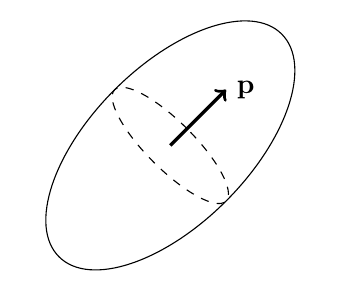
\begin{tikzpicture}[rotate=45]
        \draw(0,0) ellipse (2 cm and 1 cm);
        \draw[dashed](0,0) ellipse (0.3 cm and 1 cm);
        \draw[->,very thick](0,0) --++ (1,0)node[right]{$\textbf{p}$};
    \end{tikzpicture}
    \hfill
    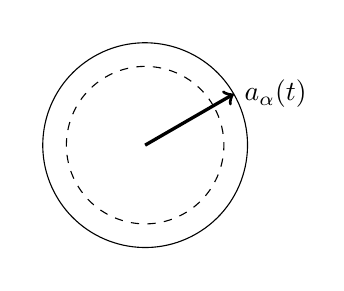
\begin{tikzpicture}[rotate=30]
        \draw(0,0) ellipse (1.3 cm and 1.3 cm);
        \draw[dashed](0,0) ellipse (1 cm and 1 cm);
        \draw[->,very thick](0,0) --++ (1.3,0)node[right]{$a_\alpha(t)$};
    \end{tikzpicture}
    \hfill
    \caption{Scheme of an axis symmetric particle with fore after symmetry and orientation normal vector \textbf{p}.}
    \label{fig:scheme2}
\end{figure}

\subsubsection*{Closures}
Initially we aim to solve the momentum equation for the fluid and particle phase \ref{eq:hybrid_avg_dt_rhou} and \ref{eq:hybrid_avg_dt_dp_alpha}. 
As previously mentioned these equations contain the following closures terms : $\oneavg{\textbf{T}}, \pnnavg{\textbf{f}_\alpha}, \pnnavg{\textbf{t}_\alpha}$ and $\pnnavg{\textbf{S}_\alpha}$ if we discard the fluctuation terms.
The closure for the averaged stress tensor appearing in \ref{eq:hybrid_avg_dt_rhou} can be express assuming solid unreformable motion inside the particles, with, \citep{jackson1997locally},



Note that the bulk velocity appearing in the above expression is in fact, $\avg{\textbf{u}} = \phi_1\oneavg{u} + \pnavg{\textbf{u}_\alpha} + \div (\pnavg{\mathcal{P}_\alpha})$.
Thus, the moment of momentum appear explicitly in the closure of the stress in agreement with \citet{zhang1997momentum}.  
Regarding the drag force, in  \citet{brenner1963resistance} they demonstrate that in low but finite inertia for an arbitrary shaped particle it could be expressed as,
\begin{equation}
    \textbf{f}_\alpha = 3 \pi \mu L \left[
        \textbf{R}_\alpha \cdot \textbf{U}
        + \frac{3}{16} Re  \left(
            3 \textbf{R}_\alpha 
            - \textbf{I} (\textbf{R}_\alpha : \textbf{e} \textbf{e})
        \right)
        \textbf{R}_\alpha\cdot  \textbf{U}
    \right]
\end{equation}
\JL{je pense pas que ce soit utile de citer Brenner \& Cox. On peut se limiter au regime de Stokes et juste dire que $\textbf{R}_\alpha$ depend de $\textbf{pp}$}
where $\textbf{U} = \oneavg{\textbf{u}}(\textbf{x}_\alpha)  - \textbf{u}_\alpha$ , $\textbf{e} = \textbf{U}/|\textbf{U}|$. 
and,  $\textbf{R}_\alpha$ is the resistance tensor in the laboratory frame. 
Besides, for axisymmetric particles with orientation vector \textbf{p} (sse \ref{fig:scheme2}) it can be shown that $\textbf{R}_\alpha = (R_{||} - R_\bot) \textbf{pp} + R_\bot \textbf{I}$, where $R_{||}$, $R_\bot$ are scalar coefficients \citep{guazzelli2011,kim2013microhydrodynamics}. 
Regarding the hydrodynamic torque applied on an asymmetric particle it can be expressed in Stokes regime as, 
\begin{equation}
    \textbf{t}_\alpha 
    = 
    \textbf{R}_{\omega T}\cdot \mathbf{\Omega}
     + \textbf{R}_{TU} \cdot \textbf{U} 
\end{equation}
where the first term represent the torque acting on the particle due to its translation,
with $R_T$ a correlation also function of the shape and $\textbf{U}$.
It must be noted that this relation remain partially true in low but finite inertial regime. 
Note that the correlation,  $R_T, R_{||} , R_{\bot}$ can be found in \citet{fintzi2023inertial} for cylindrical particles in dilute regime. 
And the second term represent the torque due to its rotation vector $\omega_\alpha$, where $\textbf{R}_{\omega T}$ is the resistance tensor linking rotation and torque \citet{pierson2021hydrodynamic} for inertial regime.  
Both $\textbf{R}_{\omega T}$ and $\textbf{R}_{TU}$ terms are function of the orientation of the particle \textbf{p}.
Closure for $\textbf{S}_\alpha$ can also be found but in the stokes regime only, 
indeed theoretical results are given in \citet[p 62]{kim2013microhydrodynamics}. Nevertheless, we do not provide them here as the expression is rather complicated. 
From the view of these closure terms we can see that in addition to the zeroth order terms, it is primordial to determine quantitatively the tensor $\textbf{pp}$, the rate of rotation $\omega_\alpha$ and the moment of momentum $\mathcal{P}_\alpha$. 

\subsubsection*{Dipole equations}
\JL{pourquoi dipole equations et pas first order moment equations ? l'expression dipole est utilise en mecanique des fluides mais pour des ecoulements potentiels generalement.}
Let consider a solid axis symmetric particle with fore after symmetric such that exposed in \ref{fig:scheme2}. 
Due to axis symmetric nature of the particle we can stipulate that, 
\begin{equation}
    \mathcal{M}_\alpha =  \textbf{pp} (M_\alpha^{||} - M_\alpha^\bot) 
    +  \textbf{I} M_\alpha^\bot
    \label{eq:M_definition}
\end{equation}
with $M_\alpha^{||}$, $M_\alpha^\bot$ being constant values related to the volume and shape of the particle. 
Besides, the velocity fields in inside each particle's domain can be deduced from solid body assumption, $\textbf{u}_2(\textbf{x}_\alpha + \textbf{r},t) = \textbf{u}_\alpha + \omega_\alpha \times \textbf{r}$ where $\omega_\alpha$ is the rotation vector of the particle $\alpha$.
By making use of this velocity decomposition it is easy to show that,
\begin{align}
    \mathcal{P}_\alpha
    &=  \omega_\alpha \times \left[
        \textbf{pp}(M_\alpha^{||} - M_\alpha^\bot) 
        + \textbf{I} M_\alpha^\bot
    \right]
    \label{eq:P_edfinition}\\
    2\mathcal{S}_\alpha
    &=  (M_\alpha^{||} - M_\alpha^\bot) \left(
        \omega_\alpha \times
        \textbf{pp}
        + \textbf{pp} \times \omega_\alpha
    \right)
    \label{eq:S_definition}\\
    \mu_\alpha / 
    &= \omega_\alpha \cdot \left[
        \textbf{pp} 
    (M_\alpha^{||}  - M_\alpha^{\bot} ) 
    - \textbf{I}(M_\alpha^{||} + M_\alpha^{\bot})
    \right]
    = \omega_\alpha \cdot\mathcal{I}_\alpha
    \label{eq:mu_definition}
\end{align}
Remark that  using the definition of $\mathcal{I}_\alpha$ yields a much simpler expression for $\mu_\alpha$. 

It is then straightforward to show that from \ref{eq:hybrid_avg_dt_dM_alpha},\ref{eq:S_definition} and \ref{eq:M_definition} we obtain the second order moment of volume conservation,
\begin{equation}
    \pddt (\pnavg{\textbf{pp}})
    + \div (
        \pnavg{\textbf{pp}\textbf{u}_\alpha}
        )
    = 
    \pnavg{\textbf{pp} \times \omega_\alpha}
    + \pnavg{\omega_\alpha \times \textbf{pp}} 
    % + \pnavg{\textbf{pp}' \times \omega_\alpha'}
    % +\pnavg{\omega_\alpha' \times \textbf{pp}'}
    \label{eq:hybrid_avg_dt_pp}
\end{equation}
In stokes flow we can find closure in the hypothesis of torque free particle, see \citet{kim2013microhydrodynamics}
\begin{equation}
    \omega_\alpha \times \textbf{p} 
    = -  \textbf{p} \times \omega_\alpha 
    = \avg{\Omega} \cdot \textbf{p} + \xi(\avg{\textbf{E}} \cdot \textbf{p} - \avg{\textbf{E}} \cdot \textbf{ppp})
    \label{eq:stokes_closure}
\end{equation}
Here $\avg{\textbf{E}}$ and $\avg{\Omega}$ are the symmetric and antisymmetric part of the velocity gradient. 
Injecting \ref{eq:stokes_closure} into \ref{eq:hybrid_avg_dt_pp} directly gives,
\begin{multline}
    \pddt (\pnavg{\textbf{pp}})
    + \div (
        \pnavg{\textbf{pp}\textbf{u}_\alpha}
        )
    = 
    \avg{\Omega} \cdot \pnavg{\textbf{pp}} 
    - \pnavg{\textbf{pp}} \cdot \avg{\Omega} \\
    + \beta\left[
        \avg{\textbf{E}} \cdot \pnavg{\textbf{pp}} 
        -\pnavg{\textbf{pp}} \cdot \avg{\textbf{E}} 
    - \avg{\textbf{E}} : \avg{\textbf{pppp}}
    \right]
    % \label{eq:hybrid_avg_dt_pp}
\end{multline}

In agreement with \citet{advani1987use} which found similar results except that they brought empirical expression for the fluctuation terms. \JL{je ne vois pas bien ou tu trouves cette equation dans le papier de Advani et Tucker ? D'ailleurs as tu lu Wang et Tucker 2008. Il est a mon avis plus explicite sur ce genre de chose.}

An equation for the rotation rate $\pnnavg{\omega_\alpha}$ can be obtained by, manipulating the angular momentum balance  \ref{eq:hybrid_avg_dt_dmu_alpha}, and using \ref{eq:mu_definition} and \ref{eq:hybrid_avg_dt_pp}, which gives,
\begin{multline}
    \left(
        \pnnavg{\textbf{pp}} 
        - \textbf{I}\frac{M_\alpha^{||} + M_\alpha^\bot}{M_\alpha^{||} - M_\alpha^\bot}
    \right)\left[
        \pddt (\pnavg{\omega_\alpha})
        + \div (
            \pnavg{\omega_\alpha}\pnnavg{\textbf{u}_\alpha}
            + \pnavg{\omega_\alpha'\textbf{u}_\alpha'})
        \right]\\
    +  \pnavg{\omega_\alpha}
    \cdot(\pnnavg{\omega_\alpha} 
    \times \pnnavg{\textbf{pp}})
    = \frac{\pnavg{\textbf{t}_\alpha}}{\rho_2}
    -\pnavg{\omega_\alpha' \cdot (\omega_\alpha \times \textbf{pp})'}
    +\pnavg{\omega_\alpha' \times \textbf{pp}}
    - \pnavg{\textbf{pp}'\dot{ \omega_\alpha}'}
\end{multline}
On the RHS we can observe that there is numerous closure fluctuation terms.  
\tb{FIND ref of this equations}\JL{as tu compare cette equation a celle de Zhang et Prosperreti 1997 ? }
\tb{they make spherical particle only so it is not interesting }
\subsubsection*{Stress equation}

Lastly, once we solved for $\pnnavg{\textbf{pp}}$ and $\pnavg{\omega_\alpha}$ we can deduce $\mathcal{S}_\alpha$ thanks to \ref{eq:S_definition}.
Afterward, we compute the integral of the undefined internal stress with \ref{eq:hybrid_avg_dt_dS_alpha}, which yield in our case, 
\begin{multline}
    \pnavg{\int_{\Omega_\alpha} 
        \mathbf{T}_2
    d\Omega}
    =  
      \pnavg{\textbf{S}_\alpha}
    - \rho_2\pnavg{\ddt \mathcal{S}_\alpha}\\
    - (M_\alpha^{||} - M_\alpha^\bot) \pnavg{
        (\omega_\alpha \times \textbf{p}) (\omega_\alpha \times \textbf{p}) } 
    -M_\alpha^\bot \pnavg{\textbf{I} \omega_\alpha^2 -\omega_\alpha\omega_\alpha }
    \label{eq:T2_definition}
\end{multline}
Then considering the particle nature it is possible to deduce its mean deformation from the stress integral, and validate or not the irreformability hypothesis made at start. 
It is also possible to compute the trace of the stress using \ref{eq:hybrid_avg_dt_dD_alpha}, yielding in this case, 
\begin{equation}
    \pnnavg{\int_{\Omega_\alpha} 
        \textbf{I}:\mathbf{T}_2
    d\Omega}
    =  
     (M_\alpha^{||} + M_\alpha^\bot) \pnnavg{
    \omega_\alpha^2} 
    - (M_\alpha^{||} - M_\alpha^\bot) \pnnavg{
    \omega_\alpha\omega_\alpha :  \textbf{pp}}
    + \pnnavg{\textbf{M}_\alpha} : \textbf{I}
\end{equation}
where we considered that the volume of the particle remained constant. 
This equation means that the rotational acceleration contribute to the isotropic particle pressure. 


In a pure rigorous manner the equivalent bulk stress of the suspension yield, 
\begin{equation*}
    \avg{\textbf{T}} = 
    \phi_1 \oneavg{\textbf{T}} 
    + \pnavg{\int_{\Omega_\alpha} \mathbf{T}_2 d\Omega}
    -\div \pnavg{\int_{\Omega_\alpha} \textbf{r}\mathbf{T}_2 d\Omega}
    + \ldots
\end{equation*}
Where the first and second terms on the RHS are given by \ref{eq:T_definition} and \ref{eq:T2_definition}, and the last one can be obtained with the third order moment of momentum equations. 
Anyhow, if we neglect this last term and if the solid motion hypothesis remain true we can determine the bulk stress using \ref{eq:T2_definition} which gives,
\begin{multline*}
    \avg{\textbf{T}} = 
    - \phi_1\oneavg{p}\textbf{I} 
    + \mu_1 \avg{\textbf{E}} 
    + \frac{1}{2}\frac{\pnavg{\textbf{S}_\alpha}}{\rho_2}
    - (M_\alpha^{||} - M_\alpha^\bot) \pnavg{\ddt \left(
        \omega_\alpha \times
        \textbf{pp}
        + \textbf{pp} \times \omega_\alpha
    \right)}\\
    - (M_\alpha^{||} - M_\alpha^\bot) \pnavg{
        (\omega_\alpha \times \textbf{p}) (\omega_\alpha \times \textbf{p}) } 
    -M_\alpha^\bot \pnavg{\textbf{I} \omega_\alpha^2 -\omega_\alpha\omega_\alpha }
\end{multline*}
\todo[inline]{Include an order and show the self torque part}
Each term on the RHS can be for one part factorized by \textbf{I} yieldings the equivalent pressure of the suspension, and an other part by $\avg{\textbf{E}}$ yielding the equivalent viscosity. 



\tb{
\subsubsection*{Oblate bubbles}

As it has already mentioned the trace of the moment of momentum equation can be used to derive the Reyl
It is also possible to derive from the second moment of mass equation an equation for the mean aspect ratio $\pnnavg{\xi}$ of the particles.
Indeed, let's consider obalte particles, such as droplets or bubble, in this case the second moment of mass can be written, $\mathcal{M}_\alpha =  \textbf{pp} [M_\alpha^{||}(t) - M_\alpha^\bot(t)] +  \textbf{I} M_\alpha^\bot(t)$
\tb{As in tomiyama example they state that the shape of the particle is of particular importance here the moment of volume matter }


\subsubsection*{Spherical compressible bubbles}
As mentioned in the \ref{sec:Lagrangian} from teh trace of the moment of momentum equation we can recover the Rayleigh-Lamb-Plesset equation.
Thus, by using the averaged moment of momentum equation we can falll back on \citet{zhang1994ensemble} model.

\subsubsection*{Slightly deformable elastic particle}

Now let consider the momentum conservation of slightly deformable particles.
First, the velocity field inside the particles, is assumed linear and incompressible, such that $\textbf{u}(\textbf{y}_\alpha) = \textbf{u}_\alpha + \mathcal{L}_\alpha \cdot \textbf{r}$ where the second order tensor  $\mathcal{L}_\alpha= \textbf{e}_\alpha+ \boldsymbol{\omega}$, with $\textbf{e}$ and $\boldsymbol{\omega}$ are symmetric and skew-symmetric tensors, respectively.
It directly follows from the expression of the velocity : $\mathcal{P}_\alpha = \int_{\Omega_\alpha} \textbf{r}\textbf{u} d\Omega = \mathcal{L}_\alpha\cdot \mathcal{M}$

The constitutive equation of the stress, $\textbf{T}_2$, within the particle phase can be written such as $\textbf{T}_2 = \mathbb{C} : \textbf{e}_2$ for elastic materials, with $\mathbb{C}$ the fourth order stiffness tensor and $ \textbf{e}_2 = \frac{1}{2}\left(\grad\textbf{u}_2+(\grad\textbf{u}_2)^T\right)$ is the rate of strain symmetric tensor.
Making use of the internal velocity expression yield directly the relation, $\textbf{e}_2=\textbf{e}_\alpha\cdot$ in $\Omega_\alpha$.

We know that the deformation of the particles will not have an explicit impact on the linear conservation equations.
Thus, we will be interested into the first and second order momentum and mass conservation equations respectively.
Making use of the average of \ref{eq:dt_P_alpha} over every configuration of the flow, and using the previous properties yield an equation for the average stress tensor within the suspension, namely,
\begin{equation}
    \pnnavg{\int_{\Omega_\alpha}\textbf{T}_\alpha d\Omega}
    = n_p\mathbb{C} : \pnnavg{(\mathcal{L}_\alpha+ \mathcal{L}_\alpha^T) v_\alpha}
    % = - \mathcal{L}_\alpha\cdot \mathcal{L}_\alpha\cdot \mathcal{M}_\alpha
    % - \mathcal{M}_\alpha \cdot\ddt \mathcal{L}_\alpha
    % - \textbf{M}_\alpha
    \label{eq:hybrid_avg_dt_P_alpha}
\end{equation}
\begin{equation}
    \mathcal{M}_\alpha \cdot\ddt \mathcal{L}_\alpha
    = - \mathcal{L}_\alpha\cdot \mathcal{L}_\alpha\cdot \mathcal{M}_\alpha
    - \mathbb{C} : (\mathcal{L}_\alpha+ \mathcal{L}_\alpha^T) v_\alpha
    - \textbf{M}_\alpha
    \label{eq:hybrid_avg_dt_P_alpha}
\end{equation}
Besed on that kind of argument \citet{lhuillier1987phenomenology}
}


One last remark is in order. 
With \ref{eq:dt_S_alpha} it is possible to compute the integral of the undefined internal stress $\int_{\Omega_\alpha} 
\mathbf{T}_2
d\Omega$ within the particle phase.
But first,  for a prolate spheroid the $\textbf{S}_\alpha$ may be written with this quite lenthly expression : 
\begin{multline}
    \textbf{S}_\alpha 
    = \frac{20}{3}\pi \mu a^3 \left[
    \left(
        X^M \mathbf{p}^{(0)}+Y^M \mathbf{p}^{(1)}+Z^M \mathbf{p}^{(2)}
    \right) : \textbf{E}\right.\\ \left.
    + \frac{3}{5} Y^H ((\mathbf{\Omega} - \omega_\alpha) \times \textbf{pp} + \textbf{pp} \times (\mathbf{\Omega} - \omega_\alpha) )
    \right]
    \label{eq:S_def}
\end{multline}
where, $X^M$, $Y^M$,  $Z^M$ and $Y^H$ are scalar resistance function related to the shape of the particles, and the $\mathbf{p}^{(i)}$ are fourth order orientation tensor solely express in terms of $\textbf{p}$, all of which are given in \citet[p 62.]{kim2013microhydrodynamics}. 
theerfore, by rearranging the term for the integrated stress, \ref{eq:dt_S_alpha}, can be written for axissymmetric particles such as, 
\begin{multline}
    \pnavg{\int_{\Omega_\alpha} 
        \mathbf{T}_2
    d\Omega}
    =  
      \pnavg{\textbf{S}_\alpha}
    - (M_\alpha^{||} - M_\alpha^\bot)\pnavg{\ddt  \left(
        \omega_\alpha \times
        \textbf{pp}
        + \textbf{pp} \times \omega_\alpha
    \right) }\\
    - (M_\alpha^{||} - M_\alpha^\bot) \pnavg{
        (\omega_\alpha \times \textbf{p}) (\omega_\alpha \times \textbf{p}) } 
    -M_\alpha^\bot \pnavg{\textbf{I} \omega_\alpha^2 -\omega_\alpha\omega_\alpha }
\end{multline}
which is a constitutive expression of the stress. 
In stokes flow condition one may argue that all product of $\omega_\alpha$ and time derivative of $\omega$ are negligible, leavening with the stresslet. 
% \section{The equivalent stresses of an emulsion}

We consider a multiphase flow with no-mass transfer, i.e. $\textbf{u}_k=\textbf{u}_I$.
The interfaces have negligible weight and no interfacial viscosity. 

\subsection{Momentum equation}
The  continuous and particle averaged momentum equation of the continuous and dispersed phase now reads as, 
\begin{align*}
    \pddt (\rho_1\phi_1 \textbf{u}_1 )
    + \div (\rho_1\phi_1 \textbf{u}_1  \textbf{u}_1
    + \bm{\sigma}^\text{eff}_1 
    - \phi_1 \bm{\sigma}_1)
    &= 
    \phi_1 \textbf{b}_1
    - n_p \textbf{f}_p \\
    \pddt (n_p m_p \textbf{u}_p)
    + \div (
        n_p m_p \textbf{u}_p\textbf{u}_p
        + \bm{\sigma}^\text{eff}_p
        )
    &= 
     n_p v_p 
      \textbf{b}_2
    + n_p \textbf{f}_p ,
\end{align*}
Alternatively, they can be written as :
\begin{align*}
    \pddt (\rho_1\phi_1 \textbf{u}_1 )
    + \div (\rho_1\phi_1 \textbf{u}_1  \textbf{u}_1
    + \bm{\sigma}^\text{eff}_1 )
    &= 
    \phi_1( \textbf{b}_1  +\div  \bm{\sigma}_1)
    - n_p \textbf{f}_p \\
    \pddt (n_p m_p \textbf{u}_p)
    + \div (
        n_p m_p \textbf{u}_p\textbf{u}_p
        + \bm{\sigma}^\text{eff}_p
        )
    &= 
     n_p v_p (
      \textbf{b}_2
    + \div \bm{\sigma}_1 )
    + n_p \textbf{f}_p ,
\end{align*}
With the following definition, 
\begin{align*}
    \bm{\sigma}^\text{eff}_1
    &=\rho_1 \phi_1 \oneavg{\textbf{u}_1'\textbf{u}_1'}
    - n_p \textbf{M}_p 
    \\
    \bm{\sigma}^\text{eff}_2
    &= m_p \pnavg{ \textbf{u}_\alpha'\textbf{u}_\alpha'} 
\end{align*}
With the exchange terms function of teh relative or local stress $\bm{\sigma}_1'=\bm{\sigma}_1^0 - \bm{\sigma}_1$. 

Now we start by deriving each stress considering Newtonian fluid for the dispersed phase. 
\begin{align*}
    \bm{\sigma}_1 
    &= - p_1 \textbf{I}
    + \frac{\mu_1 }{\phi_1} \textbf{e}
    - \frac{\lambda \mu_2 \phi_2}{\phi_1} \textbf{e}_2\\
    \bm{\sigma}_1 
    &= - \left(p_1 + \frac{\lambda }{\phi_1}\phi_2 p_2\right) \textbf{I}
    + \frac{\mu_1}{\phi_1} \textbf{e}
    - \frac{\lambda }{\phi_1} \phi_2 \bm{\sigma}_2 \\
    \phi_1 \bm{\sigma}_1 
    &= - (\phi_1 p_1+ \lambda \phi_2 p_2) \textbf{I}
    + \mu_1 \textbf{e}
    - \lambda \phi_2 \bm{\sigma}_2\\
\end{align*}
Injecting this last equation onto the fluid phase formula gives, 
\begin{align*}
    \pddt (\rho_1\phi_1 \textbf{u}_1 )
    + \div (\rho_1\phi_1 \textbf{u}_1  \textbf{u}_1
    + \bm{\sigma}^\text{Re}_1 
    + \phi_1 p_1 \textbf{I}
    - \mu_1 \textbf{e}
    + \lambda \phi_2 \mu_2 \bm{e}_2)
    &= 
    \phi_1 \textbf{b}_1
    - \avg{\delta_I \bm{\sigma}_1 \cdot \textbf{n}_2} \\
\end{align*}
We can substitue the particle phase stress with it's respective momentum equation,
\begin{equation*}    
\div (\phi_2 \mu_2 \bm{e}_2)
=  
\grad (\phi_2 p_2 \textbf{I})
-\pddt (\phi_2\rho_2 \textbf{u}_2)
- \div (\phi_2\rho_2 \textbf{u}_2 \textbf{u}_2)
- \phi_2 \textbf{b}_2 
- \avg{\delta_I
    \bm{\sigma}_1^0
\cdot \textbf{n}_2}
- \div (\phi_I \bm{\sigma}_I) ,
\end{equation*}
Which gives, 
\begin{multline*}
    \pddt (\rho_1\phi_1 \textbf{u}_1 -\lambda \phi_2 \rho_2 \textbf{u}_2  )
    + \div (
        \rho_1\phi_1 \textbf{u}_1  \textbf{u}_1
        - \lambda\rho_2\phi_2 \textbf{u}_2  \textbf{u}_2
    + \bm{\sigma}^\text{Re}_1 - \lambda \bm{\sigma}^\text{Re}_2 \\
    + (\phi_1 p_1 + \phi_2 \lambda p_2) \textbf{I}
    - \mu_1 \textbf{e})
    = 
    \phi_1  \textbf{b}_1
    + \lambda \phi_2  \textbf{b}_2
    - (1-\lambda)\avg{\delta_I \bm{\sigma}_1 \cdot \textbf{n}_2}
    + \div (\phi_I \bm{\sigma}_I) \\
\end{multline*}


A more easy way to model these,
\begin{multline}
    \int_{\Omega_\alpha} 
    (\bm{\sigma}_2^0)_{ik}
    d\Omega
    = 
    - \int_{\Sigma_\alpha} 
    (\bm{\sigma}_I)_{ik}
    d\Sigma
    +  \int_{\Omega_\alpha} \rho_2 
    (\textbf{w}_2^0\textbf{w}_2^0  )_{ik}
    d\Omega
    -\ddt \int_{\Omega_\alpha} r_i (\textbf{u}^0_2)_k \Omega
    +\int_{\Sigma_\alpha} 
     r_i (\bm{\sigma}_1^0 \cdot \textbf{n}_2)_{k}
    d\Sigma
\end{multline}
Besides using the general formula \ref{eq:dt_Q_n} for $n = 2$ we obtained the relation, 
\begin{multline}
    \int_{\Omega_\alpha} (r_{j}(\bm{\sigma}^0_2)_{ki}+r_{k}(\bm{\sigma}^0_2)_{ji})d\Omega
    +\int_{\Sigma_\alpha} (r_{j}(\bm{\sigma}^0_I)_{ki}+r_{k}(\bm{\sigma}_I^0)_{ji})d\Sigma
    = \\
    - \ddt\int_{\Omega_\alpha} \rho_2 (\textbf{u}_2^0)_i r_j r_k d\Omega
    + \int_{\Omega_\alpha} \rho_2 (r_{j} (\textbf{w}_2^0)_k (\textbf{u}^0_2)_i + r_k (\textbf{w}_2^0)_j (\textbf{u}^0_2)_i)d\Omega\\
    +\int_{\Sigma_\alpha}  r_{k}r_{j} (\bm{\sigma}_1^0)_{il} (\textbf{n}_2)_l d\Sigma
    + \int_{\Omega_\alpha} r_{k}r_{j}  \rho_2 d\Omega g_i
\end{multline}
% \section{Examples and applications}




\section{Discussion and conclusion}
\begin{itemize}
\item We clarified the momentum stress components for dorps
\begin{itemize}
    \item The extra deformation tensor is acctually part of the stresslet definition.
\end{itemize}
\item The energy equaiton is derived for fluid particle
\begin{itemize}
    \item We make appear the source terms clearly.
    \item We distinguish the differents contributions. 
\end{itemize}
\item Special application to Hill vortecies
\item Mention of other applications
\end{itemize}
\section{Discussion and conclusion}

In this chapter, many advances have been made regarding the modeling of dilute emulsion of slightly deformable droplets. 
We summarize these advancements in three main points which are as follows: 
\begin{enumerate}
    \item We have shown in the first place how, from the first moment of momentum and second moment of mass equation we could derive tensor equations for the particle mean shear rate and deformation tensor. 
In addition to the classic equation of deformation, already obtained in \citet{goddard1967nonlinear},  and the angular momentum equation, it has been shown that the symmetric part of the moment of momentum equation corresponds to the second oscillatory mode equation of the droplets. 
More specifically, we derived this equation while staying general on the droplet's internal motion, making the forcing term of this oscillatory equation explicit in terms of the local properties of the particles and carrier fluid. 
Although not closed these forcing terms exhibit more physical sense than the usually undefined forcing term used in the classic second-order oscillatory model.
For example, in \citet{riviere2021sub} they use such a forcing term, but it is not directly related to the fluid and particle locals properties.
However, with our formalism, we were able to express explicitly what are the forcing terms of this equation, although not closed. 

\item 
The second advancement of this chapter is the proposition of solving for the eigenvalues of the deformation and rate of deformation and angular rotation vector of the particle, instead of directly solving for the corresponding quantities in the laboratory reference frame. 
In this way, we demonstrate that we reduce drastically the number of equations due to the limited degrees of freedom considered for the deformation of the drops. 
These Lagrangian equations are then averaged. 
We then discover the counterpart of solving for the eigenvalues of the mentioned tensors; 
Indeed, at the cross-grained level, we solve for the average of these eigenvalues. 
However, we now need new closure to determine the average of the corresponding tensor in the laboratory reference frame.  
This calls into question the efficiency of this local basis formulation since the expression of some of these tensors, especially the angular rotation vector is indispensable in some situations. 

\item Finally,  in the motivation of improving the modeling 1D Navier-Stokes averaged equations we end this work with an analysis of the phases relative motion on the particle deformation and carrier fluid phase stress. 
In the first place, we could demonstrate an alternative derivation of the droplet's deformation generated by relative translation at finite Reynolds number, as in the study of \citet{taylor1964deformation}. 
Our methodology is based on the averaged particle equations derived in the previous section and explicit closures are derived using an extended Reciprocal Theorem suited for spherical droplets. 
With the aid of DNS we could validate the theoretical result in the low but finite inertial regime. 
Lastly, we discuss the impact of particle translation on the suspension stress. 
It is shown that the exchange terms responsible for the droplets' deformation, i.e. the \textit{Stresslet} term, were also responsible for an additional source in the continuous phase stress. 
Notably, we could show that the \textit{Stresslet} term usually neglected in this context is not null and is function of the particle-carrier phase relative velocity square and $\phi Re$.  
When considering only relative translation this term is in competition with the \textit{Reynolds stress} term, which is shown to be comparable to the \textit{Stresslet} term. 
As the Reynolds stress term is shown to be $\sim \phi^{2/3}$ while the \textit{Stresslet} is $\sim \phi$ we might expect the latter negligible in the dilute regime but dominant in the dense regime. 
At $\phi = 0.05$ we state that the contribution of the \textit{Stresslet} is about 10\% of the \textit{Reynolds stress} contribution. 
The \textit{Stresslet} term might eventually be more important than the \textit{Reynolds stress} term if the droplets possess a higher density ratio. 
\end{enumerate}


\section*{Acknowledgement}
We would like to express our sincere gratitude to Professor D. Lhuillier for his inspiring and insightful class, which has greatly influenced our work.
Also, the authors are grateful for many in-depth discussions with Professor St\'ephane Popinet from \textit{Institut Jean le Rond Alembert} as well. 
\bibliography{Bib/bib_bulles.bib}



\appendix

% \section{Singularity solution}

In this appendix we consider the calculation of the zeroth and second moment of force density around a spherical droplet translating with a relative velocity \textbf{U} in the carrier fluid and having a viscosity ratio $\lambda$. 
In \citet{kim2013microhydrodynamics,pozrikidis1992boundary} the velocity \textbf{u},$\hat{\textbf{u}}$ and pressure fields $p$,$\hat{p}$ inside and outside (denoted by a hat ) is given in the form, 
\begin{align*}
    u_i(\textbf{r})
    = G_{ij}(\textbf{r}) g_j 
    + D_{ij}(\textbf{r}) d_j 
    &\;\;\; p(\textbf{r})
    = 2 \mu \frac{x_j}{r^3}g_j
    & \sigma_{ij}^0 
    = \mu_1 ( T^G_{ijk} g_j + T^D_{ijk} d_j )\\
    \hat{u}_i(\textbf{r})
    = c_i 
    + E_{ij}(\textbf{r}) e_j 
    &\;\;\;\hat{p}(\textbf{r})
    = 10 \mu r_je_j
    & \hat\sigma_{ij}^0 
    = \mu_2 T^E_{ijk} e_j 
\end{align*}
Where the constant are defined such that,
\begin{align*}
    &\textbf{g} = \frac{1}{4}\left(\frac{3\lambda + 2}{\lambda +1}\right) a \textbf{U}
    &\textbf{d} = -\frac{1}{4}\left(\frac{\lambda}{\lambda +1}\right) a^3 \textbf{U}\\
    &\textbf{c} = \frac{1}{2}\left(\frac{3\lambda + 3}{\lambda +1}\right) \textbf{U}
    &\textbf{e} = -\frac{1}{2}\left(\frac{1}{\lambda +1}\right) \frac{1}{a^2} \textbf{U}\\
\end{align*}
And the functions follow decaying harmonics functions \textbf{G}(\textbf{r}) and \textbf{D}(\textbf{r}) reads, 
\begin{align*}
    G_{ij}(\textbf{r})
    = \frac{\delta_{ij}}{r}
    + \frac{r_ir_j}{r^3}
    && T^G_{ijk}
    = - 6 \frac{r_ir_jr_k}{r^5}\\
    D_{ij}(\textbf{r})
    = -\frac{\delta_{ij}}{r^3}
    + 3 \frac{r_ir_j}{r^5}
    &&
    T^D_{ijk}
    = 6\frac{\delta_{ij}r_k+\delta_{ik}r_j + \delta_{jk}r_i}{r^5}
    -30 \frac{r_ir_jr_k}{r^7}
\end{align*}
Lastly the growing harmonics \textbf{E}(\textbf{r}) reads, 
\begin{align*}
    E_{ij}(\textbf{r})
    = 2 r^2 \delta_{ij}
    - r_ir_j. 
    &&
    T^E_{ijk}(\textbf{r})
    = 3(-4\delta_{ik} r_j + \delta_{ij}x_k + \delta_{kj}x_i )
\end{align*}


The aim is now to compute the integrals of the form, 
\begin{align*}    
    \pMSavg{\textbf{r}\bm{\sigma}_1^0\cdot \textbf{n}_2}
    - \pMOavg{\mu_1 \textbf{e}_2 },
\end{align*}
in the case of a relative linear flow fields. 
Thus, one must compute the integrals, 
\begin{align*}
    \pSavg{\bm\sigma_1^0\cdot \textbf{n}_2}
    &&
    \pSavg{\textbf{rr}\bm\sigma_1^0\cdot \textbf{n}_2 - \mu_1 \textbf{r}\textbf{e}_2^0}
\end{align*}
Since the first order moment is identically zero. 
To do so we first recall that, 
\begin{equation}
    \bm\sigma_k^0
    = 
    - p_k \textbf{I}
    + \mu_1 \left(
        \frac{\partial u_{k,i}^0}{\partial x_j}
        + \frac{\partial u_{k,j}^0}{\partial x_i}
    \right)
\end{equation}
The exterior stress filed

\subsubsection*{The drag force}

% \section{Derivation of the point velocity}
\label{ap:velocity_definition}
In this Appendix we derive the velocity of the center of mass of a particle $\alpha$. Consider a particle of center of mass $\textbf{y}_\alpha$ defined such as
\begin{equation*}
    m_\alpha(t) \textbf{y}_\alpha(t)
    = \int_{\Omega_\alpha} \rho_2 \textbf{y}_2 d\Omega,
\end{equation*}
where we empathize that both, $m_\alpha(t)$ and $\textbf{y}_\alpha(t)$ are function of time. 
The center of mass velocity is defined as the derivative of $\textbf{y}_\alpha(t)$ within time.
Yielding, 
\begin{align*}
    \frac{d}{dt} \textbf{y}_\alpha (t)
    &=
    \frac{d}{dt} \left(
        \frac{1}{m_\alpha} \int_{\Omega_\alpha} \rho_2 \textbf{y}_2 d\Omega
    \right)\\
    &= \frac{1}{m_\alpha}
    \frac{d}{dt} 
    \left(
        \int_{\Omega_\alpha} \rho_2 \textbf{y} d\Omega
    \right)
    - \frac{1}{m_\alpha^2} \frac{d}{dt} \int_{\Omega_\alpha} \rho_2 d\Omega \int_{\Omega_\alpha} \rho_2 \textbf{y}_2 d\Omega
    \\
    &= \frac{1}{m_\alpha}\int_{\Omega_\alpha} \left[
        \pddt (\rho_2 \textbf{y}) + \div\left(\rho_2 \textbf{y}\textbf{u}_2\right) 
    \right]d\Omega \\
    &+ \frac{1}{m_\alpha}\int_{\Sigma_\alpha} \textbf{y} \rho_2(\textbf{u}_I   - \textbf{u}_2) \cdot \textbf{n}_2 d \Sigma
    -  \frac{1}{m_\alpha^2} \int_{\Sigma_\alpha} \rho_2(\textbf{u}_I   - \textbf{u}_2) \cdot \textbf{n}_2 d\Sigma  \int_{\Omega_\alpha} \rho_2 \textbf{y}_2 d\Omega
    \\
    &= \frac{1}{m_\alpha}\int_{\Omega_\alpha} \textbf{y} \left[
    \pddt (\rho_2) + \div\left(\rho_2 \textbf{u}_2\right) 
    \right]d\Omega
    + \frac{1}{m_\alpha}\int_{\Omega_\alpha} \rho_2  \textbf{u}_2  \cdot \grad \textbf{y} d\Omega \\
    &+ \frac{1}{m_\alpha}\int_{\Sigma_\alpha} \textbf{y}_2 \rho_2 (\textbf{u}_I - \textbf{u}_2) \cdot \textbf{n}_2 d \Sigma
    - \frac{1}{m_\alpha}  \textbf{y}_\alpha \int_{\Sigma_\alpha} \rho_2(\textbf{u}_I   - \textbf{u}_2) \cdot \textbf{n}_2 d\Sigma
\end{align*}
By considering the mass conservation on a single fluid particle for the first term, noticing that $\grad \textbf{y} = \textbf{I}$ where $\textbf{I}$ is the identity tensor for the second term, and introducing $\mathbf{r} = \mathbf{y} - \mathbf{y}_\alpha$ for the last two terms gives, 
\begin{equation*}
    \textbf{u}_\alpha
    = \frac{1}{m_\alpha} \left(
        \int_{\Omega_\alpha} \rho_2 \textbf{u}_2 d\Omega
        +  \int_{\Sigma_\alpha} \rho_2 \textbf{r}  (\textbf{u}_I - \textbf{u}_2) \cdot \textbf{n}_2 d\Sigma
    \right).
    \label{eq:vel_def}
\end{equation*}

\section{Leibniz and Gauss divergence theorem for volume and surface integral}
\label{ap:math}

In this appendix we recall the form of the Leibnitz rules, Gauss integral rule and general Reynolds transport theorem. 
\subsubsection*{Volume integral over $\Omega_\alpha$}
For a surface integral over a closed surface the Gauss divergence theorem reads : 
\begin{equation}
    \int_{\Sigma_\alpha} \textbf{f} \cdot \textbf{n}_2 d\Sigma
    = \int_{\Omega_\alpha} \div \textbf{f}d\Omega
\end{equation}

To differentiate time varying integral we make use of the Reynolds transport theorem.
For a quantity $\textbf{f}$ of arbitrary tensorial order, it is defined  as follows in our notation, 
% \begin{equation}
%     \frac{d}{dt} \int_{\Omega_\alpha} \textbf{f} d\Omega
%     = \int_{\Omega_\alpha}\pddt \textbf{f}  d\Omega
%     + \int_{\Sigma_\alpha} \textbf{f} \textbf{u}_I \cdot \textbf{n}_2 d\Sigma,
% \end{equation}
% then by adding and subtracting  $\int_{\Sigma_\alpha} \textbf{f} \textbf{u}_2 \cdot \textbf{n}_2 d\Sigma$ on the RHS we arrive to the more practical expression,
\begin{equation}
    \frac{d}{dt} \int_{\Omega_\alpha} \textbf{f} d\Omega
    = \int_{\Omega_\alpha}\left[\pddt \textbf{f} + \div\left(\textbf{f}\textbf{u}_2\right) \right]d\Omega\\
    + \int_{\Sigma_\alpha} \textbf{f} (\textbf{u}_I-\textbf{u}_2)\cdot \textbf{n}_2 d\Sigma,
    \label{eq:Reynolds}
\end{equation}


\subsubsection*{Surface integral over $\Sigma_\alpha$}

In this work we are solely interested in closed surface topology. 
For a clear demonstration of the Reynolds transport and divergence theorem for interfaces we refer the reader to the work of \citet{nadim1996concise}. 
For closed surface integral the Gauss divergence theorem reads as :
\begin{equation}
    \int_{\Sigma_\alpha}  \divI \textbf{f} d\Sigma
    = 
    \int_{\Sigma_\alpha}  \textbf{f} \cdot \textbf{n}\divI\textbf{n} d\Sigma. 
    \label{eq:surf_div_theorem}
\end{equation}
Note that only the normal component of $\textbf{f}$ remain meaning that the integral any tangential tensor $\textbf f_{||}$ vanish. 
Additional, The time derivative of any surface integral can then be obtained using Leibniz rule, which reads as  
\begin{equation}
    \frac{d}{dt} \int_{\Sigma_\alpha} \textbf{f} d\Sigma 
    = \int_{\Sigma_\alpha} \left[
        \pddt \textbf{f} 
        +   \divI (\textbf{u}_I\textbf{f})
    \right]d\Sigma,
    \label{eq:Leibnitz}
\end{equation}
The formulation of \ref{eq:Leibnitz} is sometime preferred as the partial time derivative exist only on the surface. 

\section{A detailed derivation of the moments conservation equaitons}
\label{ap:moment_derivative}
In this appendix we propose a detailed derivation of the moments equations. 
The first moment or dipoles of any property $q_\alpha$ can be defined as,
\begin{equation*}
    \mathcal{Q}_\alpha 
    = \int_{\Omega_\alpha} \textbf{r} f_2 d\Omega
\end{equation*}
We use the Reynolds transport theorem to describe the evolution of $\mathcal{Q}_\alpha$ within time. 
It gives, 
\begin{align*}
    \frac{d}{dt} \mathcal{Q}_\alpha
      &=  \int_{\Omega_\alpha} \left[
        \pddt(\textbf{r}  f_2)
        + \div \left(f \textbf{r} \textbf{u}_2\right)
    \right]d\Omega + \int_{\Sigma_\alpha} \textbf{r}  f_2  (\textbf{u}_I-\textbf{u}_2)\cdot \textbf{n}_2  d\Sigma  \nonumber \\
    &=  \int_{\Omega_\alpha} \textbf{r}\left[
        \pddt f_2
        + \div \left(f_2 \textbf{u}_2\right)
    \right] d\Omega
    + \int_{\Omega_\alpha} f_2 \left[
        \pddt \textbf{r}
        +\textbf{u}_2 \grad \textbf{r}
    \right]d\Omega\\
    &+ \int_{\Sigma_\alpha} \textbf{r}  f_2 (\textbf{u}_I-\textbf{u}_2)\cdot \textbf{n}_2  d\Sigma,
\end{align*}
Using \ref{eq:dt_f_k} for the first term, and considering the relation,
$  \pddt \textbf{r}
+ \textbf{u}_2 \cdot \grad \textbf{r}
= - \frac{d}{dt} \textbf{y}_\alpha  + \textbf{u}_2 \cdot \textbf{I}
= \textbf{w}_2$,
for the second yields the relation,
\begin{align*}
    \frac{d}{dt} \mathcal{Q}_\alpha
    &= \int_{\Omega_\alpha} \textbf{r} \left[
         \textbf{S}_2 +  \div \mathbf{\Phi}_2
    \right]d\Omega
    +\int_{\Omega_\alpha} f_2  \textbf{w}_2 d\Omega
    + \int_{\Sigma_\alpha} \textbf{r}  f_2 (\textbf{u}_I-\textbf{u}_2)\cdot \textbf{n}_2  d\Sigma,\\
    &= \int_{\Omega_\alpha} \left( 
        \textbf{r} \textbf{S}_2 
        - \mathbf{\Phi}_2
        + f_2  \textbf{w}_2 
    \right) d\Omega
    + \int_{\Sigma_\alpha} \textbf{r} \left[
        \mathbf{\Phi}_2
        + f_2 (\textbf{u}_I-\textbf{u}_2)
    \right]\cdot \textbf{n}_2  d\Sigma.
\end{align*}
To pass from the first line to the second lines we noticed that $\int_{\Omega_\alpha} \textbf{r}  \div \mathbf{\Phi}_2 d\Omega
= \int_{\Sigma_\alpha} \textbf{r} \mathbf{\Phi}_2 \cdot \textbf{n}_2 d\Sigma
- \int_{\Omega_\alpha} \mathbf{\Phi}_2 d\Omega$. 
% \JL{Dans le corps du texte tu notes $d\Sigma$ et $d\Omega$ les differentielles des surfaces et des volumes. Merci de faire la meme chose en annexe. Par ailleurs je trouve qu'il manque des explications pour passser de 78 a 79 (j'imagine que tu utilises la conservation du moment d'ordre 0) et pour passer de 79 a 80 ou tu dois faire une integration part partie. Encore faut il le preciser ...}


% 
\section{Arbitrary order moments equation}
\label{ap:Moments_equations}
In this appendix we extend the Lagrangian conservation laws to an arbitrary order moment equation. 
Let's define the arbitrary moment of the Eulerian field $f$, by, 
\begin{equation*}
    \mathcal{Q}_{i_1\ldots i_n}
    = \int_{\Omega_\alpha} 
    \pri{1}{n} f d\Omega
\end{equation*}
Then by using the Reynolds transport theorem we can equally show that :
\begin{multline*}
    \ddt {\mathcal{Q}_{i_1\ldots i_n}}
    =\int_{\Omega_\alpha} \left[ \partial_t \left(\pri{1}{n}f\right) 
    + \partial_k \left(u_k \pri{1}{n}f\right) \right]d\Omega\\
    +\int_{\Sigma_\alpha} \pri{1}{n} f \left(u^I_k - u_k\right) n_k d\Sigma.
\end{multline*}
Using the product rule on the first integral derivatives yields, 
\begin{multline*}
    \ddt {\mathcal{Q}_{i_1\ldots i_n}}
    =\int_{\Omega_\alpha} f \left[ \partial_t \left(\pri{1}{n}\right) 
    + u_k \partial_k \left( \pri{1}{n}\right) \right]d\Omega\\
    +\int_{\Omega_\alpha} \pri{1}{n} \left[ \partial_t \left(f\right) 
    +  \partial_k \left(u_k f \right) \right]d\Omega\\
    +\int_{\Sigma_\alpha} \pri{1}{n} f \left(u^I_k - u_k\right) n_k d\Sigma.
\end{multline*}
Proceeding with a similar manner than for the first moment conservation equation we can equally show that, 
\begin{multline*}
    \ddt {\mathcal{Q}_{i_1\ldots i_n}}
    = \sum_{e=1}^{n} \int_{\Omega_\alpha} f  \prod^{n}_{\substack{ m=1 \\   m \neq e}} r_{i_m} w_{i_e}d\Omega
    +\int_{\Omega_\alpha} \pri{1}{n} \div\mathbf{\Phi} d\Omega\\
    + \int_{\Omega_\alpha} \pri{1}{n} \textbf{S} d\Omega
    +\int_{\Sigma_\alpha} \pri{1}{n} f \left(u^I_k - u_k\right) n_k d\Sigma.
\end{multline*}
The second term of this equation can be written,
\begin{align*}
    \int_{\Omega_\alpha} \pri{1}{n} \div\mathbf{\Phi} d\Omega
    &= \int_{\Sigma_\alpha} \div \left(\pri{1}{n} \mathbf{\Phi} \right)d\Omega
    - \int_{\Omega_\alpha} \mathbf{\Phi} \cdot \grad \left(\pri{1}{n} \right)d\Omega\\
    &= \int_{\Sigma_\alpha} \pri{1}{n} \mathbf{\Phi} \cdot \textbf{n}d\Sigma
    -\sum_{e=1}^{n} \int_{\Omega_\alpha} \mathbf{\Phi}  \prod^{n}_{\substack{ m=1 \\m \neq e}} r_{i_m}  d\Omega
\end{align*}
Including this relation into the former equation yields, 
\begin{multline}
    \ddt {\mathcal{Q}_{i_1\ldots i_n}}
    = \sum_{e=1}^{n} \int_{\Omega_\alpha} \prod^{n}_{\substack{ m=1 \\   m \neq e}} r_{i_m} (w_{i_e}f  - \mathbf{\Phi}_{i_e})d\Omega
    +\int_{\Sigma_\alpha} \pri{1}{n} \mathbf{\Phi} \cdot \textbf{n}d\Sigma\\
    + \int_{\Omega_\alpha} \pri{1}{n} \textbf{S} d\Omega
    +\int_{\Sigma_\alpha} \pri{1}{n} f \left(u^I_k - u_k\right) n_k d\Sigma.
    \label{eq:dt_Q_n}
\end{multline}
For scalar quantity this expression is purely symmetric since it involve only product of the $r_{i_n}$ with scalar, and sum over all vector indexed by $i_e$
Let focus on the case were $f$ is a vector indexed $k$ we have, 
\begin{multline}
    \ddt {\mathcal{Q}_{i_0 i_1\ldots i_n }}
    = \sum_{e=1}^{n} \int_{\Omega_\alpha} \prod^{n}_{\substack{ m=1 \\   m \neq e}} r_{i_m} (w_{i_e}f_{i_0}  - \mathbf{\Phi}_{i_0 i_e})d\Omega
    +\int_{\Sigma_\alpha} \pri{1}{n} (\mathbf{\Phi} \cdot \textbf{n})_{i_0}d\Sigma
    + \int_{\Omega_\alpha} \pri{1}{n} \textbf{S}_{i_0} d\Omega
\end{multline}
The symmetric part of $\mathcal{Q}_{i_0 i_1\ldots i_n}$ is, 
\begin{equation*}
    \mathcal{Q}_{(i_0 i_1\ldots i_p \ldots i_n )}
= \frac{1}{n+1}
\sum_{p=0}^{n} \mathcal{Q}_{i_p (i_1\ldots i_0\ldots i_n)}
\end{equation*}
where the parenthesis indicates the symmetric index, and it must be understood that this is permutation of the indices.  
Therefore, the fully symmetric part of the preceding momentum balance can be obtained by summing every permutation of the index $k$ with all other index and dividing by $n$, namely,
\begin{multline}
    \ddt {\mathcal{Q}_{(i_0 i_1\ldots i_n) }}
    = \frac{1}{n+1}
    \sum_{p=0}^{n}
    \sum_{\substack{ e=0 \\   e \neq i_p}}^{n} \int_{\Omega_\alpha} 
    \prod^{n}_{\substack{ m=0 \\   m \neq e}} r_{i_m} (w_{i_e}f_{i_p}  - \mathbf{\Phi}_{i_p i_e})d\Omega\\
    +\frac{1}{n+1}
    \sum_{p=0}^{n}
    \int_{\Sigma_\alpha} \prod^{n}_{\substack{ m=0 \\   m \neq i_p}} r_{i_m}
    (\mathbf{\Phi} \cdot \textbf{n})_{i_p}d\Sigma
    + \int_{\Omega_\alpha} 
    \prod^{n}_{\substack{ m=0 \\   m \neq i_p}} r_{i_m}
    \textbf{S}_{i_p} d\Omega
\end{multline}
It appears that this equation is the fully symmetric parts of the moments equations. 
The skew symmetric parts will be written, 
\begin{multline}
    \frac{d}{dt} (
    \mathcal{Q}_{i_0 i_1\ldots i_n} 
    - \mathcal{Q}_{(i_0 i_1\ldots i_n) }
    )
    = 
    \sum_{e=1}^{n} \int_{\Omega_\alpha} \prod^{n}_{\substack{ m=1 \\   m \neq e}} r_{i_m} (w_{i_e}f_{i_0}  - \mathbf{\Phi}_{i_0 i_e})d\Omega
    -
    \frac{1}{n+1}
    \sum_{p=0}^{n}
    \sum_{\substack{ e=0 \\   e \neq i_p}}^{n} \int_{\Omega_\alpha} 
    \prod^{n}_{\substack{ m=0 \\   m \neq e}} r_{i_m} (w_{i_e}f_{i_p}  - \mathbf{\Phi}_{i_p i_e})d\Omega\\
    +\int_{\Sigma_\alpha} \pri{1}{n} (\mathbf{\Phi} \cdot \textbf{n})_{i_0}d\Sigma
    -
    \frac{1}{n+1}
    \sum_{p=0}^{n}
    \int_{\Sigma_\alpha} \prod^{n}_{\substack{ m=0 \\   m \neq i_p}} r_{i_m}
    (\mathbf{\Phi} \cdot \textbf{n})_{i_p}d\Sigma
    + \int_{\Omega_\alpha} \pri{1}{n} \textbf{S}_{i_0} d\Omega
    -
    \int_{\Omega_\alpha} 
    \prod^{n}_{\substack{ m=0 \\   m \neq i_p}} r_{i_m}
    \textbf{S}_{i_p} d\Omega
\end{multline}
It is known that the non-convective fluxes vanish at the order one of this equation. 
We would like to make appear this property explicitly. 
\begin{multline*}
    \sum_{e=1}^{n} \int_{\Omega_\alpha} \prod^{n}_{\substack{ m=1 \\   m \neq e}} r_{i_m} \mathbf{\Phi}_{i_0 i_e} d\Omega
    -
    \frac{1}{n+1}
    \sum_{p=0}^{n}
    \sum_{\substack{ e=0 \\   e \neq i_p}}^{n} \int_{\Omega_\alpha} 
    \prod^{n}_{\substack{ m=0 \\   m \neq e}} r_{i_m}  \mathbf{\Phi}_{i_p i_e}d\Omega\\
    =
    \sum_{e=1}^{n} \int_{\Omega_\alpha} \prod^{n}_{\substack{ m=1 \\   m \neq e}} r_{i_m} \mathbf{\Phi}_{i_0 i_e}d\Omega
    -
    \frac{1}{n+1}
    \sum_{p=0}^{n}
    \sum_{\substack{ e=0 \\   e \neq i_p}}^{n} \int_{\Omega_\alpha} 
    \prod^{n}_{\substack{ m=0 \\   m \neq e}} r_{i_m}  \mathbf{\Phi}_{i_p i_e}d\Omega\\
    =
    \frac{- 1}{n+1}
    \sum_{p=1}^{n}
    \sum_{\substack{ e=1 \\   e \neq i_p}}^{n} \int_{\Omega_\alpha} 
    \prod^{n}_{\substack{ m=1 \\   m \neq e}} r_{i_m}  \mathbf{\Phi}_{i_p i_e}d\Omega
\end{multline*}
Which makes a non-vanishing parts for the integral of the stress. 
Instead, we rather derive the moments' equation antisymmetric in the indices $i_e$ $i_0$ by subtracting the permuted equation
\begin{multline}
    \ddt{ \mathcal{Q}_{i_0 i_1\ldots i_n }}
    = \sum_{e=1}^{n} \int_{\Omega_\alpha} \prod^{n}_{\substack{ m=1 \\   m \neq e}} r_{i_m} (w_{i_e}f_{i_0}  - \mathbf{\Phi}_{i_0 i_e})d\Omega
    +\int_{\Sigma_\alpha} \pri{1}{n} (\mathbf{\Phi} \cdot \textbf{n})_{i_0}d\Sigma
    + \int_{\Omega_\alpha} \pri{1}{n} \textbf{S}_{i_0} d\Omega
\end{multline}

As an example we give the two first order moments for particles without mass transfer: 
If $n=1$ : 
\begin{equation}
    \ddt{ \mathcal{Q}_{i_1}}
    = \int_{\Omega_\alpha} (w_{i_1}f  - \mathbf{\Phi}_{i_1})d\Omega
    +\int_{\Sigma_\alpha} r_{i_1}\mathbf{\Phi} \cdot \textbf{n}d\Sigma
    + \int_{\Omega_\alpha}r_{i_1} \textbf{S} d\Omega
\end{equation}
and for $n=2$ : 
\begin{multline}
    \label{eq:moment_n2}
    \ddt {\mathcal{Q}_{i_1 i_2}}
    = 
    \int_{\Omega_\alpha} r_{i_2} (w_{i_1}f  - \mathbf{\Phi}_{i_1})d\Omega
    +\int_{\Omega_\alpha} r_{i_1} (w_{i_2}f  - \mathbf{\Phi}_{i_2})d\Omega
    +\int_{\Sigma_\alpha}  r_{i_1}r_{i_2} \mathbf{\Phi} \cdot \textbf{n}d\Sigma\\
    + \int_{\Omega_\alpha} r_{i_1}r_{i_2}  \textbf{S} d\Omega
\end{multline}
For the momentum equation we obtain : 
\begin{equation}
    \ddt{ \mathcal{P}_{ij}}
    = \int_{\Omega_\alpha} (w_{i}w_j \rho_2  - \bm{\sigma}_{ij})d\Omega
    +\int_{\Sigma_\alpha} r_{i} \sigma_{jk} \cdot n_k d\Sigma
    + \int_{\Omega_\alpha}r_{i} \rho_d g_j d\Omega
\end{equation}
\begin{multline*}
    \ddt{ \mathcal{P}_{i j k}}
    = 
    \int_{\Omega_\alpha} r_{j} (w_{i} w_k\rho_2 - \sigma_{ik})d\Omega
    +\int_{\Omega_\alpha} r_{i} (w_{j} w_k\rho_2 - \sigma_{jk})d\Omega
    +\int_{\Sigma_\alpha}  r_{i}r_{j} \sigma_{kl} n_l d\Sigma\\
    + \int_{\Omega_\alpha} r_{i}r_{j}  \rho_2 g_k d\Omega
\end{multline*}


Then it is possible from this equation to carry out a particle-average, which directly yield the $n^{th}$ order moment equation : 
\begin{multline*}
    \pddt \pavg{\mathcal{Q}_{i_1\ldots i_n}^\alpha}
    + \partial_k  \pavg{\mathcal{Q}_{i_1\ldots i_n}^\alpha u_k^\alpha}
    = \sum_{e=1}^{n} \pavg{\int_{\Omega_\alpha} \prod^{n}_{\substack{ m=1 \\   m \neq e}} r_{i_m} (w_{i_e}f  - \mathbf{\Phi}_{i_e})d\Omega}\\
    + \pavg{\int_{\Omega_\alpha} \pri{1}{n} \textbf{S} d\Omega}
    + \pavg{\int_{\Omega_\alpha} \pri{1}{n} \left[
            \mathbf{\Phi}_k
            + f_k
            \left(
                \textbf{u}_I
                - \textbf{u}_k
            \right)
        \right]
        \cdot \textbf{n}_kd\Omega}
\end{multline*}

\section{Arbitrary order equivalence}
\label{sec:demo}
In this appendix we provide a general proof of \ref{eq:scheme_equivalence} between particle-averaged and phase-avergaed equation for the dispersed phase. 
Let's begin by re-writing the phase averaged equation
\begin{equation}
        \pddt \avg{\chi_k f_k}
        = \div \avg{\chi_k \mathbf{\Phi}_k - \chi_k f_k \textbf{u}_k}
        + \avg{\chi_k \textbf{S}_k}
        + \avg{\delta_I\left[
            \mathbf{\Phi}_k
            + f_k
            \left(
                \textbf{u}_I
                - \textbf{u}_k
            \right)
        \right]
        \cdot \textbf{n}_k} 
\end{equation}
expanding each term using the relations \ref{eq:f_exp} directly gives,
\begin{align*}
        0 &=
        - \pddt \expo{f_k} \\
        &+\div \expo{(\mathbf{\Phi}_k - f_k \textbf{u}_k)}\\
        &+ \expo{ \textbf{S}_k}\\
        &+ \expoS{\left[
            \mathbf{\Phi}_k
            + f_k
            \left(
                \textbf{u}_I
                - \textbf{u}_k
            \right)
        \right]
        \cdot \textbf{n}_k} \\
\end{align*}
The third term can be reformulated using the decomposition : $\textbf{u}_2 = \textbf{u}_\alpha + \textbf{w}_\alpha$, which gives,
\begin{multline}
    \expo{f_k \textbf{u}_k}\\
    =     \expoU{f_k }\\
    +     \expo{f_k \textbf{w}_k}
\end{multline}
Injecting this formulation in the former equation yields,
\begin{align}
    & \pddt \expo{f_k} \\
    &+ \div \expoU{f_k}\\
    &= \div \expo{(\mathbf{\Phi}_k - f_k \textbf{w}_k)}\\
    &+ \expo{ \textbf{S}_k}\\
    &+ \expoS{\left[
        \mathbf{\Phi}_k
        + f_k
        \left(
            \textbf{u}_I
            - \textbf{u}_k
        \right)
    \right]
    \cdot \textbf{n}_k} \\
\end{align}
Finlay we can factor out the gradient operator which gives, 
\begin{multline*}
    0 = \frac{(-1)^n}{n!}
    \partialp{1}{n}
    \left[
        - \partial_t
        \pavg{\int_{\Omega_\alpha} \pri{1}{n}f_k d\Omega}
        - \div \pavg{\textbf{u}_\alpha \int_{\Omega_\alpha} \pri{1}{n}f_k d\Omega}
    \right.\\\left.
        +n\pavg{\int_{\Omega_\alpha} \pri{1}{n-1} (\mathbf{\Phi}_k - f_k \textbf{w}_k) d\Omega}
        +\pavg{\int_{\Omega_\alpha} \pri{1}{n} \textbf{S}_k d\Omega}
        \right.\\\left.
        +\pavg{\int_{\Omega_\alpha} \pri{1}{n} \left[
            \mathbf{\Phi}_k
            + f_k
            \left(
                \textbf{u}_I
                - \textbf{u}_k
            \right)
        \right]
        \cdot \textbf{n}_kd\Omega}
    \right]
\end{multline*}
In the square brackets we recognize the moment equaiton of order $n$ which prooves \ref{eq:scheme_equivalence}.


\section{Ellipsoidal surface tension stress}
\label{ap:surface_tension}
\tb{METTRE A JOUR LES FORMULES}
In this section we provide the detailed calculation of te surface tension stress tensor for ellipsoidal particles. 

In indices notation,  
\begin{equation*}
    \sigma_{I,ij}^0 =\gamma\left[
    \delta_{ij} - \frac{ H_{ik} H_{jl} :  r_kr_l}{  H_{ab}  H_{ac} r_br_c} \right]
\end{equation*}
Integrating this over a surface will eventually leads to an elliptic integral due to the elliptical surface. 

If the spheroid is aligned with the principal axes $\textbf{H} = \textbf{e}_1\textbf{e}_1 / a^2(t) + (\textbf{e}_2\textbf{e}_2+ \textbf{e}_3\textbf{e}_3)/b^2(t)$.
Thus, $\textbf{H}\cdot \textbf{r} = H_{ij} r_j = {e}_{1,i}{e}_{1,j}r_j / a^2(t) + ({e}_{2,i}{e}_{2,j} + {e}_{3,i}{e}_{3,j})r_j/b^2(t) $ which gives, the vector, 
$\textbf{H}\cdot \textbf{r} = \textbf{e}_{1} x/ a^2(t) + (\textbf{e}_{2}y + \textbf{e}_{3}z)/b^2(t)  = \textbf{e}_i r_i /a_i^2$
Consequently, the second term of the last equality reads in a main axis as, 
\begin{equation*}
    \frac{ H_{ik} H_{jl} :  r_kr_l}{  H_{ab}  H_{ac} r_br_c} 
    = \textbf{e}_i \textbf{e}_j \frac{ r_i r_j /(a_i a_j)^2 }
    {\frac{z^2}{a^4}+\frac{y^2+x^2}{b^4}}
\end{equation*}
To dealt with this ellipsoid integral we may employ the following change of variable :
\begin{align*}
    x = b \sin \theta \cos \phi\\
    y = b \sin \theta \sin \phi\\
    z = a \cos \theta 
\end{align*}
with $\theta \in [0,\pi]$ and $\phi \in [0,2\pi]$. 
The point on the ellipsoid surface can then be written as $\textbf{v} = [x(\theta,\phi),y(\theta,\phi),z(\theta,\phi)]$. 
Now let's first consider the surface calculation, in our coordinate system we have, 
\begin{equation*}
    \iint_S dS
    = 
    \int_{0}^{2\pi}
    \int_{0}^{\pi}
    \left|\frac{\partial \textbf{v}}{\partial \theta} 
    \times 
    \frac{\partial \textbf{v}}{\partial \phi} \right|
    d\theta
    d\phi
\end{equation*}
The partial derivative reads, 
\begin{align*}
    \frac{\partial \textbf{v}}{\partial \theta}
    = 
    b \cos \theta \cos \phi \textbf{e}_x
    + b \cos \theta \sin \phi\textbf{e}_y
    - a \sin \theta \textbf{e}_z
    \\
    \frac{\partial \textbf{v}}{\partial \phi}
    = 
    - b \sin \theta \sin \phi \textbf{e}_x
    + b \sin \theta \cos \phi\textbf{e}_y
\end{align*}
Taking the norm of the above vector cross product yields the relation : 
$dS = \left|\frac{\partial \textbf{v}}{\partial \theta} 
\times 
\frac{\partial \textbf{v}}{\partial \phi} \right| d\theta d\phi = b \sin\theta (a^2\sin^2\theta+ b^2 \cos^2\theta)^{1/2}d\theta d\phi$. 

Injecting these coordinate into the previous integrand formula for the dyadic normal reads, 
\begin{equation*}
    \frac{ H_{ik} H_{jl} :  r_kr_l}{  H_{ab}  H_{ac} r_br_c} 
    = \textbf{e}_i \textbf{e}_j \frac{ r_i r_j /(a_i a_j)^2 }
    {\frac{1}{a^2}\cos^2 \theta+\frac{1}{b^2}\sin^2 \theta (\cos^2 \phi+ \sin^2 \phi)}
    = \textbf{e}_i \textbf{e}_j \frac{ r_i r_j}
    {\frac{(a_i a_j)^2}{a^2}\cos^2 \theta+\frac{(a_i a_j)^2}{b^2}\sin^2 \theta }
\end{equation*}
Due to symmetry consideration the crossed terms are all null thus the remaining terms to evaluate are just the diagonal terms. 
The first term of the surface stress, that we call $S_1$ is the surface energy, i.e. the surface of the ellipsoid times the surface tension coefficient $\gamma$. 
\begin{equation*}
    (S_1)_{ij} 
    = \delta_{ij} 2\pi 
    \int_0^\pi 
    b \sin\theta (a^2\sin^2\theta+ b^2 \cos^2\theta)^{1/2} d\theta 
    = 2\pi b \left[\frac{a^2}{\sqrt{b^2-a^2}} \text{asinh}\left(\frac{\sqrt{b^2-a^2}}{a}\right)+b\right]
\end{equation*} 
where $\text{asinh}$ is the Hyperbolic Arc Sine function.
Note that the surface can be reformulated as,  
\begin{equation*}
    s_\alpha
    = 2\pi b \left[\frac{a^2}{\sqrt{b^2-a^2}} \text{ln}\left(\frac{b + \sqrt{b^2-a^2}}{a}\right)+b\right]
\end{equation*} 
which is more convenient. 
This expression is consistent with the classic ex pression of an ellipsoid surface. 
Now let's compute the integral $S_{2,zz}$ it reads, 
\begin{align*}
    S_{||}
    = 
    \gamma\int_0^{2\pi}\int_0^{\pi}\left[
        \frac{\cos^2\theta}{\cos^2 \theta+\frac{a^2}{b^2}\sin^2 \theta }
    \right]
    b \sin\theta (a^2\sin^2\theta+ b^2 \cos^2\theta)^{1/2} d\theta d\phi\\
    = 
    \gamma\int_0^{2\pi}\int_0^{\pi}\left[
        \frac{\cos^2\theta}{b^2\cos^2 \theta+a^2\sin^2 \theta }
    \right]
    b^3 \sin\theta (a^2\sin^2\theta+  b^2\cos^2\theta)^{1/2} d\theta d\phi\\
    = 
    \gamma 2\pi \int_0^{\pi}
    b^3 \cos^2\theta\sin\theta (a^2\sin^2+  b^2\cos^2\theta)^{-1/2} d\theta\\
    = \gamma 2\pi  b^3\,\left({{2\,b}\over{2\,b^2-2\,a^2}}-{{a^2\,{\rm asinh}\; \left(
    {{\sqrt{b^2-a^2}}\over{a}}\right)}\over{\left(b^2-a^2\right)^{{{3
    }\over{2}}}}}\right)
\end{align*}
Now let's see for the perpendicular components, namely, 
\begin{align*}
    S_{\bot}
    = 
    b a^2\gamma\int_0^{2\pi}\sin^2\phi d\phi 
    \int_0^{\pi}
        \sin^2\theta
    \sin\theta (a^2\sin^2\theta+ b^2 \cos^2\theta)^{-1/2} d\theta \\
    = 
    b a^2\gamma \pi
    \int_0^{\pi}
    \sin^3\theta (a^2\sin^2\theta+ b^2 \cos^2\theta)^{-1/2} d\theta \\
\end{align*}

The final results is the following, 
The surface tension stress can be written in terms of the two principal axis of the ellipsoid in the laboratory reference frame with, 
\begin{equation*}
    \intS{\bm{\sigma}_I^0}
    = \frac{2}{3} s_\alpha \gamma \textbf{I} + \textbf{pp} (-2 S)  + (\textbf{I} - \textbf{pp}){S}
\end{equation*}
where the first term is the isotropic part consisting into the surface energy and the second and third terms correspond to the components of anisotropy of the surface stress, namely, 
\begin{align*}
    S
    = 
    {{\left(\pi\,a^4\,b-4\,\pi\,a^2\,b^3\right)\,\log \left({{\sqrt{b^2
    -a^2}+b}\over{a}}\right)+\sqrt{b^2-a^2}\,\left(2\,\pi\,b^4+\pi\,a^2
    \,b^2\right)}\over{\sqrt{b^2-a^2}\,\left(3\,b^2-3\,a^2\right)}}
\end{align*}
We recall that this quantity drives the stress jump at the interface. 
As it is expected this stress jump is axis symmetric around the particle main axis. 
Besides, it is maximum at the poles and minimum at the equator of the particle. 
It is then possible to compute the integral of the stress by direct integration in the reference frame of the ellipsoid principal axes. 
The exact result yields, 
\begin{equation*}
    \gamma\pSavg{\textbf{I}-\textbf{nn}}
    = \gamma \left[
        \frac{2}{3} s_\alpha \textbf{I}
        + S (\textbf{I}-\textbf{pp}) -2S\textbf{pp}
        \right]
\end{equation*}
where the first component correspond to the isotropic part of the surface stress, and the second component to the deviatoric part of the surface stress. 
Notice that the deviatoric part of this tensor is function of one unique coefficient, $S$ due to the axis symmetrical nature of the droplets. 
Exact solution can be given in terms of the small deformation parameter $e_\bot = b/r$. 
Then an approximation can be deduced for the $e -1 \ll 1$, it gives,
\begin{align*}
    s_\alpha 
    = 4\pi r^2 \left[\frac{e_\bot^2}{2} + \frac{\ln\left(\sqrt{{e_\bot^6}-1}+{e_\bot^3}\right)}{2e_\bot\sqrt{e_\bot^6-1}}\right]
    = 4 \pi r^2 + \frac{24 v }{5 r} (e_\bot-1)^2\\
    S = \frac{4}{3} \pi r^2 \left[
    \frac{\left( \frac{1}{4} - e_\bot^6\right)  \log{\left( \sqrt{e_\bot^6-1}+{e_\bot^3}\right) } }
    { e_\bot  \left( e_\bot^6- 1\right)^{3/2} }
    +  \frac{e_\bot^2\left( e_\bot^6+  \frac{1}{2}\right)}{2\left( e_\bot^6- 1\right)}  \right]
    \approx 
    \frac{8 v}{5 r}(e_\bot-1) + \frac{12 v }{35r}(e_\bot-1)^2 \ldots
\end{align*}
\tb{METTRE A JOUR LES FORMULES}
Regarding the expression of the surface of the spheroid, it can be noticed that the function within bracket tends to $1$ for $e=1$ leaving us with $s_\alpha = 4\pi r^2$ which is the surface of the sphere. 
Then, it slowly increases when $e$ is either superior or inferior to $1$. 

Equally, the results can be expressed in terms of the deformation parameter $e_{||} = a/r$ in which case the previous results give at the second order in $e_\bot-1$ the following expression, 
\begin{align*}
    s_\alpha 
    \approx 4 \pi r^2 + \frac{6 v }{5 r} (e_{||}-1)^2 \ldots\\
    S 
    \approx 
    - \frac{4 v}{5 r}(e_{||}-1) + \frac{24 v }{35r}(e_{||}-1)^2 \ldots
\end{align*}
Noticing that the strain tensor $\textbf{C} = (e_{||}-1) \textbf{pp} + (e_\bot-1)(\textbf{I}- \textbf{pp})$ one can finally write,
\begin{align*}
    \gamma\pSavg{\textbf{I}-\textbf{nn}}
    = \frac{\gamma v}{r} \left[
        2  + \frac{1 }{15 } (\textbf{C}:\textbf{C})\right] \textbf{I}\\
        + \frac{\gamma v}{r} \left[ \frac{8}{5} \textbf{C}
        + \frac{12}{35}[\textbf{C}\cdot \textbf{C}- 6 (\textbf{C}:\textbf{pp})^2\textbf{pp}]
        \right]
\end{align*}
This gives the surface stress tensor up to the second order terms in accuracy. 
To our knowledge this has never been proposed. 
\tb{check in better details}

\section{A translating spherical droplet in stokes}
\label{ap:Translating_sphere}
In this appendix we expose the velocity fields solution for the stokes flow past a spherical drop. 
In a second step, we compute the form of the moment of momentum closure mentioned in \ref{sec:Lagrangian} in terms of the fluid properties and the drop fluid relative velocity.

We consider a drop of radius $a$ translating with the velocity $\textbf{u}_\alpha$ in a stokes flow with undisturbed velocity $\textbf{u}_1$.
The relative velocity between the droplet and the fluid is defined as $\textbf{u}_{\alpha 1}= \textbf{u}_\alpha - \textbf{u}_1(\textbf{x}_\alpha)$ where $\textbf{u}_1(\textbf{x}_\alpha)$ is the undisturbed averaged fluid velocity at the position $\textbf{x}_\alpha$. 
In these conditions, the local fluid phase velocity $\textbf{u}_1^0$, the local particle interior velocity $\textbf{u}_2^1$ and the local stress fields $\bm\sigma_2^0$ within the particle phase, might be written as\citet{pozrikidis1992boundary}\footnote{The solution of this problem is derived in the above cited book p .207.  However, the author made a slight mistakes on the constant $\textbf{c}$ which we corrected here. }, 
\begin{align*}
    u_{1,i}^0
    = \left(\frac{\delta_{ik}}{r} + \frac{r_ir_k}{r^3}\right)  g_k
    + \left(-\frac{\delta_{ik}}{r^3} + \frac{3r_ir_k}{r^5}\right)  d_k\\
    u_{2,i}^0
    = c_i
    + \left(2 r^2 \delta_{ik} - r_ir_k\right) e_k\\
    % e_{2,ik}^0
    % = \mu(
    %     3 \delta_{ij} r_k 
    %     + 3 \delta_{kj} r_i
    %     -2 r_j \delta_{ki}
    % )e_j 
    \sigma_{2,ik}^0
    = \mu 3(
        - 4 \delta_{ik} r_j
        + \delta_{ij} r_k
        + r_i \delta_{kj}
    )e_j 
\end{align*}
with, 
\begin{align*}
    &\textbf{g} = a\frac{1}{4}\left(\frac{3\lambda + 2}{\lambda +1}\right) \textbf{u}_{\alpha 1},
    &\textbf{d} = -a^3\frac{1}{4}\left(\frac{\lambda}{\lambda +1}\right) \textbf{u}_{\alpha 1},\\
    &\textbf{c} = \frac{1}{2}\left(\frac{2\lambda + 3}{\lambda +1}\right) \textbf{u}_{\alpha 1},
    &\textbf{e} = -\frac{1}{a^2}\frac{1}{2}\left(\frac{1}{\lambda +1}\right)  \textbf{u}_{\alpha 1}.\\
\end{align*}

Now that we have an explicit solution for the internal flow and stress one can compute the terms appearing in the energy and moment of momentum balance equations. 
The integral involving the particle internal motion in the equation exposed in \ref{sec:Lagrangian} are evaluated exhaustively and yield, 
\begin{equation*}
    \intO{\rho_2(\textbf{w}_2^0)_i (\textbf{w}_2^0)_j}
    = \frac{m_\alpha}{140 (\lambda +1)^2}
    (7 (\textbf{u}_{\alpha 1})_i(\textbf{u}_{\alpha 1})_j + (\textbf{u}_{\alpha 1}\cdot \textbf{u}_{\alpha 1})\delta_{ij})
\end{equation*} 
\begin{equation*}
    \intO{\rho_2(\textbf{w}_2^0)_k (\textbf{w}_2^0)_k}
    = \frac{m_\alpha}{14 (\lambda +1)^2}
     (\textbf{u}_{\alpha 1})_k(\textbf{u}_{\alpha 1})_k
\end{equation*} 
\begin{equation*}
    \intO{\rho_2(\textbf{w}_2^0)_i (\textbf{w}_2^0)_j}^\text{dev}
    = \frac{m_\alpha}{20 (\lambda +1)^2}
    ((\textbf{u}_{\alpha 1})_i(\textbf{u}_{\alpha 1})_j + (\textbf{u}_{\alpha 1}\cdot \textbf{u}_{\alpha 1})\delta_{ij})
\end{equation*} 
\begin{equation*}
    \intO{\bm\sigma_2^0}
    = 0 
\end{equation*}
\begin{equation*}
    \intO{\bm{\sigma}_2^0:\grad \textbf{u}_2^0}
    = 2\mu_2 \intO{\textbf{e}_2^0: \textbf{e}_2^0 }
    = 
    \frac{6 \mu_2 v_p}{a^2(1+\lambda)^2}
    (\textbf{u}_{\alpha 1}\cdot \textbf{u}_{\alpha 1})
\end{equation*}
\begin{align*}
    \intO{\textbf{r}\textbf{u}_2^0}
    = 0 
\end{align*}
\begin{equation*}
    \intS{\bm\sigma_1^0\cdot \textbf{n}_2}
    = - \frac{3v_\alpha\mu_1}{2 a^2} 
    \left(\frac{3\lambda+2}{\lambda+1}\right) 
    \textbf{u}_{\alpha 1}
\end{equation*}
\begin{equation*}
    \intS{\textbf{r}\bm\sigma_2^0\cdot \textbf{n}_2}
    = 0 
\end{equation*}
\begin{equation*}
    \intS{(\bm\sigma_2^0\cdot \textbf{n}_2)_i r_kr_l}
    = \frac{3\mu_1\phi_2}{10}\left(\frac{5\lambda+2}{\lambda+1}\right)u_{1 \alpha,i}\delta_{kl}
    + \frac{3\mu_1\phi_2}{5}\left(\frac{1}{\lambda+1}\right)(u_{1 \alpha,k}\delta_{il}+u_{1 \alpha,l}\delta_{ki})
\end{equation*}
\begin{equation*}
    \intO{\mu(\textbf{e}_2^0)_{ik} r_l} =
    \frac{\phi_2\mu_1}{10}\left(\frac{1}{\lambda+1}\right)
    \left(
        2\delta_{ik}u_{1 \alpha , l}
        -3\delta_{kl}u_{1 \alpha , i}
        -3\delta_{il}u_{1 \alpha , k}
    \right)
\end{equation*}
We can notice that now all these quantities are determined by the relative velocity.  
While the hill vortex is a solution valid in potential and stokes flow, the solution for the exterior flow is limited to stoke flow. 
Consequently, the zero, first and second moment of surface force are limited to stokes flow. 

\section{A translating oblate spheroidal droplet in stokes}

In this appendix we expose the velocity fields solution for the stokes flow past a spherical drop. 
In a second step, we compute the form of the moment of momentum closure mentioned in \ref{sec:Lagrangian} in terms of the fluid properties and the drop fluid relative velocity.

We consider a drop of radius $a$ translating with the velocity $\textbf{u}_\alpha$ in a stokes flow with undisturbed velocity $\textbf{u}_1$.
The relative velocity between the droplet and the fluid is defined as $\textbf{u}_{\alpha 1}= \textbf{u}_\alpha - \textbf{u}_1(\textbf{x}_\alpha)$ where $\textbf{u}_1(\textbf{x}_\alpha)$ is the undisturbed averaged fluid velocity at the position $\textbf{x}_\alpha$. 
In these conditions, the local fluid phase velocity $\textbf{u}_1^0$, the local particle interior velocity $\textbf{u}_2^1$ and the local stress fields $\bm\sigma_2^0$ within the particle phase, might be written as linear combinaison of spherical harmonique proportional to $\textbf{u}_{1\alpha} = U$ thus
\begin{align*}
    u_{1,i}^0
    = \left(\frac{\delta_{ik}}{r} + \frac{r_ir_k}{r^3}\right)  g U_k
    + \left(-\frac{\delta_{ik}}{r^3} + \frac{3r_ir_k}{r^5}\right)  d U_k\\
    p_1^0 = 
    \mu g U_j 2\frac{r_j}{r^3}\\
    u_{2,i}^0
    = c U_i
    + \left(2 r^2 \delta_{ik} - r_ir_k\right) e U_k\\
    p_2^0 
    = 10\mu e U_j r_j
\end{align*}
The stress is express as, 
\begin{align*}
    \sigma_{2,ij}^0 
    = - p_2^0 \delta_{ij}
    +\mu_2 (\partial_i u_{2,j}^0 + \partial_j u_{2,i}^0)
\end{align*}

\section{A droplet in shear flow}

We consider an infinite linear flow $\textbf{u}^\infty = \bm\Gamma\cdot \textbf{r} =(\bm\Omega + \textbf{E})\cdot \textbf{r} $ such that the undisturbed flow around the sphere is $\textbf{u}^\infty = \bm\Gamma\cdot\textbf{r}$.
The disturbance flow in this case might be determined following the method outlined in \citep{leal2007advanced}, we obtain  :
\begin{align*}
    \textbf{u}^0_1
    = \bm\Gamma\cdot\textbf{r}
    -\frac{\lambda}{(\lambda + 1)r^5} \textbf{E}\cdot\textbf{r}
    - \left(\frac{5\lambda +2}{2(\lambda +1 )r^5} - \frac{5\lambda}{2(\lambda+1)r^7}\right) \textbf{r}(\textbf{E}:\textbf{rr})\\
    p_1^0 
    = -\frac{(5\lambda+2)}{(\lambda+1)r^5}\textbf{E}:\textbf{rr}\\
% \end{align*}
% \begin{align*}
    \textbf{u}^0_2
    = \bm\Omega\cdot\textbf{r}
    + \frac{5r^2- 3}{2(\lambda + 1)} 
    \textbf{E}\cdot\textbf{r}
    -\frac{1}{\lambda+1} \textbf{r}(\textbf{E}:\textbf{rr})\\
    p_2^0 
    = \frac{21\lambda}{2(\lambda+1)}
    \textbf{E}:\textbf{rr}
\end{align*}

With that we are able to compute the following integrals,
\begin{equation*}
    \intO{\rho_2(\textbf{w}_2^0)_i (\textbf{w}_2^0)_j}
    = \frac{4\pi}{15}\bm\Omega\cdot\bm\Omega
    + \frac{4\pi}{945(\lambda+1)^2}
    (2\textbf{E}:\textbf{EI} + 15 \textbf{E}\cdot \textbf{E})
\end{equation*}
\begin{equation*}
    \intO{\rho_2(\textbf{w}_2^0)_k (\textbf{w}_2^0)_k}
    = \frac{4\pi}{15}\bm\Omega:\bm\Omega
    + \frac{4\pi}{45(\lambda+1)^2}
    \textbf{E}:\textbf{E} 
\end{equation*} 
\begin{equation*}
    \intO{\bm\sigma_2^0}
    = \frac{8\pi}{5(\lambda+1)}
    \textbf{E}
\end{equation*}
\begin{equation*}
    \intO{\textbf{e}_2^0}
    = \frac{8\pi}{3(\lambda+1)}
    \textbf{E}
\end{equation*}
\begin{equation*}
    \intO{\bm{\sigma}_2^0:\grad \textbf{u}_2^0}
    = 2\mu_2 \intO{\textbf{e}_2^0: \textbf{e}_2^0 }
    = 
    \frac{4\pi}{(\lambda+1)^2}\textbf{E}:\textbf{E}
\end{equation*}
\begin{align*}
    \intO{\textbf{r}\textbf{u}_2^0}
    = 0 
\end{align*}
\begin{equation*}
    \intS{\bm\sigma_1^0\cdot \textbf{n}_2}
    = 0
\end{equation*}
\begin{equation*}
    \intS{\textbf{r}\bm\sigma_1^0\cdot \textbf{n}_2}
    = \frac{4\pi}{5}\frac{5\lambda+2}{\lambda+1}\textbf{E} 
\end{equation*}
\begin{equation*}
    \intS{(\bm\sigma_2^0\cdot \textbf{n}_2)_i r_kr_l}
    = 0
\end{equation*}
\begin{equation*}
    \intO{\mu(\textbf{e}_2^0)_{ik} r_l} =
    0
\end{equation*}

\end{document}
